\documentclass[twoside]{book}

% Packages required by doxygen
\usepackage{fixltx2e}
\usepackage{calc}
\usepackage{doxygen}
\usepackage[export]{adjustbox} % also loads graphicx
\usepackage{graphicx}
\usepackage[utf8]{inputenc}
\usepackage{makeidx}
\usepackage{multicol}
\usepackage{multirow}
\PassOptionsToPackage{warn}{textcomp}
\usepackage{textcomp}
\usepackage[nointegrals]{wasysym}
\usepackage[table]{xcolor}

% Font selection
\usepackage[T1]{fontenc}
\usepackage[scaled=.90]{helvet}
\usepackage{courier}
\usepackage{amssymb}
\usepackage{sectsty}
\renewcommand{\familydefault}{\sfdefault}
\allsectionsfont{%
  \fontseries{bc}\selectfont%
  \color{darkgray}%
}
\renewcommand{\DoxyLabelFont}{%
  \fontseries{bc}\selectfont%
  \color{darkgray}%
}
\newcommand{\+}{\discretionary{\mbox{\scriptsize$\hookleftarrow$}}{}{}}

% Page & text layout
\usepackage{geometry}
\geometry{%
  a4paper,%
  top=2.5cm,%
  bottom=2.5cm,%
  left=2.5cm,%
  right=2.5cm%
}
\tolerance=750
\hfuzz=15pt
\hbadness=750
\setlength{\emergencystretch}{15pt}
\setlength{\parindent}{0cm}
\setlength{\parskip}{3ex plus 2ex minus 2ex}
\makeatletter
\renewcommand{\paragraph}{%
  \@startsection{paragraph}{4}{0ex}{-1.0ex}{1.0ex}{%
    \normalfont\normalsize\bfseries\SS@parafont%
  }%
}
\renewcommand{\subparagraph}{%
  \@startsection{subparagraph}{5}{0ex}{-1.0ex}{1.0ex}{%
    \normalfont\normalsize\bfseries\SS@subparafont%
  }%
}
\makeatother

% Headers & footers
\usepackage{fancyhdr}
\pagestyle{fancyplain}
\fancyhead[LE]{\fancyplain{}{\bfseries\thepage}}
\fancyhead[CE]{\fancyplain{}{}}
\fancyhead[RE]{\fancyplain{}{\bfseries\leftmark}}
\fancyhead[LO]{\fancyplain{}{\bfseries\rightmark}}
\fancyhead[CO]{\fancyplain{}{}}
\fancyhead[RO]{\fancyplain{}{\bfseries\thepage}}
\fancyfoot[LE]{\fancyplain{}{}}
\fancyfoot[CE]{\fancyplain{}{}}
\fancyfoot[RE]{\fancyplain{}{\bfseries\scriptsize Generated by Doxygen }}
\fancyfoot[LO]{\fancyplain{}{\bfseries\scriptsize Generated by Doxygen }}
\fancyfoot[CO]{\fancyplain{}{}}
\fancyfoot[RO]{\fancyplain{}{}}
\renewcommand{\footrulewidth}{0.4pt}
\renewcommand{\chaptermark}[1]{%
  \markboth{#1}{}%
}
\renewcommand{\sectionmark}[1]{%
  \markright{\thesection\ #1}%
}

% Indices & bibliography
\usepackage{natbib}
\usepackage[titles]{tocloft}
\setcounter{tocdepth}{3}
\setcounter{secnumdepth}{5}
\makeindex

% Hyperlinks (required, but should be loaded last)
\usepackage{ifpdf}
\ifpdf
  \usepackage[pdftex,pagebackref=true]{hyperref}
\else
  \usepackage[ps2pdf,pagebackref=true]{hyperref}
\fi
\hypersetup{%
  colorlinks=true,%
  linkcolor=blue,%
  citecolor=blue,%
  unicode%
}

% Custom commands
\newcommand{\clearemptydoublepage}{%
  \newpage{\pagestyle{empty}\cleardoublepage}%
}

\usepackage{caption}
\captionsetup{labelsep=space,justification=centering,font={bf},singlelinecheck=off,skip=4pt,position=top}

%===== C O N T E N T S =====

\begin{document}

% Titlepage & ToC
\hypersetup{pageanchor=false,
             bookmarksnumbered=true,
             pdfencoding=unicode
            }
\pagenumbering{alph}
\begin{titlepage}
\vspace*{7cm}
\begin{center}%
{\Large landscape\+\_\+opt\+\_\+cpp \\[1ex]\large 0.\+1 }\\
\vspace*{1cm}
{\large Generated by Doxygen 1.8.13}\\
\end{center}
\end{titlepage}
\clearemptydoublepage
\pagenumbering{roman}
\tableofcontents
\clearemptydoublepage
\pagenumbering{arabic}
\hypersetup{pageanchor=true}

%--- Begin generated contents ---
\chapter{Space Complexity}
\label{space}
\Hypertarget{space}

\begin{DoxyRefList}
\item[\label{space__space000002}%
\Hypertarget{space__space000002}%
Member \hyperlink{class_contraction_precomputation_a6cbc9c5ee6d4ec9a5092d6e624922396}{Contraction\+Precomputation\+:\+:contract\+\_\+arc} (\hyperlink{class_landscape}{Landscape} \&contracted\+\_\+landscape, \hyperlink{class_restoration_plan}{Restoration\+Plan} \&plan, Graph\+\_\+t\+::\+Arc a) const]$O(deg(u))$  
\item[\label{space__space000001}%
\Hypertarget{space__space000001}%
Member \hyperlink{class_contraction_precomputation_ab4ae0b053d4cb51b2d2c4d07027ee2b7}{Contraction\+Precomputation\+:\+:erase\+\_\+non\+\_\+connected} (\hyperlink{class_landscape}{Landscape} \&landscape, Graph\+\_\+t\+::\+Node t) const]$O(V)$  
\item[\label{space__space000003}%
\Hypertarget{space__space000003}%
Member \hyperlink{class_contraction_precomputation_a6ea4ee46a1805ced601de847969cab61}{Contraction\+Precomputation\+:\+:model\+\_\+quality\+\_\+gains} (\hyperlink{class_landscape}{Landscape} \&landscape, \hyperlink{class_restoration_plan}{Restoration\+Plan} \&plan, std\+::vector$<$ std\+::vector$<$ Graph\+\_\+t\+::\+Arc $>$$>$ \&options\+\_\+nodes) const]$O(\#options)$  
\item[\label{space__space000004}%
\Hypertarget{space__space000004}%
Member \hyperlink{class_contraction_precomputation_a6749c81605043e4398c80b49293b44c6}{Contraction\+Precomputation\+:\+:retrive\+\_\+quality\+\_\+gains} (\hyperlink{class_landscape}{Landscape} \&landscape, \hyperlink{class_restoration_plan}{Restoration\+Plan} \&plan, const std\+::vector$<$ std\+::vector$<$ Graph\+\_\+t\+::\+Arc $>$$>$ \&options\+\_\+nodes) const]$O(\#options)$  
\item[\label{space__space000005}%
\Hypertarget{space__space000005}%
Member \hyperlink{class_e_c_a_af8127c6291b457b8c7033f23d1656767}{E\+CA\+:\+:eval} (const concepts\+::\+Abstract\+Landscape$<$ G\+R, Q\+M, P\+M, C\+M $>$ \&landscape, const typename G\+R\+::template Node\+Map$<$ bool $>$ \&node\+Filter)]$O(m)$ where $m$ is the number of arcs  
\item[\label{space__space000006}%
\Hypertarget{space__space000006}%
Member \hyperlink{class_e_c_a_ab6556319590259a816cf176e933746d7}{E\+CA\+:\+:eval} (const concepts\+::\+Abstract\+Landscape$<$ G\+R, Q\+M, P\+M, C\+M $>$ \&landscape)]$O(m)$ running and $O(1)$ returning where $m$ is the number of arcs  
\item[\label{space__space000014}%
\Hypertarget{space__space000014}%
Member \hyperlink{class_restoration_plan2_a37dd2e978ecb5e36fa2c35e5025cf729}{Restoration\+Plan2\+:\+:add\+Arc} (Option i, Graph\+\_\+t\+::\+Arc a, double restored\+\_\+probability)]$O(1)$  
\item[\label{space__space000013}%
\Hypertarget{space__space000013}%
Member \hyperlink{class_restoration_plan2_a0a5a2740cdea0ec03ffa9c5d1d94a202}{Restoration\+Plan2\+:\+:add\+Node} (Option i, Graph\+\_\+t\+::\+Node v, double quality\+\_\+gain)]$O(1)$  
\item[\label{space__space000023}%
\Hypertarget{space__space000023}%
Member \hyperlink{class_restoration_plan2_a7461e5c0cd622f9e6adbf38f34753a07}{Restoration\+Plan2\+:\+:add\+Option} (double c)]$O(1)$  
\item[\label{space__space000009}%
\Hypertarget{space__space000009}%
Member \hyperlink{class_restoration_plan2_acf5e11d698c3306efeafaa5ca5d6f3ed}{Restoration\+Plan2\+:\+:contains} (Option i, Graph\+\_\+t\+::\+Node v) const]$O(1)$  
\item[\label{space__space000010}%
\Hypertarget{space__space000010}%
Member \hyperlink{class_restoration_plan2_a1884daec27de69af8302b961aee1b232}{Restoration\+Plan2\+:\+:contains} (Option i, Graph\+\_\+t\+::\+Arc a) const]$O(1)$  
\item[\label{space__space000011}%
\Hypertarget{space__space000011}%
Member \hyperlink{class_restoration_plan2_a753668d5ba34ea1e088aee85218543b7}{Restoration\+Plan2\+:\+:contains} (Graph\+\_\+t\+::\+Node v) const]$O(1)$  
\item[\label{space__space000012}%
\Hypertarget{space__space000012}%
Member \hyperlink{class_restoration_plan2_acac88b4dcb361cf6ca3061457ff05bfa}{Restoration\+Plan2\+:\+:contains} (Graph\+\_\+t\+::\+Arc a) const]$O(1)$  
\item[\label{space__space000031}%
\Hypertarget{space__space000031}%
Member \hyperlink{class_restoration_plan2_a51e5a2f223e0cbd8763f0ff60c8a4599}{Restoration\+Plan2\+:\+:erase\+Invalid\+Arcs} ()]$O(\#invalid\_arcs)$  
\item[\label{space__space000032}%
\Hypertarget{space__space000032}%
Member \hyperlink{class_restoration_plan2_aeb925e92d2141fe96979538f087c277a}{Restoration\+Plan2\+:\+:erase\+Invalid\+Elements} ()]$O(\#invalid\_nodes + \#invalid\_arcs)$  
\item[\label{space__space000030}%
\Hypertarget{space__space000030}%
Member \hyperlink{class_restoration_plan2_a5258c8409176279c8bab604400722b25}{Restoration\+Plan2\+:\+:erase\+Invalid\+Nodes} ()]$O(\#invalid\_nodes)$  
\item[\label{space__space000025}%
\Hypertarget{space__space000025}%
Member \hyperlink{class_restoration_plan2_abac73d19450c44e9a96ab8ef680af044}{Restoration\+Plan2\+:\+:get\+Cost} (Option i) const]$O(1)$  
\item[\label{space__space000008}%
\Hypertarget{space__space000008}%
Member \hyperlink{class_restoration_plan2_a91230a516340063f605ab295ae7f31d3}{Restoration\+Plan2\+:\+:get\+Nb\+Arcs} (Option i) const]$O(1)$  
\item[\label{space__space000007}%
\Hypertarget{space__space000007}%
Member \hyperlink{class_restoration_plan2_a300dbff4b8071a136682b5350bb916a2}{Restoration\+Plan2\+:\+:get\+Nb\+Nodes} (Option i) const]$O(1)$  
\item[\label{space__space000027}%
\Hypertarget{space__space000027}%
Member \hyperlink{class_restoration_plan2_a0c69c9a149143042a88408abefe8f005}{Restoration\+Plan2\+:\+:get\+Nb\+Options} () const]$O(1)$  
\item[\label{space__space000029}%
\Hypertarget{space__space000029}%
Member \hyperlink{class_restoration_plan2_a04acf02934f7b06d3540c2bc68de73d0}{Restoration\+Plan2\+:\+:get\+Options} (Graph\+\_\+t\+::\+Arc a) const]$O(1)$  
\item[\label{space__space000028}%
\Hypertarget{space__space000028}%
Member \hyperlink{class_restoration_plan2_ad5677cfb92c07bdfa6c3414940ae6401}{Restoration\+Plan2\+:\+:get\+Options} (Graph\+\_\+t\+::\+Node v) const]$O(1)$  
\item[\label{space__space000019}%
\Hypertarget{space__space000019}%
Member \hyperlink{class_restoration_plan2_a55e84c9117d460224ea5e30f77e13b16}{Restoration\+Plan2\+:\+:get\+Quality\+Gain} (Option i, Graph\+\_\+t\+::\+Node v) const]$O(1)$  
\item[\label{space__space000020}%
\Hypertarget{space__space000020}%
Member \hyperlink{class_restoration_plan2_a22980a28d0904266602a16542fa75110}{Restoration\+Plan2\+:\+:get\+Restored\+Probability} (Option i, Graph\+\_\+t\+::\+Arc a) const]$O(1)$  
\item[\label{space__space000022}%
\Hypertarget{space__space000022}%
Member \hyperlink{class_restoration_plan2_a8967a613c2f9cbabb2418217abfe8e74}{Restoration\+Plan2\+:\+:id} (Option i, Graph\+\_\+t\+::\+Arc a) const]$O(1)$  
\item[\label{space__space000021}%
\Hypertarget{space__space000021}%
Member \hyperlink{class_restoration_plan2_ab57f10bed72f50c27438e6dc06f57ca6}{Restoration\+Plan2\+:\+:id} (Option i, Graph\+\_\+t\+::\+Node v) const]$O(1)$  
\item[\label{space__space000026}%
\Hypertarget{space__space000026}%
Member \hyperlink{class_restoration_plan2_af4810bc9bb239488322ab53b72c30a44}{Restoration\+Plan2\+:\+:is\+Empty} (Option i) const]$O(1)$  
\item[\label{space__space000018}%
\Hypertarget{space__space000018}%
Member \hyperlink{class_restoration_plan2_aacd1be30356c999259bb98c2869bbb95}{Restoration\+Plan2\+:\+:remove\+Arc} (Graph\+\_\+t\+::\+Arc a)]$O(1)$  
\item[\label{space__space000016}%
\Hypertarget{space__space000016}%
Member \hyperlink{class_restoration_plan2_a20f26b0167d527be6d60614b4cba4dbf}{Restoration\+Plan2\+:\+:remove\+Arc} (Option i, Graph\+\_\+t\+::\+Arc a)]$O(1)$  
\item[\label{space__space000017}%
\Hypertarget{space__space000017}%
Member \hyperlink{class_restoration_plan2_acd618be603d5562d48c0ece65210750f}{Restoration\+Plan2\+:\+:remove\+Node} (Graph\+\_\+t\+::\+Node v)]$O(1)$  
\item[\label{space__space000015}%
\Hypertarget{space__space000015}%
Member \hyperlink{class_restoration_plan2_a845fbee26cdfc01d689c7c24f55f0c31}{Restoration\+Plan2\+:\+:remove\+Node} (Option i, Graph\+\_\+t\+::\+Node v)]$O(1)$  
\item[\label{space__space000024}%
\Hypertarget{space__space000024}%
Member \hyperlink{class_restoration_plan2_aea25e41ec7132080a756a57cde477c65}{Restoration\+Plan2\+:\+:set\+Cost} (Option i, double cost)]$O(1)$ 
\end{DoxyRefList}
\chapter{Time Complexity}
\label{time}
\Hypertarget{time}

\begin{DoxyRefList}
\item[\label{time__time000002}%
\Hypertarget{time__time000002}%
Member \hyperlink{class_contraction_precomputation_a6cbc9c5ee6d4ec9a5092d6e624922396}{Contraction\+Precomputation\+:\+:contract\+\_\+arc} (\hyperlink{class_landscape}{Landscape} \&contracted\+\_\+landscape, \hyperlink{class_restoration_plan}{Restoration\+Plan} \&plan, Graph\+\_\+t\+::\+Arc a) const]$O(deg(u))$  
\item[\label{time__time000001}%
\Hypertarget{time__time000001}%
Member \hyperlink{class_contraction_precomputation_ab4ae0b053d4cb51b2d2c4d07027ee2b7}{Contraction\+Precomputation\+:\+:erase\+\_\+non\+\_\+connected} (\hyperlink{class_landscape}{Landscape} \&landscape, Graph\+\_\+t\+::\+Node t) const]$O(V)$  
\item[\label{time__time000003}%
\Hypertarget{time__time000003}%
Member \hyperlink{class_contraction_precomputation_a6ea4ee46a1805ced601de847969cab61}{Contraction\+Precomputation\+:\+:model\+\_\+quality\+\_\+gains} (\hyperlink{class_landscape}{Landscape} \&landscape, \hyperlink{class_restoration_plan}{Restoration\+Plan} \&plan, std\+::vector$<$ std\+::vector$<$ Graph\+\_\+t\+::\+Arc $>$$>$ \&options\+\_\+nodes) const]$O(\#options)$  
\item[\label{time__time000004}%
\Hypertarget{time__time000004}%
Member \hyperlink{class_contraction_precomputation_a6749c81605043e4398c80b49293b44c6}{Contraction\+Precomputation\+:\+:retrive\+\_\+quality\+\_\+gains} (\hyperlink{class_landscape}{Landscape} \&landscape, \hyperlink{class_restoration_plan}{Restoration\+Plan} \&plan, const std\+::vector$<$ std\+::vector$<$ Graph\+\_\+t\+::\+Arc $>$$>$ \&options\+\_\+nodes) const]$O(\#options)$  
\item[\label{time__time000005}%
\Hypertarget{time__time000005}%
Member \hyperlink{class_e_c_a_af8127c6291b457b8c7033f23d1656767}{E\+CA\+:\+:eval} (const concepts\+::\+Abstract\+Landscape$<$ G\+R, Q\+M, P\+M, C\+M $>$ \&landscape, const typename G\+R\+::template Node\+Map$<$ bool $>$ \&node\+Filter)]$O(n \cdot (m + n) \log n)$ where $n$ is the number of nodes and $m$ the number of arcs  
\item[\label{time__time000006}%
\Hypertarget{time__time000006}%
Member \hyperlink{class_e_c_a_ab6556319590259a816cf176e933746d7}{E\+CA\+:\+:eval} (const concepts\+::\+Abstract\+Landscape$<$ G\+R, Q\+M, P\+M, C\+M $>$ \&landscape)]$O(n \cdot (m + n) \log n)$ where $n$ is the number of nodes and $m$ the number of arcs  
\item[\label{time__time000014}%
\Hypertarget{time__time000014}%
Member \hyperlink{class_restoration_plan2_a37dd2e978ecb5e36fa2c35e5025cf729}{Restoration\+Plan2\+:\+:add\+Arc} (Option i, Graph\+\_\+t\+::\+Arc a, double restored\+\_\+probability)]$O(\log \#arcs(i) + \log \#options(a))$  
\item[\label{time__time000013}%
\Hypertarget{time__time000013}%
Member \hyperlink{class_restoration_plan2_a0a5a2740cdea0ec03ffa9c5d1d94a202}{Restoration\+Plan2\+:\+:add\+Node} (Option i, Graph\+\_\+t\+::\+Node v, double quality\+\_\+gain)]$O(\log \#nodes(i) + \log \#options(v))$  
\item[\label{time__time000023}%
\Hypertarget{time__time000023}%
Member \hyperlink{class_restoration_plan2_a7461e5c0cd622f9e6adbf38f34753a07}{Restoration\+Plan2\+:\+:add\+Option} (double c)]$O(1)$  
\item[\label{time__time000009}%
\Hypertarget{time__time000009}%
Member \hyperlink{class_restoration_plan2_acf5e11d698c3306efeafaa5ca5d6f3ed}{Restoration\+Plan2\+:\+:contains} (Option i, Graph\+\_\+t\+::\+Node v) const]$O(\log \#nodes(i))$  
\item[\label{time__time000010}%
\Hypertarget{time__time000010}%
Member \hyperlink{class_restoration_plan2_a1884daec27de69af8302b961aee1b232}{Restoration\+Plan2\+:\+:contains} (Option i, Graph\+\_\+t\+::\+Arc a) const]$O(\log \#arcs(i))$  
\item[\label{time__time000011}%
\Hypertarget{time__time000011}%
Member \hyperlink{class_restoration_plan2_a753668d5ba34ea1e088aee85218543b7}{Restoration\+Plan2\+:\+:contains} (Graph\+\_\+t\+::\+Node v) const]$O(1)$  
\item[\label{time__time000012}%
\Hypertarget{time__time000012}%
Member \hyperlink{class_restoration_plan2_acac88b4dcb361cf6ca3061457ff05bfa}{Restoration\+Plan2\+:\+:contains} (Graph\+\_\+t\+::\+Arc a) const]$O(1)$  
\item[\label{time__time000031}%
\Hypertarget{time__time000031}%
Member \hyperlink{class_restoration_plan2_a51e5a2f223e0cbd8763f0ff60c8a4599}{Restoration\+Plan2\+:\+:erase\+Invalid\+Arcs} ()]$O(\sum_{i \in options} \#arcs(i))$  
\item[\label{time__time000032}%
\Hypertarget{time__time000032}%
Member \hyperlink{class_restoration_plan2_aeb925e92d2141fe96979538f087c277a}{Restoration\+Plan2\+:\+:erase\+Invalid\+Elements} ()]$O(\sum_{i \in options} \#nodes(i) + \#arcs(i))$  
\item[\label{time__time000030}%
\Hypertarget{time__time000030}%
Member \hyperlink{class_restoration_plan2_a5258c8409176279c8bab604400722b25}{Restoration\+Plan2\+:\+:erase\+Invalid\+Nodes} ()]$O(\sum_{i \in options} \#nodes(i))$  
\item[\label{time__time000025}%
\Hypertarget{time__time000025}%
Member \hyperlink{class_restoration_plan2_abac73d19450c44e9a96ab8ef680af044}{Restoration\+Plan2\+:\+:get\+Cost} (Option i) const]$O(1)$  
\item[\label{time__time000008}%
\Hypertarget{time__time000008}%
Member \hyperlink{class_restoration_plan2_a91230a516340063f605ab295ae7f31d3}{Restoration\+Plan2\+:\+:get\+Nb\+Arcs} (Option i) const]$O(1)$  
\item[\label{time__time000007}%
\Hypertarget{time__time000007}%
Member \hyperlink{class_restoration_plan2_a300dbff4b8071a136682b5350bb916a2}{Restoration\+Plan2\+:\+:get\+Nb\+Nodes} (Option i) const]$O(1)$  
\item[\label{time__time000027}%
\Hypertarget{time__time000027}%
Member \hyperlink{class_restoration_plan2_a0c69c9a149143042a88408abefe8f005}{Restoration\+Plan2\+:\+:get\+Nb\+Options} () const]$O(1)$  
\item[\label{time__time000029}%
\Hypertarget{time__time000029}%
Member \hyperlink{class_restoration_plan2_a04acf02934f7b06d3540c2bc68de73d0}{Restoration\+Plan2\+:\+:get\+Options} (Graph\+\_\+t\+::\+Arc a) const]$O(1)$  
\item[\label{time__time000028}%
\Hypertarget{time__time000028}%
Member \hyperlink{class_restoration_plan2_ad5677cfb92c07bdfa6c3414940ae6401}{Restoration\+Plan2\+:\+:get\+Options} (Graph\+\_\+t\+::\+Node v) const]$O(1)$  
\item[\label{time__time000019}%
\Hypertarget{time__time000019}%
Member \hyperlink{class_restoration_plan2_a55e84c9117d460224ea5e30f77e13b16}{Restoration\+Plan2\+:\+:get\+Quality\+Gain} (Option i, Graph\+\_\+t\+::\+Node v) const]$O(\log \#options(v))$  
\item[\label{time__time000020}%
\Hypertarget{time__time000020}%
Member \hyperlink{class_restoration_plan2_a22980a28d0904266602a16542fa75110}{Restoration\+Plan2\+:\+:get\+Restored\+Probability} (Option i, Graph\+\_\+t\+::\+Arc a) const]$O(\log \#options(a))$  
\item[\label{time__time000022}%
\Hypertarget{time__time000022}%
Member \hyperlink{class_restoration_plan2_a8967a613c2f9cbabb2418217abfe8e74}{Restoration\+Plan2\+:\+:id} (Option i, Graph\+\_\+t\+::\+Arc a) const]$O(\log \#arcs(i))$  
\item[\label{time__time000021}%
\Hypertarget{time__time000021}%
Member \hyperlink{class_restoration_plan2_ab57f10bed72f50c27438e6dc06f57ca6}{Restoration\+Plan2\+:\+:id} (Option i, Graph\+\_\+t\+::\+Node v) const]$O(\log \#nodes(i))$  
\item[\label{time__time000026}%
\Hypertarget{time__time000026}%
Member \hyperlink{class_restoration_plan2_af4810bc9bb239488322ab53b72c30a44}{Restoration\+Plan2\+:\+:is\+Empty} (Option i) const]$O(1)$  
\item[\label{time__time000018}%
\Hypertarget{time__time000018}%
Member \hyperlink{class_restoration_plan2_aacd1be30356c999259bb98c2869bbb95}{Restoration\+Plan2\+:\+:remove\+Arc} (Graph\+\_\+t\+::\+Arc a)]$O(\sum_{i \in options(a)} \log \#nodes(i))$  
\item[\label{time__time000016}%
\Hypertarget{time__time000016}%
Member \hyperlink{class_restoration_plan2_a20f26b0167d527be6d60614b4cba4dbf}{Restoration\+Plan2\+:\+:remove\+Arc} (Option i, Graph\+\_\+t\+::\+Arc a)]$O(\log \#arcs(i) + \log \#options(a))$  
\item[\label{time__time000017}%
\Hypertarget{time__time000017}%
Member \hyperlink{class_restoration_plan2_acd618be603d5562d48c0ece65210750f}{Restoration\+Plan2\+:\+:remove\+Node} (Graph\+\_\+t\+::\+Node v)]$O(\sum_{i \in options(v)} \log \#nodes(i))$  
\item[\label{time__time000015}%
\Hypertarget{time__time000015}%
Member \hyperlink{class_restoration_plan2_a845fbee26cdfc01d689c7c24f55f0c31}{Restoration\+Plan2\+:\+:remove\+Node} (Option i, Graph\+\_\+t\+::\+Node v)]$O(\log \#nodes(i) + \log \#options(v))$  
\item[\label{time__time000024}%
\Hypertarget{time__time000024}%
Member \hyperlink{class_restoration_plan2_aea25e41ec7132080a756a57cde477c65}{Restoration\+Plan2\+:\+:set\+Cost} (Option i, double cost)]$O(1)$ 
\end{DoxyRefList}
\chapter{Namespace Index}
\section{Namespace List}
Here is a list of all namespaces with brief descriptions\+:\begin{DoxyCompactList}
\item\contentsline{section}{\hyperlink{namespaceconcepts}{concepts} }{\pageref{namespaceconcepts}}{}
\item\contentsline{section}{\hyperlink{namespace_helper}{Helper} }{\pageref{namespace_helper}}{}
\item\contentsline{section}{\hyperlink{namespacelemon}{lemon} }{\pageref{namespacelemon}}{}
\item\contentsline{section}{\hyperlink{namespace_solvers}{Solvers} }{\pageref{namespace_solvers}}{}
\item\contentsline{section}{\hyperlink{namespace_solvers_1_1_p_l___e_c_a__2___vars}{Solvers\+::\+P\+L\+\_\+\+E\+C\+A\+\_\+2\+\_\+\+Vars} }{\pageref{namespace_solvers_1_1_p_l___e_c_a__2___vars}}{}
\item\contentsline{section}{\hyperlink{namespace_solvers_1_1_p_l___e_c_a__3___vars}{Solvers\+::\+P\+L\+\_\+\+E\+C\+A\+\_\+3\+\_\+\+Vars} }{\pageref{namespace_solvers_1_1_p_l___e_c_a__3___vars}}{}
\item\contentsline{section}{\hyperlink{namespace_solvers_1_1_p_l___reff}{Solvers\+::\+P\+L\+\_\+\+Reff} }{\pageref{namespace_solvers_1_1_p_l___reff}}{}
\end{DoxyCompactList}

\chapter{Hierarchical Index}
\section{Class Hierarchy}
This inheritance list is sorted roughly, but not completely, alphabetically\+:\begin{DoxyCompactList}
\item \contentsline{section}{concepts\+:\+:Abstract\+Landscape$<$ GR, QM, PM, CM $>$}{\pageref{classconcepts_1_1_abstract_landscape}}{}
\item \contentsline{section}{concepts\+:\+:Abstract\+Landscape$<$ Graph\+\_\+t $>$}{\pageref{classconcepts_1_1_abstract_landscape}}{}
\begin{DoxyCompactList}
\item \contentsline{section}{Decored\+Landscape}{\pageref{class_decored_landscape}}{}
\item \contentsline{section}{Landscape}{\pageref{class_landscape}}{}
\end{DoxyCompactList}
\item \contentsline{section}{Chrono}{\pageref{class_chrono}}{}
\item \contentsline{section}{concepts\+:\+:Connectivity\+Index}{\pageref{classconcepts_1_1_connectivity_index}}{}
\begin{DoxyCompactList}
\item \contentsline{section}{E\+CA}{\pageref{class_e_c_a}}{}
\item \contentsline{section}{E\+C\+A\+Reff}{\pageref{class_e_c_a_reff}}{}
\end{DoxyCompactList}
\item \contentsline{section}{Solvers\+:\+:P\+L\+\_\+\+E\+C\+A\+\_\+3\+\_\+\+Vars\+:\+:Contracted\+Vars}{\pageref{class_solvers_1_1_p_l___e_c_a__3___vars_1_1_contracted_vars}}{}
\item \contentsline{section}{Contraction\+Precomputation}{\pageref{class_contraction_precomputation}}{}
\begin{DoxyCompactList}
\item \contentsline{section}{My\+Contraction\+Algorithm}{\pageref{class_my_contraction_algorithm}}{}
\end{DoxyCompactList}
\item \contentsline{section}{Contraction\+Result}{\pageref{class_contraction_result}}{}
\item \contentsline{section}{lemon\+:\+:Dijkstra\+Multiplicative\+Operation\+Traits$<$ V $>$}{\pageref{structlemon_1_1_dijkstra_multiplicative_operation_traits}}{}
\item \contentsline{section}{lemon\+:\+:Dijkstra\+Multiplicative\+Traits$<$ GR, L\+EN $>$}{\pageref{structlemon_1_1_dijkstra_multiplicative_traits}}{}
\item \contentsline{section}{lemon\+:\+:Identify\+Default\+Traits$<$ GR, L\+EN $>$}{\pageref{structlemon_1_1_identify_default_traits}}{}
\item \contentsline{section}{lemon\+:\+:Identify\+Multiplicative\+Traits$<$ GR, L\+EN $>$}{\pageref{structlemon_1_1_identify_multiplicative_traits}}{}
\item \contentsline{section}{lemon\+:\+:Identify\+Strong$<$ GR, L\+EN, TR $>$}{\pageref{classlemon_1_1_identify_strong}}{}
\item \contentsline{section}{lemon\+:\+:Identify\+Useless$<$ GR, L\+EN, TR $>$}{\pageref{classlemon_1_1_identify_useless}}{}
\item \contentsline{section}{Instance}{\pageref{class_instance}}{}
\item \contentsline{section}{lemon\+:\+:Labeled\+Value$<$ V $>$}{\pageref{classlemon_1_1_labeled_value}}{}
\item \contentsline{section}{Node\+Dist}{\pageref{class_node_dist}}{}
\item \contentsline{section}{Restoration\+Plan\+:\+:Option}{\pageref{class_restoration_plan_1_1_option}}{}
\item \contentsline{section}{O\+S\+I\+\_\+\+Builder}{\pageref{class_o_s_i___builder}}{}
\item \contentsline{section}{concepts\+:\+:Solver\+:\+:Param}{\pageref{classconcepts_1_1_solver_1_1_param}}{}
\begin{DoxyCompactList}
\item \contentsline{section}{concepts\+:\+:Solver\+:\+:Double\+Param}{\pageref{classconcepts_1_1_solver_1_1_double_param}}{}
\item \contentsline{section}{concepts\+:\+:Solver\+:\+:Int\+Param}{\pageref{classconcepts_1_1_solver_1_1_int_param}}{}
\end{DoxyCompactList}
\item \contentsline{section}{concepts\+:\+:Parser$<$ T $>$}{\pageref{classconcepts_1_1_parser}}{}
\item \contentsline{section}{concepts\+:\+:Parser$<$ Landscape $>$}{\pageref{classconcepts_1_1_parser}}{}
\begin{DoxyCompactList}
\item \contentsline{section}{Std\+Landscape\+Parser}{\pageref{class_std_landscape_parser}}{}
\end{DoxyCompactList}
\item \contentsline{section}{concepts\+:\+:Parser$<$ Restoration\+Plan $>$}{\pageref{classconcepts_1_1_parser}}{}
\begin{DoxyCompactList}
\item \contentsline{section}{Std\+Restoration\+Plan\+Parser}{\pageref{class_std_restoration_plan_parser}}{}
\end{DoxyCompactList}
\item \contentsline{section}{Preprocessed\+Datas}{\pageref{class_preprocessed_datas}}{}
\item \contentsline{section}{Random\+Chooser$<$ T $>$}{\pageref{class_random_chooser}}{}
\item \contentsline{section}{Random\+Instance\+Generator}{\pageref{class_random_instance_generator}}{}
\item \contentsline{section}{Restoration\+Plan}{\pageref{class_restoration_plan}}{}
\item \contentsline{section}{Restoration\+Plan2}{\pageref{class_restoration_plan2}}{}
\item \contentsline{section}{lemon\+:\+:Simpler\+Dijkstra$<$ GR, L\+EN, TR $>$}{\pageref{classlemon_1_1_simpler_dijkstra}}{}
\item \contentsline{section}{Solution}{\pageref{class_solution}}{}
\item \contentsline{section}{concepts\+:\+:Solver}{\pageref{classconcepts_1_1_solver}}{}
\begin{DoxyCompactList}
\item \contentsline{section}{P\+L\+\_\+\+E\+C\+A\+\_\+\+Solver}{\pageref{class_p_l___e_c_a___solver}}{}
\item \contentsline{section}{Solvers\+:\+:Bogo}{\pageref{class_solvers_1_1_bogo}}{}
\item \contentsline{section}{Solvers\+:\+:Glutton\+\_\+\+E\+C\+A\+\_\+\+Dec}{\pageref{class_solvers_1_1_glutton___e_c_a___dec}}{}
\item \contentsline{section}{Solvers\+:\+:Glutton\+\_\+\+E\+C\+A\+\_\+\+Inc}{\pageref{class_solvers_1_1_glutton___e_c_a___inc}}{}
\item \contentsline{section}{Solvers\+:\+:Naive\+\_\+\+E\+C\+A\+\_\+\+Dec}{\pageref{class_solvers_1_1_naive___e_c_a___dec}}{}
\item \contentsline{section}{Solvers\+:\+:Naive\+\_\+\+E\+C\+A\+\_\+\+Inc}{\pageref{class_solvers_1_1_naive___e_c_a___inc}}{}
\item \contentsline{section}{Solvers\+:\+:P\+L\+\_\+\+E\+C\+A\+\_\+2}{\pageref{class_solvers_1_1_p_l___e_c_a__2}}{}
\item \contentsline{section}{Solvers\+:\+:P\+L\+\_\+\+E\+C\+A\+\_\+3}{\pageref{class_solvers_1_1_p_l___e_c_a__3}}{}
\item \contentsline{section}{Solvers\+:\+:Randomized\+\_\+\+Rounding\+\_\+\+E\+CA}{\pageref{class_solvers_1_1_randomized___rounding___e_c_a}}{}
\end{DoxyCompactList}
\item \contentsline{section}{Sum\+Tree$<$ T $>$}{\pageref{class_sum_tree}}{}
\item \contentsline{section}{Solvers\+:\+:P\+L\+\_\+\+E\+C\+A\+\_\+3\+\_\+\+Vars\+:\+:Variables}{\pageref{class_solvers_1_1_p_l___e_c_a__3___vars_1_1_variables}}{}
\item \contentsline{section}{Solvers\+:\+:P\+L\+\_\+\+E\+C\+A\+\_\+2\+\_\+\+Vars\+:\+:Variables}{\pageref{class_solvers_1_1_p_l___e_c_a__2___vars_1_1_variables}}{}
\item \contentsline{section}{O\+S\+I\+\_\+\+Builder\+:\+:Var\+Type}{\pageref{class_o_s_i___builder_1_1_var_type}}{}
\begin{DoxyCompactList}
\item \contentsline{section}{Solvers\+:\+:P\+L\+\_\+\+E\+C\+A\+\_\+2\+\_\+\+Vars\+:\+:F\+Var}{\pageref{class_solvers_1_1_p_l___e_c_a__2___vars_1_1_f_var}}{}
\item \contentsline{section}{Solvers\+:\+:P\+L\+\_\+\+E\+C\+A\+\_\+2\+\_\+\+Vars\+:\+:Restored\+F\+Var}{\pageref{class_solvers_1_1_p_l___e_c_a__2___vars_1_1_restored_f_var}}{}
\item \contentsline{section}{Solvers\+:\+:P\+L\+\_\+\+E\+C\+A\+\_\+2\+\_\+\+Vars\+:\+:Restored\+X\+Var}{\pageref{class_solvers_1_1_p_l___e_c_a__2___vars_1_1_restored_x_var}}{}
\item \contentsline{section}{Solvers\+:\+:P\+L\+\_\+\+E\+C\+A\+\_\+2\+\_\+\+Vars\+:\+:X\+Var}{\pageref{class_solvers_1_1_p_l___e_c_a__2___vars_1_1_x_var}}{}
\item \contentsline{section}{Solvers\+:\+:P\+L\+\_\+\+E\+C\+A\+\_\+2\+\_\+\+Vars\+:\+:Y\+Var}{\pageref{class_solvers_1_1_p_l___e_c_a__2___vars_1_1_y_var}}{}
\item \contentsline{section}{Solvers\+:\+:P\+L\+\_\+\+E\+C\+A\+\_\+3\+\_\+\+Vars\+:\+:F\+Var}{\pageref{class_solvers_1_1_p_l___e_c_a__3___vars_1_1_f_var}}{}
\item \contentsline{section}{Solvers\+:\+:P\+L\+\_\+\+E\+C\+A\+\_\+3\+\_\+\+Vars\+:\+:Restored\+F\+Var}{\pageref{class_solvers_1_1_p_l___e_c_a__3___vars_1_1_restored_f_var}}{}
\item \contentsline{section}{Solvers\+:\+:P\+L\+\_\+\+E\+C\+A\+\_\+3\+\_\+\+Vars\+:\+:Restored\+X\+Var}{\pageref{class_solvers_1_1_p_l___e_c_a__3___vars_1_1_restored_x_var}}{}
\item \contentsline{section}{Solvers\+:\+:P\+L\+\_\+\+E\+C\+A\+\_\+3\+\_\+\+Vars\+:\+:X\+Var}{\pageref{class_solvers_1_1_p_l___e_c_a__3___vars_1_1_x_var}}{}
\item \contentsline{section}{Solvers\+:\+:P\+L\+\_\+\+E\+C\+A\+\_\+3\+\_\+\+Vars\+:\+:Y\+Var}{\pageref{class_solvers_1_1_p_l___e_c_a__3___vars_1_1_y_var}}{}
\item \contentsline{section}{Solvers\+:\+:P\+L\+\_\+\+Reff\+:\+:X\+Var}{\pageref{class_solvers_1_1_p_l___reff_1_1_x_var}}{}
\item \contentsline{section}{Solvers\+:\+:P\+L\+\_\+\+Reff\+:\+:Y\+Var}{\pageref{class_solvers_1_1_p_l___reff_1_1_y_var}}{}
\end{DoxyCompactList}
\end{DoxyCompactList}

\chapter{Class Index}
\section{Class List}
Here are the classes, structs, unions and interfaces with brief descriptions\+:\begin{DoxyCompactList}
\item\contentsline{section}{\hyperlink{classconcepts_1_1_abstract_landscape}{concepts\+::\+Abstract\+Landscape$<$ G\+R, Q\+M, P\+M, C\+M $>$} }{\pageref{classconcepts_1_1_abstract_landscape}}{}
\item\contentsline{section}{\hyperlink{class_solvers_1_1_bogo}{Solvers\+::\+Bogo} }{\pageref{class_solvers_1_1_bogo}}{}
\item\contentsline{section}{\hyperlink{class_chrono}{Chrono} \\*A simple chronometer class }{\pageref{class_chrono}}{}
\item\contentsline{section}{\hyperlink{classconcepts_1_1_connectivity_index}{concepts\+::\+Connectivity\+Index} }{\pageref{classconcepts_1_1_connectivity_index}}{}
\item\contentsline{section}{\hyperlink{class_solvers_1_1_p_l___e_c_a__3___vars_1_1_contracted_vars}{Solvers\+::\+P\+L\+\_\+\+E\+C\+A\+\_\+3\+\_\+\+Vars\+::\+Contracted\+Vars} }{\pageref{class_solvers_1_1_p_l___e_c_a__3___vars_1_1_contracted_vars}}{}
\item\contentsline{section}{\hyperlink{class_contraction_precomputation}{Contraction\+Precomputation} }{\pageref{class_contraction_precomputation}}{}
\item\contentsline{section}{\hyperlink{class_contraction_result}{Contraction\+Result} }{\pageref{class_contraction_result}}{}
\item\contentsline{section}{\hyperlink{class_decored_landscape}{Decored\+Landscape} \\*Class that represent an decored landscape }{\pageref{class_decored_landscape}}{}
\item\contentsline{section}{\hyperlink{structlemon_1_1_dijkstra_multiplicative_operation_traits}{lemon\+::\+Dijkstra\+Multiplicative\+Operation\+Traits$<$ V $>$} \\*Multiplicative operation traits for the Dijkstra algorithm class }{\pageref{structlemon_1_1_dijkstra_multiplicative_operation_traits}}{}
\item\contentsline{section}{\hyperlink{structlemon_1_1_dijkstra_multiplicative_traits}{lemon\+::\+Dijkstra\+Multiplicative\+Traits$<$ G\+R, L\+E\+N $>$} \\*Multiplicative traits class of Dijkstra class }{\pageref{structlemon_1_1_dijkstra_multiplicative_traits}}{}
\item\contentsline{section}{\hyperlink{classconcepts_1_1_solver_1_1_double_param}{concepts\+::\+Solver\+::\+Double\+Param} }{\pageref{classconcepts_1_1_solver_1_1_double_param}}{}
\item\contentsline{section}{\hyperlink{class_e_c_a}{E\+CA} }{\pageref{class_e_c_a}}{}
\item\contentsline{section}{\hyperlink{class_e_c_a_reff}{E\+C\+A\+Reff} }{\pageref{class_e_c_a_reff}}{}
\item\contentsline{section}{\hyperlink{class_solvers_1_1_p_l___e_c_a__2___vars_1_1_f_var}{Solvers\+::\+P\+L\+\_\+\+E\+C\+A\+\_\+2\+\_\+\+Vars\+::\+F\+Var} }{\pageref{class_solvers_1_1_p_l___e_c_a__2___vars_1_1_f_var}}{}
\item\contentsline{section}{\hyperlink{class_solvers_1_1_p_l___e_c_a__3___vars_1_1_f_var}{Solvers\+::\+P\+L\+\_\+\+E\+C\+A\+\_\+3\+\_\+\+Vars\+::\+F\+Var} }{\pageref{class_solvers_1_1_p_l___e_c_a__3___vars_1_1_f_var}}{}
\item\contentsline{section}{\hyperlink{class_solvers_1_1_glutton___e_c_a___dec}{Solvers\+::\+Glutton\+\_\+\+E\+C\+A\+\_\+\+Dec} }{\pageref{class_solvers_1_1_glutton___e_c_a___dec}}{}
\item\contentsline{section}{\hyperlink{class_solvers_1_1_glutton___e_c_a___inc}{Solvers\+::\+Glutton\+\_\+\+E\+C\+A\+\_\+\+Inc} }{\pageref{class_solvers_1_1_glutton___e_c_a___inc}}{}
\item\contentsline{section}{\hyperlink{structlemon_1_1_identify_default_traits}{lemon\+::\+Identify\+Default\+Traits$<$ G\+R, L\+E\+N $>$} }{\pageref{structlemon_1_1_identify_default_traits}}{}
\item\contentsline{section}{\hyperlink{structlemon_1_1_identify_multiplicative_traits}{lemon\+::\+Identify\+Multiplicative\+Traits$<$ G\+R, L\+E\+N $>$} }{\pageref{structlemon_1_1_identify_multiplicative_traits}}{}
\item\contentsline{section}{\hyperlink{classlemon_1_1_identify_strong}{lemon\+::\+Identify\+Strong$<$ G\+R, L\+E\+N, T\+R $>$} }{\pageref{classlemon_1_1_identify_strong}}{}
\item\contentsline{section}{\hyperlink{classlemon_1_1_identify_useless}{lemon\+::\+Identify\+Useless$<$ G\+R, L\+E\+N, T\+R $>$} }{\pageref{classlemon_1_1_identify_useless}}{}
\item\contentsline{section}{\hyperlink{class_instance}{Instance} }{\pageref{class_instance}}{}
\item\contentsline{section}{\hyperlink{classconcepts_1_1_solver_1_1_int_param}{concepts\+::\+Solver\+::\+Int\+Param} }{\pageref{classconcepts_1_1_solver_1_1_int_param}}{}
\item\contentsline{section}{\hyperlink{classlemon_1_1_labeled_value}{lemon\+::\+Labeled\+Value$<$ V $>$} }{\pageref{classlemon_1_1_labeled_value}}{}
\item\contentsline{section}{\hyperlink{class_landscape}{Landscape} \\*Class that represent an editable landscape }{\pageref{class_landscape}}{}
\item\contentsline{section}{\hyperlink{class_my_contraction_algorithm}{My\+Contraction\+Algorithm} }{\pageref{class_my_contraction_algorithm}}{}
\item\contentsline{section}{\hyperlink{class_solvers_1_1_naive___e_c_a___dec}{Solvers\+::\+Naive\+\_\+\+E\+C\+A\+\_\+\+Dec} }{\pageref{class_solvers_1_1_naive___e_c_a___dec}}{}
\item\contentsline{section}{\hyperlink{class_solvers_1_1_naive___e_c_a___inc}{Solvers\+::\+Naive\+\_\+\+E\+C\+A\+\_\+\+Inc} }{\pageref{class_solvers_1_1_naive___e_c_a___inc}}{}
\item\contentsline{section}{\hyperlink{class_node_dist}{Node\+Dist} }{\pageref{class_node_dist}}{}
\item\contentsline{section}{\hyperlink{class_restoration_plan_1_1_option}{Restoration\+Plan\+::\+Option} }{\pageref{class_restoration_plan_1_1_option}}{}
\item\contentsline{section}{\hyperlink{class_o_s_i___builder}{O\+S\+I\+\_\+\+Builder} \\*A practical class for building Osi\+Solver instances }{\pageref{class_o_s_i___builder}}{}
\item\contentsline{section}{\hyperlink{classconcepts_1_1_solver_1_1_param}{concepts\+::\+Solver\+::\+Param} }{\pageref{classconcepts_1_1_solver_1_1_param}}{}
\item\contentsline{section}{\hyperlink{classconcepts_1_1_parser}{concepts\+::\+Parser$<$ T $>$} }{\pageref{classconcepts_1_1_parser}}{}
\item\contentsline{section}{\hyperlink{class_solvers_1_1_p_l___e_c_a__2}{Solvers\+::\+P\+L\+\_\+\+E\+C\+A\+\_\+2} }{\pageref{class_solvers_1_1_p_l___e_c_a__2}}{}
\item\contentsline{section}{\hyperlink{class_solvers_1_1_p_l___e_c_a__3}{Solvers\+::\+P\+L\+\_\+\+E\+C\+A\+\_\+3} }{\pageref{class_solvers_1_1_p_l___e_c_a__3}}{}
\item\contentsline{section}{\hyperlink{class_p_l___e_c_a___solver}{P\+L\+\_\+\+E\+C\+A\+\_\+\+Solver} }{\pageref{class_p_l___e_c_a___solver}}{}
\item\contentsline{section}{\hyperlink{class_preprocessed_datas}{Preprocessed\+Datas} }{\pageref{class_preprocessed_datas}}{}
\item\contentsline{section}{\hyperlink{class_random_chooser}{Random\+Chooser$<$ T $>$} }{\pageref{class_random_chooser}}{}
\item\contentsline{section}{\hyperlink{class_random_instance_generator}{Random\+Instance\+Generator} }{\pageref{class_random_instance_generator}}{}
\item\contentsline{section}{\hyperlink{class_solvers_1_1_randomized___rounding___e_c_a}{Solvers\+::\+Randomized\+\_\+\+Rounding\+\_\+\+E\+CA} }{\pageref{class_solvers_1_1_randomized___rounding___e_c_a}}{}
\item\contentsline{section}{\hyperlink{class_restoration_plan}{Restoration\+Plan} }{\pageref{class_restoration_plan}}{}
\item\contentsline{section}{\hyperlink{class_restoration_plan2}{Restoration\+Plan2} \\*A class for respresenting a restoration plan }{\pageref{class_restoration_plan2}}{}
\item\contentsline{section}{\hyperlink{class_solvers_1_1_p_l___e_c_a__2___vars_1_1_restored_f_var}{Solvers\+::\+P\+L\+\_\+\+E\+C\+A\+\_\+2\+\_\+\+Vars\+::\+Restored\+F\+Var} }{\pageref{class_solvers_1_1_p_l___e_c_a__2___vars_1_1_restored_f_var}}{}
\item\contentsline{section}{\hyperlink{class_solvers_1_1_p_l___e_c_a__3___vars_1_1_restored_f_var}{Solvers\+::\+P\+L\+\_\+\+E\+C\+A\+\_\+3\+\_\+\+Vars\+::\+Restored\+F\+Var} }{\pageref{class_solvers_1_1_p_l___e_c_a__3___vars_1_1_restored_f_var}}{}
\item\contentsline{section}{\hyperlink{class_solvers_1_1_p_l___e_c_a__2___vars_1_1_restored_x_var}{Solvers\+::\+P\+L\+\_\+\+E\+C\+A\+\_\+2\+\_\+\+Vars\+::\+Restored\+X\+Var} }{\pageref{class_solvers_1_1_p_l___e_c_a__2___vars_1_1_restored_x_var}}{}
\item\contentsline{section}{\hyperlink{class_solvers_1_1_p_l___e_c_a__3___vars_1_1_restored_x_var}{Solvers\+::\+P\+L\+\_\+\+E\+C\+A\+\_\+3\+\_\+\+Vars\+::\+Restored\+X\+Var} }{\pageref{class_solvers_1_1_p_l___e_c_a__3___vars_1_1_restored_x_var}}{}
\item\contentsline{section}{\hyperlink{classlemon_1_1_simpler_dijkstra}{lemon\+::\+Simpler\+Dijkstra$<$ G\+R, L\+E\+N, T\+R $>$} \\*A minimalist Dijkstra algorithm class based on Dijkstra }{\pageref{classlemon_1_1_simpler_dijkstra}}{}
\item\contentsline{section}{\hyperlink{class_solution}{Solution} }{\pageref{class_solution}}{}
\item\contentsline{section}{\hyperlink{classconcepts_1_1_solver}{concepts\+::\+Solver} }{\pageref{classconcepts_1_1_solver}}{}
\item\contentsline{section}{\hyperlink{class_std_landscape_parser}{Std\+Landscape\+Parser} }{\pageref{class_std_landscape_parser}}{}
\item\contentsline{section}{\hyperlink{class_std_restoration_plan_parser}{Std\+Restoration\+Plan\+Parser} }{\pageref{class_std_restoration_plan_parser}}{}
\item\contentsline{section}{\hyperlink{class_sum_tree}{Sum\+Tree$<$ T $>$} }{\pageref{class_sum_tree}}{}
\item\contentsline{section}{\hyperlink{class_solvers_1_1_p_l___e_c_a__3___vars_1_1_variables}{Solvers\+::\+P\+L\+\_\+\+E\+C\+A\+\_\+3\+\_\+\+Vars\+::\+Variables} }{\pageref{class_solvers_1_1_p_l___e_c_a__3___vars_1_1_variables}}{}
\item\contentsline{section}{\hyperlink{class_solvers_1_1_p_l___e_c_a__2___vars_1_1_variables}{Solvers\+::\+P\+L\+\_\+\+E\+C\+A\+\_\+2\+\_\+\+Vars\+::\+Variables} }{\pageref{class_solvers_1_1_p_l___e_c_a__2___vars_1_1_variables}}{}
\item\contentsline{section}{\hyperlink{class_o_s_i___builder_1_1_var_type}{O\+S\+I\+\_\+\+Builder\+::\+Var\+Type} }{\pageref{class_o_s_i___builder_1_1_var_type}}{}
\item\contentsline{section}{\hyperlink{class_solvers_1_1_p_l___e_c_a__2___vars_1_1_x_var}{Solvers\+::\+P\+L\+\_\+\+E\+C\+A\+\_\+2\+\_\+\+Vars\+::\+X\+Var} }{\pageref{class_solvers_1_1_p_l___e_c_a__2___vars_1_1_x_var}}{}
\item\contentsline{section}{\hyperlink{class_solvers_1_1_p_l___reff_1_1_x_var}{Solvers\+::\+P\+L\+\_\+\+Reff\+::\+X\+Var} }{\pageref{class_solvers_1_1_p_l___reff_1_1_x_var}}{}
\item\contentsline{section}{\hyperlink{class_solvers_1_1_p_l___e_c_a__3___vars_1_1_x_var}{Solvers\+::\+P\+L\+\_\+\+E\+C\+A\+\_\+3\+\_\+\+Vars\+::\+X\+Var} }{\pageref{class_solvers_1_1_p_l___e_c_a__3___vars_1_1_x_var}}{}
\item\contentsline{section}{\hyperlink{class_solvers_1_1_p_l___e_c_a__3___vars_1_1_y_var}{Solvers\+::\+P\+L\+\_\+\+E\+C\+A\+\_\+3\+\_\+\+Vars\+::\+Y\+Var} }{\pageref{class_solvers_1_1_p_l___e_c_a__3___vars_1_1_y_var}}{}
\item\contentsline{section}{\hyperlink{class_solvers_1_1_p_l___e_c_a__2___vars_1_1_y_var}{Solvers\+::\+P\+L\+\_\+\+E\+C\+A\+\_\+2\+\_\+\+Vars\+::\+Y\+Var} }{\pageref{class_solvers_1_1_p_l___e_c_a__2___vars_1_1_y_var}}{}
\item\contentsline{section}{\hyperlink{class_solvers_1_1_p_l___reff_1_1_y_var}{Solvers\+::\+P\+L\+\_\+\+Reff\+::\+Y\+Var} }{\pageref{class_solvers_1_1_p_l___reff_1_1_y_var}}{}
\end{DoxyCompactList}

\chapter{File Index}
\section{File List}
Here is a list of all files with brief descriptions\+:\begin{DoxyCompactList}
\item\contentsline{section}{/home/plaiseek/\+Projects/landscape\+\_\+opt\+\_\+cpp/include/\hyperlink{helper_8hpp}{helper.\+hpp} }{\pageref{helper_8hpp}}{}
\item\contentsline{section}{/home/plaiseek/\+Projects/landscape\+\_\+opt\+\_\+cpp/include/\hyperlink{instances__helper_8hpp}{instances\+\_\+helper.\+hpp} \\*Parse specific instances datas }{\pageref{instances__helper_8hpp}}{}
\item\contentsline{section}{/home/plaiseek/\+Projects/landscape\+\_\+opt\+\_\+cpp/include/algorithms/\hyperlink{identify__strong__arcs_8h}{identify\+\_\+strong\+\_\+arcs.\+h} \\*Dijkstra algorithm }{\pageref{identify__strong__arcs_8h}}{}
\item\contentsline{section}{/home/plaiseek/\+Projects/landscape\+\_\+opt\+\_\+cpp/include/algorithms/\hyperlink{multiplicative__dijkstra_8h}{multiplicative\+\_\+dijkstra.\+h} }{\pageref{multiplicative__dijkstra_8h}}{}
\item\contentsline{section}{/home/plaiseek/\+Projects/landscape\+\_\+opt\+\_\+cpp/include/indices/\hyperlink{eca_8hpp}{eca.\+hpp} }{\pageref{eca_8hpp}}{}
\item\contentsline{section}{/home/plaiseek/\+Projects/landscape\+\_\+opt\+\_\+cpp/include/indices/\hyperlink{ecareff_8hpp}{ecareff.\+hpp} }{\pageref{ecareff_8hpp}}{}
\item\contentsline{section}{/home/plaiseek/\+Projects/landscape\+\_\+opt\+\_\+cpp/include/indices/concept/\hyperlink{connectivity__index_8hpp}{connectivity\+\_\+index.\+hpp} }{\pageref{connectivity__index_8hpp}}{}
\item\contentsline{section}{/home/plaiseek/\+Projects/landscape\+\_\+opt\+\_\+cpp/include/landscape/\hyperlink{decored__landscape_8hpp}{decored\+\_\+landscape.\+hpp} \\*\hyperlink{class_decored_landscape}{Decored\+Landscape} class declaration }{\pageref{decored__landscape_8hpp}}{}
\item\contentsline{section}{/home/plaiseek/\+Projects/landscape\+\_\+opt\+\_\+cpp/include/landscape/\hyperlink{landscape_8hpp}{landscape.\+hpp} \\*\hyperlink{class_landscape}{Landscape} class declaration }{\pageref{landscape_8hpp}}{}
\item\contentsline{section}{/home/plaiseek/\+Projects/landscape\+\_\+opt\+\_\+cpp/include/landscape/concept/\hyperlink{abstract__landscape_8hpp}{abstract\+\_\+landscape.\+hpp} }{\pageref{abstract__landscape_8hpp}}{}
\item\contentsline{section}{/home/plaiseek/\+Projects/landscape\+\_\+opt\+\_\+cpp/include/parsers/\hyperlink{std__landscape__parser_8hpp}{std\+\_\+landscape\+\_\+parser.\+hpp} }{\pageref{std__landscape__parser_8hpp}}{}
\item\contentsline{section}{/home/plaiseek/\+Projects/landscape\+\_\+opt\+\_\+cpp/include/parsers/\hyperlink{std__restoration__plan__parser_8hpp}{std\+\_\+restoration\+\_\+plan\+\_\+parser.\+hpp} }{\pageref{std__restoration__plan__parser_8hpp}}{}
\item\contentsline{section}{/home/plaiseek/\+Projects/landscape\+\_\+opt\+\_\+cpp/include/parsers/concept/\hyperlink{parser_8hpp}{parser.\+hpp} }{\pageref{parser_8hpp}}{}
\item\contentsline{section}{/home/plaiseek/\+Projects/landscape\+\_\+opt\+\_\+cpp/include/precomputation/\hyperlink{my__contraction__algorithm_8hpp}{my\+\_\+contraction\+\_\+algorithm.\+hpp} }{\pageref{my__contraction__algorithm_8hpp}}{}
\item\contentsline{section}{/home/plaiseek/\+Projects/landscape\+\_\+opt\+\_\+cpp/include/precomputation/concept/\hyperlink{contraction__precomputation_8hpp}{contraction\+\_\+precomputation.\+hpp} }{\pageref{contraction__precomputation_8hpp}}{}
\item\contentsline{section}{/home/plaiseek/\+Projects/landscape\+\_\+opt\+\_\+cpp/include/solvers/\hyperlink{bogo_8hpp}{bogo.\+hpp} }{\pageref{bogo_8hpp}}{}
\item\contentsline{section}{/home/plaiseek/\+Projects/landscape\+\_\+opt\+\_\+cpp/include/solvers/\hyperlink{glutton__eca__dec_8hpp}{glutton\+\_\+eca\+\_\+dec.\+hpp} }{\pageref{glutton__eca__dec_8hpp}}{}
\item\contentsline{section}{/home/plaiseek/\+Projects/landscape\+\_\+opt\+\_\+cpp/include/solvers/\hyperlink{glutton__eca__inc_8hpp}{glutton\+\_\+eca\+\_\+inc.\+hpp} }{\pageref{glutton__eca__inc_8hpp}}{}
\item\contentsline{section}{/home/plaiseek/\+Projects/landscape\+\_\+opt\+\_\+cpp/include/solvers/\hyperlink{naive__eca__dec_8hpp}{naive\+\_\+eca\+\_\+dec.\+hpp} }{\pageref{naive__eca__dec_8hpp}}{}
\item\contentsline{section}{/home/plaiseek/\+Projects/landscape\+\_\+opt\+\_\+cpp/include/solvers/\hyperlink{naive__eca__inc_8hpp}{naive\+\_\+eca\+\_\+inc.\+hpp} }{\pageref{naive__eca__inc_8hpp}}{}
\item\contentsline{section}{/home/plaiseek/\+Projects/landscape\+\_\+opt\+\_\+cpp/include/solvers/\hyperlink{pl__eca_8hpp}{pl\+\_\+eca.\+hpp} }{\pageref{pl__eca_8hpp}}{}
\item\contentsline{section}{/home/plaiseek/\+Projects/landscape\+\_\+opt\+\_\+cpp/include/solvers/\hyperlink{pl__eca__2_8hpp}{pl\+\_\+eca\+\_\+2.\+hpp} }{\pageref{pl__eca__2_8hpp}}{}
\item\contentsline{section}{/home/plaiseek/\+Projects/landscape\+\_\+opt\+\_\+cpp/include/solvers/\hyperlink{pl__eca__3_8hpp}{pl\+\_\+eca\+\_\+3.\+hpp} }{\pageref{pl__eca__3_8hpp}}{}
\item\contentsline{section}{/home/plaiseek/\+Projects/landscape\+\_\+opt\+\_\+cpp/include/solvers/\hyperlink{randomized__rounding_8hpp}{randomized\+\_\+rounding.\+hpp} }{\pageref{randomized__rounding_8hpp}}{}
\item\contentsline{section}{/home/plaiseek/\+Projects/landscape\+\_\+opt\+\_\+cpp/include/solvers/concept/\hyperlink{restoration__plan_8hpp}{restoration\+\_\+plan.\+hpp} }{\pageref{restoration__plan_8hpp}}{}
\item\contentsline{section}{/home/plaiseek/\+Projects/landscape\+\_\+opt\+\_\+cpp/include/solvers/concept/\hyperlink{restoration__plan__2_8hpp}{restoration\+\_\+plan\+\_\+2.\+hpp} \\*Restorationplan2 class declaration }{\pageref{restoration__plan__2_8hpp}}{}
\item\contentsline{section}{/home/plaiseek/\+Projects/landscape\+\_\+opt\+\_\+cpp/include/solvers/concept/\hyperlink{solution_8hpp}{solution.\+hpp} }{\pageref{solution_8hpp}}{}
\item\contentsline{section}{/home/plaiseek/\+Projects/landscape\+\_\+opt\+\_\+cpp/include/solvers/concept/\hyperlink{solver_8hpp}{solver.\+hpp} }{\pageref{solver_8hpp}}{}
\item\contentsline{section}{/home/plaiseek/\+Projects/landscape\+\_\+opt\+\_\+cpp/include/utils/\hyperlink{chrono_8hpp}{chrono.\+hpp} \\*\hyperlink{class_chrono}{Chrono} class declaration }{\pageref{chrono_8hpp}}{}
\item\contentsline{section}{/home/plaiseek/\+Projects/landscape\+\_\+opt\+\_\+cpp/include/utils/\hyperlink{osi__builder_8hpp}{osi\+\_\+builder.\+hpp} \\*\hyperlink{class_o_s_i___builder}{O\+S\+I\+\_\+\+Builder} class declaration }{\pageref{osi__builder_8hpp}}{}
\item\contentsline{section}{/home/plaiseek/\+Projects/landscape\+\_\+opt\+\_\+cpp/include/utils/\hyperlink{random__chooser_8hpp}{random\+\_\+chooser.\+hpp} }{\pageref{random__chooser_8hpp}}{}
\item\contentsline{section}{/home/plaiseek/\+Projects/landscape\+\_\+opt\+\_\+cpp/include/utils/\hyperlink{random__chooser__2_8hpp}{random\+\_\+chooser\+\_\+2.\+hpp} }{\pageref{random__chooser__2_8hpp}}{}
\item\contentsline{section}{/home/plaiseek/\+Projects/landscape\+\_\+opt\+\_\+cpp/include/utils/\hyperlink{random__instance__generator_8hpp}{random\+\_\+instance\+\_\+generator.\+hpp} }{\pageref{random__instance__generator_8hpp}}{}
\item\contentsline{section}{/home/plaiseek/\+Projects/landscape\+\_\+opt\+\_\+cpp/src/\hyperlink{contracted__benefits_8cpp}{contracted\+\_\+benefits.\+cpp} }{\pageref{contracted__benefits_8cpp}}{}
\item\contentsline{section}{/home/plaiseek/\+Projects/landscape\+\_\+opt\+\_\+cpp/src/\hyperlink{contraction__test_8cpp}{contraction\+\_\+test.\+cpp} }{\pageref{contraction__test_8cpp}}{}
\item\contentsline{section}{/home/plaiseek/\+Projects/landscape\+\_\+opt\+\_\+cpp/src/\hyperlink{eca__analysis_8cpp}{eca\+\_\+analysis.\+cpp} }{\pageref{eca__analysis_8cpp}}{}
\item\contentsline{section}{/home/plaiseek/\+Projects/landscape\+\_\+opt\+\_\+cpp/src/\hyperlink{helper_8cpp}{helper.\+cpp} }{\pageref{helper_8cpp}}{}
\item\contentsline{section}{/home/plaiseek/\+Projects/landscape\+\_\+opt\+\_\+cpp/src/\hyperlink{pl__reff_8cpp}{pl\+\_\+reff.\+cpp} }{\pageref{pl__reff_8cpp}}{}
\item\contentsline{section}{/home/plaiseek/\+Projects/landscape\+\_\+opt\+\_\+cpp/src/\hyperlink{pl__test_8cpp}{pl\+\_\+test.\+cpp} }{\pageref{pl__test_8cpp}}{}
\item\contentsline{section}{/home/plaiseek/\+Projects/landscape\+\_\+opt\+\_\+cpp/src/\hyperlink{random__chooser__test_8cpp}{random\+\_\+chooser\+\_\+test.\+cpp} }{\pageref{random__chooser__test_8cpp}}{}
\item\contentsline{section}{/home/plaiseek/\+Projects/landscape\+\_\+opt\+\_\+cpp/src/\hyperlink{solve_8cpp}{solve.\+cpp} \\*Entry program }{\pageref{solve_8cpp}}{}
\item\contentsline{section}{/home/plaiseek/\+Projects/landscape\+\_\+opt\+\_\+cpp/src/\hyperlink{solver__analysis_8cpp}{solver\+\_\+analysis.\+cpp} }{\pageref{solver__analysis_8cpp}}{}
\item\contentsline{section}{/home/plaiseek/\+Projects/landscape\+\_\+opt\+\_\+cpp/src/\hyperlink{test_8cpp}{test.\+cpp} }{\pageref{test_8cpp}}{}
\item\contentsline{section}{/home/plaiseek/\+Projects/landscape\+\_\+opt\+\_\+cpp/src/indices/\hyperlink{eca_8cpp}{eca.\+cpp} }{\pageref{eca_8cpp}}{}
\item\contentsline{section}{/home/plaiseek/\+Projects/landscape\+\_\+opt\+\_\+cpp/src/indices/\hyperlink{ecareff_8cpp}{ecareff.\+cpp} }{\pageref{ecareff_8cpp}}{}
\item\contentsline{section}{/home/plaiseek/\+Projects/landscape\+\_\+opt\+\_\+cpp/src/landscape/\hyperlink{decored__landscape_8cpp}{decored\+\_\+landscape.\+cpp} }{\pageref{decored__landscape_8cpp}}{}
\item\contentsline{section}{/home/plaiseek/\+Projects/landscape\+\_\+opt\+\_\+cpp/src/landscape/\hyperlink{landscape_8cpp}{landscape.\+cpp} }{\pageref{landscape_8cpp}}{}
\item\contentsline{section}{/home/plaiseek/\+Projects/landscape\+\_\+opt\+\_\+cpp/src/parsers/\hyperlink{std__landscape__parser_8cpp}{std\+\_\+landscape\+\_\+parser.\+cpp} }{\pageref{std__landscape__parser_8cpp}}{}
\item\contentsline{section}{/home/plaiseek/\+Projects/landscape\+\_\+opt\+\_\+cpp/src/parsers/\hyperlink{std__restoration__plan__parser_8cpp}{std\+\_\+restoration\+\_\+plan\+\_\+parser.\+cpp} }{\pageref{std__restoration__plan__parser_8cpp}}{}
\item\contentsline{section}{/home/plaiseek/\+Projects/landscape\+\_\+opt\+\_\+cpp/src/precomputation/\hyperlink{my__contraction__algorithm_8cpp}{my\+\_\+contraction\+\_\+algorithm.\+cpp} }{\pageref{my__contraction__algorithm_8cpp}}{}
\item\contentsline{section}{/home/plaiseek/\+Projects/landscape\+\_\+opt\+\_\+cpp/src/precomputation/concept/\hyperlink{contraction__precomputation_8cpp}{contraction\+\_\+precomputation.\+cpp} }{\pageref{contraction__precomputation_8cpp}}{}
\item\contentsline{section}{/home/plaiseek/\+Projects/landscape\+\_\+opt\+\_\+cpp/src/solvers/\hyperlink{bogo_8cpp}{bogo.\+cpp} }{\pageref{bogo_8cpp}}{}
\item\contentsline{section}{/home/plaiseek/\+Projects/landscape\+\_\+opt\+\_\+cpp/src/solvers/\hyperlink{glutton__eca__dec_8cpp}{glutton\+\_\+eca\+\_\+dec.\+cpp} }{\pageref{glutton__eca__dec_8cpp}}{}
\item\contentsline{section}{/home/plaiseek/\+Projects/landscape\+\_\+opt\+\_\+cpp/src/solvers/\hyperlink{glutton__eca__inc_8cpp}{glutton\+\_\+eca\+\_\+inc.\+cpp} }{\pageref{glutton__eca__inc_8cpp}}{}
\item\contentsline{section}{/home/plaiseek/\+Projects/landscape\+\_\+opt\+\_\+cpp/src/solvers/\hyperlink{naive__eca__dec_8cpp}{naive\+\_\+eca\+\_\+dec.\+cpp} }{\pageref{naive__eca__dec_8cpp}}{}
\item\contentsline{section}{/home/plaiseek/\+Projects/landscape\+\_\+opt\+\_\+cpp/src/solvers/\hyperlink{naive__eca__inc_8cpp}{naive\+\_\+eca\+\_\+inc.\+cpp} }{\pageref{naive__eca__inc_8cpp}}{}
\item\contentsline{section}{/home/plaiseek/\+Projects/landscape\+\_\+opt\+\_\+cpp/src/solvers/\hyperlink{pl__eca_8cpp}{pl\+\_\+eca.\+cpp} }{\pageref{pl__eca_8cpp}}{}
\item\contentsline{section}{/home/plaiseek/\+Projects/landscape\+\_\+opt\+\_\+cpp/src/solvers/\hyperlink{pl__eca__2_8cpp}{pl\+\_\+eca\+\_\+2.\+cpp} }{\pageref{pl__eca__2_8cpp}}{}
\item\contentsline{section}{/home/plaiseek/\+Projects/landscape\+\_\+opt\+\_\+cpp/src/solvers/\hyperlink{pl__eca__3_8cpp}{pl\+\_\+eca\+\_\+3.\+cpp} }{\pageref{pl__eca__3_8cpp}}{}
\item\contentsline{section}{/home/plaiseek/\+Projects/landscape\+\_\+opt\+\_\+cpp/src/solvers/\hyperlink{randomized__rounding_8cpp}{randomized\+\_\+rounding.\+cpp} }{\pageref{randomized__rounding_8cpp}}{}
\item\contentsline{section}{/home/plaiseek/\+Projects/landscape\+\_\+opt\+\_\+cpp/src/solvers/concept/\hyperlink{restoration__option_8cpp}{restoration\+\_\+option.\+cpp} }{\pageref{restoration__option_8cpp}}{}
\item\contentsline{section}{/home/plaiseek/\+Projects/landscape\+\_\+opt\+\_\+cpp/src/solvers/concept/\hyperlink{restoration__plan_012_8cpp}{restoration\+\_\+plan 2.\+cpp} }{\pageref{restoration__plan_012_8cpp}}{}
\item\contentsline{section}{/home/plaiseek/\+Projects/landscape\+\_\+opt\+\_\+cpp/src/solvers/concept/\hyperlink{restoration__plan_8cpp}{restoration\+\_\+plan.\+cpp} }{\pageref{restoration__plan_8cpp}}{}
\item\contentsline{section}{/home/plaiseek/\+Projects/landscape\+\_\+opt\+\_\+cpp/src/utils/\hyperlink{osi__builder_8cpp}{osi\+\_\+builder.\+cpp} }{\pageref{osi__builder_8cpp}}{}
\end{DoxyCompactList}

\chapter{Namespace Documentation}
\hypertarget{namespaceconcepts}{}\section{concepts Namespace Reference}
\label{namespaceconcepts}\index{concepts@{concepts}}
\subsection*{Classes}
\begin{DoxyCompactItemize}
\item 
class \hyperlink{classconcepts_1_1_abstract_landscape}{Abstract\+Landscape}
\item 
class \hyperlink{classconcepts_1_1_connectivity_index}{Connectivity\+Index}
\item 
class \hyperlink{classconcepts_1_1_parser}{Parser}
\item 
class \hyperlink{classconcepts_1_1_solver}{Solver}
\end{DoxyCompactItemize}

\hypertarget{namespace_helper}{}\section{Helper Namespace Reference}
\label{namespace_helper}\index{Helper@{Helper}}
\subsection*{Functions}
\begin{DoxyCompactItemize}
\item 
{\footnotesize template$<$typename GR , typename QM , typename DM , typename CM $>$ }\\double \hyperlink{namespace_helper_ac8afc6aaaf4247e34fdc83469b06af6e}{find\+Node\+Scale} (const \hyperlink{classconcepts_1_1_abstract_landscape}{concepts\+::\+Abstract\+Landscape}$<$ GR, QM, DM, CM $>$ \&landscape)
\begin{DoxyCompactList}\small\item\em Finds the maximum node scaling for which no nodes overlaps. \end{DoxyCompactList}\item 
{\footnotesize template$<$typename GR , typename LM $>$ }\\Graph\+\_\+t\+::\+Arc\+Map$<$ int $>$ $\ast$ \hyperlink{namespace_helper_a41dff70c57f7082754959faf43d693a4}{arc\+Centrality\+Map} (const GR \&graph, const LM \&length\+Map)
\begin{DoxyCompactList}\small\item\em Compute the centrality of each arc, i.\+e the number of shortest paths that contain it. \end{DoxyCompactList}\item 
void \hyperlink{namespace_helper_a3cc49f3178d4ab02f9253076fe399df7}{print\+Solution} (const \hyperlink{class_landscape}{Landscape} \&landscape, std\+::string name, \hyperlink{classconcepts_1_1_solver}{concepts\+::\+Solver} \&solver, double B, \hyperlink{class_solution}{Solution} $\ast$solution)
\item 
void \hyperlink{namespace_helper_a2e40eca9f4613caf5319d76356fc6b44}{copy\+Plan} (\hyperlink{class_restoration_plan}{Restoration\+Plan} \&contracted\+\_\+plan, const \hyperlink{class_restoration_plan}{Restoration\+Plan} \&plan, const Graph\+\_\+t\+::\+Node\+Map$<$ Graph\+\_\+t\+::\+Node $>$ \&nodes\+Ref, const Graph\+\_\+t\+::\+Arc\+Map$<$ Graph\+\_\+t\+::\+Arc $>$ \&arcs\+Ref)
\item 
std\+::pair$<$ Graph\+\_\+t\+::\+Node, Graph\+\_\+t\+::\+Node $>$ \hyperlink{namespace_helper_ad2822186832ad10787811db7d44d60cd}{neerest\+Nodes} (const \hyperlink{class_landscape}{Landscape} \&landscape)
\item 
void \hyperlink{namespace_helper_a96cce3e519db1c92a36ccb954ebfb855}{assert\+\_\+well\+\_\+formed} (const \hyperlink{class_landscape}{Landscape} \&landscape, const \hyperlink{class_restoration_plan}{Restoration\+Plan} \&plan)
\end{DoxyCompactItemize}


\subsection{Function Documentation}
\mbox{\Hypertarget{namespace_helper_a41dff70c57f7082754959faf43d693a4}\label{namespace_helper_a41dff70c57f7082754959faf43d693a4}} 
\index{Helper@{Helper}!arc\+Centrality\+Map@{arc\+Centrality\+Map}}
\index{arc\+Centrality\+Map@{arc\+Centrality\+Map}!Helper@{Helper}}
\subsubsection{\texorpdfstring{arc\+Centrality\+Map()}{arcCentralityMap()}}
{\footnotesize\ttfamily template$<$typename GR , typename LM $>$ \\
Graph\+\_\+t\+::\+Arc\+Map$<$int$>$$\ast$ Helper\+::arc\+Centrality\+Map (\begin{DoxyParamCaption}\item[{const GR \&}]{graph,  }\item[{const LM \&}]{length\+Map }\end{DoxyParamCaption})}



Compute the centrality of each arc, i.\+e the number of shortest paths that contain it. 


\begin{DoxyTemplParams}{Template Parameters}
{\em GR} & \\
\hline
{\em LM} & \\
\hline
\end{DoxyTemplParams}

\begin{DoxyParams}{Parameters}
{\em graph} & \\
\hline
{\em length\+Map} & \\
\hline
\end{DoxyParams}
\begin{DoxyReturn}{Returns}
Graph\+\_\+t\+::\+Arc\+Map$<$int$>$$\ast$ 
\end{DoxyReturn}
\mbox{\Hypertarget{namespace_helper_a96cce3e519db1c92a36ccb954ebfb855}\label{namespace_helper_a96cce3e519db1c92a36ccb954ebfb855}} 
\index{Helper@{Helper}!assert\+\_\+well\+\_\+formed@{assert\+\_\+well\+\_\+formed}}
\index{assert\+\_\+well\+\_\+formed@{assert\+\_\+well\+\_\+formed}!Helper@{Helper}}
\subsubsection{\texorpdfstring{assert\+\_\+well\+\_\+formed()}{assert\_well\_formed()}}
{\footnotesize\ttfamily void Helper\+::assert\+\_\+well\+\_\+formed (\begin{DoxyParamCaption}\item[{const \hyperlink{class_landscape}{Landscape} \&}]{landscape,  }\item[{const \hyperlink{class_restoration_plan}{Restoration\+Plan} \&}]{plan }\end{DoxyParamCaption})}

\mbox{\Hypertarget{namespace_helper_a2e40eca9f4613caf5319d76356fc6b44}\label{namespace_helper_a2e40eca9f4613caf5319d76356fc6b44}} 
\index{Helper@{Helper}!copy\+Plan@{copy\+Plan}}
\index{copy\+Plan@{copy\+Plan}!Helper@{Helper}}
\subsubsection{\texorpdfstring{copy\+Plan()}{copyPlan()}}
{\footnotesize\ttfamily void Helper\+::copy\+Plan (\begin{DoxyParamCaption}\item[{\hyperlink{class_restoration_plan}{Restoration\+Plan} \&}]{contracted\+\_\+plan,  }\item[{const \hyperlink{class_restoration_plan}{Restoration\+Plan} \&}]{plan,  }\item[{const Graph\+\_\+t\+::\+Node\+Map$<$ Graph\+\_\+t\+::\+Node $>$ \&}]{nodes\+Ref,  }\item[{const Graph\+\_\+t\+::\+Arc\+Map$<$ Graph\+\_\+t\+::\+Arc $>$ \&}]{arcs\+Ref }\end{DoxyParamCaption})}

\mbox{\Hypertarget{namespace_helper_ac8afc6aaaf4247e34fdc83469b06af6e}\label{namespace_helper_ac8afc6aaaf4247e34fdc83469b06af6e}} 
\index{Helper@{Helper}!find\+Node\+Scale@{find\+Node\+Scale}}
\index{find\+Node\+Scale@{find\+Node\+Scale}!Helper@{Helper}}
\subsubsection{\texorpdfstring{find\+Node\+Scale()}{findNodeScale()}}
{\footnotesize\ttfamily template$<$typename GR , typename QM , typename DM , typename CM $>$ \\
double Helper\+::find\+Node\+Scale (\begin{DoxyParamCaption}\item[{const \hyperlink{classconcepts_1_1_abstract_landscape}{concepts\+::\+Abstract\+Landscape}$<$ GR, QM, DM, CM $>$ \&}]{landscape }\end{DoxyParamCaption})}



Finds the maximum node scaling for which no nodes overlaps. 

Finds the maximum scaling coeficient of nodes radius for which their is no overlaps in their graphical representation. Runs in \$\+O(n$^\wedge$2)\$, where \$n\$ is the number of nodes.


\begin{DoxyTemplParams}{Template Parameters}
{\em GR} & \\
\hline
{\em QM} & \\
\hline
{\em DM} & \\
\hline
{\em CM} & \\
\hline
\end{DoxyTemplParams}

\begin{DoxyParams}{Parameters}
{\em landscape} & \\
\hline
\end{DoxyParams}
\begin{DoxyReturn}{Returns}
double 
\end{DoxyReturn}
\mbox{\Hypertarget{namespace_helper_ad2822186832ad10787811db7d44d60cd}\label{namespace_helper_ad2822186832ad10787811db7d44d60cd}} 
\index{Helper@{Helper}!neerest\+Nodes@{neerest\+Nodes}}
\index{neerest\+Nodes@{neerest\+Nodes}!Helper@{Helper}}
\subsubsection{\texorpdfstring{neerest\+Nodes()}{neerestNodes()}}
{\footnotesize\ttfamily std\+::pair$<$ Graph\+\_\+t\+::\+Node, Graph\+\_\+t\+::\+Node $>$ Helper\+::neerest\+Nodes (\begin{DoxyParamCaption}\item[{const \hyperlink{class_landscape}{Landscape} \&}]{landscape }\end{DoxyParamCaption})}

\mbox{\Hypertarget{namespace_helper_a3cc49f3178d4ab02f9253076fe399df7}\label{namespace_helper_a3cc49f3178d4ab02f9253076fe399df7}} 
\index{Helper@{Helper}!print\+Solution@{print\+Solution}}
\index{print\+Solution@{print\+Solution}!Helper@{Helper}}
\subsubsection{\texorpdfstring{print\+Solution()}{printSolution()}}
{\footnotesize\ttfamily void Helper\+::print\+Solution (\begin{DoxyParamCaption}\item[{const \hyperlink{class_landscape}{Landscape} \&}]{landscape,  }\item[{std\+::string}]{name,  }\item[{\hyperlink{classconcepts_1_1_solver}{concepts\+::\+Solver} \&}]{solver,  }\item[{double}]{B,  }\item[{\hyperlink{class_solution}{Solution} $\ast$}]{solution }\end{DoxyParamCaption})}


\hypertarget{namespacelemon}{}\section{lemon Namespace Reference}
\label{namespacelemon}\index{lemon@{lemon}}
\subsection*{Classes}
\begin{DoxyCompactItemize}
\item 
struct \hyperlink{structlemon_1_1_dijkstra_multiplicative_operation_traits}{Dijkstra\+Multiplicative\+Operation\+Traits}
\begin{DoxyCompactList}\small\item\em Multiplicative operation traits for the Dijkstra algorithm class. \end{DoxyCompactList}\item 
struct \hyperlink{structlemon_1_1_dijkstra_multiplicative_traits}{Dijkstra\+Multiplicative\+Traits}
\begin{DoxyCompactList}\small\item\em Multiplicative traits class of Dijkstra class. \end{DoxyCompactList}\item 
struct \hyperlink{structlemon_1_1_identify_default_traits}{Identify\+Default\+Traits}
\item 
struct \hyperlink{structlemon_1_1_identify_multiplicative_traits}{Identify\+Multiplicative\+Traits}
\item 
class \hyperlink{classlemon_1_1_identify_strong}{Identify\+Strong}
\item 
class \hyperlink{classlemon_1_1_identify_useless}{Identify\+Useless}
\item 
class \hyperlink{classlemon_1_1_labeled_value}{Labeled\+Value}
\item 
class \hyperlink{classlemon_1_1_simpler_dijkstra}{Simpler\+Dijkstra}
\begin{DoxyCompactList}\small\item\em A minimalist Dijkstra algorithm class based on Dijkstra. \end{DoxyCompactList}\end{DoxyCompactItemize}
\subsection*{Typedefs}
\begin{DoxyCompactItemize}
\item 
{\footnotesize template$<$typename GR  = List\+Digraph, typename L\+EN  = typename G\+R\+::template Arc\+Map$<$double$>$$>$ }\\using \hyperlink{namespacelemon_ad1a4144cc98e6319e6e0c6144223631e}{Multiplicative\+Identify\+Strong} = \hyperlink{classlemon_1_1_identify_strong}{Identify\+Strong}$<$ GR, L\+EN, \hyperlink{structlemon_1_1_identify_multiplicative_traits}{Identify\+Multiplicative\+Traits}$<$ GR, L\+EN $>$ $>$
\item 
{\footnotesize template$<$typename GR  = List\+Digraph, typename L\+EN  = typename G\+R\+::template Arc\+Map$<$double$>$$>$ }\\using \hyperlink{namespacelemon_a228c186b3cf4726455a5f4930d89b9cd}{Multiplicative\+Identify\+Useless} = \hyperlink{classlemon_1_1_identify_useless}{Identify\+Useless}$<$ GR, L\+EN, \hyperlink{structlemon_1_1_identify_multiplicative_traits}{Identify\+Multiplicative\+Traits}$<$ GR, L\+EN $>$ $>$
\item 
{\footnotesize template$<$typename GR  = List\+Digraph, typename L\+EN  = typename G\+R\+::template Arc\+Map$<$double$>$$>$ }\\using \hyperlink{namespacelemon_a08ac5476d368240ee966058c30364c62}{Multiplicative\+Dijkstra} = Dijkstra$<$ GR, L\+EN, \hyperlink{structlemon_1_1_dijkstra_multiplicative_traits}{Dijkstra\+Multiplicative\+Traits}$<$ GR, L\+EN $>$ $>$
\begin{DoxyCompactList}\small\item\em Template alias for \char`\"{}\+Dijkstra$<$\+G\+R,\+L\+E\+N,\+Dijkstra\+Multiplicative\+Traits$<$\+G\+R,\+L\+E\+N$>$$>$\char`\"{}. \end{DoxyCompactList}\item 
{\footnotesize template$<$typename GR  = List\+Digraph, typename L\+EN  = typename G\+R\+::template Arc\+Map$<$double$>$$>$ }\\using \hyperlink{namespacelemon_af6f169c21619a4d51dcf5f33c3d5b1cb}{Multiplicative\+Simpler\+Dijkstra} = \hyperlink{classlemon_1_1_simpler_dijkstra}{Simpler\+Dijkstra}$<$ GR, L\+EN, \hyperlink{structlemon_1_1_dijkstra_multiplicative_traits}{Dijkstra\+Multiplicative\+Traits}$<$ GR, L\+EN $>$ $>$
\begin{DoxyCompactList}\small\item\em Template alias for \char`\"{}\+Simpler\+Dijkstra$<$\+G\+R,\+L\+E\+N,\+Dijkstra\+Multiplicative\+Traits$<$\+G\+R,\+L\+E\+N$>$$>$\char`\"{}. \end{DoxyCompactList}\end{DoxyCompactItemize}


\subsection{Typedef Documentation}
\mbox{\Hypertarget{namespacelemon_a08ac5476d368240ee966058c30364c62}\label{namespacelemon_a08ac5476d368240ee966058c30364c62}} 
\index{lemon@{lemon}!Multiplicative\+Dijkstra@{Multiplicative\+Dijkstra}}
\index{Multiplicative\+Dijkstra@{Multiplicative\+Dijkstra}!lemon@{lemon}}
\subsubsection{\texorpdfstring{Multiplicative\+Dijkstra}{MultiplicativeDijkstra}}
{\footnotesize\ttfamily template$<$typename GR  = List\+Digraph, typename L\+EN  = typename G\+R\+::template Arc\+Map$<$double$>$$>$ \\
using \hyperlink{namespacelemon_a08ac5476d368240ee966058c30364c62}{lemon\+::\+Multiplicative\+Dijkstra} = typedef Dijkstra$<$GR, L\+EN, \hyperlink{structlemon_1_1_dijkstra_multiplicative_traits}{Dijkstra\+Multiplicative\+Traits}$<$GR, L\+EN$>$ $>$}



Template alias for \char`\"{}\+Dijkstra$<$\+G\+R,\+L\+E\+N,\+Dijkstra\+Multiplicative\+Traits$<$\+G\+R,\+L\+E\+N$>$$>$\char`\"{}. 


\begin{DoxyTemplParams}{Template Parameters}
{\em GR} & \\
\hline
{\em L\+EN} & \\
\hline
\end{DoxyTemplParams}
\mbox{\Hypertarget{namespacelemon_ad1a4144cc98e6319e6e0c6144223631e}\label{namespacelemon_ad1a4144cc98e6319e6e0c6144223631e}} 
\index{lemon@{lemon}!Multiplicative\+Identify\+Strong@{Multiplicative\+Identify\+Strong}}
\index{Multiplicative\+Identify\+Strong@{Multiplicative\+Identify\+Strong}!lemon@{lemon}}
\subsubsection{\texorpdfstring{Multiplicative\+Identify\+Strong}{MultiplicativeIdentifyStrong}}
{\footnotesize\ttfamily template$<$typename GR  = List\+Digraph, typename L\+EN  = typename G\+R\+::template Arc\+Map$<$double$>$$>$ \\
using \hyperlink{namespacelemon_ad1a4144cc98e6319e6e0c6144223631e}{lemon\+::\+Multiplicative\+Identify\+Strong} = typedef \hyperlink{classlemon_1_1_identify_strong}{Identify\+Strong}$<$GR, L\+EN, \hyperlink{structlemon_1_1_identify_multiplicative_traits}{Identify\+Multiplicative\+Traits}$<$GR, L\+EN$>$ $>$}

\mbox{\Hypertarget{namespacelemon_a228c186b3cf4726455a5f4930d89b9cd}\label{namespacelemon_a228c186b3cf4726455a5f4930d89b9cd}} 
\index{lemon@{lemon}!Multiplicative\+Identify\+Useless@{Multiplicative\+Identify\+Useless}}
\index{Multiplicative\+Identify\+Useless@{Multiplicative\+Identify\+Useless}!lemon@{lemon}}
\subsubsection{\texorpdfstring{Multiplicative\+Identify\+Useless}{MultiplicativeIdentifyUseless}}
{\footnotesize\ttfamily template$<$typename GR  = List\+Digraph, typename L\+EN  = typename G\+R\+::template Arc\+Map$<$double$>$$>$ \\
using \hyperlink{namespacelemon_a228c186b3cf4726455a5f4930d89b9cd}{lemon\+::\+Multiplicative\+Identify\+Useless} = typedef \hyperlink{classlemon_1_1_identify_useless}{Identify\+Useless}$<$GR, L\+EN, \hyperlink{structlemon_1_1_identify_multiplicative_traits}{Identify\+Multiplicative\+Traits}$<$GR, L\+EN$>$ $>$}

\mbox{\Hypertarget{namespacelemon_af6f169c21619a4d51dcf5f33c3d5b1cb}\label{namespacelemon_af6f169c21619a4d51dcf5f33c3d5b1cb}} 
\index{lemon@{lemon}!Multiplicative\+Simpler\+Dijkstra@{Multiplicative\+Simpler\+Dijkstra}}
\index{Multiplicative\+Simpler\+Dijkstra@{Multiplicative\+Simpler\+Dijkstra}!lemon@{lemon}}
\subsubsection{\texorpdfstring{Multiplicative\+Simpler\+Dijkstra}{MultiplicativeSimplerDijkstra}}
{\footnotesize\ttfamily template$<$typename GR  = List\+Digraph, typename L\+EN  = typename G\+R\+::template Arc\+Map$<$double$>$$>$ \\
using \hyperlink{namespacelemon_af6f169c21619a4d51dcf5f33c3d5b1cb}{lemon\+::\+Multiplicative\+Simpler\+Dijkstra} = typedef \hyperlink{classlemon_1_1_simpler_dijkstra}{Simpler\+Dijkstra}$<$GR, L\+EN, \hyperlink{structlemon_1_1_dijkstra_multiplicative_traits}{Dijkstra\+Multiplicative\+Traits}$<$GR, L\+EN$>$ $>$}



Template alias for \char`\"{}\+Simpler\+Dijkstra$<$\+G\+R,\+L\+E\+N,\+Dijkstra\+Multiplicative\+Traits$<$\+G\+R,\+L\+E\+N$>$$>$\char`\"{}. 


\begin{DoxyTemplParams}{Template Parameters}
{\em GR} & \\
\hline
{\em L\+EN} & \\
\hline
\end{DoxyTemplParams}

\hypertarget{namespace_solvers}{}\section{Solvers Namespace Reference}
\label{namespace_solvers}\index{Solvers@{Solvers}}
\subsection*{Namespaces}
\begin{DoxyCompactItemize}
\item 
 \hyperlink{namespace_solvers_1_1_p_l___e_c_a__2___vars}{P\+L\+\_\+\+E\+C\+A\+\_\+2\+\_\+\+Vars}
\item 
 \hyperlink{namespace_solvers_1_1_p_l___e_c_a__3___vars}{P\+L\+\_\+\+E\+C\+A\+\_\+3\+\_\+\+Vars}
\item 
 \hyperlink{namespace_solvers_1_1_p_l___reff}{P\+L\+\_\+\+Reff}
\end{DoxyCompactItemize}
\subsection*{Classes}
\begin{DoxyCompactItemize}
\item 
class \hyperlink{class_solvers_1_1_bogo}{Bogo}
\item 
class \hyperlink{class_solvers_1_1_glutton___e_c_a___dec}{Glutton\+\_\+\+E\+C\+A\+\_\+\+Dec}
\item 
class \hyperlink{class_solvers_1_1_glutton___e_c_a___inc}{Glutton\+\_\+\+E\+C\+A\+\_\+\+Inc}
\item 
class \hyperlink{class_solvers_1_1_naive___e_c_a___dec}{Naive\+\_\+\+E\+C\+A\+\_\+\+Dec}
\item 
class \hyperlink{class_solvers_1_1_naive___e_c_a___inc}{Naive\+\_\+\+E\+C\+A\+\_\+\+Inc}
\item 
class \hyperlink{class_solvers_1_1_p_l___e_c_a__2}{P\+L\+\_\+\+E\+C\+A\+\_\+2}
\item 
class \hyperlink{class_solvers_1_1_p_l___e_c_a__3}{P\+L\+\_\+\+E\+C\+A\+\_\+3}
\item 
class \hyperlink{class_solvers_1_1_randomized___rounding___e_c_a}{Randomized\+\_\+\+Rounding\+\_\+\+E\+CA}
\end{DoxyCompactItemize}

\hypertarget{namespace_solvers_1_1_p_l___e_c_a__2___vars}{}\section{Solvers\+:\+:P\+L\+\_\+\+E\+C\+A\+\_\+2\+\_\+\+Vars Namespace Reference}
\label{namespace_solvers_1_1_p_l___e_c_a__2___vars}\index{Solvers\+::\+P\+L\+\_\+\+E\+C\+A\+\_\+2\+\_\+\+Vars@{Solvers\+::\+P\+L\+\_\+\+E\+C\+A\+\_\+2\+\_\+\+Vars}}
\subsection*{Classes}
\begin{DoxyCompactItemize}
\item 
class \hyperlink{class_solvers_1_1_p_l___e_c_a__2___vars_1_1_f_var}{F\+Var}
\item 
class \hyperlink{class_solvers_1_1_p_l___e_c_a__2___vars_1_1_restored_f_var}{Restored\+F\+Var}
\item 
class \hyperlink{class_solvers_1_1_p_l___e_c_a__2___vars_1_1_restored_x_var}{Restored\+X\+Var}
\item 
class \hyperlink{class_solvers_1_1_p_l___e_c_a__2___vars_1_1_variables}{Variables}
\item 
class \hyperlink{class_solvers_1_1_p_l___e_c_a__2___vars_1_1_x_var}{X\+Var}
\item 
class \hyperlink{class_solvers_1_1_p_l___e_c_a__2___vars_1_1_y_var}{Y\+Var}
\end{DoxyCompactItemize}
\subsection*{Functions}
\begin{DoxyCompactItemize}
\item 
void \hyperlink{namespace_solvers_1_1_p_l___e_c_a__2___vars_abff464b2e6b972cc535acc5883b9aef1}{name\+\_\+variables} (\hyperlink{class_o_s_i___builder}{O\+S\+I\+\_\+\+Builder} \&solver, const \hyperlink{class_landscape}{Landscape} \&landscape, const \hyperlink{class_restoration_plan}{Restoration\+Plan} \&plan, \hyperlink{class_solvers_1_1_p_l___e_c_a__2___vars_1_1_variables}{Variables} \&vars)
\end{DoxyCompactItemize}


\subsection{Function Documentation}
\mbox{\Hypertarget{namespace_solvers_1_1_p_l___e_c_a__2___vars_abff464b2e6b972cc535acc5883b9aef1}\label{namespace_solvers_1_1_p_l___e_c_a__2___vars_abff464b2e6b972cc535acc5883b9aef1}} 
\index{Solvers\+::\+P\+L\+\_\+\+E\+C\+A\+\_\+2\+\_\+\+Vars@{Solvers\+::\+P\+L\+\_\+\+E\+C\+A\+\_\+2\+\_\+\+Vars}!name\+\_\+variables@{name\+\_\+variables}}
\index{name\+\_\+variables@{name\+\_\+variables}!Solvers\+::\+P\+L\+\_\+\+E\+C\+A\+\_\+2\+\_\+\+Vars@{Solvers\+::\+P\+L\+\_\+\+E\+C\+A\+\_\+2\+\_\+\+Vars}}
\subsubsection{\texorpdfstring{name\+\_\+variables()}{name\_variables()}}
{\footnotesize\ttfamily void Solvers\+::\+P\+L\+\_\+\+E\+C\+A\+\_\+2\+\_\+\+Vars\+::name\+\_\+variables (\begin{DoxyParamCaption}\item[{\hyperlink{class_o_s_i___builder}{O\+S\+I\+\_\+\+Builder} \&}]{solver,  }\item[{const \hyperlink{class_landscape}{Landscape} \&}]{landscape,  }\item[{const \hyperlink{class_restoration_plan}{Restoration\+Plan} \&}]{plan,  }\item[{\hyperlink{class_solvers_1_1_p_l___e_c_a__2___vars_1_1_variables}{Variables} \&}]{vars }\end{DoxyParamCaption})}


\hypertarget{namespace_solvers_1_1_p_l___e_c_a__3___vars}{}\section{Solvers\+:\+:P\+L\+\_\+\+E\+C\+A\+\_\+3\+\_\+\+Vars Namespace Reference}
\label{namespace_solvers_1_1_p_l___e_c_a__3___vars}\index{Solvers\+::\+P\+L\+\_\+\+E\+C\+A\+\_\+3\+\_\+\+Vars@{Solvers\+::\+P\+L\+\_\+\+E\+C\+A\+\_\+3\+\_\+\+Vars}}
\subsection*{Classes}
\begin{DoxyCompactItemize}
\item 
class \hyperlink{class_solvers_1_1_p_l___e_c_a__3___vars_1_1_contracted_vars}{Contracted\+Vars}
\item 
class \hyperlink{class_solvers_1_1_p_l___e_c_a__3___vars_1_1_f_var}{F\+Var}
\item 
class \hyperlink{class_solvers_1_1_p_l___e_c_a__3___vars_1_1_restored_f_var}{Restored\+F\+Var}
\item 
class \hyperlink{class_solvers_1_1_p_l___e_c_a__3___vars_1_1_restored_x_var}{Restored\+X\+Var}
\item 
class \hyperlink{class_solvers_1_1_p_l___e_c_a__3___vars_1_1_variables}{Variables}
\item 
class \hyperlink{class_solvers_1_1_p_l___e_c_a__3___vars_1_1_x_var}{X\+Var}
\item 
class \hyperlink{class_solvers_1_1_p_l___e_c_a__3___vars_1_1_y_var}{Y\+Var}
\end{DoxyCompactItemize}
\subsection*{Functions}
\begin{DoxyCompactItemize}
\item 
void \hyperlink{namespace_solvers_1_1_p_l___e_c_a__3___vars_a0cb20b2049c8ec16fdc6180a8875d64f}{name\+\_\+variables} (\hyperlink{class_o_s_i___builder}{O\+S\+I\+\_\+\+Builder} \&solver, const \hyperlink{class_landscape}{Landscape} \&landscape, const \hyperlink{class_restoration_plan}{Restoration\+Plan} \&plan, \hyperlink{class_preprocessed_datas}{Preprocessed\+Datas} \&pdatas, const \hyperlink{class_solvers_1_1_p_l___e_c_a__3___vars_1_1_variables}{Variables} \&vars)
\end{DoxyCompactItemize}


\subsection{Function Documentation}
\mbox{\Hypertarget{namespace_solvers_1_1_p_l___e_c_a__3___vars_a0cb20b2049c8ec16fdc6180a8875d64f}\label{namespace_solvers_1_1_p_l___e_c_a__3___vars_a0cb20b2049c8ec16fdc6180a8875d64f}} 
\index{Solvers\+::\+P\+L\+\_\+\+E\+C\+A\+\_\+3\+\_\+\+Vars@{Solvers\+::\+P\+L\+\_\+\+E\+C\+A\+\_\+3\+\_\+\+Vars}!name\+\_\+variables@{name\+\_\+variables}}
\index{name\+\_\+variables@{name\+\_\+variables}!Solvers\+::\+P\+L\+\_\+\+E\+C\+A\+\_\+3\+\_\+\+Vars@{Solvers\+::\+P\+L\+\_\+\+E\+C\+A\+\_\+3\+\_\+\+Vars}}
\subsubsection{\texorpdfstring{name\+\_\+variables()}{name\_variables()}}
{\footnotesize\ttfamily void Solvers\+::\+P\+L\+\_\+\+E\+C\+A\+\_\+3\+\_\+\+Vars\+::name\+\_\+variables (\begin{DoxyParamCaption}\item[{\hyperlink{class_o_s_i___builder}{O\+S\+I\+\_\+\+Builder} \&}]{solver,  }\item[{const \hyperlink{class_landscape}{Landscape} \&}]{landscape,  }\item[{const \hyperlink{class_restoration_plan}{Restoration\+Plan} \&}]{plan,  }\item[{\hyperlink{class_preprocessed_datas}{Preprocessed\+Datas} \&}]{pdatas,  }\item[{const \hyperlink{class_solvers_1_1_p_l___e_c_a__3___vars_1_1_variables}{Variables} \&}]{vars }\end{DoxyParamCaption})}


\hypertarget{namespace_solvers_1_1_p_l___reff}{}\section{Solvers\+:\+:P\+L\+\_\+\+Reff Namespace Reference}
\label{namespace_solvers_1_1_p_l___reff}\index{Solvers\+::\+P\+L\+\_\+\+Reff@{Solvers\+::\+P\+L\+\_\+\+Reff}}
\subsection*{Classes}
\begin{DoxyCompactItemize}
\item 
class \hyperlink{class_solvers_1_1_p_l___reff_1_1_x_var}{X\+Var}
\item 
class \hyperlink{class_solvers_1_1_p_l___reff_1_1_y_var}{Y\+Var}
\end{DoxyCompactItemize}
\subsection*{Functions}
\begin{DoxyCompactItemize}
\item 
void \hyperlink{namespace_solvers_1_1_p_l___reff_a5ba7b3bc35f6d6647c056e1c1d9ecf2b}{name\+\_\+variables} (Osi\+Clp\+Solver\+Interface $\ast$solver, const \hyperlink{pl__reff_8cpp_a65aea14f39d53b24df9910d54216d620}{Graph\+\_\+t} \&graph, \hyperlink{class_solvers_1_1_p_l___reff_1_1_x_var}{X\+Var} \&x\+\_\+var, \hyperlink{class_solvers_1_1_p_l___reff_1_1_y_var}{Y\+Var} \&y\+\_\+var)
\end{DoxyCompactItemize}


\subsection{Function Documentation}
\mbox{\Hypertarget{namespace_solvers_1_1_p_l___reff_a5ba7b3bc35f6d6647c056e1c1d9ecf2b}\label{namespace_solvers_1_1_p_l___reff_a5ba7b3bc35f6d6647c056e1c1d9ecf2b}} 
\index{Solvers\+::\+P\+L\+\_\+\+Reff@{Solvers\+::\+P\+L\+\_\+\+Reff}!name\+\_\+variables@{name\+\_\+variables}}
\index{name\+\_\+variables@{name\+\_\+variables}!Solvers\+::\+P\+L\+\_\+\+Reff@{Solvers\+::\+P\+L\+\_\+\+Reff}}
\subsubsection{\texorpdfstring{name\+\_\+variables()}{name\_variables()}}
{\footnotesize\ttfamily void Solvers\+::\+P\+L\+\_\+\+Reff\+::name\+\_\+variables (\begin{DoxyParamCaption}\item[{Osi\+Clp\+Solver\+Interface $\ast$}]{solver,  }\item[{const \hyperlink{pl__reff_8cpp_a65aea14f39d53b24df9910d54216d620}{Graph\+\_\+t} \&}]{graph,  }\item[{\hyperlink{class_solvers_1_1_p_l___reff_1_1_x_var}{X\+Var} \&}]{x\+\_\+var,  }\item[{\hyperlink{class_solvers_1_1_p_l___reff_1_1_y_var}{Y\+Var} \&}]{y\+\_\+var }\end{DoxyParamCaption})}


\chapter{Class Documentation}
\hypertarget{classconcepts_1_1_abstract_landscape}{}\section{concepts\+:\+:Abstract\+Landscape$<$ GR, QM, PM, CM $>$ Class Template Reference}
\label{classconcepts_1_1_abstract_landscape}\index{concepts\+::\+Abstract\+Landscape$<$ G\+R, Q\+M, P\+M, C\+M $>$@{concepts\+::\+Abstract\+Landscape$<$ G\+R, Q\+M, P\+M, C\+M $>$}}


{\ttfamily \#include $<$abstract\+\_\+landscape.\+hpp$>$}

\subsection*{Public Types}
\begin{DoxyCompactItemize}
\item 
typedef GR \hyperlink{classconcepts_1_1_abstract_landscape_ab1988ca4ff36329c45af21e76046903d}{Graph}
\item 
typedef G\+R\+::\+Node \hyperlink{classconcepts_1_1_abstract_landscape_a7c2f90fb9f42302f1af84a59f4df4b91}{Node}
\item 
typedef G\+R\+::\+Arc \hyperlink{classconcepts_1_1_abstract_landscape_a0966623f028fe50ac9a3ae114dcf2672}{Arc}
\item 
typedef QM \hyperlink{classconcepts_1_1_abstract_landscape_aab540b896ac9b7a7a5783f2a78f304ad}{Quality\+Map}
\item 
typedef PM \hyperlink{classconcepts_1_1_abstract_landscape_ae90ffb759facff21b29e646539352182}{Probability\+Map}
\item 
typedef CM \hyperlink{classconcepts_1_1_abstract_landscape_a8432d7dff7edc5a5cbc524592b411f8a}{Coords\+Map}
\end{DoxyCompactItemize}
\subsection*{Public Member Functions}
\begin{DoxyCompactItemize}
\item 
\hyperlink{classconcepts_1_1_abstract_landscape_a1ef1ebd4c1a2c8fa7db1015c2f3a5ad2}{Abstract\+Landscape} ()
\item 
virtual \hyperlink{classconcepts_1_1_abstract_landscape_a1aa9716037a8210d16987793224ce305}{$\sim$\+Abstract\+Landscape} ()
\item 
virtual const \hyperlink{classconcepts_1_1_abstract_landscape_ab1988ca4ff36329c45af21e76046903d}{Graph} \& \hyperlink{classconcepts_1_1_abstract_landscape_a7ed478b62e37cad9a22bed3adedf07c5}{get\+Network} () const =0
\item 
virtual const \hyperlink{classconcepts_1_1_abstract_landscape_aab540b896ac9b7a7a5783f2a78f304ad}{Quality\+Map} \& \hyperlink{classconcepts_1_1_abstract_landscape_ab0ff4aa5ac8d95d9207e32582e3e95f2}{get\+Quality\+Map} () const =0
\item 
virtual const \hyperlink{classconcepts_1_1_abstract_landscape_a8432d7dff7edc5a5cbc524592b411f8a}{Coords\+Map} \& \hyperlink{classconcepts_1_1_abstract_landscape_a5005b0254f3c5aa0ed8505386fca92b3}{get\+Coords\+Map} () const =0
\item 
virtual const \hyperlink{classconcepts_1_1_abstract_landscape_ae90ffb759facff21b29e646539352182}{Probability\+Map} \& \hyperlink{classconcepts_1_1_abstract_landscape_a4ecbe83965a5266a3a2fa14e201c5871}{get\+Probability\+Map} () const =0
\item 
virtual const double \& \hyperlink{classconcepts_1_1_abstract_landscape_a7cab5e0f48eda3a95df9bee95a5a6358}{get\+Quality} (\hyperlink{classconcepts_1_1_abstract_landscape_a7c2f90fb9f42302f1af84a59f4df4b91}{Node} u) const =0
\item 
virtual const \hyperlink{abstract__landscape_8hpp_a9c14bcba65b035519a9c98f1eb1babbe}{Point} \& \hyperlink{classconcepts_1_1_abstract_landscape_a7d0a8d666d3c712899e34cbf6f322027}{get\+Coords} (\hyperlink{classconcepts_1_1_abstract_landscape_a7c2f90fb9f42302f1af84a59f4df4b91}{Node} u) const =0
\item 
virtual const double \& \hyperlink{classconcepts_1_1_abstract_landscape_af1e6dc428cff6f339cf1377c4487c781}{get\+Probability} (\hyperlink{classconcepts_1_1_abstract_landscape_a0966623f028fe50ac9a3ae114dcf2672}{Arc} a) const =0
\end{DoxyCompactItemize}


\subsection{Member Typedef Documentation}
\mbox{\Hypertarget{classconcepts_1_1_abstract_landscape_a0966623f028fe50ac9a3ae114dcf2672}\label{classconcepts_1_1_abstract_landscape_a0966623f028fe50ac9a3ae114dcf2672}} 
\index{concepts\+::\+Abstract\+Landscape@{concepts\+::\+Abstract\+Landscape}!Arc@{Arc}}
\index{Arc@{Arc}!concepts\+::\+Abstract\+Landscape@{concepts\+::\+Abstract\+Landscape}}
\subsubsection{\texorpdfstring{Arc}{Arc}}
{\footnotesize\ttfamily template$<$class GR, typename QM = typename G\+R\+::template Node\+Map$<$double$>$, typename PM = typename G\+R\+::template Arc\+Map$<$double$>$, typename CM = typename G\+R\+::template Node\+Map$<$\+Point$>$$>$ \\
typedef G\+R\+::\+Arc \hyperlink{classconcepts_1_1_abstract_landscape}{concepts\+::\+Abstract\+Landscape}$<$ GR, QM, PM, CM $>$\+::\hyperlink{classconcepts_1_1_abstract_landscape_a0966623f028fe50ac9a3ae114dcf2672}{Arc}}

\mbox{\Hypertarget{classconcepts_1_1_abstract_landscape_a8432d7dff7edc5a5cbc524592b411f8a}\label{classconcepts_1_1_abstract_landscape_a8432d7dff7edc5a5cbc524592b411f8a}} 
\index{concepts\+::\+Abstract\+Landscape@{concepts\+::\+Abstract\+Landscape}!Coords\+Map@{Coords\+Map}}
\index{Coords\+Map@{Coords\+Map}!concepts\+::\+Abstract\+Landscape@{concepts\+::\+Abstract\+Landscape}}
\subsubsection{\texorpdfstring{Coords\+Map}{CoordsMap}}
{\footnotesize\ttfamily template$<$class GR, typename QM = typename G\+R\+::template Node\+Map$<$double$>$, typename PM = typename G\+R\+::template Arc\+Map$<$double$>$, typename CM = typename G\+R\+::template Node\+Map$<$\+Point$>$$>$ \\
typedef CM \hyperlink{classconcepts_1_1_abstract_landscape}{concepts\+::\+Abstract\+Landscape}$<$ GR, QM, PM, CM $>$\+::\hyperlink{classconcepts_1_1_abstract_landscape_a8432d7dff7edc5a5cbc524592b411f8a}{Coords\+Map}}

\mbox{\Hypertarget{classconcepts_1_1_abstract_landscape_ab1988ca4ff36329c45af21e76046903d}\label{classconcepts_1_1_abstract_landscape_ab1988ca4ff36329c45af21e76046903d}} 
\index{concepts\+::\+Abstract\+Landscape@{concepts\+::\+Abstract\+Landscape}!Graph@{Graph}}
\index{Graph@{Graph}!concepts\+::\+Abstract\+Landscape@{concepts\+::\+Abstract\+Landscape}}
\subsubsection{\texorpdfstring{Graph}{Graph}}
{\footnotesize\ttfamily template$<$class GR, typename QM = typename G\+R\+::template Node\+Map$<$double$>$, typename PM = typename G\+R\+::template Arc\+Map$<$double$>$, typename CM = typename G\+R\+::template Node\+Map$<$\+Point$>$$>$ \\
typedef GR \hyperlink{classconcepts_1_1_abstract_landscape}{concepts\+::\+Abstract\+Landscape}$<$ GR, QM, PM, CM $>$\+::\hyperlink{classconcepts_1_1_abstract_landscape_ab1988ca4ff36329c45af21e76046903d}{Graph}}

\mbox{\Hypertarget{classconcepts_1_1_abstract_landscape_a7c2f90fb9f42302f1af84a59f4df4b91}\label{classconcepts_1_1_abstract_landscape_a7c2f90fb9f42302f1af84a59f4df4b91}} 
\index{concepts\+::\+Abstract\+Landscape@{concepts\+::\+Abstract\+Landscape}!Node@{Node}}
\index{Node@{Node}!concepts\+::\+Abstract\+Landscape@{concepts\+::\+Abstract\+Landscape}}
\subsubsection{\texorpdfstring{Node}{Node}}
{\footnotesize\ttfamily template$<$class GR, typename QM = typename G\+R\+::template Node\+Map$<$double$>$, typename PM = typename G\+R\+::template Arc\+Map$<$double$>$, typename CM = typename G\+R\+::template Node\+Map$<$\+Point$>$$>$ \\
typedef G\+R\+::\+Node \hyperlink{classconcepts_1_1_abstract_landscape}{concepts\+::\+Abstract\+Landscape}$<$ GR, QM, PM, CM $>$\+::\hyperlink{classconcepts_1_1_abstract_landscape_a7c2f90fb9f42302f1af84a59f4df4b91}{Node}}

\mbox{\Hypertarget{classconcepts_1_1_abstract_landscape_ae90ffb759facff21b29e646539352182}\label{classconcepts_1_1_abstract_landscape_ae90ffb759facff21b29e646539352182}} 
\index{concepts\+::\+Abstract\+Landscape@{concepts\+::\+Abstract\+Landscape}!Probability\+Map@{Probability\+Map}}
\index{Probability\+Map@{Probability\+Map}!concepts\+::\+Abstract\+Landscape@{concepts\+::\+Abstract\+Landscape}}
\subsubsection{\texorpdfstring{Probability\+Map}{ProbabilityMap}}
{\footnotesize\ttfamily template$<$class GR, typename QM = typename G\+R\+::template Node\+Map$<$double$>$, typename PM = typename G\+R\+::template Arc\+Map$<$double$>$, typename CM = typename G\+R\+::template Node\+Map$<$\+Point$>$$>$ \\
typedef PM \hyperlink{classconcepts_1_1_abstract_landscape}{concepts\+::\+Abstract\+Landscape}$<$ GR, QM, PM, CM $>$\+::\hyperlink{classconcepts_1_1_abstract_landscape_ae90ffb759facff21b29e646539352182}{Probability\+Map}}

\mbox{\Hypertarget{classconcepts_1_1_abstract_landscape_aab540b896ac9b7a7a5783f2a78f304ad}\label{classconcepts_1_1_abstract_landscape_aab540b896ac9b7a7a5783f2a78f304ad}} 
\index{concepts\+::\+Abstract\+Landscape@{concepts\+::\+Abstract\+Landscape}!Quality\+Map@{Quality\+Map}}
\index{Quality\+Map@{Quality\+Map}!concepts\+::\+Abstract\+Landscape@{concepts\+::\+Abstract\+Landscape}}
\subsubsection{\texorpdfstring{Quality\+Map}{QualityMap}}
{\footnotesize\ttfamily template$<$class GR, typename QM = typename G\+R\+::template Node\+Map$<$double$>$, typename PM = typename G\+R\+::template Arc\+Map$<$double$>$, typename CM = typename G\+R\+::template Node\+Map$<$\+Point$>$$>$ \\
typedef QM \hyperlink{classconcepts_1_1_abstract_landscape}{concepts\+::\+Abstract\+Landscape}$<$ GR, QM, PM, CM $>$\+::\hyperlink{classconcepts_1_1_abstract_landscape_aab540b896ac9b7a7a5783f2a78f304ad}{Quality\+Map}}



\subsection{Constructor \& Destructor Documentation}
\mbox{\Hypertarget{classconcepts_1_1_abstract_landscape_a1ef1ebd4c1a2c8fa7db1015c2f3a5ad2}\label{classconcepts_1_1_abstract_landscape_a1ef1ebd4c1a2c8fa7db1015c2f3a5ad2}} 
\index{concepts\+::\+Abstract\+Landscape@{concepts\+::\+Abstract\+Landscape}!Abstract\+Landscape@{Abstract\+Landscape}}
\index{Abstract\+Landscape@{Abstract\+Landscape}!concepts\+::\+Abstract\+Landscape@{concepts\+::\+Abstract\+Landscape}}
\subsubsection{\texorpdfstring{Abstract\+Landscape()}{AbstractLandscape()}}
{\footnotesize\ttfamily template$<$class GR, typename QM = typename G\+R\+::template Node\+Map$<$double$>$, typename PM = typename G\+R\+::template Arc\+Map$<$double$>$, typename CM = typename G\+R\+::template Node\+Map$<$\+Point$>$$>$ \\
\hyperlink{classconcepts_1_1_abstract_landscape}{concepts\+::\+Abstract\+Landscape}$<$ GR, QM, PM, CM $>$\+::\hyperlink{classconcepts_1_1_abstract_landscape}{Abstract\+Landscape} (\begin{DoxyParamCaption}{ }\end{DoxyParamCaption})\hspace{0.3cm}{\ttfamily [inline]}}

\mbox{\Hypertarget{classconcepts_1_1_abstract_landscape_a1aa9716037a8210d16987793224ce305}\label{classconcepts_1_1_abstract_landscape_a1aa9716037a8210d16987793224ce305}} 
\index{concepts\+::\+Abstract\+Landscape@{concepts\+::\+Abstract\+Landscape}!````~Abstract\+Landscape@{$\sim$\+Abstract\+Landscape}}
\index{````~Abstract\+Landscape@{$\sim$\+Abstract\+Landscape}!concepts\+::\+Abstract\+Landscape@{concepts\+::\+Abstract\+Landscape}}
\subsubsection{\texorpdfstring{$\sim$\+Abstract\+Landscape()}{~AbstractLandscape()}}
{\footnotesize\ttfamily template$<$class GR, typename QM = typename G\+R\+::template Node\+Map$<$double$>$, typename PM = typename G\+R\+::template Arc\+Map$<$double$>$, typename CM = typename G\+R\+::template Node\+Map$<$\+Point$>$$>$ \\
virtual \hyperlink{classconcepts_1_1_abstract_landscape}{concepts\+::\+Abstract\+Landscape}$<$ GR, QM, PM, CM $>$\+::$\sim$\hyperlink{classconcepts_1_1_abstract_landscape}{Abstract\+Landscape} (\begin{DoxyParamCaption}{ }\end{DoxyParamCaption})\hspace{0.3cm}{\ttfamily [inline]}, {\ttfamily [virtual]}}



\subsection{Member Function Documentation}
\mbox{\Hypertarget{classconcepts_1_1_abstract_landscape_a7d0a8d666d3c712899e34cbf6f322027}\label{classconcepts_1_1_abstract_landscape_a7d0a8d666d3c712899e34cbf6f322027}} 
\index{concepts\+::\+Abstract\+Landscape@{concepts\+::\+Abstract\+Landscape}!get\+Coords@{get\+Coords}}
\index{get\+Coords@{get\+Coords}!concepts\+::\+Abstract\+Landscape@{concepts\+::\+Abstract\+Landscape}}
\subsubsection{\texorpdfstring{get\+Coords()}{getCoords()}}
{\footnotesize\ttfamily template$<$class GR, typename QM = typename G\+R\+::template Node\+Map$<$double$>$, typename PM = typename G\+R\+::template Arc\+Map$<$double$>$, typename CM = typename G\+R\+::template Node\+Map$<$\+Point$>$$>$ \\
virtual const \hyperlink{abstract__landscape_8hpp_a9c14bcba65b035519a9c98f1eb1babbe}{Point}\& \hyperlink{classconcepts_1_1_abstract_landscape}{concepts\+::\+Abstract\+Landscape}$<$ GR, QM, PM, CM $>$\+::get\+Coords (\begin{DoxyParamCaption}\item[{\hyperlink{classconcepts_1_1_abstract_landscape_a7c2f90fb9f42302f1af84a59f4df4b91}{Node}}]{u }\end{DoxyParamCaption}) const\hspace{0.3cm}{\ttfamily [pure virtual]}}

\mbox{\Hypertarget{classconcepts_1_1_abstract_landscape_a5005b0254f3c5aa0ed8505386fca92b3}\label{classconcepts_1_1_abstract_landscape_a5005b0254f3c5aa0ed8505386fca92b3}} 
\index{concepts\+::\+Abstract\+Landscape@{concepts\+::\+Abstract\+Landscape}!get\+Coords\+Map@{get\+Coords\+Map}}
\index{get\+Coords\+Map@{get\+Coords\+Map}!concepts\+::\+Abstract\+Landscape@{concepts\+::\+Abstract\+Landscape}}
\subsubsection{\texorpdfstring{get\+Coords\+Map()}{getCoordsMap()}}
{\footnotesize\ttfamily template$<$class GR, typename QM = typename G\+R\+::template Node\+Map$<$double$>$, typename PM = typename G\+R\+::template Arc\+Map$<$double$>$, typename CM = typename G\+R\+::template Node\+Map$<$\+Point$>$$>$ \\
virtual const \hyperlink{classconcepts_1_1_abstract_landscape_a8432d7dff7edc5a5cbc524592b411f8a}{Coords\+Map}\& \hyperlink{classconcepts_1_1_abstract_landscape}{concepts\+::\+Abstract\+Landscape}$<$ GR, QM, PM, CM $>$\+::get\+Coords\+Map (\begin{DoxyParamCaption}{ }\end{DoxyParamCaption}) const\hspace{0.3cm}{\ttfamily [pure virtual]}}



Implemented in \hyperlink{class_landscape_ab6e4efb27be3f1870ce42656a5534d68}{Landscape}, and \hyperlink{class_decored_landscape_a66994174c58cad04d5fa75cb24ef2772}{Decored\+Landscape}.

\mbox{\Hypertarget{classconcepts_1_1_abstract_landscape_a7ed478b62e37cad9a22bed3adedf07c5}\label{classconcepts_1_1_abstract_landscape_a7ed478b62e37cad9a22bed3adedf07c5}} 
\index{concepts\+::\+Abstract\+Landscape@{concepts\+::\+Abstract\+Landscape}!get\+Network@{get\+Network}}
\index{get\+Network@{get\+Network}!concepts\+::\+Abstract\+Landscape@{concepts\+::\+Abstract\+Landscape}}
\subsubsection{\texorpdfstring{get\+Network()}{getNetwork()}}
{\footnotesize\ttfamily template$<$class GR, typename QM = typename G\+R\+::template Node\+Map$<$double$>$, typename PM = typename G\+R\+::template Arc\+Map$<$double$>$, typename CM = typename G\+R\+::template Node\+Map$<$\+Point$>$$>$ \\
virtual const \hyperlink{classconcepts_1_1_abstract_landscape_ab1988ca4ff36329c45af21e76046903d}{Graph}\& \hyperlink{classconcepts_1_1_abstract_landscape}{concepts\+::\+Abstract\+Landscape}$<$ GR, QM, PM, CM $>$\+::get\+Network (\begin{DoxyParamCaption}{ }\end{DoxyParamCaption}) const\hspace{0.3cm}{\ttfamily [pure virtual]}}



Implemented in \hyperlink{class_landscape_a5f372f74530914d9128a036bbdaf7800}{Landscape}, and \hyperlink{class_decored_landscape_ae0cf946d7f221b0b7cbf89a645806d74}{Decored\+Landscape}.

\mbox{\Hypertarget{classconcepts_1_1_abstract_landscape_af1e6dc428cff6f339cf1377c4487c781}\label{classconcepts_1_1_abstract_landscape_af1e6dc428cff6f339cf1377c4487c781}} 
\index{concepts\+::\+Abstract\+Landscape@{concepts\+::\+Abstract\+Landscape}!get\+Probability@{get\+Probability}}
\index{get\+Probability@{get\+Probability}!concepts\+::\+Abstract\+Landscape@{concepts\+::\+Abstract\+Landscape}}
\subsubsection{\texorpdfstring{get\+Probability()}{getProbability()}}
{\footnotesize\ttfamily template$<$class GR, typename QM = typename G\+R\+::template Node\+Map$<$double$>$, typename PM = typename G\+R\+::template Arc\+Map$<$double$>$, typename CM = typename G\+R\+::template Node\+Map$<$\+Point$>$$>$ \\
virtual const double\& \hyperlink{classconcepts_1_1_abstract_landscape}{concepts\+::\+Abstract\+Landscape}$<$ GR, QM, PM, CM $>$\+::get\+Probability (\begin{DoxyParamCaption}\item[{\hyperlink{classconcepts_1_1_abstract_landscape_a0966623f028fe50ac9a3ae114dcf2672}{Arc}}]{a }\end{DoxyParamCaption}) const\hspace{0.3cm}{\ttfamily [pure virtual]}}

\mbox{\Hypertarget{classconcepts_1_1_abstract_landscape_a4ecbe83965a5266a3a2fa14e201c5871}\label{classconcepts_1_1_abstract_landscape_a4ecbe83965a5266a3a2fa14e201c5871}} 
\index{concepts\+::\+Abstract\+Landscape@{concepts\+::\+Abstract\+Landscape}!get\+Probability\+Map@{get\+Probability\+Map}}
\index{get\+Probability\+Map@{get\+Probability\+Map}!concepts\+::\+Abstract\+Landscape@{concepts\+::\+Abstract\+Landscape}}
\subsubsection{\texorpdfstring{get\+Probability\+Map()}{getProbabilityMap()}}
{\footnotesize\ttfamily template$<$class GR, typename QM = typename G\+R\+::template Node\+Map$<$double$>$, typename PM = typename G\+R\+::template Arc\+Map$<$double$>$, typename CM = typename G\+R\+::template Node\+Map$<$\+Point$>$$>$ \\
virtual const \hyperlink{classconcepts_1_1_abstract_landscape_ae90ffb759facff21b29e646539352182}{Probability\+Map}\& \hyperlink{classconcepts_1_1_abstract_landscape}{concepts\+::\+Abstract\+Landscape}$<$ GR, QM, PM, CM $>$\+::get\+Probability\+Map (\begin{DoxyParamCaption}{ }\end{DoxyParamCaption}) const\hspace{0.3cm}{\ttfamily [pure virtual]}}



Implemented in \hyperlink{class_landscape_a771053b32bbcb6a3fa5204b8bdb53a6d}{Landscape}, and \hyperlink{class_decored_landscape_afdc878affae92d7c671f1e0f87223ee0}{Decored\+Landscape}.

\mbox{\Hypertarget{classconcepts_1_1_abstract_landscape_a7cab5e0f48eda3a95df9bee95a5a6358}\label{classconcepts_1_1_abstract_landscape_a7cab5e0f48eda3a95df9bee95a5a6358}} 
\index{concepts\+::\+Abstract\+Landscape@{concepts\+::\+Abstract\+Landscape}!get\+Quality@{get\+Quality}}
\index{get\+Quality@{get\+Quality}!concepts\+::\+Abstract\+Landscape@{concepts\+::\+Abstract\+Landscape}}
\subsubsection{\texorpdfstring{get\+Quality()}{getQuality()}}
{\footnotesize\ttfamily template$<$class GR, typename QM = typename G\+R\+::template Node\+Map$<$double$>$, typename PM = typename G\+R\+::template Arc\+Map$<$double$>$, typename CM = typename G\+R\+::template Node\+Map$<$\+Point$>$$>$ \\
virtual const double\& \hyperlink{classconcepts_1_1_abstract_landscape}{concepts\+::\+Abstract\+Landscape}$<$ GR, QM, PM, CM $>$\+::get\+Quality (\begin{DoxyParamCaption}\item[{\hyperlink{classconcepts_1_1_abstract_landscape_a7c2f90fb9f42302f1af84a59f4df4b91}{Node}}]{u }\end{DoxyParamCaption}) const\hspace{0.3cm}{\ttfamily [pure virtual]}}

\mbox{\Hypertarget{classconcepts_1_1_abstract_landscape_ab0ff4aa5ac8d95d9207e32582e3e95f2}\label{classconcepts_1_1_abstract_landscape_ab0ff4aa5ac8d95d9207e32582e3e95f2}} 
\index{concepts\+::\+Abstract\+Landscape@{concepts\+::\+Abstract\+Landscape}!get\+Quality\+Map@{get\+Quality\+Map}}
\index{get\+Quality\+Map@{get\+Quality\+Map}!concepts\+::\+Abstract\+Landscape@{concepts\+::\+Abstract\+Landscape}}
\subsubsection{\texorpdfstring{get\+Quality\+Map()}{getQualityMap()}}
{\footnotesize\ttfamily template$<$class GR, typename QM = typename G\+R\+::template Node\+Map$<$double$>$, typename PM = typename G\+R\+::template Arc\+Map$<$double$>$, typename CM = typename G\+R\+::template Node\+Map$<$\+Point$>$$>$ \\
virtual const \hyperlink{classconcepts_1_1_abstract_landscape_aab540b896ac9b7a7a5783f2a78f304ad}{Quality\+Map}\& \hyperlink{classconcepts_1_1_abstract_landscape}{concepts\+::\+Abstract\+Landscape}$<$ GR, QM, PM, CM $>$\+::get\+Quality\+Map (\begin{DoxyParamCaption}{ }\end{DoxyParamCaption}) const\hspace{0.3cm}{\ttfamily [pure virtual]}}



Implemented in \hyperlink{class_landscape_a77f947fdc6a8c8875d7d383eb5ce7817}{Landscape}, and \hyperlink{class_decored_landscape_a0493646916af886d3d0404760c3d5e4e}{Decored\+Landscape}.



The documentation for this class was generated from the following file\+:\begin{DoxyCompactItemize}
\item 
/home/plaiseek/\+Projects/landscape\+\_\+opt\+\_\+cpp/include/landscape/concept/\hyperlink{abstract__landscape_8hpp}{abstract\+\_\+landscape.\+hpp}\end{DoxyCompactItemize}

\hypertarget{class_solvers_1_1_bogo}{}\section{Solvers\+:\+:Bogo Class Reference}
\label{class_solvers_1_1_bogo}\index{Solvers\+::\+Bogo@{Solvers\+::\+Bogo}}


{\ttfamily \#include $<$bogo.\+hpp$>$}



Inheritance diagram for Solvers\+:\+:Bogo\+:\nopagebreak
\begin{figure}[H]
\begin{center}
\leavevmode
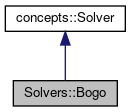
\includegraphics[width=170pt]{class_solvers_1_1_bogo__inherit__graph}
\end{center}
\end{figure}


Collaboration diagram for Solvers\+:\+:Bogo\+:\nopagebreak
\begin{figure}[H]
\begin{center}
\leavevmode
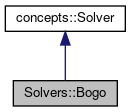
\includegraphics[width=170pt]{class_solvers_1_1_bogo__coll__graph}
\end{center}
\end{figure}
\subsection*{Public Member Functions}
\begin{DoxyCompactItemize}
\item 
\hyperlink{class_solvers_1_1_bogo_a2aa7f7e6b327254f789449a768dbf384}{Bogo} ()
\item 
\hyperlink{class_solvers_1_1_bogo}{Bogo} \& \hyperlink{class_solvers_1_1_bogo_a71508927ade20d8478509c1ec0ed7119}{set\+Nb\+Draws} (int log\+\_\+level)
\item 
\hyperlink{class_solvers_1_1_bogo}{Bogo} \& \hyperlink{class_solvers_1_1_bogo_ae47a955e952670eba66efad35c824023}{set\+Seed} (int seed)
\item 
\hyperlink{class_solution}{Solution} $\ast$ \hyperlink{class_solvers_1_1_bogo_a094c019a0efda929bd2369d2a47256f6}{solve} (const \hyperlink{class_landscape}{Landscape} \&landscape, const \hyperlink{class_restoration_plan}{Restoration\+Plan} \&plans, const double B) const
\item 
const std\+::string \hyperlink{class_solvers_1_1_bogo_a496539bab5a74757fe6d50e78e0a641f}{name} () const
\end{DoxyCompactItemize}
\subsection*{Additional Inherited Members}


\subsection{Constructor \& Destructor Documentation}
\mbox{\Hypertarget{class_solvers_1_1_bogo_a2aa7f7e6b327254f789449a768dbf384}\label{class_solvers_1_1_bogo_a2aa7f7e6b327254f789449a768dbf384}} 
\index{Solvers\+::\+Bogo@{Solvers\+::\+Bogo}!Bogo@{Bogo}}
\index{Bogo@{Bogo}!Solvers\+::\+Bogo@{Solvers\+::\+Bogo}}
\subsubsection{\texorpdfstring{Bogo()}{Bogo()}}
{\footnotesize\ttfamily Solvers\+::\+Bogo\+::\+Bogo (\begin{DoxyParamCaption}{ }\end{DoxyParamCaption})\hspace{0.3cm}{\ttfamily [inline]}}



\subsection{Member Function Documentation}
\mbox{\Hypertarget{class_solvers_1_1_bogo_a496539bab5a74757fe6d50e78e0a641f}\label{class_solvers_1_1_bogo_a496539bab5a74757fe6d50e78e0a641f}} 
\index{Solvers\+::\+Bogo@{Solvers\+::\+Bogo}!name@{name}}
\index{name@{name}!Solvers\+::\+Bogo@{Solvers\+::\+Bogo}}
\subsubsection{\texorpdfstring{name()}{name()}}
{\footnotesize\ttfamily const std\+::string Solvers\+::\+Bogo\+::name (\begin{DoxyParamCaption}{ }\end{DoxyParamCaption}) const\hspace{0.3cm}{\ttfamily [inline]}, {\ttfamily [virtual]}}



Implements \hyperlink{classconcepts_1_1_solver_ab995568318a506446228f45cab2fcce7}{concepts\+::\+Solver}.

\mbox{\Hypertarget{class_solvers_1_1_bogo_a71508927ade20d8478509c1ec0ed7119}\label{class_solvers_1_1_bogo_a71508927ade20d8478509c1ec0ed7119}} 
\index{Solvers\+::\+Bogo@{Solvers\+::\+Bogo}!set\+Nb\+Draws@{set\+Nb\+Draws}}
\index{set\+Nb\+Draws@{set\+Nb\+Draws}!Solvers\+::\+Bogo@{Solvers\+::\+Bogo}}
\subsubsection{\texorpdfstring{set\+Nb\+Draws()}{setNbDraws()}}
{\footnotesize\ttfamily \hyperlink{class_solvers_1_1_bogo}{Bogo}\& Solvers\+::\+Bogo\+::set\+Nb\+Draws (\begin{DoxyParamCaption}\item[{int}]{log\+\_\+level }\end{DoxyParamCaption})\hspace{0.3cm}{\ttfamily [inline]}}

\mbox{\Hypertarget{class_solvers_1_1_bogo_ae47a955e952670eba66efad35c824023}\label{class_solvers_1_1_bogo_ae47a955e952670eba66efad35c824023}} 
\index{Solvers\+::\+Bogo@{Solvers\+::\+Bogo}!set\+Seed@{set\+Seed}}
\index{set\+Seed@{set\+Seed}!Solvers\+::\+Bogo@{Solvers\+::\+Bogo}}
\subsubsection{\texorpdfstring{set\+Seed()}{setSeed()}}
{\footnotesize\ttfamily \hyperlink{class_solvers_1_1_bogo}{Bogo}\& Solvers\+::\+Bogo\+::set\+Seed (\begin{DoxyParamCaption}\item[{int}]{seed }\end{DoxyParamCaption})\hspace{0.3cm}{\ttfamily [inline]}}

\mbox{\Hypertarget{class_solvers_1_1_bogo_a094c019a0efda929bd2369d2a47256f6}\label{class_solvers_1_1_bogo_a094c019a0efda929bd2369d2a47256f6}} 
\index{Solvers\+::\+Bogo@{Solvers\+::\+Bogo}!solve@{solve}}
\index{solve@{solve}!Solvers\+::\+Bogo@{Solvers\+::\+Bogo}}
\subsubsection{\texorpdfstring{solve()}{solve()}}
{\footnotesize\ttfamily \hyperlink{class_solution}{Solution} $\ast$ Solvers\+::\+Bogo\+::solve (\begin{DoxyParamCaption}\item[{const \hyperlink{class_landscape}{Landscape} \&}]{landscape,  }\item[{const \hyperlink{class_restoration_plan}{Restoration\+Plan} \&}]{plans,  }\item[{const double}]{B }\end{DoxyParamCaption}) const\hspace{0.3cm}{\ttfamily [virtual]}}



Implements \hyperlink{classconcepts_1_1_solver_af323ad29df1e7b87facd7dc007568c80}{concepts\+::\+Solver}.



The documentation for this class was generated from the following files\+:\begin{DoxyCompactItemize}
\item 
/home/plaiseek/\+Projects/landscape\+\_\+opt\+\_\+cpp/include/solvers/\hyperlink{bogo_8hpp}{bogo.\+hpp}\item 
/home/plaiseek/\+Projects/landscape\+\_\+opt\+\_\+cpp/src/solvers/\hyperlink{bogo_8cpp}{bogo.\+cpp}\end{DoxyCompactItemize}

\hypertarget{class_chrono}{}\section{Chrono Class Reference}
\label{class_chrono}\index{Chrono@{Chrono}}


A simple chronometer class.  




{\ttfamily \#include $<$chrono.\+hpp$>$}

\subsection*{Public Member Functions}
\begin{DoxyCompactItemize}
\item 
\hyperlink{class_chrono_a3ac5e047174f389e7bd8aae71c6b5e8c}{Chrono} ()
\item 
void \hyperlink{class_chrono_a027be23720616639bc610a98c53740ea}{reset} ()
\item 
{\footnotesize template$<$class chrono\+\_\+unit $>$ }\\int \hyperlink{class_chrono_a224beb8f4bebc02d2a12dcf29ba6e5c9}{time} ()
\item 
int \hyperlink{class_chrono_ac358f9278ad6089d8fe626b3fe558590}{time\+Us} ()
\item 
int \hyperlink{class_chrono_a823638d3248d0cdd9f01ef6c840ad1d2}{time\+Ms} ()
\item 
int \hyperlink{class_chrono_a52c5348d69e89324a3430584cb760651}{timeS} ()
\item 
{\footnotesize template$<$class chrono\+\_\+unit $>$ }\\int \hyperlink{class_chrono_a3edbf874477c7342f066b539e7bc493c}{lap\+Time} ()
\item 
int \hyperlink{class_chrono_ab5ef782998bb0c75ecf7cf43db8ce8a0}{lap\+Time\+Us} ()
\item 
int \hyperlink{class_chrono_ab43a3526cac90d1c50da457c817cdef0}{lap\+Time\+Ms} ()
\item 
int \hyperlink{class_chrono_a91702be8978d2a969d27c2098ba41196}{lap\+TimeS} ()
\end{DoxyCompactItemize}


\subsection{Detailed Description}
A simple chronometer class. 

\subsection{Constructor \& Destructor Documentation}
\mbox{\Hypertarget{class_chrono_a3ac5e047174f389e7bd8aae71c6b5e8c}\label{class_chrono_a3ac5e047174f389e7bd8aae71c6b5e8c}} 
\index{Chrono@{Chrono}!Chrono@{Chrono}}
\index{Chrono@{Chrono}!Chrono@{Chrono}}
\subsubsection{\texorpdfstring{Chrono()}{Chrono()}}
{\footnotesize\ttfamily Chrono\+::\+Chrono (\begin{DoxyParamCaption}{ }\end{DoxyParamCaption})\hspace{0.3cm}{\ttfamily [inline]}}



\subsection{Member Function Documentation}
\mbox{\Hypertarget{class_chrono_a3edbf874477c7342f066b539e7bc493c}\label{class_chrono_a3edbf874477c7342f066b539e7bc493c}} 
\index{Chrono@{Chrono}!lap\+Time@{lap\+Time}}
\index{lap\+Time@{lap\+Time}!Chrono@{Chrono}}
\subsubsection{\texorpdfstring{lap\+Time()}{lapTime()}}
{\footnotesize\ttfamily template$<$class chrono\+\_\+unit $>$ \\
int Chrono\+::lap\+Time (\begin{DoxyParamCaption}{ }\end{DoxyParamCaption})\hspace{0.3cm}{\ttfamily [inline]}}

\mbox{\Hypertarget{class_chrono_ab43a3526cac90d1c50da457c817cdef0}\label{class_chrono_ab43a3526cac90d1c50da457c817cdef0}} 
\index{Chrono@{Chrono}!lap\+Time\+Ms@{lap\+Time\+Ms}}
\index{lap\+Time\+Ms@{lap\+Time\+Ms}!Chrono@{Chrono}}
\subsubsection{\texorpdfstring{lap\+Time\+Ms()}{lapTimeMs()}}
{\footnotesize\ttfamily int Chrono\+::lap\+Time\+Ms (\begin{DoxyParamCaption}{ }\end{DoxyParamCaption})\hspace{0.3cm}{\ttfamily [inline]}}

\mbox{\Hypertarget{class_chrono_a91702be8978d2a969d27c2098ba41196}\label{class_chrono_a91702be8978d2a969d27c2098ba41196}} 
\index{Chrono@{Chrono}!lap\+TimeS@{lap\+TimeS}}
\index{lap\+TimeS@{lap\+TimeS}!Chrono@{Chrono}}
\subsubsection{\texorpdfstring{lap\+Time\+S()}{lapTimeS()}}
{\footnotesize\ttfamily int Chrono\+::lap\+TimeS (\begin{DoxyParamCaption}{ }\end{DoxyParamCaption})\hspace{0.3cm}{\ttfamily [inline]}}

\mbox{\Hypertarget{class_chrono_ab5ef782998bb0c75ecf7cf43db8ce8a0}\label{class_chrono_ab5ef782998bb0c75ecf7cf43db8ce8a0}} 
\index{Chrono@{Chrono}!lap\+Time\+Us@{lap\+Time\+Us}}
\index{lap\+Time\+Us@{lap\+Time\+Us}!Chrono@{Chrono}}
\subsubsection{\texorpdfstring{lap\+Time\+Us()}{lapTimeUs()}}
{\footnotesize\ttfamily int Chrono\+::lap\+Time\+Us (\begin{DoxyParamCaption}{ }\end{DoxyParamCaption})\hspace{0.3cm}{\ttfamily [inline]}}

\mbox{\Hypertarget{class_chrono_a027be23720616639bc610a98c53740ea}\label{class_chrono_a027be23720616639bc610a98c53740ea}} 
\index{Chrono@{Chrono}!reset@{reset}}
\index{reset@{reset}!Chrono@{Chrono}}
\subsubsection{\texorpdfstring{reset()}{reset()}}
{\footnotesize\ttfamily void Chrono\+::reset (\begin{DoxyParamCaption}{ }\end{DoxyParamCaption})\hspace{0.3cm}{\ttfamily [inline]}}

\mbox{\Hypertarget{class_chrono_a224beb8f4bebc02d2a12dcf29ba6e5c9}\label{class_chrono_a224beb8f4bebc02d2a12dcf29ba6e5c9}} 
\index{Chrono@{Chrono}!time@{time}}
\index{time@{time}!Chrono@{Chrono}}
\subsubsection{\texorpdfstring{time()}{time()}}
{\footnotesize\ttfamily template$<$class chrono\+\_\+unit $>$ \\
int Chrono\+::time (\begin{DoxyParamCaption}{ }\end{DoxyParamCaption})\hspace{0.3cm}{\ttfamily [inline]}}

\mbox{\Hypertarget{class_chrono_a823638d3248d0cdd9f01ef6c840ad1d2}\label{class_chrono_a823638d3248d0cdd9f01ef6c840ad1d2}} 
\index{Chrono@{Chrono}!time\+Ms@{time\+Ms}}
\index{time\+Ms@{time\+Ms}!Chrono@{Chrono}}
\subsubsection{\texorpdfstring{time\+Ms()}{timeMs()}}
{\footnotesize\ttfamily int Chrono\+::time\+Ms (\begin{DoxyParamCaption}{ }\end{DoxyParamCaption})\hspace{0.3cm}{\ttfamily [inline]}}

\mbox{\Hypertarget{class_chrono_a52c5348d69e89324a3430584cb760651}\label{class_chrono_a52c5348d69e89324a3430584cb760651}} 
\index{Chrono@{Chrono}!timeS@{timeS}}
\index{timeS@{timeS}!Chrono@{Chrono}}
\subsubsection{\texorpdfstring{time\+S()}{timeS()}}
{\footnotesize\ttfamily int Chrono\+::timeS (\begin{DoxyParamCaption}{ }\end{DoxyParamCaption})\hspace{0.3cm}{\ttfamily [inline]}}

\mbox{\Hypertarget{class_chrono_ac358f9278ad6089d8fe626b3fe558590}\label{class_chrono_ac358f9278ad6089d8fe626b3fe558590}} 
\index{Chrono@{Chrono}!time\+Us@{time\+Us}}
\index{time\+Us@{time\+Us}!Chrono@{Chrono}}
\subsubsection{\texorpdfstring{time\+Us()}{timeUs()}}
{\footnotesize\ttfamily int Chrono\+::time\+Us (\begin{DoxyParamCaption}{ }\end{DoxyParamCaption})\hspace{0.3cm}{\ttfamily [inline]}}



The documentation for this class was generated from the following file\+:\begin{DoxyCompactItemize}
\item 
/home/plaiseek/\+Projects/landscape\+\_\+opt\+\_\+cpp/include/utils/\hyperlink{chrono_8hpp}{chrono.\+hpp}\end{DoxyCompactItemize}

\hypertarget{classconcepts_1_1_connectivity_index}{}\section{concepts\+:\+:Connectivity\+Index Class Reference}
\label{classconcepts_1_1_connectivity_index}\index{concepts\+::\+Connectivity\+Index@{concepts\+::\+Connectivity\+Index}}


{\ttfamily \#include $<$connectivity\+\_\+index.\+hpp$>$}



Inheritance diagram for concepts\+:\+:Connectivity\+Index\+:\nopagebreak
\begin{figure}[H]
\begin{center}
\leavevmode
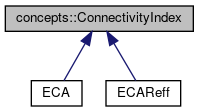
\includegraphics[width=221pt]{classconcepts_1_1_connectivity_index__inherit__graph}
\end{center}
\end{figure}


Collaboration diagram for concepts\+:\+:Connectivity\+Index\+:\nopagebreak
\begin{figure}[H]
\begin{center}
\leavevmode
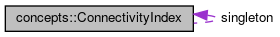
\includegraphics[width=282pt]{classconcepts_1_1_connectivity_index__coll__graph}
\end{center}
\end{figure}
\subsection*{Public Member Functions}
\begin{DoxyCompactItemize}
\item 
\hyperlink{classconcepts_1_1_connectivity_index_aa0ca6c18e8caeb3bc8882e7ce4fc0588}{$\sim$\+Connectivity\+Index} ()
\item 
{\footnotesize template$<$typename GR , typename QM , typename DM $>$ }\\double \hyperlink{classconcepts_1_1_connectivity_index_a1718c62ef509fabe0ad1a54cf5a9b0ce}{eval} (const \hyperlink{classconcepts_1_1_abstract_landscape}{concepts\+::\+Abstract\+Landscape}$<$ GR, QM, DM $>$ \&landscape)
\end{DoxyCompactItemize}
\subsection*{Static Public Member Functions}
\begin{DoxyCompactItemize}
\item 
static \hyperlink{classconcepts_1_1_connectivity_index}{Connectivity\+Index} \& \hyperlink{classconcepts_1_1_connectivity_index_a4305f910870c1b5de783d770b35fea09}{get} () noexcept
\end{DoxyCompactItemize}
\subsection*{Protected Member Functions}
\begin{DoxyCompactItemize}
\item 
\hyperlink{classconcepts_1_1_connectivity_index_a6c6bf75148055bdafb48c3d990b10968}{Connectivity\+Index} ()
\end{DoxyCompactItemize}
\subsection*{Static Protected Attributes}
\begin{DoxyCompactItemize}
\item 
static \hyperlink{classconcepts_1_1_connectivity_index}{Connectivity\+Index} \hyperlink{classconcepts_1_1_connectivity_index_a6c3d718aa3d0a00d648560ea0ef89eb4}{singleton}
\end{DoxyCompactItemize}


\subsection{Constructor \& Destructor Documentation}
\mbox{\Hypertarget{classconcepts_1_1_connectivity_index_a6c6bf75148055bdafb48c3d990b10968}\label{classconcepts_1_1_connectivity_index_a6c6bf75148055bdafb48c3d990b10968}} 
\index{concepts\+::\+Connectivity\+Index@{concepts\+::\+Connectivity\+Index}!Connectivity\+Index@{Connectivity\+Index}}
\index{Connectivity\+Index@{Connectivity\+Index}!concepts\+::\+Connectivity\+Index@{concepts\+::\+Connectivity\+Index}}
\subsubsection{\texorpdfstring{Connectivity\+Index()}{ConnectivityIndex()}}
{\footnotesize\ttfamily concepts\+::\+Connectivity\+Index\+::\+Connectivity\+Index (\begin{DoxyParamCaption}{ }\end{DoxyParamCaption})\hspace{0.3cm}{\ttfamily [inline]}, {\ttfamily [protected]}}

\mbox{\Hypertarget{classconcepts_1_1_connectivity_index_aa0ca6c18e8caeb3bc8882e7ce4fc0588}\label{classconcepts_1_1_connectivity_index_aa0ca6c18e8caeb3bc8882e7ce4fc0588}} 
\index{concepts\+::\+Connectivity\+Index@{concepts\+::\+Connectivity\+Index}!````~Connectivity\+Index@{$\sim$\+Connectivity\+Index}}
\index{````~Connectivity\+Index@{$\sim$\+Connectivity\+Index}!concepts\+::\+Connectivity\+Index@{concepts\+::\+Connectivity\+Index}}
\subsubsection{\texorpdfstring{$\sim$\+Connectivity\+Index()}{~ConnectivityIndex()}}
{\footnotesize\ttfamily concepts\+::\+Connectivity\+Index\+::$\sim$\+Connectivity\+Index (\begin{DoxyParamCaption}{ }\end{DoxyParamCaption})\hspace{0.3cm}{\ttfamily [inline]}}



\subsection{Member Function Documentation}
\mbox{\Hypertarget{classconcepts_1_1_connectivity_index_a1718c62ef509fabe0ad1a54cf5a9b0ce}\label{classconcepts_1_1_connectivity_index_a1718c62ef509fabe0ad1a54cf5a9b0ce}} 
\index{concepts\+::\+Connectivity\+Index@{concepts\+::\+Connectivity\+Index}!eval@{eval}}
\index{eval@{eval}!concepts\+::\+Connectivity\+Index@{concepts\+::\+Connectivity\+Index}}
\subsubsection{\texorpdfstring{eval()}{eval()}}
{\footnotesize\ttfamily template$<$typename GR , typename QM , typename DM $>$ \\
double concepts\+::\+Connectivity\+Index\+::eval (\begin{DoxyParamCaption}\item[{const \hyperlink{classconcepts_1_1_abstract_landscape}{concepts\+::\+Abstract\+Landscape}$<$ GR, QM, DM $>$ \&}]{landscape }\end{DoxyParamCaption})\hspace{0.3cm}{\ttfamily [inline]}}

\mbox{\Hypertarget{classconcepts_1_1_connectivity_index_a4305f910870c1b5de783d770b35fea09}\label{classconcepts_1_1_connectivity_index_a4305f910870c1b5de783d770b35fea09}} 
\index{concepts\+::\+Connectivity\+Index@{concepts\+::\+Connectivity\+Index}!get@{get}}
\index{get@{get}!concepts\+::\+Connectivity\+Index@{concepts\+::\+Connectivity\+Index}}
\subsubsection{\texorpdfstring{get()}{get()}}
{\footnotesize\ttfamily static \hyperlink{classconcepts_1_1_connectivity_index}{Connectivity\+Index}\& concepts\+::\+Connectivity\+Index\+::get (\begin{DoxyParamCaption}{ }\end{DoxyParamCaption})\hspace{0.3cm}{\ttfamily [inline]}, {\ttfamily [static]}, {\ttfamily [noexcept]}}



\subsection{Member Data Documentation}
\mbox{\Hypertarget{classconcepts_1_1_connectivity_index_a6c3d718aa3d0a00d648560ea0ef89eb4}\label{classconcepts_1_1_connectivity_index_a6c3d718aa3d0a00d648560ea0ef89eb4}} 
\index{concepts\+::\+Connectivity\+Index@{concepts\+::\+Connectivity\+Index}!singleton@{singleton}}
\index{singleton@{singleton}!concepts\+::\+Connectivity\+Index@{concepts\+::\+Connectivity\+Index}}
\subsubsection{\texorpdfstring{singleton}{singleton}}
{\footnotesize\ttfamily \hyperlink{classconcepts_1_1_connectivity_index}{Connectivity\+Index} concepts\+::\+Connectivity\+Index\+::singleton\hspace{0.3cm}{\ttfamily [static]}, {\ttfamily [protected]}}



The documentation for this class was generated from the following file\+:\begin{DoxyCompactItemize}
\item 
/home/plaiseek/\+Projects/landscape\+\_\+opt\+\_\+cpp/include/indices/concept/\hyperlink{connectivity__index_8hpp}{connectivity\+\_\+index.\+hpp}\end{DoxyCompactItemize}

\hypertarget{class_solvers_1_1_p_l___e_c_a__3___vars_1_1_contracted_vars}{}\section{Solvers\+:\+:P\+L\+\_\+\+E\+C\+A\+\_\+3\+\_\+\+Vars\+:\+:Contracted\+Vars Class Reference}
\label{class_solvers_1_1_p_l___e_c_a__3___vars_1_1_contracted_vars}\index{Solvers\+::\+P\+L\+\_\+\+E\+C\+A\+\_\+3\+\_\+\+Vars\+::\+Contracted\+Vars@{Solvers\+::\+P\+L\+\_\+\+E\+C\+A\+\_\+3\+\_\+\+Vars\+::\+Contracted\+Vars}}


Collaboration diagram for Solvers\+:\+:P\+L\+\_\+\+E\+C\+A\+\_\+3\+\_\+\+Vars\+:\+:Contracted\+Vars\+:\nopagebreak
\begin{figure}[H]
\begin{center}
\leavevmode
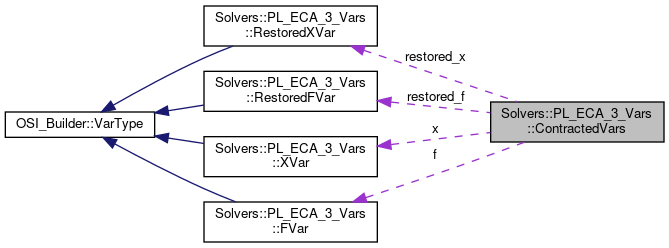
\includegraphics[width=350pt]{class_solvers_1_1_p_l___e_c_a__3___vars_1_1_contracted_vars__coll__graph}
\end{center}
\end{figure}
\subsection*{Public Member Functions}
\begin{DoxyCompactItemize}
\item 
\hyperlink{class_solvers_1_1_p_l___e_c_a__3___vars_1_1_contracted_vars_a009b20895de54f1395647d5d0f11f79e}{Contracted\+Vars} (const \hyperlink{class_contraction_result}{Contraction\+Result} \&cr)
\end{DoxyCompactItemize}
\subsection*{Public Attributes}
\begin{DoxyCompactItemize}
\item 
\hyperlink{class_solvers_1_1_p_l___e_c_a__3___vars_1_1_x_var}{X\+Var} \hyperlink{class_solvers_1_1_p_l___e_c_a__3___vars_1_1_contracted_vars_a514a3404b83c008b3273eccf66bb6fcb}{x}
\item 
\hyperlink{class_solvers_1_1_p_l___e_c_a__3___vars_1_1_restored_x_var}{Restored\+X\+Var} \hyperlink{class_solvers_1_1_p_l___e_c_a__3___vars_1_1_contracted_vars_a3ae6936df398cd301edd534f11129e11}{restored\+\_\+x}
\item 
\hyperlink{class_solvers_1_1_p_l___e_c_a__3___vars_1_1_f_var}{F\+Var} \hyperlink{class_solvers_1_1_p_l___e_c_a__3___vars_1_1_contracted_vars_a746123dd243f06f242afa1d946b96c21}{f}
\item 
\hyperlink{class_solvers_1_1_p_l___e_c_a__3___vars_1_1_restored_f_var}{Restored\+F\+Var} \hyperlink{class_solvers_1_1_p_l___e_c_a__3___vars_1_1_contracted_vars_a566857b0095b735578b548cce057f904}{restored\+\_\+f}
\end{DoxyCompactItemize}


\subsection{Constructor \& Destructor Documentation}
\mbox{\Hypertarget{class_solvers_1_1_p_l___e_c_a__3___vars_1_1_contracted_vars_a009b20895de54f1395647d5d0f11f79e}\label{class_solvers_1_1_p_l___e_c_a__3___vars_1_1_contracted_vars_a009b20895de54f1395647d5d0f11f79e}} 
\index{Solvers\+::\+P\+L\+\_\+\+E\+C\+A\+\_\+3\+\_\+\+Vars\+::\+Contracted\+Vars@{Solvers\+::\+P\+L\+\_\+\+E\+C\+A\+\_\+3\+\_\+\+Vars\+::\+Contracted\+Vars}!Contracted\+Vars@{Contracted\+Vars}}
\index{Contracted\+Vars@{Contracted\+Vars}!Solvers\+::\+P\+L\+\_\+\+E\+C\+A\+\_\+3\+\_\+\+Vars\+::\+Contracted\+Vars@{Solvers\+::\+P\+L\+\_\+\+E\+C\+A\+\_\+3\+\_\+\+Vars\+::\+Contracted\+Vars}}
\subsubsection{\texorpdfstring{Contracted\+Vars()}{ContractedVars()}}
{\footnotesize\ttfamily Solvers\+::\+P\+L\+\_\+\+E\+C\+A\+\_\+3\+\_\+\+Vars\+::\+Contracted\+Vars\+::\+Contracted\+Vars (\begin{DoxyParamCaption}\item[{const \hyperlink{class_contraction_result}{Contraction\+Result} \&}]{cr }\end{DoxyParamCaption})\hspace{0.3cm}{\ttfamily [inline]}}



\subsection{Member Data Documentation}
\mbox{\Hypertarget{class_solvers_1_1_p_l___e_c_a__3___vars_1_1_contracted_vars_a746123dd243f06f242afa1d946b96c21}\label{class_solvers_1_1_p_l___e_c_a__3___vars_1_1_contracted_vars_a746123dd243f06f242afa1d946b96c21}} 
\index{Solvers\+::\+P\+L\+\_\+\+E\+C\+A\+\_\+3\+\_\+\+Vars\+::\+Contracted\+Vars@{Solvers\+::\+P\+L\+\_\+\+E\+C\+A\+\_\+3\+\_\+\+Vars\+::\+Contracted\+Vars}!f@{f}}
\index{f@{f}!Solvers\+::\+P\+L\+\_\+\+E\+C\+A\+\_\+3\+\_\+\+Vars\+::\+Contracted\+Vars@{Solvers\+::\+P\+L\+\_\+\+E\+C\+A\+\_\+3\+\_\+\+Vars\+::\+Contracted\+Vars}}
\subsubsection{\texorpdfstring{f}{f}}
{\footnotesize\ttfamily \hyperlink{class_solvers_1_1_p_l___e_c_a__3___vars_1_1_f_var}{F\+Var} Solvers\+::\+P\+L\+\_\+\+E\+C\+A\+\_\+3\+\_\+\+Vars\+::\+Contracted\+Vars\+::f}

\mbox{\Hypertarget{class_solvers_1_1_p_l___e_c_a__3___vars_1_1_contracted_vars_a566857b0095b735578b548cce057f904}\label{class_solvers_1_1_p_l___e_c_a__3___vars_1_1_contracted_vars_a566857b0095b735578b548cce057f904}} 
\index{Solvers\+::\+P\+L\+\_\+\+E\+C\+A\+\_\+3\+\_\+\+Vars\+::\+Contracted\+Vars@{Solvers\+::\+P\+L\+\_\+\+E\+C\+A\+\_\+3\+\_\+\+Vars\+::\+Contracted\+Vars}!restored\+\_\+f@{restored\+\_\+f}}
\index{restored\+\_\+f@{restored\+\_\+f}!Solvers\+::\+P\+L\+\_\+\+E\+C\+A\+\_\+3\+\_\+\+Vars\+::\+Contracted\+Vars@{Solvers\+::\+P\+L\+\_\+\+E\+C\+A\+\_\+3\+\_\+\+Vars\+::\+Contracted\+Vars}}
\subsubsection{\texorpdfstring{restored\+\_\+f}{restored\_f}}
{\footnotesize\ttfamily \hyperlink{class_solvers_1_1_p_l___e_c_a__3___vars_1_1_restored_f_var}{Restored\+F\+Var} Solvers\+::\+P\+L\+\_\+\+E\+C\+A\+\_\+3\+\_\+\+Vars\+::\+Contracted\+Vars\+::restored\+\_\+f}

\mbox{\Hypertarget{class_solvers_1_1_p_l___e_c_a__3___vars_1_1_contracted_vars_a3ae6936df398cd301edd534f11129e11}\label{class_solvers_1_1_p_l___e_c_a__3___vars_1_1_contracted_vars_a3ae6936df398cd301edd534f11129e11}} 
\index{Solvers\+::\+P\+L\+\_\+\+E\+C\+A\+\_\+3\+\_\+\+Vars\+::\+Contracted\+Vars@{Solvers\+::\+P\+L\+\_\+\+E\+C\+A\+\_\+3\+\_\+\+Vars\+::\+Contracted\+Vars}!restored\+\_\+x@{restored\+\_\+x}}
\index{restored\+\_\+x@{restored\+\_\+x}!Solvers\+::\+P\+L\+\_\+\+E\+C\+A\+\_\+3\+\_\+\+Vars\+::\+Contracted\+Vars@{Solvers\+::\+P\+L\+\_\+\+E\+C\+A\+\_\+3\+\_\+\+Vars\+::\+Contracted\+Vars}}
\subsubsection{\texorpdfstring{restored\+\_\+x}{restored\_x}}
{\footnotesize\ttfamily \hyperlink{class_solvers_1_1_p_l___e_c_a__3___vars_1_1_restored_x_var}{Restored\+X\+Var} Solvers\+::\+P\+L\+\_\+\+E\+C\+A\+\_\+3\+\_\+\+Vars\+::\+Contracted\+Vars\+::restored\+\_\+x}

\mbox{\Hypertarget{class_solvers_1_1_p_l___e_c_a__3___vars_1_1_contracted_vars_a514a3404b83c008b3273eccf66bb6fcb}\label{class_solvers_1_1_p_l___e_c_a__3___vars_1_1_contracted_vars_a514a3404b83c008b3273eccf66bb6fcb}} 
\index{Solvers\+::\+P\+L\+\_\+\+E\+C\+A\+\_\+3\+\_\+\+Vars\+::\+Contracted\+Vars@{Solvers\+::\+P\+L\+\_\+\+E\+C\+A\+\_\+3\+\_\+\+Vars\+::\+Contracted\+Vars}!x@{x}}
\index{x@{x}!Solvers\+::\+P\+L\+\_\+\+E\+C\+A\+\_\+3\+\_\+\+Vars\+::\+Contracted\+Vars@{Solvers\+::\+P\+L\+\_\+\+E\+C\+A\+\_\+3\+\_\+\+Vars\+::\+Contracted\+Vars}}
\subsubsection{\texorpdfstring{x}{x}}
{\footnotesize\ttfamily \hyperlink{class_solvers_1_1_p_l___e_c_a__3___vars_1_1_x_var}{X\+Var} Solvers\+::\+P\+L\+\_\+\+E\+C\+A\+\_\+3\+\_\+\+Vars\+::\+Contracted\+Vars\+::x}



The documentation for this class was generated from the following file\+:\begin{DoxyCompactItemize}
\item 
/home/plaiseek/\+Projects/landscape\+\_\+opt\+\_\+cpp/src/solvers/\hyperlink{pl__eca__3_8cpp}{pl\+\_\+eca\+\_\+3.\+cpp}\end{DoxyCompactItemize}

\hypertarget{class_contraction_precomputation}{}\section{Contraction\+Precomputation Class Reference}
\label{class_contraction_precomputation}\index{Contraction\+Precomputation@{Contraction\+Precomputation}}


{\ttfamily \#include $<$contraction\+\_\+precomputation.\+hpp$>$}



Inheritance diagram for Contraction\+Precomputation\+:\nopagebreak
\begin{figure}[H]
\begin{center}
\leavevmode
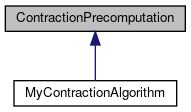
\includegraphics[width=215pt]{class_contraction_precomputation__inherit__graph}
\end{center}
\end{figure}
\subsection*{Public Member Functions}
\begin{DoxyCompactItemize}
\item 
void \hyperlink{class_contraction_precomputation_ab4ae0b053d4cb51b2d2c4d07027ee2b7}{erase\+\_\+non\+\_\+connected} (\hyperlink{class_landscape}{Landscape} \&landscape, Graph\+\_\+t\+::\+Node t) const
\item 
void \hyperlink{class_contraction_precomputation_a6cbc9c5ee6d4ec9a5092d6e624922396}{contract\+\_\+arc} (\hyperlink{class_landscape}{Landscape} \&contracted\+\_\+landscape, \hyperlink{class_restoration_plan}{Restoration\+Plan} \&plan, Graph\+\_\+t\+::\+Arc a) const
\item 
void \hyperlink{class_contraction_precomputation_a6ea4ee46a1805ced601de847969cab61}{model\+\_\+quality\+\_\+gains} (\hyperlink{class_landscape}{Landscape} \&landscape, \hyperlink{class_restoration_plan}{Restoration\+Plan} \&plan, std\+::vector$<$ std\+::vector$<$ Graph\+\_\+t\+::\+Arc $>$$>$ \&options\+\_\+nodes) const
\item 
void \hyperlink{class_contraction_precomputation_a6749c81605043e4398c80b49293b44c6}{retrive\+\_\+quality\+\_\+gains} (\hyperlink{class_landscape}{Landscape} \&landscape, \hyperlink{class_restoration_plan}{Restoration\+Plan} \&plan, const std\+::vector$<$ std\+::vector$<$ Graph\+\_\+t\+::\+Arc $>$$>$ \&options\+\_\+nodes) const
\item 
virtual Graph\+\_\+t\+::\+Node\+Map$<$ \hyperlink{class_contraction_result}{Contraction\+Result} $>$ $\ast$ \hyperlink{class_contraction_precomputation_a205ee98224bfa783a7ab27d3a986468b}{precompute} (const \hyperlink{class_landscape}{Landscape} \&landscape, const \hyperlink{class_restoration_plan}{Restoration\+Plan} \&plan) const =0
\end{DoxyCompactItemize}


\subsection{Member Function Documentation}
\mbox{\Hypertarget{class_contraction_precomputation_a6cbc9c5ee6d4ec9a5092d6e624922396}\label{class_contraction_precomputation_a6cbc9c5ee6d4ec9a5092d6e624922396}} 
\index{Contraction\+Precomputation@{Contraction\+Precomputation}!contract\+\_\+arc@{contract\+\_\+arc}}
\index{contract\+\_\+arc@{contract\+\_\+arc}!Contraction\+Precomputation@{Contraction\+Precomputation}}
\subsubsection{\texorpdfstring{contract\+\_\+arc()}{contract\_arc()}}
{\footnotesize\ttfamily void Contraction\+Precomputation\+::contract\+\_\+arc (\begin{DoxyParamCaption}\item[{\hyperlink{class_landscape}{Landscape} \&}]{landscape,  }\item[{\hyperlink{class_restoration_plan}{Restoration\+Plan} \&}]{plan,  }\item[{Graph\+\_\+t\+::\+Arc}]{a }\end{DoxyParamCaption}) const}

Contracts specified uv arc preserving graph ids

\begin{DoxyRefDesc}{Time Complexity}
\item[\hyperlink{time__time000002}{Time Complexity}]$O(deg(u))$ \end{DoxyRefDesc}
\begin{DoxyRefDesc}{Space Complexity}
\item[\hyperlink{space__space000002}{Space Complexity}]$O(deg(u))$ \end{DoxyRefDesc}
\mbox{\Hypertarget{class_contraction_precomputation_ab4ae0b053d4cb51b2d2c4d07027ee2b7}\label{class_contraction_precomputation_ab4ae0b053d4cb51b2d2c4d07027ee2b7}} 
\index{Contraction\+Precomputation@{Contraction\+Precomputation}!erase\+\_\+non\+\_\+connected@{erase\+\_\+non\+\_\+connected}}
\index{erase\+\_\+non\+\_\+connected@{erase\+\_\+non\+\_\+connected}!Contraction\+Precomputation@{Contraction\+Precomputation}}
\subsubsection{\texorpdfstring{erase\+\_\+non\+\_\+connected()}{erase\_non\_connected()}}
{\footnotesize\ttfamily void Contraction\+Precomputation\+::erase\+\_\+non\+\_\+connected (\begin{DoxyParamCaption}\item[{\hyperlink{class_landscape}{Landscape} \&}]{landscape,  }\item[{Graph\+\_\+t\+::\+Node}]{t }\end{DoxyParamCaption}) const}

Erase the nodes from wich there is not path to t

\begin{DoxyRefDesc}{Time Complexity}
\item[\hyperlink{time__time000001}{Time Complexity}]$O(V)$ \end{DoxyRefDesc}
\begin{DoxyRefDesc}{Space Complexity}
\item[\hyperlink{space__space000001}{Space Complexity}]$O(V)$ \end{DoxyRefDesc}
\mbox{\Hypertarget{class_contraction_precomputation_a6ea4ee46a1805ced601de847969cab61}\label{class_contraction_precomputation_a6ea4ee46a1805ced601de847969cab61}} 
\index{Contraction\+Precomputation@{Contraction\+Precomputation}!model\+\_\+quality\+\_\+gains@{model\+\_\+quality\+\_\+gains}}
\index{model\+\_\+quality\+\_\+gains@{model\+\_\+quality\+\_\+gains}!Contraction\+Precomputation@{Contraction\+Precomputation}}
\subsubsection{\texorpdfstring{model\+\_\+quality\+\_\+gains()}{model\_quality\_gains()}}
{\footnotesize\ttfamily void Contraction\+Precomputation\+::model\+\_\+quality\+\_\+gains (\begin{DoxyParamCaption}\item[{\hyperlink{class_landscape}{Landscape} \&}]{landscape,  }\item[{\hyperlink{class_restoration_plan}{Restoration\+Plan} \&}]{plan,  }\item[{std\+::vector$<$ std\+::vector$<$ Graph\+\_\+t\+::\+Arc $>$$>$ \&}]{options\+\_\+nodes }\end{DoxyParamCaption}) const}

Model quality gains options by appending nodes in the \hyperlink{class_landscape}{Landscape} and saves the arcs created in the vector passed by reference.

\begin{DoxyRefDesc}{Time Complexity}
\item[\hyperlink{time__time000003}{Time Complexity}]$O(\#options)$ \end{DoxyRefDesc}
\begin{DoxyRefDesc}{Space Complexity}
\item[\hyperlink{space__space000003}{Space Complexity}]$O(\#options)$ \end{DoxyRefDesc}
\mbox{\Hypertarget{class_contraction_precomputation_a205ee98224bfa783a7ab27d3a986468b}\label{class_contraction_precomputation_a205ee98224bfa783a7ab27d3a986468b}} 
\index{Contraction\+Precomputation@{Contraction\+Precomputation}!precompute@{precompute}}
\index{precompute@{precompute}!Contraction\+Precomputation@{Contraction\+Precomputation}}
\subsubsection{\texorpdfstring{precompute()}{precompute()}}
{\footnotesize\ttfamily virtual Graph\+\_\+t\+::\+Node\+Map$<$\hyperlink{class_contraction_result}{Contraction\+Result}$>$$\ast$ Contraction\+Precomputation\+::precompute (\begin{DoxyParamCaption}\item[{const \hyperlink{class_landscape}{Landscape} \&}]{landscape,  }\item[{const \hyperlink{class_restoration_plan}{Restoration\+Plan} \&}]{plan }\end{DoxyParamCaption}) const\hspace{0.3cm}{\ttfamily [pure virtual]}}



Implemented in \hyperlink{class_my_contraction_algorithm_a4583c564e68d337bd9dcef315093bbe6}{My\+Contraction\+Algorithm}.

\mbox{\Hypertarget{class_contraction_precomputation_a6749c81605043e4398c80b49293b44c6}\label{class_contraction_precomputation_a6749c81605043e4398c80b49293b44c6}} 
\index{Contraction\+Precomputation@{Contraction\+Precomputation}!retrive\+\_\+quality\+\_\+gains@{retrive\+\_\+quality\+\_\+gains}}
\index{retrive\+\_\+quality\+\_\+gains@{retrive\+\_\+quality\+\_\+gains}!Contraction\+Precomputation@{Contraction\+Precomputation}}
\subsubsection{\texorpdfstring{retrive\+\_\+quality\+\_\+gains()}{retrive\_quality\_gains()}}
{\footnotesize\ttfamily void Contraction\+Precomputation\+::retrive\+\_\+quality\+\_\+gains (\begin{DoxyParamCaption}\item[{\hyperlink{class_landscape}{Landscape} \&}]{landscape,  }\item[{\hyperlink{class_restoration_plan}{Restoration\+Plan} \&}]{plan,  }\item[{const std\+::vector$<$ std\+::vector$<$ Graph\+\_\+t\+::\+Arc $>$$>$ \&}]{options\+\_\+nodes }\end{DoxyParamCaption}) const}

Retrives quality gains options by deleting previously added nodes in the \hyperlink{class_landscape}{Landscape} and reconstruct the corresponding option.

\begin{DoxyRefDesc}{Time Complexity}
\item[\hyperlink{time__time000004}{Time Complexity}]$O(\#options)$ \end{DoxyRefDesc}
\begin{DoxyRefDesc}{Space Complexity}
\item[\hyperlink{space__space000004}{Space Complexity}]$O(\#options)$ \end{DoxyRefDesc}


The documentation for this class was generated from the following files\+:\begin{DoxyCompactItemize}
\item 
/home/plaiseek/\+Projects/landscape\+\_\+opt\+\_\+cpp/include/precomputation/concept/\hyperlink{contraction__precomputation_8hpp}{contraction\+\_\+precomputation.\+hpp}\item 
/home/plaiseek/\+Projects/landscape\+\_\+opt\+\_\+cpp/src/precomputation/concept/\hyperlink{contraction__precomputation_8cpp}{contraction\+\_\+precomputation.\+cpp}\end{DoxyCompactItemize}

\hypertarget{class_contraction_result}{}\section{Contraction\+Result Class Reference}
\label{class_contraction_result}\index{Contraction\+Result@{Contraction\+Result}}


{\ttfamily \#include $<$contraction\+\_\+precomputation.\+hpp$>$}

\subsection*{Public Member Functions}
\begin{DoxyCompactItemize}
\item 
\hyperlink{class_contraction_result_ac4942aaf3506bbd80a7b8bf1f9d070fe}{Contraction\+Result} ()
\item 
\hyperlink{class_contraction_result_aa63254d104eb42e70978a6a864ce350e}{Contraction\+Result} (\hyperlink{class_landscape}{Landscape} $\ast$l, \hyperlink{class_restoration_plan}{Restoration\+Plan} $\ast$p, Graph\+\_\+t\+::\+Node \hyperlink{class_contraction_result_a73086d90a83967d2cf24c7dd9fc83cd9}{t})
\item 
\hyperlink{class_contraction_result_a2fc9653548df2d9499388f1af8280615}{$\sim$\+Contraction\+Result} ()
\end{DoxyCompactItemize}
\subsection*{Public Attributes}
\begin{DoxyCompactItemize}
\item 
std\+::shared\+\_\+ptr$<$ \hyperlink{class_landscape}{Landscape} $>$ \hyperlink{class_contraction_result_ab2693f752e287b3f6d031e80f0368240}{landscape}
\item 
std\+::shared\+\_\+ptr$<$ \hyperlink{class_restoration_plan}{Restoration\+Plan} $>$ \hyperlink{class_contraction_result_aa684d24bad0d74858c604bb4dc070aa3}{plan}
\item 
Graph\+\_\+t\+::\+Node \hyperlink{class_contraction_result_a73086d90a83967d2cf24c7dd9fc83cd9}{t}
\end{DoxyCompactItemize}


\subsection{Constructor \& Destructor Documentation}
\mbox{\Hypertarget{class_contraction_result_ac4942aaf3506bbd80a7b8bf1f9d070fe}\label{class_contraction_result_ac4942aaf3506bbd80a7b8bf1f9d070fe}} 
\index{Contraction\+Result@{Contraction\+Result}!Contraction\+Result@{Contraction\+Result}}
\index{Contraction\+Result@{Contraction\+Result}!Contraction\+Result@{Contraction\+Result}}
\subsubsection{\texorpdfstring{Contraction\+Result()}{ContractionResult()}\hspace{0.1cm}{\footnotesize\ttfamily [1/2]}}
{\footnotesize\ttfamily Contraction\+Result\+::\+Contraction\+Result (\begin{DoxyParamCaption}{ }\end{DoxyParamCaption})\hspace{0.3cm}{\ttfamily [inline]}}

\mbox{\Hypertarget{class_contraction_result_aa63254d104eb42e70978a6a864ce350e}\label{class_contraction_result_aa63254d104eb42e70978a6a864ce350e}} 
\index{Contraction\+Result@{Contraction\+Result}!Contraction\+Result@{Contraction\+Result}}
\index{Contraction\+Result@{Contraction\+Result}!Contraction\+Result@{Contraction\+Result}}
\subsubsection{\texorpdfstring{Contraction\+Result()}{ContractionResult()}\hspace{0.1cm}{\footnotesize\ttfamily [2/2]}}
{\footnotesize\ttfamily Contraction\+Result\+::\+Contraction\+Result (\begin{DoxyParamCaption}\item[{\hyperlink{class_landscape}{Landscape} $\ast$}]{l,  }\item[{\hyperlink{class_restoration_plan}{Restoration\+Plan} $\ast$}]{p,  }\item[{Graph\+\_\+t\+::\+Node}]{t }\end{DoxyParamCaption})\hspace{0.3cm}{\ttfamily [inline]}}

\mbox{\Hypertarget{class_contraction_result_a2fc9653548df2d9499388f1af8280615}\label{class_contraction_result_a2fc9653548df2d9499388f1af8280615}} 
\index{Contraction\+Result@{Contraction\+Result}!````~Contraction\+Result@{$\sim$\+Contraction\+Result}}
\index{````~Contraction\+Result@{$\sim$\+Contraction\+Result}!Contraction\+Result@{Contraction\+Result}}
\subsubsection{\texorpdfstring{$\sim$\+Contraction\+Result()}{~ContractionResult()}}
{\footnotesize\ttfamily Contraction\+Result\+::$\sim$\+Contraction\+Result (\begin{DoxyParamCaption}{ }\end{DoxyParamCaption})\hspace{0.3cm}{\ttfamily [inline]}}



\subsection{Member Data Documentation}
\mbox{\Hypertarget{class_contraction_result_ab2693f752e287b3f6d031e80f0368240}\label{class_contraction_result_ab2693f752e287b3f6d031e80f0368240}} 
\index{Contraction\+Result@{Contraction\+Result}!landscape@{landscape}}
\index{landscape@{landscape}!Contraction\+Result@{Contraction\+Result}}
\subsubsection{\texorpdfstring{landscape}{landscape}}
{\footnotesize\ttfamily std\+::shared\+\_\+ptr$<$\hyperlink{class_landscape}{Landscape}$>$ Contraction\+Result\+::landscape}

\mbox{\Hypertarget{class_contraction_result_aa684d24bad0d74858c604bb4dc070aa3}\label{class_contraction_result_aa684d24bad0d74858c604bb4dc070aa3}} 
\index{Contraction\+Result@{Contraction\+Result}!plan@{plan}}
\index{plan@{plan}!Contraction\+Result@{Contraction\+Result}}
\subsubsection{\texorpdfstring{plan}{plan}}
{\footnotesize\ttfamily std\+::shared\+\_\+ptr$<$\hyperlink{class_restoration_plan}{Restoration\+Plan}$>$ Contraction\+Result\+::plan}

\mbox{\Hypertarget{class_contraction_result_a73086d90a83967d2cf24c7dd9fc83cd9}\label{class_contraction_result_a73086d90a83967d2cf24c7dd9fc83cd9}} 
\index{Contraction\+Result@{Contraction\+Result}!t@{t}}
\index{t@{t}!Contraction\+Result@{Contraction\+Result}}
\subsubsection{\texorpdfstring{t}{t}}
{\footnotesize\ttfamily Graph\+\_\+t\+::\+Node Contraction\+Result\+::t}



The documentation for this class was generated from the following file\+:\begin{DoxyCompactItemize}
\item 
/home/plaiseek/\+Projects/landscape\+\_\+opt\+\_\+cpp/include/precomputation/concept/\hyperlink{contraction__precomputation_8hpp}{contraction\+\_\+precomputation.\+hpp}\end{DoxyCompactItemize}

\hypertarget{class_decored_landscape}{}\section{Decored\+Landscape Class Reference}
\label{class_decored_landscape}\index{Decored\+Landscape@{Decored\+Landscape}}


Class that represent an decored landscape.  




{\ttfamily \#include $<$decored\+\_\+landscape.\+hpp$>$}



Inheritance diagram for Decored\+Landscape\+:\nopagebreak
\begin{figure}[H]
\begin{center}
\leavevmode
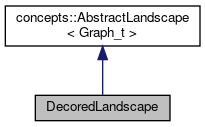
\includegraphics[width=226pt]{class_decored_landscape__inherit__graph}
\end{center}
\end{figure}


Collaboration diagram for Decored\+Landscape\+:\nopagebreak
\begin{figure}[H]
\begin{center}
\leavevmode
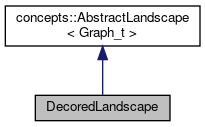
\includegraphics[width=226pt]{class_decored_landscape__coll__graph}
\end{center}
\end{figure}
\subsection*{Public Member Functions}
\begin{DoxyCompactItemize}
\item 
\hyperlink{class_decored_landscape_ae7ba2eb4a09b153b238f22fcb33b5260}{Decored\+Landscape} (const \hyperlink{pl__reff_8cpp_a65aea14f39d53b24df9910d54216d620}{Graph\+\_\+t} \&original\+\_\+graph, const Graph\+\_\+t\+::\+Node\+Map$<$ double $>$ \&original\+\_\+quality\+Map, const Graph\+\_\+t\+::\+Arc\+Map$<$ double $>$ \&original\+\_\+probability\+Map, const \hyperlink{classconcepts_1_1_abstract_landscape_a8432d7dff7edc5a5cbc524592b411f8a}{Coords\+Map} \&coords\+Map)
\item 
\hyperlink{class_decored_landscape_a501bfb6656d735d8a564ea4c0aa6ccfd}{Decored\+Landscape} (const \hyperlink{class_landscape}{Landscape} \&landscape)
\item 
\hyperlink{class_decored_landscape_a5fcaa5685a1296f29b382fcde0f6ee0e}{$\sim$\+Decored\+Landscape} ()
\item 
const \hyperlink{classconcepts_1_1_abstract_landscape_ab1988ca4ff36329c45af21e76046903d}{Graph} \& \hyperlink{class_decored_landscape_ae0cf946d7f221b0b7cbf89a645806d74}{get\+Network} () const
\item 
const \hyperlink{classconcepts_1_1_abstract_landscape_aab540b896ac9b7a7a5783f2a78f304ad}{Quality\+Map} \& \hyperlink{class_decored_landscape_a0493646916af886d3d0404760c3d5e4e}{get\+Quality\+Map} () const
\item 
const \hyperlink{classconcepts_1_1_abstract_landscape_a8432d7dff7edc5a5cbc524592b411f8a}{Coords\+Map} \& \hyperlink{class_decored_landscape_a66994174c58cad04d5fa75cb24ef2772}{get\+Coords\+Map} () const
\item 
const \hyperlink{classconcepts_1_1_abstract_landscape_ae90ffb759facff21b29e646539352182}{Probability\+Map} \& \hyperlink{class_decored_landscape_afdc878affae92d7c671f1e0f87223ee0}{get\+Probability\+Map} () const
\item 
const double \& \hyperlink{class_decored_landscape_a5bfb2c9f5ef7e7c760d8804d0ffd9d9b}{get\+Quality} (Graph\+\_\+t\+::\+Node u) const
\item 
const \hyperlink{abstract__landscape_8hpp_a9c14bcba65b035519a9c98f1eb1babbe}{Point} \& \hyperlink{class_decored_landscape_a45685d1bf37d032f1793f885eaf4e80c}{get\+Coords} (Graph\+\_\+t\+::\+Node u) const
\item 
const double \& \hyperlink{class_decored_landscape_a09b5ea325960556e0a834a53a7b53000}{get\+Probability} (Graph\+\_\+t\+::\+Arc a) const
\item 
double \& \hyperlink{class_decored_landscape_a2c6557a008e3b8a6d93bf307a71a1b33}{get\+Quality\+Ref} (Graph\+\_\+t\+::\+Node u)
\item 
double \& \hyperlink{class_decored_landscape_a16bd4da5d77b804cecb864c11770a344}{get\+Probability\+Ref} (Graph\+\_\+t\+::\+Arc a)
\item 
void \hyperlink{class_decored_landscape_a76d4269a5c48601b0a31dbf91b3cbafe}{set\+Quality} (Graph\+\_\+t\+::\+Node u, double v)
\item 
void \hyperlink{class_decored_landscape_a53063f0f592b1cd00c3456fd40722c53}{set\+Probability} (Graph\+\_\+t\+::\+Arc e, double v)
\item 
const double \& \hyperlink{class_decored_landscape_a136c0034f2953fd59332d73b6eb17b19}{get\+Original\+Quality} (Graph\+\_\+t\+::\+Node u) const
\begin{DoxyCompactList}\small\item\em Get the original quality of specified node. \end{DoxyCompactList}\item 
const double \& \hyperlink{class_decored_landscape_af45ece8a6787d42c0d60c90de913b9f5}{get\+Original\+Probability} (Graph\+\_\+t\+::\+Arc a) const
\begin{DoxyCompactList}\small\item\em Get the original difficulty of specified arc. \end{DoxyCompactList}\item 
void \hyperlink{class_decored_landscape_a9acf573f999cbf3e96fb567a89d02a1b}{reset} ()
\begin{DoxyCompactList}\small\item\em Resets the weights of the landscape to its original ones. \end{DoxyCompactList}\item 
void \hyperlink{class_decored_landscape_a4613b09e1b8d817095dd486f9c1224b8}{apply} (const \hyperlink{class_restoration_plan_1_1_option}{Restoration\+Plan\+::\+Option} $\ast$option, double coef=1.\+0)
\begin{DoxyCompactList}\small\item\em Decorates the landscape by applying the specified resotoration option. \end{DoxyCompactList}\end{DoxyCompactItemize}
\subsection*{Additional Inherited Members}


\subsection{Detailed Description}
Class that represent an decored landscape. 

This class represent a decored landscape. That is a modification of the weights of a reference landscape. 

\subsection{Constructor \& Destructor Documentation}
\mbox{\Hypertarget{class_decored_landscape_ae7ba2eb4a09b153b238f22fcb33b5260}\label{class_decored_landscape_ae7ba2eb4a09b153b238f22fcb33b5260}} 
\index{Decored\+Landscape@{Decored\+Landscape}!Decored\+Landscape@{Decored\+Landscape}}
\index{Decored\+Landscape@{Decored\+Landscape}!Decored\+Landscape@{Decored\+Landscape}}
\subsubsection{\texorpdfstring{Decored\+Landscape()}{DecoredLandscape()}\hspace{0.1cm}{\footnotesize\ttfamily [1/2]}}
{\footnotesize\ttfamily Decored\+Landscape\+::\+Decored\+Landscape (\begin{DoxyParamCaption}\item[{const \hyperlink{pl__reff_8cpp_a65aea14f39d53b24df9910d54216d620}{Graph\+\_\+t} \&}]{original\+\_\+graph,  }\item[{const Graph\+\_\+t\+::\+Node\+Map$<$ double $>$ \&}]{original\+\_\+quality\+Map,  }\item[{const Graph\+\_\+t\+::\+Arc\+Map$<$ double $>$ \&}]{original\+\_\+probability\+Map,  }\item[{const \hyperlink{classconcepts_1_1_abstract_landscape_a8432d7dff7edc5a5cbc524592b411f8a}{Coords\+Map} \&}]{coords\+Map }\end{DoxyParamCaption})}

\mbox{\Hypertarget{class_decored_landscape_a501bfb6656d735d8a564ea4c0aa6ccfd}\label{class_decored_landscape_a501bfb6656d735d8a564ea4c0aa6ccfd}} 
\index{Decored\+Landscape@{Decored\+Landscape}!Decored\+Landscape@{Decored\+Landscape}}
\index{Decored\+Landscape@{Decored\+Landscape}!Decored\+Landscape@{Decored\+Landscape}}
\subsubsection{\texorpdfstring{Decored\+Landscape()}{DecoredLandscape()}\hspace{0.1cm}{\footnotesize\ttfamily [2/2]}}
{\footnotesize\ttfamily Decored\+Landscape\+::\+Decored\+Landscape (\begin{DoxyParamCaption}\item[{const \hyperlink{class_landscape}{Landscape} \&}]{landscape }\end{DoxyParamCaption})}

\mbox{\Hypertarget{class_decored_landscape_a5fcaa5685a1296f29b382fcde0f6ee0e}\label{class_decored_landscape_a5fcaa5685a1296f29b382fcde0f6ee0e}} 
\index{Decored\+Landscape@{Decored\+Landscape}!````~Decored\+Landscape@{$\sim$\+Decored\+Landscape}}
\index{````~Decored\+Landscape@{$\sim$\+Decored\+Landscape}!Decored\+Landscape@{Decored\+Landscape}}
\subsubsection{\texorpdfstring{$\sim$\+Decored\+Landscape()}{~DecoredLandscape()}}
{\footnotesize\ttfamily Decored\+Landscape\+::$\sim$\+Decored\+Landscape (\begin{DoxyParamCaption}{ }\end{DoxyParamCaption})}



\subsection{Member Function Documentation}
\mbox{\Hypertarget{class_decored_landscape_a4613b09e1b8d817095dd486f9c1224b8}\label{class_decored_landscape_a4613b09e1b8d817095dd486f9c1224b8}} 
\index{Decored\+Landscape@{Decored\+Landscape}!apply@{apply}}
\index{apply@{apply}!Decored\+Landscape@{Decored\+Landscape}}
\subsubsection{\texorpdfstring{apply()}{apply()}}
{\footnotesize\ttfamily void Decored\+Landscape\+::apply (\begin{DoxyParamCaption}\item[{const \hyperlink{class_restoration_plan_1_1_option}{Restoration\+Plan\+::\+Option} $\ast$}]{option,  }\item[{double}]{coef = {\ttfamily 1.0} }\end{DoxyParamCaption})}



Decorates the landscape by applying the specified resotoration option. 

Enhances the propoerties of the elements concerned by the specified restoration option according to a coefficient.


\begin{DoxyParams}{Parameters}
{\em option} & \\
\hline
{\em coef} & \+: \$\mbox{[}0,1\mbox{]}\$, the portion of option to consider \\
\hline
\end{DoxyParams}
\mbox{\Hypertarget{class_decored_landscape_a45685d1bf37d032f1793f885eaf4e80c}\label{class_decored_landscape_a45685d1bf37d032f1793f885eaf4e80c}} 
\index{Decored\+Landscape@{Decored\+Landscape}!get\+Coords@{get\+Coords}}
\index{get\+Coords@{get\+Coords}!Decored\+Landscape@{Decored\+Landscape}}
\subsubsection{\texorpdfstring{get\+Coords()}{getCoords()}}
{\footnotesize\ttfamily const \hyperlink{abstract__landscape_8hpp_a9c14bcba65b035519a9c98f1eb1babbe}{Point} \& Decored\+Landscape\+::get\+Coords (\begin{DoxyParamCaption}\item[{Graph\+\_\+t\+::\+Node}]{u }\end{DoxyParamCaption}) const}

\mbox{\Hypertarget{class_decored_landscape_a66994174c58cad04d5fa75cb24ef2772}\label{class_decored_landscape_a66994174c58cad04d5fa75cb24ef2772}} 
\index{Decored\+Landscape@{Decored\+Landscape}!get\+Coords\+Map@{get\+Coords\+Map}}
\index{get\+Coords\+Map@{get\+Coords\+Map}!Decored\+Landscape@{Decored\+Landscape}}
\subsubsection{\texorpdfstring{get\+Coords\+Map()}{getCoordsMap()}}
{\footnotesize\ttfamily const \hyperlink{classconcepts_1_1_abstract_landscape_a8432d7dff7edc5a5cbc524592b411f8a}{Decored\+Landscape\+::\+Coords\+Map} \& Decored\+Landscape\+::get\+Coords\+Map (\begin{DoxyParamCaption}{ }\end{DoxyParamCaption}) const\hspace{0.3cm}{\ttfamily [virtual]}}



Implements \hyperlink{classconcepts_1_1_abstract_landscape_a5005b0254f3c5aa0ed8505386fca92b3}{concepts\+::\+Abstract\+Landscape$<$ Graph\+\_\+t $>$}.

\mbox{\Hypertarget{class_decored_landscape_ae0cf946d7f221b0b7cbf89a645806d74}\label{class_decored_landscape_ae0cf946d7f221b0b7cbf89a645806d74}} 
\index{Decored\+Landscape@{Decored\+Landscape}!get\+Network@{get\+Network}}
\index{get\+Network@{get\+Network}!Decored\+Landscape@{Decored\+Landscape}}
\subsubsection{\texorpdfstring{get\+Network()}{getNetwork()}}
{\footnotesize\ttfamily const \hyperlink{pl__reff_8cpp_a65aea14f39d53b24df9910d54216d620}{Graph\+\_\+t} \& Decored\+Landscape\+::get\+Network (\begin{DoxyParamCaption}{ }\end{DoxyParamCaption}) const\hspace{0.3cm}{\ttfamily [virtual]}}



Implements \hyperlink{classconcepts_1_1_abstract_landscape_a7ed478b62e37cad9a22bed3adedf07c5}{concepts\+::\+Abstract\+Landscape$<$ Graph\+\_\+t $>$}.

\mbox{\Hypertarget{class_decored_landscape_af45ece8a6787d42c0d60c90de913b9f5}\label{class_decored_landscape_af45ece8a6787d42c0d60c90de913b9f5}} 
\index{Decored\+Landscape@{Decored\+Landscape}!get\+Original\+Probability@{get\+Original\+Probability}}
\index{get\+Original\+Probability@{get\+Original\+Probability}!Decored\+Landscape@{Decored\+Landscape}}
\subsubsection{\texorpdfstring{get\+Original\+Probability()}{getOriginalProbability()}}
{\footnotesize\ttfamily const double \& Decored\+Landscape\+::get\+Original\+Probability (\begin{DoxyParamCaption}\item[{Graph\+\_\+t\+::\+Arc}]{a }\end{DoxyParamCaption}) const}



Get the original difficulty of specified arc. 


\begin{DoxyParams}{Parameters}
{\em u} & \\
\hline
\end{DoxyParams}
\begin{DoxyReturn}{Returns}
const double\& 
\end{DoxyReturn}
\mbox{\Hypertarget{class_decored_landscape_a136c0034f2953fd59332d73b6eb17b19}\label{class_decored_landscape_a136c0034f2953fd59332d73b6eb17b19}} 
\index{Decored\+Landscape@{Decored\+Landscape}!get\+Original\+Quality@{get\+Original\+Quality}}
\index{get\+Original\+Quality@{get\+Original\+Quality}!Decored\+Landscape@{Decored\+Landscape}}
\subsubsection{\texorpdfstring{get\+Original\+Quality()}{getOriginalQuality()}}
{\footnotesize\ttfamily const double \& Decored\+Landscape\+::get\+Original\+Quality (\begin{DoxyParamCaption}\item[{Graph\+\_\+t\+::\+Node}]{u }\end{DoxyParamCaption}) const}



Get the original quality of specified node. 


\begin{DoxyParams}{Parameters}
{\em u} & \\
\hline
\end{DoxyParams}
\begin{DoxyReturn}{Returns}
const double\& 
\end{DoxyReturn}
\mbox{\Hypertarget{class_decored_landscape_a09b5ea325960556e0a834a53a7b53000}\label{class_decored_landscape_a09b5ea325960556e0a834a53a7b53000}} 
\index{Decored\+Landscape@{Decored\+Landscape}!get\+Probability@{get\+Probability}}
\index{get\+Probability@{get\+Probability}!Decored\+Landscape@{Decored\+Landscape}}
\subsubsection{\texorpdfstring{get\+Probability()}{getProbability()}}
{\footnotesize\ttfamily const double \& Decored\+Landscape\+::get\+Probability (\begin{DoxyParamCaption}\item[{Graph\+\_\+t\+::\+Arc}]{a }\end{DoxyParamCaption}) const}

\mbox{\Hypertarget{class_decored_landscape_afdc878affae92d7c671f1e0f87223ee0}\label{class_decored_landscape_afdc878affae92d7c671f1e0f87223ee0}} 
\index{Decored\+Landscape@{Decored\+Landscape}!get\+Probability\+Map@{get\+Probability\+Map}}
\index{get\+Probability\+Map@{get\+Probability\+Map}!Decored\+Landscape@{Decored\+Landscape}}
\subsubsection{\texorpdfstring{get\+Probability\+Map()}{getProbabilityMap()}}
{\footnotesize\ttfamily const \hyperlink{classconcepts_1_1_abstract_landscape_ae90ffb759facff21b29e646539352182}{Decored\+Landscape\+::\+Probability\+Map} \& Decored\+Landscape\+::get\+Probability\+Map (\begin{DoxyParamCaption}{ }\end{DoxyParamCaption}) const\hspace{0.3cm}{\ttfamily [virtual]}}



Implements \hyperlink{classconcepts_1_1_abstract_landscape_a4ecbe83965a5266a3a2fa14e201c5871}{concepts\+::\+Abstract\+Landscape$<$ Graph\+\_\+t $>$}.

\mbox{\Hypertarget{class_decored_landscape_a16bd4da5d77b804cecb864c11770a344}\label{class_decored_landscape_a16bd4da5d77b804cecb864c11770a344}} 
\index{Decored\+Landscape@{Decored\+Landscape}!get\+Probability\+Ref@{get\+Probability\+Ref}}
\index{get\+Probability\+Ref@{get\+Probability\+Ref}!Decored\+Landscape@{Decored\+Landscape}}
\subsubsection{\texorpdfstring{get\+Probability\+Ref()}{getProbabilityRef()}}
{\footnotesize\ttfamily double \& Decored\+Landscape\+::get\+Probability\+Ref (\begin{DoxyParamCaption}\item[{Graph\+\_\+t\+::\+Arc}]{a }\end{DoxyParamCaption})}

\mbox{\Hypertarget{class_decored_landscape_a5bfb2c9f5ef7e7c760d8804d0ffd9d9b}\label{class_decored_landscape_a5bfb2c9f5ef7e7c760d8804d0ffd9d9b}} 
\index{Decored\+Landscape@{Decored\+Landscape}!get\+Quality@{get\+Quality}}
\index{get\+Quality@{get\+Quality}!Decored\+Landscape@{Decored\+Landscape}}
\subsubsection{\texorpdfstring{get\+Quality()}{getQuality()}}
{\footnotesize\ttfamily const double \& Decored\+Landscape\+::get\+Quality (\begin{DoxyParamCaption}\item[{Graph\+\_\+t\+::\+Node}]{u }\end{DoxyParamCaption}) const}

\mbox{\Hypertarget{class_decored_landscape_a0493646916af886d3d0404760c3d5e4e}\label{class_decored_landscape_a0493646916af886d3d0404760c3d5e4e}} 
\index{Decored\+Landscape@{Decored\+Landscape}!get\+Quality\+Map@{get\+Quality\+Map}}
\index{get\+Quality\+Map@{get\+Quality\+Map}!Decored\+Landscape@{Decored\+Landscape}}
\subsubsection{\texorpdfstring{get\+Quality\+Map()}{getQualityMap()}}
{\footnotesize\ttfamily const \hyperlink{classconcepts_1_1_abstract_landscape_aab540b896ac9b7a7a5783f2a78f304ad}{Decored\+Landscape\+::\+Quality\+Map} \& Decored\+Landscape\+::get\+Quality\+Map (\begin{DoxyParamCaption}{ }\end{DoxyParamCaption}) const\hspace{0.3cm}{\ttfamily [virtual]}}



Implements \hyperlink{classconcepts_1_1_abstract_landscape_ab0ff4aa5ac8d95d9207e32582e3e95f2}{concepts\+::\+Abstract\+Landscape$<$ Graph\+\_\+t $>$}.

\mbox{\Hypertarget{class_decored_landscape_a2c6557a008e3b8a6d93bf307a71a1b33}\label{class_decored_landscape_a2c6557a008e3b8a6d93bf307a71a1b33}} 
\index{Decored\+Landscape@{Decored\+Landscape}!get\+Quality\+Ref@{get\+Quality\+Ref}}
\index{get\+Quality\+Ref@{get\+Quality\+Ref}!Decored\+Landscape@{Decored\+Landscape}}
\subsubsection{\texorpdfstring{get\+Quality\+Ref()}{getQualityRef()}}
{\footnotesize\ttfamily double \& Decored\+Landscape\+::get\+Quality\+Ref (\begin{DoxyParamCaption}\item[{Graph\+\_\+t\+::\+Node}]{u }\end{DoxyParamCaption})}

\mbox{\Hypertarget{class_decored_landscape_a9acf573f999cbf3e96fb567a89d02a1b}\label{class_decored_landscape_a9acf573f999cbf3e96fb567a89d02a1b}} 
\index{Decored\+Landscape@{Decored\+Landscape}!reset@{reset}}
\index{reset@{reset}!Decored\+Landscape@{Decored\+Landscape}}
\subsubsection{\texorpdfstring{reset()}{reset()}}
{\footnotesize\ttfamily void Decored\+Landscape\+::reset (\begin{DoxyParamCaption}{ }\end{DoxyParamCaption})}



Resets the weights of the landscape to its original ones. 

\mbox{\Hypertarget{class_decored_landscape_a53063f0f592b1cd00c3456fd40722c53}\label{class_decored_landscape_a53063f0f592b1cd00c3456fd40722c53}} 
\index{Decored\+Landscape@{Decored\+Landscape}!set\+Probability@{set\+Probability}}
\index{set\+Probability@{set\+Probability}!Decored\+Landscape@{Decored\+Landscape}}
\subsubsection{\texorpdfstring{set\+Probability()}{setProbability()}}
{\footnotesize\ttfamily void Decored\+Landscape\+::set\+Probability (\begin{DoxyParamCaption}\item[{Graph\+\_\+t\+::\+Arc}]{e,  }\item[{double}]{v }\end{DoxyParamCaption})}

\mbox{\Hypertarget{class_decored_landscape_a76d4269a5c48601b0a31dbf91b3cbafe}\label{class_decored_landscape_a76d4269a5c48601b0a31dbf91b3cbafe}} 
\index{Decored\+Landscape@{Decored\+Landscape}!set\+Quality@{set\+Quality}}
\index{set\+Quality@{set\+Quality}!Decored\+Landscape@{Decored\+Landscape}}
\subsubsection{\texorpdfstring{set\+Quality()}{setQuality()}}
{\footnotesize\ttfamily void Decored\+Landscape\+::set\+Quality (\begin{DoxyParamCaption}\item[{Graph\+\_\+t\+::\+Node}]{u,  }\item[{double}]{v }\end{DoxyParamCaption})}



The documentation for this class was generated from the following files\+:\begin{DoxyCompactItemize}
\item 
/home/plaiseek/\+Projects/landscape\+\_\+opt\+\_\+cpp/include/landscape/\hyperlink{decored__landscape_8hpp}{decored\+\_\+landscape.\+hpp}\item 
/home/plaiseek/\+Projects/landscape\+\_\+opt\+\_\+cpp/src/landscape/\hyperlink{decored__landscape_8cpp}{decored\+\_\+landscape.\+cpp}\end{DoxyCompactItemize}

\hypertarget{structlemon_1_1_dijkstra_multiplicative_operation_traits}{}\section{lemon\+:\+:Dijkstra\+Multiplicative\+Operation\+Traits$<$ V $>$ Struct Template Reference}
\label{structlemon_1_1_dijkstra_multiplicative_operation_traits}\index{lemon\+::\+Dijkstra\+Multiplicative\+Operation\+Traits$<$ V $>$@{lemon\+::\+Dijkstra\+Multiplicative\+Operation\+Traits$<$ V $>$}}


Multiplicative operation traits for the Dijkstra algorithm class.  




{\ttfamily \#include $<$multiplicative\+\_\+dijkstra.\+h$>$}

\subsection*{Public Types}
\begin{DoxyCompactItemize}
\item 
typedef V \hyperlink{structlemon_1_1_dijkstra_multiplicative_operation_traits_a8832632b11125d59eedb238160bc1554}{Value}
\end{DoxyCompactItemize}
\subsection*{Static Public Member Functions}
\begin{DoxyCompactItemize}
\item 
static \hyperlink{structlemon_1_1_dijkstra_multiplicative_operation_traits_a8832632b11125d59eedb238160bc1554}{Value} \hyperlink{structlemon_1_1_dijkstra_multiplicative_operation_traits_a42a0a16398e1548efd8ffb3616b13866}{zero} ()
\item 
static \hyperlink{structlemon_1_1_dijkstra_multiplicative_operation_traits_a8832632b11125d59eedb238160bc1554}{Value} \hyperlink{structlemon_1_1_dijkstra_multiplicative_operation_traits_a5b8190dbafe5ad4fa70098dcc876c183}{plus} (const \hyperlink{structlemon_1_1_dijkstra_multiplicative_operation_traits_a8832632b11125d59eedb238160bc1554}{Value} \&left, const \hyperlink{structlemon_1_1_dijkstra_multiplicative_operation_traits_a8832632b11125d59eedb238160bc1554}{Value} \&right)
\item 
static bool \hyperlink{structlemon_1_1_dijkstra_multiplicative_operation_traits_a0e6d5f836763e814cb562d7f5e5be67f}{less} (const \hyperlink{structlemon_1_1_dijkstra_multiplicative_operation_traits_a8832632b11125d59eedb238160bc1554}{Value} \&left, const \hyperlink{structlemon_1_1_dijkstra_multiplicative_operation_traits_a8832632b11125d59eedb238160bc1554}{Value} \&right)
\end{DoxyCompactItemize}


\subsection{Detailed Description}
\subsubsection*{template$<$typename V$>$\newline
struct lemon\+::\+Dijkstra\+Multiplicative\+Operation\+Traits$<$ V $>$}

Multiplicative operation traits for the Dijkstra algorithm class. 

This operation traits class defines all computational operations and constants which are used in the multiplicative version of Dijkstra algorithm.


\begin{DoxyTemplParams}{Template Parameters}
{\em V} & \\
\hline
\end{DoxyTemplParams}


\subsection{Member Typedef Documentation}
\mbox{\Hypertarget{structlemon_1_1_dijkstra_multiplicative_operation_traits_a8832632b11125d59eedb238160bc1554}\label{structlemon_1_1_dijkstra_multiplicative_operation_traits_a8832632b11125d59eedb238160bc1554}} 
\index{lemon\+::\+Dijkstra\+Multiplicative\+Operation\+Traits@{lemon\+::\+Dijkstra\+Multiplicative\+Operation\+Traits}!Value@{Value}}
\index{Value@{Value}!lemon\+::\+Dijkstra\+Multiplicative\+Operation\+Traits@{lemon\+::\+Dijkstra\+Multiplicative\+Operation\+Traits}}
\subsubsection{\texorpdfstring{Value}{Value}}
{\footnotesize\ttfamily template$<$typename V $>$ \\
typedef V \hyperlink{structlemon_1_1_dijkstra_multiplicative_operation_traits}{lemon\+::\+Dijkstra\+Multiplicative\+Operation\+Traits}$<$ V $>$\+::\hyperlink{structlemon_1_1_dijkstra_multiplicative_operation_traits_a8832632b11125d59eedb238160bc1554}{Value}}



\subsection{Member Function Documentation}
\mbox{\Hypertarget{structlemon_1_1_dijkstra_multiplicative_operation_traits_a0e6d5f836763e814cb562d7f5e5be67f}\label{structlemon_1_1_dijkstra_multiplicative_operation_traits_a0e6d5f836763e814cb562d7f5e5be67f}} 
\index{lemon\+::\+Dijkstra\+Multiplicative\+Operation\+Traits@{lemon\+::\+Dijkstra\+Multiplicative\+Operation\+Traits}!less@{less}}
\index{less@{less}!lemon\+::\+Dijkstra\+Multiplicative\+Operation\+Traits@{lemon\+::\+Dijkstra\+Multiplicative\+Operation\+Traits}}
\subsubsection{\texorpdfstring{less()}{less()}}
{\footnotesize\ttfamily template$<$typename V $>$ \\
static bool \hyperlink{structlemon_1_1_dijkstra_multiplicative_operation_traits}{lemon\+::\+Dijkstra\+Multiplicative\+Operation\+Traits}$<$ V $>$\+::less (\begin{DoxyParamCaption}\item[{const \hyperlink{structlemon_1_1_dijkstra_multiplicative_operation_traits_a8832632b11125d59eedb238160bc1554}{Value} \&}]{left,  }\item[{const \hyperlink{structlemon_1_1_dijkstra_multiplicative_operation_traits_a8832632b11125d59eedb238160bc1554}{Value} \&}]{right }\end{DoxyParamCaption})\hspace{0.3cm}{\ttfamily [inline]}, {\ttfamily [static]}}

\mbox{\Hypertarget{structlemon_1_1_dijkstra_multiplicative_operation_traits_a5b8190dbafe5ad4fa70098dcc876c183}\label{structlemon_1_1_dijkstra_multiplicative_operation_traits_a5b8190dbafe5ad4fa70098dcc876c183}} 
\index{lemon\+::\+Dijkstra\+Multiplicative\+Operation\+Traits@{lemon\+::\+Dijkstra\+Multiplicative\+Operation\+Traits}!plus@{plus}}
\index{plus@{plus}!lemon\+::\+Dijkstra\+Multiplicative\+Operation\+Traits@{lemon\+::\+Dijkstra\+Multiplicative\+Operation\+Traits}}
\subsubsection{\texorpdfstring{plus()}{plus()}}
{\footnotesize\ttfamily template$<$typename V $>$ \\
static \hyperlink{structlemon_1_1_dijkstra_multiplicative_operation_traits_a8832632b11125d59eedb238160bc1554}{Value} \hyperlink{structlemon_1_1_dijkstra_multiplicative_operation_traits}{lemon\+::\+Dijkstra\+Multiplicative\+Operation\+Traits}$<$ V $>$\+::plus (\begin{DoxyParamCaption}\item[{const \hyperlink{structlemon_1_1_dijkstra_multiplicative_operation_traits_a8832632b11125d59eedb238160bc1554}{Value} \&}]{left,  }\item[{const \hyperlink{structlemon_1_1_dijkstra_multiplicative_operation_traits_a8832632b11125d59eedb238160bc1554}{Value} \&}]{right }\end{DoxyParamCaption})\hspace{0.3cm}{\ttfamily [inline]}, {\ttfamily [static]}}

\mbox{\Hypertarget{structlemon_1_1_dijkstra_multiplicative_operation_traits_a42a0a16398e1548efd8ffb3616b13866}\label{structlemon_1_1_dijkstra_multiplicative_operation_traits_a42a0a16398e1548efd8ffb3616b13866}} 
\index{lemon\+::\+Dijkstra\+Multiplicative\+Operation\+Traits@{lemon\+::\+Dijkstra\+Multiplicative\+Operation\+Traits}!zero@{zero}}
\index{zero@{zero}!lemon\+::\+Dijkstra\+Multiplicative\+Operation\+Traits@{lemon\+::\+Dijkstra\+Multiplicative\+Operation\+Traits}}
\subsubsection{\texorpdfstring{zero()}{zero()}}
{\footnotesize\ttfamily template$<$typename V $>$ \\
static \hyperlink{structlemon_1_1_dijkstra_multiplicative_operation_traits_a8832632b11125d59eedb238160bc1554}{Value} \hyperlink{structlemon_1_1_dijkstra_multiplicative_operation_traits}{lemon\+::\+Dijkstra\+Multiplicative\+Operation\+Traits}$<$ V $>$\+::zero (\begin{DoxyParamCaption}{ }\end{DoxyParamCaption})\hspace{0.3cm}{\ttfamily [inline]}, {\ttfamily [static]}}



The documentation for this struct was generated from the following file\+:\begin{DoxyCompactItemize}
\item 
/home/plaiseek/\+Projects/landscape\+\_\+opt\+\_\+cpp/include/algorithms/\hyperlink{multiplicative__dijkstra_8h}{multiplicative\+\_\+dijkstra.\+h}\end{DoxyCompactItemize}

\hypertarget{structlemon_1_1_dijkstra_multiplicative_traits}{}\section{lemon\+:\+:Dijkstra\+Multiplicative\+Traits$<$ GR, L\+EN $>$ Struct Template Reference}
\label{structlemon_1_1_dijkstra_multiplicative_traits}\index{lemon\+::\+Dijkstra\+Multiplicative\+Traits$<$ G\+R, L\+E\+N $>$@{lemon\+::\+Dijkstra\+Multiplicative\+Traits$<$ G\+R, L\+E\+N $>$}}


Multiplicative traits class of Dijkstra class.  




{\ttfamily \#include $<$multiplicative\+\_\+dijkstra.\+h$>$}

\subsection*{Public Types}
\begin{DoxyCompactItemize}
\item 
typedef GR \hyperlink{structlemon_1_1_dijkstra_multiplicative_traits_a3ad6d100e3d5d097aaaac8e5733ce3a3}{Digraph}
\item 
typedef L\+EN \hyperlink{structlemon_1_1_dijkstra_multiplicative_traits_a71b3ebdd887bad38c0a80bdee34204b7}{Length\+Map}
\item 
typedef L\+E\+N\+::\+Value \hyperlink{structlemon_1_1_dijkstra_multiplicative_traits_a6e84de41f8b2d8c17974487766c465cf}{Value}
\item 
typedef \hyperlink{structlemon_1_1_dijkstra_multiplicative_operation_traits}{Dijkstra\+Multiplicative\+Operation\+Traits}$<$ \hyperlink{structlemon_1_1_dijkstra_multiplicative_traits_a6e84de41f8b2d8c17974487766c465cf}{Value} $>$ \hyperlink{structlemon_1_1_dijkstra_multiplicative_traits_affb2683da11abbf82ff4e5004046c53d}{Operation\+Traits}
\item 
typedef Digraph\+::template Node\+Map$<$ int $>$ \hyperlink{structlemon_1_1_dijkstra_multiplicative_traits_a6cf2d1691e812bc74967eb6a96bb2110}{Heap\+Cross\+Ref}
\item 
typedef Bin\+Heap$<$ typename L\+E\+N\+::\+Value, \hyperlink{structlemon_1_1_dijkstra_multiplicative_traits_a6cf2d1691e812bc74967eb6a96bb2110}{Heap\+Cross\+Ref}, std\+::greater$<$ \hyperlink{structlemon_1_1_dijkstra_multiplicative_traits_a6e84de41f8b2d8c17974487766c465cf}{Value} $>$ $>$ \hyperlink{structlemon_1_1_dijkstra_multiplicative_traits_ac1f01fa6da75e3af4ca1baabc6be06b8}{Heap}
\item 
typedef Digraph\+::template Node\+Map$<$ typename Digraph\+::\+Arc $>$ \hyperlink{structlemon_1_1_dijkstra_multiplicative_traits_aa69cc345580a8a6619b0add76aae29e0}{Pred\+Map}
\item 
typedef Null\+Map$<$ typename Digraph\+::\+Node, bool $>$ \hyperlink{structlemon_1_1_dijkstra_multiplicative_traits_a48325a83c92b35041eac397cf1728375}{Processed\+Map}
\item 
typedef Digraph\+::template Node\+Map$<$ typename L\+E\+N\+::\+Value $>$ \hyperlink{structlemon_1_1_dijkstra_multiplicative_traits_a2bc3b74c3467b4762e2ac57ea68ef78e}{Dist\+Map}
\end{DoxyCompactItemize}
\subsection*{Static Public Member Functions}
\begin{DoxyCompactItemize}
\item 
static \hyperlink{structlemon_1_1_dijkstra_multiplicative_traits_a6cf2d1691e812bc74967eb6a96bb2110}{Heap\+Cross\+Ref} $\ast$ \hyperlink{structlemon_1_1_dijkstra_multiplicative_traits_aeb8014da9f6368243c538a6a2841d08c}{create\+Heap\+Cross\+Ref} (const \hyperlink{structlemon_1_1_dijkstra_multiplicative_traits_a3ad6d100e3d5d097aaaac8e5733ce3a3}{Digraph} \&g)
\item 
static \hyperlink{structlemon_1_1_dijkstra_multiplicative_traits_ac1f01fa6da75e3af4ca1baabc6be06b8}{Heap} $\ast$ \hyperlink{structlemon_1_1_dijkstra_multiplicative_traits_a395fcb4c11535249168133c009bbf8e4}{create\+Heap} (\hyperlink{structlemon_1_1_dijkstra_multiplicative_traits_a6cf2d1691e812bc74967eb6a96bb2110}{Heap\+Cross\+Ref} \&r)
\item 
static \hyperlink{structlemon_1_1_dijkstra_multiplicative_traits_aa69cc345580a8a6619b0add76aae29e0}{Pred\+Map} $\ast$ \hyperlink{structlemon_1_1_dijkstra_multiplicative_traits_a898d963d49216f0f90870442fbce38d5}{create\+Pred\+Map} (const \hyperlink{structlemon_1_1_dijkstra_multiplicative_traits_a3ad6d100e3d5d097aaaac8e5733ce3a3}{Digraph} \&g)
\item 
static \hyperlink{structlemon_1_1_dijkstra_multiplicative_traits_a48325a83c92b35041eac397cf1728375}{Processed\+Map} $\ast$ \hyperlink{structlemon_1_1_dijkstra_multiplicative_traits_a7ecae716219efe0cafab361a597f90e3}{create\+Processed\+Map} (const \hyperlink{structlemon_1_1_dijkstra_multiplicative_traits_a3ad6d100e3d5d097aaaac8e5733ce3a3}{Digraph} \&)
\item 
static \hyperlink{structlemon_1_1_dijkstra_multiplicative_traits_a2bc3b74c3467b4762e2ac57ea68ef78e}{Dist\+Map} $\ast$ \hyperlink{structlemon_1_1_dijkstra_multiplicative_traits_acd6a683858eba3181c8c51a28b5fa68d}{create\+Dist\+Map} (const \hyperlink{structlemon_1_1_dijkstra_multiplicative_traits_a3ad6d100e3d5d097aaaac8e5733ce3a3}{Digraph} \&g)
\end{DoxyCompactItemize}


\subsection{Detailed Description}
\subsubsection*{template$<$typename GR, typename L\+EN$>$\newline
struct lemon\+::\+Dijkstra\+Multiplicative\+Traits$<$ G\+R, L\+E\+N $>$}

Multiplicative traits class of Dijkstra class. 


\begin{DoxyTemplParams}{Template Parameters}
{\em GR} & The type of the digraph. \\
\hline
{\em L\+EN} & The type of the length map. \\
\hline
\end{DoxyTemplParams}


\subsection{Member Typedef Documentation}
\mbox{\Hypertarget{structlemon_1_1_dijkstra_multiplicative_traits_a3ad6d100e3d5d097aaaac8e5733ce3a3}\label{structlemon_1_1_dijkstra_multiplicative_traits_a3ad6d100e3d5d097aaaac8e5733ce3a3}} 
\index{lemon\+::\+Dijkstra\+Multiplicative\+Traits@{lemon\+::\+Dijkstra\+Multiplicative\+Traits}!Digraph@{Digraph}}
\index{Digraph@{Digraph}!lemon\+::\+Dijkstra\+Multiplicative\+Traits@{lemon\+::\+Dijkstra\+Multiplicative\+Traits}}
\subsubsection{\texorpdfstring{Digraph}{Digraph}}
{\footnotesize\ttfamily template$<$typename GR , typename L\+EN $>$ \\
typedef GR \hyperlink{structlemon_1_1_dijkstra_multiplicative_traits}{lemon\+::\+Dijkstra\+Multiplicative\+Traits}$<$ GR, L\+EN $>$\+::\hyperlink{structlemon_1_1_dijkstra_multiplicative_traits_a3ad6d100e3d5d097aaaac8e5733ce3a3}{Digraph}}

\mbox{\Hypertarget{structlemon_1_1_dijkstra_multiplicative_traits_a2bc3b74c3467b4762e2ac57ea68ef78e}\label{structlemon_1_1_dijkstra_multiplicative_traits_a2bc3b74c3467b4762e2ac57ea68ef78e}} 
\index{lemon\+::\+Dijkstra\+Multiplicative\+Traits@{lemon\+::\+Dijkstra\+Multiplicative\+Traits}!Dist\+Map@{Dist\+Map}}
\index{Dist\+Map@{Dist\+Map}!lemon\+::\+Dijkstra\+Multiplicative\+Traits@{lemon\+::\+Dijkstra\+Multiplicative\+Traits}}
\subsubsection{\texorpdfstring{Dist\+Map}{DistMap}}
{\footnotesize\ttfamily template$<$typename GR , typename L\+EN $>$ \\
typedef Digraph\+::template Node\+Map$<$typename L\+E\+N\+::\+Value$>$ \hyperlink{structlemon_1_1_dijkstra_multiplicative_traits}{lemon\+::\+Dijkstra\+Multiplicative\+Traits}$<$ GR, L\+EN $>$\+::\hyperlink{structlemon_1_1_dijkstra_multiplicative_traits_a2bc3b74c3467b4762e2ac57ea68ef78e}{Dist\+Map}}

\mbox{\Hypertarget{structlemon_1_1_dijkstra_multiplicative_traits_ac1f01fa6da75e3af4ca1baabc6be06b8}\label{structlemon_1_1_dijkstra_multiplicative_traits_ac1f01fa6da75e3af4ca1baabc6be06b8}} 
\index{lemon\+::\+Dijkstra\+Multiplicative\+Traits@{lemon\+::\+Dijkstra\+Multiplicative\+Traits}!Heap@{Heap}}
\index{Heap@{Heap}!lemon\+::\+Dijkstra\+Multiplicative\+Traits@{lemon\+::\+Dijkstra\+Multiplicative\+Traits}}
\subsubsection{\texorpdfstring{Heap}{Heap}}
{\footnotesize\ttfamily template$<$typename GR , typename L\+EN $>$ \\
typedef Bin\+Heap$<$typename L\+E\+N\+::\+Value, \hyperlink{structlemon_1_1_dijkstra_multiplicative_traits_a6cf2d1691e812bc74967eb6a96bb2110}{Heap\+Cross\+Ref}, std\+::greater$<$\hyperlink{structlemon_1_1_dijkstra_multiplicative_traits_a6e84de41f8b2d8c17974487766c465cf}{Value}$>$ $>$ \hyperlink{structlemon_1_1_dijkstra_multiplicative_traits}{lemon\+::\+Dijkstra\+Multiplicative\+Traits}$<$ GR, L\+EN $>$\+::\hyperlink{structlemon_1_1_dijkstra_multiplicative_traits_ac1f01fa6da75e3af4ca1baabc6be06b8}{Heap}}

\mbox{\Hypertarget{structlemon_1_1_dijkstra_multiplicative_traits_a6cf2d1691e812bc74967eb6a96bb2110}\label{structlemon_1_1_dijkstra_multiplicative_traits_a6cf2d1691e812bc74967eb6a96bb2110}} 
\index{lemon\+::\+Dijkstra\+Multiplicative\+Traits@{lemon\+::\+Dijkstra\+Multiplicative\+Traits}!Heap\+Cross\+Ref@{Heap\+Cross\+Ref}}
\index{Heap\+Cross\+Ref@{Heap\+Cross\+Ref}!lemon\+::\+Dijkstra\+Multiplicative\+Traits@{lemon\+::\+Dijkstra\+Multiplicative\+Traits}}
\subsubsection{\texorpdfstring{Heap\+Cross\+Ref}{HeapCrossRef}}
{\footnotesize\ttfamily template$<$typename GR , typename L\+EN $>$ \\
typedef Digraph\+::template Node\+Map$<$int$>$ \hyperlink{structlemon_1_1_dijkstra_multiplicative_traits}{lemon\+::\+Dijkstra\+Multiplicative\+Traits}$<$ GR, L\+EN $>$\+::\hyperlink{structlemon_1_1_dijkstra_multiplicative_traits_a6cf2d1691e812bc74967eb6a96bb2110}{Heap\+Cross\+Ref}}

\mbox{\Hypertarget{structlemon_1_1_dijkstra_multiplicative_traits_a71b3ebdd887bad38c0a80bdee34204b7}\label{structlemon_1_1_dijkstra_multiplicative_traits_a71b3ebdd887bad38c0a80bdee34204b7}} 
\index{lemon\+::\+Dijkstra\+Multiplicative\+Traits@{lemon\+::\+Dijkstra\+Multiplicative\+Traits}!Length\+Map@{Length\+Map}}
\index{Length\+Map@{Length\+Map}!lemon\+::\+Dijkstra\+Multiplicative\+Traits@{lemon\+::\+Dijkstra\+Multiplicative\+Traits}}
\subsubsection{\texorpdfstring{Length\+Map}{LengthMap}}
{\footnotesize\ttfamily template$<$typename GR , typename L\+EN $>$ \\
typedef L\+EN \hyperlink{structlemon_1_1_dijkstra_multiplicative_traits}{lemon\+::\+Dijkstra\+Multiplicative\+Traits}$<$ GR, L\+EN $>$\+::\hyperlink{structlemon_1_1_dijkstra_multiplicative_traits_a71b3ebdd887bad38c0a80bdee34204b7}{Length\+Map}}

\mbox{\Hypertarget{structlemon_1_1_dijkstra_multiplicative_traits_affb2683da11abbf82ff4e5004046c53d}\label{structlemon_1_1_dijkstra_multiplicative_traits_affb2683da11abbf82ff4e5004046c53d}} 
\index{lemon\+::\+Dijkstra\+Multiplicative\+Traits@{lemon\+::\+Dijkstra\+Multiplicative\+Traits}!Operation\+Traits@{Operation\+Traits}}
\index{Operation\+Traits@{Operation\+Traits}!lemon\+::\+Dijkstra\+Multiplicative\+Traits@{lemon\+::\+Dijkstra\+Multiplicative\+Traits}}
\subsubsection{\texorpdfstring{Operation\+Traits}{OperationTraits}}
{\footnotesize\ttfamily template$<$typename GR , typename L\+EN $>$ \\
typedef \hyperlink{structlemon_1_1_dijkstra_multiplicative_operation_traits}{Dijkstra\+Multiplicative\+Operation\+Traits}$<$\hyperlink{structlemon_1_1_dijkstra_multiplicative_traits_a6e84de41f8b2d8c17974487766c465cf}{Value}$>$ \hyperlink{structlemon_1_1_dijkstra_multiplicative_traits}{lemon\+::\+Dijkstra\+Multiplicative\+Traits}$<$ GR, L\+EN $>$\+::\hyperlink{structlemon_1_1_dijkstra_multiplicative_traits_affb2683da11abbf82ff4e5004046c53d}{Operation\+Traits}}

\mbox{\Hypertarget{structlemon_1_1_dijkstra_multiplicative_traits_aa69cc345580a8a6619b0add76aae29e0}\label{structlemon_1_1_dijkstra_multiplicative_traits_aa69cc345580a8a6619b0add76aae29e0}} 
\index{lemon\+::\+Dijkstra\+Multiplicative\+Traits@{lemon\+::\+Dijkstra\+Multiplicative\+Traits}!Pred\+Map@{Pred\+Map}}
\index{Pred\+Map@{Pred\+Map}!lemon\+::\+Dijkstra\+Multiplicative\+Traits@{lemon\+::\+Dijkstra\+Multiplicative\+Traits}}
\subsubsection{\texorpdfstring{Pred\+Map}{PredMap}}
{\footnotesize\ttfamily template$<$typename GR , typename L\+EN $>$ \\
typedef Digraph\+::template Node\+Map$<$typename Digraph\+::\+Arc$>$ \hyperlink{structlemon_1_1_dijkstra_multiplicative_traits}{lemon\+::\+Dijkstra\+Multiplicative\+Traits}$<$ GR, L\+EN $>$\+::\hyperlink{structlemon_1_1_dijkstra_multiplicative_traits_aa69cc345580a8a6619b0add76aae29e0}{Pred\+Map}}

\mbox{\Hypertarget{structlemon_1_1_dijkstra_multiplicative_traits_a48325a83c92b35041eac397cf1728375}\label{structlemon_1_1_dijkstra_multiplicative_traits_a48325a83c92b35041eac397cf1728375}} 
\index{lemon\+::\+Dijkstra\+Multiplicative\+Traits@{lemon\+::\+Dijkstra\+Multiplicative\+Traits}!Processed\+Map@{Processed\+Map}}
\index{Processed\+Map@{Processed\+Map}!lemon\+::\+Dijkstra\+Multiplicative\+Traits@{lemon\+::\+Dijkstra\+Multiplicative\+Traits}}
\subsubsection{\texorpdfstring{Processed\+Map}{ProcessedMap}}
{\footnotesize\ttfamily template$<$typename GR , typename L\+EN $>$ \\
typedef Null\+Map$<$typename Digraph\+::\+Node,bool$>$ \hyperlink{structlemon_1_1_dijkstra_multiplicative_traits}{lemon\+::\+Dijkstra\+Multiplicative\+Traits}$<$ GR, L\+EN $>$\+::\hyperlink{structlemon_1_1_dijkstra_multiplicative_traits_a48325a83c92b35041eac397cf1728375}{Processed\+Map}}

\mbox{\Hypertarget{structlemon_1_1_dijkstra_multiplicative_traits_a6e84de41f8b2d8c17974487766c465cf}\label{structlemon_1_1_dijkstra_multiplicative_traits_a6e84de41f8b2d8c17974487766c465cf}} 
\index{lemon\+::\+Dijkstra\+Multiplicative\+Traits@{lemon\+::\+Dijkstra\+Multiplicative\+Traits}!Value@{Value}}
\index{Value@{Value}!lemon\+::\+Dijkstra\+Multiplicative\+Traits@{lemon\+::\+Dijkstra\+Multiplicative\+Traits}}
\subsubsection{\texorpdfstring{Value}{Value}}
{\footnotesize\ttfamily template$<$typename GR , typename L\+EN $>$ \\
typedef L\+E\+N\+::\+Value \hyperlink{structlemon_1_1_dijkstra_multiplicative_traits}{lemon\+::\+Dijkstra\+Multiplicative\+Traits}$<$ GR, L\+EN $>$\+::\hyperlink{structlemon_1_1_dijkstra_multiplicative_traits_a6e84de41f8b2d8c17974487766c465cf}{Value}}



\subsection{Member Function Documentation}
\mbox{\Hypertarget{structlemon_1_1_dijkstra_multiplicative_traits_acd6a683858eba3181c8c51a28b5fa68d}\label{structlemon_1_1_dijkstra_multiplicative_traits_acd6a683858eba3181c8c51a28b5fa68d}} 
\index{lemon\+::\+Dijkstra\+Multiplicative\+Traits@{lemon\+::\+Dijkstra\+Multiplicative\+Traits}!create\+Dist\+Map@{create\+Dist\+Map}}
\index{create\+Dist\+Map@{create\+Dist\+Map}!lemon\+::\+Dijkstra\+Multiplicative\+Traits@{lemon\+::\+Dijkstra\+Multiplicative\+Traits}}
\subsubsection{\texorpdfstring{create\+Dist\+Map()}{createDistMap()}}
{\footnotesize\ttfamily template$<$typename GR , typename L\+EN $>$ \\
static \hyperlink{structlemon_1_1_dijkstra_multiplicative_traits_a2bc3b74c3467b4762e2ac57ea68ef78e}{Dist\+Map}$\ast$ \hyperlink{structlemon_1_1_dijkstra_multiplicative_traits}{lemon\+::\+Dijkstra\+Multiplicative\+Traits}$<$ GR, L\+EN $>$\+::create\+Dist\+Map (\begin{DoxyParamCaption}\item[{const \hyperlink{structlemon_1_1_dijkstra_multiplicative_traits_a3ad6d100e3d5d097aaaac8e5733ce3a3}{Digraph} \&}]{g }\end{DoxyParamCaption})\hspace{0.3cm}{\ttfamily [inline]}, {\ttfamily [static]}}

\mbox{\Hypertarget{structlemon_1_1_dijkstra_multiplicative_traits_a395fcb4c11535249168133c009bbf8e4}\label{structlemon_1_1_dijkstra_multiplicative_traits_a395fcb4c11535249168133c009bbf8e4}} 
\index{lemon\+::\+Dijkstra\+Multiplicative\+Traits@{lemon\+::\+Dijkstra\+Multiplicative\+Traits}!create\+Heap@{create\+Heap}}
\index{create\+Heap@{create\+Heap}!lemon\+::\+Dijkstra\+Multiplicative\+Traits@{lemon\+::\+Dijkstra\+Multiplicative\+Traits}}
\subsubsection{\texorpdfstring{create\+Heap()}{createHeap()}}
{\footnotesize\ttfamily template$<$typename GR , typename L\+EN $>$ \\
static \hyperlink{structlemon_1_1_dijkstra_multiplicative_traits_ac1f01fa6da75e3af4ca1baabc6be06b8}{Heap}$\ast$ \hyperlink{structlemon_1_1_dijkstra_multiplicative_traits}{lemon\+::\+Dijkstra\+Multiplicative\+Traits}$<$ GR, L\+EN $>$\+::create\+Heap (\begin{DoxyParamCaption}\item[{\hyperlink{structlemon_1_1_dijkstra_multiplicative_traits_a6cf2d1691e812bc74967eb6a96bb2110}{Heap\+Cross\+Ref} \&}]{r }\end{DoxyParamCaption})\hspace{0.3cm}{\ttfamily [inline]}, {\ttfamily [static]}}

\mbox{\Hypertarget{structlemon_1_1_dijkstra_multiplicative_traits_aeb8014da9f6368243c538a6a2841d08c}\label{structlemon_1_1_dijkstra_multiplicative_traits_aeb8014da9f6368243c538a6a2841d08c}} 
\index{lemon\+::\+Dijkstra\+Multiplicative\+Traits@{lemon\+::\+Dijkstra\+Multiplicative\+Traits}!create\+Heap\+Cross\+Ref@{create\+Heap\+Cross\+Ref}}
\index{create\+Heap\+Cross\+Ref@{create\+Heap\+Cross\+Ref}!lemon\+::\+Dijkstra\+Multiplicative\+Traits@{lemon\+::\+Dijkstra\+Multiplicative\+Traits}}
\subsubsection{\texorpdfstring{create\+Heap\+Cross\+Ref()}{createHeapCrossRef()}}
{\footnotesize\ttfamily template$<$typename GR , typename L\+EN $>$ \\
static \hyperlink{structlemon_1_1_dijkstra_multiplicative_traits_a6cf2d1691e812bc74967eb6a96bb2110}{Heap\+Cross\+Ref}$\ast$ \hyperlink{structlemon_1_1_dijkstra_multiplicative_traits}{lemon\+::\+Dijkstra\+Multiplicative\+Traits}$<$ GR, L\+EN $>$\+::create\+Heap\+Cross\+Ref (\begin{DoxyParamCaption}\item[{const \hyperlink{structlemon_1_1_dijkstra_multiplicative_traits_a3ad6d100e3d5d097aaaac8e5733ce3a3}{Digraph} \&}]{g }\end{DoxyParamCaption})\hspace{0.3cm}{\ttfamily [inline]}, {\ttfamily [static]}}

\mbox{\Hypertarget{structlemon_1_1_dijkstra_multiplicative_traits_a898d963d49216f0f90870442fbce38d5}\label{structlemon_1_1_dijkstra_multiplicative_traits_a898d963d49216f0f90870442fbce38d5}} 
\index{lemon\+::\+Dijkstra\+Multiplicative\+Traits@{lemon\+::\+Dijkstra\+Multiplicative\+Traits}!create\+Pred\+Map@{create\+Pred\+Map}}
\index{create\+Pred\+Map@{create\+Pred\+Map}!lemon\+::\+Dijkstra\+Multiplicative\+Traits@{lemon\+::\+Dijkstra\+Multiplicative\+Traits}}
\subsubsection{\texorpdfstring{create\+Pred\+Map()}{createPredMap()}}
{\footnotesize\ttfamily template$<$typename GR , typename L\+EN $>$ \\
static \hyperlink{structlemon_1_1_dijkstra_multiplicative_traits_aa69cc345580a8a6619b0add76aae29e0}{Pred\+Map}$\ast$ \hyperlink{structlemon_1_1_dijkstra_multiplicative_traits}{lemon\+::\+Dijkstra\+Multiplicative\+Traits}$<$ GR, L\+EN $>$\+::create\+Pred\+Map (\begin{DoxyParamCaption}\item[{const \hyperlink{structlemon_1_1_dijkstra_multiplicative_traits_a3ad6d100e3d5d097aaaac8e5733ce3a3}{Digraph} \&}]{g }\end{DoxyParamCaption})\hspace{0.3cm}{\ttfamily [inline]}, {\ttfamily [static]}}

\mbox{\Hypertarget{structlemon_1_1_dijkstra_multiplicative_traits_a7ecae716219efe0cafab361a597f90e3}\label{structlemon_1_1_dijkstra_multiplicative_traits_a7ecae716219efe0cafab361a597f90e3}} 
\index{lemon\+::\+Dijkstra\+Multiplicative\+Traits@{lemon\+::\+Dijkstra\+Multiplicative\+Traits}!create\+Processed\+Map@{create\+Processed\+Map}}
\index{create\+Processed\+Map@{create\+Processed\+Map}!lemon\+::\+Dijkstra\+Multiplicative\+Traits@{lemon\+::\+Dijkstra\+Multiplicative\+Traits}}
\subsubsection{\texorpdfstring{create\+Processed\+Map()}{createProcessedMap()}}
{\footnotesize\ttfamily template$<$typename GR , typename L\+EN $>$ \\
static \hyperlink{structlemon_1_1_dijkstra_multiplicative_traits_a48325a83c92b35041eac397cf1728375}{Processed\+Map}$\ast$ \hyperlink{structlemon_1_1_dijkstra_multiplicative_traits}{lemon\+::\+Dijkstra\+Multiplicative\+Traits}$<$ GR, L\+EN $>$\+::create\+Processed\+Map (\begin{DoxyParamCaption}\item[{const \hyperlink{structlemon_1_1_dijkstra_multiplicative_traits_a3ad6d100e3d5d097aaaac8e5733ce3a3}{Digraph} \&}]{ }\end{DoxyParamCaption})\hspace{0.3cm}{\ttfamily [inline]}, {\ttfamily [static]}}



The documentation for this struct was generated from the following file\+:\begin{DoxyCompactItemize}
\item 
/home/plaiseek/\+Projects/landscape\+\_\+opt\+\_\+cpp/include/algorithms/\hyperlink{multiplicative__dijkstra_8h}{multiplicative\+\_\+dijkstra.\+h}\end{DoxyCompactItemize}

\hypertarget{classconcepts_1_1_solver_1_1_double_param}{}\section{concepts\+:\+:Solver\+:\+:Double\+Param Class Reference}
\label{classconcepts_1_1_solver_1_1_double_param}\index{concepts\+::\+Solver\+::\+Double\+Param@{concepts\+::\+Solver\+::\+Double\+Param}}


{\ttfamily \#include $<$solver.\+hpp$>$}



Inheritance diagram for concepts\+:\+:Solver\+:\+:Double\+Param\+:\nopagebreak
\begin{figure}[H]
\begin{center}
\leavevmode
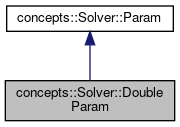
\includegraphics[width=207pt]{classconcepts_1_1_solver_1_1_double_param__inherit__graph}
\end{center}
\end{figure}


Collaboration diagram for concepts\+:\+:Solver\+:\+:Double\+Param\+:\nopagebreak
\begin{figure}[H]
\begin{center}
\leavevmode
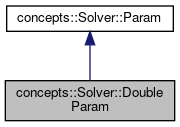
\includegraphics[width=207pt]{classconcepts_1_1_solver_1_1_double_param__coll__graph}
\end{center}
\end{figure}
\subsection*{Public Member Functions}
\begin{DoxyCompactItemize}
\item 
\hyperlink{classconcepts_1_1_solver_1_1_double_param_a4f432bf3bd5872439e9d04245f016608}{Double\+Param} (double v)
\item 
void \hyperlink{classconcepts_1_1_solver_1_1_double_param_a9d9cf1f190f8e7b7c4840f0d44fefa1b}{parse} (const char $\ast$arg)
\item 
void \hyperlink{classconcepts_1_1_solver_1_1_double_param_a006e726301f821c96edb00b4ca2ea345}{set} (bool v)
\item 
void \hyperlink{classconcepts_1_1_solver_1_1_double_param_a4648d672a792ded79977319d968fd497}{set} (int v)
\item 
void \hyperlink{classconcepts_1_1_solver_1_1_double_param_a5a27e7e058121b520d71472e8de549db}{set} (double v)
\item 
bool \hyperlink{classconcepts_1_1_solver_1_1_double_param_a59c7fa9b821c071f13d6182d6b525473}{get\+Bool} () const
\item 
int \hyperlink{classconcepts_1_1_solver_1_1_double_param_a19c83a217a6b73891548850869e9c230}{get\+Int} () const
\item 
double \hyperlink{classconcepts_1_1_solver_1_1_double_param_a39d5bb1d5b33ef84c8c015b977b438d9}{get\+Double} () const
\item 
std\+::string \hyperlink{classconcepts_1_1_solver_1_1_double_param_a536f65af0681a1e3af0e101f952f717c}{to\+String} () const
\end{DoxyCompactItemize}
\subsection*{Protected Attributes}
\begin{DoxyCompactItemize}
\item 
double \hyperlink{classconcepts_1_1_solver_1_1_double_param_af41548e144e9d6e09188c969740d3507}{value}
\end{DoxyCompactItemize}


\subsection{Constructor \& Destructor Documentation}
\mbox{\Hypertarget{classconcepts_1_1_solver_1_1_double_param_a4f432bf3bd5872439e9d04245f016608}\label{classconcepts_1_1_solver_1_1_double_param_a4f432bf3bd5872439e9d04245f016608}} 
\index{concepts\+::\+Solver\+::\+Double\+Param@{concepts\+::\+Solver\+::\+Double\+Param}!Double\+Param@{Double\+Param}}
\index{Double\+Param@{Double\+Param}!concepts\+::\+Solver\+::\+Double\+Param@{concepts\+::\+Solver\+::\+Double\+Param}}
\subsubsection{\texorpdfstring{Double\+Param()}{DoubleParam()}}
{\footnotesize\ttfamily concepts\+::\+Solver\+::\+Double\+Param\+::\+Double\+Param (\begin{DoxyParamCaption}\item[{double}]{v }\end{DoxyParamCaption})\hspace{0.3cm}{\ttfamily [inline]}}



\subsection{Member Function Documentation}
\mbox{\Hypertarget{classconcepts_1_1_solver_1_1_double_param_a59c7fa9b821c071f13d6182d6b525473}\label{classconcepts_1_1_solver_1_1_double_param_a59c7fa9b821c071f13d6182d6b525473}} 
\index{concepts\+::\+Solver\+::\+Double\+Param@{concepts\+::\+Solver\+::\+Double\+Param}!get\+Bool@{get\+Bool}}
\index{get\+Bool@{get\+Bool}!concepts\+::\+Solver\+::\+Double\+Param@{concepts\+::\+Solver\+::\+Double\+Param}}
\subsubsection{\texorpdfstring{get\+Bool()}{getBool()}}
{\footnotesize\ttfamily bool concepts\+::\+Solver\+::\+Double\+Param\+::get\+Bool (\begin{DoxyParamCaption}{ }\end{DoxyParamCaption}) const\hspace{0.3cm}{\ttfamily [inline]}, {\ttfamily [virtual]}}



Implements \hyperlink{classconcepts_1_1_solver_1_1_param_aaca8a78f4669d189764e9e654143d705}{concepts\+::\+Solver\+::\+Param}.

\mbox{\Hypertarget{classconcepts_1_1_solver_1_1_double_param_a39d5bb1d5b33ef84c8c015b977b438d9}\label{classconcepts_1_1_solver_1_1_double_param_a39d5bb1d5b33ef84c8c015b977b438d9}} 
\index{concepts\+::\+Solver\+::\+Double\+Param@{concepts\+::\+Solver\+::\+Double\+Param}!get\+Double@{get\+Double}}
\index{get\+Double@{get\+Double}!concepts\+::\+Solver\+::\+Double\+Param@{concepts\+::\+Solver\+::\+Double\+Param}}
\subsubsection{\texorpdfstring{get\+Double()}{getDouble()}}
{\footnotesize\ttfamily double concepts\+::\+Solver\+::\+Double\+Param\+::get\+Double (\begin{DoxyParamCaption}{ }\end{DoxyParamCaption}) const\hspace{0.3cm}{\ttfamily [inline]}, {\ttfamily [virtual]}}



Implements \hyperlink{classconcepts_1_1_solver_1_1_param_a50d288b81da0b77d342e46e75f9b4bfc}{concepts\+::\+Solver\+::\+Param}.

\mbox{\Hypertarget{classconcepts_1_1_solver_1_1_double_param_a19c83a217a6b73891548850869e9c230}\label{classconcepts_1_1_solver_1_1_double_param_a19c83a217a6b73891548850869e9c230}} 
\index{concepts\+::\+Solver\+::\+Double\+Param@{concepts\+::\+Solver\+::\+Double\+Param}!get\+Int@{get\+Int}}
\index{get\+Int@{get\+Int}!concepts\+::\+Solver\+::\+Double\+Param@{concepts\+::\+Solver\+::\+Double\+Param}}
\subsubsection{\texorpdfstring{get\+Int()}{getInt()}}
{\footnotesize\ttfamily int concepts\+::\+Solver\+::\+Double\+Param\+::get\+Int (\begin{DoxyParamCaption}{ }\end{DoxyParamCaption}) const\hspace{0.3cm}{\ttfamily [inline]}, {\ttfamily [virtual]}}



Implements \hyperlink{classconcepts_1_1_solver_1_1_param_ab849633a029055c00d828df3adb0546e}{concepts\+::\+Solver\+::\+Param}.

\mbox{\Hypertarget{classconcepts_1_1_solver_1_1_double_param_a9d9cf1f190f8e7b7c4840f0d44fefa1b}\label{classconcepts_1_1_solver_1_1_double_param_a9d9cf1f190f8e7b7c4840f0d44fefa1b}} 
\index{concepts\+::\+Solver\+::\+Double\+Param@{concepts\+::\+Solver\+::\+Double\+Param}!parse@{parse}}
\index{parse@{parse}!concepts\+::\+Solver\+::\+Double\+Param@{concepts\+::\+Solver\+::\+Double\+Param}}
\subsubsection{\texorpdfstring{parse()}{parse()}}
{\footnotesize\ttfamily void concepts\+::\+Solver\+::\+Double\+Param\+::parse (\begin{DoxyParamCaption}\item[{const char $\ast$}]{arg }\end{DoxyParamCaption})\hspace{0.3cm}{\ttfamily [inline]}, {\ttfamily [virtual]}}



Implements \hyperlink{classconcepts_1_1_solver_1_1_param_a0c2e4d895747668b01339db9226eceae}{concepts\+::\+Solver\+::\+Param}.

\mbox{\Hypertarget{classconcepts_1_1_solver_1_1_double_param_a006e726301f821c96edb00b4ca2ea345}\label{classconcepts_1_1_solver_1_1_double_param_a006e726301f821c96edb00b4ca2ea345}} 
\index{concepts\+::\+Solver\+::\+Double\+Param@{concepts\+::\+Solver\+::\+Double\+Param}!set@{set}}
\index{set@{set}!concepts\+::\+Solver\+::\+Double\+Param@{concepts\+::\+Solver\+::\+Double\+Param}}
\subsubsection{\texorpdfstring{set()}{set()}\hspace{0.1cm}{\footnotesize\ttfamily [1/3]}}
{\footnotesize\ttfamily void concepts\+::\+Solver\+::\+Double\+Param\+::set (\begin{DoxyParamCaption}\item[{bool}]{v }\end{DoxyParamCaption})\hspace{0.3cm}{\ttfamily [inline]}, {\ttfamily [virtual]}}



Implements \hyperlink{classconcepts_1_1_solver_1_1_param_aa525a1a88dd771eaf5d66f35323fbb86}{concepts\+::\+Solver\+::\+Param}.

\mbox{\Hypertarget{classconcepts_1_1_solver_1_1_double_param_a4648d672a792ded79977319d968fd497}\label{classconcepts_1_1_solver_1_1_double_param_a4648d672a792ded79977319d968fd497}} 
\index{concepts\+::\+Solver\+::\+Double\+Param@{concepts\+::\+Solver\+::\+Double\+Param}!set@{set}}
\index{set@{set}!concepts\+::\+Solver\+::\+Double\+Param@{concepts\+::\+Solver\+::\+Double\+Param}}
\subsubsection{\texorpdfstring{set()}{set()}\hspace{0.1cm}{\footnotesize\ttfamily [2/3]}}
{\footnotesize\ttfamily void concepts\+::\+Solver\+::\+Double\+Param\+::set (\begin{DoxyParamCaption}\item[{int}]{v }\end{DoxyParamCaption})\hspace{0.3cm}{\ttfamily [inline]}, {\ttfamily [virtual]}}



Implements \hyperlink{classconcepts_1_1_solver_1_1_param_ad3de8144a70e67eeae4278f534e46274}{concepts\+::\+Solver\+::\+Param}.

\mbox{\Hypertarget{classconcepts_1_1_solver_1_1_double_param_a5a27e7e058121b520d71472e8de549db}\label{classconcepts_1_1_solver_1_1_double_param_a5a27e7e058121b520d71472e8de549db}} 
\index{concepts\+::\+Solver\+::\+Double\+Param@{concepts\+::\+Solver\+::\+Double\+Param}!set@{set}}
\index{set@{set}!concepts\+::\+Solver\+::\+Double\+Param@{concepts\+::\+Solver\+::\+Double\+Param}}
\subsubsection{\texorpdfstring{set()}{set()}\hspace{0.1cm}{\footnotesize\ttfamily [3/3]}}
{\footnotesize\ttfamily void concepts\+::\+Solver\+::\+Double\+Param\+::set (\begin{DoxyParamCaption}\item[{double}]{v }\end{DoxyParamCaption})\hspace{0.3cm}{\ttfamily [inline]}, {\ttfamily [virtual]}}



Implements \hyperlink{classconcepts_1_1_solver_1_1_param_a35b7155d8f6db1b3e63e60b883beebcb}{concepts\+::\+Solver\+::\+Param}.

\mbox{\Hypertarget{classconcepts_1_1_solver_1_1_double_param_a536f65af0681a1e3af0e101f952f717c}\label{classconcepts_1_1_solver_1_1_double_param_a536f65af0681a1e3af0e101f952f717c}} 
\index{concepts\+::\+Solver\+::\+Double\+Param@{concepts\+::\+Solver\+::\+Double\+Param}!to\+String@{to\+String}}
\index{to\+String@{to\+String}!concepts\+::\+Solver\+::\+Double\+Param@{concepts\+::\+Solver\+::\+Double\+Param}}
\subsubsection{\texorpdfstring{to\+String()}{toString()}}
{\footnotesize\ttfamily std\+::string concepts\+::\+Solver\+::\+Double\+Param\+::to\+String (\begin{DoxyParamCaption}{ }\end{DoxyParamCaption}) const\hspace{0.3cm}{\ttfamily [inline]}, {\ttfamily [virtual]}}



Implements \hyperlink{classconcepts_1_1_solver_1_1_param_abcbd9c68852499c7be9ebf6a2d22f4b5}{concepts\+::\+Solver\+::\+Param}.



\subsection{Member Data Documentation}
\mbox{\Hypertarget{classconcepts_1_1_solver_1_1_double_param_af41548e144e9d6e09188c969740d3507}\label{classconcepts_1_1_solver_1_1_double_param_af41548e144e9d6e09188c969740d3507}} 
\index{concepts\+::\+Solver\+::\+Double\+Param@{concepts\+::\+Solver\+::\+Double\+Param}!value@{value}}
\index{value@{value}!concepts\+::\+Solver\+::\+Double\+Param@{concepts\+::\+Solver\+::\+Double\+Param}}
\subsubsection{\texorpdfstring{value}{value}}
{\footnotesize\ttfamily double concepts\+::\+Solver\+::\+Double\+Param\+::value\hspace{0.3cm}{\ttfamily [protected]}}



The documentation for this class was generated from the following file\+:\begin{DoxyCompactItemize}
\item 
/home/plaiseek/\+Projects/landscape\+\_\+opt\+\_\+cpp/include/solvers/concept/\hyperlink{solver_8hpp}{solver.\+hpp}\end{DoxyCompactItemize}

\hypertarget{class_e_c_a}{}\section{E\+CA Class Reference}
\label{class_e_c_a}\index{E\+CA@{E\+CA}}


{\ttfamily \#include $<$eca.\+hpp$>$}



Inheritance diagram for E\+CA\+:\nopagebreak
\begin{figure}[H]
\begin{center}
\leavevmode
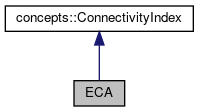
\includegraphics[width=221pt]{class_e_c_a__inherit__graph}
\end{center}
\end{figure}


Collaboration diagram for E\+CA\+:\nopagebreak
\begin{figure}[H]
\begin{center}
\leavevmode
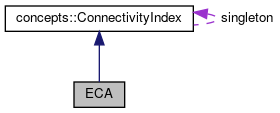
\includegraphics[width=282pt]{class_e_c_a__coll__graph}
\end{center}
\end{figure}
\subsection*{Public Member Functions}
\begin{DoxyCompactItemize}
\item 
\hyperlink{class_e_c_a_acc7762273f9df84a3457c8c9b4e58a31}{$\sim$\+E\+CA} ()
\item 
double \hyperlink{class_e_c_a_ae4d2665232d2ff83b3f04f812c45c172}{eval\+\_\+solution} (const \hyperlink{class_landscape}{Landscape} \&landscape, const \hyperlink{class_solution}{Solution} \&solution) const
\item 
{\footnotesize template$<$typename GR , typename QM , typename PM , typename CM $>$ }\\double \hyperlink{class_e_c_a_af8127c6291b457b8c7033f23d1656767}{eval} (const \hyperlink{classconcepts_1_1_abstract_landscape}{concepts\+::\+Abstract\+Landscape}$<$ GR, QM, PM, CM $>$ \&landscape, const typename G\+R\+::template Node\+Map$<$ bool $>$ \&node\+Filter)
\begin{DoxyCompactList}\small\item\em Computes the value of the \hyperlink{class_e_c_a}{E\+CA} index of the specified landscape. \end{DoxyCompactList}\item 
{\footnotesize template$<$typename GR , typename QM , typename PM , typename CM $>$ }\\double \hyperlink{class_e_c_a_ab6556319590259a816cf176e933746d7}{eval} (const \hyperlink{classconcepts_1_1_abstract_landscape}{concepts\+::\+Abstract\+Landscape}$<$ GR, QM, PM, CM $>$ \&landscape)
\begin{DoxyCompactList}\small\item\em Computes the value of the \hyperlink{class_e_c_a}{E\+CA} index of the specified landscape. \end{DoxyCompactList}\end{DoxyCompactItemize}
\subsection*{Static Public Member Functions}
\begin{DoxyCompactItemize}
\item 
static \hyperlink{class_e_c_a}{E\+CA} \& \hyperlink{class_e_c_a_ac7d3fd1b819ca2200c0eb6817d464323}{get} () noexcept
\item 
static double \hyperlink{class_e_c_a_ad9a7a487c43cecdaea971ffba0098474}{P\+\_\+func} (const double d, const double alpha)
\item 
static double \hyperlink{class_e_c_a_ae39dbd10fc9c65479cbf6b7b09339590}{inv\+\_\+\+P\+\_\+func} (const double p, const double alpha)
\end{DoxyCompactItemize}
\subsection*{Additional Inherited Members}


\subsection{Constructor \& Destructor Documentation}
\mbox{\Hypertarget{class_e_c_a_acc7762273f9df84a3457c8c9b4e58a31}\label{class_e_c_a_acc7762273f9df84a3457c8c9b4e58a31}} 
\index{E\+CA@{E\+CA}!````~E\+CA@{$\sim$\+E\+CA}}
\index{````~E\+CA@{$\sim$\+E\+CA}!E\+CA@{E\+CA}}
\subsubsection{\texorpdfstring{$\sim$\+E\+C\+A()}{~ECA()}}
{\footnotesize\ttfamily E\+C\+A\+::$\sim$\+E\+CA (\begin{DoxyParamCaption}{ }\end{DoxyParamCaption})}



\subsection{Member Function Documentation}
\mbox{\Hypertarget{class_e_c_a_af8127c6291b457b8c7033f23d1656767}\label{class_e_c_a_af8127c6291b457b8c7033f23d1656767}} 
\index{E\+CA@{E\+CA}!eval@{eval}}
\index{eval@{eval}!E\+CA@{E\+CA}}
\subsubsection{\texorpdfstring{eval()}{eval()}\hspace{0.1cm}{\footnotesize\ttfamily [1/2]}}
{\footnotesize\ttfamily template$<$typename GR , typename QM , typename PM , typename CM $>$ \\
double E\+C\+A\+::eval (\begin{DoxyParamCaption}\item[{const \hyperlink{classconcepts_1_1_abstract_landscape}{concepts\+::\+Abstract\+Landscape}$<$ GR, QM, PM, CM $>$ \&}]{landscape,  }\item[{const typename G\+R\+::template Node\+Map$<$ bool $>$ \&}]{node\+Filter }\end{DoxyParamCaption})\hspace{0.3cm}{\ttfamily [inline]}}



Computes the value of the \hyperlink{class_e_c_a}{E\+CA} index of the specified landscape. 

\begin{DoxyRefDesc}{Time Complexity}
\item[\hyperlink{time__time000005}{Time Complexity}]$O(n \cdot (m + n) \log n)$ where $n$ is the number of nodes and $m$ the number of arcs \end{DoxyRefDesc}
\begin{DoxyRefDesc}{Space Complexity}
\item[\hyperlink{space__space000005}{Space Complexity}]$O(m)$ where $m$ is the number of arcs \end{DoxyRefDesc}
\mbox{\Hypertarget{class_e_c_a_ab6556319590259a816cf176e933746d7}\label{class_e_c_a_ab6556319590259a816cf176e933746d7}} 
\index{E\+CA@{E\+CA}!eval@{eval}}
\index{eval@{eval}!E\+CA@{E\+CA}}
\subsubsection{\texorpdfstring{eval()}{eval()}\hspace{0.1cm}{\footnotesize\ttfamily [2/2]}}
{\footnotesize\ttfamily template$<$typename GR , typename QM , typename PM , typename CM $>$ \\
double E\+C\+A\+::eval (\begin{DoxyParamCaption}\item[{const \hyperlink{classconcepts_1_1_abstract_landscape}{concepts\+::\+Abstract\+Landscape}$<$ GR, QM, PM, CM $>$ \&}]{landscape }\end{DoxyParamCaption})\hspace{0.3cm}{\ttfamily [inline]}}



Computes the value of the \hyperlink{class_e_c_a}{E\+CA} index of the specified landscape. 

\begin{DoxyRefDesc}{Time Complexity}
\item[\hyperlink{time__time000006}{Time Complexity}]$O(n \cdot (m + n) \log n)$ where $n$ is the number of nodes and $m$ the number of arcs \end{DoxyRefDesc}
\begin{DoxyRefDesc}{Space Complexity}
\item[\hyperlink{space__space000006}{Space Complexity}]$O(m)$ running and $O(1)$ returning where $m$ is the number of arcs \end{DoxyRefDesc}
\mbox{\Hypertarget{class_e_c_a_ae4d2665232d2ff83b3f04f812c45c172}\label{class_e_c_a_ae4d2665232d2ff83b3f04f812c45c172}} 
\index{E\+CA@{E\+CA}!eval\+\_\+solution@{eval\+\_\+solution}}
\index{eval\+\_\+solution@{eval\+\_\+solution}!E\+CA@{E\+CA}}
\subsubsection{\texorpdfstring{eval\+\_\+solution()}{eval\_solution()}}
{\footnotesize\ttfamily double E\+C\+A\+::eval\+\_\+solution (\begin{DoxyParamCaption}\item[{const \hyperlink{class_landscape}{Landscape} \&}]{landscape,  }\item[{const \hyperlink{class_solution}{Solution} \&}]{solution }\end{DoxyParamCaption}) const}

\mbox{\Hypertarget{class_e_c_a_ac7d3fd1b819ca2200c0eb6817d464323}\label{class_e_c_a_ac7d3fd1b819ca2200c0eb6817d464323}} 
\index{E\+CA@{E\+CA}!get@{get}}
\index{get@{get}!E\+CA@{E\+CA}}
\subsubsection{\texorpdfstring{get()}{get()}}
{\footnotesize\ttfamily static \hyperlink{class_e_c_a}{E\+CA}\& E\+C\+A\+::get (\begin{DoxyParamCaption}{ }\end{DoxyParamCaption})\hspace{0.3cm}{\ttfamily [inline]}, {\ttfamily [static]}, {\ttfamily [noexcept]}}

\mbox{\Hypertarget{class_e_c_a_ae39dbd10fc9c65479cbf6b7b09339590}\label{class_e_c_a_ae39dbd10fc9c65479cbf6b7b09339590}} 
\index{E\+CA@{E\+CA}!inv\+\_\+\+P\+\_\+func@{inv\+\_\+\+P\+\_\+func}}
\index{inv\+\_\+\+P\+\_\+func@{inv\+\_\+\+P\+\_\+func}!E\+CA@{E\+CA}}
\subsubsection{\texorpdfstring{inv\+\_\+\+P\+\_\+func()}{inv\_P\_func()}}
{\footnotesize\ttfamily static double E\+C\+A\+::inv\+\_\+\+P\+\_\+func (\begin{DoxyParamCaption}\item[{const double}]{p,  }\item[{const double}]{alpha }\end{DoxyParamCaption})\hspace{0.3cm}{\ttfamily [inline]}, {\ttfamily [static]}}

\mbox{\Hypertarget{class_e_c_a_ad9a7a487c43cecdaea971ffba0098474}\label{class_e_c_a_ad9a7a487c43cecdaea971ffba0098474}} 
\index{E\+CA@{E\+CA}!P\+\_\+func@{P\+\_\+func}}
\index{P\+\_\+func@{P\+\_\+func}!E\+CA@{E\+CA}}
\subsubsection{\texorpdfstring{P\+\_\+func()}{P\_func()}}
{\footnotesize\ttfamily static double E\+C\+A\+::\+P\+\_\+func (\begin{DoxyParamCaption}\item[{const double}]{d,  }\item[{const double}]{alpha }\end{DoxyParamCaption})\hspace{0.3cm}{\ttfamily [inline]}, {\ttfamily [static]}}



The documentation for this class was generated from the following files\+:\begin{DoxyCompactItemize}
\item 
/home/plaiseek/\+Projects/landscape\+\_\+opt\+\_\+cpp/include/indices/\hyperlink{eca_8hpp}{eca.\+hpp}\item 
/home/plaiseek/\+Projects/landscape\+\_\+opt\+\_\+cpp/src/indices/\hyperlink{eca_8cpp}{eca.\+cpp}\end{DoxyCompactItemize}

\hypertarget{class_e_c_a_reff}{}\section{E\+C\+A\+Reff Class Reference}
\label{class_e_c_a_reff}\index{E\+C\+A\+Reff@{E\+C\+A\+Reff}}


{\ttfamily \#include $<$ecareff.\+hpp$>$}



Inheritance diagram for E\+C\+A\+Reff\+:\nopagebreak
\begin{figure}[H]
\begin{center}
\leavevmode
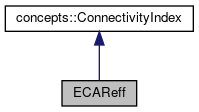
\includegraphics[width=221pt]{class_e_c_a_reff__inherit__graph}
\end{center}
\end{figure}


Collaboration diagram for E\+C\+A\+Reff\+:\nopagebreak
\begin{figure}[H]
\begin{center}
\leavevmode
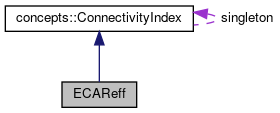
\includegraphics[width=282pt]{class_e_c_a_reff__coll__graph}
\end{center}
\end{figure}
\subsection*{Public Member Functions}
\begin{DoxyCompactItemize}
\item 
\hyperlink{class_e_c_a_reff_ae1a03ebc18f59b302e11cc3f88570562}{$\sim$\+E\+C\+A\+Reff} ()
\item 
{\footnotesize template$<$typename GR , typename DM $>$ }\\G\+R\+::template Node\+Map$<$ typename G\+R\+::template Node\+Map$<$ double $>$ $\ast$ $>$ $\ast$ \hyperlink{class_e_c_a_reff_afa9b4d597a1771f154eb1179ebfcfd7c}{get\+Reff} (const GR \&g, const DM \&resistance)
\item 
{\footnotesize template$<$typename GR , typename QM , typename DM , typename CM $>$ }\\double \hyperlink{class_e_c_a_reff_a6ae1382bfd570347211838b7fa34b7c7}{eval} (const \hyperlink{classconcepts_1_1_abstract_landscape}{concepts\+::\+Abstract\+Landscape}$<$ GR, QM, DM, CM $>$ \&landscape)
\end{DoxyCompactItemize}
\subsection*{Static Public Member Functions}
\begin{DoxyCompactItemize}
\item 
static \hyperlink{class_e_c_a_reff}{E\+C\+A\+Reff} \& \hyperlink{class_e_c_a_reff_af6d8a1284a194d55123e8a878127c45d}{get} () noexcept
\end{DoxyCompactItemize}
\subsection*{Additional Inherited Members}


\subsection{Constructor \& Destructor Documentation}
\mbox{\Hypertarget{class_e_c_a_reff_ae1a03ebc18f59b302e11cc3f88570562}\label{class_e_c_a_reff_ae1a03ebc18f59b302e11cc3f88570562}} 
\index{E\+C\+A\+Reff@{E\+C\+A\+Reff}!````~E\+C\+A\+Reff@{$\sim$\+E\+C\+A\+Reff}}
\index{````~E\+C\+A\+Reff@{$\sim$\+E\+C\+A\+Reff}!E\+C\+A\+Reff@{E\+C\+A\+Reff}}
\subsubsection{\texorpdfstring{$\sim$\+E\+C\+A\+Reff()}{~ECAReff()}}
{\footnotesize\ttfamily E\+C\+A\+Reff\+::$\sim$\+E\+C\+A\+Reff (\begin{DoxyParamCaption}{ }\end{DoxyParamCaption})}



\subsection{Member Function Documentation}
\mbox{\Hypertarget{class_e_c_a_reff_a6ae1382bfd570347211838b7fa34b7c7}\label{class_e_c_a_reff_a6ae1382bfd570347211838b7fa34b7c7}} 
\index{E\+C\+A\+Reff@{E\+C\+A\+Reff}!eval@{eval}}
\index{eval@{eval}!E\+C\+A\+Reff@{E\+C\+A\+Reff}}
\subsubsection{\texorpdfstring{eval()}{eval()}}
{\footnotesize\ttfamily template$<$typename GR , typename QM , typename DM , typename CM $>$ \\
double E\+C\+A\+Reff\+::eval (\begin{DoxyParamCaption}\item[{const \hyperlink{classconcepts_1_1_abstract_landscape}{concepts\+::\+Abstract\+Landscape}$<$ GR, QM, DM, CM $>$ \&}]{landscape }\end{DoxyParamCaption})}

\mbox{\Hypertarget{class_e_c_a_reff_af6d8a1284a194d55123e8a878127c45d}\label{class_e_c_a_reff_af6d8a1284a194d55123e8a878127c45d}} 
\index{E\+C\+A\+Reff@{E\+C\+A\+Reff}!get@{get}}
\index{get@{get}!E\+C\+A\+Reff@{E\+C\+A\+Reff}}
\subsubsection{\texorpdfstring{get()}{get()}}
{\footnotesize\ttfamily static \hyperlink{class_e_c_a_reff}{E\+C\+A\+Reff}\& E\+C\+A\+Reff\+::get (\begin{DoxyParamCaption}{ }\end{DoxyParamCaption})\hspace{0.3cm}{\ttfamily [inline]}, {\ttfamily [static]}, {\ttfamily [noexcept]}}

\mbox{\Hypertarget{class_e_c_a_reff_afa9b4d597a1771f154eb1179ebfcfd7c}\label{class_e_c_a_reff_afa9b4d597a1771f154eb1179ebfcfd7c}} 
\index{E\+C\+A\+Reff@{E\+C\+A\+Reff}!get\+Reff@{get\+Reff}}
\index{get\+Reff@{get\+Reff}!E\+C\+A\+Reff@{E\+C\+A\+Reff}}
\subsubsection{\texorpdfstring{get\+Reff()}{getReff()}}
{\footnotesize\ttfamily template$<$typename GR , typename DM $>$ \\
G\+R\+::template Node\+Map$<$ typename G\+R\+::template Node\+Map$<$ double $>$ $\ast$ $>$ $\ast$ E\+C\+A\+Reff\+::get\+Reff (\begin{DoxyParamCaption}\item[{const GR \&}]{g,  }\item[{const DM \&}]{resistance }\end{DoxyParamCaption})}



The documentation for this class was generated from the following files\+:\begin{DoxyCompactItemize}
\item 
/home/plaiseek/\+Projects/landscape\+\_\+opt\+\_\+cpp/include/indices/\hyperlink{ecareff_8hpp}{ecareff.\+hpp}\item 
/home/plaiseek/\+Projects/landscape\+\_\+opt\+\_\+cpp/src/indices/\hyperlink{ecareff_8cpp}{ecareff.\+cpp}\end{DoxyCompactItemize}

\hypertarget{class_solvers_1_1_p_l___e_c_a__2___vars_1_1_f_var}{}\section{Solvers\+:\+:P\+L\+\_\+\+E\+C\+A\+\_\+2\+\_\+\+Vars\+:\+:F\+Var Class Reference}
\label{class_solvers_1_1_p_l___e_c_a__2___vars_1_1_f_var}\index{Solvers\+::\+P\+L\+\_\+\+E\+C\+A\+\_\+2\+\_\+\+Vars\+::\+F\+Var@{Solvers\+::\+P\+L\+\_\+\+E\+C\+A\+\_\+2\+\_\+\+Vars\+::\+F\+Var}}


Inheritance diagram for Solvers\+:\+:P\+L\+\_\+\+E\+C\+A\+\_\+2\+\_\+\+Vars\+:\+:F\+Var\+:\nopagebreak
\begin{figure}[H]
\begin{center}
\leavevmode
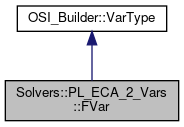
\includegraphics[width=210pt]{class_solvers_1_1_p_l___e_c_a__2___vars_1_1_f_var__inherit__graph}
\end{center}
\end{figure}


Collaboration diagram for Solvers\+:\+:P\+L\+\_\+\+E\+C\+A\+\_\+2\+\_\+\+Vars\+:\+:F\+Var\+:\nopagebreak
\begin{figure}[H]
\begin{center}
\leavevmode
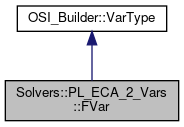
\includegraphics[width=210pt]{class_solvers_1_1_p_l___e_c_a__2___vars_1_1_f_var__coll__graph}
\end{center}
\end{figure}
\subsection*{Public Member Functions}
\begin{DoxyCompactItemize}
\item 
\hyperlink{class_solvers_1_1_p_l___e_c_a__2___vars_1_1_f_var_a7ee1990a04e40785a54626cc41417573}{F\+Var} (const \hyperlink{pl__reff_8cpp_a65aea14f39d53b24df9910d54216d620}{Graph\+\_\+t} \&graph, int n)
\item 
int \hyperlink{class_solvers_1_1_p_l___e_c_a__2___vars_1_1_f_var_a3e092894e61d1d3a09431d021a3d2cde}{id} (Graph\+\_\+t\+::\+Node u)
\end{DoxyCompactItemize}
\subsection*{Additional Inherited Members}


\subsection{Constructor \& Destructor Documentation}
\mbox{\Hypertarget{class_solvers_1_1_p_l___e_c_a__2___vars_1_1_f_var_a7ee1990a04e40785a54626cc41417573}\label{class_solvers_1_1_p_l___e_c_a__2___vars_1_1_f_var_a7ee1990a04e40785a54626cc41417573}} 
\index{Solvers\+::\+P\+L\+\_\+\+E\+C\+A\+\_\+2\+\_\+\+Vars\+::\+F\+Var@{Solvers\+::\+P\+L\+\_\+\+E\+C\+A\+\_\+2\+\_\+\+Vars\+::\+F\+Var}!F\+Var@{F\+Var}}
\index{F\+Var@{F\+Var}!Solvers\+::\+P\+L\+\_\+\+E\+C\+A\+\_\+2\+\_\+\+Vars\+::\+F\+Var@{Solvers\+::\+P\+L\+\_\+\+E\+C\+A\+\_\+2\+\_\+\+Vars\+::\+F\+Var}}
\subsubsection{\texorpdfstring{F\+Var()}{FVar()}}
{\footnotesize\ttfamily Solvers\+::\+P\+L\+\_\+\+E\+C\+A\+\_\+2\+\_\+\+Vars\+::\+F\+Var\+::\+F\+Var (\begin{DoxyParamCaption}\item[{const \hyperlink{pl__reff_8cpp_a65aea14f39d53b24df9910d54216d620}{Graph\+\_\+t} \&}]{graph,  }\item[{int}]{n }\end{DoxyParamCaption})\hspace{0.3cm}{\ttfamily [inline]}}



\subsection{Member Function Documentation}
\mbox{\Hypertarget{class_solvers_1_1_p_l___e_c_a__2___vars_1_1_f_var_a3e092894e61d1d3a09431d021a3d2cde}\label{class_solvers_1_1_p_l___e_c_a__2___vars_1_1_f_var_a3e092894e61d1d3a09431d021a3d2cde}} 
\index{Solvers\+::\+P\+L\+\_\+\+E\+C\+A\+\_\+2\+\_\+\+Vars\+::\+F\+Var@{Solvers\+::\+P\+L\+\_\+\+E\+C\+A\+\_\+2\+\_\+\+Vars\+::\+F\+Var}!id@{id}}
\index{id@{id}!Solvers\+::\+P\+L\+\_\+\+E\+C\+A\+\_\+2\+\_\+\+Vars\+::\+F\+Var@{Solvers\+::\+P\+L\+\_\+\+E\+C\+A\+\_\+2\+\_\+\+Vars\+::\+F\+Var}}
\subsubsection{\texorpdfstring{id()}{id()}}
{\footnotesize\ttfamily int Solvers\+::\+P\+L\+\_\+\+E\+C\+A\+\_\+2\+\_\+\+Vars\+::\+F\+Var\+::id (\begin{DoxyParamCaption}\item[{Graph\+\_\+t\+::\+Node}]{u }\end{DoxyParamCaption})\hspace{0.3cm}{\ttfamily [inline]}}



The documentation for this class was generated from the following file\+:\begin{DoxyCompactItemize}
\item 
/home/plaiseek/\+Projects/landscape\+\_\+opt\+\_\+cpp/src/solvers/\hyperlink{pl__eca__2_8cpp}{pl\+\_\+eca\+\_\+2.\+cpp}\end{DoxyCompactItemize}

\hypertarget{class_solvers_1_1_p_l___e_c_a__3___vars_1_1_f_var}{}\section{Solvers\+:\+:P\+L\+\_\+\+E\+C\+A\+\_\+3\+\_\+\+Vars\+:\+:F\+Var Class Reference}
\label{class_solvers_1_1_p_l___e_c_a__3___vars_1_1_f_var}\index{Solvers\+::\+P\+L\+\_\+\+E\+C\+A\+\_\+3\+\_\+\+Vars\+::\+F\+Var@{Solvers\+::\+P\+L\+\_\+\+E\+C\+A\+\_\+3\+\_\+\+Vars\+::\+F\+Var}}


Inheritance diagram for Solvers\+:\+:P\+L\+\_\+\+E\+C\+A\+\_\+3\+\_\+\+Vars\+:\+:F\+Var\+:\nopagebreak
\begin{figure}[H]
\begin{center}
\leavevmode
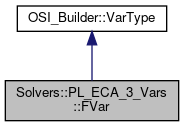
\includegraphics[width=210pt]{class_solvers_1_1_p_l___e_c_a__3___vars_1_1_f_var__inherit__graph}
\end{center}
\end{figure}


Collaboration diagram for Solvers\+:\+:P\+L\+\_\+\+E\+C\+A\+\_\+3\+\_\+\+Vars\+:\+:F\+Var\+:\nopagebreak
\begin{figure}[H]
\begin{center}
\leavevmode
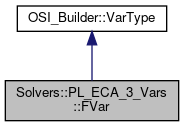
\includegraphics[width=210pt]{class_solvers_1_1_p_l___e_c_a__3___vars_1_1_f_var__coll__graph}
\end{center}
\end{figure}
\subsection*{Public Member Functions}
\begin{DoxyCompactItemize}
\item 
\hyperlink{class_solvers_1_1_p_l___e_c_a__3___vars_1_1_f_var_af913d0630b68754b3f19e84ec022fa6e}{F\+Var} ()
\item 
int \hyperlink{class_solvers_1_1_p_l___e_c_a__3___vars_1_1_f_var_a4f84286d12212ae32eb4c8fde3f8916f}{id} () const
\end{DoxyCompactItemize}
\subsection*{Additional Inherited Members}


\subsection{Constructor \& Destructor Documentation}
\mbox{\Hypertarget{class_solvers_1_1_p_l___e_c_a__3___vars_1_1_f_var_af913d0630b68754b3f19e84ec022fa6e}\label{class_solvers_1_1_p_l___e_c_a__3___vars_1_1_f_var_af913d0630b68754b3f19e84ec022fa6e}} 
\index{Solvers\+::\+P\+L\+\_\+\+E\+C\+A\+\_\+3\+\_\+\+Vars\+::\+F\+Var@{Solvers\+::\+P\+L\+\_\+\+E\+C\+A\+\_\+3\+\_\+\+Vars\+::\+F\+Var}!F\+Var@{F\+Var}}
\index{F\+Var@{F\+Var}!Solvers\+::\+P\+L\+\_\+\+E\+C\+A\+\_\+3\+\_\+\+Vars\+::\+F\+Var@{Solvers\+::\+P\+L\+\_\+\+E\+C\+A\+\_\+3\+\_\+\+Vars\+::\+F\+Var}}
\subsubsection{\texorpdfstring{F\+Var()}{FVar()}}
{\footnotesize\ttfamily Solvers\+::\+P\+L\+\_\+\+E\+C\+A\+\_\+3\+\_\+\+Vars\+::\+F\+Var\+::\+F\+Var (\begin{DoxyParamCaption}{ }\end{DoxyParamCaption})\hspace{0.3cm}{\ttfamily [inline]}}



\subsection{Member Function Documentation}
\mbox{\Hypertarget{class_solvers_1_1_p_l___e_c_a__3___vars_1_1_f_var_a4f84286d12212ae32eb4c8fde3f8916f}\label{class_solvers_1_1_p_l___e_c_a__3___vars_1_1_f_var_a4f84286d12212ae32eb4c8fde3f8916f}} 
\index{Solvers\+::\+P\+L\+\_\+\+E\+C\+A\+\_\+3\+\_\+\+Vars\+::\+F\+Var@{Solvers\+::\+P\+L\+\_\+\+E\+C\+A\+\_\+3\+\_\+\+Vars\+::\+F\+Var}!id@{id}}
\index{id@{id}!Solvers\+::\+P\+L\+\_\+\+E\+C\+A\+\_\+3\+\_\+\+Vars\+::\+F\+Var@{Solvers\+::\+P\+L\+\_\+\+E\+C\+A\+\_\+3\+\_\+\+Vars\+::\+F\+Var}}
\subsubsection{\texorpdfstring{id()}{id()}}
{\footnotesize\ttfamily int Solvers\+::\+P\+L\+\_\+\+E\+C\+A\+\_\+3\+\_\+\+Vars\+::\+F\+Var\+::id (\begin{DoxyParamCaption}{ }\end{DoxyParamCaption}) const\hspace{0.3cm}{\ttfamily [inline]}}



The documentation for this class was generated from the following file\+:\begin{DoxyCompactItemize}
\item 
/home/plaiseek/\+Projects/landscape\+\_\+opt\+\_\+cpp/src/solvers/\hyperlink{pl__eca__3_8cpp}{pl\+\_\+eca\+\_\+3.\+cpp}\end{DoxyCompactItemize}

\hypertarget{class_solvers_1_1_glutton___e_c_a___dec}{}\section{Solvers\+:\+:Glutton\+\_\+\+E\+C\+A\+\_\+\+Dec Class Reference}
\label{class_solvers_1_1_glutton___e_c_a___dec}\index{Solvers\+::\+Glutton\+\_\+\+E\+C\+A\+\_\+\+Dec@{Solvers\+::\+Glutton\+\_\+\+E\+C\+A\+\_\+\+Dec}}


{\ttfamily \#include $<$glutton\+\_\+eca\+\_\+dec.\+hpp$>$}



Inheritance diagram for Solvers\+:\+:Glutton\+\_\+\+E\+C\+A\+\_\+\+Dec\+:\nopagebreak
\begin{figure}[H]
\begin{center}
\leavevmode
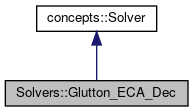
\includegraphics[width=217pt]{class_solvers_1_1_glutton___e_c_a___dec__inherit__graph}
\end{center}
\end{figure}


Collaboration diagram for Solvers\+:\+:Glutton\+\_\+\+E\+C\+A\+\_\+\+Dec\+:\nopagebreak
\begin{figure}[H]
\begin{center}
\leavevmode
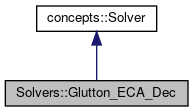
\includegraphics[width=217pt]{class_solvers_1_1_glutton___e_c_a___dec__coll__graph}
\end{center}
\end{figure}
\subsection*{Public Member Functions}
\begin{DoxyCompactItemize}
\item 
\hyperlink{class_solvers_1_1_glutton___e_c_a___dec_a4afb4df597dd89d1b24bc1def390b829}{Glutton\+\_\+\+E\+C\+A\+\_\+\+Dec} ()
\item 
\hyperlink{class_solvers_1_1_glutton___e_c_a___dec}{Glutton\+\_\+\+E\+C\+A\+\_\+\+Dec} \& \hyperlink{class_solvers_1_1_glutton___e_c_a___dec_ac00e2e76cc44f814db12a5ddea0177f3}{set\+Log\+Level} (int log\+\_\+level)
\item 
\hyperlink{class_solvers_1_1_glutton___e_c_a___dec}{Glutton\+\_\+\+E\+C\+A\+\_\+\+Dec} \& \hyperlink{class_solvers_1_1_glutton___e_c_a___dec_ad91bf6be2581ac099127ed4fe5248210}{set\+Parallel} (int parallel)
\item 
\hyperlink{class_solution}{Solution} $\ast$ \hyperlink{class_solvers_1_1_glutton___e_c_a___dec_a6b7078518779722dfaed6b1b1a9ba502}{solve} (const \hyperlink{class_landscape}{Landscape} \&landscape, const \hyperlink{class_restoration_plan}{Restoration\+Plan} \&plan, const double B) const
\item 
const std\+::string \hyperlink{class_solvers_1_1_glutton___e_c_a___dec_a2990dbcfecba9673d4bbae331aee1a04}{name} () const
\end{DoxyCompactItemize}
\subsection*{Additional Inherited Members}


\subsection{Constructor \& Destructor Documentation}
\mbox{\Hypertarget{class_solvers_1_1_glutton___e_c_a___dec_a4afb4df597dd89d1b24bc1def390b829}\label{class_solvers_1_1_glutton___e_c_a___dec_a4afb4df597dd89d1b24bc1def390b829}} 
\index{Solvers\+::\+Glutton\+\_\+\+E\+C\+A\+\_\+\+Dec@{Solvers\+::\+Glutton\+\_\+\+E\+C\+A\+\_\+\+Dec}!Glutton\+\_\+\+E\+C\+A\+\_\+\+Dec@{Glutton\+\_\+\+E\+C\+A\+\_\+\+Dec}}
\index{Glutton\+\_\+\+E\+C\+A\+\_\+\+Dec@{Glutton\+\_\+\+E\+C\+A\+\_\+\+Dec}!Solvers\+::\+Glutton\+\_\+\+E\+C\+A\+\_\+\+Dec@{Solvers\+::\+Glutton\+\_\+\+E\+C\+A\+\_\+\+Dec}}
\subsubsection{\texorpdfstring{Glutton\+\_\+\+E\+C\+A\+\_\+\+Dec()}{Glutton\_ECA\_Dec()}}
{\footnotesize\ttfamily Solvers\+::\+Glutton\+\_\+\+E\+C\+A\+\_\+\+Dec\+::\+Glutton\+\_\+\+E\+C\+A\+\_\+\+Dec (\begin{DoxyParamCaption}{ }\end{DoxyParamCaption})\hspace{0.3cm}{\ttfamily [inline]}}



\subsection{Member Function Documentation}
\mbox{\Hypertarget{class_solvers_1_1_glutton___e_c_a___dec_a2990dbcfecba9673d4bbae331aee1a04}\label{class_solvers_1_1_glutton___e_c_a___dec_a2990dbcfecba9673d4bbae331aee1a04}} 
\index{Solvers\+::\+Glutton\+\_\+\+E\+C\+A\+\_\+\+Dec@{Solvers\+::\+Glutton\+\_\+\+E\+C\+A\+\_\+\+Dec}!name@{name}}
\index{name@{name}!Solvers\+::\+Glutton\+\_\+\+E\+C\+A\+\_\+\+Dec@{Solvers\+::\+Glutton\+\_\+\+E\+C\+A\+\_\+\+Dec}}
\subsubsection{\texorpdfstring{name()}{name()}}
{\footnotesize\ttfamily const std\+::string Solvers\+::\+Glutton\+\_\+\+E\+C\+A\+\_\+\+Dec\+::name (\begin{DoxyParamCaption}{ }\end{DoxyParamCaption}) const\hspace{0.3cm}{\ttfamily [inline]}, {\ttfamily [virtual]}}



Implements \hyperlink{classconcepts_1_1_solver_ab995568318a506446228f45cab2fcce7}{concepts\+::\+Solver}.

\mbox{\Hypertarget{class_solvers_1_1_glutton___e_c_a___dec_ac00e2e76cc44f814db12a5ddea0177f3}\label{class_solvers_1_1_glutton___e_c_a___dec_ac00e2e76cc44f814db12a5ddea0177f3}} 
\index{Solvers\+::\+Glutton\+\_\+\+E\+C\+A\+\_\+\+Dec@{Solvers\+::\+Glutton\+\_\+\+E\+C\+A\+\_\+\+Dec}!set\+Log\+Level@{set\+Log\+Level}}
\index{set\+Log\+Level@{set\+Log\+Level}!Solvers\+::\+Glutton\+\_\+\+E\+C\+A\+\_\+\+Dec@{Solvers\+::\+Glutton\+\_\+\+E\+C\+A\+\_\+\+Dec}}
\subsubsection{\texorpdfstring{set\+Log\+Level()}{setLogLevel()}}
{\footnotesize\ttfamily \hyperlink{class_solvers_1_1_glutton___e_c_a___dec}{Glutton\+\_\+\+E\+C\+A\+\_\+\+Dec}\& Solvers\+::\+Glutton\+\_\+\+E\+C\+A\+\_\+\+Dec\+::set\+Log\+Level (\begin{DoxyParamCaption}\item[{int}]{log\+\_\+level }\end{DoxyParamCaption})\hspace{0.3cm}{\ttfamily [inline]}}

\mbox{\Hypertarget{class_solvers_1_1_glutton___e_c_a___dec_ad91bf6be2581ac099127ed4fe5248210}\label{class_solvers_1_1_glutton___e_c_a___dec_ad91bf6be2581ac099127ed4fe5248210}} 
\index{Solvers\+::\+Glutton\+\_\+\+E\+C\+A\+\_\+\+Dec@{Solvers\+::\+Glutton\+\_\+\+E\+C\+A\+\_\+\+Dec}!set\+Parallel@{set\+Parallel}}
\index{set\+Parallel@{set\+Parallel}!Solvers\+::\+Glutton\+\_\+\+E\+C\+A\+\_\+\+Dec@{Solvers\+::\+Glutton\+\_\+\+E\+C\+A\+\_\+\+Dec}}
\subsubsection{\texorpdfstring{set\+Parallel()}{setParallel()}}
{\footnotesize\ttfamily \hyperlink{class_solvers_1_1_glutton___e_c_a___dec}{Glutton\+\_\+\+E\+C\+A\+\_\+\+Dec}\& Solvers\+::\+Glutton\+\_\+\+E\+C\+A\+\_\+\+Dec\+::set\+Parallel (\begin{DoxyParamCaption}\item[{int}]{parallel }\end{DoxyParamCaption})\hspace{0.3cm}{\ttfamily [inline]}}

\mbox{\Hypertarget{class_solvers_1_1_glutton___e_c_a___dec_a6b7078518779722dfaed6b1b1a9ba502}\label{class_solvers_1_1_glutton___e_c_a___dec_a6b7078518779722dfaed6b1b1a9ba502}} 
\index{Solvers\+::\+Glutton\+\_\+\+E\+C\+A\+\_\+\+Dec@{Solvers\+::\+Glutton\+\_\+\+E\+C\+A\+\_\+\+Dec}!solve@{solve}}
\index{solve@{solve}!Solvers\+::\+Glutton\+\_\+\+E\+C\+A\+\_\+\+Dec@{Solvers\+::\+Glutton\+\_\+\+E\+C\+A\+\_\+\+Dec}}
\subsubsection{\texorpdfstring{solve()}{solve()}}
{\footnotesize\ttfamily \hyperlink{class_solution}{Solution} $\ast$ Solvers\+::\+Glutton\+\_\+\+E\+C\+A\+\_\+\+Dec\+::solve (\begin{DoxyParamCaption}\item[{const \hyperlink{class_landscape}{Landscape} \&}]{landscape,  }\item[{const \hyperlink{class_restoration_plan}{Restoration\+Plan} \&}]{plan,  }\item[{const double}]{B }\end{DoxyParamCaption}) const\hspace{0.3cm}{\ttfamily [virtual]}}



Implements \hyperlink{classconcepts_1_1_solver_af323ad29df1e7b87facd7dc007568c80}{concepts\+::\+Solver}.



The documentation for this class was generated from the following files\+:\begin{DoxyCompactItemize}
\item 
/home/plaiseek/\+Projects/landscape\+\_\+opt\+\_\+cpp/include/solvers/\hyperlink{glutton__eca__dec_8hpp}{glutton\+\_\+eca\+\_\+dec.\+hpp}\item 
/home/plaiseek/\+Projects/landscape\+\_\+opt\+\_\+cpp/src/solvers/\hyperlink{glutton__eca__dec_8cpp}{glutton\+\_\+eca\+\_\+dec.\+cpp}\end{DoxyCompactItemize}

\hypertarget{class_solvers_1_1_glutton___e_c_a___inc}{}\section{Solvers\+:\+:Glutton\+\_\+\+E\+C\+A\+\_\+\+Inc Class Reference}
\label{class_solvers_1_1_glutton___e_c_a___inc}\index{Solvers\+::\+Glutton\+\_\+\+E\+C\+A\+\_\+\+Inc@{Solvers\+::\+Glutton\+\_\+\+E\+C\+A\+\_\+\+Inc}}


{\ttfamily \#include $<$glutton\+\_\+eca\+\_\+inc.\+hpp$>$}



Inheritance diagram for Solvers\+:\+:Glutton\+\_\+\+E\+C\+A\+\_\+\+Inc\+:\nopagebreak
\begin{figure}[H]
\begin{center}
\leavevmode
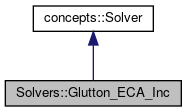
\includegraphics[width=212pt]{class_solvers_1_1_glutton___e_c_a___inc__inherit__graph}
\end{center}
\end{figure}


Collaboration diagram for Solvers\+:\+:Glutton\+\_\+\+E\+C\+A\+\_\+\+Inc\+:\nopagebreak
\begin{figure}[H]
\begin{center}
\leavevmode
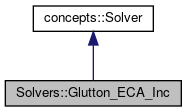
\includegraphics[width=212pt]{class_solvers_1_1_glutton___e_c_a___inc__coll__graph}
\end{center}
\end{figure}
\subsection*{Public Member Functions}
\begin{DoxyCompactItemize}
\item 
\hyperlink{class_solvers_1_1_glutton___e_c_a___inc_a60d52fd5046feb707fc3169c783a9bbd}{Glutton\+\_\+\+E\+C\+A\+\_\+\+Inc} ()
\item 
\hyperlink{class_solvers_1_1_glutton___e_c_a___inc}{Glutton\+\_\+\+E\+C\+A\+\_\+\+Inc} \& \hyperlink{class_solvers_1_1_glutton___e_c_a___inc_ac8d3d5fa78d9f2580d632f5d2488e496}{set\+Log\+Level} (int log\+\_\+level)
\item 
\hyperlink{class_solvers_1_1_glutton___e_c_a___inc}{Glutton\+\_\+\+E\+C\+A\+\_\+\+Inc} \& \hyperlink{class_solvers_1_1_glutton___e_c_a___inc_a6ea2e16e8ec0a549b8889e5c994bb593}{set\+Parallel} (int parallel)
\item 
\hyperlink{class_solution}{Solution} $\ast$ \hyperlink{class_solvers_1_1_glutton___e_c_a___inc_a12c872bf34761d875649f3e029dbc952}{solve} (const \hyperlink{class_landscape}{Landscape} \&landscape, const \hyperlink{class_restoration_plan}{Restoration\+Plan} \&plan, const double B) const
\item 
const std\+::string \hyperlink{class_solvers_1_1_glutton___e_c_a___inc_afda6b975b3a066aa76711730e5fa2f48}{name} () const
\end{DoxyCompactItemize}
\subsection*{Additional Inherited Members}


\subsection{Constructor \& Destructor Documentation}
\mbox{\Hypertarget{class_solvers_1_1_glutton___e_c_a___inc_a60d52fd5046feb707fc3169c783a9bbd}\label{class_solvers_1_1_glutton___e_c_a___inc_a60d52fd5046feb707fc3169c783a9bbd}} 
\index{Solvers\+::\+Glutton\+\_\+\+E\+C\+A\+\_\+\+Inc@{Solvers\+::\+Glutton\+\_\+\+E\+C\+A\+\_\+\+Inc}!Glutton\+\_\+\+E\+C\+A\+\_\+\+Inc@{Glutton\+\_\+\+E\+C\+A\+\_\+\+Inc}}
\index{Glutton\+\_\+\+E\+C\+A\+\_\+\+Inc@{Glutton\+\_\+\+E\+C\+A\+\_\+\+Inc}!Solvers\+::\+Glutton\+\_\+\+E\+C\+A\+\_\+\+Inc@{Solvers\+::\+Glutton\+\_\+\+E\+C\+A\+\_\+\+Inc}}
\subsubsection{\texorpdfstring{Glutton\+\_\+\+E\+C\+A\+\_\+\+Inc()}{Glutton\_ECA\_Inc()}}
{\footnotesize\ttfamily Solvers\+::\+Glutton\+\_\+\+E\+C\+A\+\_\+\+Inc\+::\+Glutton\+\_\+\+E\+C\+A\+\_\+\+Inc (\begin{DoxyParamCaption}{ }\end{DoxyParamCaption})\hspace{0.3cm}{\ttfamily [inline]}}



\subsection{Member Function Documentation}
\mbox{\Hypertarget{class_solvers_1_1_glutton___e_c_a___inc_afda6b975b3a066aa76711730e5fa2f48}\label{class_solvers_1_1_glutton___e_c_a___inc_afda6b975b3a066aa76711730e5fa2f48}} 
\index{Solvers\+::\+Glutton\+\_\+\+E\+C\+A\+\_\+\+Inc@{Solvers\+::\+Glutton\+\_\+\+E\+C\+A\+\_\+\+Inc}!name@{name}}
\index{name@{name}!Solvers\+::\+Glutton\+\_\+\+E\+C\+A\+\_\+\+Inc@{Solvers\+::\+Glutton\+\_\+\+E\+C\+A\+\_\+\+Inc}}
\subsubsection{\texorpdfstring{name()}{name()}}
{\footnotesize\ttfamily const std\+::string Solvers\+::\+Glutton\+\_\+\+E\+C\+A\+\_\+\+Inc\+::name (\begin{DoxyParamCaption}{ }\end{DoxyParamCaption}) const\hspace{0.3cm}{\ttfamily [inline]}, {\ttfamily [virtual]}}



Implements \hyperlink{classconcepts_1_1_solver_ab995568318a506446228f45cab2fcce7}{concepts\+::\+Solver}.

\mbox{\Hypertarget{class_solvers_1_1_glutton___e_c_a___inc_ac8d3d5fa78d9f2580d632f5d2488e496}\label{class_solvers_1_1_glutton___e_c_a___inc_ac8d3d5fa78d9f2580d632f5d2488e496}} 
\index{Solvers\+::\+Glutton\+\_\+\+E\+C\+A\+\_\+\+Inc@{Solvers\+::\+Glutton\+\_\+\+E\+C\+A\+\_\+\+Inc}!set\+Log\+Level@{set\+Log\+Level}}
\index{set\+Log\+Level@{set\+Log\+Level}!Solvers\+::\+Glutton\+\_\+\+E\+C\+A\+\_\+\+Inc@{Solvers\+::\+Glutton\+\_\+\+E\+C\+A\+\_\+\+Inc}}
\subsubsection{\texorpdfstring{set\+Log\+Level()}{setLogLevel()}}
{\footnotesize\ttfamily \hyperlink{class_solvers_1_1_glutton___e_c_a___inc}{Glutton\+\_\+\+E\+C\+A\+\_\+\+Inc}\& Solvers\+::\+Glutton\+\_\+\+E\+C\+A\+\_\+\+Inc\+::set\+Log\+Level (\begin{DoxyParamCaption}\item[{int}]{log\+\_\+level }\end{DoxyParamCaption})\hspace{0.3cm}{\ttfamily [inline]}}

\mbox{\Hypertarget{class_solvers_1_1_glutton___e_c_a___inc_a6ea2e16e8ec0a549b8889e5c994bb593}\label{class_solvers_1_1_glutton___e_c_a___inc_a6ea2e16e8ec0a549b8889e5c994bb593}} 
\index{Solvers\+::\+Glutton\+\_\+\+E\+C\+A\+\_\+\+Inc@{Solvers\+::\+Glutton\+\_\+\+E\+C\+A\+\_\+\+Inc}!set\+Parallel@{set\+Parallel}}
\index{set\+Parallel@{set\+Parallel}!Solvers\+::\+Glutton\+\_\+\+E\+C\+A\+\_\+\+Inc@{Solvers\+::\+Glutton\+\_\+\+E\+C\+A\+\_\+\+Inc}}
\subsubsection{\texorpdfstring{set\+Parallel()}{setParallel()}}
{\footnotesize\ttfamily \hyperlink{class_solvers_1_1_glutton___e_c_a___inc}{Glutton\+\_\+\+E\+C\+A\+\_\+\+Inc}\& Solvers\+::\+Glutton\+\_\+\+E\+C\+A\+\_\+\+Inc\+::set\+Parallel (\begin{DoxyParamCaption}\item[{int}]{parallel }\end{DoxyParamCaption})\hspace{0.3cm}{\ttfamily [inline]}}

\mbox{\Hypertarget{class_solvers_1_1_glutton___e_c_a___inc_a12c872bf34761d875649f3e029dbc952}\label{class_solvers_1_1_glutton___e_c_a___inc_a12c872bf34761d875649f3e029dbc952}} 
\index{Solvers\+::\+Glutton\+\_\+\+E\+C\+A\+\_\+\+Inc@{Solvers\+::\+Glutton\+\_\+\+E\+C\+A\+\_\+\+Inc}!solve@{solve}}
\index{solve@{solve}!Solvers\+::\+Glutton\+\_\+\+E\+C\+A\+\_\+\+Inc@{Solvers\+::\+Glutton\+\_\+\+E\+C\+A\+\_\+\+Inc}}
\subsubsection{\texorpdfstring{solve()}{solve()}}
{\footnotesize\ttfamily \hyperlink{class_solution}{Solution} $\ast$ Solvers\+::\+Glutton\+\_\+\+E\+C\+A\+\_\+\+Inc\+::solve (\begin{DoxyParamCaption}\item[{const \hyperlink{class_landscape}{Landscape} \&}]{landscape,  }\item[{const \hyperlink{class_restoration_plan}{Restoration\+Plan} \&}]{plan,  }\item[{const double}]{B }\end{DoxyParamCaption}) const\hspace{0.3cm}{\ttfamily [virtual]}}



Implements \hyperlink{classconcepts_1_1_solver_af323ad29df1e7b87facd7dc007568c80}{concepts\+::\+Solver}.



The documentation for this class was generated from the following files\+:\begin{DoxyCompactItemize}
\item 
/home/plaiseek/\+Projects/landscape\+\_\+opt\+\_\+cpp/include/solvers/\hyperlink{glutton__eca__inc_8hpp}{glutton\+\_\+eca\+\_\+inc.\+hpp}\item 
/home/plaiseek/\+Projects/landscape\+\_\+opt\+\_\+cpp/src/solvers/\hyperlink{glutton__eca__inc_8cpp}{glutton\+\_\+eca\+\_\+inc.\+cpp}\end{DoxyCompactItemize}

\hypertarget{structlemon_1_1_identify_default_traits}{}\section{lemon\+:\+:Identify\+Default\+Traits$<$ GR, L\+EN $>$ Struct Template Reference}
\label{structlemon_1_1_identify_default_traits}\index{lemon\+::\+Identify\+Default\+Traits$<$ G\+R, L\+E\+N $>$@{lemon\+::\+Identify\+Default\+Traits$<$ G\+R, L\+E\+N $>$}}


{\ttfamily \#include $<$identify\+\_\+strong\+\_\+arcs.\+h$>$}

\subsection*{Public Types}
\begin{DoxyCompactItemize}
\item 
typedef GR \hyperlink{structlemon_1_1_identify_default_traits_a5fddb27be8d17b86b2c4f94e72b8a8da}{Digraph}
\item 
typedef L\+EN \hyperlink{structlemon_1_1_identify_default_traits_a1edc74d982d4d9b918cffcf2ba6b5ec7}{Length\+Map}
\item 
typedef L\+E\+N\+::\+Value \hyperlink{structlemon_1_1_identify_default_traits_ae44641190d3358bbe94ff53a18c36193}{Value}
\item 
typedef \hyperlink{classlemon_1_1_labeled_value}{Labeled\+Value}$<$ \hyperlink{structlemon_1_1_identify_default_traits_ae44641190d3358bbe94ff53a18c36193}{Value} $>$ \hyperlink{structlemon_1_1_identify_default_traits_a6f612abe02956f7a3c607e882d7e8d87}{Labeled\+Dist}
\item 
typedef Dijkstra\+Default\+Operation\+Traits$<$ \hyperlink{structlemon_1_1_identify_default_traits_a6f612abe02956f7a3c607e882d7e8d87}{Labeled\+Dist} $>$ \hyperlink{structlemon_1_1_identify_default_traits_acde989e160acfe85bc44e3e0a1c257fe}{Operation\+Traits}
\item 
typedef Digraph\+::template Node\+Map$<$ int $>$ \hyperlink{structlemon_1_1_identify_default_traits_a05e9c5d0e980eb5f75a09449fc7d597f}{Heap\+Cross\+Ref}
\item 
typedef Bin\+Heap$<$ \hyperlink{structlemon_1_1_identify_default_traits_a6f612abe02956f7a3c607e882d7e8d87}{Labeled\+Dist}, \hyperlink{structlemon_1_1_identify_default_traits_a05e9c5d0e980eb5f75a09449fc7d597f}{Heap\+Cross\+Ref}, std\+::less$<$ \hyperlink{structlemon_1_1_identify_default_traits_a6f612abe02956f7a3c607e882d7e8d87}{Labeled\+Dist} $>$ $>$ \hyperlink{structlemon_1_1_identify_default_traits_abb89b2848e63f4cb0712ca701db72aa4}{Heap}
\item 
typedef Digraph\+::\+Node \hyperlink{structlemon_1_1_identify_default_traits_a8cd1d66e1f5de579d028a3b18561ea5a}{Node}
\item 
typedef std\+::vector$<$ \hyperlink{structlemon_1_1_identify_default_traits_a8cd1d66e1f5de579d028a3b18561ea5a}{Node} $>$ \hyperlink{structlemon_1_1_identify_default_traits_ac7ceaa832e1553cd7fda8d3edc14023e}{Node\+List}
\end{DoxyCompactItemize}
\subsection*{Static Public Member Functions}
\begin{DoxyCompactItemize}
\item 
static \hyperlink{structlemon_1_1_identify_default_traits_a05e9c5d0e980eb5f75a09449fc7d597f}{Heap\+Cross\+Ref} $\ast$ \hyperlink{structlemon_1_1_identify_default_traits_a17ee2bd5691be1d00565f999fec63d47}{create\+Heap\+Cross\+Ref} (const \hyperlink{structlemon_1_1_identify_default_traits_a5fddb27be8d17b86b2c4f94e72b8a8da}{Digraph} \&g)
\item 
static \hyperlink{structlemon_1_1_identify_default_traits_abb89b2848e63f4cb0712ca701db72aa4}{Heap} $\ast$ \hyperlink{structlemon_1_1_identify_default_traits_a28654afa585a6b293ebd0afaf78b4411}{create\+Heap} (\hyperlink{structlemon_1_1_identify_default_traits_a05e9c5d0e980eb5f75a09449fc7d597f}{Heap\+Cross\+Ref} \&r)
\item 
static \hyperlink{structlemon_1_1_identify_default_traits_ac7ceaa832e1553cd7fda8d3edc14023e}{Node\+List} $\ast$ \hyperlink{structlemon_1_1_identify_default_traits_a3c15b93174b21ed7afca1f2c20aac7bc}{create\+Node\+List} (const \hyperlink{structlemon_1_1_identify_default_traits_a5fddb27be8d17b86b2c4f94e72b8a8da}{Digraph} \&)
\item 
static void \hyperlink{structlemon_1_1_identify_default_traits_aa127d5835d6adf71c52ef3806d8d3e2d}{add\+Node} (\hyperlink{structlemon_1_1_identify_default_traits_ac7ceaa832e1553cd7fda8d3edc14023e}{Node\+List} \&n, \hyperlink{structlemon_1_1_identify_default_traits_a8cd1d66e1f5de579d028a3b18561ea5a}{Node} u)
\end{DoxyCompactItemize}


\subsection{Member Typedef Documentation}
\mbox{\Hypertarget{structlemon_1_1_identify_default_traits_a5fddb27be8d17b86b2c4f94e72b8a8da}\label{structlemon_1_1_identify_default_traits_a5fddb27be8d17b86b2c4f94e72b8a8da}} 
\index{lemon\+::\+Identify\+Default\+Traits@{lemon\+::\+Identify\+Default\+Traits}!Digraph@{Digraph}}
\index{Digraph@{Digraph}!lemon\+::\+Identify\+Default\+Traits@{lemon\+::\+Identify\+Default\+Traits}}
\subsubsection{\texorpdfstring{Digraph}{Digraph}}
{\footnotesize\ttfamily template$<$typename GR , typename L\+EN $>$ \\
typedef GR \hyperlink{structlemon_1_1_identify_default_traits}{lemon\+::\+Identify\+Default\+Traits}$<$ GR, L\+EN $>$\+::\hyperlink{structlemon_1_1_identify_default_traits_a5fddb27be8d17b86b2c4f94e72b8a8da}{Digraph}}

\mbox{\Hypertarget{structlemon_1_1_identify_default_traits_abb89b2848e63f4cb0712ca701db72aa4}\label{structlemon_1_1_identify_default_traits_abb89b2848e63f4cb0712ca701db72aa4}} 
\index{lemon\+::\+Identify\+Default\+Traits@{lemon\+::\+Identify\+Default\+Traits}!Heap@{Heap}}
\index{Heap@{Heap}!lemon\+::\+Identify\+Default\+Traits@{lemon\+::\+Identify\+Default\+Traits}}
\subsubsection{\texorpdfstring{Heap}{Heap}}
{\footnotesize\ttfamily template$<$typename GR , typename L\+EN $>$ \\
typedef Bin\+Heap$<$\hyperlink{structlemon_1_1_identify_default_traits_a6f612abe02956f7a3c607e882d7e8d87}{Labeled\+Dist}, \hyperlink{structlemon_1_1_identify_default_traits_a05e9c5d0e980eb5f75a09449fc7d597f}{Heap\+Cross\+Ref}, std\+::less$<$\hyperlink{structlemon_1_1_identify_default_traits_a6f612abe02956f7a3c607e882d7e8d87}{Labeled\+Dist}$>$ $>$ \hyperlink{structlemon_1_1_identify_default_traits}{lemon\+::\+Identify\+Default\+Traits}$<$ GR, L\+EN $>$\+::\hyperlink{structlemon_1_1_identify_default_traits_abb89b2848e63f4cb0712ca701db72aa4}{Heap}}

\mbox{\Hypertarget{structlemon_1_1_identify_default_traits_a05e9c5d0e980eb5f75a09449fc7d597f}\label{structlemon_1_1_identify_default_traits_a05e9c5d0e980eb5f75a09449fc7d597f}} 
\index{lemon\+::\+Identify\+Default\+Traits@{lemon\+::\+Identify\+Default\+Traits}!Heap\+Cross\+Ref@{Heap\+Cross\+Ref}}
\index{Heap\+Cross\+Ref@{Heap\+Cross\+Ref}!lemon\+::\+Identify\+Default\+Traits@{lemon\+::\+Identify\+Default\+Traits}}
\subsubsection{\texorpdfstring{Heap\+Cross\+Ref}{HeapCrossRef}}
{\footnotesize\ttfamily template$<$typename GR , typename L\+EN $>$ \\
typedef Digraph\+::template Node\+Map$<$int$>$ \hyperlink{structlemon_1_1_identify_default_traits}{lemon\+::\+Identify\+Default\+Traits}$<$ GR, L\+EN $>$\+::\hyperlink{structlemon_1_1_identify_default_traits_a05e9c5d0e980eb5f75a09449fc7d597f}{Heap\+Cross\+Ref}}

\mbox{\Hypertarget{structlemon_1_1_identify_default_traits_a6f612abe02956f7a3c607e882d7e8d87}\label{structlemon_1_1_identify_default_traits_a6f612abe02956f7a3c607e882d7e8d87}} 
\index{lemon\+::\+Identify\+Default\+Traits@{lemon\+::\+Identify\+Default\+Traits}!Labeled\+Dist@{Labeled\+Dist}}
\index{Labeled\+Dist@{Labeled\+Dist}!lemon\+::\+Identify\+Default\+Traits@{lemon\+::\+Identify\+Default\+Traits}}
\subsubsection{\texorpdfstring{Labeled\+Dist}{LabeledDist}}
{\footnotesize\ttfamily template$<$typename GR , typename L\+EN $>$ \\
typedef \hyperlink{classlemon_1_1_labeled_value}{Labeled\+Value}$<$\hyperlink{structlemon_1_1_identify_default_traits_ae44641190d3358bbe94ff53a18c36193}{Value}$>$ \hyperlink{structlemon_1_1_identify_default_traits}{lemon\+::\+Identify\+Default\+Traits}$<$ GR, L\+EN $>$\+::\hyperlink{structlemon_1_1_identify_default_traits_a6f612abe02956f7a3c607e882d7e8d87}{Labeled\+Dist}}

\mbox{\Hypertarget{structlemon_1_1_identify_default_traits_a1edc74d982d4d9b918cffcf2ba6b5ec7}\label{structlemon_1_1_identify_default_traits_a1edc74d982d4d9b918cffcf2ba6b5ec7}} 
\index{lemon\+::\+Identify\+Default\+Traits@{lemon\+::\+Identify\+Default\+Traits}!Length\+Map@{Length\+Map}}
\index{Length\+Map@{Length\+Map}!lemon\+::\+Identify\+Default\+Traits@{lemon\+::\+Identify\+Default\+Traits}}
\subsubsection{\texorpdfstring{Length\+Map}{LengthMap}}
{\footnotesize\ttfamily template$<$typename GR , typename L\+EN $>$ \\
typedef L\+EN \hyperlink{structlemon_1_1_identify_default_traits}{lemon\+::\+Identify\+Default\+Traits}$<$ GR, L\+EN $>$\+::\hyperlink{structlemon_1_1_identify_default_traits_a1edc74d982d4d9b918cffcf2ba6b5ec7}{Length\+Map}}

\mbox{\Hypertarget{structlemon_1_1_identify_default_traits_a8cd1d66e1f5de579d028a3b18561ea5a}\label{structlemon_1_1_identify_default_traits_a8cd1d66e1f5de579d028a3b18561ea5a}} 
\index{lemon\+::\+Identify\+Default\+Traits@{lemon\+::\+Identify\+Default\+Traits}!Node@{Node}}
\index{Node@{Node}!lemon\+::\+Identify\+Default\+Traits@{lemon\+::\+Identify\+Default\+Traits}}
\subsubsection{\texorpdfstring{Node}{Node}}
{\footnotesize\ttfamily template$<$typename GR , typename L\+EN $>$ \\
typedef Digraph\+::\+Node \hyperlink{structlemon_1_1_identify_default_traits}{lemon\+::\+Identify\+Default\+Traits}$<$ GR, L\+EN $>$\+::\hyperlink{structlemon_1_1_identify_default_traits_a8cd1d66e1f5de579d028a3b18561ea5a}{Node}}

\mbox{\Hypertarget{structlemon_1_1_identify_default_traits_ac7ceaa832e1553cd7fda8d3edc14023e}\label{structlemon_1_1_identify_default_traits_ac7ceaa832e1553cd7fda8d3edc14023e}} 
\index{lemon\+::\+Identify\+Default\+Traits@{lemon\+::\+Identify\+Default\+Traits}!Node\+List@{Node\+List}}
\index{Node\+List@{Node\+List}!lemon\+::\+Identify\+Default\+Traits@{lemon\+::\+Identify\+Default\+Traits}}
\subsubsection{\texorpdfstring{Node\+List}{NodeList}}
{\footnotesize\ttfamily template$<$typename GR , typename L\+EN $>$ \\
typedef std\+::vector$<$\hyperlink{structlemon_1_1_identify_default_traits_a8cd1d66e1f5de579d028a3b18561ea5a}{Node}$>$ \hyperlink{structlemon_1_1_identify_default_traits}{lemon\+::\+Identify\+Default\+Traits}$<$ GR, L\+EN $>$\+::\hyperlink{structlemon_1_1_identify_default_traits_ac7ceaa832e1553cd7fda8d3edc14023e}{Node\+List}}

\mbox{\Hypertarget{structlemon_1_1_identify_default_traits_acde989e160acfe85bc44e3e0a1c257fe}\label{structlemon_1_1_identify_default_traits_acde989e160acfe85bc44e3e0a1c257fe}} 
\index{lemon\+::\+Identify\+Default\+Traits@{lemon\+::\+Identify\+Default\+Traits}!Operation\+Traits@{Operation\+Traits}}
\index{Operation\+Traits@{Operation\+Traits}!lemon\+::\+Identify\+Default\+Traits@{lemon\+::\+Identify\+Default\+Traits}}
\subsubsection{\texorpdfstring{Operation\+Traits}{OperationTraits}}
{\footnotesize\ttfamily template$<$typename GR , typename L\+EN $>$ \\
typedef Dijkstra\+Default\+Operation\+Traits$<$\hyperlink{structlemon_1_1_identify_default_traits_a6f612abe02956f7a3c607e882d7e8d87}{Labeled\+Dist}$>$ \hyperlink{structlemon_1_1_identify_default_traits}{lemon\+::\+Identify\+Default\+Traits}$<$ GR, L\+EN $>$\+::\hyperlink{structlemon_1_1_identify_default_traits_acde989e160acfe85bc44e3e0a1c257fe}{Operation\+Traits}}

\mbox{\Hypertarget{structlemon_1_1_identify_default_traits_ae44641190d3358bbe94ff53a18c36193}\label{structlemon_1_1_identify_default_traits_ae44641190d3358bbe94ff53a18c36193}} 
\index{lemon\+::\+Identify\+Default\+Traits@{lemon\+::\+Identify\+Default\+Traits}!Value@{Value}}
\index{Value@{Value}!lemon\+::\+Identify\+Default\+Traits@{lemon\+::\+Identify\+Default\+Traits}}
\subsubsection{\texorpdfstring{Value}{Value}}
{\footnotesize\ttfamily template$<$typename GR , typename L\+EN $>$ \\
typedef L\+E\+N\+::\+Value \hyperlink{structlemon_1_1_identify_default_traits}{lemon\+::\+Identify\+Default\+Traits}$<$ GR, L\+EN $>$\+::\hyperlink{structlemon_1_1_identify_default_traits_ae44641190d3358bbe94ff53a18c36193}{Value}}



\subsection{Member Function Documentation}
\mbox{\Hypertarget{structlemon_1_1_identify_default_traits_aa127d5835d6adf71c52ef3806d8d3e2d}\label{structlemon_1_1_identify_default_traits_aa127d5835d6adf71c52ef3806d8d3e2d}} 
\index{lemon\+::\+Identify\+Default\+Traits@{lemon\+::\+Identify\+Default\+Traits}!add\+Node@{add\+Node}}
\index{add\+Node@{add\+Node}!lemon\+::\+Identify\+Default\+Traits@{lemon\+::\+Identify\+Default\+Traits}}
\subsubsection{\texorpdfstring{add\+Node()}{addNode()}}
{\footnotesize\ttfamily template$<$typename GR , typename L\+EN $>$ \\
static void \hyperlink{structlemon_1_1_identify_default_traits}{lemon\+::\+Identify\+Default\+Traits}$<$ GR, L\+EN $>$\+::add\+Node (\begin{DoxyParamCaption}\item[{\hyperlink{structlemon_1_1_identify_default_traits_ac7ceaa832e1553cd7fda8d3edc14023e}{Node\+List} \&}]{n,  }\item[{\hyperlink{structlemon_1_1_identify_default_traits_a8cd1d66e1f5de579d028a3b18561ea5a}{Node}}]{u }\end{DoxyParamCaption})\hspace{0.3cm}{\ttfamily [inline]}, {\ttfamily [static]}}

\mbox{\Hypertarget{structlemon_1_1_identify_default_traits_a28654afa585a6b293ebd0afaf78b4411}\label{structlemon_1_1_identify_default_traits_a28654afa585a6b293ebd0afaf78b4411}} 
\index{lemon\+::\+Identify\+Default\+Traits@{lemon\+::\+Identify\+Default\+Traits}!create\+Heap@{create\+Heap}}
\index{create\+Heap@{create\+Heap}!lemon\+::\+Identify\+Default\+Traits@{lemon\+::\+Identify\+Default\+Traits}}
\subsubsection{\texorpdfstring{create\+Heap()}{createHeap()}}
{\footnotesize\ttfamily template$<$typename GR , typename L\+EN $>$ \\
static \hyperlink{structlemon_1_1_identify_default_traits_abb89b2848e63f4cb0712ca701db72aa4}{Heap}$\ast$ \hyperlink{structlemon_1_1_identify_default_traits}{lemon\+::\+Identify\+Default\+Traits}$<$ GR, L\+EN $>$\+::create\+Heap (\begin{DoxyParamCaption}\item[{\hyperlink{structlemon_1_1_identify_default_traits_a05e9c5d0e980eb5f75a09449fc7d597f}{Heap\+Cross\+Ref} \&}]{r }\end{DoxyParamCaption})\hspace{0.3cm}{\ttfamily [inline]}, {\ttfamily [static]}}

\mbox{\Hypertarget{structlemon_1_1_identify_default_traits_a17ee2bd5691be1d00565f999fec63d47}\label{structlemon_1_1_identify_default_traits_a17ee2bd5691be1d00565f999fec63d47}} 
\index{lemon\+::\+Identify\+Default\+Traits@{lemon\+::\+Identify\+Default\+Traits}!create\+Heap\+Cross\+Ref@{create\+Heap\+Cross\+Ref}}
\index{create\+Heap\+Cross\+Ref@{create\+Heap\+Cross\+Ref}!lemon\+::\+Identify\+Default\+Traits@{lemon\+::\+Identify\+Default\+Traits}}
\subsubsection{\texorpdfstring{create\+Heap\+Cross\+Ref()}{createHeapCrossRef()}}
{\footnotesize\ttfamily template$<$typename GR , typename L\+EN $>$ \\
static \hyperlink{structlemon_1_1_identify_default_traits_a05e9c5d0e980eb5f75a09449fc7d597f}{Heap\+Cross\+Ref}$\ast$ \hyperlink{structlemon_1_1_identify_default_traits}{lemon\+::\+Identify\+Default\+Traits}$<$ GR, L\+EN $>$\+::create\+Heap\+Cross\+Ref (\begin{DoxyParamCaption}\item[{const \hyperlink{structlemon_1_1_identify_default_traits_a5fddb27be8d17b86b2c4f94e72b8a8da}{Digraph} \&}]{g }\end{DoxyParamCaption})\hspace{0.3cm}{\ttfamily [inline]}, {\ttfamily [static]}}

\mbox{\Hypertarget{structlemon_1_1_identify_default_traits_a3c15b93174b21ed7afca1f2c20aac7bc}\label{structlemon_1_1_identify_default_traits_a3c15b93174b21ed7afca1f2c20aac7bc}} 
\index{lemon\+::\+Identify\+Default\+Traits@{lemon\+::\+Identify\+Default\+Traits}!create\+Node\+List@{create\+Node\+List}}
\index{create\+Node\+List@{create\+Node\+List}!lemon\+::\+Identify\+Default\+Traits@{lemon\+::\+Identify\+Default\+Traits}}
\subsubsection{\texorpdfstring{create\+Node\+List()}{createNodeList()}}
{\footnotesize\ttfamily template$<$typename GR , typename L\+EN $>$ \\
static \hyperlink{structlemon_1_1_identify_default_traits_ac7ceaa832e1553cd7fda8d3edc14023e}{Node\+List}$\ast$ \hyperlink{structlemon_1_1_identify_default_traits}{lemon\+::\+Identify\+Default\+Traits}$<$ GR, L\+EN $>$\+::create\+Node\+List (\begin{DoxyParamCaption}\item[{const \hyperlink{structlemon_1_1_identify_default_traits_a5fddb27be8d17b86b2c4f94e72b8a8da}{Digraph} \&}]{ }\end{DoxyParamCaption})\hspace{0.3cm}{\ttfamily [inline]}, {\ttfamily [static]}}



The documentation for this struct was generated from the following file\+:\begin{DoxyCompactItemize}
\item 
/home/plaiseek/\+Projects/landscape\+\_\+opt\+\_\+cpp/include/algorithms/\hyperlink{identify__strong__arcs_8h}{identify\+\_\+strong\+\_\+arcs.\+h}\end{DoxyCompactItemize}

\hypertarget{structlemon_1_1_identify_multiplicative_traits}{}\section{lemon\+:\+:Identify\+Multiplicative\+Traits$<$ GR, L\+EN $>$ Struct Template Reference}
\label{structlemon_1_1_identify_multiplicative_traits}\index{lemon\+::\+Identify\+Multiplicative\+Traits$<$ G\+R, L\+E\+N $>$@{lemon\+::\+Identify\+Multiplicative\+Traits$<$ G\+R, L\+E\+N $>$}}


{\ttfamily \#include $<$identify\+\_\+strong\+\_\+arcs.\+h$>$}

\subsection*{Public Types}
\begin{DoxyCompactItemize}
\item 
typedef GR \hyperlink{structlemon_1_1_identify_multiplicative_traits_a586c2b69092471f155318915c7e5bdd0}{Digraph}
\item 
typedef L\+EN \hyperlink{structlemon_1_1_identify_multiplicative_traits_a134355b88655b1c297264296d2c70d3a}{Length\+Map}
\item 
typedef L\+E\+N\+::\+Value \hyperlink{structlemon_1_1_identify_multiplicative_traits_ae44c59a817f36ac3d7c024fc75d5ae50}{Value}
\item 
typedef \hyperlink{classlemon_1_1_labeled_value}{Labeled\+Value}$<$ \hyperlink{structlemon_1_1_identify_multiplicative_traits_ae44c59a817f36ac3d7c024fc75d5ae50}{Value} $>$ \hyperlink{structlemon_1_1_identify_multiplicative_traits_a91b3da314fe157ce5c2674e3608d4cde}{Labeled\+Dist}
\item 
typedef \hyperlink{structlemon_1_1_dijkstra_multiplicative_operation_traits}{Dijkstra\+Multiplicative\+Operation\+Traits}$<$ \hyperlink{structlemon_1_1_identify_multiplicative_traits_a91b3da314fe157ce5c2674e3608d4cde}{Labeled\+Dist} $>$ \hyperlink{structlemon_1_1_identify_multiplicative_traits_ac66ce4af1205a7cd0564ad8d1ecf7a4a}{Operation\+Traits}
\item 
typedef Digraph\+::template Node\+Map$<$ int $>$ \hyperlink{structlemon_1_1_identify_multiplicative_traits_ae84c68f24215f7f666f26ca3125a284d}{Heap\+Cross\+Ref}
\item 
typedef Bin\+Heap$<$ \hyperlink{structlemon_1_1_identify_multiplicative_traits_a91b3da314fe157ce5c2674e3608d4cde}{Labeled\+Dist}, \hyperlink{structlemon_1_1_identify_multiplicative_traits_ae84c68f24215f7f666f26ca3125a284d}{Heap\+Cross\+Ref}, std\+::greater$<$ \hyperlink{structlemon_1_1_identify_multiplicative_traits_a91b3da314fe157ce5c2674e3608d4cde}{Labeled\+Dist} $>$ $>$ \hyperlink{structlemon_1_1_identify_multiplicative_traits_aa42c8b081b4e4783190eabd4ac03154f}{Heap}
\item 
typedef Digraph\+::\+Node \hyperlink{structlemon_1_1_identify_multiplicative_traits_a391c4d6be09a511224b23628fbc9c223}{Node}
\item 
typedef std\+::vector$<$ \hyperlink{structlemon_1_1_identify_multiplicative_traits_a391c4d6be09a511224b23628fbc9c223}{Node} $>$ \hyperlink{structlemon_1_1_identify_multiplicative_traits_a686335471dfcb3c0b7baef1764679a66}{Node\+List}
\end{DoxyCompactItemize}
\subsection*{Static Public Member Functions}
\begin{DoxyCompactItemize}
\item 
static \hyperlink{structlemon_1_1_identify_multiplicative_traits_ae84c68f24215f7f666f26ca3125a284d}{Heap\+Cross\+Ref} $\ast$ \hyperlink{structlemon_1_1_identify_multiplicative_traits_aeee352c508bf38e1994c9f22052c0be8}{create\+Heap\+Cross\+Ref} (const \hyperlink{structlemon_1_1_identify_multiplicative_traits_a586c2b69092471f155318915c7e5bdd0}{Digraph} \&g)
\item 
static \hyperlink{structlemon_1_1_identify_multiplicative_traits_aa42c8b081b4e4783190eabd4ac03154f}{Heap} $\ast$ \hyperlink{structlemon_1_1_identify_multiplicative_traits_af8070d2658718ee55c51790c25196235}{create\+Heap} (\hyperlink{structlemon_1_1_identify_multiplicative_traits_ae84c68f24215f7f666f26ca3125a284d}{Heap\+Cross\+Ref} \&r)
\item 
static \hyperlink{structlemon_1_1_identify_multiplicative_traits_a686335471dfcb3c0b7baef1764679a66}{Node\+List} $\ast$ \hyperlink{structlemon_1_1_identify_multiplicative_traits_a4a44286cb2877fb94d45d8ed0752c407}{create\+Node\+List} (const \hyperlink{structlemon_1_1_identify_multiplicative_traits_a586c2b69092471f155318915c7e5bdd0}{Digraph} \&)
\item 
static void \hyperlink{structlemon_1_1_identify_multiplicative_traits_afb385c6c785e4fd909345d8c37fe57a7}{add\+Node} (\hyperlink{structlemon_1_1_identify_multiplicative_traits_a686335471dfcb3c0b7baef1764679a66}{Node\+List} \&n, \hyperlink{structlemon_1_1_identify_multiplicative_traits_a391c4d6be09a511224b23628fbc9c223}{Node} u)
\end{DoxyCompactItemize}


\subsection{Member Typedef Documentation}
\mbox{\Hypertarget{structlemon_1_1_identify_multiplicative_traits_a586c2b69092471f155318915c7e5bdd0}\label{structlemon_1_1_identify_multiplicative_traits_a586c2b69092471f155318915c7e5bdd0}} 
\index{lemon\+::\+Identify\+Multiplicative\+Traits@{lemon\+::\+Identify\+Multiplicative\+Traits}!Digraph@{Digraph}}
\index{Digraph@{Digraph}!lemon\+::\+Identify\+Multiplicative\+Traits@{lemon\+::\+Identify\+Multiplicative\+Traits}}
\subsubsection{\texorpdfstring{Digraph}{Digraph}}
{\footnotesize\ttfamily template$<$typename GR , typename L\+EN $>$ \\
typedef GR \hyperlink{structlemon_1_1_identify_multiplicative_traits}{lemon\+::\+Identify\+Multiplicative\+Traits}$<$ GR, L\+EN $>$\+::\hyperlink{structlemon_1_1_identify_multiplicative_traits_a586c2b69092471f155318915c7e5bdd0}{Digraph}}

\mbox{\Hypertarget{structlemon_1_1_identify_multiplicative_traits_aa42c8b081b4e4783190eabd4ac03154f}\label{structlemon_1_1_identify_multiplicative_traits_aa42c8b081b4e4783190eabd4ac03154f}} 
\index{lemon\+::\+Identify\+Multiplicative\+Traits@{lemon\+::\+Identify\+Multiplicative\+Traits}!Heap@{Heap}}
\index{Heap@{Heap}!lemon\+::\+Identify\+Multiplicative\+Traits@{lemon\+::\+Identify\+Multiplicative\+Traits}}
\subsubsection{\texorpdfstring{Heap}{Heap}}
{\footnotesize\ttfamily template$<$typename GR , typename L\+EN $>$ \\
typedef Bin\+Heap$<$\hyperlink{structlemon_1_1_identify_multiplicative_traits_a91b3da314fe157ce5c2674e3608d4cde}{Labeled\+Dist}, \hyperlink{structlemon_1_1_identify_multiplicative_traits_ae84c68f24215f7f666f26ca3125a284d}{Heap\+Cross\+Ref}, std\+::greater$<$\hyperlink{structlemon_1_1_identify_multiplicative_traits_a91b3da314fe157ce5c2674e3608d4cde}{Labeled\+Dist}$>$ $>$ \hyperlink{structlemon_1_1_identify_multiplicative_traits}{lemon\+::\+Identify\+Multiplicative\+Traits}$<$ GR, L\+EN $>$\+::\hyperlink{structlemon_1_1_identify_multiplicative_traits_aa42c8b081b4e4783190eabd4ac03154f}{Heap}}

\mbox{\Hypertarget{structlemon_1_1_identify_multiplicative_traits_ae84c68f24215f7f666f26ca3125a284d}\label{structlemon_1_1_identify_multiplicative_traits_ae84c68f24215f7f666f26ca3125a284d}} 
\index{lemon\+::\+Identify\+Multiplicative\+Traits@{lemon\+::\+Identify\+Multiplicative\+Traits}!Heap\+Cross\+Ref@{Heap\+Cross\+Ref}}
\index{Heap\+Cross\+Ref@{Heap\+Cross\+Ref}!lemon\+::\+Identify\+Multiplicative\+Traits@{lemon\+::\+Identify\+Multiplicative\+Traits}}
\subsubsection{\texorpdfstring{Heap\+Cross\+Ref}{HeapCrossRef}}
{\footnotesize\ttfamily template$<$typename GR , typename L\+EN $>$ \\
typedef Digraph\+::template Node\+Map$<$int$>$ \hyperlink{structlemon_1_1_identify_multiplicative_traits}{lemon\+::\+Identify\+Multiplicative\+Traits}$<$ GR, L\+EN $>$\+::\hyperlink{structlemon_1_1_identify_multiplicative_traits_ae84c68f24215f7f666f26ca3125a284d}{Heap\+Cross\+Ref}}

\mbox{\Hypertarget{structlemon_1_1_identify_multiplicative_traits_a91b3da314fe157ce5c2674e3608d4cde}\label{structlemon_1_1_identify_multiplicative_traits_a91b3da314fe157ce5c2674e3608d4cde}} 
\index{lemon\+::\+Identify\+Multiplicative\+Traits@{lemon\+::\+Identify\+Multiplicative\+Traits}!Labeled\+Dist@{Labeled\+Dist}}
\index{Labeled\+Dist@{Labeled\+Dist}!lemon\+::\+Identify\+Multiplicative\+Traits@{lemon\+::\+Identify\+Multiplicative\+Traits}}
\subsubsection{\texorpdfstring{Labeled\+Dist}{LabeledDist}}
{\footnotesize\ttfamily template$<$typename GR , typename L\+EN $>$ \\
typedef \hyperlink{classlemon_1_1_labeled_value}{Labeled\+Value}$<$\hyperlink{structlemon_1_1_identify_multiplicative_traits_ae44c59a817f36ac3d7c024fc75d5ae50}{Value}$>$ \hyperlink{structlemon_1_1_identify_multiplicative_traits}{lemon\+::\+Identify\+Multiplicative\+Traits}$<$ GR, L\+EN $>$\+::\hyperlink{structlemon_1_1_identify_multiplicative_traits_a91b3da314fe157ce5c2674e3608d4cde}{Labeled\+Dist}}

\mbox{\Hypertarget{structlemon_1_1_identify_multiplicative_traits_a134355b88655b1c297264296d2c70d3a}\label{structlemon_1_1_identify_multiplicative_traits_a134355b88655b1c297264296d2c70d3a}} 
\index{lemon\+::\+Identify\+Multiplicative\+Traits@{lemon\+::\+Identify\+Multiplicative\+Traits}!Length\+Map@{Length\+Map}}
\index{Length\+Map@{Length\+Map}!lemon\+::\+Identify\+Multiplicative\+Traits@{lemon\+::\+Identify\+Multiplicative\+Traits}}
\subsubsection{\texorpdfstring{Length\+Map}{LengthMap}}
{\footnotesize\ttfamily template$<$typename GR , typename L\+EN $>$ \\
typedef L\+EN \hyperlink{structlemon_1_1_identify_multiplicative_traits}{lemon\+::\+Identify\+Multiplicative\+Traits}$<$ GR, L\+EN $>$\+::\hyperlink{structlemon_1_1_identify_multiplicative_traits_a134355b88655b1c297264296d2c70d3a}{Length\+Map}}

\mbox{\Hypertarget{structlemon_1_1_identify_multiplicative_traits_a391c4d6be09a511224b23628fbc9c223}\label{structlemon_1_1_identify_multiplicative_traits_a391c4d6be09a511224b23628fbc9c223}} 
\index{lemon\+::\+Identify\+Multiplicative\+Traits@{lemon\+::\+Identify\+Multiplicative\+Traits}!Node@{Node}}
\index{Node@{Node}!lemon\+::\+Identify\+Multiplicative\+Traits@{lemon\+::\+Identify\+Multiplicative\+Traits}}
\subsubsection{\texorpdfstring{Node}{Node}}
{\footnotesize\ttfamily template$<$typename GR , typename L\+EN $>$ \\
typedef Digraph\+::\+Node \hyperlink{structlemon_1_1_identify_multiplicative_traits}{lemon\+::\+Identify\+Multiplicative\+Traits}$<$ GR, L\+EN $>$\+::\hyperlink{structlemon_1_1_identify_multiplicative_traits_a391c4d6be09a511224b23628fbc9c223}{Node}}

\mbox{\Hypertarget{structlemon_1_1_identify_multiplicative_traits_a686335471dfcb3c0b7baef1764679a66}\label{structlemon_1_1_identify_multiplicative_traits_a686335471dfcb3c0b7baef1764679a66}} 
\index{lemon\+::\+Identify\+Multiplicative\+Traits@{lemon\+::\+Identify\+Multiplicative\+Traits}!Node\+List@{Node\+List}}
\index{Node\+List@{Node\+List}!lemon\+::\+Identify\+Multiplicative\+Traits@{lemon\+::\+Identify\+Multiplicative\+Traits}}
\subsubsection{\texorpdfstring{Node\+List}{NodeList}}
{\footnotesize\ttfamily template$<$typename GR , typename L\+EN $>$ \\
typedef std\+::vector$<$\hyperlink{structlemon_1_1_identify_multiplicative_traits_a391c4d6be09a511224b23628fbc9c223}{Node}$>$ \hyperlink{structlemon_1_1_identify_multiplicative_traits}{lemon\+::\+Identify\+Multiplicative\+Traits}$<$ GR, L\+EN $>$\+::\hyperlink{structlemon_1_1_identify_multiplicative_traits_a686335471dfcb3c0b7baef1764679a66}{Node\+List}}

\mbox{\Hypertarget{structlemon_1_1_identify_multiplicative_traits_ac66ce4af1205a7cd0564ad8d1ecf7a4a}\label{structlemon_1_1_identify_multiplicative_traits_ac66ce4af1205a7cd0564ad8d1ecf7a4a}} 
\index{lemon\+::\+Identify\+Multiplicative\+Traits@{lemon\+::\+Identify\+Multiplicative\+Traits}!Operation\+Traits@{Operation\+Traits}}
\index{Operation\+Traits@{Operation\+Traits}!lemon\+::\+Identify\+Multiplicative\+Traits@{lemon\+::\+Identify\+Multiplicative\+Traits}}
\subsubsection{\texorpdfstring{Operation\+Traits}{OperationTraits}}
{\footnotesize\ttfamily template$<$typename GR , typename L\+EN $>$ \\
typedef \hyperlink{structlemon_1_1_dijkstra_multiplicative_operation_traits}{Dijkstra\+Multiplicative\+Operation\+Traits}$<$\hyperlink{structlemon_1_1_identify_multiplicative_traits_a91b3da314fe157ce5c2674e3608d4cde}{Labeled\+Dist}$>$ \hyperlink{structlemon_1_1_identify_multiplicative_traits}{lemon\+::\+Identify\+Multiplicative\+Traits}$<$ GR, L\+EN $>$\+::\hyperlink{structlemon_1_1_identify_multiplicative_traits_ac66ce4af1205a7cd0564ad8d1ecf7a4a}{Operation\+Traits}}

\mbox{\Hypertarget{structlemon_1_1_identify_multiplicative_traits_ae44c59a817f36ac3d7c024fc75d5ae50}\label{structlemon_1_1_identify_multiplicative_traits_ae44c59a817f36ac3d7c024fc75d5ae50}} 
\index{lemon\+::\+Identify\+Multiplicative\+Traits@{lemon\+::\+Identify\+Multiplicative\+Traits}!Value@{Value}}
\index{Value@{Value}!lemon\+::\+Identify\+Multiplicative\+Traits@{lemon\+::\+Identify\+Multiplicative\+Traits}}
\subsubsection{\texorpdfstring{Value}{Value}}
{\footnotesize\ttfamily template$<$typename GR , typename L\+EN $>$ \\
typedef L\+E\+N\+::\+Value \hyperlink{structlemon_1_1_identify_multiplicative_traits}{lemon\+::\+Identify\+Multiplicative\+Traits}$<$ GR, L\+EN $>$\+::\hyperlink{structlemon_1_1_identify_multiplicative_traits_ae44c59a817f36ac3d7c024fc75d5ae50}{Value}}



\subsection{Member Function Documentation}
\mbox{\Hypertarget{structlemon_1_1_identify_multiplicative_traits_afb385c6c785e4fd909345d8c37fe57a7}\label{structlemon_1_1_identify_multiplicative_traits_afb385c6c785e4fd909345d8c37fe57a7}} 
\index{lemon\+::\+Identify\+Multiplicative\+Traits@{lemon\+::\+Identify\+Multiplicative\+Traits}!add\+Node@{add\+Node}}
\index{add\+Node@{add\+Node}!lemon\+::\+Identify\+Multiplicative\+Traits@{lemon\+::\+Identify\+Multiplicative\+Traits}}
\subsubsection{\texorpdfstring{add\+Node()}{addNode()}}
{\footnotesize\ttfamily template$<$typename GR , typename L\+EN $>$ \\
static void \hyperlink{structlemon_1_1_identify_multiplicative_traits}{lemon\+::\+Identify\+Multiplicative\+Traits}$<$ GR, L\+EN $>$\+::add\+Node (\begin{DoxyParamCaption}\item[{\hyperlink{structlemon_1_1_identify_multiplicative_traits_a686335471dfcb3c0b7baef1764679a66}{Node\+List} \&}]{n,  }\item[{\hyperlink{structlemon_1_1_identify_multiplicative_traits_a391c4d6be09a511224b23628fbc9c223}{Node}}]{u }\end{DoxyParamCaption})\hspace{0.3cm}{\ttfamily [inline]}, {\ttfamily [static]}}

\mbox{\Hypertarget{structlemon_1_1_identify_multiplicative_traits_af8070d2658718ee55c51790c25196235}\label{structlemon_1_1_identify_multiplicative_traits_af8070d2658718ee55c51790c25196235}} 
\index{lemon\+::\+Identify\+Multiplicative\+Traits@{lemon\+::\+Identify\+Multiplicative\+Traits}!create\+Heap@{create\+Heap}}
\index{create\+Heap@{create\+Heap}!lemon\+::\+Identify\+Multiplicative\+Traits@{lemon\+::\+Identify\+Multiplicative\+Traits}}
\subsubsection{\texorpdfstring{create\+Heap()}{createHeap()}}
{\footnotesize\ttfamily template$<$typename GR , typename L\+EN $>$ \\
static \hyperlink{structlemon_1_1_identify_multiplicative_traits_aa42c8b081b4e4783190eabd4ac03154f}{Heap}$\ast$ \hyperlink{structlemon_1_1_identify_multiplicative_traits}{lemon\+::\+Identify\+Multiplicative\+Traits}$<$ GR, L\+EN $>$\+::create\+Heap (\begin{DoxyParamCaption}\item[{\hyperlink{structlemon_1_1_identify_multiplicative_traits_ae84c68f24215f7f666f26ca3125a284d}{Heap\+Cross\+Ref} \&}]{r }\end{DoxyParamCaption})\hspace{0.3cm}{\ttfamily [inline]}, {\ttfamily [static]}}

\mbox{\Hypertarget{structlemon_1_1_identify_multiplicative_traits_aeee352c508bf38e1994c9f22052c0be8}\label{structlemon_1_1_identify_multiplicative_traits_aeee352c508bf38e1994c9f22052c0be8}} 
\index{lemon\+::\+Identify\+Multiplicative\+Traits@{lemon\+::\+Identify\+Multiplicative\+Traits}!create\+Heap\+Cross\+Ref@{create\+Heap\+Cross\+Ref}}
\index{create\+Heap\+Cross\+Ref@{create\+Heap\+Cross\+Ref}!lemon\+::\+Identify\+Multiplicative\+Traits@{lemon\+::\+Identify\+Multiplicative\+Traits}}
\subsubsection{\texorpdfstring{create\+Heap\+Cross\+Ref()}{createHeapCrossRef()}}
{\footnotesize\ttfamily template$<$typename GR , typename L\+EN $>$ \\
static \hyperlink{structlemon_1_1_identify_multiplicative_traits_ae84c68f24215f7f666f26ca3125a284d}{Heap\+Cross\+Ref}$\ast$ \hyperlink{structlemon_1_1_identify_multiplicative_traits}{lemon\+::\+Identify\+Multiplicative\+Traits}$<$ GR, L\+EN $>$\+::create\+Heap\+Cross\+Ref (\begin{DoxyParamCaption}\item[{const \hyperlink{structlemon_1_1_identify_multiplicative_traits_a586c2b69092471f155318915c7e5bdd0}{Digraph} \&}]{g }\end{DoxyParamCaption})\hspace{0.3cm}{\ttfamily [inline]}, {\ttfamily [static]}}

\mbox{\Hypertarget{structlemon_1_1_identify_multiplicative_traits_a4a44286cb2877fb94d45d8ed0752c407}\label{structlemon_1_1_identify_multiplicative_traits_a4a44286cb2877fb94d45d8ed0752c407}} 
\index{lemon\+::\+Identify\+Multiplicative\+Traits@{lemon\+::\+Identify\+Multiplicative\+Traits}!create\+Node\+List@{create\+Node\+List}}
\index{create\+Node\+List@{create\+Node\+List}!lemon\+::\+Identify\+Multiplicative\+Traits@{lemon\+::\+Identify\+Multiplicative\+Traits}}
\subsubsection{\texorpdfstring{create\+Node\+List()}{createNodeList()}}
{\footnotesize\ttfamily template$<$typename GR , typename L\+EN $>$ \\
static \hyperlink{structlemon_1_1_identify_multiplicative_traits_a686335471dfcb3c0b7baef1764679a66}{Node\+List}$\ast$ \hyperlink{structlemon_1_1_identify_multiplicative_traits}{lemon\+::\+Identify\+Multiplicative\+Traits}$<$ GR, L\+EN $>$\+::create\+Node\+List (\begin{DoxyParamCaption}\item[{const \hyperlink{structlemon_1_1_identify_multiplicative_traits_a586c2b69092471f155318915c7e5bdd0}{Digraph} \&}]{ }\end{DoxyParamCaption})\hspace{0.3cm}{\ttfamily [inline]}, {\ttfamily [static]}}



The documentation for this struct was generated from the following file\+:\begin{DoxyCompactItemize}
\item 
/home/plaiseek/\+Projects/landscape\+\_\+opt\+\_\+cpp/include/algorithms/\hyperlink{identify__strong__arcs_8h}{identify\+\_\+strong\+\_\+arcs.\+h}\end{DoxyCompactItemize}

\hypertarget{classlemon_1_1_identify_strong}{}\section{lemon\+:\+:Identify\+Strong$<$ GR, L\+EN, TR $>$ Class Template Reference}
\label{classlemon_1_1_identify_strong}\index{lemon\+::\+Identify\+Strong$<$ G\+R, L\+E\+N, T\+R $>$@{lemon\+::\+Identify\+Strong$<$ G\+R, L\+E\+N, T\+R $>$}}


{\ttfamily \#include $<$identify\+\_\+strong\+\_\+arcs.\+h$>$}

\subsection*{Public Types}
\begin{DoxyCompactItemize}
\item 
typedef T\+R\+::\+Digraph \hyperlink{classlemon_1_1_identify_strong_a8cf9250557b236f81e713bf32a048d49}{Digraph}
\item 
typedef T\+R\+::\+Value \hyperlink{classlemon_1_1_identify_strong_a4f6932769928658e75abf819f960e6f1}{Value}
\item 
typedef T\+R\+::\+Labeled\+Dist \hyperlink{classlemon_1_1_identify_strong_a6b5339bd594571c5085ef41d9ddeafa0}{Labeled\+Dist}
\item 
typedef T\+R\+::\+Length\+Map \hyperlink{classlemon_1_1_identify_strong_ac2cd2d54ff91cc726fec23ff1534bd0c}{Length\+Map}
\item 
typedef T\+R\+::\+Heap\+Cross\+Ref \hyperlink{classlemon_1_1_identify_strong_a40dee7c87759955383fb3feb316435d1}{Heap\+Cross\+Ref}
\item 
typedef T\+R\+::\+Heap \hyperlink{classlemon_1_1_identify_strong_a3ba858c53d76a3df469bdd55e294cd35}{Heap}
\item 
typedef T\+R\+::\+Node\+List \hyperlink{classlemon_1_1_identify_strong_a9c68da1def7665b299ca1896f9bdd59d}{Node\+List}
\item 
typedef T\+R\+::\+Operation\+Traits \hyperlink{classlemon_1_1_identify_strong_a269ce377a01e3c77e1faf0f392751daa}{Operation\+Traits}
\item 
typedef TR \hyperlink{classlemon_1_1_identify_strong_a5cac33fc931f82c461d98ca0c16461b7}{Traits}
\end{DoxyCompactItemize}
\subsection*{Public Member Functions}
\begin{DoxyCompactItemize}
\item 
\hyperlink{classlemon_1_1_identify_strong_a670f102e66ed601fb20c195a9111f636}{Identify\+Strong} (const \hyperlink{classlemon_1_1_identify_strong_a8cf9250557b236f81e713bf32a048d49}{Digraph} \&g, const \hyperlink{classlemon_1_1_identify_strong_ac2cd2d54ff91cc726fec23ff1534bd0c}{Length\+Map} \&worst\+\_\+length, const \hyperlink{classlemon_1_1_identify_strong_ac2cd2d54ff91cc726fec23ff1534bd0c}{Length\+Map} \&best\+\_\+length)
\item 
\hyperlink{classlemon_1_1_identify_strong_aada7f022421e480afa01553ccd3ef246}{$\sim$\+Identify\+Strong} ()
\item 
\hyperlink{classlemon_1_1_identify_strong}{Identify\+Strong} \& \hyperlink{classlemon_1_1_identify_strong_abcd4713c4aba7b526e8238b345f37061}{labeled\+Nodes\+List} (\hyperlink{classlemon_1_1_identify_strong_a9c68da1def7665b299ca1896f9bdd59d}{Node\+List} \&n)
\item 
const \hyperlink{classlemon_1_1_identify_strong_a9c68da1def7665b299ca1896f9bdd59d}{Node\+List} \& \hyperlink{classlemon_1_1_identify_strong_a1d520289257e1b92d98e924c256aee24}{get\+Labeled\+Nodes\+List} ()
\item 
void \hyperlink{classlemon_1_1_identify_strong_af427f870411047d02b3896e766e50356}{init} (Arc uv)
\item 
void \hyperlink{classlemon_1_1_identify_strong_ae2780dc0b6fbf60925fd85489b9878ae}{update\+Strong} (\hyperlink{classlemon_1_1_identify_strong_a6b5339bd594571c5085ef41d9ddeafa0}{Labeled\+Dist} \&oldvalue, Arc \&e)
\item 
void \hyperlink{classlemon_1_1_identify_strong_a5ddb1c6472742727d7119c912193c768}{update\+Non\+Strong} (\hyperlink{classlemon_1_1_identify_strong_a6b5339bd594571c5085ef41d9ddeafa0}{Labeled\+Dist} \&oldvalue, Arc \&e)
\item 
void \hyperlink{classlemon_1_1_identify_strong_aec245a25bd467a28ed5660aafc60550b}{process\+First\+Node} (Arc \&uv)
\item 
void \hyperlink{classlemon_1_1_identify_strong_aaf7dd46356fb66261d5d48c3f840978e}{process\+Next\+Node} ()
\item 
void \hyperlink{classlemon_1_1_identify_strong_ae54664c75b5d3be960806bfe5bb3db98}{run} (Arc uv)
\end{DoxyCompactItemize}


\subsection{Member Typedef Documentation}
\mbox{\Hypertarget{classlemon_1_1_identify_strong_a8cf9250557b236f81e713bf32a048d49}\label{classlemon_1_1_identify_strong_a8cf9250557b236f81e713bf32a048d49}} 
\index{lemon\+::\+Identify\+Strong@{lemon\+::\+Identify\+Strong}!Digraph@{Digraph}}
\index{Digraph@{Digraph}!lemon\+::\+Identify\+Strong@{lemon\+::\+Identify\+Strong}}
\subsubsection{\texorpdfstring{Digraph}{Digraph}}
{\footnotesize\ttfamily template$<$typename GR  = List\+Digraph, typename L\+EN  = typename G\+R\+::template Arc\+Map$<$int$>$, typename TR  = Identify\+Default\+Traits$<$\+G\+R,\+L\+E\+N$>$$>$ \\
typedef T\+R\+::\+Digraph \hyperlink{classlemon_1_1_identify_strong}{lemon\+::\+Identify\+Strong}$<$ GR, L\+EN, TR $>$\+::\hyperlink{classlemon_1_1_identify_strong_a8cf9250557b236f81e713bf32a048d49}{Digraph}}

\mbox{\Hypertarget{classlemon_1_1_identify_strong_a3ba858c53d76a3df469bdd55e294cd35}\label{classlemon_1_1_identify_strong_a3ba858c53d76a3df469bdd55e294cd35}} 
\index{lemon\+::\+Identify\+Strong@{lemon\+::\+Identify\+Strong}!Heap@{Heap}}
\index{Heap@{Heap}!lemon\+::\+Identify\+Strong@{lemon\+::\+Identify\+Strong}}
\subsubsection{\texorpdfstring{Heap}{Heap}}
{\footnotesize\ttfamily template$<$typename GR  = List\+Digraph, typename L\+EN  = typename G\+R\+::template Arc\+Map$<$int$>$, typename TR  = Identify\+Default\+Traits$<$\+G\+R,\+L\+E\+N$>$$>$ \\
typedef T\+R\+::\+Heap \hyperlink{classlemon_1_1_identify_strong}{lemon\+::\+Identify\+Strong}$<$ GR, L\+EN, TR $>$\+::\hyperlink{classlemon_1_1_identify_strong_a3ba858c53d76a3df469bdd55e294cd35}{Heap}}

\mbox{\Hypertarget{classlemon_1_1_identify_strong_a40dee7c87759955383fb3feb316435d1}\label{classlemon_1_1_identify_strong_a40dee7c87759955383fb3feb316435d1}} 
\index{lemon\+::\+Identify\+Strong@{lemon\+::\+Identify\+Strong}!Heap\+Cross\+Ref@{Heap\+Cross\+Ref}}
\index{Heap\+Cross\+Ref@{Heap\+Cross\+Ref}!lemon\+::\+Identify\+Strong@{lemon\+::\+Identify\+Strong}}
\subsubsection{\texorpdfstring{Heap\+Cross\+Ref}{HeapCrossRef}}
{\footnotesize\ttfamily template$<$typename GR  = List\+Digraph, typename L\+EN  = typename G\+R\+::template Arc\+Map$<$int$>$, typename TR  = Identify\+Default\+Traits$<$\+G\+R,\+L\+E\+N$>$$>$ \\
typedef T\+R\+::\+Heap\+Cross\+Ref \hyperlink{classlemon_1_1_identify_strong}{lemon\+::\+Identify\+Strong}$<$ GR, L\+EN, TR $>$\+::\hyperlink{classlemon_1_1_identify_strong_a40dee7c87759955383fb3feb316435d1}{Heap\+Cross\+Ref}}

\mbox{\Hypertarget{classlemon_1_1_identify_strong_a6b5339bd594571c5085ef41d9ddeafa0}\label{classlemon_1_1_identify_strong_a6b5339bd594571c5085ef41d9ddeafa0}} 
\index{lemon\+::\+Identify\+Strong@{lemon\+::\+Identify\+Strong}!Labeled\+Dist@{Labeled\+Dist}}
\index{Labeled\+Dist@{Labeled\+Dist}!lemon\+::\+Identify\+Strong@{lemon\+::\+Identify\+Strong}}
\subsubsection{\texorpdfstring{Labeled\+Dist}{LabeledDist}}
{\footnotesize\ttfamily template$<$typename GR  = List\+Digraph, typename L\+EN  = typename G\+R\+::template Arc\+Map$<$int$>$, typename TR  = Identify\+Default\+Traits$<$\+G\+R,\+L\+E\+N$>$$>$ \\
typedef T\+R\+::\+Labeled\+Dist \hyperlink{classlemon_1_1_identify_strong}{lemon\+::\+Identify\+Strong}$<$ GR, L\+EN, TR $>$\+::\hyperlink{classlemon_1_1_identify_strong_a6b5339bd594571c5085ef41d9ddeafa0}{Labeled\+Dist}}

\mbox{\Hypertarget{classlemon_1_1_identify_strong_ac2cd2d54ff91cc726fec23ff1534bd0c}\label{classlemon_1_1_identify_strong_ac2cd2d54ff91cc726fec23ff1534bd0c}} 
\index{lemon\+::\+Identify\+Strong@{lemon\+::\+Identify\+Strong}!Length\+Map@{Length\+Map}}
\index{Length\+Map@{Length\+Map}!lemon\+::\+Identify\+Strong@{lemon\+::\+Identify\+Strong}}
\subsubsection{\texorpdfstring{Length\+Map}{LengthMap}}
{\footnotesize\ttfamily template$<$typename GR  = List\+Digraph, typename L\+EN  = typename G\+R\+::template Arc\+Map$<$int$>$, typename TR  = Identify\+Default\+Traits$<$\+G\+R,\+L\+E\+N$>$$>$ \\
typedef T\+R\+::\+Length\+Map \hyperlink{classlemon_1_1_identify_strong}{lemon\+::\+Identify\+Strong}$<$ GR, L\+EN, TR $>$\+::\hyperlink{classlemon_1_1_identify_strong_ac2cd2d54ff91cc726fec23ff1534bd0c}{Length\+Map}}

\mbox{\Hypertarget{classlemon_1_1_identify_strong_a9c68da1def7665b299ca1896f9bdd59d}\label{classlemon_1_1_identify_strong_a9c68da1def7665b299ca1896f9bdd59d}} 
\index{lemon\+::\+Identify\+Strong@{lemon\+::\+Identify\+Strong}!Node\+List@{Node\+List}}
\index{Node\+List@{Node\+List}!lemon\+::\+Identify\+Strong@{lemon\+::\+Identify\+Strong}}
\subsubsection{\texorpdfstring{Node\+List}{NodeList}}
{\footnotesize\ttfamily template$<$typename GR  = List\+Digraph, typename L\+EN  = typename G\+R\+::template Arc\+Map$<$int$>$, typename TR  = Identify\+Default\+Traits$<$\+G\+R,\+L\+E\+N$>$$>$ \\
typedef T\+R\+::\+Node\+List \hyperlink{classlemon_1_1_identify_strong}{lemon\+::\+Identify\+Strong}$<$ GR, L\+EN, TR $>$\+::\hyperlink{classlemon_1_1_identify_strong_a9c68da1def7665b299ca1896f9bdd59d}{Node\+List}}

\mbox{\Hypertarget{classlemon_1_1_identify_strong_a269ce377a01e3c77e1faf0f392751daa}\label{classlemon_1_1_identify_strong_a269ce377a01e3c77e1faf0f392751daa}} 
\index{lemon\+::\+Identify\+Strong@{lemon\+::\+Identify\+Strong}!Operation\+Traits@{Operation\+Traits}}
\index{Operation\+Traits@{Operation\+Traits}!lemon\+::\+Identify\+Strong@{lemon\+::\+Identify\+Strong}}
\subsubsection{\texorpdfstring{Operation\+Traits}{OperationTraits}}
{\footnotesize\ttfamily template$<$typename GR  = List\+Digraph, typename L\+EN  = typename G\+R\+::template Arc\+Map$<$int$>$, typename TR  = Identify\+Default\+Traits$<$\+G\+R,\+L\+E\+N$>$$>$ \\
typedef T\+R\+::\+Operation\+Traits \hyperlink{classlemon_1_1_identify_strong}{lemon\+::\+Identify\+Strong}$<$ GR, L\+EN, TR $>$\+::\hyperlink{classlemon_1_1_identify_strong_a269ce377a01e3c77e1faf0f392751daa}{Operation\+Traits}}

\mbox{\Hypertarget{classlemon_1_1_identify_strong_a5cac33fc931f82c461d98ca0c16461b7}\label{classlemon_1_1_identify_strong_a5cac33fc931f82c461d98ca0c16461b7}} 
\index{lemon\+::\+Identify\+Strong@{lemon\+::\+Identify\+Strong}!Traits@{Traits}}
\index{Traits@{Traits}!lemon\+::\+Identify\+Strong@{lemon\+::\+Identify\+Strong}}
\subsubsection{\texorpdfstring{Traits}{Traits}}
{\footnotesize\ttfamily template$<$typename GR  = List\+Digraph, typename L\+EN  = typename G\+R\+::template Arc\+Map$<$int$>$, typename TR  = Identify\+Default\+Traits$<$\+G\+R,\+L\+E\+N$>$$>$ \\
typedef TR \hyperlink{classlemon_1_1_identify_strong}{lemon\+::\+Identify\+Strong}$<$ GR, L\+EN, TR $>$\+::\hyperlink{classlemon_1_1_identify_strong_a5cac33fc931f82c461d98ca0c16461b7}{Traits}}

\mbox{\Hypertarget{classlemon_1_1_identify_strong_a4f6932769928658e75abf819f960e6f1}\label{classlemon_1_1_identify_strong_a4f6932769928658e75abf819f960e6f1}} 
\index{lemon\+::\+Identify\+Strong@{lemon\+::\+Identify\+Strong}!Value@{Value}}
\index{Value@{Value}!lemon\+::\+Identify\+Strong@{lemon\+::\+Identify\+Strong}}
\subsubsection{\texorpdfstring{Value}{Value}}
{\footnotesize\ttfamily template$<$typename GR  = List\+Digraph, typename L\+EN  = typename G\+R\+::template Arc\+Map$<$int$>$, typename TR  = Identify\+Default\+Traits$<$\+G\+R,\+L\+E\+N$>$$>$ \\
typedef T\+R\+::\+Value \hyperlink{classlemon_1_1_identify_strong}{lemon\+::\+Identify\+Strong}$<$ GR, L\+EN, TR $>$\+::\hyperlink{classlemon_1_1_identify_strong_a4f6932769928658e75abf819f960e6f1}{Value}}



\subsection{Constructor \& Destructor Documentation}
\mbox{\Hypertarget{classlemon_1_1_identify_strong_a670f102e66ed601fb20c195a9111f636}\label{classlemon_1_1_identify_strong_a670f102e66ed601fb20c195a9111f636}} 
\index{lemon\+::\+Identify\+Strong@{lemon\+::\+Identify\+Strong}!Identify\+Strong@{Identify\+Strong}}
\index{Identify\+Strong@{Identify\+Strong}!lemon\+::\+Identify\+Strong@{lemon\+::\+Identify\+Strong}}
\subsubsection{\texorpdfstring{Identify\+Strong()}{IdentifyStrong()}}
{\footnotesize\ttfamily template$<$typename GR  = List\+Digraph, typename L\+EN  = typename G\+R\+::template Arc\+Map$<$int$>$, typename TR  = Identify\+Default\+Traits$<$\+G\+R,\+L\+E\+N$>$$>$ \\
\hyperlink{classlemon_1_1_identify_strong}{lemon\+::\+Identify\+Strong}$<$ GR, L\+EN, TR $>$\+::\hyperlink{classlemon_1_1_identify_strong}{Identify\+Strong} (\begin{DoxyParamCaption}\item[{const \hyperlink{classlemon_1_1_identify_strong_a8cf9250557b236f81e713bf32a048d49}{Digraph} \&}]{g,  }\item[{const \hyperlink{classlemon_1_1_identify_strong_ac2cd2d54ff91cc726fec23ff1534bd0c}{Length\+Map} \&}]{worst\+\_\+length,  }\item[{const \hyperlink{classlemon_1_1_identify_strong_ac2cd2d54ff91cc726fec23ff1534bd0c}{Length\+Map} \&}]{best\+\_\+length }\end{DoxyParamCaption})\hspace{0.3cm}{\ttfamily [inline]}}

\mbox{\Hypertarget{classlemon_1_1_identify_strong_aada7f022421e480afa01553ccd3ef246}\label{classlemon_1_1_identify_strong_aada7f022421e480afa01553ccd3ef246}} 
\index{lemon\+::\+Identify\+Strong@{lemon\+::\+Identify\+Strong}!````~Identify\+Strong@{$\sim$\+Identify\+Strong}}
\index{````~Identify\+Strong@{$\sim$\+Identify\+Strong}!lemon\+::\+Identify\+Strong@{lemon\+::\+Identify\+Strong}}
\subsubsection{\texorpdfstring{$\sim$\+Identify\+Strong()}{~IdentifyStrong()}}
{\footnotesize\ttfamily template$<$typename GR  = List\+Digraph, typename L\+EN  = typename G\+R\+::template Arc\+Map$<$int$>$, typename TR  = Identify\+Default\+Traits$<$\+G\+R,\+L\+E\+N$>$$>$ \\
\hyperlink{classlemon_1_1_identify_strong}{lemon\+::\+Identify\+Strong}$<$ GR, L\+EN, TR $>$\+::$\sim$\hyperlink{classlemon_1_1_identify_strong}{Identify\+Strong} (\begin{DoxyParamCaption}{ }\end{DoxyParamCaption})\hspace{0.3cm}{\ttfamily [inline]}}



\subsection{Member Function Documentation}
\mbox{\Hypertarget{classlemon_1_1_identify_strong_a1d520289257e1b92d98e924c256aee24}\label{classlemon_1_1_identify_strong_a1d520289257e1b92d98e924c256aee24}} 
\index{lemon\+::\+Identify\+Strong@{lemon\+::\+Identify\+Strong}!get\+Labeled\+Nodes\+List@{get\+Labeled\+Nodes\+List}}
\index{get\+Labeled\+Nodes\+List@{get\+Labeled\+Nodes\+List}!lemon\+::\+Identify\+Strong@{lemon\+::\+Identify\+Strong}}
\subsubsection{\texorpdfstring{get\+Labeled\+Nodes\+List()}{getLabeledNodesList()}}
{\footnotesize\ttfamily template$<$typename GR  = List\+Digraph, typename L\+EN  = typename G\+R\+::template Arc\+Map$<$int$>$, typename TR  = Identify\+Default\+Traits$<$\+G\+R,\+L\+E\+N$>$$>$ \\
const \hyperlink{classlemon_1_1_identify_strong_a9c68da1def7665b299ca1896f9bdd59d}{Node\+List}\& \hyperlink{classlemon_1_1_identify_strong}{lemon\+::\+Identify\+Strong}$<$ GR, L\+EN, TR $>$\+::get\+Labeled\+Nodes\+List (\begin{DoxyParamCaption}{ }\end{DoxyParamCaption})\hspace{0.3cm}{\ttfamily [inline]}}

\mbox{\Hypertarget{classlemon_1_1_identify_strong_af427f870411047d02b3896e766e50356}\label{classlemon_1_1_identify_strong_af427f870411047d02b3896e766e50356}} 
\index{lemon\+::\+Identify\+Strong@{lemon\+::\+Identify\+Strong}!init@{init}}
\index{init@{init}!lemon\+::\+Identify\+Strong@{lemon\+::\+Identify\+Strong}}
\subsubsection{\texorpdfstring{init()}{init()}}
{\footnotesize\ttfamily template$<$typename GR  = List\+Digraph, typename L\+EN  = typename G\+R\+::template Arc\+Map$<$int$>$, typename TR  = Identify\+Default\+Traits$<$\+G\+R,\+L\+E\+N$>$$>$ \\
void \hyperlink{classlemon_1_1_identify_strong}{lemon\+::\+Identify\+Strong}$<$ GR, L\+EN, TR $>$\+::init (\begin{DoxyParamCaption}\item[{Arc}]{uv }\end{DoxyParamCaption})\hspace{0.3cm}{\ttfamily [inline]}}

\mbox{\Hypertarget{classlemon_1_1_identify_strong_abcd4713c4aba7b526e8238b345f37061}\label{classlemon_1_1_identify_strong_abcd4713c4aba7b526e8238b345f37061}} 
\index{lemon\+::\+Identify\+Strong@{lemon\+::\+Identify\+Strong}!labeled\+Nodes\+List@{labeled\+Nodes\+List}}
\index{labeled\+Nodes\+List@{labeled\+Nodes\+List}!lemon\+::\+Identify\+Strong@{lemon\+::\+Identify\+Strong}}
\subsubsection{\texorpdfstring{labeled\+Nodes\+List()}{labeledNodesList()}}
{\footnotesize\ttfamily template$<$typename GR  = List\+Digraph, typename L\+EN  = typename G\+R\+::template Arc\+Map$<$int$>$, typename TR  = Identify\+Default\+Traits$<$\+G\+R,\+L\+E\+N$>$$>$ \\
\hyperlink{classlemon_1_1_identify_strong}{Identify\+Strong}\& \hyperlink{classlemon_1_1_identify_strong}{lemon\+::\+Identify\+Strong}$<$ GR, L\+EN, TR $>$\+::labeled\+Nodes\+List (\begin{DoxyParamCaption}\item[{\hyperlink{classlemon_1_1_identify_strong_a9c68da1def7665b299ca1896f9bdd59d}{Node\+List} \&}]{n }\end{DoxyParamCaption})\hspace{0.3cm}{\ttfamily [inline]}}

\mbox{\Hypertarget{classlemon_1_1_identify_strong_aec245a25bd467a28ed5660aafc60550b}\label{classlemon_1_1_identify_strong_aec245a25bd467a28ed5660aafc60550b}} 
\index{lemon\+::\+Identify\+Strong@{lemon\+::\+Identify\+Strong}!process\+First\+Node@{process\+First\+Node}}
\index{process\+First\+Node@{process\+First\+Node}!lemon\+::\+Identify\+Strong@{lemon\+::\+Identify\+Strong}}
\subsubsection{\texorpdfstring{process\+First\+Node()}{processFirstNode()}}
{\footnotesize\ttfamily template$<$typename GR  = List\+Digraph, typename L\+EN  = typename G\+R\+::template Arc\+Map$<$int$>$, typename TR  = Identify\+Default\+Traits$<$\+G\+R,\+L\+E\+N$>$$>$ \\
void \hyperlink{classlemon_1_1_identify_strong}{lemon\+::\+Identify\+Strong}$<$ GR, L\+EN, TR $>$\+::process\+First\+Node (\begin{DoxyParamCaption}\item[{Arc \&}]{uv }\end{DoxyParamCaption})\hspace{0.3cm}{\ttfamily [inline]}}

\mbox{\Hypertarget{classlemon_1_1_identify_strong_aaf7dd46356fb66261d5d48c3f840978e}\label{classlemon_1_1_identify_strong_aaf7dd46356fb66261d5d48c3f840978e}} 
\index{lemon\+::\+Identify\+Strong@{lemon\+::\+Identify\+Strong}!process\+Next\+Node@{process\+Next\+Node}}
\index{process\+Next\+Node@{process\+Next\+Node}!lemon\+::\+Identify\+Strong@{lemon\+::\+Identify\+Strong}}
\subsubsection{\texorpdfstring{process\+Next\+Node()}{processNextNode()}}
{\footnotesize\ttfamily template$<$typename GR  = List\+Digraph, typename L\+EN  = typename G\+R\+::template Arc\+Map$<$int$>$, typename TR  = Identify\+Default\+Traits$<$\+G\+R,\+L\+E\+N$>$$>$ \\
void \hyperlink{classlemon_1_1_identify_strong}{lemon\+::\+Identify\+Strong}$<$ GR, L\+EN, TR $>$\+::process\+Next\+Node (\begin{DoxyParamCaption}{ }\end{DoxyParamCaption})\hspace{0.3cm}{\ttfamily [inline]}}

\mbox{\Hypertarget{classlemon_1_1_identify_strong_ae54664c75b5d3be960806bfe5bb3db98}\label{classlemon_1_1_identify_strong_ae54664c75b5d3be960806bfe5bb3db98}} 
\index{lemon\+::\+Identify\+Strong@{lemon\+::\+Identify\+Strong}!run@{run}}
\index{run@{run}!lemon\+::\+Identify\+Strong@{lemon\+::\+Identify\+Strong}}
\subsubsection{\texorpdfstring{run()}{run()}}
{\footnotesize\ttfamily template$<$typename GR  = List\+Digraph, typename L\+EN  = typename G\+R\+::template Arc\+Map$<$int$>$, typename TR  = Identify\+Default\+Traits$<$\+G\+R,\+L\+E\+N$>$$>$ \\
void \hyperlink{classlemon_1_1_identify_strong}{lemon\+::\+Identify\+Strong}$<$ GR, L\+EN, TR $>$\+::run (\begin{DoxyParamCaption}\item[{Arc}]{uv }\end{DoxyParamCaption})\hspace{0.3cm}{\ttfamily [inline]}}

\mbox{\Hypertarget{classlemon_1_1_identify_strong_a5ddb1c6472742727d7119c912193c768}\label{classlemon_1_1_identify_strong_a5ddb1c6472742727d7119c912193c768}} 
\index{lemon\+::\+Identify\+Strong@{lemon\+::\+Identify\+Strong}!update\+Non\+Strong@{update\+Non\+Strong}}
\index{update\+Non\+Strong@{update\+Non\+Strong}!lemon\+::\+Identify\+Strong@{lemon\+::\+Identify\+Strong}}
\subsubsection{\texorpdfstring{update\+Non\+Strong()}{updateNonStrong()}}
{\footnotesize\ttfamily template$<$typename GR  = List\+Digraph, typename L\+EN  = typename G\+R\+::template Arc\+Map$<$int$>$, typename TR  = Identify\+Default\+Traits$<$\+G\+R,\+L\+E\+N$>$$>$ \\
void \hyperlink{classlemon_1_1_identify_strong}{lemon\+::\+Identify\+Strong}$<$ GR, L\+EN, TR $>$\+::update\+Non\+Strong (\begin{DoxyParamCaption}\item[{\hyperlink{classlemon_1_1_identify_strong_a6b5339bd594571c5085ef41d9ddeafa0}{Labeled\+Dist} \&}]{oldvalue,  }\item[{Arc \&}]{e }\end{DoxyParamCaption})\hspace{0.3cm}{\ttfamily [inline]}}

\mbox{\Hypertarget{classlemon_1_1_identify_strong_ae2780dc0b6fbf60925fd85489b9878ae}\label{classlemon_1_1_identify_strong_ae2780dc0b6fbf60925fd85489b9878ae}} 
\index{lemon\+::\+Identify\+Strong@{lemon\+::\+Identify\+Strong}!update\+Strong@{update\+Strong}}
\index{update\+Strong@{update\+Strong}!lemon\+::\+Identify\+Strong@{lemon\+::\+Identify\+Strong}}
\subsubsection{\texorpdfstring{update\+Strong()}{updateStrong()}}
{\footnotesize\ttfamily template$<$typename GR  = List\+Digraph, typename L\+EN  = typename G\+R\+::template Arc\+Map$<$int$>$, typename TR  = Identify\+Default\+Traits$<$\+G\+R,\+L\+E\+N$>$$>$ \\
void \hyperlink{classlemon_1_1_identify_strong}{lemon\+::\+Identify\+Strong}$<$ GR, L\+EN, TR $>$\+::update\+Strong (\begin{DoxyParamCaption}\item[{\hyperlink{classlemon_1_1_identify_strong_a6b5339bd594571c5085ef41d9ddeafa0}{Labeled\+Dist} \&}]{oldvalue,  }\item[{Arc \&}]{e }\end{DoxyParamCaption})\hspace{0.3cm}{\ttfamily [inline]}}



The documentation for this class was generated from the following file\+:\begin{DoxyCompactItemize}
\item 
/home/plaiseek/\+Projects/landscape\+\_\+opt\+\_\+cpp/include/algorithms/\hyperlink{identify__strong__arcs_8h}{identify\+\_\+strong\+\_\+arcs.\+h}\end{DoxyCompactItemize}

\hypertarget{classlemon_1_1_identify_useless}{}\section{lemon\+:\+:Identify\+Useless$<$ GR, L\+EN, TR $>$ Class Template Reference}
\label{classlemon_1_1_identify_useless}\index{lemon\+::\+Identify\+Useless$<$ G\+R, L\+E\+N, T\+R $>$@{lemon\+::\+Identify\+Useless$<$ G\+R, L\+E\+N, T\+R $>$}}


{\ttfamily \#include $<$identify\+\_\+strong\+\_\+arcs.\+h$>$}

\subsection*{Public Types}
\begin{DoxyCompactItemize}
\item 
typedef T\+R\+::\+Digraph \hyperlink{classlemon_1_1_identify_useless_a68c5b16f64c42ef8d89c3d4c467aad06}{Digraph}
\item 
typedef T\+R\+::\+Value \hyperlink{classlemon_1_1_identify_useless_af6901305bc21b76ae676c554b4acb672}{Value}
\item 
typedef T\+R\+::\+Labeled\+Dist \hyperlink{classlemon_1_1_identify_useless_ad44b00c430e4b58280c0399b4a02de4d}{Labeled\+Dist}
\item 
typedef T\+R\+::\+Length\+Map \hyperlink{classlemon_1_1_identify_useless_a47fb50fbfa981adae466fc6e71436fee}{Length\+Map}
\item 
typedef T\+R\+::\+Heap\+Cross\+Ref \hyperlink{classlemon_1_1_identify_useless_a8028f36ab31388d786049d08dfce2453}{Heap\+Cross\+Ref}
\item 
typedef T\+R\+::\+Heap \hyperlink{classlemon_1_1_identify_useless_af836320346e1d014d8bfe6d9e17400ac}{Heap}
\item 
typedef T\+R\+::\+Node\+List \hyperlink{classlemon_1_1_identify_useless_a9de719ca7cb13d499ff99c728d4ec16e}{Node\+List}
\item 
typedef T\+R\+::\+Operation\+Traits \hyperlink{classlemon_1_1_identify_useless_ad9bc590b20f0a2dc6f9bd28eea1f6ba4}{Operation\+Traits}
\item 
typedef TR \hyperlink{classlemon_1_1_identify_useless_a966f0494a37669191b1ce31fc9362e91}{Traits}
\end{DoxyCompactItemize}
\subsection*{Public Member Functions}
\begin{DoxyCompactItemize}
\item 
\hyperlink{classlemon_1_1_identify_useless_a6bf14db861b7ed6ad63c75a0f7ff399b}{Identify\+Useless} (const \hyperlink{classlemon_1_1_identify_useless_a68c5b16f64c42ef8d89c3d4c467aad06}{Digraph} \&g, const \hyperlink{classlemon_1_1_identify_useless_a47fb50fbfa981adae466fc6e71436fee}{Length\+Map} \&worst\+\_\+length, const \hyperlink{classlemon_1_1_identify_useless_a47fb50fbfa981adae466fc6e71436fee}{Length\+Map} \&best\+\_\+length)
\item 
\hyperlink{classlemon_1_1_identify_useless_ae172f96d5b16abb8cb808e1dcb883d6c}{$\sim$\+Identify\+Useless} ()
\item 
\hyperlink{classlemon_1_1_identify_useless}{Identify\+Useless} \& \hyperlink{classlemon_1_1_identify_useless_a3986528d341d1b86fb81ac2545977101}{labeled\+Nodes\+List} (\hyperlink{classlemon_1_1_identify_useless_a9de719ca7cb13d499ff99c728d4ec16e}{Node\+List} \&n)
\item 
const \hyperlink{classlemon_1_1_identify_useless_a9de719ca7cb13d499ff99c728d4ec16e}{Node\+List} \& \hyperlink{classlemon_1_1_identify_useless_a2e8edf47e8d037ec5c2c6e5aa9fac5a2}{get\+Labeled\+Nodes\+List} ()
\item 
void \hyperlink{classlemon_1_1_identify_useless_a82c7b862cee2c0b46f48587f8af40a41}{init} (Arc uv)
\item 
void \hyperlink{classlemon_1_1_identify_useless_a20aba1b1f5f33c63804b5d4803c29c4f}{update\+Usefull} (\hyperlink{classlemon_1_1_identify_useless_ad44b00c430e4b58280c0399b4a02de4d}{Labeled\+Dist} \&oldvalue, Arc \&e)
\item 
void \hyperlink{classlemon_1_1_identify_useless_a380457839c6c0fae6f627a49671ed683}{update\+Useless} (\hyperlink{classlemon_1_1_identify_useless_ad44b00c430e4b58280c0399b4a02de4d}{Labeled\+Dist} \&oldvalue, Arc \&e)
\item 
void \hyperlink{classlemon_1_1_identify_useless_abb11e995306aa60344184e068b88468f}{process\+First\+Node} (Arc \&uv)
\item 
void \hyperlink{classlemon_1_1_identify_useless_ac85abcff75b0d1cb745e3972b35d7ec6}{process\+Next\+Node} ()
\item 
void \hyperlink{classlemon_1_1_identify_useless_aee17692788038ba6058f5dc4b74ae3af}{run} (Arc uv)
\end{DoxyCompactItemize}


\subsection{Member Typedef Documentation}
\mbox{\Hypertarget{classlemon_1_1_identify_useless_a68c5b16f64c42ef8d89c3d4c467aad06}\label{classlemon_1_1_identify_useless_a68c5b16f64c42ef8d89c3d4c467aad06}} 
\index{lemon\+::\+Identify\+Useless@{lemon\+::\+Identify\+Useless}!Digraph@{Digraph}}
\index{Digraph@{Digraph}!lemon\+::\+Identify\+Useless@{lemon\+::\+Identify\+Useless}}
\subsubsection{\texorpdfstring{Digraph}{Digraph}}
{\footnotesize\ttfamily template$<$typename GR  = List\+Digraph, typename L\+EN  = typename G\+R\+::template Arc\+Map$<$int$>$, typename TR  = Identify\+Default\+Traits$<$\+G\+R,\+L\+E\+N$>$$>$ \\
typedef T\+R\+::\+Digraph \hyperlink{classlemon_1_1_identify_useless}{lemon\+::\+Identify\+Useless}$<$ GR, L\+EN, TR $>$\+::\hyperlink{classlemon_1_1_identify_useless_a68c5b16f64c42ef8d89c3d4c467aad06}{Digraph}}

\mbox{\Hypertarget{classlemon_1_1_identify_useless_af836320346e1d014d8bfe6d9e17400ac}\label{classlemon_1_1_identify_useless_af836320346e1d014d8bfe6d9e17400ac}} 
\index{lemon\+::\+Identify\+Useless@{lemon\+::\+Identify\+Useless}!Heap@{Heap}}
\index{Heap@{Heap}!lemon\+::\+Identify\+Useless@{lemon\+::\+Identify\+Useless}}
\subsubsection{\texorpdfstring{Heap}{Heap}}
{\footnotesize\ttfamily template$<$typename GR  = List\+Digraph, typename L\+EN  = typename G\+R\+::template Arc\+Map$<$int$>$, typename TR  = Identify\+Default\+Traits$<$\+G\+R,\+L\+E\+N$>$$>$ \\
typedef T\+R\+::\+Heap \hyperlink{classlemon_1_1_identify_useless}{lemon\+::\+Identify\+Useless}$<$ GR, L\+EN, TR $>$\+::\hyperlink{classlemon_1_1_identify_useless_af836320346e1d014d8bfe6d9e17400ac}{Heap}}

\mbox{\Hypertarget{classlemon_1_1_identify_useless_a8028f36ab31388d786049d08dfce2453}\label{classlemon_1_1_identify_useless_a8028f36ab31388d786049d08dfce2453}} 
\index{lemon\+::\+Identify\+Useless@{lemon\+::\+Identify\+Useless}!Heap\+Cross\+Ref@{Heap\+Cross\+Ref}}
\index{Heap\+Cross\+Ref@{Heap\+Cross\+Ref}!lemon\+::\+Identify\+Useless@{lemon\+::\+Identify\+Useless}}
\subsubsection{\texorpdfstring{Heap\+Cross\+Ref}{HeapCrossRef}}
{\footnotesize\ttfamily template$<$typename GR  = List\+Digraph, typename L\+EN  = typename G\+R\+::template Arc\+Map$<$int$>$, typename TR  = Identify\+Default\+Traits$<$\+G\+R,\+L\+E\+N$>$$>$ \\
typedef T\+R\+::\+Heap\+Cross\+Ref \hyperlink{classlemon_1_1_identify_useless}{lemon\+::\+Identify\+Useless}$<$ GR, L\+EN, TR $>$\+::\hyperlink{classlemon_1_1_identify_useless_a8028f36ab31388d786049d08dfce2453}{Heap\+Cross\+Ref}}

\mbox{\Hypertarget{classlemon_1_1_identify_useless_ad44b00c430e4b58280c0399b4a02de4d}\label{classlemon_1_1_identify_useless_ad44b00c430e4b58280c0399b4a02de4d}} 
\index{lemon\+::\+Identify\+Useless@{lemon\+::\+Identify\+Useless}!Labeled\+Dist@{Labeled\+Dist}}
\index{Labeled\+Dist@{Labeled\+Dist}!lemon\+::\+Identify\+Useless@{lemon\+::\+Identify\+Useless}}
\subsubsection{\texorpdfstring{Labeled\+Dist}{LabeledDist}}
{\footnotesize\ttfamily template$<$typename GR  = List\+Digraph, typename L\+EN  = typename G\+R\+::template Arc\+Map$<$int$>$, typename TR  = Identify\+Default\+Traits$<$\+G\+R,\+L\+E\+N$>$$>$ \\
typedef T\+R\+::\+Labeled\+Dist \hyperlink{classlemon_1_1_identify_useless}{lemon\+::\+Identify\+Useless}$<$ GR, L\+EN, TR $>$\+::\hyperlink{classlemon_1_1_identify_useless_ad44b00c430e4b58280c0399b4a02de4d}{Labeled\+Dist}}

\mbox{\Hypertarget{classlemon_1_1_identify_useless_a47fb50fbfa981adae466fc6e71436fee}\label{classlemon_1_1_identify_useless_a47fb50fbfa981adae466fc6e71436fee}} 
\index{lemon\+::\+Identify\+Useless@{lemon\+::\+Identify\+Useless}!Length\+Map@{Length\+Map}}
\index{Length\+Map@{Length\+Map}!lemon\+::\+Identify\+Useless@{lemon\+::\+Identify\+Useless}}
\subsubsection{\texorpdfstring{Length\+Map}{LengthMap}}
{\footnotesize\ttfamily template$<$typename GR  = List\+Digraph, typename L\+EN  = typename G\+R\+::template Arc\+Map$<$int$>$, typename TR  = Identify\+Default\+Traits$<$\+G\+R,\+L\+E\+N$>$$>$ \\
typedef T\+R\+::\+Length\+Map \hyperlink{classlemon_1_1_identify_useless}{lemon\+::\+Identify\+Useless}$<$ GR, L\+EN, TR $>$\+::\hyperlink{classlemon_1_1_identify_useless_a47fb50fbfa981adae466fc6e71436fee}{Length\+Map}}

\mbox{\Hypertarget{classlemon_1_1_identify_useless_a9de719ca7cb13d499ff99c728d4ec16e}\label{classlemon_1_1_identify_useless_a9de719ca7cb13d499ff99c728d4ec16e}} 
\index{lemon\+::\+Identify\+Useless@{lemon\+::\+Identify\+Useless}!Node\+List@{Node\+List}}
\index{Node\+List@{Node\+List}!lemon\+::\+Identify\+Useless@{lemon\+::\+Identify\+Useless}}
\subsubsection{\texorpdfstring{Node\+List}{NodeList}}
{\footnotesize\ttfamily template$<$typename GR  = List\+Digraph, typename L\+EN  = typename G\+R\+::template Arc\+Map$<$int$>$, typename TR  = Identify\+Default\+Traits$<$\+G\+R,\+L\+E\+N$>$$>$ \\
typedef T\+R\+::\+Node\+List \hyperlink{classlemon_1_1_identify_useless}{lemon\+::\+Identify\+Useless}$<$ GR, L\+EN, TR $>$\+::\hyperlink{classlemon_1_1_identify_useless_a9de719ca7cb13d499ff99c728d4ec16e}{Node\+List}}

\mbox{\Hypertarget{classlemon_1_1_identify_useless_ad9bc590b20f0a2dc6f9bd28eea1f6ba4}\label{classlemon_1_1_identify_useless_ad9bc590b20f0a2dc6f9bd28eea1f6ba4}} 
\index{lemon\+::\+Identify\+Useless@{lemon\+::\+Identify\+Useless}!Operation\+Traits@{Operation\+Traits}}
\index{Operation\+Traits@{Operation\+Traits}!lemon\+::\+Identify\+Useless@{lemon\+::\+Identify\+Useless}}
\subsubsection{\texorpdfstring{Operation\+Traits}{OperationTraits}}
{\footnotesize\ttfamily template$<$typename GR  = List\+Digraph, typename L\+EN  = typename G\+R\+::template Arc\+Map$<$int$>$, typename TR  = Identify\+Default\+Traits$<$\+G\+R,\+L\+E\+N$>$$>$ \\
typedef T\+R\+::\+Operation\+Traits \hyperlink{classlemon_1_1_identify_useless}{lemon\+::\+Identify\+Useless}$<$ GR, L\+EN, TR $>$\+::\hyperlink{classlemon_1_1_identify_useless_ad9bc590b20f0a2dc6f9bd28eea1f6ba4}{Operation\+Traits}}

\mbox{\Hypertarget{classlemon_1_1_identify_useless_a966f0494a37669191b1ce31fc9362e91}\label{classlemon_1_1_identify_useless_a966f0494a37669191b1ce31fc9362e91}} 
\index{lemon\+::\+Identify\+Useless@{lemon\+::\+Identify\+Useless}!Traits@{Traits}}
\index{Traits@{Traits}!lemon\+::\+Identify\+Useless@{lemon\+::\+Identify\+Useless}}
\subsubsection{\texorpdfstring{Traits}{Traits}}
{\footnotesize\ttfamily template$<$typename GR  = List\+Digraph, typename L\+EN  = typename G\+R\+::template Arc\+Map$<$int$>$, typename TR  = Identify\+Default\+Traits$<$\+G\+R,\+L\+E\+N$>$$>$ \\
typedef TR \hyperlink{classlemon_1_1_identify_useless}{lemon\+::\+Identify\+Useless}$<$ GR, L\+EN, TR $>$\+::\hyperlink{classlemon_1_1_identify_useless_a966f0494a37669191b1ce31fc9362e91}{Traits}}

\mbox{\Hypertarget{classlemon_1_1_identify_useless_af6901305bc21b76ae676c554b4acb672}\label{classlemon_1_1_identify_useless_af6901305bc21b76ae676c554b4acb672}} 
\index{lemon\+::\+Identify\+Useless@{lemon\+::\+Identify\+Useless}!Value@{Value}}
\index{Value@{Value}!lemon\+::\+Identify\+Useless@{lemon\+::\+Identify\+Useless}}
\subsubsection{\texorpdfstring{Value}{Value}}
{\footnotesize\ttfamily template$<$typename GR  = List\+Digraph, typename L\+EN  = typename G\+R\+::template Arc\+Map$<$int$>$, typename TR  = Identify\+Default\+Traits$<$\+G\+R,\+L\+E\+N$>$$>$ \\
typedef T\+R\+::\+Value \hyperlink{classlemon_1_1_identify_useless}{lemon\+::\+Identify\+Useless}$<$ GR, L\+EN, TR $>$\+::\hyperlink{classlemon_1_1_identify_useless_af6901305bc21b76ae676c554b4acb672}{Value}}



\subsection{Constructor \& Destructor Documentation}
\mbox{\Hypertarget{classlemon_1_1_identify_useless_a6bf14db861b7ed6ad63c75a0f7ff399b}\label{classlemon_1_1_identify_useless_a6bf14db861b7ed6ad63c75a0f7ff399b}} 
\index{lemon\+::\+Identify\+Useless@{lemon\+::\+Identify\+Useless}!Identify\+Useless@{Identify\+Useless}}
\index{Identify\+Useless@{Identify\+Useless}!lemon\+::\+Identify\+Useless@{lemon\+::\+Identify\+Useless}}
\subsubsection{\texorpdfstring{Identify\+Useless()}{IdentifyUseless()}}
{\footnotesize\ttfamily template$<$typename GR  = List\+Digraph, typename L\+EN  = typename G\+R\+::template Arc\+Map$<$int$>$, typename TR  = Identify\+Default\+Traits$<$\+G\+R,\+L\+E\+N$>$$>$ \\
\hyperlink{classlemon_1_1_identify_useless}{lemon\+::\+Identify\+Useless}$<$ GR, L\+EN, TR $>$\+::\hyperlink{classlemon_1_1_identify_useless}{Identify\+Useless} (\begin{DoxyParamCaption}\item[{const \hyperlink{classlemon_1_1_identify_useless_a68c5b16f64c42ef8d89c3d4c467aad06}{Digraph} \&}]{g,  }\item[{const \hyperlink{classlemon_1_1_identify_useless_a47fb50fbfa981adae466fc6e71436fee}{Length\+Map} \&}]{worst\+\_\+length,  }\item[{const \hyperlink{classlemon_1_1_identify_useless_a47fb50fbfa981adae466fc6e71436fee}{Length\+Map} \&}]{best\+\_\+length }\end{DoxyParamCaption})\hspace{0.3cm}{\ttfamily [inline]}}

\mbox{\Hypertarget{classlemon_1_1_identify_useless_ae172f96d5b16abb8cb808e1dcb883d6c}\label{classlemon_1_1_identify_useless_ae172f96d5b16abb8cb808e1dcb883d6c}} 
\index{lemon\+::\+Identify\+Useless@{lemon\+::\+Identify\+Useless}!````~Identify\+Useless@{$\sim$\+Identify\+Useless}}
\index{````~Identify\+Useless@{$\sim$\+Identify\+Useless}!lemon\+::\+Identify\+Useless@{lemon\+::\+Identify\+Useless}}
\subsubsection{\texorpdfstring{$\sim$\+Identify\+Useless()}{~IdentifyUseless()}}
{\footnotesize\ttfamily template$<$typename GR  = List\+Digraph, typename L\+EN  = typename G\+R\+::template Arc\+Map$<$int$>$, typename TR  = Identify\+Default\+Traits$<$\+G\+R,\+L\+E\+N$>$$>$ \\
\hyperlink{classlemon_1_1_identify_useless}{lemon\+::\+Identify\+Useless}$<$ GR, L\+EN, TR $>$\+::$\sim$\hyperlink{classlemon_1_1_identify_useless}{Identify\+Useless} (\begin{DoxyParamCaption}{ }\end{DoxyParamCaption})\hspace{0.3cm}{\ttfamily [inline]}}



\subsection{Member Function Documentation}
\mbox{\Hypertarget{classlemon_1_1_identify_useless_a2e8edf47e8d037ec5c2c6e5aa9fac5a2}\label{classlemon_1_1_identify_useless_a2e8edf47e8d037ec5c2c6e5aa9fac5a2}} 
\index{lemon\+::\+Identify\+Useless@{lemon\+::\+Identify\+Useless}!get\+Labeled\+Nodes\+List@{get\+Labeled\+Nodes\+List}}
\index{get\+Labeled\+Nodes\+List@{get\+Labeled\+Nodes\+List}!lemon\+::\+Identify\+Useless@{lemon\+::\+Identify\+Useless}}
\subsubsection{\texorpdfstring{get\+Labeled\+Nodes\+List()}{getLabeledNodesList()}}
{\footnotesize\ttfamily template$<$typename GR  = List\+Digraph, typename L\+EN  = typename G\+R\+::template Arc\+Map$<$int$>$, typename TR  = Identify\+Default\+Traits$<$\+G\+R,\+L\+E\+N$>$$>$ \\
const \hyperlink{classlemon_1_1_identify_useless_a9de719ca7cb13d499ff99c728d4ec16e}{Node\+List}\& \hyperlink{classlemon_1_1_identify_useless}{lemon\+::\+Identify\+Useless}$<$ GR, L\+EN, TR $>$\+::get\+Labeled\+Nodes\+List (\begin{DoxyParamCaption}{ }\end{DoxyParamCaption})\hspace{0.3cm}{\ttfamily [inline]}}

\mbox{\Hypertarget{classlemon_1_1_identify_useless_a82c7b862cee2c0b46f48587f8af40a41}\label{classlemon_1_1_identify_useless_a82c7b862cee2c0b46f48587f8af40a41}} 
\index{lemon\+::\+Identify\+Useless@{lemon\+::\+Identify\+Useless}!init@{init}}
\index{init@{init}!lemon\+::\+Identify\+Useless@{lemon\+::\+Identify\+Useless}}
\subsubsection{\texorpdfstring{init()}{init()}}
{\footnotesize\ttfamily template$<$typename GR  = List\+Digraph, typename L\+EN  = typename G\+R\+::template Arc\+Map$<$int$>$, typename TR  = Identify\+Default\+Traits$<$\+G\+R,\+L\+E\+N$>$$>$ \\
void \hyperlink{classlemon_1_1_identify_useless}{lemon\+::\+Identify\+Useless}$<$ GR, L\+EN, TR $>$\+::init (\begin{DoxyParamCaption}\item[{Arc}]{uv }\end{DoxyParamCaption})\hspace{0.3cm}{\ttfamily [inline]}}

\mbox{\Hypertarget{classlemon_1_1_identify_useless_a3986528d341d1b86fb81ac2545977101}\label{classlemon_1_1_identify_useless_a3986528d341d1b86fb81ac2545977101}} 
\index{lemon\+::\+Identify\+Useless@{lemon\+::\+Identify\+Useless}!labeled\+Nodes\+List@{labeled\+Nodes\+List}}
\index{labeled\+Nodes\+List@{labeled\+Nodes\+List}!lemon\+::\+Identify\+Useless@{lemon\+::\+Identify\+Useless}}
\subsubsection{\texorpdfstring{labeled\+Nodes\+List()}{labeledNodesList()}}
{\footnotesize\ttfamily template$<$typename GR  = List\+Digraph, typename L\+EN  = typename G\+R\+::template Arc\+Map$<$int$>$, typename TR  = Identify\+Default\+Traits$<$\+G\+R,\+L\+E\+N$>$$>$ \\
\hyperlink{classlemon_1_1_identify_useless}{Identify\+Useless}\& \hyperlink{classlemon_1_1_identify_useless}{lemon\+::\+Identify\+Useless}$<$ GR, L\+EN, TR $>$\+::labeled\+Nodes\+List (\begin{DoxyParamCaption}\item[{\hyperlink{classlemon_1_1_identify_useless_a9de719ca7cb13d499ff99c728d4ec16e}{Node\+List} \&}]{n }\end{DoxyParamCaption})\hspace{0.3cm}{\ttfamily [inline]}}

\mbox{\Hypertarget{classlemon_1_1_identify_useless_abb11e995306aa60344184e068b88468f}\label{classlemon_1_1_identify_useless_abb11e995306aa60344184e068b88468f}} 
\index{lemon\+::\+Identify\+Useless@{lemon\+::\+Identify\+Useless}!process\+First\+Node@{process\+First\+Node}}
\index{process\+First\+Node@{process\+First\+Node}!lemon\+::\+Identify\+Useless@{lemon\+::\+Identify\+Useless}}
\subsubsection{\texorpdfstring{process\+First\+Node()}{processFirstNode()}}
{\footnotesize\ttfamily template$<$typename GR  = List\+Digraph, typename L\+EN  = typename G\+R\+::template Arc\+Map$<$int$>$, typename TR  = Identify\+Default\+Traits$<$\+G\+R,\+L\+E\+N$>$$>$ \\
void \hyperlink{classlemon_1_1_identify_useless}{lemon\+::\+Identify\+Useless}$<$ GR, L\+EN, TR $>$\+::process\+First\+Node (\begin{DoxyParamCaption}\item[{Arc \&}]{uv }\end{DoxyParamCaption})\hspace{0.3cm}{\ttfamily [inline]}}

\mbox{\Hypertarget{classlemon_1_1_identify_useless_ac85abcff75b0d1cb745e3972b35d7ec6}\label{classlemon_1_1_identify_useless_ac85abcff75b0d1cb745e3972b35d7ec6}} 
\index{lemon\+::\+Identify\+Useless@{lemon\+::\+Identify\+Useless}!process\+Next\+Node@{process\+Next\+Node}}
\index{process\+Next\+Node@{process\+Next\+Node}!lemon\+::\+Identify\+Useless@{lemon\+::\+Identify\+Useless}}
\subsubsection{\texorpdfstring{process\+Next\+Node()}{processNextNode()}}
{\footnotesize\ttfamily template$<$typename GR  = List\+Digraph, typename L\+EN  = typename G\+R\+::template Arc\+Map$<$int$>$, typename TR  = Identify\+Default\+Traits$<$\+G\+R,\+L\+E\+N$>$$>$ \\
void \hyperlink{classlemon_1_1_identify_useless}{lemon\+::\+Identify\+Useless}$<$ GR, L\+EN, TR $>$\+::process\+Next\+Node (\begin{DoxyParamCaption}{ }\end{DoxyParamCaption})\hspace{0.3cm}{\ttfamily [inline]}}

\mbox{\Hypertarget{classlemon_1_1_identify_useless_aee17692788038ba6058f5dc4b74ae3af}\label{classlemon_1_1_identify_useless_aee17692788038ba6058f5dc4b74ae3af}} 
\index{lemon\+::\+Identify\+Useless@{lemon\+::\+Identify\+Useless}!run@{run}}
\index{run@{run}!lemon\+::\+Identify\+Useless@{lemon\+::\+Identify\+Useless}}
\subsubsection{\texorpdfstring{run()}{run()}}
{\footnotesize\ttfamily template$<$typename GR  = List\+Digraph, typename L\+EN  = typename G\+R\+::template Arc\+Map$<$int$>$, typename TR  = Identify\+Default\+Traits$<$\+G\+R,\+L\+E\+N$>$$>$ \\
void \hyperlink{classlemon_1_1_identify_useless}{lemon\+::\+Identify\+Useless}$<$ GR, L\+EN, TR $>$\+::run (\begin{DoxyParamCaption}\item[{Arc}]{uv }\end{DoxyParamCaption})\hspace{0.3cm}{\ttfamily [inline]}}

\mbox{\Hypertarget{classlemon_1_1_identify_useless_a20aba1b1f5f33c63804b5d4803c29c4f}\label{classlemon_1_1_identify_useless_a20aba1b1f5f33c63804b5d4803c29c4f}} 
\index{lemon\+::\+Identify\+Useless@{lemon\+::\+Identify\+Useless}!update\+Usefull@{update\+Usefull}}
\index{update\+Usefull@{update\+Usefull}!lemon\+::\+Identify\+Useless@{lemon\+::\+Identify\+Useless}}
\subsubsection{\texorpdfstring{update\+Usefull()}{updateUsefull()}}
{\footnotesize\ttfamily template$<$typename GR  = List\+Digraph, typename L\+EN  = typename G\+R\+::template Arc\+Map$<$int$>$, typename TR  = Identify\+Default\+Traits$<$\+G\+R,\+L\+E\+N$>$$>$ \\
void \hyperlink{classlemon_1_1_identify_useless}{lemon\+::\+Identify\+Useless}$<$ GR, L\+EN, TR $>$\+::update\+Usefull (\begin{DoxyParamCaption}\item[{\hyperlink{classlemon_1_1_identify_useless_ad44b00c430e4b58280c0399b4a02de4d}{Labeled\+Dist} \&}]{oldvalue,  }\item[{Arc \&}]{e }\end{DoxyParamCaption})\hspace{0.3cm}{\ttfamily [inline]}}

\mbox{\Hypertarget{classlemon_1_1_identify_useless_a380457839c6c0fae6f627a49671ed683}\label{classlemon_1_1_identify_useless_a380457839c6c0fae6f627a49671ed683}} 
\index{lemon\+::\+Identify\+Useless@{lemon\+::\+Identify\+Useless}!update\+Useless@{update\+Useless}}
\index{update\+Useless@{update\+Useless}!lemon\+::\+Identify\+Useless@{lemon\+::\+Identify\+Useless}}
\subsubsection{\texorpdfstring{update\+Useless()}{updateUseless()}}
{\footnotesize\ttfamily template$<$typename GR  = List\+Digraph, typename L\+EN  = typename G\+R\+::template Arc\+Map$<$int$>$, typename TR  = Identify\+Default\+Traits$<$\+G\+R,\+L\+E\+N$>$$>$ \\
void \hyperlink{classlemon_1_1_identify_useless}{lemon\+::\+Identify\+Useless}$<$ GR, L\+EN, TR $>$\+::update\+Useless (\begin{DoxyParamCaption}\item[{\hyperlink{classlemon_1_1_identify_useless_ad44b00c430e4b58280c0399b4a02de4d}{Labeled\+Dist} \&}]{oldvalue,  }\item[{Arc \&}]{e }\end{DoxyParamCaption})\hspace{0.3cm}{\ttfamily [inline]}}



The documentation for this class was generated from the following file\+:\begin{DoxyCompactItemize}
\item 
/home/plaiseek/\+Projects/landscape\+\_\+opt\+\_\+cpp/include/algorithms/\hyperlink{identify__strong__arcs_8h}{identify\+\_\+strong\+\_\+arcs.\+h}\end{DoxyCompactItemize}

\hypertarget{class_instance}{}\section{Instance Class Reference}
\label{class_instance}\index{Instance@{Instance}}


{\ttfamily \#include $<$instances\+\_\+helper.\+hpp$>$}



Collaboration diagram for Instance\+:\nopagebreak
\begin{figure}[H]
\begin{center}
\leavevmode
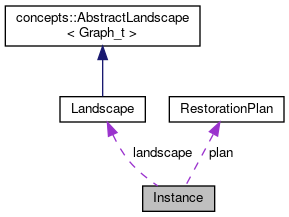
\includegraphics[width=289pt]{class_instance__coll__graph}
\end{center}
\end{figure}
\subsection*{Public Member Functions}
\begin{DoxyCompactItemize}
\item 
\hyperlink{class_instance_a399506c7e75ab9ab78fbc34a25932bbd}{Instance} ()
\end{DoxyCompactItemize}
\subsection*{Public Attributes}
\begin{DoxyCompactItemize}
\item 
\hyperlink{class_landscape}{Landscape} \hyperlink{class_instance_a5a255c00cd67699f9aed6a3402f94560}{landscape}
\item 
const \hyperlink{pl__reff_8cpp_a65aea14f39d53b24df9910d54216d620}{Graph\+\_\+t} \& \hyperlink{class_instance_a7b76d85eaacaec2480ceed2218108013}{graph}
\item 
\hyperlink{class_restoration_plan}{Restoration\+Plan} \hyperlink{class_instance_a95435f6fe84c71114f4e47160854d621}{plan}
\end{DoxyCompactItemize}


\subsection{Constructor \& Destructor Documentation}
\mbox{\Hypertarget{class_instance_a399506c7e75ab9ab78fbc34a25932bbd}\label{class_instance_a399506c7e75ab9ab78fbc34a25932bbd}} 
\index{Instance@{Instance}!Instance@{Instance}}
\index{Instance@{Instance}!Instance@{Instance}}
\subsubsection{\texorpdfstring{Instance()}{Instance()}}
{\footnotesize\ttfamily Instance\+::\+Instance (\begin{DoxyParamCaption}{ }\end{DoxyParamCaption})\hspace{0.3cm}{\ttfamily [inline]}}



\subsection{Member Data Documentation}
\mbox{\Hypertarget{class_instance_a7b76d85eaacaec2480ceed2218108013}\label{class_instance_a7b76d85eaacaec2480ceed2218108013}} 
\index{Instance@{Instance}!graph@{graph}}
\index{graph@{graph}!Instance@{Instance}}
\subsubsection{\texorpdfstring{graph}{graph}}
{\footnotesize\ttfamily const \hyperlink{pl__reff_8cpp_a65aea14f39d53b24df9910d54216d620}{Graph\+\_\+t}\& Instance\+::graph}

\mbox{\Hypertarget{class_instance_a5a255c00cd67699f9aed6a3402f94560}\label{class_instance_a5a255c00cd67699f9aed6a3402f94560}} 
\index{Instance@{Instance}!landscape@{landscape}}
\index{landscape@{landscape}!Instance@{Instance}}
\subsubsection{\texorpdfstring{landscape}{landscape}}
{\footnotesize\ttfamily \hyperlink{class_landscape}{Landscape} Instance\+::landscape}

\mbox{\Hypertarget{class_instance_a95435f6fe84c71114f4e47160854d621}\label{class_instance_a95435f6fe84c71114f4e47160854d621}} 
\index{Instance@{Instance}!plan@{plan}}
\index{plan@{plan}!Instance@{Instance}}
\subsubsection{\texorpdfstring{plan}{plan}}
{\footnotesize\ttfamily \hyperlink{class_restoration_plan}{Restoration\+Plan} Instance\+::plan}



The documentation for this class was generated from the following file\+:\begin{DoxyCompactItemize}
\item 
/home/plaiseek/\+Projects/landscape\+\_\+opt\+\_\+cpp/include/\hyperlink{instances__helper_8hpp}{instances\+\_\+helper.\+hpp}\end{DoxyCompactItemize}

\hypertarget{classconcepts_1_1_solver_1_1_int_param}{}\section{concepts\+:\+:Solver\+:\+:Int\+Param Class Reference}
\label{classconcepts_1_1_solver_1_1_int_param}\index{concepts\+::\+Solver\+::\+Int\+Param@{concepts\+::\+Solver\+::\+Int\+Param}}


{\ttfamily \#include $<$solver.\+hpp$>$}



Inheritance diagram for concepts\+:\+:Solver\+:\+:Int\+Param\+:\nopagebreak
\begin{figure}[H]
\begin{center}
\leavevmode
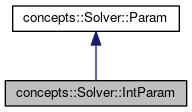
\includegraphics[width=216pt]{classconcepts_1_1_solver_1_1_int_param__inherit__graph}
\end{center}
\end{figure}


Collaboration diagram for concepts\+:\+:Solver\+:\+:Int\+Param\+:\nopagebreak
\begin{figure}[H]
\begin{center}
\leavevmode
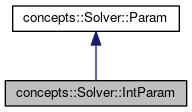
\includegraphics[width=216pt]{classconcepts_1_1_solver_1_1_int_param__coll__graph}
\end{center}
\end{figure}
\subsection*{Public Member Functions}
\begin{DoxyCompactItemize}
\item 
\hyperlink{classconcepts_1_1_solver_1_1_int_param_ae0ca602547edf8a03c323f6bd93e332e}{Int\+Param} (int v)
\item 
void \hyperlink{classconcepts_1_1_solver_1_1_int_param_a81c8c88fe73047c6c1b8d5a87d70be24}{parse} (const char $\ast$arg)
\item 
void \hyperlink{classconcepts_1_1_solver_1_1_int_param_aad1fef920b810b30289a2863d4ab6a52}{set} (bool v)
\item 
void \hyperlink{classconcepts_1_1_solver_1_1_int_param_aad283b6869373847cf9543e889f9fc91}{set} (int v)
\item 
void \hyperlink{classconcepts_1_1_solver_1_1_int_param_aa678f7356cd371ac1bc11e86e0109ae7}{set} (double v)
\item 
bool \hyperlink{classconcepts_1_1_solver_1_1_int_param_aa991108bd194ff4f9cb21230549a74f5}{get\+Bool} () const
\item 
int \hyperlink{classconcepts_1_1_solver_1_1_int_param_a8ff3d45bcc5fc60750183e61ff61b48e}{get\+Int} () const
\item 
double \hyperlink{classconcepts_1_1_solver_1_1_int_param_a70b472a5cce3b44e0d9a08f5da70e1a4}{get\+Double} () const
\item 
std\+::string \hyperlink{classconcepts_1_1_solver_1_1_int_param_a84740f9d96205d4b7fbc1e011a82e08b}{to\+String} () const
\end{DoxyCompactItemize}
\subsection*{Protected Attributes}
\begin{DoxyCompactItemize}
\item 
int \hyperlink{classconcepts_1_1_solver_1_1_int_param_a54714a8509c12174fdd81a92d3ed63d5}{value}
\end{DoxyCompactItemize}


\subsection{Constructor \& Destructor Documentation}
\mbox{\Hypertarget{classconcepts_1_1_solver_1_1_int_param_ae0ca602547edf8a03c323f6bd93e332e}\label{classconcepts_1_1_solver_1_1_int_param_ae0ca602547edf8a03c323f6bd93e332e}} 
\index{concepts\+::\+Solver\+::\+Int\+Param@{concepts\+::\+Solver\+::\+Int\+Param}!Int\+Param@{Int\+Param}}
\index{Int\+Param@{Int\+Param}!concepts\+::\+Solver\+::\+Int\+Param@{concepts\+::\+Solver\+::\+Int\+Param}}
\subsubsection{\texorpdfstring{Int\+Param()}{IntParam()}}
{\footnotesize\ttfamily concepts\+::\+Solver\+::\+Int\+Param\+::\+Int\+Param (\begin{DoxyParamCaption}\item[{int}]{v }\end{DoxyParamCaption})\hspace{0.3cm}{\ttfamily [inline]}}



\subsection{Member Function Documentation}
\mbox{\Hypertarget{classconcepts_1_1_solver_1_1_int_param_aa991108bd194ff4f9cb21230549a74f5}\label{classconcepts_1_1_solver_1_1_int_param_aa991108bd194ff4f9cb21230549a74f5}} 
\index{concepts\+::\+Solver\+::\+Int\+Param@{concepts\+::\+Solver\+::\+Int\+Param}!get\+Bool@{get\+Bool}}
\index{get\+Bool@{get\+Bool}!concepts\+::\+Solver\+::\+Int\+Param@{concepts\+::\+Solver\+::\+Int\+Param}}
\subsubsection{\texorpdfstring{get\+Bool()}{getBool()}}
{\footnotesize\ttfamily bool concepts\+::\+Solver\+::\+Int\+Param\+::get\+Bool (\begin{DoxyParamCaption}{ }\end{DoxyParamCaption}) const\hspace{0.3cm}{\ttfamily [inline]}, {\ttfamily [virtual]}}



Implements \hyperlink{classconcepts_1_1_solver_1_1_param_aaca8a78f4669d189764e9e654143d705}{concepts\+::\+Solver\+::\+Param}.

\mbox{\Hypertarget{classconcepts_1_1_solver_1_1_int_param_a70b472a5cce3b44e0d9a08f5da70e1a4}\label{classconcepts_1_1_solver_1_1_int_param_a70b472a5cce3b44e0d9a08f5da70e1a4}} 
\index{concepts\+::\+Solver\+::\+Int\+Param@{concepts\+::\+Solver\+::\+Int\+Param}!get\+Double@{get\+Double}}
\index{get\+Double@{get\+Double}!concepts\+::\+Solver\+::\+Int\+Param@{concepts\+::\+Solver\+::\+Int\+Param}}
\subsubsection{\texorpdfstring{get\+Double()}{getDouble()}}
{\footnotesize\ttfamily double concepts\+::\+Solver\+::\+Int\+Param\+::get\+Double (\begin{DoxyParamCaption}{ }\end{DoxyParamCaption}) const\hspace{0.3cm}{\ttfamily [inline]}, {\ttfamily [virtual]}}



Implements \hyperlink{classconcepts_1_1_solver_1_1_param_a50d288b81da0b77d342e46e75f9b4bfc}{concepts\+::\+Solver\+::\+Param}.

\mbox{\Hypertarget{classconcepts_1_1_solver_1_1_int_param_a8ff3d45bcc5fc60750183e61ff61b48e}\label{classconcepts_1_1_solver_1_1_int_param_a8ff3d45bcc5fc60750183e61ff61b48e}} 
\index{concepts\+::\+Solver\+::\+Int\+Param@{concepts\+::\+Solver\+::\+Int\+Param}!get\+Int@{get\+Int}}
\index{get\+Int@{get\+Int}!concepts\+::\+Solver\+::\+Int\+Param@{concepts\+::\+Solver\+::\+Int\+Param}}
\subsubsection{\texorpdfstring{get\+Int()}{getInt()}}
{\footnotesize\ttfamily int concepts\+::\+Solver\+::\+Int\+Param\+::get\+Int (\begin{DoxyParamCaption}{ }\end{DoxyParamCaption}) const\hspace{0.3cm}{\ttfamily [inline]}, {\ttfamily [virtual]}}



Implements \hyperlink{classconcepts_1_1_solver_1_1_param_ab849633a029055c00d828df3adb0546e}{concepts\+::\+Solver\+::\+Param}.

\mbox{\Hypertarget{classconcepts_1_1_solver_1_1_int_param_a81c8c88fe73047c6c1b8d5a87d70be24}\label{classconcepts_1_1_solver_1_1_int_param_a81c8c88fe73047c6c1b8d5a87d70be24}} 
\index{concepts\+::\+Solver\+::\+Int\+Param@{concepts\+::\+Solver\+::\+Int\+Param}!parse@{parse}}
\index{parse@{parse}!concepts\+::\+Solver\+::\+Int\+Param@{concepts\+::\+Solver\+::\+Int\+Param}}
\subsubsection{\texorpdfstring{parse()}{parse()}}
{\footnotesize\ttfamily void concepts\+::\+Solver\+::\+Int\+Param\+::parse (\begin{DoxyParamCaption}\item[{const char $\ast$}]{arg }\end{DoxyParamCaption})\hspace{0.3cm}{\ttfamily [inline]}, {\ttfamily [virtual]}}



Implements \hyperlink{classconcepts_1_1_solver_1_1_param_a0c2e4d895747668b01339db9226eceae}{concepts\+::\+Solver\+::\+Param}.

\mbox{\Hypertarget{classconcepts_1_1_solver_1_1_int_param_aad1fef920b810b30289a2863d4ab6a52}\label{classconcepts_1_1_solver_1_1_int_param_aad1fef920b810b30289a2863d4ab6a52}} 
\index{concepts\+::\+Solver\+::\+Int\+Param@{concepts\+::\+Solver\+::\+Int\+Param}!set@{set}}
\index{set@{set}!concepts\+::\+Solver\+::\+Int\+Param@{concepts\+::\+Solver\+::\+Int\+Param}}
\subsubsection{\texorpdfstring{set()}{set()}\hspace{0.1cm}{\footnotesize\ttfamily [1/3]}}
{\footnotesize\ttfamily void concepts\+::\+Solver\+::\+Int\+Param\+::set (\begin{DoxyParamCaption}\item[{bool}]{v }\end{DoxyParamCaption})\hspace{0.3cm}{\ttfamily [inline]}, {\ttfamily [virtual]}}



Implements \hyperlink{classconcepts_1_1_solver_1_1_param_aa525a1a88dd771eaf5d66f35323fbb86}{concepts\+::\+Solver\+::\+Param}.

\mbox{\Hypertarget{classconcepts_1_1_solver_1_1_int_param_aad283b6869373847cf9543e889f9fc91}\label{classconcepts_1_1_solver_1_1_int_param_aad283b6869373847cf9543e889f9fc91}} 
\index{concepts\+::\+Solver\+::\+Int\+Param@{concepts\+::\+Solver\+::\+Int\+Param}!set@{set}}
\index{set@{set}!concepts\+::\+Solver\+::\+Int\+Param@{concepts\+::\+Solver\+::\+Int\+Param}}
\subsubsection{\texorpdfstring{set()}{set()}\hspace{0.1cm}{\footnotesize\ttfamily [2/3]}}
{\footnotesize\ttfamily void concepts\+::\+Solver\+::\+Int\+Param\+::set (\begin{DoxyParamCaption}\item[{int}]{v }\end{DoxyParamCaption})\hspace{0.3cm}{\ttfamily [inline]}, {\ttfamily [virtual]}}



Implements \hyperlink{classconcepts_1_1_solver_1_1_param_ad3de8144a70e67eeae4278f534e46274}{concepts\+::\+Solver\+::\+Param}.

\mbox{\Hypertarget{classconcepts_1_1_solver_1_1_int_param_aa678f7356cd371ac1bc11e86e0109ae7}\label{classconcepts_1_1_solver_1_1_int_param_aa678f7356cd371ac1bc11e86e0109ae7}} 
\index{concepts\+::\+Solver\+::\+Int\+Param@{concepts\+::\+Solver\+::\+Int\+Param}!set@{set}}
\index{set@{set}!concepts\+::\+Solver\+::\+Int\+Param@{concepts\+::\+Solver\+::\+Int\+Param}}
\subsubsection{\texorpdfstring{set()}{set()}\hspace{0.1cm}{\footnotesize\ttfamily [3/3]}}
{\footnotesize\ttfamily void concepts\+::\+Solver\+::\+Int\+Param\+::set (\begin{DoxyParamCaption}\item[{double}]{v }\end{DoxyParamCaption})\hspace{0.3cm}{\ttfamily [inline]}, {\ttfamily [virtual]}}



Implements \hyperlink{classconcepts_1_1_solver_1_1_param_a35b7155d8f6db1b3e63e60b883beebcb}{concepts\+::\+Solver\+::\+Param}.

\mbox{\Hypertarget{classconcepts_1_1_solver_1_1_int_param_a84740f9d96205d4b7fbc1e011a82e08b}\label{classconcepts_1_1_solver_1_1_int_param_a84740f9d96205d4b7fbc1e011a82e08b}} 
\index{concepts\+::\+Solver\+::\+Int\+Param@{concepts\+::\+Solver\+::\+Int\+Param}!to\+String@{to\+String}}
\index{to\+String@{to\+String}!concepts\+::\+Solver\+::\+Int\+Param@{concepts\+::\+Solver\+::\+Int\+Param}}
\subsubsection{\texorpdfstring{to\+String()}{toString()}}
{\footnotesize\ttfamily std\+::string concepts\+::\+Solver\+::\+Int\+Param\+::to\+String (\begin{DoxyParamCaption}{ }\end{DoxyParamCaption}) const\hspace{0.3cm}{\ttfamily [inline]}, {\ttfamily [virtual]}}



Implements \hyperlink{classconcepts_1_1_solver_1_1_param_abcbd9c68852499c7be9ebf6a2d22f4b5}{concepts\+::\+Solver\+::\+Param}.



\subsection{Member Data Documentation}
\mbox{\Hypertarget{classconcepts_1_1_solver_1_1_int_param_a54714a8509c12174fdd81a92d3ed63d5}\label{classconcepts_1_1_solver_1_1_int_param_a54714a8509c12174fdd81a92d3ed63d5}} 
\index{concepts\+::\+Solver\+::\+Int\+Param@{concepts\+::\+Solver\+::\+Int\+Param}!value@{value}}
\index{value@{value}!concepts\+::\+Solver\+::\+Int\+Param@{concepts\+::\+Solver\+::\+Int\+Param}}
\subsubsection{\texorpdfstring{value}{value}}
{\footnotesize\ttfamily int concepts\+::\+Solver\+::\+Int\+Param\+::value\hspace{0.3cm}{\ttfamily [protected]}}



The documentation for this class was generated from the following file\+:\begin{DoxyCompactItemize}
\item 
/home/plaiseek/\+Projects/landscape\+\_\+opt\+\_\+cpp/include/solvers/concept/\hyperlink{solver_8hpp}{solver.\+hpp}\end{DoxyCompactItemize}

\hypertarget{classlemon_1_1_labeled_value}{}\section{lemon\+:\+:Labeled\+Value$<$ V $>$ Class Template Reference}
\label{classlemon_1_1_labeled_value}\index{lemon\+::\+Labeled\+Value$<$ V $>$@{lemon\+::\+Labeled\+Value$<$ V $>$}}


{\ttfamily \#include $<$identify\+\_\+strong\+\_\+arcs.\+h$>$}

\subsection*{Public Member Functions}
\begin{DoxyCompactItemize}
\item 
\hyperlink{classlemon_1_1_labeled_value_a14eecff046442f7d6ddca93014e95b05}{Labeled\+Value} ()
\item 
\hyperlink{classlemon_1_1_labeled_value_a95f29b1d3308d805fa51a13790cd08f0}{Labeled\+Value} (const Value \&\hyperlink{classlemon_1_1_labeled_value_ad52008450e02d6f966a512f45cccd695}{value}, bool \hyperlink{classlemon_1_1_labeled_value_a2e6cbc625abb719205f698a1ee605f34}{label}=false)
\item 
\hyperlink{classlemon_1_1_labeled_value_a92e5bba9725478c716bf918a98821ebf}{Labeled\+Value} (const \hyperlink{classlemon_1_1_labeled_value}{Labeled\+Value}$<$ Value $>$ \&o)
\item 
bool \hyperlink{classlemon_1_1_labeled_value_ac391a3b4e250a3484f215c1ef3649a28}{operator$<$} (const \hyperlink{classlemon_1_1_labeled_value}{Labeled\+Value}$<$ Value $>$ \&o) const
\item 
bool \hyperlink{classlemon_1_1_labeled_value_afecbbe1dee2fa63f3c8eecbf258e6b81}{operator$>$} (const \hyperlink{classlemon_1_1_labeled_value}{Labeled\+Value}$<$ Value $>$ \&o) const
\item 
bool \hyperlink{classlemon_1_1_labeled_value_a67101fc1931e05d142d79cb0d5c00db3}{operator==} (const \hyperlink{classlemon_1_1_labeled_value}{Labeled\+Value}$<$ Value $>$ \&o) const
\item 
void \hyperlink{classlemon_1_1_labeled_value_adb93ba08026dd33dfb2c4160adf2a81c}{operator=} (const \hyperlink{classlemon_1_1_labeled_value}{Labeled\+Value}$<$ Value $>$ \&o)
\item 
void \hyperlink{classlemon_1_1_labeled_value_aab6fe896646c831d1b6fa4f030b325b2}{operator=} (const Value \&o)
\item 
\hyperlink{classlemon_1_1_labeled_value}{Labeled\+Value}$<$ Value $>$ \hyperlink{classlemon_1_1_labeled_value_a16e6e3856d8afec132b0527dd93dfce5}{operator+} (const \hyperlink{classlemon_1_1_labeled_value}{Labeled\+Value}$<$ Value $>$ \&o) const
\item 
\hyperlink{classlemon_1_1_labeled_value}{Labeled\+Value}$<$ Value $>$ \hyperlink{classlemon_1_1_labeled_value_aaf3a95a408db36775ef7298d9b10f5e5}{operator$\ast$} (const \hyperlink{classlemon_1_1_labeled_value}{Labeled\+Value}$<$ Value $>$ \&o) const
\end{DoxyCompactItemize}
\subsection*{Public Attributes}
\begin{DoxyCompactItemize}
\item 
Value \hyperlink{classlemon_1_1_labeled_value_ad52008450e02d6f966a512f45cccd695}{value}
\item 
bool \hyperlink{classlemon_1_1_labeled_value_a2e6cbc625abb719205f698a1ee605f34}{label}
\end{DoxyCompactItemize}


\subsection{Constructor \& Destructor Documentation}
\mbox{\Hypertarget{classlemon_1_1_labeled_value_a14eecff046442f7d6ddca93014e95b05}\label{classlemon_1_1_labeled_value_a14eecff046442f7d6ddca93014e95b05}} 
\index{lemon\+::\+Labeled\+Value@{lemon\+::\+Labeled\+Value}!Labeled\+Value@{Labeled\+Value}}
\index{Labeled\+Value@{Labeled\+Value}!lemon\+::\+Labeled\+Value@{lemon\+::\+Labeled\+Value}}
\subsubsection{\texorpdfstring{Labeled\+Value()}{LabeledValue()}\hspace{0.1cm}{\footnotesize\ttfamily [1/3]}}
{\footnotesize\ttfamily template$<$typename V$>$ \\
\hyperlink{classlemon_1_1_labeled_value}{lemon\+::\+Labeled\+Value}$<$ V $>$\+::\hyperlink{classlemon_1_1_labeled_value}{Labeled\+Value} (\begin{DoxyParamCaption}{ }\end{DoxyParamCaption})\hspace{0.3cm}{\ttfamily [inline]}}

\mbox{\Hypertarget{classlemon_1_1_labeled_value_a95f29b1d3308d805fa51a13790cd08f0}\label{classlemon_1_1_labeled_value_a95f29b1d3308d805fa51a13790cd08f0}} 
\index{lemon\+::\+Labeled\+Value@{lemon\+::\+Labeled\+Value}!Labeled\+Value@{Labeled\+Value}}
\index{Labeled\+Value@{Labeled\+Value}!lemon\+::\+Labeled\+Value@{lemon\+::\+Labeled\+Value}}
\subsubsection{\texorpdfstring{Labeled\+Value()}{LabeledValue()}\hspace{0.1cm}{\footnotesize\ttfamily [2/3]}}
{\footnotesize\ttfamily template$<$typename V$>$ \\
\hyperlink{classlemon_1_1_labeled_value}{lemon\+::\+Labeled\+Value}$<$ V $>$\+::\hyperlink{classlemon_1_1_labeled_value}{Labeled\+Value} (\begin{DoxyParamCaption}\item[{const Value \&}]{value,  }\item[{bool}]{label = {\ttfamily false} }\end{DoxyParamCaption})\hspace{0.3cm}{\ttfamily [inline]}}

\mbox{\Hypertarget{classlemon_1_1_labeled_value_a92e5bba9725478c716bf918a98821ebf}\label{classlemon_1_1_labeled_value_a92e5bba9725478c716bf918a98821ebf}} 
\index{lemon\+::\+Labeled\+Value@{lemon\+::\+Labeled\+Value}!Labeled\+Value@{Labeled\+Value}}
\index{Labeled\+Value@{Labeled\+Value}!lemon\+::\+Labeled\+Value@{lemon\+::\+Labeled\+Value}}
\subsubsection{\texorpdfstring{Labeled\+Value()}{LabeledValue()}\hspace{0.1cm}{\footnotesize\ttfamily [3/3]}}
{\footnotesize\ttfamily template$<$typename V$>$ \\
\hyperlink{classlemon_1_1_labeled_value}{lemon\+::\+Labeled\+Value}$<$ V $>$\+::\hyperlink{classlemon_1_1_labeled_value}{Labeled\+Value} (\begin{DoxyParamCaption}\item[{const \hyperlink{classlemon_1_1_labeled_value}{Labeled\+Value}$<$ Value $>$ \&}]{o }\end{DoxyParamCaption})\hspace{0.3cm}{\ttfamily [inline]}}



\subsection{Member Function Documentation}
\mbox{\Hypertarget{classlemon_1_1_labeled_value_aaf3a95a408db36775ef7298d9b10f5e5}\label{classlemon_1_1_labeled_value_aaf3a95a408db36775ef7298d9b10f5e5}} 
\index{lemon\+::\+Labeled\+Value@{lemon\+::\+Labeled\+Value}!operator$\ast$@{operator$\ast$}}
\index{operator$\ast$@{operator$\ast$}!lemon\+::\+Labeled\+Value@{lemon\+::\+Labeled\+Value}}
\subsubsection{\texorpdfstring{operator$\ast$()}{operator*()}}
{\footnotesize\ttfamily template$<$typename V$>$ \\
\hyperlink{classlemon_1_1_labeled_value}{Labeled\+Value}$<$Value$>$ \hyperlink{classlemon_1_1_labeled_value}{lemon\+::\+Labeled\+Value}$<$ V $>$\+::operator$\ast$ (\begin{DoxyParamCaption}\item[{const \hyperlink{classlemon_1_1_labeled_value}{Labeled\+Value}$<$ Value $>$ \&}]{o }\end{DoxyParamCaption}) const\hspace{0.3cm}{\ttfamily [inline]}}

\mbox{\Hypertarget{classlemon_1_1_labeled_value_a16e6e3856d8afec132b0527dd93dfce5}\label{classlemon_1_1_labeled_value_a16e6e3856d8afec132b0527dd93dfce5}} 
\index{lemon\+::\+Labeled\+Value@{lemon\+::\+Labeled\+Value}!operator+@{operator+}}
\index{operator+@{operator+}!lemon\+::\+Labeled\+Value@{lemon\+::\+Labeled\+Value}}
\subsubsection{\texorpdfstring{operator+()}{operator+()}}
{\footnotesize\ttfamily template$<$typename V$>$ \\
\hyperlink{classlemon_1_1_labeled_value}{Labeled\+Value}$<$Value$>$ \hyperlink{classlemon_1_1_labeled_value}{lemon\+::\+Labeled\+Value}$<$ V $>$\+::operator+ (\begin{DoxyParamCaption}\item[{const \hyperlink{classlemon_1_1_labeled_value}{Labeled\+Value}$<$ Value $>$ \&}]{o }\end{DoxyParamCaption}) const\hspace{0.3cm}{\ttfamily [inline]}}

\mbox{\Hypertarget{classlemon_1_1_labeled_value_ac391a3b4e250a3484f215c1ef3649a28}\label{classlemon_1_1_labeled_value_ac391a3b4e250a3484f215c1ef3649a28}} 
\index{lemon\+::\+Labeled\+Value@{lemon\+::\+Labeled\+Value}!operator$<$@{operator$<$}}
\index{operator$<$@{operator$<$}!lemon\+::\+Labeled\+Value@{lemon\+::\+Labeled\+Value}}
\subsubsection{\texorpdfstring{operator$<$()}{operator<()}}
{\footnotesize\ttfamily template$<$typename V$>$ \\
bool \hyperlink{classlemon_1_1_labeled_value}{lemon\+::\+Labeled\+Value}$<$ V $>$\+::operator$<$ (\begin{DoxyParamCaption}\item[{const \hyperlink{classlemon_1_1_labeled_value}{Labeled\+Value}$<$ Value $>$ \&}]{o }\end{DoxyParamCaption}) const\hspace{0.3cm}{\ttfamily [inline]}}

\mbox{\Hypertarget{classlemon_1_1_labeled_value_adb93ba08026dd33dfb2c4160adf2a81c}\label{classlemon_1_1_labeled_value_adb93ba08026dd33dfb2c4160adf2a81c}} 
\index{lemon\+::\+Labeled\+Value@{lemon\+::\+Labeled\+Value}!operator=@{operator=}}
\index{operator=@{operator=}!lemon\+::\+Labeled\+Value@{lemon\+::\+Labeled\+Value}}
\subsubsection{\texorpdfstring{operator=()}{operator=()}\hspace{0.1cm}{\footnotesize\ttfamily [1/2]}}
{\footnotesize\ttfamily template$<$typename V$>$ \\
void \hyperlink{classlemon_1_1_labeled_value}{lemon\+::\+Labeled\+Value}$<$ V $>$\+::operator= (\begin{DoxyParamCaption}\item[{const \hyperlink{classlemon_1_1_labeled_value}{Labeled\+Value}$<$ Value $>$ \&}]{o }\end{DoxyParamCaption})\hspace{0.3cm}{\ttfamily [inline]}}

\mbox{\Hypertarget{classlemon_1_1_labeled_value_aab6fe896646c831d1b6fa4f030b325b2}\label{classlemon_1_1_labeled_value_aab6fe896646c831d1b6fa4f030b325b2}} 
\index{lemon\+::\+Labeled\+Value@{lemon\+::\+Labeled\+Value}!operator=@{operator=}}
\index{operator=@{operator=}!lemon\+::\+Labeled\+Value@{lemon\+::\+Labeled\+Value}}
\subsubsection{\texorpdfstring{operator=()}{operator=()}\hspace{0.1cm}{\footnotesize\ttfamily [2/2]}}
{\footnotesize\ttfamily template$<$typename V$>$ \\
void \hyperlink{classlemon_1_1_labeled_value}{lemon\+::\+Labeled\+Value}$<$ V $>$\+::operator= (\begin{DoxyParamCaption}\item[{const Value \&}]{o }\end{DoxyParamCaption})\hspace{0.3cm}{\ttfamily [inline]}}

\mbox{\Hypertarget{classlemon_1_1_labeled_value_a67101fc1931e05d142d79cb0d5c00db3}\label{classlemon_1_1_labeled_value_a67101fc1931e05d142d79cb0d5c00db3}} 
\index{lemon\+::\+Labeled\+Value@{lemon\+::\+Labeled\+Value}!operator==@{operator==}}
\index{operator==@{operator==}!lemon\+::\+Labeled\+Value@{lemon\+::\+Labeled\+Value}}
\subsubsection{\texorpdfstring{operator==()}{operator==()}}
{\footnotesize\ttfamily template$<$typename V$>$ \\
bool \hyperlink{classlemon_1_1_labeled_value}{lemon\+::\+Labeled\+Value}$<$ V $>$\+::operator== (\begin{DoxyParamCaption}\item[{const \hyperlink{classlemon_1_1_labeled_value}{Labeled\+Value}$<$ Value $>$ \&}]{o }\end{DoxyParamCaption}) const\hspace{0.3cm}{\ttfamily [inline]}}

\mbox{\Hypertarget{classlemon_1_1_labeled_value_afecbbe1dee2fa63f3c8eecbf258e6b81}\label{classlemon_1_1_labeled_value_afecbbe1dee2fa63f3c8eecbf258e6b81}} 
\index{lemon\+::\+Labeled\+Value@{lemon\+::\+Labeled\+Value}!operator$>$@{operator$>$}}
\index{operator$>$@{operator$>$}!lemon\+::\+Labeled\+Value@{lemon\+::\+Labeled\+Value}}
\subsubsection{\texorpdfstring{operator$>$()}{operator>()}}
{\footnotesize\ttfamily template$<$typename V$>$ \\
bool \hyperlink{classlemon_1_1_labeled_value}{lemon\+::\+Labeled\+Value}$<$ V $>$\+::operator$>$ (\begin{DoxyParamCaption}\item[{const \hyperlink{classlemon_1_1_labeled_value}{Labeled\+Value}$<$ Value $>$ \&}]{o }\end{DoxyParamCaption}) const\hspace{0.3cm}{\ttfamily [inline]}}



\subsection{Member Data Documentation}
\mbox{\Hypertarget{classlemon_1_1_labeled_value_a2e6cbc625abb719205f698a1ee605f34}\label{classlemon_1_1_labeled_value_a2e6cbc625abb719205f698a1ee605f34}} 
\index{lemon\+::\+Labeled\+Value@{lemon\+::\+Labeled\+Value}!label@{label}}
\index{label@{label}!lemon\+::\+Labeled\+Value@{lemon\+::\+Labeled\+Value}}
\subsubsection{\texorpdfstring{label}{label}}
{\footnotesize\ttfamily template$<$typename V$>$ \\
bool \hyperlink{classlemon_1_1_labeled_value}{lemon\+::\+Labeled\+Value}$<$ V $>$\+::label}

\mbox{\Hypertarget{classlemon_1_1_labeled_value_ad52008450e02d6f966a512f45cccd695}\label{classlemon_1_1_labeled_value_ad52008450e02d6f966a512f45cccd695}} 
\index{lemon\+::\+Labeled\+Value@{lemon\+::\+Labeled\+Value}!value@{value}}
\index{value@{value}!lemon\+::\+Labeled\+Value@{lemon\+::\+Labeled\+Value}}
\subsubsection{\texorpdfstring{value}{value}}
{\footnotesize\ttfamily template$<$typename V$>$ \\
Value \hyperlink{classlemon_1_1_labeled_value}{lemon\+::\+Labeled\+Value}$<$ V $>$\+::value}



The documentation for this class was generated from the following file\+:\begin{DoxyCompactItemize}
\item 
/home/plaiseek/\+Projects/landscape\+\_\+opt\+\_\+cpp/include/algorithms/\hyperlink{identify__strong__arcs_8h}{identify\+\_\+strong\+\_\+arcs.\+h}\end{DoxyCompactItemize}

\hypertarget{class_landscape}{}\section{Landscape Class Reference}
\label{class_landscape}\index{Landscape@{Landscape}}


Class that represent an editable landscape.  




{\ttfamily \#include $<$landscape.\+hpp$>$}



Inheritance diagram for Landscape\+:\nopagebreak
\begin{figure}[H]
\begin{center}
\leavevmode
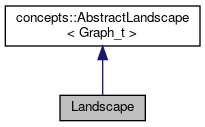
\includegraphics[width=226pt]{class_landscape__inherit__graph}
\end{center}
\end{figure}


Collaboration diagram for Landscape\+:\nopagebreak
\begin{figure}[H]
\begin{center}
\leavevmode
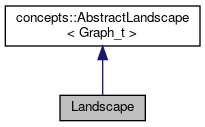
\includegraphics[width=226pt]{class_landscape__coll__graph}
\end{center}
\end{figure}
\subsection*{Public Member Functions}
\begin{DoxyCompactItemize}
\item 
\hyperlink{class_landscape_a0a54d8aabc38c0a5aa27ccace3f91915}{Landscape} ()
\item 
\hyperlink{class_landscape_a44c62eb1b0f84a40f25b9a6445c8b130}{$\sim$\+Landscape} ()
\item 
std\+::pair$<$ Graph\+\_\+t\+::\+Node\+Map$<$ \hyperlink{classconcepts_1_1_abstract_landscape_a7c2f90fb9f42302f1af84a59f4df4b91}{Node} $>$ $\ast$, Graph\+\_\+t\+::\+Arc\+Map$<$ \hyperlink{classconcepts_1_1_abstract_landscape_a0966623f028fe50ac9a3ae114dcf2672}{Arc} $>$ $\ast$ $>$ \hyperlink{class_landscape_a72ac309bcc23cf55888967b4da22ad6f}{copy} (const \hyperlink{class_landscape}{Landscape} \&orig\+\_\+landscape)
\begin{DoxyCompactList}\small\item\em Makes the current landscape a copy of the one passed in parameter. \end{DoxyCompactList}\item 
\hyperlink{classconcepts_1_1_abstract_landscape_a7c2f90fb9f42302f1af84a59f4df4b91}{Node} \hyperlink{class_landscape_a7fbed383ff33eee7dad4be3794a5c38b}{add\+Node} (double quality, \hyperlink{abstract__landscape_8hpp_a9c14bcba65b035519a9c98f1eb1babbe}{Point} coords)
\begin{DoxyCompactList}\small\item\em Adds a new patch with specified quality and coordinates. \end{DoxyCompactList}\item 
\hyperlink{classconcepts_1_1_abstract_landscape_a0966623f028fe50ac9a3ae114dcf2672}{Arc} \hyperlink{class_landscape_a838233aa09155408cd938405aa504289}{add\+Arc} (\hyperlink{classconcepts_1_1_abstract_landscape_a7c2f90fb9f42302f1af84a59f4df4b91}{Node} u, \hyperlink{classconcepts_1_1_abstract_landscape_a7c2f90fb9f42302f1af84a59f4df4b91}{Node} v, double difficulty)
\begin{DoxyCompactList}\small\item\em Adds a new arc from u to v with specified probability. \end{DoxyCompactList}\item 
void \hyperlink{class_landscape_a800ffffd591570d5a19a030707f51365}{remove\+Node} (\hyperlink{classconcepts_1_1_abstract_landscape_a7c2f90fb9f42302f1af84a59f4df4b91}{Node} u)
\begin{DoxyCompactList}\small\item\em Removes the node u. \end{DoxyCompactList}\item 
void \hyperlink{class_landscape_ada96d1d07c462e043133440f647211b2}{remove\+Arc} (\hyperlink{classconcepts_1_1_abstract_landscape_a0966623f028fe50ac9a3ae114dcf2672}{Arc} a)
\begin{DoxyCompactList}\small\item\em Removes the arc a. \end{DoxyCompactList}\item 
void \hyperlink{class_landscape_ae176491eae8fec5777ab8566cc8bf64f}{change\+Source} (\hyperlink{classconcepts_1_1_abstract_landscape_a0966623f028fe50ac9a3ae114dcf2672}{Arc} a, \hyperlink{classconcepts_1_1_abstract_landscape_a7c2f90fb9f42302f1af84a59f4df4b91}{Node} u)
\begin{DoxyCompactList}\small\item\em Changes the source of the arc a to be u. \end{DoxyCompactList}\item 
void \hyperlink{class_landscape_a4bbe12577926a357f715d8e91c393ec4}{change\+Target} (\hyperlink{classconcepts_1_1_abstract_landscape_a0966623f028fe50ac9a3ae114dcf2672}{Arc} a, \hyperlink{classconcepts_1_1_abstract_landscape_a7c2f90fb9f42302f1af84a59f4df4b91}{Node} v)
\begin{DoxyCompactList}\small\item\em Changes the source of the arc a to be v. \end{DoxyCompactList}\item 
void \hyperlink{class_landscape_aac673fb693ff152251109c07f60f3672}{set\+Quality} (\hyperlink{classconcepts_1_1_abstract_landscape_a7c2f90fb9f42302f1af84a59f4df4b91}{Node} u, double quality)
\begin{DoxyCompactList}\small\item\em Set the quality of the node u. \end{DoxyCompactList}\item 
void \hyperlink{class_landscape_a4c8df159a4754013dd381bfff23d133d}{set\+Coords} (\hyperlink{classconcepts_1_1_abstract_landscape_a7c2f90fb9f42302f1af84a59f4df4b91}{Node} u, \hyperlink{abstract__landscape_8hpp_a9c14bcba65b035519a9c98f1eb1babbe}{Point} coords)
\begin{DoxyCompactList}\small\item\em Set the coordinates of the node u. \end{DoxyCompactList}\item 
void \hyperlink{class_landscape_abf8fb4b7e4185c9f876aa3afc39d1331}{set\+Probability} (\hyperlink{classconcepts_1_1_abstract_landscape_a0966623f028fe50ac9a3ae114dcf2672}{Arc} a, double probability)
\begin{DoxyCompactList}\small\item\em Set the probability of the arc a. \end{DoxyCompactList}\item 
const \hyperlink{classconcepts_1_1_abstract_landscape_ab1988ca4ff36329c45af21e76046903d}{Graph} \& \hyperlink{class_landscape_a5f372f74530914d9128a036bbdaf7800}{get\+Network} () const
\item 
const \hyperlink{classconcepts_1_1_abstract_landscape_aab540b896ac9b7a7a5783f2a78f304ad}{Quality\+Map} \& \hyperlink{class_landscape_a77f947fdc6a8c8875d7d383eb5ce7817}{get\+Quality\+Map} () const
\item 
const \hyperlink{classconcepts_1_1_abstract_landscape_a8432d7dff7edc5a5cbc524592b411f8a}{Coords\+Map} \& \hyperlink{class_landscape_ab6e4efb27be3f1870ce42656a5534d68}{get\+Coords\+Map} () const
\item 
const \hyperlink{classconcepts_1_1_abstract_landscape_ae90ffb759facff21b29e646539352182}{Probability\+Map} \& \hyperlink{class_landscape_a771053b32bbcb6a3fa5204b8bdb53a6d}{get\+Probability\+Map} () const
\item 
const double \& \hyperlink{class_landscape_a15c6c9bf708e4ceb3a9118157f99659a}{get\+Quality} (\hyperlink{classconcepts_1_1_abstract_landscape_a7c2f90fb9f42302f1af84a59f4df4b91}{Node} u) const
\item 
const \hyperlink{abstract__landscape_8hpp_a9c14bcba65b035519a9c98f1eb1babbe}{Point} \& \hyperlink{class_landscape_a99f206e722c06b938fe1f2e105de310d}{get\+Coords} (\hyperlink{classconcepts_1_1_abstract_landscape_a7c2f90fb9f42302f1af84a59f4df4b91}{Node} u) const
\item 
const double \& \hyperlink{class_landscape_ac251ee7350a51502a1006333894082c3}{get\+Probability} (\hyperlink{classconcepts_1_1_abstract_landscape_a0966623f028fe50ac9a3ae114dcf2672}{Arc} a) const
\item 
double \& \hyperlink{class_landscape_af6fdabb5a81dc4cf75d7baaf6d98ee31}{get\+Quality\+Ref} (\hyperlink{classconcepts_1_1_abstract_landscape_a7c2f90fb9f42302f1af84a59f4df4b91}{Node} u)
\item 
\hyperlink{abstract__landscape_8hpp_a9c14bcba65b035519a9c98f1eb1babbe}{Point} \& \hyperlink{class_landscape_a5c7fb81e36d91b0300815962e1677d5e}{get\+Coords\+Ref} (\hyperlink{classconcepts_1_1_abstract_landscape_a7c2f90fb9f42302f1af84a59f4df4b91}{Node} u)
\item 
double \& \hyperlink{class_landscape_a1d8000badf88704d19ce276743e67a25}{get\+Probability\+Ref} (\hyperlink{classconcepts_1_1_abstract_landscape_a0966623f028fe50ac9a3ae114dcf2672}{Arc} a)
\end{DoxyCompactItemize}
\subsection*{Additional Inherited Members}


\subsection{Detailed Description}
Class that represent an editable landscape. 

This class represent an editable landscape. That is a graph whose nodes weigths are quality and coordinates, and arcs weigths are probabilities to success crossing. 

\subsection{Constructor \& Destructor Documentation}
\mbox{\Hypertarget{class_landscape_a0a54d8aabc38c0a5aa27ccace3f91915}\label{class_landscape_a0a54d8aabc38c0a5aa27ccace3f91915}} 
\index{Landscape@{Landscape}!Landscape@{Landscape}}
\index{Landscape@{Landscape}!Landscape@{Landscape}}
\subsubsection{\texorpdfstring{Landscape()}{Landscape()}}
{\footnotesize\ttfamily Landscape\+::\+Landscape (\begin{DoxyParamCaption}{ }\end{DoxyParamCaption})}

\mbox{\Hypertarget{class_landscape_a44c62eb1b0f84a40f25b9a6445c8b130}\label{class_landscape_a44c62eb1b0f84a40f25b9a6445c8b130}} 
\index{Landscape@{Landscape}!````~Landscape@{$\sim$\+Landscape}}
\index{````~Landscape@{$\sim$\+Landscape}!Landscape@{Landscape}}
\subsubsection{\texorpdfstring{$\sim$\+Landscape()}{~Landscape()}}
{\footnotesize\ttfamily Landscape\+::$\sim$\+Landscape (\begin{DoxyParamCaption}{ }\end{DoxyParamCaption})}



\subsection{Member Function Documentation}
\mbox{\Hypertarget{class_landscape_a838233aa09155408cd938405aa504289}\label{class_landscape_a838233aa09155408cd938405aa504289}} 
\index{Landscape@{Landscape}!add\+Arc@{add\+Arc}}
\index{add\+Arc@{add\+Arc}!Landscape@{Landscape}}
\subsubsection{\texorpdfstring{add\+Arc()}{addArc()}}
{\footnotesize\ttfamily \hyperlink{classconcepts_1_1_abstract_landscape_a0966623f028fe50ac9a3ae114dcf2672}{Landscape\+::\+Arc} Landscape\+::add\+Arc (\begin{DoxyParamCaption}\item[{\hyperlink{classconcepts_1_1_abstract_landscape_a7c2f90fb9f42302f1af84a59f4df4b91}{Node}}]{u,  }\item[{\hyperlink{classconcepts_1_1_abstract_landscape_a7c2f90fb9f42302f1af84a59f4df4b91}{Node}}]{v,  }\item[{double}]{difficulty }\end{DoxyParamCaption})}



Adds a new arc from u to v with specified probability. 


\begin{DoxyParams}{Parameters}
{\em u} & \\
\hline
{\em v} & \\
\hline
{\em difficulty} & \\
\hline
\end{DoxyParams}
\begin{DoxyReturn}{Returns}
the created graph Arc 
\end{DoxyReturn}
\mbox{\Hypertarget{class_landscape_a7fbed383ff33eee7dad4be3794a5c38b}\label{class_landscape_a7fbed383ff33eee7dad4be3794a5c38b}} 
\index{Landscape@{Landscape}!add\+Node@{add\+Node}}
\index{add\+Node@{add\+Node}!Landscape@{Landscape}}
\subsubsection{\texorpdfstring{add\+Node()}{addNode()}}
{\footnotesize\ttfamily \hyperlink{classconcepts_1_1_abstract_landscape_a7c2f90fb9f42302f1af84a59f4df4b91}{Landscape\+::\+Node} Landscape\+::add\+Node (\begin{DoxyParamCaption}\item[{double}]{quality,  }\item[{\hyperlink{abstract__landscape_8hpp_a9c14bcba65b035519a9c98f1eb1babbe}{Point}}]{coords }\end{DoxyParamCaption})}



Adds a new patch with specified quality and coordinates. 


\begin{DoxyParams}{Parameters}
{\em quality} & \\
\hline
{\em coords} & \\
\hline
\end{DoxyParams}
\begin{DoxyReturn}{Returns}
the created graph Node 
\end{DoxyReturn}
\mbox{\Hypertarget{class_landscape_ae176491eae8fec5777ab8566cc8bf64f}\label{class_landscape_ae176491eae8fec5777ab8566cc8bf64f}} 
\index{Landscape@{Landscape}!change\+Source@{change\+Source}}
\index{change\+Source@{change\+Source}!Landscape@{Landscape}}
\subsubsection{\texorpdfstring{change\+Source()}{changeSource()}}
{\footnotesize\ttfamily void Landscape\+::change\+Source (\begin{DoxyParamCaption}\item[{\hyperlink{classconcepts_1_1_abstract_landscape_a0966623f028fe50ac9a3ae114dcf2672}{Arc}}]{a,  }\item[{\hyperlink{classconcepts_1_1_abstract_landscape_a7c2f90fb9f42302f1af84a59f4df4b91}{Node}}]{u }\end{DoxyParamCaption})}



Changes the source of the arc a to be u. 


\begin{DoxyParams}{Parameters}
{\em a} & \\
\hline
{\em u} & \\
\hline
\end{DoxyParams}
\mbox{\Hypertarget{class_landscape_a4bbe12577926a357f715d8e91c393ec4}\label{class_landscape_a4bbe12577926a357f715d8e91c393ec4}} 
\index{Landscape@{Landscape}!change\+Target@{change\+Target}}
\index{change\+Target@{change\+Target}!Landscape@{Landscape}}
\subsubsection{\texorpdfstring{change\+Target()}{changeTarget()}}
{\footnotesize\ttfamily void Landscape\+::change\+Target (\begin{DoxyParamCaption}\item[{\hyperlink{classconcepts_1_1_abstract_landscape_a0966623f028fe50ac9a3ae114dcf2672}{Arc}}]{a,  }\item[{\hyperlink{classconcepts_1_1_abstract_landscape_a7c2f90fb9f42302f1af84a59f4df4b91}{Node}}]{v }\end{DoxyParamCaption})}



Changes the source of the arc a to be v. 


\begin{DoxyParams}{Parameters}
{\em a} & \\
\hline
{\em v} & \\
\hline
\end{DoxyParams}
\mbox{\Hypertarget{class_landscape_a72ac309bcc23cf55888967b4da22ad6f}\label{class_landscape_a72ac309bcc23cf55888967b4da22ad6f}} 
\index{Landscape@{Landscape}!copy@{copy}}
\index{copy@{copy}!Landscape@{Landscape}}
\subsubsection{\texorpdfstring{copy()}{copy()}}
{\footnotesize\ttfamily std\+::pair$<$ Graph\+\_\+t\+::\+Node\+Map$<$ Graph\+\_\+t\+::\+Node $>$ $\ast$, Graph\+\_\+t\+::\+Arc\+Map$<$ Graph\+\_\+t\+::\+Arc $>$ $\ast$ $>$ Landscape\+::copy (\begin{DoxyParamCaption}\item[{const \hyperlink{class_landscape}{Landscape} \&}]{orig\+\_\+landscape }\end{DoxyParamCaption})}



Makes the current landscape a copy of the one passed in parameter. 


\begin{DoxyParams}{Parameters}
{\em orig\+\_\+landscape} & \+: the landscape to copy \\
\hline
\end{DoxyParams}
\begin{DoxyReturn}{Returns}
a pair of references maps from original landscape elements to the copied ones 
\end{DoxyReturn}
\mbox{\Hypertarget{class_landscape_a99f206e722c06b938fe1f2e105de310d}\label{class_landscape_a99f206e722c06b938fe1f2e105de310d}} 
\index{Landscape@{Landscape}!get\+Coords@{get\+Coords}}
\index{get\+Coords@{get\+Coords}!Landscape@{Landscape}}
\subsubsection{\texorpdfstring{get\+Coords()}{getCoords()}}
{\footnotesize\ttfamily const \hyperlink{abstract__landscape_8hpp_a9c14bcba65b035519a9c98f1eb1babbe}{Point} \& Landscape\+::get\+Coords (\begin{DoxyParamCaption}\item[{\hyperlink{classconcepts_1_1_abstract_landscape_a7c2f90fb9f42302f1af84a59f4df4b91}{Node}}]{u }\end{DoxyParamCaption}) const}

\mbox{\Hypertarget{class_landscape_ab6e4efb27be3f1870ce42656a5534d68}\label{class_landscape_ab6e4efb27be3f1870ce42656a5534d68}} 
\index{Landscape@{Landscape}!get\+Coords\+Map@{get\+Coords\+Map}}
\index{get\+Coords\+Map@{get\+Coords\+Map}!Landscape@{Landscape}}
\subsubsection{\texorpdfstring{get\+Coords\+Map()}{getCoordsMap()}}
{\footnotesize\ttfamily const \hyperlink{classconcepts_1_1_abstract_landscape_a8432d7dff7edc5a5cbc524592b411f8a}{Landscape\+::\+Coords\+Map} \& Landscape\+::get\+Coords\+Map (\begin{DoxyParamCaption}{ }\end{DoxyParamCaption}) const\hspace{0.3cm}{\ttfamily [virtual]}}



Implements \hyperlink{classconcepts_1_1_abstract_landscape_a5005b0254f3c5aa0ed8505386fca92b3}{concepts\+::\+Abstract\+Landscape$<$ Graph\+\_\+t $>$}.

\mbox{\Hypertarget{class_landscape_a5c7fb81e36d91b0300815962e1677d5e}\label{class_landscape_a5c7fb81e36d91b0300815962e1677d5e}} 
\index{Landscape@{Landscape}!get\+Coords\+Ref@{get\+Coords\+Ref}}
\index{get\+Coords\+Ref@{get\+Coords\+Ref}!Landscape@{Landscape}}
\subsubsection{\texorpdfstring{get\+Coords\+Ref()}{getCoordsRef()}}
{\footnotesize\ttfamily \hyperlink{abstract__landscape_8hpp_a9c14bcba65b035519a9c98f1eb1babbe}{Point} \& Landscape\+::get\+Coords\+Ref (\begin{DoxyParamCaption}\item[{\hyperlink{classconcepts_1_1_abstract_landscape_a7c2f90fb9f42302f1af84a59f4df4b91}{Node}}]{u }\end{DoxyParamCaption})}

\mbox{\Hypertarget{class_landscape_a5f372f74530914d9128a036bbdaf7800}\label{class_landscape_a5f372f74530914d9128a036bbdaf7800}} 
\index{Landscape@{Landscape}!get\+Network@{get\+Network}}
\index{get\+Network@{get\+Network}!Landscape@{Landscape}}
\subsubsection{\texorpdfstring{get\+Network()}{getNetwork()}}
{\footnotesize\ttfamily const \hyperlink{pl__reff_8cpp_a65aea14f39d53b24df9910d54216d620}{Graph\+\_\+t} \& Landscape\+::get\+Network (\begin{DoxyParamCaption}{ }\end{DoxyParamCaption}) const\hspace{0.3cm}{\ttfamily [virtual]}}



Implements \hyperlink{classconcepts_1_1_abstract_landscape_a7ed478b62e37cad9a22bed3adedf07c5}{concepts\+::\+Abstract\+Landscape$<$ Graph\+\_\+t $>$}.

\mbox{\Hypertarget{class_landscape_ac251ee7350a51502a1006333894082c3}\label{class_landscape_ac251ee7350a51502a1006333894082c3}} 
\index{Landscape@{Landscape}!get\+Probability@{get\+Probability}}
\index{get\+Probability@{get\+Probability}!Landscape@{Landscape}}
\subsubsection{\texorpdfstring{get\+Probability()}{getProbability()}}
{\footnotesize\ttfamily const double \& Landscape\+::get\+Probability (\begin{DoxyParamCaption}\item[{\hyperlink{classconcepts_1_1_abstract_landscape_a0966623f028fe50ac9a3ae114dcf2672}{Arc}}]{a }\end{DoxyParamCaption}) const}

\mbox{\Hypertarget{class_landscape_a771053b32bbcb6a3fa5204b8bdb53a6d}\label{class_landscape_a771053b32bbcb6a3fa5204b8bdb53a6d}} 
\index{Landscape@{Landscape}!get\+Probability\+Map@{get\+Probability\+Map}}
\index{get\+Probability\+Map@{get\+Probability\+Map}!Landscape@{Landscape}}
\subsubsection{\texorpdfstring{get\+Probability\+Map()}{getProbabilityMap()}}
{\footnotesize\ttfamily const \hyperlink{classconcepts_1_1_abstract_landscape_ae90ffb759facff21b29e646539352182}{Landscape\+::\+Probability\+Map} \& Landscape\+::get\+Probability\+Map (\begin{DoxyParamCaption}{ }\end{DoxyParamCaption}) const\hspace{0.3cm}{\ttfamily [virtual]}}



Implements \hyperlink{classconcepts_1_1_abstract_landscape_a4ecbe83965a5266a3a2fa14e201c5871}{concepts\+::\+Abstract\+Landscape$<$ Graph\+\_\+t $>$}.

\mbox{\Hypertarget{class_landscape_a1d8000badf88704d19ce276743e67a25}\label{class_landscape_a1d8000badf88704d19ce276743e67a25}} 
\index{Landscape@{Landscape}!get\+Probability\+Ref@{get\+Probability\+Ref}}
\index{get\+Probability\+Ref@{get\+Probability\+Ref}!Landscape@{Landscape}}
\subsubsection{\texorpdfstring{get\+Probability\+Ref()}{getProbabilityRef()}}
{\footnotesize\ttfamily double \& Landscape\+::get\+Probability\+Ref (\begin{DoxyParamCaption}\item[{\hyperlink{classconcepts_1_1_abstract_landscape_a0966623f028fe50ac9a3ae114dcf2672}{Arc}}]{a }\end{DoxyParamCaption})}

\mbox{\Hypertarget{class_landscape_a15c6c9bf708e4ceb3a9118157f99659a}\label{class_landscape_a15c6c9bf708e4ceb3a9118157f99659a}} 
\index{Landscape@{Landscape}!get\+Quality@{get\+Quality}}
\index{get\+Quality@{get\+Quality}!Landscape@{Landscape}}
\subsubsection{\texorpdfstring{get\+Quality()}{getQuality()}}
{\footnotesize\ttfamily const double \& Landscape\+::get\+Quality (\begin{DoxyParamCaption}\item[{\hyperlink{classconcepts_1_1_abstract_landscape_a7c2f90fb9f42302f1af84a59f4df4b91}{Node}}]{u }\end{DoxyParamCaption}) const}

\mbox{\Hypertarget{class_landscape_a77f947fdc6a8c8875d7d383eb5ce7817}\label{class_landscape_a77f947fdc6a8c8875d7d383eb5ce7817}} 
\index{Landscape@{Landscape}!get\+Quality\+Map@{get\+Quality\+Map}}
\index{get\+Quality\+Map@{get\+Quality\+Map}!Landscape@{Landscape}}
\subsubsection{\texorpdfstring{get\+Quality\+Map()}{getQualityMap()}}
{\footnotesize\ttfamily const \hyperlink{classconcepts_1_1_abstract_landscape_aab540b896ac9b7a7a5783f2a78f304ad}{Landscape\+::\+Quality\+Map} \& Landscape\+::get\+Quality\+Map (\begin{DoxyParamCaption}{ }\end{DoxyParamCaption}) const\hspace{0.3cm}{\ttfamily [virtual]}}



Implements \hyperlink{classconcepts_1_1_abstract_landscape_ab0ff4aa5ac8d95d9207e32582e3e95f2}{concepts\+::\+Abstract\+Landscape$<$ Graph\+\_\+t $>$}.

\mbox{\Hypertarget{class_landscape_af6fdabb5a81dc4cf75d7baaf6d98ee31}\label{class_landscape_af6fdabb5a81dc4cf75d7baaf6d98ee31}} 
\index{Landscape@{Landscape}!get\+Quality\+Ref@{get\+Quality\+Ref}}
\index{get\+Quality\+Ref@{get\+Quality\+Ref}!Landscape@{Landscape}}
\subsubsection{\texorpdfstring{get\+Quality\+Ref()}{getQualityRef()}}
{\footnotesize\ttfamily double \& Landscape\+::get\+Quality\+Ref (\begin{DoxyParamCaption}\item[{\hyperlink{classconcepts_1_1_abstract_landscape_a7c2f90fb9f42302f1af84a59f4df4b91}{Node}}]{u }\end{DoxyParamCaption})}

\mbox{\Hypertarget{class_landscape_ada96d1d07c462e043133440f647211b2}\label{class_landscape_ada96d1d07c462e043133440f647211b2}} 
\index{Landscape@{Landscape}!remove\+Arc@{remove\+Arc}}
\index{remove\+Arc@{remove\+Arc}!Landscape@{Landscape}}
\subsubsection{\texorpdfstring{remove\+Arc()}{removeArc()}}
{\footnotesize\ttfamily void Landscape\+::remove\+Arc (\begin{DoxyParamCaption}\item[{\hyperlink{classconcepts_1_1_abstract_landscape_a0966623f028fe50ac9a3ae114dcf2672}{Arc}}]{a }\end{DoxyParamCaption})}



Removes the arc a. 


\begin{DoxyParams}{Parameters}
{\em a} & \\
\hline
\end{DoxyParams}
\mbox{\Hypertarget{class_landscape_a800ffffd591570d5a19a030707f51365}\label{class_landscape_a800ffffd591570d5a19a030707f51365}} 
\index{Landscape@{Landscape}!remove\+Node@{remove\+Node}}
\index{remove\+Node@{remove\+Node}!Landscape@{Landscape}}
\subsubsection{\texorpdfstring{remove\+Node()}{removeNode()}}
{\footnotesize\ttfamily void Landscape\+::remove\+Node (\begin{DoxyParamCaption}\item[{\hyperlink{classconcepts_1_1_abstract_landscape_a7c2f90fb9f42302f1af84a59f4df4b91}{Node}}]{u }\end{DoxyParamCaption})}



Removes the node u. 


\begin{DoxyParams}{Parameters}
{\em u} & \\
\hline
\end{DoxyParams}
\mbox{\Hypertarget{class_landscape_a4c8df159a4754013dd381bfff23d133d}\label{class_landscape_a4c8df159a4754013dd381bfff23d133d}} 
\index{Landscape@{Landscape}!set\+Coords@{set\+Coords}}
\index{set\+Coords@{set\+Coords}!Landscape@{Landscape}}
\subsubsection{\texorpdfstring{set\+Coords()}{setCoords()}}
{\footnotesize\ttfamily void Landscape\+::set\+Coords (\begin{DoxyParamCaption}\item[{\hyperlink{classconcepts_1_1_abstract_landscape_a7c2f90fb9f42302f1af84a59f4df4b91}{Node}}]{u,  }\item[{\hyperlink{abstract__landscape_8hpp_a9c14bcba65b035519a9c98f1eb1babbe}{Point}}]{coords }\end{DoxyParamCaption})}



Set the coordinates of the node u. 


\begin{DoxyParams}{Parameters}
{\em u} & \\
\hline
{\em coords} & \\
\hline
\end{DoxyParams}
\mbox{\Hypertarget{class_landscape_abf8fb4b7e4185c9f876aa3afc39d1331}\label{class_landscape_abf8fb4b7e4185c9f876aa3afc39d1331}} 
\index{Landscape@{Landscape}!set\+Probability@{set\+Probability}}
\index{set\+Probability@{set\+Probability}!Landscape@{Landscape}}
\subsubsection{\texorpdfstring{set\+Probability()}{setProbability()}}
{\footnotesize\ttfamily void Landscape\+::set\+Probability (\begin{DoxyParamCaption}\item[{\hyperlink{classconcepts_1_1_abstract_landscape_a0966623f028fe50ac9a3ae114dcf2672}{Arc}}]{a,  }\item[{double}]{probability }\end{DoxyParamCaption})}



Set the probability of the arc a. 


\begin{DoxyParams}{Parameters}
{\em a} & \\
\hline
{\em difficulty} & \\
\hline
\end{DoxyParams}
\mbox{\Hypertarget{class_landscape_aac673fb693ff152251109c07f60f3672}\label{class_landscape_aac673fb693ff152251109c07f60f3672}} 
\index{Landscape@{Landscape}!set\+Quality@{set\+Quality}}
\index{set\+Quality@{set\+Quality}!Landscape@{Landscape}}
\subsubsection{\texorpdfstring{set\+Quality()}{setQuality()}}
{\footnotesize\ttfamily void Landscape\+::set\+Quality (\begin{DoxyParamCaption}\item[{\hyperlink{classconcepts_1_1_abstract_landscape_a7c2f90fb9f42302f1af84a59f4df4b91}{Node}}]{u,  }\item[{double}]{quality }\end{DoxyParamCaption})}



Set the quality of the node u. 


\begin{DoxyParams}{Parameters}
{\em u} & \\
\hline
{\em quality} & \\
\hline
\end{DoxyParams}


The documentation for this class was generated from the following files\+:\begin{DoxyCompactItemize}
\item 
/home/plaiseek/\+Projects/landscape\+\_\+opt\+\_\+cpp/include/landscape/\hyperlink{landscape_8hpp}{landscape.\+hpp}\item 
/home/plaiseek/\+Projects/landscape\+\_\+opt\+\_\+cpp/src/landscape/\hyperlink{landscape_8cpp}{landscape.\+cpp}\end{DoxyCompactItemize}

\hypertarget{class_my_contraction_algorithm}{}\section{My\+Contraction\+Algorithm Class Reference}
\label{class_my_contraction_algorithm}\index{My\+Contraction\+Algorithm@{My\+Contraction\+Algorithm}}


{\ttfamily \#include $<$my\+\_\+contraction\+\_\+algorithm.\+hpp$>$}



Inheritance diagram for My\+Contraction\+Algorithm\+:\nopagebreak
\begin{figure}[H]
\begin{center}
\leavevmode
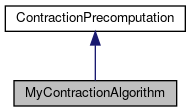
\includegraphics[width=215pt]{class_my_contraction_algorithm__inherit__graph}
\end{center}
\end{figure}


Collaboration diagram for My\+Contraction\+Algorithm\+:\nopagebreak
\begin{figure}[H]
\begin{center}
\leavevmode
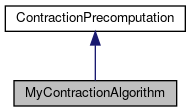
\includegraphics[width=215pt]{class_my_contraction_algorithm__coll__graph}
\end{center}
\end{figure}
\subsection*{Public Member Functions}
\begin{DoxyCompactItemize}
\item 
void \hyperlink{class_my_contraction_algorithm_a27a3be7ca9335a48ad08101c045bb883}{get\+Strongs} (const \hyperlink{pl__reff_8cpp_a65aea14f39d53b24df9910d54216d620}{Graph\+\_\+t} \&graph, const Graph\+\_\+t\+::\+Arc\+Map$<$ double $>$ \&l\+\_\+min, const Graph\+\_\+t\+::\+Arc\+Map$<$ double $>$ \&l\+\_\+max, Graph\+\_\+t\+::\+Arc uv, std\+::vector$<$ Graph\+\_\+t\+::\+Node $>$ \&strong\+\_\+nodes) const
\item 
void \hyperlink{class_my_contraction_algorithm_a7163cb16dd44d41e7a1974ed9f367e8a}{get\+Non\+Weaks} (const \hyperlink{pl__reff_8cpp_a65aea14f39d53b24df9910d54216d620}{Graph\+\_\+t} \&graph, const Graph\+\_\+t\+::\+Arc\+Map$<$ double $>$ \&l\+\_\+min, const Graph\+\_\+t\+::\+Arc\+Map$<$ double $>$ \&l\+\_\+max, Graph\+\_\+t\+::\+Arc uv, std\+::vector$<$ Graph\+\_\+t\+::\+Node $>$ \&non\+\_\+weak\+\_\+nodes) const
\item 
\hyperlink{class_contraction_result}{Contraction\+Result} \hyperlink{class_my_contraction_algorithm_ab2d761789cb18c240f5a610a9770ef29}{contract} (const \hyperlink{class_landscape}{Landscape} \&landscape, const \hyperlink{class_restoration_plan}{Restoration\+Plan} \&plan, Graph\+\_\+t\+::\+Node t, const std\+::vector$<$ Graph\+\_\+t\+::\+Arc $>$ \&contractables\+\_\+arcs, const std\+::vector$<$ Graph\+\_\+t\+::\+Arc $>$ \&orig\+\_\+deletables\+\_\+arcs) const
\item 
Graph\+\_\+t\+::\+Node\+Map$<$ \hyperlink{class_contraction_result}{Contraction\+Result} $>$ $\ast$ \hyperlink{class_my_contraction_algorithm_a4583c564e68d337bd9dcef315093bbe6}{precompute} (const \hyperlink{class_landscape}{Landscape} \&landscape, const \hyperlink{class_restoration_plan}{Restoration\+Plan} \&plan) const
\end{DoxyCompactItemize}


\subsection{Member Function Documentation}
\mbox{\Hypertarget{class_my_contraction_algorithm_ab2d761789cb18c240f5a610a9770ef29}\label{class_my_contraction_algorithm_ab2d761789cb18c240f5a610a9770ef29}} 
\index{My\+Contraction\+Algorithm@{My\+Contraction\+Algorithm}!contract@{contract}}
\index{contract@{contract}!My\+Contraction\+Algorithm@{My\+Contraction\+Algorithm}}
\subsubsection{\texorpdfstring{contract()}{contract()}}
{\footnotesize\ttfamily \hyperlink{class_contraction_result}{Contraction\+Result} My\+Contraction\+Algorithm\+::contract (\begin{DoxyParamCaption}\item[{const \hyperlink{class_landscape}{Landscape} \&}]{landscape,  }\item[{const \hyperlink{class_restoration_plan}{Restoration\+Plan} \&}]{plan,  }\item[{Graph\+\_\+t\+::\+Node}]{t,  }\item[{const std\+::vector$<$ Graph\+\_\+t\+::\+Arc $>$ \&}]{contractables\+\_\+arcs,  }\item[{const std\+::vector$<$ Graph\+\_\+t\+::\+Arc $>$ \&}]{orig\+\_\+deletables\+\_\+arcs }\end{DoxyParamCaption}) const}

\mbox{\Hypertarget{class_my_contraction_algorithm_a7163cb16dd44d41e7a1974ed9f367e8a}\label{class_my_contraction_algorithm_a7163cb16dd44d41e7a1974ed9f367e8a}} 
\index{My\+Contraction\+Algorithm@{My\+Contraction\+Algorithm}!get\+Non\+Weaks@{get\+Non\+Weaks}}
\index{get\+Non\+Weaks@{get\+Non\+Weaks}!My\+Contraction\+Algorithm@{My\+Contraction\+Algorithm}}
\subsubsection{\texorpdfstring{get\+Non\+Weaks()}{getNonWeaks()}}
{\footnotesize\ttfamily void My\+Contraction\+Algorithm\+::get\+Non\+Weaks (\begin{DoxyParamCaption}\item[{const \hyperlink{pl__reff_8cpp_a65aea14f39d53b24df9910d54216d620}{Graph\+\_\+t} \&}]{graph,  }\item[{const Graph\+\_\+t\+::\+Arc\+Map$<$ double $>$ \&}]{l\+\_\+min,  }\item[{const Graph\+\_\+t\+::\+Arc\+Map$<$ double $>$ \&}]{l\+\_\+max,  }\item[{Graph\+\_\+t\+::\+Arc}]{uv,  }\item[{std\+::vector$<$ Graph\+\_\+t\+::\+Node $>$ \&}]{non\+\_\+weak\+\_\+nodes }\end{DoxyParamCaption}) const}

\mbox{\Hypertarget{class_my_contraction_algorithm_a27a3be7ca9335a48ad08101c045bb883}\label{class_my_contraction_algorithm_a27a3be7ca9335a48ad08101c045bb883}} 
\index{My\+Contraction\+Algorithm@{My\+Contraction\+Algorithm}!get\+Strongs@{get\+Strongs}}
\index{get\+Strongs@{get\+Strongs}!My\+Contraction\+Algorithm@{My\+Contraction\+Algorithm}}
\subsubsection{\texorpdfstring{get\+Strongs()}{getStrongs()}}
{\footnotesize\ttfamily void My\+Contraction\+Algorithm\+::get\+Strongs (\begin{DoxyParamCaption}\item[{const \hyperlink{pl__reff_8cpp_a65aea14f39d53b24df9910d54216d620}{Graph\+\_\+t} \&}]{graph,  }\item[{const Graph\+\_\+t\+::\+Arc\+Map$<$ double $>$ \&}]{l\+\_\+min,  }\item[{const Graph\+\_\+t\+::\+Arc\+Map$<$ double $>$ \&}]{l\+\_\+max,  }\item[{Graph\+\_\+t\+::\+Arc}]{uv,  }\item[{std\+::vector$<$ Graph\+\_\+t\+::\+Node $>$ \&}]{strong\+\_\+nodes }\end{DoxyParamCaption}) const}

\mbox{\Hypertarget{class_my_contraction_algorithm_a4583c564e68d337bd9dcef315093bbe6}\label{class_my_contraction_algorithm_a4583c564e68d337bd9dcef315093bbe6}} 
\index{My\+Contraction\+Algorithm@{My\+Contraction\+Algorithm}!precompute@{precompute}}
\index{precompute@{precompute}!My\+Contraction\+Algorithm@{My\+Contraction\+Algorithm}}
\subsubsection{\texorpdfstring{precompute()}{precompute()}}
{\footnotesize\ttfamily Graph\+\_\+t\+::\+Node\+Map$<$ \hyperlink{class_contraction_result}{Contraction\+Result} $>$ $\ast$ My\+Contraction\+Algorithm\+::precompute (\begin{DoxyParamCaption}\item[{const \hyperlink{class_landscape}{Landscape} \&}]{landscape,  }\item[{const \hyperlink{class_restoration_plan}{Restoration\+Plan} \&}]{plan }\end{DoxyParamCaption}) const\hspace{0.3cm}{\ttfamily [virtual]}}



Implements \hyperlink{class_contraction_precomputation_a205ee98224bfa783a7ab27d3a986468b}{Contraction\+Precomputation}.



The documentation for this class was generated from the following files\+:\begin{DoxyCompactItemize}
\item 
/home/plaiseek/\+Projects/landscape\+\_\+opt\+\_\+cpp/include/precomputation/\hyperlink{my__contraction__algorithm_8hpp}{my\+\_\+contraction\+\_\+algorithm.\+hpp}\item 
/home/plaiseek/\+Projects/landscape\+\_\+opt\+\_\+cpp/src/precomputation/\hyperlink{my__contraction__algorithm_8cpp}{my\+\_\+contraction\+\_\+algorithm.\+cpp}\end{DoxyCompactItemize}

\hypertarget{class_solvers_1_1_naive___e_c_a___dec}{}\section{Solvers\+:\+:Naive\+\_\+\+E\+C\+A\+\_\+\+Dec Class Reference}
\label{class_solvers_1_1_naive___e_c_a___dec}\index{Solvers\+::\+Naive\+\_\+\+E\+C\+A\+\_\+\+Dec@{Solvers\+::\+Naive\+\_\+\+E\+C\+A\+\_\+\+Dec}}


{\ttfamily \#include $<$naive\+\_\+eca\+\_\+dec.\+hpp$>$}



Inheritance diagram for Solvers\+:\+:Naive\+\_\+\+E\+C\+A\+\_\+\+Dec\+:\nopagebreak
\begin{figure}[H]
\begin{center}
\leavevmode
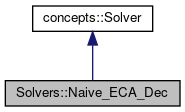
\includegraphics[width=211pt]{class_solvers_1_1_naive___e_c_a___dec__inherit__graph}
\end{center}
\end{figure}


Collaboration diagram for Solvers\+:\+:Naive\+\_\+\+E\+C\+A\+\_\+\+Dec\+:\nopagebreak
\begin{figure}[H]
\begin{center}
\leavevmode
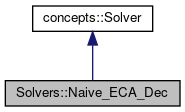
\includegraphics[width=211pt]{class_solvers_1_1_naive___e_c_a___dec__coll__graph}
\end{center}
\end{figure}
\subsection*{Public Member Functions}
\begin{DoxyCompactItemize}
\item 
\hyperlink{class_solvers_1_1_naive___e_c_a___dec_a31cb672115fcedb0f63c581ba3ccebdf}{Naive\+\_\+\+E\+C\+A\+\_\+\+Dec} ()
\item 
\hyperlink{class_solvers_1_1_naive___e_c_a___dec}{Naive\+\_\+\+E\+C\+A\+\_\+\+Dec} \& \hyperlink{class_solvers_1_1_naive___e_c_a___dec_a0a59573a3561ceaace10e38f282edc29}{set\+Log\+Level} (int log\+\_\+level)
\item 
\hyperlink{class_solvers_1_1_naive___e_c_a___dec}{Naive\+\_\+\+E\+C\+A\+\_\+\+Dec} \& \hyperlink{class_solvers_1_1_naive___e_c_a___dec_aac2179b8caf2d83ffd5cd63531be81aa}{set\+Parallel} (int parallel)
\item 
\hyperlink{class_solution}{Solution} $\ast$ \hyperlink{class_solvers_1_1_naive___e_c_a___dec_a51e13c5f7dac3c937f1a006c8b651657}{solve} (const \hyperlink{class_landscape}{Landscape} \&landscape, const \hyperlink{class_restoration_plan}{Restoration\+Plan} \&plan, const double B) const
\item 
const std\+::string \hyperlink{class_solvers_1_1_naive___e_c_a___dec_a171d5188c9901c251c57efdc9c8b954b}{name} () const
\end{DoxyCompactItemize}
\subsection*{Additional Inherited Members}


\subsection{Constructor \& Destructor Documentation}
\mbox{\Hypertarget{class_solvers_1_1_naive___e_c_a___dec_a31cb672115fcedb0f63c581ba3ccebdf}\label{class_solvers_1_1_naive___e_c_a___dec_a31cb672115fcedb0f63c581ba3ccebdf}} 
\index{Solvers\+::\+Naive\+\_\+\+E\+C\+A\+\_\+\+Dec@{Solvers\+::\+Naive\+\_\+\+E\+C\+A\+\_\+\+Dec}!Naive\+\_\+\+E\+C\+A\+\_\+\+Dec@{Naive\+\_\+\+E\+C\+A\+\_\+\+Dec}}
\index{Naive\+\_\+\+E\+C\+A\+\_\+\+Dec@{Naive\+\_\+\+E\+C\+A\+\_\+\+Dec}!Solvers\+::\+Naive\+\_\+\+E\+C\+A\+\_\+\+Dec@{Solvers\+::\+Naive\+\_\+\+E\+C\+A\+\_\+\+Dec}}
\subsubsection{\texorpdfstring{Naive\+\_\+\+E\+C\+A\+\_\+\+Dec()}{Naive\_ECA\_Dec()}}
{\footnotesize\ttfamily Solvers\+::\+Naive\+\_\+\+E\+C\+A\+\_\+\+Dec\+::\+Naive\+\_\+\+E\+C\+A\+\_\+\+Dec (\begin{DoxyParamCaption}{ }\end{DoxyParamCaption})\hspace{0.3cm}{\ttfamily [inline]}}



\subsection{Member Function Documentation}
\mbox{\Hypertarget{class_solvers_1_1_naive___e_c_a___dec_a171d5188c9901c251c57efdc9c8b954b}\label{class_solvers_1_1_naive___e_c_a___dec_a171d5188c9901c251c57efdc9c8b954b}} 
\index{Solvers\+::\+Naive\+\_\+\+E\+C\+A\+\_\+\+Dec@{Solvers\+::\+Naive\+\_\+\+E\+C\+A\+\_\+\+Dec}!name@{name}}
\index{name@{name}!Solvers\+::\+Naive\+\_\+\+E\+C\+A\+\_\+\+Dec@{Solvers\+::\+Naive\+\_\+\+E\+C\+A\+\_\+\+Dec}}
\subsubsection{\texorpdfstring{name()}{name()}}
{\footnotesize\ttfamily const std\+::string Solvers\+::\+Naive\+\_\+\+E\+C\+A\+\_\+\+Dec\+::name (\begin{DoxyParamCaption}{ }\end{DoxyParamCaption}) const\hspace{0.3cm}{\ttfamily [inline]}, {\ttfamily [virtual]}}



Implements \hyperlink{classconcepts_1_1_solver_ab995568318a506446228f45cab2fcce7}{concepts\+::\+Solver}.

\mbox{\Hypertarget{class_solvers_1_1_naive___e_c_a___dec_a0a59573a3561ceaace10e38f282edc29}\label{class_solvers_1_1_naive___e_c_a___dec_a0a59573a3561ceaace10e38f282edc29}} 
\index{Solvers\+::\+Naive\+\_\+\+E\+C\+A\+\_\+\+Dec@{Solvers\+::\+Naive\+\_\+\+E\+C\+A\+\_\+\+Dec}!set\+Log\+Level@{set\+Log\+Level}}
\index{set\+Log\+Level@{set\+Log\+Level}!Solvers\+::\+Naive\+\_\+\+E\+C\+A\+\_\+\+Dec@{Solvers\+::\+Naive\+\_\+\+E\+C\+A\+\_\+\+Dec}}
\subsubsection{\texorpdfstring{set\+Log\+Level()}{setLogLevel()}}
{\footnotesize\ttfamily \hyperlink{class_solvers_1_1_naive___e_c_a___dec}{Naive\+\_\+\+E\+C\+A\+\_\+\+Dec}\& Solvers\+::\+Naive\+\_\+\+E\+C\+A\+\_\+\+Dec\+::set\+Log\+Level (\begin{DoxyParamCaption}\item[{int}]{log\+\_\+level }\end{DoxyParamCaption})\hspace{0.3cm}{\ttfamily [inline]}}

\mbox{\Hypertarget{class_solvers_1_1_naive___e_c_a___dec_aac2179b8caf2d83ffd5cd63531be81aa}\label{class_solvers_1_1_naive___e_c_a___dec_aac2179b8caf2d83ffd5cd63531be81aa}} 
\index{Solvers\+::\+Naive\+\_\+\+E\+C\+A\+\_\+\+Dec@{Solvers\+::\+Naive\+\_\+\+E\+C\+A\+\_\+\+Dec}!set\+Parallel@{set\+Parallel}}
\index{set\+Parallel@{set\+Parallel}!Solvers\+::\+Naive\+\_\+\+E\+C\+A\+\_\+\+Dec@{Solvers\+::\+Naive\+\_\+\+E\+C\+A\+\_\+\+Dec}}
\subsubsection{\texorpdfstring{set\+Parallel()}{setParallel()}}
{\footnotesize\ttfamily \hyperlink{class_solvers_1_1_naive___e_c_a___dec}{Naive\+\_\+\+E\+C\+A\+\_\+\+Dec}\& Solvers\+::\+Naive\+\_\+\+E\+C\+A\+\_\+\+Dec\+::set\+Parallel (\begin{DoxyParamCaption}\item[{int}]{parallel }\end{DoxyParamCaption})\hspace{0.3cm}{\ttfamily [inline]}}

\mbox{\Hypertarget{class_solvers_1_1_naive___e_c_a___dec_a51e13c5f7dac3c937f1a006c8b651657}\label{class_solvers_1_1_naive___e_c_a___dec_a51e13c5f7dac3c937f1a006c8b651657}} 
\index{Solvers\+::\+Naive\+\_\+\+E\+C\+A\+\_\+\+Dec@{Solvers\+::\+Naive\+\_\+\+E\+C\+A\+\_\+\+Dec}!solve@{solve}}
\index{solve@{solve}!Solvers\+::\+Naive\+\_\+\+E\+C\+A\+\_\+\+Dec@{Solvers\+::\+Naive\+\_\+\+E\+C\+A\+\_\+\+Dec}}
\subsubsection{\texorpdfstring{solve()}{solve()}}
{\footnotesize\ttfamily \hyperlink{class_solution}{Solution} $\ast$ Solvers\+::\+Naive\+\_\+\+E\+C\+A\+\_\+\+Dec\+::solve (\begin{DoxyParamCaption}\item[{const \hyperlink{class_landscape}{Landscape} \&}]{landscape,  }\item[{const \hyperlink{class_restoration_plan}{Restoration\+Plan} \&}]{plan,  }\item[{const double}]{B }\end{DoxyParamCaption}) const\hspace{0.3cm}{\ttfamily [virtual]}}



Implements \hyperlink{classconcepts_1_1_solver_af323ad29df1e7b87facd7dc007568c80}{concepts\+::\+Solver}.



The documentation for this class was generated from the following files\+:\begin{DoxyCompactItemize}
\item 
/home/plaiseek/\+Projects/landscape\+\_\+opt\+\_\+cpp/include/solvers/\hyperlink{naive__eca__dec_8hpp}{naive\+\_\+eca\+\_\+dec.\+hpp}\item 
/home/plaiseek/\+Projects/landscape\+\_\+opt\+\_\+cpp/src/solvers/\hyperlink{naive__eca__dec_8cpp}{naive\+\_\+eca\+\_\+dec.\+cpp}\end{DoxyCompactItemize}

\hypertarget{class_solvers_1_1_naive___e_c_a___inc}{}\section{Solvers\+:\+:Naive\+\_\+\+E\+C\+A\+\_\+\+Inc Class Reference}
\label{class_solvers_1_1_naive___e_c_a___inc}\index{Solvers\+::\+Naive\+\_\+\+E\+C\+A\+\_\+\+Inc@{Solvers\+::\+Naive\+\_\+\+E\+C\+A\+\_\+\+Inc}}


{\ttfamily \#include $<$naive\+\_\+eca\+\_\+inc.\+hpp$>$}



Inheritance diagram for Solvers\+:\+:Naive\+\_\+\+E\+C\+A\+\_\+\+Inc\+:\nopagebreak
\begin{figure}[H]
\begin{center}
\leavevmode
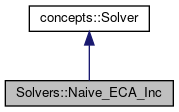
\includegraphics[width=206pt]{class_solvers_1_1_naive___e_c_a___inc__inherit__graph}
\end{center}
\end{figure}


Collaboration diagram for Solvers\+:\+:Naive\+\_\+\+E\+C\+A\+\_\+\+Inc\+:\nopagebreak
\begin{figure}[H]
\begin{center}
\leavevmode
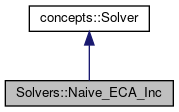
\includegraphics[width=206pt]{class_solvers_1_1_naive___e_c_a___inc__coll__graph}
\end{center}
\end{figure}
\subsection*{Public Member Functions}
\begin{DoxyCompactItemize}
\item 
\hyperlink{class_solvers_1_1_naive___e_c_a___inc_afca996d30836e4e6192373e00d6ed39f}{Naive\+\_\+\+E\+C\+A\+\_\+\+Inc} ()
\item 
\hyperlink{class_solvers_1_1_naive___e_c_a___inc}{Naive\+\_\+\+E\+C\+A\+\_\+\+Inc} \& \hyperlink{class_solvers_1_1_naive___e_c_a___inc_aa9231733d9dbc55a6f61a3811a3ebac1}{set\+Log\+Level} (int log\+\_\+level)
\item 
\hyperlink{class_solvers_1_1_naive___e_c_a___inc}{Naive\+\_\+\+E\+C\+A\+\_\+\+Inc} \& \hyperlink{class_solvers_1_1_naive___e_c_a___inc_a92d4284d10fd5d001a6ace0420361e5a}{set\+Parallel} (int parallel)
\item 
\hyperlink{class_solution}{Solution} $\ast$ \hyperlink{class_solvers_1_1_naive___e_c_a___inc_af0830eeb54be59ae2f363a32f38cee0c}{solve} (const \hyperlink{class_landscape}{Landscape} \&landscape, const \hyperlink{class_restoration_plan}{Restoration\+Plan} \&plan, const double B) const
\item 
const std\+::string \hyperlink{class_solvers_1_1_naive___e_c_a___inc_ace6070af722e226fcd2f9b746cc12944}{name} () const
\end{DoxyCompactItemize}
\subsection*{Additional Inherited Members}


\subsection{Constructor \& Destructor Documentation}
\mbox{\Hypertarget{class_solvers_1_1_naive___e_c_a___inc_afca996d30836e4e6192373e00d6ed39f}\label{class_solvers_1_1_naive___e_c_a___inc_afca996d30836e4e6192373e00d6ed39f}} 
\index{Solvers\+::\+Naive\+\_\+\+E\+C\+A\+\_\+\+Inc@{Solvers\+::\+Naive\+\_\+\+E\+C\+A\+\_\+\+Inc}!Naive\+\_\+\+E\+C\+A\+\_\+\+Inc@{Naive\+\_\+\+E\+C\+A\+\_\+\+Inc}}
\index{Naive\+\_\+\+E\+C\+A\+\_\+\+Inc@{Naive\+\_\+\+E\+C\+A\+\_\+\+Inc}!Solvers\+::\+Naive\+\_\+\+E\+C\+A\+\_\+\+Inc@{Solvers\+::\+Naive\+\_\+\+E\+C\+A\+\_\+\+Inc}}
\subsubsection{\texorpdfstring{Naive\+\_\+\+E\+C\+A\+\_\+\+Inc()}{Naive\_ECA\_Inc()}}
{\footnotesize\ttfamily Solvers\+::\+Naive\+\_\+\+E\+C\+A\+\_\+\+Inc\+::\+Naive\+\_\+\+E\+C\+A\+\_\+\+Inc (\begin{DoxyParamCaption}{ }\end{DoxyParamCaption})\hspace{0.3cm}{\ttfamily [inline]}}



\subsection{Member Function Documentation}
\mbox{\Hypertarget{class_solvers_1_1_naive___e_c_a___inc_ace6070af722e226fcd2f9b746cc12944}\label{class_solvers_1_1_naive___e_c_a___inc_ace6070af722e226fcd2f9b746cc12944}} 
\index{Solvers\+::\+Naive\+\_\+\+E\+C\+A\+\_\+\+Inc@{Solvers\+::\+Naive\+\_\+\+E\+C\+A\+\_\+\+Inc}!name@{name}}
\index{name@{name}!Solvers\+::\+Naive\+\_\+\+E\+C\+A\+\_\+\+Inc@{Solvers\+::\+Naive\+\_\+\+E\+C\+A\+\_\+\+Inc}}
\subsubsection{\texorpdfstring{name()}{name()}}
{\footnotesize\ttfamily const std\+::string Solvers\+::\+Naive\+\_\+\+E\+C\+A\+\_\+\+Inc\+::name (\begin{DoxyParamCaption}{ }\end{DoxyParamCaption}) const\hspace{0.3cm}{\ttfamily [inline]}, {\ttfamily [virtual]}}



Implements \hyperlink{classconcepts_1_1_solver_ab995568318a506446228f45cab2fcce7}{concepts\+::\+Solver}.

\mbox{\Hypertarget{class_solvers_1_1_naive___e_c_a___inc_aa9231733d9dbc55a6f61a3811a3ebac1}\label{class_solvers_1_1_naive___e_c_a___inc_aa9231733d9dbc55a6f61a3811a3ebac1}} 
\index{Solvers\+::\+Naive\+\_\+\+E\+C\+A\+\_\+\+Inc@{Solvers\+::\+Naive\+\_\+\+E\+C\+A\+\_\+\+Inc}!set\+Log\+Level@{set\+Log\+Level}}
\index{set\+Log\+Level@{set\+Log\+Level}!Solvers\+::\+Naive\+\_\+\+E\+C\+A\+\_\+\+Inc@{Solvers\+::\+Naive\+\_\+\+E\+C\+A\+\_\+\+Inc}}
\subsubsection{\texorpdfstring{set\+Log\+Level()}{setLogLevel()}}
{\footnotesize\ttfamily \hyperlink{class_solvers_1_1_naive___e_c_a___inc}{Naive\+\_\+\+E\+C\+A\+\_\+\+Inc}\& Solvers\+::\+Naive\+\_\+\+E\+C\+A\+\_\+\+Inc\+::set\+Log\+Level (\begin{DoxyParamCaption}\item[{int}]{log\+\_\+level }\end{DoxyParamCaption})\hspace{0.3cm}{\ttfamily [inline]}}

\mbox{\Hypertarget{class_solvers_1_1_naive___e_c_a___inc_a92d4284d10fd5d001a6ace0420361e5a}\label{class_solvers_1_1_naive___e_c_a___inc_a92d4284d10fd5d001a6ace0420361e5a}} 
\index{Solvers\+::\+Naive\+\_\+\+E\+C\+A\+\_\+\+Inc@{Solvers\+::\+Naive\+\_\+\+E\+C\+A\+\_\+\+Inc}!set\+Parallel@{set\+Parallel}}
\index{set\+Parallel@{set\+Parallel}!Solvers\+::\+Naive\+\_\+\+E\+C\+A\+\_\+\+Inc@{Solvers\+::\+Naive\+\_\+\+E\+C\+A\+\_\+\+Inc}}
\subsubsection{\texorpdfstring{set\+Parallel()}{setParallel()}}
{\footnotesize\ttfamily \hyperlink{class_solvers_1_1_naive___e_c_a___inc}{Naive\+\_\+\+E\+C\+A\+\_\+\+Inc}\& Solvers\+::\+Naive\+\_\+\+E\+C\+A\+\_\+\+Inc\+::set\+Parallel (\begin{DoxyParamCaption}\item[{int}]{parallel }\end{DoxyParamCaption})\hspace{0.3cm}{\ttfamily [inline]}}

\mbox{\Hypertarget{class_solvers_1_1_naive___e_c_a___inc_af0830eeb54be59ae2f363a32f38cee0c}\label{class_solvers_1_1_naive___e_c_a___inc_af0830eeb54be59ae2f363a32f38cee0c}} 
\index{Solvers\+::\+Naive\+\_\+\+E\+C\+A\+\_\+\+Inc@{Solvers\+::\+Naive\+\_\+\+E\+C\+A\+\_\+\+Inc}!solve@{solve}}
\index{solve@{solve}!Solvers\+::\+Naive\+\_\+\+E\+C\+A\+\_\+\+Inc@{Solvers\+::\+Naive\+\_\+\+E\+C\+A\+\_\+\+Inc}}
\subsubsection{\texorpdfstring{solve()}{solve()}}
{\footnotesize\ttfamily \hyperlink{class_solution}{Solution} $\ast$ Solvers\+::\+Naive\+\_\+\+E\+C\+A\+\_\+\+Inc\+::solve (\begin{DoxyParamCaption}\item[{const \hyperlink{class_landscape}{Landscape} \&}]{landscape,  }\item[{const \hyperlink{class_restoration_plan}{Restoration\+Plan} \&}]{plan,  }\item[{const double}]{B }\end{DoxyParamCaption}) const\hspace{0.3cm}{\ttfamily [virtual]}}



Implements \hyperlink{classconcepts_1_1_solver_af323ad29df1e7b87facd7dc007568c80}{concepts\+::\+Solver}.



The documentation for this class was generated from the following files\+:\begin{DoxyCompactItemize}
\item 
/home/plaiseek/\+Projects/landscape\+\_\+opt\+\_\+cpp/include/solvers/\hyperlink{naive__eca__inc_8hpp}{naive\+\_\+eca\+\_\+inc.\+hpp}\item 
/home/plaiseek/\+Projects/landscape\+\_\+opt\+\_\+cpp/src/solvers/\hyperlink{naive__eca__inc_8cpp}{naive\+\_\+eca\+\_\+inc.\+cpp}\end{DoxyCompactItemize}

\hypertarget{class_node_dist}{}\section{Node\+Dist Class Reference}
\label{class_node_dist}\index{Node\+Dist@{Node\+Dist}}
\subsection*{Public Member Functions}
\begin{DoxyCompactItemize}
\item 
\hyperlink{class_node_dist_a8a756d7e58f75575ddc390228b01de6d}{Node\+Dist} ()
\item 
\hyperlink{class_node_dist_aa5fb8c1b973ebc583d68b9f9b2aa79a1}{Node\+Dist} (double \hyperlink{class_node_dist_a5fb5b79a3402236741cb30dc4197d01d}{d})
\item 
\hyperlink{class_node_dist_a637baaba0175576b8978ad3196e9e152}{Node\+Dist} (double \hyperlink{class_node_dist_a5fb5b79a3402236741cb30dc4197d01d}{d}, bool \hyperlink{class_node_dist_a47cf7839304cb579bf424c740105b504}{b})
\item 
bool \hyperlink{class_node_dist_a870c09fd5a0a479e48a80225ea272dce}{operator$<$} (const \hyperlink{class_node_dist}{Node\+Dist} o) const
\item 
bool \hyperlink{class_node_dist_a37d6967f24dcb319434820bec612d60b}{operator==} (const \hyperlink{class_node_dist}{Node\+Dist} o) const
\item 
bool \hyperlink{class_node_dist_a25302f8442909cd2f0b139736ebf6495}{operator$<$=} (const \hyperlink{class_node_dist}{Node\+Dist} o) const
\item 
bool \hyperlink{class_node_dist_a725a1c34f71222f72d78cad219401445}{operator$>$=} (const \hyperlink{class_node_dist}{Node\+Dist} o) const
\item 
bool \hyperlink{class_node_dist_a5b75f14b46a331069c659b28682599d9}{operator$>$} (const \hyperlink{class_node_dist}{Node\+Dist} o) const
\item 
bool \hyperlink{class_node_dist_aaf38ee32e58160dff2f04b30cb9d4a3f}{operator!=} (const \hyperlink{class_node_dist}{Node\+Dist} o) const
\item 
\hyperlink{class_node_dist}{Node\+Dist} \hyperlink{class_node_dist_a8c702c614546aa1d7ea579c2a8638dd5}{operator+} (const \hyperlink{class_node_dist}{Node\+Dist} o) const
\item 
\hyperlink{class_node_dist}{Node\+Dist} \& \hyperlink{class_node_dist_a0d35171b68fa4493f4cf65a421ee2682}{operator+=} (const \hyperlink{class_node_dist}{Node\+Dist} o)
\item 
\hyperlink{class_node_dist}{Node\+Dist} \& \hyperlink{class_node_dist_ac9fced75410273f578795dc15f132b50}{operator=} (const \hyperlink{class_node_dist}{Node\+Dist} o)
\end{DoxyCompactItemize}
\subsection*{Public Attributes}
\begin{DoxyCompactItemize}
\item 
double \hyperlink{class_node_dist_a5fb5b79a3402236741cb30dc4197d01d}{d}
\item 
bool \hyperlink{class_node_dist_a47cf7839304cb579bf424c740105b504}{b}
\end{DoxyCompactItemize}


\subsection{Constructor \& Destructor Documentation}
\mbox{\Hypertarget{class_node_dist_a8a756d7e58f75575ddc390228b01de6d}\label{class_node_dist_a8a756d7e58f75575ddc390228b01de6d}} 
\index{Node\+Dist@{Node\+Dist}!Node\+Dist@{Node\+Dist}}
\index{Node\+Dist@{Node\+Dist}!Node\+Dist@{Node\+Dist}}
\subsubsection{\texorpdfstring{Node\+Dist()}{NodeDist()}\hspace{0.1cm}{\footnotesize\ttfamily [1/3]}}
{\footnotesize\ttfamily Node\+Dist\+::\+Node\+Dist (\begin{DoxyParamCaption}{ }\end{DoxyParamCaption})\hspace{0.3cm}{\ttfamily [inline]}}

\mbox{\Hypertarget{class_node_dist_aa5fb8c1b973ebc583d68b9f9b2aa79a1}\label{class_node_dist_aa5fb8c1b973ebc583d68b9f9b2aa79a1}} 
\index{Node\+Dist@{Node\+Dist}!Node\+Dist@{Node\+Dist}}
\index{Node\+Dist@{Node\+Dist}!Node\+Dist@{Node\+Dist}}
\subsubsection{\texorpdfstring{Node\+Dist()}{NodeDist()}\hspace{0.1cm}{\footnotesize\ttfamily [2/3]}}
{\footnotesize\ttfamily Node\+Dist\+::\+Node\+Dist (\begin{DoxyParamCaption}\item[{double}]{d }\end{DoxyParamCaption})\hspace{0.3cm}{\ttfamily [inline]}}

\mbox{\Hypertarget{class_node_dist_a637baaba0175576b8978ad3196e9e152}\label{class_node_dist_a637baaba0175576b8978ad3196e9e152}} 
\index{Node\+Dist@{Node\+Dist}!Node\+Dist@{Node\+Dist}}
\index{Node\+Dist@{Node\+Dist}!Node\+Dist@{Node\+Dist}}
\subsubsection{\texorpdfstring{Node\+Dist()}{NodeDist()}\hspace{0.1cm}{\footnotesize\ttfamily [3/3]}}
{\footnotesize\ttfamily Node\+Dist\+::\+Node\+Dist (\begin{DoxyParamCaption}\item[{double}]{d,  }\item[{bool}]{b }\end{DoxyParamCaption})\hspace{0.3cm}{\ttfamily [inline]}}



\subsection{Member Function Documentation}
\mbox{\Hypertarget{class_node_dist_aaf38ee32e58160dff2f04b30cb9d4a3f}\label{class_node_dist_aaf38ee32e58160dff2f04b30cb9d4a3f}} 
\index{Node\+Dist@{Node\+Dist}!operator"!=@{operator"!=}}
\index{operator"!=@{operator"!=}!Node\+Dist@{Node\+Dist}}
\subsubsection{\texorpdfstring{operator"!=()}{operator!=()}}
{\footnotesize\ttfamily bool Node\+Dist\+::operator!= (\begin{DoxyParamCaption}\item[{const \hyperlink{class_node_dist}{Node\+Dist}}]{o }\end{DoxyParamCaption}) const\hspace{0.3cm}{\ttfamily [inline]}}

\mbox{\Hypertarget{class_node_dist_a8c702c614546aa1d7ea579c2a8638dd5}\label{class_node_dist_a8c702c614546aa1d7ea579c2a8638dd5}} 
\index{Node\+Dist@{Node\+Dist}!operator+@{operator+}}
\index{operator+@{operator+}!Node\+Dist@{Node\+Dist}}
\subsubsection{\texorpdfstring{operator+()}{operator+()}}
{\footnotesize\ttfamily \hyperlink{class_node_dist}{Node\+Dist} Node\+Dist\+::operator+ (\begin{DoxyParamCaption}\item[{const \hyperlink{class_node_dist}{Node\+Dist}}]{o }\end{DoxyParamCaption}) const\hspace{0.3cm}{\ttfamily [inline]}}

\mbox{\Hypertarget{class_node_dist_a0d35171b68fa4493f4cf65a421ee2682}\label{class_node_dist_a0d35171b68fa4493f4cf65a421ee2682}} 
\index{Node\+Dist@{Node\+Dist}!operator+=@{operator+=}}
\index{operator+=@{operator+=}!Node\+Dist@{Node\+Dist}}
\subsubsection{\texorpdfstring{operator+=()}{operator+=()}}
{\footnotesize\ttfamily \hyperlink{class_node_dist}{Node\+Dist}\& Node\+Dist\+::operator+= (\begin{DoxyParamCaption}\item[{const \hyperlink{class_node_dist}{Node\+Dist}}]{o }\end{DoxyParamCaption})\hspace{0.3cm}{\ttfamily [inline]}}

\mbox{\Hypertarget{class_node_dist_a870c09fd5a0a479e48a80225ea272dce}\label{class_node_dist_a870c09fd5a0a479e48a80225ea272dce}} 
\index{Node\+Dist@{Node\+Dist}!operator$<$@{operator$<$}}
\index{operator$<$@{operator$<$}!Node\+Dist@{Node\+Dist}}
\subsubsection{\texorpdfstring{operator$<$()}{operator<()}}
{\footnotesize\ttfamily bool Node\+Dist\+::operator$<$ (\begin{DoxyParamCaption}\item[{const \hyperlink{class_node_dist}{Node\+Dist}}]{o }\end{DoxyParamCaption}) const\hspace{0.3cm}{\ttfamily [inline]}}

\mbox{\Hypertarget{class_node_dist_a25302f8442909cd2f0b139736ebf6495}\label{class_node_dist_a25302f8442909cd2f0b139736ebf6495}} 
\index{Node\+Dist@{Node\+Dist}!operator$<$=@{operator$<$=}}
\index{operator$<$=@{operator$<$=}!Node\+Dist@{Node\+Dist}}
\subsubsection{\texorpdfstring{operator$<$=()}{operator<=()}}
{\footnotesize\ttfamily bool Node\+Dist\+::operator$<$= (\begin{DoxyParamCaption}\item[{const \hyperlink{class_node_dist}{Node\+Dist}}]{o }\end{DoxyParamCaption}) const\hspace{0.3cm}{\ttfamily [inline]}}

\mbox{\Hypertarget{class_node_dist_ac9fced75410273f578795dc15f132b50}\label{class_node_dist_ac9fced75410273f578795dc15f132b50}} 
\index{Node\+Dist@{Node\+Dist}!operator=@{operator=}}
\index{operator=@{operator=}!Node\+Dist@{Node\+Dist}}
\subsubsection{\texorpdfstring{operator=()}{operator=()}}
{\footnotesize\ttfamily \hyperlink{class_node_dist}{Node\+Dist}\& Node\+Dist\+::operator= (\begin{DoxyParamCaption}\item[{const \hyperlink{class_node_dist}{Node\+Dist}}]{o }\end{DoxyParamCaption})\hspace{0.3cm}{\ttfamily [inline]}}

\mbox{\Hypertarget{class_node_dist_a37d6967f24dcb319434820bec612d60b}\label{class_node_dist_a37d6967f24dcb319434820bec612d60b}} 
\index{Node\+Dist@{Node\+Dist}!operator==@{operator==}}
\index{operator==@{operator==}!Node\+Dist@{Node\+Dist}}
\subsubsection{\texorpdfstring{operator==()}{operator==()}}
{\footnotesize\ttfamily bool Node\+Dist\+::operator== (\begin{DoxyParamCaption}\item[{const \hyperlink{class_node_dist}{Node\+Dist}}]{o }\end{DoxyParamCaption}) const\hspace{0.3cm}{\ttfamily [inline]}}

\mbox{\Hypertarget{class_node_dist_a5b75f14b46a331069c659b28682599d9}\label{class_node_dist_a5b75f14b46a331069c659b28682599d9}} 
\index{Node\+Dist@{Node\+Dist}!operator$>$@{operator$>$}}
\index{operator$>$@{operator$>$}!Node\+Dist@{Node\+Dist}}
\subsubsection{\texorpdfstring{operator$>$()}{operator>()}}
{\footnotesize\ttfamily bool Node\+Dist\+::operator$>$ (\begin{DoxyParamCaption}\item[{const \hyperlink{class_node_dist}{Node\+Dist}}]{o }\end{DoxyParamCaption}) const\hspace{0.3cm}{\ttfamily [inline]}}

\mbox{\Hypertarget{class_node_dist_a725a1c34f71222f72d78cad219401445}\label{class_node_dist_a725a1c34f71222f72d78cad219401445}} 
\index{Node\+Dist@{Node\+Dist}!operator$>$=@{operator$>$=}}
\index{operator$>$=@{operator$>$=}!Node\+Dist@{Node\+Dist}}
\subsubsection{\texorpdfstring{operator$>$=()}{operator>=()}}
{\footnotesize\ttfamily bool Node\+Dist\+::operator$>$= (\begin{DoxyParamCaption}\item[{const \hyperlink{class_node_dist}{Node\+Dist}}]{o }\end{DoxyParamCaption}) const\hspace{0.3cm}{\ttfamily [inline]}}



\subsection{Member Data Documentation}
\mbox{\Hypertarget{class_node_dist_a47cf7839304cb579bf424c740105b504}\label{class_node_dist_a47cf7839304cb579bf424c740105b504}} 
\index{Node\+Dist@{Node\+Dist}!b@{b}}
\index{b@{b}!Node\+Dist@{Node\+Dist}}
\subsubsection{\texorpdfstring{b}{b}}
{\footnotesize\ttfamily bool Node\+Dist\+::b}

\mbox{\Hypertarget{class_node_dist_a5fb5b79a3402236741cb30dc4197d01d}\label{class_node_dist_a5fb5b79a3402236741cb30dc4197d01d}} 
\index{Node\+Dist@{Node\+Dist}!d@{d}}
\index{d@{d}!Node\+Dist@{Node\+Dist}}
\subsubsection{\texorpdfstring{d}{d}}
{\footnotesize\ttfamily double Node\+Dist\+::d}



The documentation for this class was generated from the following file\+:\begin{DoxyCompactItemize}
\item 
/home/plaiseek/\+Projects/landscape\+\_\+opt\+\_\+cpp/src/precomputation/\hyperlink{my__contraction__algorithm_8cpp}{my\+\_\+contraction\+\_\+algorithm.\+cpp}\end{DoxyCompactItemize}

\hypertarget{class_restoration_plan_1_1_option}{}\section{Restoration\+Plan\+:\+:Option Class Reference}
\label{class_restoration_plan_1_1_option}\index{Restoration\+Plan\+::\+Option@{Restoration\+Plan\+::\+Option}}


{\ttfamily \#include $<$restoration\+\_\+plan.\+hpp$>$}

\subsection*{Public Member Functions}
\begin{DoxyCompactItemize}
\item 
\hyperlink{class_restoration_plan_1_1_option_a4b7de810dc136d3f1b7b59b540e3ab14}{Option} (\hyperlink{class_restoration_plan}{Restoration\+Plan} \&plan)
\item 
\hyperlink{class_restoration_plan_1_1_option_a17c9e40390e7941a3a0c8ed7141368d0}{$\sim$\+Option} ()
\item 
void \hyperlink{class_restoration_plan_1_1_option_a2434271320cdaf7976da04226a8f208b}{set\+Id} (int \hyperlink{class_restoration_plan_1_1_option_a9f520746b161200657579a6129cbcce4}{id})
\item 
int \hyperlink{class_restoration_plan_1_1_option_a0e878ed51e916cd12e13ce7fd05fad97}{get\+Id} () const
\item 
int \hyperlink{class_restoration_plan_1_1_option_aad1504a5146f0d1428c2a1870191e9c9}{get\+Nb\+Nodes} () const
\item 
int \hyperlink{class_restoration_plan_1_1_option_a7e460f4f101387b3ab489e3d87781a18}{get\+Nb\+Arcs} () const
\item 
int \hyperlink{class_restoration_plan_1_1_option_a593c37bd6a3243b24a254cf76ba43740}{get\+Nb\+Elems} () const
\item 
bool \hyperlink{class_restoration_plan_1_1_option_a33732229ec8a18047c2c5fd2ab46f63f}{contains} (Graph\+\_\+t\+::\+Node v) const
\item 
bool \hyperlink{class_restoration_plan_1_1_option_a61e1263cd6baa63be17b39bcfc8d6228}{contains} (Graph\+\_\+t\+::\+Arc a) const
\item 
void \hyperlink{class_restoration_plan_1_1_option_a65c8bad73ea738fa9aa3e20800ae2e5a}{add\+Patch} (Graph\+\_\+t\+::\+Node v, double quality\+\_\+gain)
\item 
void \hyperlink{class_restoration_plan_1_1_option_ac6dedad7776f2fe6fb605ed608d5646b}{add\+Link} (Graph\+\_\+t\+::\+Arc a, double restored\+\_\+probability)
\item 
void \hyperlink{class_restoration_plan_1_1_option_a279099f3a15244829442c469dea34840}{set\+Cost} (double cost)
\item 
void \hyperlink{class_restoration_plan_1_1_option_a4062a520bf0ded7d03ec6c9b69725c06}{remove\+Patch} (Graph\+\_\+t\+::\+Node v)
\item 
void \hyperlink{class_restoration_plan_1_1_option_ac0f220ea195f37bf169a0cd73352d3cb}{remove\+Link} (Graph\+\_\+t\+::\+Arc a)
\item 
double \hyperlink{class_restoration_plan_1_1_option_a3b6e892cfd36a4612de5222bfcfb23ff}{get\+Quality\+Gain} (Graph\+\_\+t\+::\+Node v) const
\item 
double \hyperlink{class_restoration_plan_1_1_option_a498802305d2c9c421446c326b65a4028}{get\+Restored\+Probability} (Graph\+\_\+t\+::\+Arc a) const
\item 
double \hyperlink{class_restoration_plan_1_1_option_aee4ddb7bdf2b6caaebeb87e2055b5be1}{get\+Cost} () const
\item 
double \& \hyperlink{class_restoration_plan_1_1_option_ab38a032c7b9d0bfdd267e9ec2ff21caa}{get\+Quality\+Gain\+Ref} (Graph\+\_\+t\+::\+Node v)
\item 
double \& \hyperlink{class_restoration_plan_1_1_option_a07ddd47b0851f9470ba6d388f976d877}{get\+Restored\+Probability\+Ref} (Graph\+\_\+t\+::\+Arc a)
\item 
double \& \hyperlink{class_restoration_plan_1_1_option_a614e659b457b722ed61923c2e30f0f8c}{get\+Cost\+Ref} ()
\item 
int \hyperlink{class_restoration_plan_1_1_option_a9f520746b161200657579a6129cbcce4}{id} (Graph\+\_\+t\+::\+Node v) const
\item 
int \hyperlink{class_restoration_plan_1_1_option_a59a89db7f6e5f3fabadb57b89bd71932}{id} (Graph\+\_\+t\+::\+Arc a) const
\item 
const std\+::vector$<$ Graph\+\_\+t\+::\+Node $>$ \& \hyperlink{class_restoration_plan_1_1_option_a61190e5185ad1ccb3e1c4b546fdb02b4}{nodes} () const
\item 
const std\+::vector$<$ Graph\+\_\+t\+::\+Arc $>$ \& \hyperlink{class_restoration_plan_1_1_option_a59cc737c2525fa25f1f1241ea9e53d90}{arcs} () const
\item 
double \hyperlink{class_restoration_plan_1_1_option_a0174047c9abd2e325e5af813eeda3e58}{operator\mbox{[}$\,$\mbox{]}} (Graph\+\_\+t\+::\+Node v) const
\item 
double \hyperlink{class_restoration_plan_1_1_option_a9055a8d1eb192f0e588f20ffd26ed30a}{operator\mbox{[}$\,$\mbox{]}} (Graph\+\_\+t\+::\+Arc a) const
\item 
double \& \hyperlink{class_restoration_plan_1_1_option_a6b8531ca7119295af00743a0f4797dba}{operator\mbox{[}$\,$\mbox{]}} (Graph\+\_\+t\+::\+Node v)
\item 
double \& \hyperlink{class_restoration_plan_1_1_option_a9b78dc0b8b13778ce128f6b723aabdda}{operator\mbox{[}$\,$\mbox{]}} (Graph\+\_\+t\+::\+Arc a)
\end{DoxyCompactItemize}


\subsection{Constructor \& Destructor Documentation}
\mbox{\Hypertarget{class_restoration_plan_1_1_option_a4b7de810dc136d3f1b7b59b540e3ab14}\label{class_restoration_plan_1_1_option_a4b7de810dc136d3f1b7b59b540e3ab14}} 
\index{Restoration\+Plan\+::\+Option@{Restoration\+Plan\+::\+Option}!Option@{Option}}
\index{Option@{Option}!Restoration\+Plan\+::\+Option@{Restoration\+Plan\+::\+Option}}
\subsubsection{\texorpdfstring{Option()}{Option()}}
{\footnotesize\ttfamily Restoration\+Plan\+::\+Option\+::\+Option (\begin{DoxyParamCaption}\item[{\hyperlink{class_restoration_plan}{Restoration\+Plan} \&}]{plan }\end{DoxyParamCaption})}

\mbox{\Hypertarget{class_restoration_plan_1_1_option_a17c9e40390e7941a3a0c8ed7141368d0}\label{class_restoration_plan_1_1_option_a17c9e40390e7941a3a0c8ed7141368d0}} 
\index{Restoration\+Plan\+::\+Option@{Restoration\+Plan\+::\+Option}!````~Option@{$\sim$\+Option}}
\index{````~Option@{$\sim$\+Option}!Restoration\+Plan\+::\+Option@{Restoration\+Plan\+::\+Option}}
\subsubsection{\texorpdfstring{$\sim$\+Option()}{~Option()}}
{\footnotesize\ttfamily Restoration\+Plan\+::\+Option\+::$\sim$\+Option (\begin{DoxyParamCaption}{ }\end{DoxyParamCaption})}



\subsection{Member Function Documentation}
\mbox{\Hypertarget{class_restoration_plan_1_1_option_ac6dedad7776f2fe6fb605ed608d5646b}\label{class_restoration_plan_1_1_option_ac6dedad7776f2fe6fb605ed608d5646b}} 
\index{Restoration\+Plan\+::\+Option@{Restoration\+Plan\+::\+Option}!add\+Link@{add\+Link}}
\index{add\+Link@{add\+Link}!Restoration\+Plan\+::\+Option@{Restoration\+Plan\+::\+Option}}
\subsubsection{\texorpdfstring{add\+Link()}{addLink()}}
{\footnotesize\ttfamily void Restoration\+Plan\+::\+Option\+::add\+Link (\begin{DoxyParamCaption}\item[{Graph\+\_\+t\+::\+Arc}]{a,  }\item[{double}]{restored\+\_\+probability }\end{DoxyParamCaption})}

\mbox{\Hypertarget{class_restoration_plan_1_1_option_a65c8bad73ea738fa9aa3e20800ae2e5a}\label{class_restoration_plan_1_1_option_a65c8bad73ea738fa9aa3e20800ae2e5a}} 
\index{Restoration\+Plan\+::\+Option@{Restoration\+Plan\+::\+Option}!add\+Patch@{add\+Patch}}
\index{add\+Patch@{add\+Patch}!Restoration\+Plan\+::\+Option@{Restoration\+Plan\+::\+Option}}
\subsubsection{\texorpdfstring{add\+Patch()}{addPatch()}}
{\footnotesize\ttfamily void Restoration\+Plan\+::\+Option\+::add\+Patch (\begin{DoxyParamCaption}\item[{Graph\+\_\+t\+::\+Node}]{v,  }\item[{double}]{quality\+\_\+gain }\end{DoxyParamCaption})}

\mbox{\Hypertarget{class_restoration_plan_1_1_option_a59cc737c2525fa25f1f1241ea9e53d90}\label{class_restoration_plan_1_1_option_a59cc737c2525fa25f1f1241ea9e53d90}} 
\index{Restoration\+Plan\+::\+Option@{Restoration\+Plan\+::\+Option}!arcs@{arcs}}
\index{arcs@{arcs}!Restoration\+Plan\+::\+Option@{Restoration\+Plan\+::\+Option}}
\subsubsection{\texorpdfstring{arcs()}{arcs()}}
{\footnotesize\ttfamily const std\+::vector$<$ Graph\+\_\+t\+::\+Arc $>$ \& Restoration\+Plan\+::\+Option\+::arcs (\begin{DoxyParamCaption}{ }\end{DoxyParamCaption}) const}

\mbox{\Hypertarget{class_restoration_plan_1_1_option_a33732229ec8a18047c2c5fd2ab46f63f}\label{class_restoration_plan_1_1_option_a33732229ec8a18047c2c5fd2ab46f63f}} 
\index{Restoration\+Plan\+::\+Option@{Restoration\+Plan\+::\+Option}!contains@{contains}}
\index{contains@{contains}!Restoration\+Plan\+::\+Option@{Restoration\+Plan\+::\+Option}}
\subsubsection{\texorpdfstring{contains()}{contains()}\hspace{0.1cm}{\footnotesize\ttfamily [1/2]}}
{\footnotesize\ttfamily bool Restoration\+Plan\+::\+Option\+::contains (\begin{DoxyParamCaption}\item[{Graph\+\_\+t\+::\+Node}]{v }\end{DoxyParamCaption}) const}

\mbox{\Hypertarget{class_restoration_plan_1_1_option_a61e1263cd6baa63be17b39bcfc8d6228}\label{class_restoration_plan_1_1_option_a61e1263cd6baa63be17b39bcfc8d6228}} 
\index{Restoration\+Plan\+::\+Option@{Restoration\+Plan\+::\+Option}!contains@{contains}}
\index{contains@{contains}!Restoration\+Plan\+::\+Option@{Restoration\+Plan\+::\+Option}}
\subsubsection{\texorpdfstring{contains()}{contains()}\hspace{0.1cm}{\footnotesize\ttfamily [2/2]}}
{\footnotesize\ttfamily bool Restoration\+Plan\+::\+Option\+::contains (\begin{DoxyParamCaption}\item[{Graph\+\_\+t\+::\+Arc}]{a }\end{DoxyParamCaption}) const}

\mbox{\Hypertarget{class_restoration_plan_1_1_option_aee4ddb7bdf2b6caaebeb87e2055b5be1}\label{class_restoration_plan_1_1_option_aee4ddb7bdf2b6caaebeb87e2055b5be1}} 
\index{Restoration\+Plan\+::\+Option@{Restoration\+Plan\+::\+Option}!get\+Cost@{get\+Cost}}
\index{get\+Cost@{get\+Cost}!Restoration\+Plan\+::\+Option@{Restoration\+Plan\+::\+Option}}
\subsubsection{\texorpdfstring{get\+Cost()}{getCost()}}
{\footnotesize\ttfamily double Restoration\+Plan\+::\+Option\+::get\+Cost (\begin{DoxyParamCaption}{ }\end{DoxyParamCaption}) const}

\mbox{\Hypertarget{class_restoration_plan_1_1_option_a614e659b457b722ed61923c2e30f0f8c}\label{class_restoration_plan_1_1_option_a614e659b457b722ed61923c2e30f0f8c}} 
\index{Restoration\+Plan\+::\+Option@{Restoration\+Plan\+::\+Option}!get\+Cost\+Ref@{get\+Cost\+Ref}}
\index{get\+Cost\+Ref@{get\+Cost\+Ref}!Restoration\+Plan\+::\+Option@{Restoration\+Plan\+::\+Option}}
\subsubsection{\texorpdfstring{get\+Cost\+Ref()}{getCostRef()}}
{\footnotesize\ttfamily double \& Restoration\+Plan\+::\+Option\+::get\+Cost\+Ref (\begin{DoxyParamCaption}{ }\end{DoxyParamCaption})}

\mbox{\Hypertarget{class_restoration_plan_1_1_option_a0e878ed51e916cd12e13ce7fd05fad97}\label{class_restoration_plan_1_1_option_a0e878ed51e916cd12e13ce7fd05fad97}} 
\index{Restoration\+Plan\+::\+Option@{Restoration\+Plan\+::\+Option}!get\+Id@{get\+Id}}
\index{get\+Id@{get\+Id}!Restoration\+Plan\+::\+Option@{Restoration\+Plan\+::\+Option}}
\subsubsection{\texorpdfstring{get\+Id()}{getId()}}
{\footnotesize\ttfamily int Restoration\+Plan\+::\+Option\+::get\+Id (\begin{DoxyParamCaption}{ }\end{DoxyParamCaption}) const}

\mbox{\Hypertarget{class_restoration_plan_1_1_option_a7e460f4f101387b3ab489e3d87781a18}\label{class_restoration_plan_1_1_option_a7e460f4f101387b3ab489e3d87781a18}} 
\index{Restoration\+Plan\+::\+Option@{Restoration\+Plan\+::\+Option}!get\+Nb\+Arcs@{get\+Nb\+Arcs}}
\index{get\+Nb\+Arcs@{get\+Nb\+Arcs}!Restoration\+Plan\+::\+Option@{Restoration\+Plan\+::\+Option}}
\subsubsection{\texorpdfstring{get\+Nb\+Arcs()}{getNbArcs()}}
{\footnotesize\ttfamily int Restoration\+Plan\+::\+Option\+::get\+Nb\+Arcs (\begin{DoxyParamCaption}{ }\end{DoxyParamCaption}) const}

\mbox{\Hypertarget{class_restoration_plan_1_1_option_a593c37bd6a3243b24a254cf76ba43740}\label{class_restoration_plan_1_1_option_a593c37bd6a3243b24a254cf76ba43740}} 
\index{Restoration\+Plan\+::\+Option@{Restoration\+Plan\+::\+Option}!get\+Nb\+Elems@{get\+Nb\+Elems}}
\index{get\+Nb\+Elems@{get\+Nb\+Elems}!Restoration\+Plan\+::\+Option@{Restoration\+Plan\+::\+Option}}
\subsubsection{\texorpdfstring{get\+Nb\+Elems()}{getNbElems()}}
{\footnotesize\ttfamily int Restoration\+Plan\+::\+Option\+::get\+Nb\+Elems (\begin{DoxyParamCaption}{ }\end{DoxyParamCaption}) const}

\mbox{\Hypertarget{class_restoration_plan_1_1_option_aad1504a5146f0d1428c2a1870191e9c9}\label{class_restoration_plan_1_1_option_aad1504a5146f0d1428c2a1870191e9c9}} 
\index{Restoration\+Plan\+::\+Option@{Restoration\+Plan\+::\+Option}!get\+Nb\+Nodes@{get\+Nb\+Nodes}}
\index{get\+Nb\+Nodes@{get\+Nb\+Nodes}!Restoration\+Plan\+::\+Option@{Restoration\+Plan\+::\+Option}}
\subsubsection{\texorpdfstring{get\+Nb\+Nodes()}{getNbNodes()}}
{\footnotesize\ttfamily int Restoration\+Plan\+::\+Option\+::get\+Nb\+Nodes (\begin{DoxyParamCaption}{ }\end{DoxyParamCaption}) const}

\mbox{\Hypertarget{class_restoration_plan_1_1_option_a3b6e892cfd36a4612de5222bfcfb23ff}\label{class_restoration_plan_1_1_option_a3b6e892cfd36a4612de5222bfcfb23ff}} 
\index{Restoration\+Plan\+::\+Option@{Restoration\+Plan\+::\+Option}!get\+Quality\+Gain@{get\+Quality\+Gain}}
\index{get\+Quality\+Gain@{get\+Quality\+Gain}!Restoration\+Plan\+::\+Option@{Restoration\+Plan\+::\+Option}}
\subsubsection{\texorpdfstring{get\+Quality\+Gain()}{getQualityGain()}}
{\footnotesize\ttfamily double Restoration\+Plan\+::\+Option\+::get\+Quality\+Gain (\begin{DoxyParamCaption}\item[{Graph\+\_\+t\+::\+Node}]{v }\end{DoxyParamCaption}) const}

\mbox{\Hypertarget{class_restoration_plan_1_1_option_ab38a032c7b9d0bfdd267e9ec2ff21caa}\label{class_restoration_plan_1_1_option_ab38a032c7b9d0bfdd267e9ec2ff21caa}} 
\index{Restoration\+Plan\+::\+Option@{Restoration\+Plan\+::\+Option}!get\+Quality\+Gain\+Ref@{get\+Quality\+Gain\+Ref}}
\index{get\+Quality\+Gain\+Ref@{get\+Quality\+Gain\+Ref}!Restoration\+Plan\+::\+Option@{Restoration\+Plan\+::\+Option}}
\subsubsection{\texorpdfstring{get\+Quality\+Gain\+Ref()}{getQualityGainRef()}}
{\footnotesize\ttfamily double \& Restoration\+Plan\+::\+Option\+::get\+Quality\+Gain\+Ref (\begin{DoxyParamCaption}\item[{Graph\+\_\+t\+::\+Node}]{v }\end{DoxyParamCaption})}

\mbox{\Hypertarget{class_restoration_plan_1_1_option_a498802305d2c9c421446c326b65a4028}\label{class_restoration_plan_1_1_option_a498802305d2c9c421446c326b65a4028}} 
\index{Restoration\+Plan\+::\+Option@{Restoration\+Plan\+::\+Option}!get\+Restored\+Probability@{get\+Restored\+Probability}}
\index{get\+Restored\+Probability@{get\+Restored\+Probability}!Restoration\+Plan\+::\+Option@{Restoration\+Plan\+::\+Option}}
\subsubsection{\texorpdfstring{get\+Restored\+Probability()}{getRestoredProbability()}}
{\footnotesize\ttfamily double Restoration\+Plan\+::\+Option\+::get\+Restored\+Probability (\begin{DoxyParamCaption}\item[{Graph\+\_\+t\+::\+Arc}]{a }\end{DoxyParamCaption}) const}

\mbox{\Hypertarget{class_restoration_plan_1_1_option_a07ddd47b0851f9470ba6d388f976d877}\label{class_restoration_plan_1_1_option_a07ddd47b0851f9470ba6d388f976d877}} 
\index{Restoration\+Plan\+::\+Option@{Restoration\+Plan\+::\+Option}!get\+Restored\+Probability\+Ref@{get\+Restored\+Probability\+Ref}}
\index{get\+Restored\+Probability\+Ref@{get\+Restored\+Probability\+Ref}!Restoration\+Plan\+::\+Option@{Restoration\+Plan\+::\+Option}}
\subsubsection{\texorpdfstring{get\+Restored\+Probability\+Ref()}{getRestoredProbabilityRef()}}
{\footnotesize\ttfamily double \& Restoration\+Plan\+::\+Option\+::get\+Restored\+Probability\+Ref (\begin{DoxyParamCaption}\item[{Graph\+\_\+t\+::\+Arc}]{a }\end{DoxyParamCaption})}

\mbox{\Hypertarget{class_restoration_plan_1_1_option_a9f520746b161200657579a6129cbcce4}\label{class_restoration_plan_1_1_option_a9f520746b161200657579a6129cbcce4}} 
\index{Restoration\+Plan\+::\+Option@{Restoration\+Plan\+::\+Option}!id@{id}}
\index{id@{id}!Restoration\+Plan\+::\+Option@{Restoration\+Plan\+::\+Option}}
\subsubsection{\texorpdfstring{id()}{id()}\hspace{0.1cm}{\footnotesize\ttfamily [1/2]}}
{\footnotesize\ttfamily int Restoration\+Plan\+::\+Option\+::id (\begin{DoxyParamCaption}\item[{Graph\+\_\+t\+::\+Node}]{v }\end{DoxyParamCaption}) const}

\mbox{\Hypertarget{class_restoration_plan_1_1_option_a59a89db7f6e5f3fabadb57b89bd71932}\label{class_restoration_plan_1_1_option_a59a89db7f6e5f3fabadb57b89bd71932}} 
\index{Restoration\+Plan\+::\+Option@{Restoration\+Plan\+::\+Option}!id@{id}}
\index{id@{id}!Restoration\+Plan\+::\+Option@{Restoration\+Plan\+::\+Option}}
\subsubsection{\texorpdfstring{id()}{id()}\hspace{0.1cm}{\footnotesize\ttfamily [2/2]}}
{\footnotesize\ttfamily int Restoration\+Plan\+::\+Option\+::id (\begin{DoxyParamCaption}\item[{Graph\+\_\+t\+::\+Arc}]{a }\end{DoxyParamCaption}) const}

\mbox{\Hypertarget{class_restoration_plan_1_1_option_a61190e5185ad1ccb3e1c4b546fdb02b4}\label{class_restoration_plan_1_1_option_a61190e5185ad1ccb3e1c4b546fdb02b4}} 
\index{Restoration\+Plan\+::\+Option@{Restoration\+Plan\+::\+Option}!nodes@{nodes}}
\index{nodes@{nodes}!Restoration\+Plan\+::\+Option@{Restoration\+Plan\+::\+Option}}
\subsubsection{\texorpdfstring{nodes()}{nodes()}}
{\footnotesize\ttfamily const std\+::vector$<$ Graph\+\_\+t\+::\+Node $>$ \& Restoration\+Plan\+::\+Option\+::nodes (\begin{DoxyParamCaption}{ }\end{DoxyParamCaption}) const}

\mbox{\Hypertarget{class_restoration_plan_1_1_option_a0174047c9abd2e325e5af813eeda3e58}\label{class_restoration_plan_1_1_option_a0174047c9abd2e325e5af813eeda3e58}} 
\index{Restoration\+Plan\+::\+Option@{Restoration\+Plan\+::\+Option}!operator\mbox{[}\mbox{]}@{operator[]}}
\index{operator\mbox{[}\mbox{]}@{operator[]}!Restoration\+Plan\+::\+Option@{Restoration\+Plan\+::\+Option}}
\subsubsection{\texorpdfstring{operator[]()}{operator[]()}\hspace{0.1cm}{\footnotesize\ttfamily [1/4]}}
{\footnotesize\ttfamily double Restoration\+Plan\+::\+Option\+::operator\mbox{[}$\,$\mbox{]} (\begin{DoxyParamCaption}\item[{Graph\+\_\+t\+::\+Node}]{v }\end{DoxyParamCaption}) const}

\mbox{\Hypertarget{class_restoration_plan_1_1_option_a9055a8d1eb192f0e588f20ffd26ed30a}\label{class_restoration_plan_1_1_option_a9055a8d1eb192f0e588f20ffd26ed30a}} 
\index{Restoration\+Plan\+::\+Option@{Restoration\+Plan\+::\+Option}!operator\mbox{[}\mbox{]}@{operator[]}}
\index{operator\mbox{[}\mbox{]}@{operator[]}!Restoration\+Plan\+::\+Option@{Restoration\+Plan\+::\+Option}}
\subsubsection{\texorpdfstring{operator[]()}{operator[]()}\hspace{0.1cm}{\footnotesize\ttfamily [2/4]}}
{\footnotesize\ttfamily double Restoration\+Plan\+::\+Option\+::operator\mbox{[}$\,$\mbox{]} (\begin{DoxyParamCaption}\item[{Graph\+\_\+t\+::\+Arc}]{a }\end{DoxyParamCaption}) const}

\mbox{\Hypertarget{class_restoration_plan_1_1_option_a6b8531ca7119295af00743a0f4797dba}\label{class_restoration_plan_1_1_option_a6b8531ca7119295af00743a0f4797dba}} 
\index{Restoration\+Plan\+::\+Option@{Restoration\+Plan\+::\+Option}!operator\mbox{[}\mbox{]}@{operator[]}}
\index{operator\mbox{[}\mbox{]}@{operator[]}!Restoration\+Plan\+::\+Option@{Restoration\+Plan\+::\+Option}}
\subsubsection{\texorpdfstring{operator[]()}{operator[]()}\hspace{0.1cm}{\footnotesize\ttfamily [3/4]}}
{\footnotesize\ttfamily double \& Restoration\+Plan\+::\+Option\+::operator\mbox{[}$\,$\mbox{]} (\begin{DoxyParamCaption}\item[{Graph\+\_\+t\+::\+Node}]{v }\end{DoxyParamCaption})}

\mbox{\Hypertarget{class_restoration_plan_1_1_option_a9b78dc0b8b13778ce128f6b723aabdda}\label{class_restoration_plan_1_1_option_a9b78dc0b8b13778ce128f6b723aabdda}} 
\index{Restoration\+Plan\+::\+Option@{Restoration\+Plan\+::\+Option}!operator\mbox{[}\mbox{]}@{operator[]}}
\index{operator\mbox{[}\mbox{]}@{operator[]}!Restoration\+Plan\+::\+Option@{Restoration\+Plan\+::\+Option}}
\subsubsection{\texorpdfstring{operator[]()}{operator[]()}\hspace{0.1cm}{\footnotesize\ttfamily [4/4]}}
{\footnotesize\ttfamily double \& Restoration\+Plan\+::\+Option\+::operator\mbox{[}$\,$\mbox{]} (\begin{DoxyParamCaption}\item[{Graph\+\_\+t\+::\+Arc}]{a }\end{DoxyParamCaption})}

\mbox{\Hypertarget{class_restoration_plan_1_1_option_ac0f220ea195f37bf169a0cd73352d3cb}\label{class_restoration_plan_1_1_option_ac0f220ea195f37bf169a0cd73352d3cb}} 
\index{Restoration\+Plan\+::\+Option@{Restoration\+Plan\+::\+Option}!remove\+Link@{remove\+Link}}
\index{remove\+Link@{remove\+Link}!Restoration\+Plan\+::\+Option@{Restoration\+Plan\+::\+Option}}
\subsubsection{\texorpdfstring{remove\+Link()}{removeLink()}}
{\footnotesize\ttfamily void Restoration\+Plan\+::\+Option\+::remove\+Link (\begin{DoxyParamCaption}\item[{Graph\+\_\+t\+::\+Arc}]{a }\end{DoxyParamCaption})}

\mbox{\Hypertarget{class_restoration_plan_1_1_option_a4062a520bf0ded7d03ec6c9b69725c06}\label{class_restoration_plan_1_1_option_a4062a520bf0ded7d03ec6c9b69725c06}} 
\index{Restoration\+Plan\+::\+Option@{Restoration\+Plan\+::\+Option}!remove\+Patch@{remove\+Patch}}
\index{remove\+Patch@{remove\+Patch}!Restoration\+Plan\+::\+Option@{Restoration\+Plan\+::\+Option}}
\subsubsection{\texorpdfstring{remove\+Patch()}{removePatch()}}
{\footnotesize\ttfamily void Restoration\+Plan\+::\+Option\+::remove\+Patch (\begin{DoxyParamCaption}\item[{Graph\+\_\+t\+::\+Node}]{v }\end{DoxyParamCaption})}

\mbox{\Hypertarget{class_restoration_plan_1_1_option_a279099f3a15244829442c469dea34840}\label{class_restoration_plan_1_1_option_a279099f3a15244829442c469dea34840}} 
\index{Restoration\+Plan\+::\+Option@{Restoration\+Plan\+::\+Option}!set\+Cost@{set\+Cost}}
\index{set\+Cost@{set\+Cost}!Restoration\+Plan\+::\+Option@{Restoration\+Plan\+::\+Option}}
\subsubsection{\texorpdfstring{set\+Cost()}{setCost()}}
{\footnotesize\ttfamily void Restoration\+Plan\+::\+Option\+::set\+Cost (\begin{DoxyParamCaption}\item[{double}]{cost }\end{DoxyParamCaption})}

\mbox{\Hypertarget{class_restoration_plan_1_1_option_a2434271320cdaf7976da04226a8f208b}\label{class_restoration_plan_1_1_option_a2434271320cdaf7976da04226a8f208b}} 
\index{Restoration\+Plan\+::\+Option@{Restoration\+Plan\+::\+Option}!set\+Id@{set\+Id}}
\index{set\+Id@{set\+Id}!Restoration\+Plan\+::\+Option@{Restoration\+Plan\+::\+Option}}
\subsubsection{\texorpdfstring{set\+Id()}{setId()}}
{\footnotesize\ttfamily void Restoration\+Plan\+::\+Option\+::set\+Id (\begin{DoxyParamCaption}\item[{int}]{id }\end{DoxyParamCaption})}



The documentation for this class was generated from the following files\+:\begin{DoxyCompactItemize}
\item 
/home/plaiseek/\+Projects/landscape\+\_\+opt\+\_\+cpp/include/solvers/concept/\hyperlink{restoration__plan_8hpp}{restoration\+\_\+plan.\+hpp}\item 
/home/plaiseek/\+Projects/landscape\+\_\+opt\+\_\+cpp/src/solvers/concept/\hyperlink{restoration__option_8cpp}{restoration\+\_\+option.\+cpp}\end{DoxyCompactItemize}

\hypertarget{class_o_s_i___builder}{}\section{O\+S\+I\+\_\+\+Builder Class Reference}
\label{class_o_s_i___builder}\index{O\+S\+I\+\_\+\+Builder@{O\+S\+I\+\_\+\+Builder}}


A practical class for building Osi\+Solver instances.  




{\ttfamily \#include $<$osi\+\_\+builder.\+hpp$>$}

\subsection*{Classes}
\begin{DoxyCompactItemize}
\item 
class \hyperlink{class_o_s_i___builder_1_1_var_type}{Var\+Type}
\end{DoxyCompactItemize}
\subsection*{Public Member Functions}
\begin{DoxyCompactItemize}
\item 
\hyperlink{class_o_s_i___builder_ab1b7372acb9c318a8a3d9c3061b3c71b}{O\+S\+I\+\_\+\+Builder} ()
\item 
\hyperlink{class_o_s_i___builder_a1dd195dbdb3b7fec119563f671c66ebd}{$\sim$\+O\+S\+I\+\_\+\+Builder} ()
\item 
int \hyperlink{class_o_s_i___builder_a23dc928bffaf8828450e6843f63f8fe4}{get\+Nb\+Vars} () const
\item 
int \hyperlink{class_o_s_i___builder_a8e7944db07ca3585577acf16847f5bd4}{get\+Nb\+Constraints} () const
\item 
\hyperlink{class_o_s_i___builder}{O\+S\+I\+\_\+\+Builder} \& \hyperlink{class_o_s_i___builder_a2d3a565b98d8ebf4223929527de84652}{add\+Var\+Type} (\hyperlink{class_o_s_i___builder_1_1_var_type}{Var\+Type} $\ast$var\+\_\+type)
\item 
void \hyperlink{class_o_s_i___builder_a28598ca3fd95a548245070ffecaf8294}{init} ()
\item 
\hyperlink{class_o_s_i___builder}{O\+S\+I\+\_\+\+Builder} \& \hyperlink{class_o_s_i___builder_aaae1174492586d9ffe4b2cfec17823d7}{set\+Objective} (int var\+\_\+id, double coef)
\item 
\hyperlink{class_o_s_i___builder}{O\+S\+I\+\_\+\+Builder} \& \hyperlink{class_o_s_i___builder_a8def1d148b0bb00d9ac4f454a5497e17}{set\+Bounds} (int var\+\_\+id, double lb, double ub)
\item 
\hyperlink{class_o_s_i___builder}{O\+S\+I\+\_\+\+Builder} \& \hyperlink{class_o_s_i___builder_adb96cad71e8d4ab93888969730fe5ad8}{buff\+Entry} (int var\+\_\+id, double coef)
\item 
\hyperlink{class_o_s_i___builder}{O\+S\+I\+\_\+\+Builder} \& \hyperlink{class_o_s_i___builder_a3f6998733dd18dd9bfa94c1db0988e40}{pop\+Entry\+Buffer} ()
\item 
\hyperlink{class_o_s_i___builder}{O\+S\+I\+\_\+\+Builder} \& \hyperlink{class_o_s_i___builder_a0a58121e43e6b2cc4336e4ad23805585}{clear\+Entry\+Buffer} ()
\item 
\hyperlink{class_o_s_i___builder}{O\+S\+I\+\_\+\+Builder} \& \hyperlink{class_o_s_i___builder_a123c8cb445a247c6a8cb3e8271553e77}{push\+Row\+Without\+Clearing} (double lb, double ub)
\item 
\hyperlink{class_o_s_i___builder}{O\+S\+I\+\_\+\+Builder} \& \hyperlink{class_o_s_i___builder_a4aca356d3d67593e7c60f4304979ec7b}{push\+Row} (double lb, double ub)
\item 
\hyperlink{class_o_s_i___builder}{O\+S\+I\+\_\+\+Builder} \& \hyperlink{class_o_s_i___builder_acb409a7ad7615d995af3f1c5e56417e7}{set\+Col\+Name} (int var\+\_\+id, std\+::string name)
\item 
\hyperlink{class_o_s_i___builder}{O\+S\+I\+\_\+\+Builder} \& \hyperlink{class_o_s_i___builder_abb4c8d13d5a3639ff22d9ec10960878c}{set\+Continuous} (int var\+\_\+id)
\item 
\hyperlink{class_o_s_i___builder}{O\+S\+I\+\_\+\+Builder} \& \hyperlink{class_o_s_i___builder_ab5da16db7740e228da63e4b58ab2069e}{set\+Integer} (int var\+\_\+id)
\item 
{\footnotesize template$<$class Osi\+Solver $>$ }\\Osi\+Solver $\ast$ \hyperlink{class_o_s_i___builder_a25b48f1859bad98a9c1545d789e3310c}{build\+Solver} (int sense, bool relaxed=false)
\end{DoxyCompactItemize}
\subsection*{Static Public Member Functions}
\begin{DoxyCompactItemize}
\item 
static int \hyperlink{class_o_s_i___builder_a332430c1559d3f57e556fed565d09d55}{nb\+\_\+pairs} (int n)
\item 
static int \hyperlink{class_o_s_i___builder_a073d6abeb8bd32a32d67ca1685e06b12}{nb\+\_\+couples} (int n)
\item 
static int \hyperlink{class_o_s_i___builder_adf04717a67167471083eec6815ebadcf}{compose\+\_\+pair} (int i, int j)
\item 
static std\+::pair$<$ int, int $>$ \hyperlink{class_o_s_i___builder_aa876adecee1af9bb840d434de1e78980}{retrieve\+\_\+pair} (int id)
\item 
static int \hyperlink{class_o_s_i___builder_a20bf8723af96f5a4f6b97a88526ae8bc}{compose\+\_\+couple} (int i, int j)
\item 
static std\+::pair$<$ int, int $>$ \hyperlink{class_o_s_i___builder_a47117c9ae73021710fd1ed695bb5d9e5}{retrieve\+\_\+couple} (int id)
\end{DoxyCompactItemize}
\subsection*{Static Public Attributes}
\begin{DoxyCompactItemize}
\item 
static const int \hyperlink{class_o_s_i___builder_a3af4e2722a30807c440a3a243a3732f8}{M\+IN} = 1
\item 
static const int \hyperlink{class_o_s_i___builder_accf4032198acbf182e0d86af1c002c6e}{M\+AX} = -\/1
\item 
static constexpr double \hyperlink{class_o_s_i___builder_ada1254828d2dd95d33cc28418270f88d}{I\+N\+F\+TY} = std\+::numeric\+\_\+limits$<$double$>$\+::max()
\end{DoxyCompactItemize}


\subsection{Detailed Description}
A practical class for building Osi\+Solver instances. 

\subsection{Constructor \& Destructor Documentation}
\mbox{\Hypertarget{class_o_s_i___builder_ab1b7372acb9c318a8a3d9c3061b3c71b}\label{class_o_s_i___builder_ab1b7372acb9c318a8a3d9c3061b3c71b}} 
\index{O\+S\+I\+\_\+\+Builder@{O\+S\+I\+\_\+\+Builder}!O\+S\+I\+\_\+\+Builder@{O\+S\+I\+\_\+\+Builder}}
\index{O\+S\+I\+\_\+\+Builder@{O\+S\+I\+\_\+\+Builder}!O\+S\+I\+\_\+\+Builder@{O\+S\+I\+\_\+\+Builder}}
\subsubsection{\texorpdfstring{O\+S\+I\+\_\+\+Builder()}{OSI\_Builder()}}
{\footnotesize\ttfamily O\+S\+I\+\_\+\+Builder\+::\+O\+S\+I\+\_\+\+Builder (\begin{DoxyParamCaption}{ }\end{DoxyParamCaption})}

\mbox{\Hypertarget{class_o_s_i___builder_a1dd195dbdb3b7fec119563f671c66ebd}\label{class_o_s_i___builder_a1dd195dbdb3b7fec119563f671c66ebd}} 
\index{O\+S\+I\+\_\+\+Builder@{O\+S\+I\+\_\+\+Builder}!````~O\+S\+I\+\_\+\+Builder@{$\sim$\+O\+S\+I\+\_\+\+Builder}}
\index{````~O\+S\+I\+\_\+\+Builder@{$\sim$\+O\+S\+I\+\_\+\+Builder}!O\+S\+I\+\_\+\+Builder@{O\+S\+I\+\_\+\+Builder}}
\subsubsection{\texorpdfstring{$\sim$\+O\+S\+I\+\_\+\+Builder()}{~OSI\_Builder()}}
{\footnotesize\ttfamily O\+S\+I\+\_\+\+Builder\+::$\sim$\+O\+S\+I\+\_\+\+Builder (\begin{DoxyParamCaption}{ }\end{DoxyParamCaption})}



\subsection{Member Function Documentation}
\mbox{\Hypertarget{class_o_s_i___builder_a2d3a565b98d8ebf4223929527de84652}\label{class_o_s_i___builder_a2d3a565b98d8ebf4223929527de84652}} 
\index{O\+S\+I\+\_\+\+Builder@{O\+S\+I\+\_\+\+Builder}!add\+Var\+Type@{add\+Var\+Type}}
\index{add\+Var\+Type@{add\+Var\+Type}!O\+S\+I\+\_\+\+Builder@{O\+S\+I\+\_\+\+Builder}}
\subsubsection{\texorpdfstring{add\+Var\+Type()}{addVarType()}}
{\footnotesize\ttfamily \hyperlink{class_o_s_i___builder}{O\+S\+I\+\_\+\+Builder} \& O\+S\+I\+\_\+\+Builder\+::add\+Var\+Type (\begin{DoxyParamCaption}\item[{\hyperlink{class_o_s_i___builder_1_1_var_type}{Var\+Type} $\ast$}]{var\+\_\+type }\end{DoxyParamCaption})}

\mbox{\Hypertarget{class_o_s_i___builder_adb96cad71e8d4ab93888969730fe5ad8}\label{class_o_s_i___builder_adb96cad71e8d4ab93888969730fe5ad8}} 
\index{O\+S\+I\+\_\+\+Builder@{O\+S\+I\+\_\+\+Builder}!buff\+Entry@{buff\+Entry}}
\index{buff\+Entry@{buff\+Entry}!O\+S\+I\+\_\+\+Builder@{O\+S\+I\+\_\+\+Builder}}
\subsubsection{\texorpdfstring{buff\+Entry()}{buffEntry()}}
{\footnotesize\ttfamily \hyperlink{class_o_s_i___builder}{O\+S\+I\+\_\+\+Builder} \& O\+S\+I\+\_\+\+Builder\+::buff\+Entry (\begin{DoxyParamCaption}\item[{int}]{var\+\_\+id,  }\item[{double}]{coef }\end{DoxyParamCaption})}

\mbox{\Hypertarget{class_o_s_i___builder_a25b48f1859bad98a9c1545d789e3310c}\label{class_o_s_i___builder_a25b48f1859bad98a9c1545d789e3310c}} 
\index{O\+S\+I\+\_\+\+Builder@{O\+S\+I\+\_\+\+Builder}!build\+Solver@{build\+Solver}}
\index{build\+Solver@{build\+Solver}!O\+S\+I\+\_\+\+Builder@{O\+S\+I\+\_\+\+Builder}}
\subsubsection{\texorpdfstring{build\+Solver()}{buildSolver()}}
{\footnotesize\ttfamily template$<$class Osi\+Solver $>$ \\
Osi\+Solver$\ast$ O\+S\+I\+\_\+\+Builder\+::build\+Solver (\begin{DoxyParamCaption}\item[{int}]{sense,  }\item[{bool}]{relaxed = {\ttfamily false} }\end{DoxyParamCaption})\hspace{0.3cm}{\ttfamily [inline]}}

\mbox{\Hypertarget{class_o_s_i___builder_a0a58121e43e6b2cc4336e4ad23805585}\label{class_o_s_i___builder_a0a58121e43e6b2cc4336e4ad23805585}} 
\index{O\+S\+I\+\_\+\+Builder@{O\+S\+I\+\_\+\+Builder}!clear\+Entry\+Buffer@{clear\+Entry\+Buffer}}
\index{clear\+Entry\+Buffer@{clear\+Entry\+Buffer}!O\+S\+I\+\_\+\+Builder@{O\+S\+I\+\_\+\+Builder}}
\subsubsection{\texorpdfstring{clear\+Entry\+Buffer()}{clearEntryBuffer()}}
{\footnotesize\ttfamily \hyperlink{class_o_s_i___builder}{O\+S\+I\+\_\+\+Builder} \& O\+S\+I\+\_\+\+Builder\+::clear\+Entry\+Buffer (\begin{DoxyParamCaption}{ }\end{DoxyParamCaption})}

\mbox{\Hypertarget{class_o_s_i___builder_a20bf8723af96f5a4f6b97a88526ae8bc}\label{class_o_s_i___builder_a20bf8723af96f5a4f6b97a88526ae8bc}} 
\index{O\+S\+I\+\_\+\+Builder@{O\+S\+I\+\_\+\+Builder}!compose\+\_\+couple@{compose\+\_\+couple}}
\index{compose\+\_\+couple@{compose\+\_\+couple}!O\+S\+I\+\_\+\+Builder@{O\+S\+I\+\_\+\+Builder}}
\subsubsection{\texorpdfstring{compose\+\_\+couple()}{compose\_couple()}}
{\footnotesize\ttfamily static int O\+S\+I\+\_\+\+Builder\+::compose\+\_\+couple (\begin{DoxyParamCaption}\item[{int}]{i,  }\item[{int}]{j }\end{DoxyParamCaption})\hspace{0.3cm}{\ttfamily [inline]}, {\ttfamily [static]}}

\mbox{\Hypertarget{class_o_s_i___builder_adf04717a67167471083eec6815ebadcf}\label{class_o_s_i___builder_adf04717a67167471083eec6815ebadcf}} 
\index{O\+S\+I\+\_\+\+Builder@{O\+S\+I\+\_\+\+Builder}!compose\+\_\+pair@{compose\+\_\+pair}}
\index{compose\+\_\+pair@{compose\+\_\+pair}!O\+S\+I\+\_\+\+Builder@{O\+S\+I\+\_\+\+Builder}}
\subsubsection{\texorpdfstring{compose\+\_\+pair()}{compose\_pair()}}
{\footnotesize\ttfamily static int O\+S\+I\+\_\+\+Builder\+::compose\+\_\+pair (\begin{DoxyParamCaption}\item[{int}]{i,  }\item[{int}]{j }\end{DoxyParamCaption})\hspace{0.3cm}{\ttfamily [inline]}, {\ttfamily [static]}}

\mbox{\Hypertarget{class_o_s_i___builder_a8e7944db07ca3585577acf16847f5bd4}\label{class_o_s_i___builder_a8e7944db07ca3585577acf16847f5bd4}} 
\index{O\+S\+I\+\_\+\+Builder@{O\+S\+I\+\_\+\+Builder}!get\+Nb\+Constraints@{get\+Nb\+Constraints}}
\index{get\+Nb\+Constraints@{get\+Nb\+Constraints}!O\+S\+I\+\_\+\+Builder@{O\+S\+I\+\_\+\+Builder}}
\subsubsection{\texorpdfstring{get\+Nb\+Constraints()}{getNbConstraints()}}
{\footnotesize\ttfamily int O\+S\+I\+\_\+\+Builder\+::get\+Nb\+Constraints (\begin{DoxyParamCaption}{ }\end{DoxyParamCaption}) const\hspace{0.3cm}{\ttfamily [inline]}}

\mbox{\Hypertarget{class_o_s_i___builder_a23dc928bffaf8828450e6843f63f8fe4}\label{class_o_s_i___builder_a23dc928bffaf8828450e6843f63f8fe4}} 
\index{O\+S\+I\+\_\+\+Builder@{O\+S\+I\+\_\+\+Builder}!get\+Nb\+Vars@{get\+Nb\+Vars}}
\index{get\+Nb\+Vars@{get\+Nb\+Vars}!O\+S\+I\+\_\+\+Builder@{O\+S\+I\+\_\+\+Builder}}
\subsubsection{\texorpdfstring{get\+Nb\+Vars()}{getNbVars()}}
{\footnotesize\ttfamily int O\+S\+I\+\_\+\+Builder\+::get\+Nb\+Vars (\begin{DoxyParamCaption}{ }\end{DoxyParamCaption}) const\hspace{0.3cm}{\ttfamily [inline]}}

\mbox{\Hypertarget{class_o_s_i___builder_a28598ca3fd95a548245070ffecaf8294}\label{class_o_s_i___builder_a28598ca3fd95a548245070ffecaf8294}} 
\index{O\+S\+I\+\_\+\+Builder@{O\+S\+I\+\_\+\+Builder}!init@{init}}
\index{init@{init}!O\+S\+I\+\_\+\+Builder@{O\+S\+I\+\_\+\+Builder}}
\subsubsection{\texorpdfstring{init()}{init()}}
{\footnotesize\ttfamily void O\+S\+I\+\_\+\+Builder\+::init (\begin{DoxyParamCaption}{ }\end{DoxyParamCaption})}

\mbox{\Hypertarget{class_o_s_i___builder_a073d6abeb8bd32a32d67ca1685e06b12}\label{class_o_s_i___builder_a073d6abeb8bd32a32d67ca1685e06b12}} 
\index{O\+S\+I\+\_\+\+Builder@{O\+S\+I\+\_\+\+Builder}!nb\+\_\+couples@{nb\+\_\+couples}}
\index{nb\+\_\+couples@{nb\+\_\+couples}!O\+S\+I\+\_\+\+Builder@{O\+S\+I\+\_\+\+Builder}}
\subsubsection{\texorpdfstring{nb\+\_\+couples()}{nb\_couples()}}
{\footnotesize\ttfamily static int O\+S\+I\+\_\+\+Builder\+::nb\+\_\+couples (\begin{DoxyParamCaption}\item[{int}]{n }\end{DoxyParamCaption})\hspace{0.3cm}{\ttfamily [inline]}, {\ttfamily [static]}}

\mbox{\Hypertarget{class_o_s_i___builder_a332430c1559d3f57e556fed565d09d55}\label{class_o_s_i___builder_a332430c1559d3f57e556fed565d09d55}} 
\index{O\+S\+I\+\_\+\+Builder@{O\+S\+I\+\_\+\+Builder}!nb\+\_\+pairs@{nb\+\_\+pairs}}
\index{nb\+\_\+pairs@{nb\+\_\+pairs}!O\+S\+I\+\_\+\+Builder@{O\+S\+I\+\_\+\+Builder}}
\subsubsection{\texorpdfstring{nb\+\_\+pairs()}{nb\_pairs()}}
{\footnotesize\ttfamily static int O\+S\+I\+\_\+\+Builder\+::nb\+\_\+pairs (\begin{DoxyParamCaption}\item[{int}]{n }\end{DoxyParamCaption})\hspace{0.3cm}{\ttfamily [inline]}, {\ttfamily [static]}}

\mbox{\Hypertarget{class_o_s_i___builder_a3f6998733dd18dd9bfa94c1db0988e40}\label{class_o_s_i___builder_a3f6998733dd18dd9bfa94c1db0988e40}} 
\index{O\+S\+I\+\_\+\+Builder@{O\+S\+I\+\_\+\+Builder}!pop\+Entry\+Buffer@{pop\+Entry\+Buffer}}
\index{pop\+Entry\+Buffer@{pop\+Entry\+Buffer}!O\+S\+I\+\_\+\+Builder@{O\+S\+I\+\_\+\+Builder}}
\subsubsection{\texorpdfstring{pop\+Entry\+Buffer()}{popEntryBuffer()}}
{\footnotesize\ttfamily \hyperlink{class_o_s_i___builder}{O\+S\+I\+\_\+\+Builder} \& O\+S\+I\+\_\+\+Builder\+::pop\+Entry\+Buffer (\begin{DoxyParamCaption}{ }\end{DoxyParamCaption})}

\mbox{\Hypertarget{class_o_s_i___builder_a4aca356d3d67593e7c60f4304979ec7b}\label{class_o_s_i___builder_a4aca356d3d67593e7c60f4304979ec7b}} 
\index{O\+S\+I\+\_\+\+Builder@{O\+S\+I\+\_\+\+Builder}!push\+Row@{push\+Row}}
\index{push\+Row@{push\+Row}!O\+S\+I\+\_\+\+Builder@{O\+S\+I\+\_\+\+Builder}}
\subsubsection{\texorpdfstring{push\+Row()}{pushRow()}}
{\footnotesize\ttfamily \hyperlink{class_o_s_i___builder}{O\+S\+I\+\_\+\+Builder} \& O\+S\+I\+\_\+\+Builder\+::push\+Row (\begin{DoxyParamCaption}\item[{double}]{lb,  }\item[{double}]{ub }\end{DoxyParamCaption})}

\mbox{\Hypertarget{class_o_s_i___builder_a123c8cb445a247c6a8cb3e8271553e77}\label{class_o_s_i___builder_a123c8cb445a247c6a8cb3e8271553e77}} 
\index{O\+S\+I\+\_\+\+Builder@{O\+S\+I\+\_\+\+Builder}!push\+Row\+Without\+Clearing@{push\+Row\+Without\+Clearing}}
\index{push\+Row\+Without\+Clearing@{push\+Row\+Without\+Clearing}!O\+S\+I\+\_\+\+Builder@{O\+S\+I\+\_\+\+Builder}}
\subsubsection{\texorpdfstring{push\+Row\+Without\+Clearing()}{pushRowWithoutClearing()}}
{\footnotesize\ttfamily \hyperlink{class_o_s_i___builder}{O\+S\+I\+\_\+\+Builder} \& O\+S\+I\+\_\+\+Builder\+::push\+Row\+Without\+Clearing (\begin{DoxyParamCaption}\item[{double}]{lb,  }\item[{double}]{ub }\end{DoxyParamCaption})}

\mbox{\Hypertarget{class_o_s_i___builder_a47117c9ae73021710fd1ed695bb5d9e5}\label{class_o_s_i___builder_a47117c9ae73021710fd1ed695bb5d9e5}} 
\index{O\+S\+I\+\_\+\+Builder@{O\+S\+I\+\_\+\+Builder}!retrieve\+\_\+couple@{retrieve\+\_\+couple}}
\index{retrieve\+\_\+couple@{retrieve\+\_\+couple}!O\+S\+I\+\_\+\+Builder@{O\+S\+I\+\_\+\+Builder}}
\subsubsection{\texorpdfstring{retrieve\+\_\+couple()}{retrieve\_couple()}}
{\footnotesize\ttfamily static std\+::pair$<$int,int$>$ O\+S\+I\+\_\+\+Builder\+::retrieve\+\_\+couple (\begin{DoxyParamCaption}\item[{int}]{id }\end{DoxyParamCaption})\hspace{0.3cm}{\ttfamily [inline]}, {\ttfamily [static]}}

\mbox{\Hypertarget{class_o_s_i___builder_aa876adecee1af9bb840d434de1e78980}\label{class_o_s_i___builder_aa876adecee1af9bb840d434de1e78980}} 
\index{O\+S\+I\+\_\+\+Builder@{O\+S\+I\+\_\+\+Builder}!retrieve\+\_\+pair@{retrieve\+\_\+pair}}
\index{retrieve\+\_\+pair@{retrieve\+\_\+pair}!O\+S\+I\+\_\+\+Builder@{O\+S\+I\+\_\+\+Builder}}
\subsubsection{\texorpdfstring{retrieve\+\_\+pair()}{retrieve\_pair()}}
{\footnotesize\ttfamily static std\+::pair$<$int,int$>$ O\+S\+I\+\_\+\+Builder\+::retrieve\+\_\+pair (\begin{DoxyParamCaption}\item[{int}]{id }\end{DoxyParamCaption})\hspace{0.3cm}{\ttfamily [inline]}, {\ttfamily [static]}}

\mbox{\Hypertarget{class_o_s_i___builder_a8def1d148b0bb00d9ac4f454a5497e17}\label{class_o_s_i___builder_a8def1d148b0bb00d9ac4f454a5497e17}} 
\index{O\+S\+I\+\_\+\+Builder@{O\+S\+I\+\_\+\+Builder}!set\+Bounds@{set\+Bounds}}
\index{set\+Bounds@{set\+Bounds}!O\+S\+I\+\_\+\+Builder@{O\+S\+I\+\_\+\+Builder}}
\subsubsection{\texorpdfstring{set\+Bounds()}{setBounds()}}
{\footnotesize\ttfamily \hyperlink{class_o_s_i___builder}{O\+S\+I\+\_\+\+Builder} \& O\+S\+I\+\_\+\+Builder\+::set\+Bounds (\begin{DoxyParamCaption}\item[{int}]{var\+\_\+id,  }\item[{double}]{lb,  }\item[{double}]{ub }\end{DoxyParamCaption})}

\mbox{\Hypertarget{class_o_s_i___builder_acb409a7ad7615d995af3f1c5e56417e7}\label{class_o_s_i___builder_acb409a7ad7615d995af3f1c5e56417e7}} 
\index{O\+S\+I\+\_\+\+Builder@{O\+S\+I\+\_\+\+Builder}!set\+Col\+Name@{set\+Col\+Name}}
\index{set\+Col\+Name@{set\+Col\+Name}!O\+S\+I\+\_\+\+Builder@{O\+S\+I\+\_\+\+Builder}}
\subsubsection{\texorpdfstring{set\+Col\+Name()}{setColName()}}
{\footnotesize\ttfamily \hyperlink{class_o_s_i___builder}{O\+S\+I\+\_\+\+Builder} \& O\+S\+I\+\_\+\+Builder\+::set\+Col\+Name (\begin{DoxyParamCaption}\item[{int}]{var\+\_\+id,  }\item[{std\+::string}]{name }\end{DoxyParamCaption})}

\mbox{\Hypertarget{class_o_s_i___builder_abb4c8d13d5a3639ff22d9ec10960878c}\label{class_o_s_i___builder_abb4c8d13d5a3639ff22d9ec10960878c}} 
\index{O\+S\+I\+\_\+\+Builder@{O\+S\+I\+\_\+\+Builder}!set\+Continuous@{set\+Continuous}}
\index{set\+Continuous@{set\+Continuous}!O\+S\+I\+\_\+\+Builder@{O\+S\+I\+\_\+\+Builder}}
\subsubsection{\texorpdfstring{set\+Continuous()}{setContinuous()}}
{\footnotesize\ttfamily \hyperlink{class_o_s_i___builder}{O\+S\+I\+\_\+\+Builder} \& O\+S\+I\+\_\+\+Builder\+::set\+Continuous (\begin{DoxyParamCaption}\item[{int}]{var\+\_\+id }\end{DoxyParamCaption})}

\mbox{\Hypertarget{class_o_s_i___builder_ab5da16db7740e228da63e4b58ab2069e}\label{class_o_s_i___builder_ab5da16db7740e228da63e4b58ab2069e}} 
\index{O\+S\+I\+\_\+\+Builder@{O\+S\+I\+\_\+\+Builder}!set\+Integer@{set\+Integer}}
\index{set\+Integer@{set\+Integer}!O\+S\+I\+\_\+\+Builder@{O\+S\+I\+\_\+\+Builder}}
\subsubsection{\texorpdfstring{set\+Integer()}{setInteger()}}
{\footnotesize\ttfamily \hyperlink{class_o_s_i___builder}{O\+S\+I\+\_\+\+Builder} \& O\+S\+I\+\_\+\+Builder\+::set\+Integer (\begin{DoxyParamCaption}\item[{int}]{var\+\_\+id }\end{DoxyParamCaption})}

\mbox{\Hypertarget{class_o_s_i___builder_aaae1174492586d9ffe4b2cfec17823d7}\label{class_o_s_i___builder_aaae1174492586d9ffe4b2cfec17823d7}} 
\index{O\+S\+I\+\_\+\+Builder@{O\+S\+I\+\_\+\+Builder}!set\+Objective@{set\+Objective}}
\index{set\+Objective@{set\+Objective}!O\+S\+I\+\_\+\+Builder@{O\+S\+I\+\_\+\+Builder}}
\subsubsection{\texorpdfstring{set\+Objective()}{setObjective()}}
{\footnotesize\ttfamily \hyperlink{class_o_s_i___builder}{O\+S\+I\+\_\+\+Builder} \& O\+S\+I\+\_\+\+Builder\+::set\+Objective (\begin{DoxyParamCaption}\item[{int}]{var\+\_\+id,  }\item[{double}]{coef }\end{DoxyParamCaption})}



\subsection{Member Data Documentation}
\mbox{\Hypertarget{class_o_s_i___builder_ada1254828d2dd95d33cc28418270f88d}\label{class_o_s_i___builder_ada1254828d2dd95d33cc28418270f88d}} 
\index{O\+S\+I\+\_\+\+Builder@{O\+S\+I\+\_\+\+Builder}!I\+N\+F\+TY@{I\+N\+F\+TY}}
\index{I\+N\+F\+TY@{I\+N\+F\+TY}!O\+S\+I\+\_\+\+Builder@{O\+S\+I\+\_\+\+Builder}}
\subsubsection{\texorpdfstring{I\+N\+F\+TY}{INFTY}}
{\footnotesize\ttfamily constexpr double O\+S\+I\+\_\+\+Builder\+::\+I\+N\+F\+TY = std\+::numeric\+\_\+limits$<$double$>$\+::max()\hspace{0.3cm}{\ttfamily [static]}}

\mbox{\Hypertarget{class_o_s_i___builder_accf4032198acbf182e0d86af1c002c6e}\label{class_o_s_i___builder_accf4032198acbf182e0d86af1c002c6e}} 
\index{O\+S\+I\+\_\+\+Builder@{O\+S\+I\+\_\+\+Builder}!M\+AX@{M\+AX}}
\index{M\+AX@{M\+AX}!O\+S\+I\+\_\+\+Builder@{O\+S\+I\+\_\+\+Builder}}
\subsubsection{\texorpdfstring{M\+AX}{MAX}}
{\footnotesize\ttfamily const int O\+S\+I\+\_\+\+Builder\+::\+M\+AX = -\/1\hspace{0.3cm}{\ttfamily [static]}}

\mbox{\Hypertarget{class_o_s_i___builder_a3af4e2722a30807c440a3a243a3732f8}\label{class_o_s_i___builder_a3af4e2722a30807c440a3a243a3732f8}} 
\index{O\+S\+I\+\_\+\+Builder@{O\+S\+I\+\_\+\+Builder}!M\+IN@{M\+IN}}
\index{M\+IN@{M\+IN}!O\+S\+I\+\_\+\+Builder@{O\+S\+I\+\_\+\+Builder}}
\subsubsection{\texorpdfstring{M\+IN}{MIN}}
{\footnotesize\ttfamily const int O\+S\+I\+\_\+\+Builder\+::\+M\+IN = 1\hspace{0.3cm}{\ttfamily [static]}}



The documentation for this class was generated from the following files\+:\begin{DoxyCompactItemize}
\item 
/home/plaiseek/\+Projects/landscape\+\_\+opt\+\_\+cpp/include/utils/\hyperlink{osi__builder_8hpp}{osi\+\_\+builder.\+hpp}\item 
/home/plaiseek/\+Projects/landscape\+\_\+opt\+\_\+cpp/src/utils/\hyperlink{osi__builder_8cpp}{osi\+\_\+builder.\+cpp}\end{DoxyCompactItemize}

\hypertarget{classconcepts_1_1_solver_1_1_param}{}\section{concepts\+:\+:Solver\+:\+:Param Class Reference}
\label{classconcepts_1_1_solver_1_1_param}\index{concepts\+::\+Solver\+::\+Param@{concepts\+::\+Solver\+::\+Param}}


{\ttfamily \#include $<$solver.\+hpp$>$}



Inheritance diagram for concepts\+:\+:Solver\+:\+:Param\+:\nopagebreak
\begin{figure}[H]
\begin{center}
\leavevmode
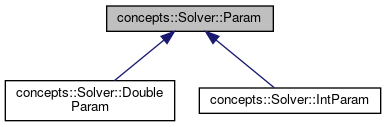
\includegraphics[width=350pt]{classconcepts_1_1_solver_1_1_param__inherit__graph}
\end{center}
\end{figure}
\subsection*{Public Member Functions}
\begin{DoxyCompactItemize}
\item 
virtual \hyperlink{classconcepts_1_1_solver_1_1_param_a9cfb9b36634ad826bf5766306b9823bd}{$\sim$\+Param} ()
\item 
virtual void \hyperlink{classconcepts_1_1_solver_1_1_param_a0c2e4d895747668b01339db9226eceae}{parse} (const char $\ast$arg)=0
\item 
virtual void \hyperlink{classconcepts_1_1_solver_1_1_param_aa525a1a88dd771eaf5d66f35323fbb86}{set} (bool v)=0
\item 
virtual void \hyperlink{classconcepts_1_1_solver_1_1_param_ad3de8144a70e67eeae4278f534e46274}{set} (int v)=0
\item 
virtual void \hyperlink{classconcepts_1_1_solver_1_1_param_a35b7155d8f6db1b3e63e60b883beebcb}{set} (double v)=0
\item 
virtual bool \hyperlink{classconcepts_1_1_solver_1_1_param_aaca8a78f4669d189764e9e654143d705}{get\+Bool} () const =0
\item 
virtual int \hyperlink{classconcepts_1_1_solver_1_1_param_ab849633a029055c00d828df3adb0546e}{get\+Int} () const =0
\item 
virtual double \hyperlink{classconcepts_1_1_solver_1_1_param_a50d288b81da0b77d342e46e75f9b4bfc}{get\+Double} () const =0
\item 
virtual std\+::string \hyperlink{classconcepts_1_1_solver_1_1_param_abcbd9c68852499c7be9ebf6a2d22f4b5}{to\+String} () const =0
\end{DoxyCompactItemize}


\subsection{Constructor \& Destructor Documentation}
\mbox{\Hypertarget{classconcepts_1_1_solver_1_1_param_a9cfb9b36634ad826bf5766306b9823bd}\label{classconcepts_1_1_solver_1_1_param_a9cfb9b36634ad826bf5766306b9823bd}} 
\index{concepts\+::\+Solver\+::\+Param@{concepts\+::\+Solver\+::\+Param}!````~Param@{$\sim$\+Param}}
\index{````~Param@{$\sim$\+Param}!concepts\+::\+Solver\+::\+Param@{concepts\+::\+Solver\+::\+Param}}
\subsubsection{\texorpdfstring{$\sim$\+Param()}{~Param()}}
{\footnotesize\ttfamily virtual concepts\+::\+Solver\+::\+Param\+::$\sim$\+Param (\begin{DoxyParamCaption}{ }\end{DoxyParamCaption})\hspace{0.3cm}{\ttfamily [inline]}, {\ttfamily [virtual]}}



\subsection{Member Function Documentation}
\mbox{\Hypertarget{classconcepts_1_1_solver_1_1_param_aaca8a78f4669d189764e9e654143d705}\label{classconcepts_1_1_solver_1_1_param_aaca8a78f4669d189764e9e654143d705}} 
\index{concepts\+::\+Solver\+::\+Param@{concepts\+::\+Solver\+::\+Param}!get\+Bool@{get\+Bool}}
\index{get\+Bool@{get\+Bool}!concepts\+::\+Solver\+::\+Param@{concepts\+::\+Solver\+::\+Param}}
\subsubsection{\texorpdfstring{get\+Bool()}{getBool()}}
{\footnotesize\ttfamily virtual bool concepts\+::\+Solver\+::\+Param\+::get\+Bool (\begin{DoxyParamCaption}{ }\end{DoxyParamCaption}) const\hspace{0.3cm}{\ttfamily [pure virtual]}}



Implemented in \hyperlink{classconcepts_1_1_solver_1_1_double_param_a59c7fa9b821c071f13d6182d6b525473}{concepts\+::\+Solver\+::\+Double\+Param}, and \hyperlink{classconcepts_1_1_solver_1_1_int_param_aa991108bd194ff4f9cb21230549a74f5}{concepts\+::\+Solver\+::\+Int\+Param}.

\mbox{\Hypertarget{classconcepts_1_1_solver_1_1_param_a50d288b81da0b77d342e46e75f9b4bfc}\label{classconcepts_1_1_solver_1_1_param_a50d288b81da0b77d342e46e75f9b4bfc}} 
\index{concepts\+::\+Solver\+::\+Param@{concepts\+::\+Solver\+::\+Param}!get\+Double@{get\+Double}}
\index{get\+Double@{get\+Double}!concepts\+::\+Solver\+::\+Param@{concepts\+::\+Solver\+::\+Param}}
\subsubsection{\texorpdfstring{get\+Double()}{getDouble()}}
{\footnotesize\ttfamily virtual double concepts\+::\+Solver\+::\+Param\+::get\+Double (\begin{DoxyParamCaption}{ }\end{DoxyParamCaption}) const\hspace{0.3cm}{\ttfamily [pure virtual]}}



Implemented in \hyperlink{classconcepts_1_1_solver_1_1_double_param_a39d5bb1d5b33ef84c8c015b977b438d9}{concepts\+::\+Solver\+::\+Double\+Param}, and \hyperlink{classconcepts_1_1_solver_1_1_int_param_a70b472a5cce3b44e0d9a08f5da70e1a4}{concepts\+::\+Solver\+::\+Int\+Param}.

\mbox{\Hypertarget{classconcepts_1_1_solver_1_1_param_ab849633a029055c00d828df3adb0546e}\label{classconcepts_1_1_solver_1_1_param_ab849633a029055c00d828df3adb0546e}} 
\index{concepts\+::\+Solver\+::\+Param@{concepts\+::\+Solver\+::\+Param}!get\+Int@{get\+Int}}
\index{get\+Int@{get\+Int}!concepts\+::\+Solver\+::\+Param@{concepts\+::\+Solver\+::\+Param}}
\subsubsection{\texorpdfstring{get\+Int()}{getInt()}}
{\footnotesize\ttfamily virtual int concepts\+::\+Solver\+::\+Param\+::get\+Int (\begin{DoxyParamCaption}{ }\end{DoxyParamCaption}) const\hspace{0.3cm}{\ttfamily [pure virtual]}}



Implemented in \hyperlink{classconcepts_1_1_solver_1_1_double_param_a19c83a217a6b73891548850869e9c230}{concepts\+::\+Solver\+::\+Double\+Param}, and \hyperlink{classconcepts_1_1_solver_1_1_int_param_a8ff3d45bcc5fc60750183e61ff61b48e}{concepts\+::\+Solver\+::\+Int\+Param}.

\mbox{\Hypertarget{classconcepts_1_1_solver_1_1_param_a0c2e4d895747668b01339db9226eceae}\label{classconcepts_1_1_solver_1_1_param_a0c2e4d895747668b01339db9226eceae}} 
\index{concepts\+::\+Solver\+::\+Param@{concepts\+::\+Solver\+::\+Param}!parse@{parse}}
\index{parse@{parse}!concepts\+::\+Solver\+::\+Param@{concepts\+::\+Solver\+::\+Param}}
\subsubsection{\texorpdfstring{parse()}{parse()}}
{\footnotesize\ttfamily virtual void concepts\+::\+Solver\+::\+Param\+::parse (\begin{DoxyParamCaption}\item[{const char $\ast$}]{arg }\end{DoxyParamCaption})\hspace{0.3cm}{\ttfamily [pure virtual]}}



Implemented in \hyperlink{classconcepts_1_1_solver_1_1_double_param_a9d9cf1f190f8e7b7c4840f0d44fefa1b}{concepts\+::\+Solver\+::\+Double\+Param}, and \hyperlink{classconcepts_1_1_solver_1_1_int_param_a81c8c88fe73047c6c1b8d5a87d70be24}{concepts\+::\+Solver\+::\+Int\+Param}.

\mbox{\Hypertarget{classconcepts_1_1_solver_1_1_param_aa525a1a88dd771eaf5d66f35323fbb86}\label{classconcepts_1_1_solver_1_1_param_aa525a1a88dd771eaf5d66f35323fbb86}} 
\index{concepts\+::\+Solver\+::\+Param@{concepts\+::\+Solver\+::\+Param}!set@{set}}
\index{set@{set}!concepts\+::\+Solver\+::\+Param@{concepts\+::\+Solver\+::\+Param}}
\subsubsection{\texorpdfstring{set()}{set()}\hspace{0.1cm}{\footnotesize\ttfamily [1/3]}}
{\footnotesize\ttfamily virtual void concepts\+::\+Solver\+::\+Param\+::set (\begin{DoxyParamCaption}\item[{bool}]{v }\end{DoxyParamCaption})\hspace{0.3cm}{\ttfamily [pure virtual]}}



Implemented in \hyperlink{classconcepts_1_1_solver_1_1_double_param_a006e726301f821c96edb00b4ca2ea345}{concepts\+::\+Solver\+::\+Double\+Param}, and \hyperlink{classconcepts_1_1_solver_1_1_int_param_aad1fef920b810b30289a2863d4ab6a52}{concepts\+::\+Solver\+::\+Int\+Param}.

\mbox{\Hypertarget{classconcepts_1_1_solver_1_1_param_ad3de8144a70e67eeae4278f534e46274}\label{classconcepts_1_1_solver_1_1_param_ad3de8144a70e67eeae4278f534e46274}} 
\index{concepts\+::\+Solver\+::\+Param@{concepts\+::\+Solver\+::\+Param}!set@{set}}
\index{set@{set}!concepts\+::\+Solver\+::\+Param@{concepts\+::\+Solver\+::\+Param}}
\subsubsection{\texorpdfstring{set()}{set()}\hspace{0.1cm}{\footnotesize\ttfamily [2/3]}}
{\footnotesize\ttfamily virtual void concepts\+::\+Solver\+::\+Param\+::set (\begin{DoxyParamCaption}\item[{int}]{v }\end{DoxyParamCaption})\hspace{0.3cm}{\ttfamily [pure virtual]}}



Implemented in \hyperlink{classconcepts_1_1_solver_1_1_double_param_a4648d672a792ded79977319d968fd497}{concepts\+::\+Solver\+::\+Double\+Param}, and \hyperlink{classconcepts_1_1_solver_1_1_int_param_aad283b6869373847cf9543e889f9fc91}{concepts\+::\+Solver\+::\+Int\+Param}.

\mbox{\Hypertarget{classconcepts_1_1_solver_1_1_param_a35b7155d8f6db1b3e63e60b883beebcb}\label{classconcepts_1_1_solver_1_1_param_a35b7155d8f6db1b3e63e60b883beebcb}} 
\index{concepts\+::\+Solver\+::\+Param@{concepts\+::\+Solver\+::\+Param}!set@{set}}
\index{set@{set}!concepts\+::\+Solver\+::\+Param@{concepts\+::\+Solver\+::\+Param}}
\subsubsection{\texorpdfstring{set()}{set()}\hspace{0.1cm}{\footnotesize\ttfamily [3/3]}}
{\footnotesize\ttfamily virtual void concepts\+::\+Solver\+::\+Param\+::set (\begin{DoxyParamCaption}\item[{double}]{v }\end{DoxyParamCaption})\hspace{0.3cm}{\ttfamily [pure virtual]}}



Implemented in \hyperlink{classconcepts_1_1_solver_1_1_double_param_a5a27e7e058121b520d71472e8de549db}{concepts\+::\+Solver\+::\+Double\+Param}, and \hyperlink{classconcepts_1_1_solver_1_1_int_param_aa678f7356cd371ac1bc11e86e0109ae7}{concepts\+::\+Solver\+::\+Int\+Param}.

\mbox{\Hypertarget{classconcepts_1_1_solver_1_1_param_abcbd9c68852499c7be9ebf6a2d22f4b5}\label{classconcepts_1_1_solver_1_1_param_abcbd9c68852499c7be9ebf6a2d22f4b5}} 
\index{concepts\+::\+Solver\+::\+Param@{concepts\+::\+Solver\+::\+Param}!to\+String@{to\+String}}
\index{to\+String@{to\+String}!concepts\+::\+Solver\+::\+Param@{concepts\+::\+Solver\+::\+Param}}
\subsubsection{\texorpdfstring{to\+String()}{toString()}}
{\footnotesize\ttfamily virtual std\+::string concepts\+::\+Solver\+::\+Param\+::to\+String (\begin{DoxyParamCaption}{ }\end{DoxyParamCaption}) const\hspace{0.3cm}{\ttfamily [pure virtual]}}



Implemented in \hyperlink{classconcepts_1_1_solver_1_1_double_param_a536f65af0681a1e3af0e101f952f717c}{concepts\+::\+Solver\+::\+Double\+Param}, and \hyperlink{classconcepts_1_1_solver_1_1_int_param_a84740f9d96205d4b7fbc1e011a82e08b}{concepts\+::\+Solver\+::\+Int\+Param}.



The documentation for this class was generated from the following file\+:\begin{DoxyCompactItemize}
\item 
/home/plaiseek/\+Projects/landscape\+\_\+opt\+\_\+cpp/include/solvers/concept/\hyperlink{solver_8hpp}{solver.\+hpp}\end{DoxyCompactItemize}

\hypertarget{classconcepts_1_1_parser}{}\section{concepts\+:\+:Parser$<$ T $>$ Class Template Reference}
\label{classconcepts_1_1_parser}\index{concepts\+::\+Parser$<$ T $>$@{concepts\+::\+Parser$<$ T $>$}}


{\ttfamily \#include $<$parser.\+hpp$>$}

\subsection*{Public Member Functions}
\begin{DoxyCompactItemize}
\item 
\hyperlink{classconcepts_1_1_parser_ab80c529e217209d73ee57a1caf166710}{$\sim$\+Parser} ()
\item 
virtual T $\ast$ \hyperlink{classconcepts_1_1_parser_ac5e6fbf08f6d462695c946647aafb2ce}{parse} (std\+::filesystem\+::path file\+\_\+path)=0
\end{DoxyCompactItemize}
\subsection*{Protected Member Functions}
\begin{DoxyCompactItemize}
\item 
\hyperlink{classconcepts_1_1_parser_a649e088ec83277c61704ed90c4c9f59e}{Parser} ()
\end{DoxyCompactItemize}


\subsection{Constructor \& Destructor Documentation}
\mbox{\Hypertarget{classconcepts_1_1_parser_a649e088ec83277c61704ed90c4c9f59e}\label{classconcepts_1_1_parser_a649e088ec83277c61704ed90c4c9f59e}} 
\index{concepts\+::\+Parser@{concepts\+::\+Parser}!Parser@{Parser}}
\index{Parser@{Parser}!concepts\+::\+Parser@{concepts\+::\+Parser}}
\subsubsection{\texorpdfstring{Parser()}{Parser()}}
{\footnotesize\ttfamily template$<$typename T$>$ \\
\hyperlink{classconcepts_1_1_parser}{concepts\+::\+Parser}$<$ T $>$\+::\hyperlink{classconcepts_1_1_parser}{Parser} (\begin{DoxyParamCaption}{ }\end{DoxyParamCaption})\hspace{0.3cm}{\ttfamily [inline]}, {\ttfamily [protected]}}

\mbox{\Hypertarget{classconcepts_1_1_parser_ab80c529e217209d73ee57a1caf166710}\label{classconcepts_1_1_parser_ab80c529e217209d73ee57a1caf166710}} 
\index{concepts\+::\+Parser@{concepts\+::\+Parser}!````~Parser@{$\sim$\+Parser}}
\index{````~Parser@{$\sim$\+Parser}!concepts\+::\+Parser@{concepts\+::\+Parser}}
\subsubsection{\texorpdfstring{$\sim$\+Parser()}{~Parser()}}
{\footnotesize\ttfamily template$<$typename T$>$ \\
\hyperlink{classconcepts_1_1_parser}{concepts\+::\+Parser}$<$ T $>$\+::$\sim$\hyperlink{classconcepts_1_1_parser}{Parser} (\begin{DoxyParamCaption}{ }\end{DoxyParamCaption})\hspace{0.3cm}{\ttfamily [inline]}}



\subsection{Member Function Documentation}
\mbox{\Hypertarget{classconcepts_1_1_parser_ac5e6fbf08f6d462695c946647aafb2ce}\label{classconcepts_1_1_parser_ac5e6fbf08f6d462695c946647aafb2ce}} 
\index{concepts\+::\+Parser@{concepts\+::\+Parser}!parse@{parse}}
\index{parse@{parse}!concepts\+::\+Parser@{concepts\+::\+Parser}}
\subsubsection{\texorpdfstring{parse()}{parse()}}
{\footnotesize\ttfamily template$<$typename T$>$ \\
virtual T$\ast$ \hyperlink{classconcepts_1_1_parser}{concepts\+::\+Parser}$<$ T $>$\+::parse (\begin{DoxyParamCaption}\item[{std\+::filesystem\+::path}]{file\+\_\+path }\end{DoxyParamCaption})\hspace{0.3cm}{\ttfamily [pure virtual]}}



Implemented in \hyperlink{class_std_landscape_parser_a73c807c756f6f6a90d23d95d91a4e700}{Std\+Landscape\+Parser}, and \hyperlink{class_std_restoration_plan_parser_aa9156823445695123f32e2eb232a3509}{Std\+Restoration\+Plan\+Parser}.



The documentation for this class was generated from the following file\+:\begin{DoxyCompactItemize}
\item 
/home/plaiseek/\+Projects/landscape\+\_\+opt\+\_\+cpp/include/parsers/concept/\hyperlink{parser_8hpp}{parser.\+hpp}\end{DoxyCompactItemize}

\hypertarget{class_solvers_1_1_p_l___e_c_a__2}{}\section{Solvers\+:\+:P\+L\+\_\+\+E\+C\+A\+\_\+2 Class Reference}
\label{class_solvers_1_1_p_l___e_c_a__2}\index{Solvers\+::\+P\+L\+\_\+\+E\+C\+A\+\_\+2@{Solvers\+::\+P\+L\+\_\+\+E\+C\+A\+\_\+2}}


{\ttfamily \#include $<$pl\+\_\+eca\+\_\+2.\+hpp$>$}



Inheritance diagram for Solvers\+:\+:P\+L\+\_\+\+E\+C\+A\+\_\+2\+:\nopagebreak
\begin{figure}[H]
\begin{center}
\leavevmode
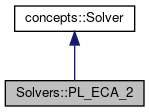
\includegraphics[width=184pt]{class_solvers_1_1_p_l___e_c_a__2__inherit__graph}
\end{center}
\end{figure}


Collaboration diagram for Solvers\+:\+:P\+L\+\_\+\+E\+C\+A\+\_\+2\+:\nopagebreak
\begin{figure}[H]
\begin{center}
\leavevmode
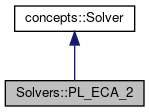
\includegraphics[width=184pt]{class_solvers_1_1_p_l___e_c_a__2__coll__graph}
\end{center}
\end{figure}
\subsection*{Public Member Functions}
\begin{DoxyCompactItemize}
\item 
\hyperlink{class_solvers_1_1_p_l___e_c_a__2_adcc16b55e0d26128fe508bc3f282c29a}{P\+L\+\_\+\+E\+C\+A\+\_\+2} ()
\item 
\hyperlink{class_solvers_1_1_p_l___e_c_a__2}{P\+L\+\_\+\+E\+C\+A\+\_\+2} \& \hyperlink{class_solvers_1_1_p_l___e_c_a__2_a1d868cd61115206cdc692fff35fa584e}{set\+Log\+Level} (int log\+\_\+level)
\item 
\hyperlink{class_solvers_1_1_p_l___e_c_a__2}{P\+L\+\_\+\+E\+C\+A\+\_\+2} \& \hyperlink{class_solvers_1_1_p_l___e_c_a__2_a893f9660cdc4cfd0eab2db5bb7e82407}{set\+Nb\+Threads} (int nb\+\_\+threads)
\item 
\hyperlink{class_solvers_1_1_p_l___e_c_a__2}{P\+L\+\_\+\+E\+C\+A\+\_\+2} \& \hyperlink{class_solvers_1_1_p_l___e_c_a__2_a98ab5e83866c6beeb706ed86cd14afa1}{set\+Relaxed} (bool relaxed)
\item 
\hyperlink{class_solvers_1_1_p_l___e_c_a__2}{P\+L\+\_\+\+E\+C\+A\+\_\+2} \& \hyperlink{class_solvers_1_1_p_l___e_c_a__2_a40ef2df054be492783836af74a3436b3}{set\+Timeout} (int seconds)
\item 
\hyperlink{class_solvers_1_1_p_l___e_c_a__2}{P\+L\+\_\+\+E\+C\+A\+\_\+2} \& \hyperlink{class_solvers_1_1_p_l___e_c_a__2_ae57ac8fbae31047fb0a9d72f7427a661}{set\+Fortest} (int fortest)
\item 
\hyperlink{class_solution}{Solution} $\ast$ \hyperlink{class_solvers_1_1_p_l___e_c_a__2_a07601fa43e0c530e7a66b1532a9e96a6}{solve} (const \hyperlink{class_landscape}{Landscape} \&landscape, const \hyperlink{class_restoration_plan}{Restoration\+Plan} \&options, const double B) const
\item 
const std\+::string \hyperlink{class_solvers_1_1_p_l___e_c_a__2_ab9879a904a2545d929bd2956f23fa1aa}{name} () const
\item 
double \hyperlink{class_solvers_1_1_p_l___e_c_a__2_acc94c4cef3ea294af20215ae2ec77711}{eval} (const \hyperlink{class_landscape}{Landscape} \&landscape, const \hyperlink{class_restoration_plan}{Restoration\+Plan} \&plan, const double B, const \hyperlink{class_solution}{Solution} \&solution) const
\end{DoxyCompactItemize}
\subsection*{Additional Inherited Members}


\subsection{Constructor \& Destructor Documentation}
\mbox{\Hypertarget{class_solvers_1_1_p_l___e_c_a__2_adcc16b55e0d26128fe508bc3f282c29a}\label{class_solvers_1_1_p_l___e_c_a__2_adcc16b55e0d26128fe508bc3f282c29a}} 
\index{Solvers\+::\+P\+L\+\_\+\+E\+C\+A\+\_\+2@{Solvers\+::\+P\+L\+\_\+\+E\+C\+A\+\_\+2}!P\+L\+\_\+\+E\+C\+A\+\_\+2@{P\+L\+\_\+\+E\+C\+A\+\_\+2}}
\index{P\+L\+\_\+\+E\+C\+A\+\_\+2@{P\+L\+\_\+\+E\+C\+A\+\_\+2}!Solvers\+::\+P\+L\+\_\+\+E\+C\+A\+\_\+2@{Solvers\+::\+P\+L\+\_\+\+E\+C\+A\+\_\+2}}
\subsubsection{\texorpdfstring{P\+L\+\_\+\+E\+C\+A\+\_\+2()}{PL\_ECA\_2()}}
{\footnotesize\ttfamily Solvers\+::\+P\+L\+\_\+\+E\+C\+A\+\_\+2\+::\+P\+L\+\_\+\+E\+C\+A\+\_\+2 (\begin{DoxyParamCaption}{ }\end{DoxyParamCaption})\hspace{0.3cm}{\ttfamily [inline]}}



\subsection{Member Function Documentation}
\mbox{\Hypertarget{class_solvers_1_1_p_l___e_c_a__2_acc94c4cef3ea294af20215ae2ec77711}\label{class_solvers_1_1_p_l___e_c_a__2_acc94c4cef3ea294af20215ae2ec77711}} 
\index{Solvers\+::\+P\+L\+\_\+\+E\+C\+A\+\_\+2@{Solvers\+::\+P\+L\+\_\+\+E\+C\+A\+\_\+2}!eval@{eval}}
\index{eval@{eval}!Solvers\+::\+P\+L\+\_\+\+E\+C\+A\+\_\+2@{Solvers\+::\+P\+L\+\_\+\+E\+C\+A\+\_\+2}}
\subsubsection{\texorpdfstring{eval()}{eval()}}
{\footnotesize\ttfamily double Solvers\+::\+P\+L\+\_\+\+E\+C\+A\+\_\+2\+::eval (\begin{DoxyParamCaption}\item[{const \hyperlink{class_landscape}{Landscape} \&}]{landscape,  }\item[{const \hyperlink{class_restoration_plan}{Restoration\+Plan} \&}]{plan,  }\item[{const double}]{B,  }\item[{const \hyperlink{class_solution}{Solution} \&}]{solution }\end{DoxyParamCaption}) const}

\mbox{\Hypertarget{class_solvers_1_1_p_l___e_c_a__2_ab9879a904a2545d929bd2956f23fa1aa}\label{class_solvers_1_1_p_l___e_c_a__2_ab9879a904a2545d929bd2956f23fa1aa}} 
\index{Solvers\+::\+P\+L\+\_\+\+E\+C\+A\+\_\+2@{Solvers\+::\+P\+L\+\_\+\+E\+C\+A\+\_\+2}!name@{name}}
\index{name@{name}!Solvers\+::\+P\+L\+\_\+\+E\+C\+A\+\_\+2@{Solvers\+::\+P\+L\+\_\+\+E\+C\+A\+\_\+2}}
\subsubsection{\texorpdfstring{name()}{name()}}
{\footnotesize\ttfamily const std\+::string Solvers\+::\+P\+L\+\_\+\+E\+C\+A\+\_\+2\+::name (\begin{DoxyParamCaption}{ }\end{DoxyParamCaption}) const\hspace{0.3cm}{\ttfamily [inline]}, {\ttfamily [virtual]}}



Implements \hyperlink{classconcepts_1_1_solver_ab995568318a506446228f45cab2fcce7}{concepts\+::\+Solver}.

\mbox{\Hypertarget{class_solvers_1_1_p_l___e_c_a__2_ae57ac8fbae31047fb0a9d72f7427a661}\label{class_solvers_1_1_p_l___e_c_a__2_ae57ac8fbae31047fb0a9d72f7427a661}} 
\index{Solvers\+::\+P\+L\+\_\+\+E\+C\+A\+\_\+2@{Solvers\+::\+P\+L\+\_\+\+E\+C\+A\+\_\+2}!set\+Fortest@{set\+Fortest}}
\index{set\+Fortest@{set\+Fortest}!Solvers\+::\+P\+L\+\_\+\+E\+C\+A\+\_\+2@{Solvers\+::\+P\+L\+\_\+\+E\+C\+A\+\_\+2}}
\subsubsection{\texorpdfstring{set\+Fortest()}{setFortest()}}
{\footnotesize\ttfamily \hyperlink{class_solvers_1_1_p_l___e_c_a__2}{P\+L\+\_\+\+E\+C\+A\+\_\+2}\& Solvers\+::\+P\+L\+\_\+\+E\+C\+A\+\_\+2\+::set\+Fortest (\begin{DoxyParamCaption}\item[{int}]{fortest }\end{DoxyParamCaption})\hspace{0.3cm}{\ttfamily [inline]}}

\mbox{\Hypertarget{class_solvers_1_1_p_l___e_c_a__2_a1d868cd61115206cdc692fff35fa584e}\label{class_solvers_1_1_p_l___e_c_a__2_a1d868cd61115206cdc692fff35fa584e}} 
\index{Solvers\+::\+P\+L\+\_\+\+E\+C\+A\+\_\+2@{Solvers\+::\+P\+L\+\_\+\+E\+C\+A\+\_\+2}!set\+Log\+Level@{set\+Log\+Level}}
\index{set\+Log\+Level@{set\+Log\+Level}!Solvers\+::\+P\+L\+\_\+\+E\+C\+A\+\_\+2@{Solvers\+::\+P\+L\+\_\+\+E\+C\+A\+\_\+2}}
\subsubsection{\texorpdfstring{set\+Log\+Level()}{setLogLevel()}}
{\footnotesize\ttfamily \hyperlink{class_solvers_1_1_p_l___e_c_a__2}{P\+L\+\_\+\+E\+C\+A\+\_\+2}\& Solvers\+::\+P\+L\+\_\+\+E\+C\+A\+\_\+2\+::set\+Log\+Level (\begin{DoxyParamCaption}\item[{int}]{log\+\_\+level }\end{DoxyParamCaption})\hspace{0.3cm}{\ttfamily [inline]}}

\mbox{\Hypertarget{class_solvers_1_1_p_l___e_c_a__2_a893f9660cdc4cfd0eab2db5bb7e82407}\label{class_solvers_1_1_p_l___e_c_a__2_a893f9660cdc4cfd0eab2db5bb7e82407}} 
\index{Solvers\+::\+P\+L\+\_\+\+E\+C\+A\+\_\+2@{Solvers\+::\+P\+L\+\_\+\+E\+C\+A\+\_\+2}!set\+Nb\+Threads@{set\+Nb\+Threads}}
\index{set\+Nb\+Threads@{set\+Nb\+Threads}!Solvers\+::\+P\+L\+\_\+\+E\+C\+A\+\_\+2@{Solvers\+::\+P\+L\+\_\+\+E\+C\+A\+\_\+2}}
\subsubsection{\texorpdfstring{set\+Nb\+Threads()}{setNbThreads()}}
{\footnotesize\ttfamily \hyperlink{class_solvers_1_1_p_l___e_c_a__2}{P\+L\+\_\+\+E\+C\+A\+\_\+2}\& Solvers\+::\+P\+L\+\_\+\+E\+C\+A\+\_\+2\+::set\+Nb\+Threads (\begin{DoxyParamCaption}\item[{int}]{nb\+\_\+threads }\end{DoxyParamCaption})\hspace{0.3cm}{\ttfamily [inline]}}

\mbox{\Hypertarget{class_solvers_1_1_p_l___e_c_a__2_a98ab5e83866c6beeb706ed86cd14afa1}\label{class_solvers_1_1_p_l___e_c_a__2_a98ab5e83866c6beeb706ed86cd14afa1}} 
\index{Solvers\+::\+P\+L\+\_\+\+E\+C\+A\+\_\+2@{Solvers\+::\+P\+L\+\_\+\+E\+C\+A\+\_\+2}!set\+Relaxed@{set\+Relaxed}}
\index{set\+Relaxed@{set\+Relaxed}!Solvers\+::\+P\+L\+\_\+\+E\+C\+A\+\_\+2@{Solvers\+::\+P\+L\+\_\+\+E\+C\+A\+\_\+2}}
\subsubsection{\texorpdfstring{set\+Relaxed()}{setRelaxed()}}
{\footnotesize\ttfamily \hyperlink{class_solvers_1_1_p_l___e_c_a__2}{P\+L\+\_\+\+E\+C\+A\+\_\+2}\& Solvers\+::\+P\+L\+\_\+\+E\+C\+A\+\_\+2\+::set\+Relaxed (\begin{DoxyParamCaption}\item[{bool}]{relaxed }\end{DoxyParamCaption})\hspace{0.3cm}{\ttfamily [inline]}}

\mbox{\Hypertarget{class_solvers_1_1_p_l___e_c_a__2_a40ef2df054be492783836af74a3436b3}\label{class_solvers_1_1_p_l___e_c_a__2_a40ef2df054be492783836af74a3436b3}} 
\index{Solvers\+::\+P\+L\+\_\+\+E\+C\+A\+\_\+2@{Solvers\+::\+P\+L\+\_\+\+E\+C\+A\+\_\+2}!set\+Timeout@{set\+Timeout}}
\index{set\+Timeout@{set\+Timeout}!Solvers\+::\+P\+L\+\_\+\+E\+C\+A\+\_\+2@{Solvers\+::\+P\+L\+\_\+\+E\+C\+A\+\_\+2}}
\subsubsection{\texorpdfstring{set\+Timeout()}{setTimeout()}}
{\footnotesize\ttfamily \hyperlink{class_solvers_1_1_p_l___e_c_a__2}{P\+L\+\_\+\+E\+C\+A\+\_\+2}\& Solvers\+::\+P\+L\+\_\+\+E\+C\+A\+\_\+2\+::set\+Timeout (\begin{DoxyParamCaption}\item[{int}]{seconds }\end{DoxyParamCaption})\hspace{0.3cm}{\ttfamily [inline]}}

\mbox{\Hypertarget{class_solvers_1_1_p_l___e_c_a__2_a07601fa43e0c530e7a66b1532a9e96a6}\label{class_solvers_1_1_p_l___e_c_a__2_a07601fa43e0c530e7a66b1532a9e96a6}} 
\index{Solvers\+::\+P\+L\+\_\+\+E\+C\+A\+\_\+2@{Solvers\+::\+P\+L\+\_\+\+E\+C\+A\+\_\+2}!solve@{solve}}
\index{solve@{solve}!Solvers\+::\+P\+L\+\_\+\+E\+C\+A\+\_\+2@{Solvers\+::\+P\+L\+\_\+\+E\+C\+A\+\_\+2}}
\subsubsection{\texorpdfstring{solve()}{solve()}}
{\footnotesize\ttfamily \hyperlink{class_solution}{Solution} $\ast$ Solvers\+::\+P\+L\+\_\+\+E\+C\+A\+\_\+2\+::solve (\begin{DoxyParamCaption}\item[{const \hyperlink{class_landscape}{Landscape} \&}]{landscape,  }\item[{const \hyperlink{class_restoration_plan}{Restoration\+Plan} \&}]{options,  }\item[{const double}]{B }\end{DoxyParamCaption}) const\hspace{0.3cm}{\ttfamily [virtual]}}



Implements \hyperlink{classconcepts_1_1_solver_af323ad29df1e7b87facd7dc007568c80}{concepts\+::\+Solver}.



The documentation for this class was generated from the following files\+:\begin{DoxyCompactItemize}
\item 
/home/plaiseek/\+Projects/landscape\+\_\+opt\+\_\+cpp/include/solvers/\hyperlink{pl__eca__2_8hpp}{pl\+\_\+eca\+\_\+2.\+hpp}\item 
/home/plaiseek/\+Projects/landscape\+\_\+opt\+\_\+cpp/src/solvers/\hyperlink{pl__eca__2_8cpp}{pl\+\_\+eca\+\_\+2.\+cpp}\end{DoxyCompactItemize}

\hypertarget{class_solvers_1_1_p_l___e_c_a__3}{}\section{Solvers\+:\+:P\+L\+\_\+\+E\+C\+A\+\_\+3 Class Reference}
\label{class_solvers_1_1_p_l___e_c_a__3}\index{Solvers\+::\+P\+L\+\_\+\+E\+C\+A\+\_\+3@{Solvers\+::\+P\+L\+\_\+\+E\+C\+A\+\_\+3}}


{\ttfamily \#include $<$pl\+\_\+eca\+\_\+3.\+hpp$>$}



Inheritance diagram for Solvers\+:\+:P\+L\+\_\+\+E\+C\+A\+\_\+3\+:\nopagebreak
\begin{figure}[H]
\begin{center}
\leavevmode
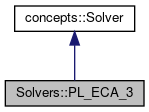
\includegraphics[width=184pt]{class_solvers_1_1_p_l___e_c_a__3__inherit__graph}
\end{center}
\end{figure}


Collaboration diagram for Solvers\+:\+:P\+L\+\_\+\+E\+C\+A\+\_\+3\+:\nopagebreak
\begin{figure}[H]
\begin{center}
\leavevmode
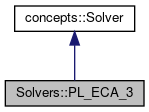
\includegraphics[width=184pt]{class_solvers_1_1_p_l___e_c_a__3__coll__graph}
\end{center}
\end{figure}
\subsection*{Public Member Functions}
\begin{DoxyCompactItemize}
\item 
\hyperlink{class_solvers_1_1_p_l___e_c_a__3_a9af5b2a3a8f0df9de16a23781d56066a}{P\+L\+\_\+\+E\+C\+A\+\_\+3} ()
\item 
\hyperlink{class_solvers_1_1_p_l___e_c_a__3}{P\+L\+\_\+\+E\+C\+A\+\_\+3} \& \hyperlink{class_solvers_1_1_p_l___e_c_a__3_a009037ee169b9b0f372a85925274eaba}{set\+Log\+Level} (int log\+\_\+level)
\item 
\hyperlink{class_solvers_1_1_p_l___e_c_a__3}{P\+L\+\_\+\+E\+C\+A\+\_\+3} \& \hyperlink{class_solvers_1_1_p_l___e_c_a__3_a112c187ccdabdc24bb7f9bf670ece7e1}{set\+Nb\+Threads} (int nb\+\_\+threads)
\item 
\hyperlink{class_solvers_1_1_p_l___e_c_a__3}{P\+L\+\_\+\+E\+C\+A\+\_\+3} \& \hyperlink{class_solvers_1_1_p_l___e_c_a__3_af7951a4d24d7d85d2c0dc640fb436d41}{set\+Relaxed} (bool relaxed)
\item 
\hyperlink{class_solvers_1_1_p_l___e_c_a__3}{P\+L\+\_\+\+E\+C\+A\+\_\+3} \& \hyperlink{class_solvers_1_1_p_l___e_c_a__3_a3f39771900d4abb806836b08373c005c}{set\+Timeout} (int seconds)
\item 
\hyperlink{class_solvers_1_1_p_l___e_c_a__3}{P\+L\+\_\+\+E\+C\+A\+\_\+3} \& \hyperlink{class_solvers_1_1_p_l___e_c_a__3_ab4011be3f89d3c26a32486f769365434}{set\+Fortest} (int fortest)
\item 
\hyperlink{class_solution}{Solution} $\ast$ \hyperlink{class_solvers_1_1_p_l___e_c_a__3_ae296efd0061d2fbf478732bc9c280202}{solve} (const \hyperlink{class_landscape}{Landscape} \&landscape, const \hyperlink{class_restoration_plan}{Restoration\+Plan} \&plan, const double B) const
\item 
const std\+::string \hyperlink{class_solvers_1_1_p_l___e_c_a__3_ac265db86ca64eb34ba5370e905686a21}{name} () const
\item 
double \hyperlink{class_solvers_1_1_p_l___e_c_a__3_ae18471edc442194d0e8b786c3eb35f90}{eval} (const \hyperlink{class_landscape}{Landscape} \&landscape, const \hyperlink{class_restoration_plan}{Restoration\+Plan} \&plan, const double B, const \hyperlink{class_solution}{Solution} \&solution) const
\end{DoxyCompactItemize}
\subsection*{Additional Inherited Members}


\subsection{Constructor \& Destructor Documentation}
\mbox{\Hypertarget{class_solvers_1_1_p_l___e_c_a__3_a9af5b2a3a8f0df9de16a23781d56066a}\label{class_solvers_1_1_p_l___e_c_a__3_a9af5b2a3a8f0df9de16a23781d56066a}} 
\index{Solvers\+::\+P\+L\+\_\+\+E\+C\+A\+\_\+3@{Solvers\+::\+P\+L\+\_\+\+E\+C\+A\+\_\+3}!P\+L\+\_\+\+E\+C\+A\+\_\+3@{P\+L\+\_\+\+E\+C\+A\+\_\+3}}
\index{P\+L\+\_\+\+E\+C\+A\+\_\+3@{P\+L\+\_\+\+E\+C\+A\+\_\+3}!Solvers\+::\+P\+L\+\_\+\+E\+C\+A\+\_\+3@{Solvers\+::\+P\+L\+\_\+\+E\+C\+A\+\_\+3}}
\subsubsection{\texorpdfstring{P\+L\+\_\+\+E\+C\+A\+\_\+3()}{PL\_ECA\_3()}}
{\footnotesize\ttfamily Solvers\+::\+P\+L\+\_\+\+E\+C\+A\+\_\+3\+::\+P\+L\+\_\+\+E\+C\+A\+\_\+3 (\begin{DoxyParamCaption}{ }\end{DoxyParamCaption})\hspace{0.3cm}{\ttfamily [inline]}}



\subsection{Member Function Documentation}
\mbox{\Hypertarget{class_solvers_1_1_p_l___e_c_a__3_ae18471edc442194d0e8b786c3eb35f90}\label{class_solvers_1_1_p_l___e_c_a__3_ae18471edc442194d0e8b786c3eb35f90}} 
\index{Solvers\+::\+P\+L\+\_\+\+E\+C\+A\+\_\+3@{Solvers\+::\+P\+L\+\_\+\+E\+C\+A\+\_\+3}!eval@{eval}}
\index{eval@{eval}!Solvers\+::\+P\+L\+\_\+\+E\+C\+A\+\_\+3@{Solvers\+::\+P\+L\+\_\+\+E\+C\+A\+\_\+3}}
\subsubsection{\texorpdfstring{eval()}{eval()}}
{\footnotesize\ttfamily double Solvers\+::\+P\+L\+\_\+\+E\+C\+A\+\_\+3\+::eval (\begin{DoxyParamCaption}\item[{const \hyperlink{class_landscape}{Landscape} \&}]{landscape,  }\item[{const \hyperlink{class_restoration_plan}{Restoration\+Plan} \&}]{plan,  }\item[{const double}]{B,  }\item[{const \hyperlink{class_solution}{Solution} \&}]{solution }\end{DoxyParamCaption}) const}

\mbox{\Hypertarget{class_solvers_1_1_p_l___e_c_a__3_ac265db86ca64eb34ba5370e905686a21}\label{class_solvers_1_1_p_l___e_c_a__3_ac265db86ca64eb34ba5370e905686a21}} 
\index{Solvers\+::\+P\+L\+\_\+\+E\+C\+A\+\_\+3@{Solvers\+::\+P\+L\+\_\+\+E\+C\+A\+\_\+3}!name@{name}}
\index{name@{name}!Solvers\+::\+P\+L\+\_\+\+E\+C\+A\+\_\+3@{Solvers\+::\+P\+L\+\_\+\+E\+C\+A\+\_\+3}}
\subsubsection{\texorpdfstring{name()}{name()}}
{\footnotesize\ttfamily const std\+::string Solvers\+::\+P\+L\+\_\+\+E\+C\+A\+\_\+3\+::name (\begin{DoxyParamCaption}{ }\end{DoxyParamCaption}) const\hspace{0.3cm}{\ttfamily [inline]}, {\ttfamily [virtual]}}



Implements \hyperlink{classconcepts_1_1_solver_ab995568318a506446228f45cab2fcce7}{concepts\+::\+Solver}.

\mbox{\Hypertarget{class_solvers_1_1_p_l___e_c_a__3_ab4011be3f89d3c26a32486f769365434}\label{class_solvers_1_1_p_l___e_c_a__3_ab4011be3f89d3c26a32486f769365434}} 
\index{Solvers\+::\+P\+L\+\_\+\+E\+C\+A\+\_\+3@{Solvers\+::\+P\+L\+\_\+\+E\+C\+A\+\_\+3}!set\+Fortest@{set\+Fortest}}
\index{set\+Fortest@{set\+Fortest}!Solvers\+::\+P\+L\+\_\+\+E\+C\+A\+\_\+3@{Solvers\+::\+P\+L\+\_\+\+E\+C\+A\+\_\+3}}
\subsubsection{\texorpdfstring{set\+Fortest()}{setFortest()}}
{\footnotesize\ttfamily \hyperlink{class_solvers_1_1_p_l___e_c_a__3}{P\+L\+\_\+\+E\+C\+A\+\_\+3}\& Solvers\+::\+P\+L\+\_\+\+E\+C\+A\+\_\+3\+::set\+Fortest (\begin{DoxyParamCaption}\item[{int}]{fortest }\end{DoxyParamCaption})\hspace{0.3cm}{\ttfamily [inline]}}

\mbox{\Hypertarget{class_solvers_1_1_p_l___e_c_a__3_a009037ee169b9b0f372a85925274eaba}\label{class_solvers_1_1_p_l___e_c_a__3_a009037ee169b9b0f372a85925274eaba}} 
\index{Solvers\+::\+P\+L\+\_\+\+E\+C\+A\+\_\+3@{Solvers\+::\+P\+L\+\_\+\+E\+C\+A\+\_\+3}!set\+Log\+Level@{set\+Log\+Level}}
\index{set\+Log\+Level@{set\+Log\+Level}!Solvers\+::\+P\+L\+\_\+\+E\+C\+A\+\_\+3@{Solvers\+::\+P\+L\+\_\+\+E\+C\+A\+\_\+3}}
\subsubsection{\texorpdfstring{set\+Log\+Level()}{setLogLevel()}}
{\footnotesize\ttfamily \hyperlink{class_solvers_1_1_p_l___e_c_a__3}{P\+L\+\_\+\+E\+C\+A\+\_\+3}\& Solvers\+::\+P\+L\+\_\+\+E\+C\+A\+\_\+3\+::set\+Log\+Level (\begin{DoxyParamCaption}\item[{int}]{log\+\_\+level }\end{DoxyParamCaption})\hspace{0.3cm}{\ttfamily [inline]}}

\mbox{\Hypertarget{class_solvers_1_1_p_l___e_c_a__3_a112c187ccdabdc24bb7f9bf670ece7e1}\label{class_solvers_1_1_p_l___e_c_a__3_a112c187ccdabdc24bb7f9bf670ece7e1}} 
\index{Solvers\+::\+P\+L\+\_\+\+E\+C\+A\+\_\+3@{Solvers\+::\+P\+L\+\_\+\+E\+C\+A\+\_\+3}!set\+Nb\+Threads@{set\+Nb\+Threads}}
\index{set\+Nb\+Threads@{set\+Nb\+Threads}!Solvers\+::\+P\+L\+\_\+\+E\+C\+A\+\_\+3@{Solvers\+::\+P\+L\+\_\+\+E\+C\+A\+\_\+3}}
\subsubsection{\texorpdfstring{set\+Nb\+Threads()}{setNbThreads()}}
{\footnotesize\ttfamily \hyperlink{class_solvers_1_1_p_l___e_c_a__3}{P\+L\+\_\+\+E\+C\+A\+\_\+3}\& Solvers\+::\+P\+L\+\_\+\+E\+C\+A\+\_\+3\+::set\+Nb\+Threads (\begin{DoxyParamCaption}\item[{int}]{nb\+\_\+threads }\end{DoxyParamCaption})\hspace{0.3cm}{\ttfamily [inline]}}

\mbox{\Hypertarget{class_solvers_1_1_p_l___e_c_a__3_af7951a4d24d7d85d2c0dc640fb436d41}\label{class_solvers_1_1_p_l___e_c_a__3_af7951a4d24d7d85d2c0dc640fb436d41}} 
\index{Solvers\+::\+P\+L\+\_\+\+E\+C\+A\+\_\+3@{Solvers\+::\+P\+L\+\_\+\+E\+C\+A\+\_\+3}!set\+Relaxed@{set\+Relaxed}}
\index{set\+Relaxed@{set\+Relaxed}!Solvers\+::\+P\+L\+\_\+\+E\+C\+A\+\_\+3@{Solvers\+::\+P\+L\+\_\+\+E\+C\+A\+\_\+3}}
\subsubsection{\texorpdfstring{set\+Relaxed()}{setRelaxed()}}
{\footnotesize\ttfamily \hyperlink{class_solvers_1_1_p_l___e_c_a__3}{P\+L\+\_\+\+E\+C\+A\+\_\+3}\& Solvers\+::\+P\+L\+\_\+\+E\+C\+A\+\_\+3\+::set\+Relaxed (\begin{DoxyParamCaption}\item[{bool}]{relaxed }\end{DoxyParamCaption})\hspace{0.3cm}{\ttfamily [inline]}}

\mbox{\Hypertarget{class_solvers_1_1_p_l___e_c_a__3_a3f39771900d4abb806836b08373c005c}\label{class_solvers_1_1_p_l___e_c_a__3_a3f39771900d4abb806836b08373c005c}} 
\index{Solvers\+::\+P\+L\+\_\+\+E\+C\+A\+\_\+3@{Solvers\+::\+P\+L\+\_\+\+E\+C\+A\+\_\+3}!set\+Timeout@{set\+Timeout}}
\index{set\+Timeout@{set\+Timeout}!Solvers\+::\+P\+L\+\_\+\+E\+C\+A\+\_\+3@{Solvers\+::\+P\+L\+\_\+\+E\+C\+A\+\_\+3}}
\subsubsection{\texorpdfstring{set\+Timeout()}{setTimeout()}}
{\footnotesize\ttfamily \hyperlink{class_solvers_1_1_p_l___e_c_a__3}{P\+L\+\_\+\+E\+C\+A\+\_\+3}\& Solvers\+::\+P\+L\+\_\+\+E\+C\+A\+\_\+3\+::set\+Timeout (\begin{DoxyParamCaption}\item[{int}]{seconds }\end{DoxyParamCaption})\hspace{0.3cm}{\ttfamily [inline]}}

\mbox{\Hypertarget{class_solvers_1_1_p_l___e_c_a__3_ae296efd0061d2fbf478732bc9c280202}\label{class_solvers_1_1_p_l___e_c_a__3_ae296efd0061d2fbf478732bc9c280202}} 
\index{Solvers\+::\+P\+L\+\_\+\+E\+C\+A\+\_\+3@{Solvers\+::\+P\+L\+\_\+\+E\+C\+A\+\_\+3}!solve@{solve}}
\index{solve@{solve}!Solvers\+::\+P\+L\+\_\+\+E\+C\+A\+\_\+3@{Solvers\+::\+P\+L\+\_\+\+E\+C\+A\+\_\+3}}
\subsubsection{\texorpdfstring{solve()}{solve()}}
{\footnotesize\ttfamily \hyperlink{class_solution}{Solution} $\ast$ Solvers\+::\+P\+L\+\_\+\+E\+C\+A\+\_\+3\+::solve (\begin{DoxyParamCaption}\item[{const \hyperlink{class_landscape}{Landscape} \&}]{landscape,  }\item[{const \hyperlink{class_restoration_plan}{Restoration\+Plan} \&}]{plan,  }\item[{const double}]{B }\end{DoxyParamCaption}) const\hspace{0.3cm}{\ttfamily [virtual]}}



Implements \hyperlink{classconcepts_1_1_solver_af323ad29df1e7b87facd7dc007568c80}{concepts\+::\+Solver}.



The documentation for this class was generated from the following files\+:\begin{DoxyCompactItemize}
\item 
/home/plaiseek/\+Projects/landscape\+\_\+opt\+\_\+cpp/include/solvers/\hyperlink{pl__eca__3_8hpp}{pl\+\_\+eca\+\_\+3.\+hpp}\item 
/home/plaiseek/\+Projects/landscape\+\_\+opt\+\_\+cpp/src/solvers/\hyperlink{pl__eca__3_8cpp}{pl\+\_\+eca\+\_\+3.\+cpp}\end{DoxyCompactItemize}

\hypertarget{class_p_l___e_c_a___solver}{}\section{P\+L\+\_\+\+E\+C\+A\+\_\+\+Solver Class Reference}
\label{class_p_l___e_c_a___solver}\index{P\+L\+\_\+\+E\+C\+A\+\_\+\+Solver@{P\+L\+\_\+\+E\+C\+A\+\_\+\+Solver}}


{\ttfamily \#include $<$pl\+\_\+eca.\+hpp$>$}



Inheritance diagram for P\+L\+\_\+\+E\+C\+A\+\_\+\+Solver\+:\nopagebreak
\begin{figure}[H]
\begin{center}
\leavevmode
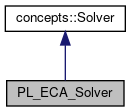
\includegraphics[width=170pt]{class_p_l___e_c_a___solver__inherit__graph}
\end{center}
\end{figure}


Collaboration diagram for P\+L\+\_\+\+E\+C\+A\+\_\+\+Solver\+:\nopagebreak
\begin{figure}[H]
\begin{center}
\leavevmode
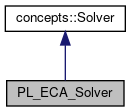
\includegraphics[width=170pt]{class_p_l___e_c_a___solver__coll__graph}
\end{center}
\end{figure}
\subsection*{Public Member Functions}
\begin{DoxyCompactItemize}
\item 
\hyperlink{class_p_l___e_c_a___solver_a2ceebca2d22969b3c1042b79e37ce903}{P\+L\+\_\+\+E\+C\+A\+\_\+\+Solver} ()
\item 
\hyperlink{class_p_l___e_c_a___solver}{P\+L\+\_\+\+E\+C\+A\+\_\+\+Solver} \& \hyperlink{class_p_l___e_c_a___solver_af6b396a9f4d322578f69ad923dbdfc81}{set\+Log\+Level} (int log\+\_\+level)
\item 
\hyperlink{class_p_l___e_c_a___solver}{P\+L\+\_\+\+E\+C\+A\+\_\+\+Solver} \& \hyperlink{class_p_l___e_c_a___solver_a3e0926b81d114ad8754993fe9be92122}{set\+Nb\+Threads} (int nb\+\_\+threads)
\item 
\hyperlink{class_p_l___e_c_a___solver}{P\+L\+\_\+\+E\+C\+A\+\_\+\+Solver} \& \hyperlink{class_p_l___e_c_a___solver_a8da17e87b79839cf35bfaa7a32dca1fd}{set\+Piecewise\+Number} (int g)
\item 
\hyperlink{class_p_l___e_c_a___solver}{P\+L\+\_\+\+E\+C\+A\+\_\+\+Solver} \& \hyperlink{class_p_l___e_c_a___solver_aa08191661fd734646fa916959cac5728}{set\+Pair\+Thresold} (double st\+\_\+thresold)
\item 
\hyperlink{class_p_l___e_c_a___solver}{P\+L\+\_\+\+E\+C\+A\+\_\+\+Solver} \& \hyperlink{class_p_l___e_c_a___solver_ac6c0a8cdb448c759ab706bac5eb857ba}{set\+Relaxed} (bool relaxed)
\item 
\hyperlink{class_p_l___e_c_a___solver}{P\+L\+\_\+\+E\+C\+A\+\_\+\+Solver} \& \hyperlink{class_p_l___e_c_a___solver_a17ca21ad3dd7336e51daddb1ca587389}{set\+Timeout} (int seconds)
\item 
\hyperlink{class_solution}{Solution} $\ast$ \hyperlink{class_p_l___e_c_a___solver_a7fe728bb23be76b4aa51e669b73ee10d}{solve} (const \hyperlink{class_landscape}{Landscape} \&landscape, const \hyperlink{class_restoration_plan}{Restoration\+Plan} \&plan, const double B) const
\item 
const std\+::string \hyperlink{class_p_l___e_c_a___solver_a4cbbcbfd62d91dacb448470456ac57c7}{name} () const
\end{DoxyCompactItemize}
\subsection*{Additional Inherited Members}


\subsection{Constructor \& Destructor Documentation}
\mbox{\Hypertarget{class_p_l___e_c_a___solver_a2ceebca2d22969b3c1042b79e37ce903}\label{class_p_l___e_c_a___solver_a2ceebca2d22969b3c1042b79e37ce903}} 
\index{P\+L\+\_\+\+E\+C\+A\+\_\+\+Solver@{P\+L\+\_\+\+E\+C\+A\+\_\+\+Solver}!P\+L\+\_\+\+E\+C\+A\+\_\+\+Solver@{P\+L\+\_\+\+E\+C\+A\+\_\+\+Solver}}
\index{P\+L\+\_\+\+E\+C\+A\+\_\+\+Solver@{P\+L\+\_\+\+E\+C\+A\+\_\+\+Solver}!P\+L\+\_\+\+E\+C\+A\+\_\+\+Solver@{P\+L\+\_\+\+E\+C\+A\+\_\+\+Solver}}
\subsubsection{\texorpdfstring{P\+L\+\_\+\+E\+C\+A\+\_\+\+Solver()}{PL\_ECA\_Solver()}}
{\footnotesize\ttfamily P\+L\+\_\+\+E\+C\+A\+\_\+\+Solver\+::\+P\+L\+\_\+\+E\+C\+A\+\_\+\+Solver (\begin{DoxyParamCaption}{ }\end{DoxyParamCaption})\hspace{0.3cm}{\ttfamily [inline]}}



\subsection{Member Function Documentation}
\mbox{\Hypertarget{class_p_l___e_c_a___solver_a4cbbcbfd62d91dacb448470456ac57c7}\label{class_p_l___e_c_a___solver_a4cbbcbfd62d91dacb448470456ac57c7}} 
\index{P\+L\+\_\+\+E\+C\+A\+\_\+\+Solver@{P\+L\+\_\+\+E\+C\+A\+\_\+\+Solver}!name@{name}}
\index{name@{name}!P\+L\+\_\+\+E\+C\+A\+\_\+\+Solver@{P\+L\+\_\+\+E\+C\+A\+\_\+\+Solver}}
\subsubsection{\texorpdfstring{name()}{name()}}
{\footnotesize\ttfamily const std\+::string P\+L\+\_\+\+E\+C\+A\+\_\+\+Solver\+::name (\begin{DoxyParamCaption}{ }\end{DoxyParamCaption}) const\hspace{0.3cm}{\ttfamily [inline]}, {\ttfamily [virtual]}}



Implements \hyperlink{classconcepts_1_1_solver_ab995568318a506446228f45cab2fcce7}{concepts\+::\+Solver}.

\mbox{\Hypertarget{class_p_l___e_c_a___solver_af6b396a9f4d322578f69ad923dbdfc81}\label{class_p_l___e_c_a___solver_af6b396a9f4d322578f69ad923dbdfc81}} 
\index{P\+L\+\_\+\+E\+C\+A\+\_\+\+Solver@{P\+L\+\_\+\+E\+C\+A\+\_\+\+Solver}!set\+Log\+Level@{set\+Log\+Level}}
\index{set\+Log\+Level@{set\+Log\+Level}!P\+L\+\_\+\+E\+C\+A\+\_\+\+Solver@{P\+L\+\_\+\+E\+C\+A\+\_\+\+Solver}}
\subsubsection{\texorpdfstring{set\+Log\+Level()}{setLogLevel()}}
{\footnotesize\ttfamily \hyperlink{class_p_l___e_c_a___solver}{P\+L\+\_\+\+E\+C\+A\+\_\+\+Solver}\& P\+L\+\_\+\+E\+C\+A\+\_\+\+Solver\+::set\+Log\+Level (\begin{DoxyParamCaption}\item[{int}]{log\+\_\+level }\end{DoxyParamCaption})\hspace{0.3cm}{\ttfamily [inline]}}

\mbox{\Hypertarget{class_p_l___e_c_a___solver_a3e0926b81d114ad8754993fe9be92122}\label{class_p_l___e_c_a___solver_a3e0926b81d114ad8754993fe9be92122}} 
\index{P\+L\+\_\+\+E\+C\+A\+\_\+\+Solver@{P\+L\+\_\+\+E\+C\+A\+\_\+\+Solver}!set\+Nb\+Threads@{set\+Nb\+Threads}}
\index{set\+Nb\+Threads@{set\+Nb\+Threads}!P\+L\+\_\+\+E\+C\+A\+\_\+\+Solver@{P\+L\+\_\+\+E\+C\+A\+\_\+\+Solver}}
\subsubsection{\texorpdfstring{set\+Nb\+Threads()}{setNbThreads()}}
{\footnotesize\ttfamily \hyperlink{class_p_l___e_c_a___solver}{P\+L\+\_\+\+E\+C\+A\+\_\+\+Solver}\& P\+L\+\_\+\+E\+C\+A\+\_\+\+Solver\+::set\+Nb\+Threads (\begin{DoxyParamCaption}\item[{int}]{nb\+\_\+threads }\end{DoxyParamCaption})\hspace{0.3cm}{\ttfamily [inline]}}

\mbox{\Hypertarget{class_p_l___e_c_a___solver_aa08191661fd734646fa916959cac5728}\label{class_p_l___e_c_a___solver_aa08191661fd734646fa916959cac5728}} 
\index{P\+L\+\_\+\+E\+C\+A\+\_\+\+Solver@{P\+L\+\_\+\+E\+C\+A\+\_\+\+Solver}!set\+Pair\+Thresold@{set\+Pair\+Thresold}}
\index{set\+Pair\+Thresold@{set\+Pair\+Thresold}!P\+L\+\_\+\+E\+C\+A\+\_\+\+Solver@{P\+L\+\_\+\+E\+C\+A\+\_\+\+Solver}}
\subsubsection{\texorpdfstring{set\+Pair\+Thresold()}{setPairThresold()}}
{\footnotesize\ttfamily \hyperlink{class_p_l___e_c_a___solver}{P\+L\+\_\+\+E\+C\+A\+\_\+\+Solver}\& P\+L\+\_\+\+E\+C\+A\+\_\+\+Solver\+::set\+Pair\+Thresold (\begin{DoxyParamCaption}\item[{double}]{st\+\_\+thresold }\end{DoxyParamCaption})\hspace{0.3cm}{\ttfamily [inline]}}

\mbox{\Hypertarget{class_p_l___e_c_a___solver_a8da17e87b79839cf35bfaa7a32dca1fd}\label{class_p_l___e_c_a___solver_a8da17e87b79839cf35bfaa7a32dca1fd}} 
\index{P\+L\+\_\+\+E\+C\+A\+\_\+\+Solver@{P\+L\+\_\+\+E\+C\+A\+\_\+\+Solver}!set\+Piecewise\+Number@{set\+Piecewise\+Number}}
\index{set\+Piecewise\+Number@{set\+Piecewise\+Number}!P\+L\+\_\+\+E\+C\+A\+\_\+\+Solver@{P\+L\+\_\+\+E\+C\+A\+\_\+\+Solver}}
\subsubsection{\texorpdfstring{set\+Piecewise\+Number()}{setPiecewiseNumber()}}
{\footnotesize\ttfamily \hyperlink{class_p_l___e_c_a___solver}{P\+L\+\_\+\+E\+C\+A\+\_\+\+Solver}\& P\+L\+\_\+\+E\+C\+A\+\_\+\+Solver\+::set\+Piecewise\+Number (\begin{DoxyParamCaption}\item[{int}]{g }\end{DoxyParamCaption})\hspace{0.3cm}{\ttfamily [inline]}}

\mbox{\Hypertarget{class_p_l___e_c_a___solver_ac6c0a8cdb448c759ab706bac5eb857ba}\label{class_p_l___e_c_a___solver_ac6c0a8cdb448c759ab706bac5eb857ba}} 
\index{P\+L\+\_\+\+E\+C\+A\+\_\+\+Solver@{P\+L\+\_\+\+E\+C\+A\+\_\+\+Solver}!set\+Relaxed@{set\+Relaxed}}
\index{set\+Relaxed@{set\+Relaxed}!P\+L\+\_\+\+E\+C\+A\+\_\+\+Solver@{P\+L\+\_\+\+E\+C\+A\+\_\+\+Solver}}
\subsubsection{\texorpdfstring{set\+Relaxed()}{setRelaxed()}}
{\footnotesize\ttfamily \hyperlink{class_p_l___e_c_a___solver}{P\+L\+\_\+\+E\+C\+A\+\_\+\+Solver}\& P\+L\+\_\+\+E\+C\+A\+\_\+\+Solver\+::set\+Relaxed (\begin{DoxyParamCaption}\item[{bool}]{relaxed }\end{DoxyParamCaption})\hspace{0.3cm}{\ttfamily [inline]}}

\mbox{\Hypertarget{class_p_l___e_c_a___solver_a17ca21ad3dd7336e51daddb1ca587389}\label{class_p_l___e_c_a___solver_a17ca21ad3dd7336e51daddb1ca587389}} 
\index{P\+L\+\_\+\+E\+C\+A\+\_\+\+Solver@{P\+L\+\_\+\+E\+C\+A\+\_\+\+Solver}!set\+Timeout@{set\+Timeout}}
\index{set\+Timeout@{set\+Timeout}!P\+L\+\_\+\+E\+C\+A\+\_\+\+Solver@{P\+L\+\_\+\+E\+C\+A\+\_\+\+Solver}}
\subsubsection{\texorpdfstring{set\+Timeout()}{setTimeout()}}
{\footnotesize\ttfamily \hyperlink{class_p_l___e_c_a___solver}{P\+L\+\_\+\+E\+C\+A\+\_\+\+Solver}\& P\+L\+\_\+\+E\+C\+A\+\_\+\+Solver\+::set\+Timeout (\begin{DoxyParamCaption}\item[{int}]{seconds }\end{DoxyParamCaption})\hspace{0.3cm}{\ttfamily [inline]}}

\mbox{\Hypertarget{class_p_l___e_c_a___solver_a7fe728bb23be76b4aa51e669b73ee10d}\label{class_p_l___e_c_a___solver_a7fe728bb23be76b4aa51e669b73ee10d}} 
\index{P\+L\+\_\+\+E\+C\+A\+\_\+\+Solver@{P\+L\+\_\+\+E\+C\+A\+\_\+\+Solver}!solve@{solve}}
\index{solve@{solve}!P\+L\+\_\+\+E\+C\+A\+\_\+\+Solver@{P\+L\+\_\+\+E\+C\+A\+\_\+\+Solver}}
\subsubsection{\texorpdfstring{solve()}{solve()}}
{\footnotesize\ttfamily \hyperlink{class_solution}{Solution} $\ast$ P\+L\+\_\+\+E\+C\+A\+\_\+\+Solver\+::solve (\begin{DoxyParamCaption}\item[{const \hyperlink{class_landscape}{Landscape} \&}]{landscape,  }\item[{const \hyperlink{class_restoration_plan}{Restoration\+Plan} \&}]{plan,  }\item[{const double}]{B }\end{DoxyParamCaption}) const\hspace{0.3cm}{\ttfamily [virtual]}}



Implements \hyperlink{classconcepts_1_1_solver_af323ad29df1e7b87facd7dc007568c80}{concepts\+::\+Solver}.



The documentation for this class was generated from the following files\+:\begin{DoxyCompactItemize}
\item 
/home/plaiseek/\+Projects/landscape\+\_\+opt\+\_\+cpp/include/solvers/\hyperlink{pl__eca_8hpp}{pl\+\_\+eca.\+hpp}\item 
/home/plaiseek/\+Projects/landscape\+\_\+opt\+\_\+cpp/src/solvers/\hyperlink{pl__eca_8cpp}{pl\+\_\+eca.\+cpp}\end{DoxyCompactItemize}

\hypertarget{class_preprocessed_datas}{}\section{Preprocessed\+Datas Class Reference}
\label{class_preprocessed_datas}\index{Preprocessed\+Datas@{Preprocessed\+Datas}}
\subsection*{Public Member Functions}
\begin{DoxyCompactItemize}
\item 
\hyperlink{class_preprocessed_datas_a5a2b24d907af973230fb67aee307dd64}{Preprocessed\+Datas} (const \hyperlink{class_landscape}{Landscape} \&landscape, const \hyperlink{class_restoration_plan}{Restoration\+Plan} \&plan)
\item 
\hyperlink{class_preprocessed_datas_a9bb50e07b35810a18b2a1890b5e456c1}{$\sim$\+Preprocessed\+Datas} ()
\end{DoxyCompactItemize}
\subsection*{Public Attributes}
\begin{DoxyCompactItemize}
\item 
std\+::vector$<$ Graph\+\_\+t\+::\+Node $>$ \hyperlink{class_preprocessed_datas_af9a7df9ec408a8a1be2daa954bc39826}{target\+\_\+nodes}
\item 
Graph\+\_\+t\+::\+Node\+Map$<$ \hyperlink{class_contraction_result}{Contraction\+Result} $>$ $\ast$ \hyperlink{class_preprocessed_datas_ab5f37f8788618675ab08bb46f8e5ac81}{contracted\+\_\+instances}
\item 
Graph\+\_\+t\+::\+Node\+Map$<$ Graph\+\_\+t\+::\+Node\+Map$<$ double $>$ $\ast$ $>$ \hyperlink{class_preprocessed_datas_aa8a3dc93b539bbc1291e03d2904fe4f3}{M\+\_\+\+Maps\+\_\+\+Map}
\end{DoxyCompactItemize}


\subsection{Constructor \& Destructor Documentation}
\mbox{\Hypertarget{class_preprocessed_datas_a5a2b24d907af973230fb67aee307dd64}\label{class_preprocessed_datas_a5a2b24d907af973230fb67aee307dd64}} 
\index{Preprocessed\+Datas@{Preprocessed\+Datas}!Preprocessed\+Datas@{Preprocessed\+Datas}}
\index{Preprocessed\+Datas@{Preprocessed\+Datas}!Preprocessed\+Datas@{Preprocessed\+Datas}}
\subsubsection{\texorpdfstring{Preprocessed\+Datas()}{PreprocessedDatas()}}
{\footnotesize\ttfamily Preprocessed\+Datas\+::\+Preprocessed\+Datas (\begin{DoxyParamCaption}\item[{const \hyperlink{class_landscape}{Landscape} \&}]{landscape,  }\item[{const \hyperlink{class_restoration_plan}{Restoration\+Plan} \&}]{plan }\end{DoxyParamCaption})\hspace{0.3cm}{\ttfamily [inline]}}

\mbox{\Hypertarget{class_preprocessed_datas_a9bb50e07b35810a18b2a1890b5e456c1}\label{class_preprocessed_datas_a9bb50e07b35810a18b2a1890b5e456c1}} 
\index{Preprocessed\+Datas@{Preprocessed\+Datas}!````~Preprocessed\+Datas@{$\sim$\+Preprocessed\+Datas}}
\index{````~Preprocessed\+Datas@{$\sim$\+Preprocessed\+Datas}!Preprocessed\+Datas@{Preprocessed\+Datas}}
\subsubsection{\texorpdfstring{$\sim$\+Preprocessed\+Datas()}{~PreprocessedDatas()}}
{\footnotesize\ttfamily Preprocessed\+Datas\+::$\sim$\+Preprocessed\+Datas (\begin{DoxyParamCaption}{ }\end{DoxyParamCaption})\hspace{0.3cm}{\ttfamily [inline]}}



\subsection{Member Data Documentation}
\mbox{\Hypertarget{class_preprocessed_datas_ab5f37f8788618675ab08bb46f8e5ac81}\label{class_preprocessed_datas_ab5f37f8788618675ab08bb46f8e5ac81}} 
\index{Preprocessed\+Datas@{Preprocessed\+Datas}!contracted\+\_\+instances@{contracted\+\_\+instances}}
\index{contracted\+\_\+instances@{contracted\+\_\+instances}!Preprocessed\+Datas@{Preprocessed\+Datas}}
\subsubsection{\texorpdfstring{contracted\+\_\+instances}{contracted\_instances}}
{\footnotesize\ttfamily Graph\+\_\+t\+::\+Node\+Map$<$\hyperlink{class_contraction_result}{Contraction\+Result}$>$$\ast$ Preprocessed\+Datas\+::contracted\+\_\+instances}

\mbox{\Hypertarget{class_preprocessed_datas_aa8a3dc93b539bbc1291e03d2904fe4f3}\label{class_preprocessed_datas_aa8a3dc93b539bbc1291e03d2904fe4f3}} 
\index{Preprocessed\+Datas@{Preprocessed\+Datas}!M\+\_\+\+Maps\+\_\+\+Map@{M\+\_\+\+Maps\+\_\+\+Map}}
\index{M\+\_\+\+Maps\+\_\+\+Map@{M\+\_\+\+Maps\+\_\+\+Map}!Preprocessed\+Datas@{Preprocessed\+Datas}}
\subsubsection{\texorpdfstring{M\+\_\+\+Maps\+\_\+\+Map}{M\_Maps\_Map}}
{\footnotesize\ttfamily Graph\+\_\+t\+::\+Node\+Map$<$Graph\+\_\+t\+::\+Node\+Map$<$double$>$$\ast$$>$ Preprocessed\+Datas\+::\+M\+\_\+\+Maps\+\_\+\+Map}

\mbox{\Hypertarget{class_preprocessed_datas_af9a7df9ec408a8a1be2daa954bc39826}\label{class_preprocessed_datas_af9a7df9ec408a8a1be2daa954bc39826}} 
\index{Preprocessed\+Datas@{Preprocessed\+Datas}!target\+\_\+nodes@{target\+\_\+nodes}}
\index{target\+\_\+nodes@{target\+\_\+nodes}!Preprocessed\+Datas@{Preprocessed\+Datas}}
\subsubsection{\texorpdfstring{target\+\_\+nodes}{target\_nodes}}
{\footnotesize\ttfamily std\+::vector$<$Graph\+\_\+t\+::\+Node$>$ Preprocessed\+Datas\+::target\+\_\+nodes}



The documentation for this class was generated from the following file\+:\begin{DoxyCompactItemize}
\item 
/home/plaiseek/\+Projects/landscape\+\_\+opt\+\_\+cpp/src/solvers/\hyperlink{pl__eca__3_8cpp}{pl\+\_\+eca\+\_\+3.\+cpp}\end{DoxyCompactItemize}

\hypertarget{class_random_chooser}{}\section{Random\+Chooser$<$ T $>$ Class Template Reference}
\label{class_random_chooser}\index{Random\+Chooser$<$ T $>$@{Random\+Chooser$<$ T $>$}}


{\ttfamily \#include $<$random\+\_\+chooser.\+hpp$>$}

\subsection*{Public Member Functions}
\begin{DoxyCompactItemize}
\item 
\hyperlink{class_random_chooser_a37e578a7c57930b652af969a6162bc98}{Random\+Chooser} ()
\item 
\hyperlink{class_random_chooser_ad00497640186ada99d3c3a93a3b6e3c6}{Random\+Chooser} (int seed)
\item 
\hyperlink{class_random_chooser_a50ed6ba072b601166e6f28008316c5a7}{$\sim$\+Random\+Chooser} ()
\item 
void \hyperlink{class_random_chooser_a144e0b8285d6873f1549986348cd81a6}{add} (T e, double distrib)
\item 
bool \hyperlink{class_random_chooser_ad114fa6014abba35401d6babbdf4da14}{can\+Pick} ()
\item 
T \hyperlink{class_random_chooser_a5fd96c600eaa7d4d92078e2917a03d08}{pick} ()
\item 
void \hyperlink{class_random_chooser_a914f845de1e4a4b9785cccf1409485d7}{reset} ()
\end{DoxyCompactItemize}


\subsection{Constructor \& Destructor Documentation}
\mbox{\Hypertarget{class_random_chooser_a37e578a7c57930b652af969a6162bc98}\label{class_random_chooser_a37e578a7c57930b652af969a6162bc98}} 
\index{Random\+Chooser@{Random\+Chooser}!Random\+Chooser@{Random\+Chooser}}
\index{Random\+Chooser@{Random\+Chooser}!Random\+Chooser@{Random\+Chooser}}
\subsubsection{\texorpdfstring{Random\+Chooser()}{RandomChooser()}\hspace{0.1cm}{\footnotesize\ttfamily [1/2]}}
{\footnotesize\ttfamily template$<$typename T$>$ \\
\hyperlink{class_random_chooser}{Random\+Chooser}$<$ T $>$\+::\hyperlink{class_random_chooser}{Random\+Chooser} (\begin{DoxyParamCaption}{ }\end{DoxyParamCaption})\hspace{0.3cm}{\ttfamily [inline]}}

\mbox{\Hypertarget{class_random_chooser_ad00497640186ada99d3c3a93a3b6e3c6}\label{class_random_chooser_ad00497640186ada99d3c3a93a3b6e3c6}} 
\index{Random\+Chooser@{Random\+Chooser}!Random\+Chooser@{Random\+Chooser}}
\index{Random\+Chooser@{Random\+Chooser}!Random\+Chooser@{Random\+Chooser}}
\subsubsection{\texorpdfstring{Random\+Chooser()}{RandomChooser()}\hspace{0.1cm}{\footnotesize\ttfamily [2/2]}}
{\footnotesize\ttfamily template$<$typename T$>$ \\
\hyperlink{class_random_chooser}{Random\+Chooser}$<$ T $>$\+::\hyperlink{class_random_chooser}{Random\+Chooser} (\begin{DoxyParamCaption}\item[{int}]{seed }\end{DoxyParamCaption})\hspace{0.3cm}{\ttfamily [inline]}}

\mbox{\Hypertarget{class_random_chooser_a50ed6ba072b601166e6f28008316c5a7}\label{class_random_chooser_a50ed6ba072b601166e6f28008316c5a7}} 
\index{Random\+Chooser@{Random\+Chooser}!````~Random\+Chooser@{$\sim$\+Random\+Chooser}}
\index{````~Random\+Chooser@{$\sim$\+Random\+Chooser}!Random\+Chooser@{Random\+Chooser}}
\subsubsection{\texorpdfstring{$\sim$\+Random\+Chooser()}{~RandomChooser()}}
{\footnotesize\ttfamily template$<$typename T$>$ \\
\hyperlink{class_random_chooser}{Random\+Chooser}$<$ T $>$\+::$\sim$\hyperlink{class_random_chooser}{Random\+Chooser} (\begin{DoxyParamCaption}{ }\end{DoxyParamCaption})\hspace{0.3cm}{\ttfamily [inline]}}



\subsection{Member Function Documentation}
\mbox{\Hypertarget{class_random_chooser_a144e0b8285d6873f1549986348cd81a6}\label{class_random_chooser_a144e0b8285d6873f1549986348cd81a6}} 
\index{Random\+Chooser@{Random\+Chooser}!add@{add}}
\index{add@{add}!Random\+Chooser@{Random\+Chooser}}
\subsubsection{\texorpdfstring{add()}{add()}}
{\footnotesize\ttfamily template$<$typename T $>$ \\
void \hyperlink{class_random_chooser}{Random\+Chooser}$<$ T $>$\+::add (\begin{DoxyParamCaption}\item[{T}]{e,  }\item[{double}]{distrib }\end{DoxyParamCaption})}

\mbox{\Hypertarget{class_random_chooser_ad114fa6014abba35401d6babbdf4da14}\label{class_random_chooser_ad114fa6014abba35401d6babbdf4da14}} 
\index{Random\+Chooser@{Random\+Chooser}!can\+Pick@{can\+Pick}}
\index{can\+Pick@{can\+Pick}!Random\+Chooser@{Random\+Chooser}}
\subsubsection{\texorpdfstring{can\+Pick()}{canPick()}}
{\footnotesize\ttfamily template$<$typename T $>$ \\
bool \hyperlink{class_random_chooser}{Random\+Chooser}$<$ T $>$\+::can\+Pick (\begin{DoxyParamCaption}{ }\end{DoxyParamCaption})}

\mbox{\Hypertarget{class_random_chooser_a5fd96c600eaa7d4d92078e2917a03d08}\label{class_random_chooser_a5fd96c600eaa7d4d92078e2917a03d08}} 
\index{Random\+Chooser@{Random\+Chooser}!pick@{pick}}
\index{pick@{pick}!Random\+Chooser@{Random\+Chooser}}
\subsubsection{\texorpdfstring{pick()}{pick()}}
{\footnotesize\ttfamily template$<$typename T $>$ \\
T \hyperlink{class_random_chooser}{Random\+Chooser}$<$ T $>$\+::pick (\begin{DoxyParamCaption}{ }\end{DoxyParamCaption})}

\mbox{\Hypertarget{class_random_chooser_a914f845de1e4a4b9785cccf1409485d7}\label{class_random_chooser_a914f845de1e4a4b9785cccf1409485d7}} 
\index{Random\+Chooser@{Random\+Chooser}!reset@{reset}}
\index{reset@{reset}!Random\+Chooser@{Random\+Chooser}}
\subsubsection{\texorpdfstring{reset()}{reset()}}
{\footnotesize\ttfamily template$<$typename T $>$ \\
void \hyperlink{class_random_chooser}{Random\+Chooser}$<$ T $>$\+::reset (\begin{DoxyParamCaption}{ }\end{DoxyParamCaption})}



The documentation for this class was generated from the following file\+:\begin{DoxyCompactItemize}
\item 
/home/plaiseek/\+Projects/landscape\+\_\+opt\+\_\+cpp/include/utils/\hyperlink{random__chooser_8hpp}{random\+\_\+chooser.\+hpp}\end{DoxyCompactItemize}

\hypertarget{class_random_instance_generator}{}\section{Random\+Instance\+Generator Class Reference}
\label{class_random_instance_generator}\index{Random\+Instance\+Generator@{Random\+Instance\+Generator}}


{\ttfamily \#include $<$random\+\_\+instance\+\_\+generator.\+hpp$>$}

\subsection*{Public Member Functions}
\begin{DoxyCompactItemize}
\item 
\hyperlink{class_random_instance_generator_accbd822dbe0ec314283b205685f3b948}{Random\+Instance\+Generator} ()
\item 
\hyperlink{class_random_instance_generator_a035ccd182dd67b8de261a3535a0ef9cd}{$\sim$\+Random\+Instance\+Generator} ()
\item 
\hyperlink{class_landscape}{Landscape} $\ast$ \hyperlink{class_random_instance_generator_a68c1cb5697b42b9376161c80640a181c}{generate\+\_\+landscape} (int seed, int nb\+\_\+nodes, int nb\+\_\+arcs, bool symmetric=true)
\item 
\hyperlink{class_restoration_plan}{Restoration\+Plan} $\ast$ \hyperlink{class_random_instance_generator_ac83fffb7a2f2d93d7b3fd28a448e450c}{generate\+\_\+plan} (int seed, const \hyperlink{class_landscape}{Landscape} \&landscape, int nb\+\_\+options, bool restore\+\_\+nodes=false)
\end{DoxyCompactItemize}


\subsection{Constructor \& Destructor Documentation}
\mbox{\Hypertarget{class_random_instance_generator_accbd822dbe0ec314283b205685f3b948}\label{class_random_instance_generator_accbd822dbe0ec314283b205685f3b948}} 
\index{Random\+Instance\+Generator@{Random\+Instance\+Generator}!Random\+Instance\+Generator@{Random\+Instance\+Generator}}
\index{Random\+Instance\+Generator@{Random\+Instance\+Generator}!Random\+Instance\+Generator@{Random\+Instance\+Generator}}
\subsubsection{\texorpdfstring{Random\+Instance\+Generator()}{RandomInstanceGenerator()}}
{\footnotesize\ttfamily Random\+Instance\+Generator\+::\+Random\+Instance\+Generator (\begin{DoxyParamCaption}{ }\end{DoxyParamCaption})\hspace{0.3cm}{\ttfamily [inline]}}

\mbox{\Hypertarget{class_random_instance_generator_a035ccd182dd67b8de261a3535a0ef9cd}\label{class_random_instance_generator_a035ccd182dd67b8de261a3535a0ef9cd}} 
\index{Random\+Instance\+Generator@{Random\+Instance\+Generator}!````~Random\+Instance\+Generator@{$\sim$\+Random\+Instance\+Generator}}
\index{````~Random\+Instance\+Generator@{$\sim$\+Random\+Instance\+Generator}!Random\+Instance\+Generator@{Random\+Instance\+Generator}}
\subsubsection{\texorpdfstring{$\sim$\+Random\+Instance\+Generator()}{~RandomInstanceGenerator()}}
{\footnotesize\ttfamily Random\+Instance\+Generator\+::$\sim$\+Random\+Instance\+Generator (\begin{DoxyParamCaption}{ }\end{DoxyParamCaption})\hspace{0.3cm}{\ttfamily [inline]}}



\subsection{Member Function Documentation}
\mbox{\Hypertarget{class_random_instance_generator_a68c1cb5697b42b9376161c80640a181c}\label{class_random_instance_generator_a68c1cb5697b42b9376161c80640a181c}} 
\index{Random\+Instance\+Generator@{Random\+Instance\+Generator}!generate\+\_\+landscape@{generate\+\_\+landscape}}
\index{generate\+\_\+landscape@{generate\+\_\+landscape}!Random\+Instance\+Generator@{Random\+Instance\+Generator}}
\subsubsection{\texorpdfstring{generate\+\_\+landscape()}{generate\_landscape()}}
{\footnotesize\ttfamily \hyperlink{class_landscape}{Landscape} $\ast$ Random\+Instance\+Generator\+::generate\+\_\+landscape (\begin{DoxyParamCaption}\item[{int}]{seed,  }\item[{int}]{nb\+\_\+nodes,  }\item[{int}]{nb\+\_\+arcs,  }\item[{bool}]{symmetric = {\ttfamily true} }\end{DoxyParamCaption})}

\mbox{\Hypertarget{class_random_instance_generator_ac83fffb7a2f2d93d7b3fd28a448e450c}\label{class_random_instance_generator_ac83fffb7a2f2d93d7b3fd28a448e450c}} 
\index{Random\+Instance\+Generator@{Random\+Instance\+Generator}!generate\+\_\+plan@{generate\+\_\+plan}}
\index{generate\+\_\+plan@{generate\+\_\+plan}!Random\+Instance\+Generator@{Random\+Instance\+Generator}}
\subsubsection{\texorpdfstring{generate\+\_\+plan()}{generate\_plan()}}
{\footnotesize\ttfamily \hyperlink{class_restoration_plan}{Restoration\+Plan} $\ast$ Random\+Instance\+Generator\+::generate\+\_\+plan (\begin{DoxyParamCaption}\item[{int}]{seed,  }\item[{const \hyperlink{class_landscape}{Landscape} \&}]{landscape,  }\item[{int}]{nb\+\_\+options,  }\item[{bool}]{restore\+\_\+nodes = {\ttfamily false} }\end{DoxyParamCaption})}



The documentation for this class was generated from the following file\+:\begin{DoxyCompactItemize}
\item 
/home/plaiseek/\+Projects/landscape\+\_\+opt\+\_\+cpp/include/utils/\hyperlink{random__instance__generator_8hpp}{random\+\_\+instance\+\_\+generator.\+hpp}\end{DoxyCompactItemize}

\hypertarget{class_solvers_1_1_randomized___rounding___e_c_a}{}\section{Solvers\+:\+:Randomized\+\_\+\+Rounding\+\_\+\+E\+CA Class Reference}
\label{class_solvers_1_1_randomized___rounding___e_c_a}\index{Solvers\+::\+Randomized\+\_\+\+Rounding\+\_\+\+E\+CA@{Solvers\+::\+Randomized\+\_\+\+Rounding\+\_\+\+E\+CA}}


{\ttfamily \#include $<$randomized\+\_\+rounding.\+hpp$>$}



Inheritance diagram for Solvers\+:\+:Randomized\+\_\+\+Rounding\+\_\+\+E\+CA\+:\nopagebreak
\begin{figure}[H]
\begin{center}
\leavevmode
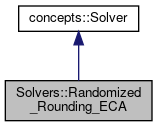
\includegraphics[width=190pt]{class_solvers_1_1_randomized___rounding___e_c_a__inherit__graph}
\end{center}
\end{figure}


Collaboration diagram for Solvers\+:\+:Randomized\+\_\+\+Rounding\+\_\+\+E\+CA\+:\nopagebreak
\begin{figure}[H]
\begin{center}
\leavevmode
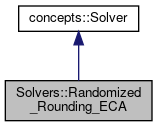
\includegraphics[width=190pt]{class_solvers_1_1_randomized___rounding___e_c_a__coll__graph}
\end{center}
\end{figure}
\subsection*{Public Member Functions}
\begin{DoxyCompactItemize}
\item 
\hyperlink{class_solvers_1_1_randomized___rounding___e_c_a_a81b6832c2158a779130e23d9949aa3f8}{Randomized\+\_\+\+Rounding\+\_\+\+E\+CA} ()
\item 
\hyperlink{class_solvers_1_1_randomized___rounding___e_c_a}{Randomized\+\_\+\+Rounding\+\_\+\+E\+CA} \& \hyperlink{class_solvers_1_1_randomized___rounding___e_c_a_a45af530a702b2f933a3723531eb0e571}{set\+Log\+Level} (int log\+\_\+level)
\item 
\hyperlink{class_solvers_1_1_randomized___rounding___e_c_a}{Randomized\+\_\+\+Rounding\+\_\+\+E\+CA} \& \hyperlink{class_solvers_1_1_randomized___rounding___e_c_a_aba0b81a8be1a129086420decd51df069}{set\+Nb\+Draws} (int log\+\_\+level)
\item 
\hyperlink{class_solvers_1_1_randomized___rounding___e_c_a}{Randomized\+\_\+\+Rounding\+\_\+\+E\+CA} \& \hyperlink{class_solvers_1_1_randomized___rounding___e_c_a_a66ac903b915fcc755c1dd4b0f54ed6ec}{set\+Parallel} (int parallel)
\item 
\hyperlink{class_solution}{Solution} $\ast$ \hyperlink{class_solvers_1_1_randomized___rounding___e_c_a_a2b2c1f0da1e047a5add3fd1bb5e6f0e8}{solve} (const \hyperlink{class_landscape}{Landscape} \&landscape, const \hyperlink{class_restoration_plan}{Restoration\+Plan} \&plans, const double B) const
\item 
const std\+::string \hyperlink{class_solvers_1_1_randomized___rounding___e_c_a_aa9ae623007f23dbd73d367649021c8a9}{name} () const
\end{DoxyCompactItemize}
\subsection*{Additional Inherited Members}


\subsection{Constructor \& Destructor Documentation}
\mbox{\Hypertarget{class_solvers_1_1_randomized___rounding___e_c_a_a81b6832c2158a779130e23d9949aa3f8}\label{class_solvers_1_1_randomized___rounding___e_c_a_a81b6832c2158a779130e23d9949aa3f8}} 
\index{Solvers\+::\+Randomized\+\_\+\+Rounding\+\_\+\+E\+CA@{Solvers\+::\+Randomized\+\_\+\+Rounding\+\_\+\+E\+CA}!Randomized\+\_\+\+Rounding\+\_\+\+E\+CA@{Randomized\+\_\+\+Rounding\+\_\+\+E\+CA}}
\index{Randomized\+\_\+\+Rounding\+\_\+\+E\+CA@{Randomized\+\_\+\+Rounding\+\_\+\+E\+CA}!Solvers\+::\+Randomized\+\_\+\+Rounding\+\_\+\+E\+CA@{Solvers\+::\+Randomized\+\_\+\+Rounding\+\_\+\+E\+CA}}
\subsubsection{\texorpdfstring{Randomized\+\_\+\+Rounding\+\_\+\+E\+C\+A()}{Randomized\_Rounding\_ECA()}}
{\footnotesize\ttfamily Solvers\+::\+Randomized\+\_\+\+Rounding\+\_\+\+E\+C\+A\+::\+Randomized\+\_\+\+Rounding\+\_\+\+E\+CA (\begin{DoxyParamCaption}{ }\end{DoxyParamCaption})\hspace{0.3cm}{\ttfamily [inline]}}



\subsection{Member Function Documentation}
\mbox{\Hypertarget{class_solvers_1_1_randomized___rounding___e_c_a_aa9ae623007f23dbd73d367649021c8a9}\label{class_solvers_1_1_randomized___rounding___e_c_a_aa9ae623007f23dbd73d367649021c8a9}} 
\index{Solvers\+::\+Randomized\+\_\+\+Rounding\+\_\+\+E\+CA@{Solvers\+::\+Randomized\+\_\+\+Rounding\+\_\+\+E\+CA}!name@{name}}
\index{name@{name}!Solvers\+::\+Randomized\+\_\+\+Rounding\+\_\+\+E\+CA@{Solvers\+::\+Randomized\+\_\+\+Rounding\+\_\+\+E\+CA}}
\subsubsection{\texorpdfstring{name()}{name()}}
{\footnotesize\ttfamily const std\+::string Solvers\+::\+Randomized\+\_\+\+Rounding\+\_\+\+E\+C\+A\+::name (\begin{DoxyParamCaption}{ }\end{DoxyParamCaption}) const\hspace{0.3cm}{\ttfamily [inline]}, {\ttfamily [virtual]}}



Implements \hyperlink{classconcepts_1_1_solver_ab995568318a506446228f45cab2fcce7}{concepts\+::\+Solver}.

\mbox{\Hypertarget{class_solvers_1_1_randomized___rounding___e_c_a_a45af530a702b2f933a3723531eb0e571}\label{class_solvers_1_1_randomized___rounding___e_c_a_a45af530a702b2f933a3723531eb0e571}} 
\index{Solvers\+::\+Randomized\+\_\+\+Rounding\+\_\+\+E\+CA@{Solvers\+::\+Randomized\+\_\+\+Rounding\+\_\+\+E\+CA}!set\+Log\+Level@{set\+Log\+Level}}
\index{set\+Log\+Level@{set\+Log\+Level}!Solvers\+::\+Randomized\+\_\+\+Rounding\+\_\+\+E\+CA@{Solvers\+::\+Randomized\+\_\+\+Rounding\+\_\+\+E\+CA}}
\subsubsection{\texorpdfstring{set\+Log\+Level()}{setLogLevel()}}
{\footnotesize\ttfamily \hyperlink{class_solvers_1_1_randomized___rounding___e_c_a}{Randomized\+\_\+\+Rounding\+\_\+\+E\+CA}\& Solvers\+::\+Randomized\+\_\+\+Rounding\+\_\+\+E\+C\+A\+::set\+Log\+Level (\begin{DoxyParamCaption}\item[{int}]{log\+\_\+level }\end{DoxyParamCaption})\hspace{0.3cm}{\ttfamily [inline]}}

\mbox{\Hypertarget{class_solvers_1_1_randomized___rounding___e_c_a_aba0b81a8be1a129086420decd51df069}\label{class_solvers_1_1_randomized___rounding___e_c_a_aba0b81a8be1a129086420decd51df069}} 
\index{Solvers\+::\+Randomized\+\_\+\+Rounding\+\_\+\+E\+CA@{Solvers\+::\+Randomized\+\_\+\+Rounding\+\_\+\+E\+CA}!set\+Nb\+Draws@{set\+Nb\+Draws}}
\index{set\+Nb\+Draws@{set\+Nb\+Draws}!Solvers\+::\+Randomized\+\_\+\+Rounding\+\_\+\+E\+CA@{Solvers\+::\+Randomized\+\_\+\+Rounding\+\_\+\+E\+CA}}
\subsubsection{\texorpdfstring{set\+Nb\+Draws()}{setNbDraws()}}
{\footnotesize\ttfamily \hyperlink{class_solvers_1_1_randomized___rounding___e_c_a}{Randomized\+\_\+\+Rounding\+\_\+\+E\+CA}\& Solvers\+::\+Randomized\+\_\+\+Rounding\+\_\+\+E\+C\+A\+::set\+Nb\+Draws (\begin{DoxyParamCaption}\item[{int}]{log\+\_\+level }\end{DoxyParamCaption})\hspace{0.3cm}{\ttfamily [inline]}}

\mbox{\Hypertarget{class_solvers_1_1_randomized___rounding___e_c_a_a66ac903b915fcc755c1dd4b0f54ed6ec}\label{class_solvers_1_1_randomized___rounding___e_c_a_a66ac903b915fcc755c1dd4b0f54ed6ec}} 
\index{Solvers\+::\+Randomized\+\_\+\+Rounding\+\_\+\+E\+CA@{Solvers\+::\+Randomized\+\_\+\+Rounding\+\_\+\+E\+CA}!set\+Parallel@{set\+Parallel}}
\index{set\+Parallel@{set\+Parallel}!Solvers\+::\+Randomized\+\_\+\+Rounding\+\_\+\+E\+CA@{Solvers\+::\+Randomized\+\_\+\+Rounding\+\_\+\+E\+CA}}
\subsubsection{\texorpdfstring{set\+Parallel()}{setParallel()}}
{\footnotesize\ttfamily \hyperlink{class_solvers_1_1_randomized___rounding___e_c_a}{Randomized\+\_\+\+Rounding\+\_\+\+E\+CA}\& Solvers\+::\+Randomized\+\_\+\+Rounding\+\_\+\+E\+C\+A\+::set\+Parallel (\begin{DoxyParamCaption}\item[{int}]{parallel }\end{DoxyParamCaption})\hspace{0.3cm}{\ttfamily [inline]}}

\mbox{\Hypertarget{class_solvers_1_1_randomized___rounding___e_c_a_a2b2c1f0da1e047a5add3fd1bb5e6f0e8}\label{class_solvers_1_1_randomized___rounding___e_c_a_a2b2c1f0da1e047a5add3fd1bb5e6f0e8}} 
\index{Solvers\+::\+Randomized\+\_\+\+Rounding\+\_\+\+E\+CA@{Solvers\+::\+Randomized\+\_\+\+Rounding\+\_\+\+E\+CA}!solve@{solve}}
\index{solve@{solve}!Solvers\+::\+Randomized\+\_\+\+Rounding\+\_\+\+E\+CA@{Solvers\+::\+Randomized\+\_\+\+Rounding\+\_\+\+E\+CA}}
\subsubsection{\texorpdfstring{solve()}{solve()}}
{\footnotesize\ttfamily \hyperlink{class_solution}{Solution} $\ast$ Solvers\+::\+Randomized\+\_\+\+Rounding\+\_\+\+E\+C\+A\+::solve (\begin{DoxyParamCaption}\item[{const \hyperlink{class_landscape}{Landscape} \&}]{landscape,  }\item[{const \hyperlink{class_restoration_plan}{Restoration\+Plan} \&}]{plans,  }\item[{const double}]{B }\end{DoxyParamCaption}) const\hspace{0.3cm}{\ttfamily [virtual]}}



Implements \hyperlink{classconcepts_1_1_solver_af323ad29df1e7b87facd7dc007568c80}{concepts\+::\+Solver}.



The documentation for this class was generated from the following files\+:\begin{DoxyCompactItemize}
\item 
/home/plaiseek/\+Projects/landscape\+\_\+opt\+\_\+cpp/include/solvers/\hyperlink{randomized__rounding_8hpp}{randomized\+\_\+rounding.\+hpp}\item 
/home/plaiseek/\+Projects/landscape\+\_\+opt\+\_\+cpp/src/solvers/\hyperlink{randomized__rounding_8cpp}{randomized\+\_\+rounding.\+cpp}\end{DoxyCompactItemize}

\hypertarget{class_restoration_plan}{}\section{Restoration\+Plan Class Reference}
\label{class_restoration_plan}\index{Restoration\+Plan@{Restoration\+Plan}}


{\ttfamily \#include $<$restoration\+\_\+plan.\+hpp$>$}

\subsection*{Classes}
\begin{DoxyCompactItemize}
\item 
class \hyperlink{class_restoration_plan_1_1_option}{Option}
\end{DoxyCompactItemize}
\subsection*{Public Member Functions}
\begin{DoxyCompactItemize}
\item 
\hyperlink{class_restoration_plan_aef8ef06f5f745bbdd598c1df66c42ca8}{Restoration\+Plan} (const \hyperlink{class_landscape}{Landscape} \&l)
\item 
\hyperlink{class_restoration_plan_ac34ea5df284566db818bebf4de22c5e7}{$\sim$\+Restoration\+Plan} ()
\item 
const \hyperlink{class_landscape}{Landscape} \& \hyperlink{class_restoration_plan_a4bbbe2c593bd9d3de466cf3ea78bf310}{get\+Landscape} () const
\item 
\hyperlink{class_restoration_plan_1_1_option}{Option} $\ast$ \hyperlink{class_restoration_plan_a4f3ae1b64679d1b191077043c5cdedb7}{add\+Option} ()
\item 
int \hyperlink{class_restoration_plan_a7c8b52ba6e6a18b25cad055a6cd3086b}{index\+Of\+Option} (\hyperlink{class_restoration_plan_1_1_option}{Option} $\ast$option)
\item 
bool \hyperlink{class_restoration_plan_a9f076ad104176e469a5e1e8aecf72614}{contains\+Option} (\hyperlink{class_restoration_plan_1_1_option}{Option} $\ast$option) const
\item 
void \hyperlink{class_restoration_plan_a69958ecdd37533b64b601f6c2f190875}{remove\+Option} (int index)
\item 
void \hyperlink{class_restoration_plan_a7ea1f7c7dcee6357b0bd3a2d868a13b9}{remove\+Option} (\hyperlink{class_restoration_plan_1_1_option}{Option} $\ast$option)
\item 
void \hyperlink{class_restoration_plan_a8be9afd54fef1a4bcd2746c8d8dca3d9}{remove\+Empty\+Options} ()
\item 
const std\+::vector$<$ \hyperlink{class_restoration_plan_1_1_option}{Option} $\ast$ $>$ \& \hyperlink{class_restoration_plan_aeeca484cdb23f784a0a40256db6327a5}{options} () const
\item 
int \hyperlink{class_restoration_plan_a7c4e4b567a22267fb6a1c7eb8617c0fa}{get\+Nb\+Options} () const
\item 
void \hyperlink{class_restoration_plan_a59da0a26384e50e4615bcffa926b2d69}{remove} (Graph\+\_\+t\+::\+Node v)
\item 
void \hyperlink{class_restoration_plan_ae75f389f03e4fcb76b691ab383452142}{remove} (Graph\+\_\+t\+::\+Arc a)
\item 
const std\+::list$<$ \hyperlink{class_restoration_plan_1_1_option}{Option} $\ast$ $>$ \& \hyperlink{class_restoration_plan_a0c27b60675feb66f08f142d2d090ea7a}{get\+Options} (Graph\+\_\+t\+::\+Node v) const
\item 
const std\+::list$<$ \hyperlink{class_restoration_plan_1_1_option}{Option} $\ast$ $>$ \& \hyperlink{class_restoration_plan_afd0c1f1d3c4a8d951a72500bfe9fa31a}{get\+Options} (Graph\+\_\+t\+::\+Arc a) const
\item 
bool \hyperlink{class_restoration_plan_a719e93c4b00658a3932dd0abf2bdacf1}{contains} (Graph\+\_\+t\+::\+Node v) const
\item 
bool \hyperlink{class_restoration_plan_a6ec10a970b2f6cac43a4dbb66232e457}{contains} (Graph\+\_\+t\+::\+Arc a) const
\item 
void \hyperlink{class_restoration_plan_ab5733bd94e4808886168fe1688636499}{clean\+Invalid\+Elements} ()
\item 
void \hyperlink{class_restoration_plan_ad00a959043a8eb29204700762ce7ae41}{print} () const
\end{DoxyCompactItemize}


\subsection{Constructor \& Destructor Documentation}
\mbox{\Hypertarget{class_restoration_plan_aef8ef06f5f745bbdd598c1df66c42ca8}\label{class_restoration_plan_aef8ef06f5f745bbdd598c1df66c42ca8}} 
\index{Restoration\+Plan@{Restoration\+Plan}!Restoration\+Plan@{Restoration\+Plan}}
\index{Restoration\+Plan@{Restoration\+Plan}!Restoration\+Plan@{Restoration\+Plan}}
\subsubsection{\texorpdfstring{Restoration\+Plan()}{RestorationPlan()}}
{\footnotesize\ttfamily Restoration\+Plan\+::\+Restoration\+Plan (\begin{DoxyParamCaption}\item[{const \hyperlink{class_landscape}{Landscape} \&}]{l }\end{DoxyParamCaption})}

\mbox{\Hypertarget{class_restoration_plan_ac34ea5df284566db818bebf4de22c5e7}\label{class_restoration_plan_ac34ea5df284566db818bebf4de22c5e7}} 
\index{Restoration\+Plan@{Restoration\+Plan}!````~Restoration\+Plan@{$\sim$\+Restoration\+Plan}}
\index{````~Restoration\+Plan@{$\sim$\+Restoration\+Plan}!Restoration\+Plan@{Restoration\+Plan}}
\subsubsection{\texorpdfstring{$\sim$\+Restoration\+Plan()}{~RestorationPlan()}}
{\footnotesize\ttfamily Restoration\+Plan\+::$\sim$\+Restoration\+Plan (\begin{DoxyParamCaption}{ }\end{DoxyParamCaption})}



\subsection{Member Function Documentation}
\mbox{\Hypertarget{class_restoration_plan_a4f3ae1b64679d1b191077043c5cdedb7}\label{class_restoration_plan_a4f3ae1b64679d1b191077043c5cdedb7}} 
\index{Restoration\+Plan@{Restoration\+Plan}!add\+Option@{add\+Option}}
\index{add\+Option@{add\+Option}!Restoration\+Plan@{Restoration\+Plan}}
\subsubsection{\texorpdfstring{add\+Option()}{addOption()}}
{\footnotesize\ttfamily \hyperlink{class_restoration_plan_1_1_option}{Restoration\+Plan\+::\+Option} $\ast$ Restoration\+Plan\+::add\+Option (\begin{DoxyParamCaption}{ }\end{DoxyParamCaption})}

\mbox{\Hypertarget{class_restoration_plan_ab5733bd94e4808886168fe1688636499}\label{class_restoration_plan_ab5733bd94e4808886168fe1688636499}} 
\index{Restoration\+Plan@{Restoration\+Plan}!clean\+Invalid\+Elements@{clean\+Invalid\+Elements}}
\index{clean\+Invalid\+Elements@{clean\+Invalid\+Elements}!Restoration\+Plan@{Restoration\+Plan}}
\subsubsection{\texorpdfstring{clean\+Invalid\+Elements()}{cleanInvalidElements()}}
{\footnotesize\ttfamily void Restoration\+Plan\+::clean\+Invalid\+Elements (\begin{DoxyParamCaption}{ }\end{DoxyParamCaption})}

\mbox{\Hypertarget{class_restoration_plan_a719e93c4b00658a3932dd0abf2bdacf1}\label{class_restoration_plan_a719e93c4b00658a3932dd0abf2bdacf1}} 
\index{Restoration\+Plan@{Restoration\+Plan}!contains@{contains}}
\index{contains@{contains}!Restoration\+Plan@{Restoration\+Plan}}
\subsubsection{\texorpdfstring{contains()}{contains()}\hspace{0.1cm}{\footnotesize\ttfamily [1/2]}}
{\footnotesize\ttfamily bool Restoration\+Plan\+::contains (\begin{DoxyParamCaption}\item[{Graph\+\_\+t\+::\+Node}]{v }\end{DoxyParamCaption}) const}

\mbox{\Hypertarget{class_restoration_plan_a6ec10a970b2f6cac43a4dbb66232e457}\label{class_restoration_plan_a6ec10a970b2f6cac43a4dbb66232e457}} 
\index{Restoration\+Plan@{Restoration\+Plan}!contains@{contains}}
\index{contains@{contains}!Restoration\+Plan@{Restoration\+Plan}}
\subsubsection{\texorpdfstring{contains()}{contains()}\hspace{0.1cm}{\footnotesize\ttfamily [2/2]}}
{\footnotesize\ttfamily bool Restoration\+Plan\+::contains (\begin{DoxyParamCaption}\item[{Graph\+\_\+t\+::\+Arc}]{a }\end{DoxyParamCaption}) const}

\mbox{\Hypertarget{class_restoration_plan_a9f076ad104176e469a5e1e8aecf72614}\label{class_restoration_plan_a9f076ad104176e469a5e1e8aecf72614}} 
\index{Restoration\+Plan@{Restoration\+Plan}!contains\+Option@{contains\+Option}}
\index{contains\+Option@{contains\+Option}!Restoration\+Plan@{Restoration\+Plan}}
\subsubsection{\texorpdfstring{contains\+Option()}{containsOption()}}
{\footnotesize\ttfamily bool Restoration\+Plan\+::contains\+Option (\begin{DoxyParamCaption}\item[{\hyperlink{class_restoration_plan_1_1_option}{Option} $\ast$}]{option }\end{DoxyParamCaption}) const}

\mbox{\Hypertarget{class_restoration_plan_a4bbbe2c593bd9d3de466cf3ea78bf310}\label{class_restoration_plan_a4bbbe2c593bd9d3de466cf3ea78bf310}} 
\index{Restoration\+Plan@{Restoration\+Plan}!get\+Landscape@{get\+Landscape}}
\index{get\+Landscape@{get\+Landscape}!Restoration\+Plan@{Restoration\+Plan}}
\subsubsection{\texorpdfstring{get\+Landscape()}{getLandscape()}}
{\footnotesize\ttfamily const \hyperlink{class_landscape}{Landscape} \& Restoration\+Plan\+::get\+Landscape (\begin{DoxyParamCaption}{ }\end{DoxyParamCaption}) const}

\mbox{\Hypertarget{class_restoration_plan_a7c4e4b567a22267fb6a1c7eb8617c0fa}\label{class_restoration_plan_a7c4e4b567a22267fb6a1c7eb8617c0fa}} 
\index{Restoration\+Plan@{Restoration\+Plan}!get\+Nb\+Options@{get\+Nb\+Options}}
\index{get\+Nb\+Options@{get\+Nb\+Options}!Restoration\+Plan@{Restoration\+Plan}}
\subsubsection{\texorpdfstring{get\+Nb\+Options()}{getNbOptions()}}
{\footnotesize\ttfamily int Restoration\+Plan\+::get\+Nb\+Options (\begin{DoxyParamCaption}{ }\end{DoxyParamCaption}) const}

\mbox{\Hypertarget{class_restoration_plan_a0c27b60675feb66f08f142d2d090ea7a}\label{class_restoration_plan_a0c27b60675feb66f08f142d2d090ea7a}} 
\index{Restoration\+Plan@{Restoration\+Plan}!get\+Options@{get\+Options}}
\index{get\+Options@{get\+Options}!Restoration\+Plan@{Restoration\+Plan}}
\subsubsection{\texorpdfstring{get\+Options()}{getOptions()}\hspace{0.1cm}{\footnotesize\ttfamily [1/2]}}
{\footnotesize\ttfamily const std\+::list$<$ \hyperlink{class_restoration_plan_1_1_option}{Restoration\+Plan\+::\+Option} $\ast$ $>$ \& Restoration\+Plan\+::get\+Options (\begin{DoxyParamCaption}\item[{Graph\+\_\+t\+::\+Node}]{v }\end{DoxyParamCaption}) const}

\mbox{\Hypertarget{class_restoration_plan_afd0c1f1d3c4a8d951a72500bfe9fa31a}\label{class_restoration_plan_afd0c1f1d3c4a8d951a72500bfe9fa31a}} 
\index{Restoration\+Plan@{Restoration\+Plan}!get\+Options@{get\+Options}}
\index{get\+Options@{get\+Options}!Restoration\+Plan@{Restoration\+Plan}}
\subsubsection{\texorpdfstring{get\+Options()}{getOptions()}\hspace{0.1cm}{\footnotesize\ttfamily [2/2]}}
{\footnotesize\ttfamily const std\+::list$<$ \hyperlink{class_restoration_plan_1_1_option}{Restoration\+Plan\+::\+Option} $\ast$ $>$ \& Restoration\+Plan\+::get\+Options (\begin{DoxyParamCaption}\item[{Graph\+\_\+t\+::\+Arc}]{a }\end{DoxyParamCaption}) const}

\mbox{\Hypertarget{class_restoration_plan_a7c8b52ba6e6a18b25cad055a6cd3086b}\label{class_restoration_plan_a7c8b52ba6e6a18b25cad055a6cd3086b}} 
\index{Restoration\+Plan@{Restoration\+Plan}!index\+Of\+Option@{index\+Of\+Option}}
\index{index\+Of\+Option@{index\+Of\+Option}!Restoration\+Plan@{Restoration\+Plan}}
\subsubsection{\texorpdfstring{index\+Of\+Option()}{indexOfOption()}}
{\footnotesize\ttfamily int Restoration\+Plan\+::index\+Of\+Option (\begin{DoxyParamCaption}\item[{\hyperlink{class_restoration_plan_1_1_option}{Restoration\+Plan\+::\+Option} $\ast$}]{option }\end{DoxyParamCaption})}

\mbox{\Hypertarget{class_restoration_plan_aeeca484cdb23f784a0a40256db6327a5}\label{class_restoration_plan_aeeca484cdb23f784a0a40256db6327a5}} 
\index{Restoration\+Plan@{Restoration\+Plan}!options@{options}}
\index{options@{options}!Restoration\+Plan@{Restoration\+Plan}}
\subsubsection{\texorpdfstring{options()}{options()}}
{\footnotesize\ttfamily const std\+::vector$<$ \hyperlink{class_restoration_plan_1_1_option}{Restoration\+Plan\+::\+Option} $\ast$ $>$ \& Restoration\+Plan\+::options (\begin{DoxyParamCaption}{ }\end{DoxyParamCaption}) const}

\mbox{\Hypertarget{class_restoration_plan_ad00a959043a8eb29204700762ce7ae41}\label{class_restoration_plan_ad00a959043a8eb29204700762ce7ae41}} 
\index{Restoration\+Plan@{Restoration\+Plan}!print@{print}}
\index{print@{print}!Restoration\+Plan@{Restoration\+Plan}}
\subsubsection{\texorpdfstring{print()}{print()}}
{\footnotesize\ttfamily void Restoration\+Plan\+::print (\begin{DoxyParamCaption}{ }\end{DoxyParamCaption}) const}

\mbox{\Hypertarget{class_restoration_plan_a59da0a26384e50e4615bcffa926b2d69}\label{class_restoration_plan_a59da0a26384e50e4615bcffa926b2d69}} 
\index{Restoration\+Plan@{Restoration\+Plan}!remove@{remove}}
\index{remove@{remove}!Restoration\+Plan@{Restoration\+Plan}}
\subsubsection{\texorpdfstring{remove()}{remove()}\hspace{0.1cm}{\footnotesize\ttfamily [1/2]}}
{\footnotesize\ttfamily void Restoration\+Plan\+::remove (\begin{DoxyParamCaption}\item[{Graph\+\_\+t\+::\+Node}]{v }\end{DoxyParamCaption})}

\mbox{\Hypertarget{class_restoration_plan_ae75f389f03e4fcb76b691ab383452142}\label{class_restoration_plan_ae75f389f03e4fcb76b691ab383452142}} 
\index{Restoration\+Plan@{Restoration\+Plan}!remove@{remove}}
\index{remove@{remove}!Restoration\+Plan@{Restoration\+Plan}}
\subsubsection{\texorpdfstring{remove()}{remove()}\hspace{0.1cm}{\footnotesize\ttfamily [2/2]}}
{\footnotesize\ttfamily void Restoration\+Plan\+::remove (\begin{DoxyParamCaption}\item[{Graph\+\_\+t\+::\+Arc}]{a }\end{DoxyParamCaption})}

\mbox{\Hypertarget{class_restoration_plan_a8be9afd54fef1a4bcd2746c8d8dca3d9}\label{class_restoration_plan_a8be9afd54fef1a4bcd2746c8d8dca3d9}} 
\index{Restoration\+Plan@{Restoration\+Plan}!remove\+Empty\+Options@{remove\+Empty\+Options}}
\index{remove\+Empty\+Options@{remove\+Empty\+Options}!Restoration\+Plan@{Restoration\+Plan}}
\subsubsection{\texorpdfstring{remove\+Empty\+Options()}{removeEmptyOptions()}}
{\footnotesize\ttfamily void Restoration\+Plan\+::remove\+Empty\+Options (\begin{DoxyParamCaption}{ }\end{DoxyParamCaption})}

\mbox{\Hypertarget{class_restoration_plan_a69958ecdd37533b64b601f6c2f190875}\label{class_restoration_plan_a69958ecdd37533b64b601f6c2f190875}} 
\index{Restoration\+Plan@{Restoration\+Plan}!remove\+Option@{remove\+Option}}
\index{remove\+Option@{remove\+Option}!Restoration\+Plan@{Restoration\+Plan}}
\subsubsection{\texorpdfstring{remove\+Option()}{removeOption()}\hspace{0.1cm}{\footnotesize\ttfamily [1/2]}}
{\footnotesize\ttfamily void Restoration\+Plan\+::remove\+Option (\begin{DoxyParamCaption}\item[{int}]{index }\end{DoxyParamCaption})}

\mbox{\Hypertarget{class_restoration_plan_a7ea1f7c7dcee6357b0bd3a2d868a13b9}\label{class_restoration_plan_a7ea1f7c7dcee6357b0bd3a2d868a13b9}} 
\index{Restoration\+Plan@{Restoration\+Plan}!remove\+Option@{remove\+Option}}
\index{remove\+Option@{remove\+Option}!Restoration\+Plan@{Restoration\+Plan}}
\subsubsection{\texorpdfstring{remove\+Option()}{removeOption()}\hspace{0.1cm}{\footnotesize\ttfamily [2/2]}}
{\footnotesize\ttfamily void Restoration\+Plan\+::remove\+Option (\begin{DoxyParamCaption}\item[{\hyperlink{class_restoration_plan_1_1_option}{Restoration\+Plan\+::\+Option} $\ast$}]{option }\end{DoxyParamCaption})}



The documentation for this class was generated from the following files\+:\begin{DoxyCompactItemize}
\item 
/home/plaiseek/\+Projects/landscape\+\_\+opt\+\_\+cpp/include/solvers/concept/\hyperlink{restoration__plan_8hpp}{restoration\+\_\+plan.\+hpp}\item 
/home/plaiseek/\+Projects/landscape\+\_\+opt\+\_\+cpp/src/solvers/concept/\hyperlink{restoration__plan_8cpp}{restoration\+\_\+plan.\+cpp}\end{DoxyCompactItemize}

\hypertarget{class_restoration_plan2}{}\section{Restoration\+Plan2 Class Reference}
\label{class_restoration_plan2}\index{Restoration\+Plan2@{Restoration\+Plan2}}


A class for respresenting a restoration plan.  




{\ttfamily \#include $<$restoration\+\_\+plan\+\_\+2.\+hpp$>$}

\subsection*{Public Types}
\begin{DoxyCompactItemize}
\item 
typedef int \hyperlink{class_restoration_plan2_aff164a2726831342bf87af5e11df1064}{Option}
\end{DoxyCompactItemize}
\subsection*{Public Member Functions}
\begin{DoxyCompactItemize}
\item 
\hyperlink{class_restoration_plan2_a9f7a6a7f8421ba8f94601cb00c8effc4}{Restoration\+Plan2} (const \hyperlink{class_landscape}{Landscape} \&l)
\item 
\hyperlink{class_restoration_plan2_ae0f4cdb50c5e051f054a7662b1de91d3}{$\sim$\+Restoration\+Plan2} ()
\item 
const \hyperlink{class_landscape}{Landscape} \& \hyperlink{class_restoration_plan2_a15d5303518cb31378111c8da175dc659}{get\+Landscape} () const
\item 
int \hyperlink{class_restoration_plan2_a300dbff4b8071a136682b5350bb916a2}{get\+Nb\+Nodes} (\hyperlink{class_restoration_plan2_aff164a2726831342bf87af5e11df1064}{Option} i) const
\begin{DoxyCompactList}\small\item\em Get the number of nodes concerned by option {\bfseries i} \end{DoxyCompactList}\item 
int \hyperlink{class_restoration_plan2_a91230a516340063f605ab295ae7f31d3}{get\+Nb\+Arcs} (\hyperlink{class_restoration_plan2_aff164a2726831342bf87af5e11df1064}{Option} i) const
\begin{DoxyCompactList}\small\item\em Get the number of arcs concerned by option {\bfseries i} \end{DoxyCompactList}\item 
bool \hyperlink{class_restoration_plan2_acf5e11d698c3306efeafaa5ca5d6f3ed}{contains} (\hyperlink{class_restoration_plan2_aff164a2726831342bf87af5e11df1064}{Option} i, Graph\+\_\+t\+::\+Node v) const
\begin{DoxyCompactList}\small\item\em Return true if the option {\bfseries i} concerns node {\bfseries v} \end{DoxyCompactList}\item 
bool \hyperlink{class_restoration_plan2_a1884daec27de69af8302b961aee1b232}{contains} (\hyperlink{class_restoration_plan2_aff164a2726831342bf87af5e11df1064}{Option} i, Graph\+\_\+t\+::\+Arc a) const
\begin{DoxyCompactList}\small\item\em Return true if the option {\bfseries i} concerns arc {\bfseries a} \end{DoxyCompactList}\item 
bool \hyperlink{class_restoration_plan2_a753668d5ba34ea1e088aee85218543b7}{contains} (Graph\+\_\+t\+::\+Node v) const
\begin{DoxyCompactList}\small\item\em Test if there is an option concerning the node {\bfseries v} \end{DoxyCompactList}\item 
bool \hyperlink{class_restoration_plan2_acac88b4dcb361cf6ca3061457ff05bfa}{contains} (Graph\+\_\+t\+::\+Arc a) const
\begin{DoxyCompactList}\small\item\em Test if there is an option concerning the arc {\bfseries a} \end{DoxyCompactList}\item 
void \hyperlink{class_restoration_plan2_a0a5a2740cdea0ec03ffa9c5d1d94a202}{add\+Node} (\hyperlink{class_restoration_plan2_aff164a2726831342bf87af5e11df1064}{Option} i, Graph\+\_\+t\+::\+Node v, double quality\+\_\+gain)
\begin{DoxyCompactList}\small\item\em Add the node {\bfseries v} to the option {\bfseries i} \end{DoxyCompactList}\item 
void \hyperlink{class_restoration_plan2_a37dd2e978ecb5e36fa2c35e5025cf729}{add\+Arc} (\hyperlink{class_restoration_plan2_aff164a2726831342bf87af5e11df1064}{Option} i, Graph\+\_\+t\+::\+Arc a, double restored\+\_\+probability)
\begin{DoxyCompactList}\small\item\em Add the arc {\bfseries a} to the option {\bfseries i} \end{DoxyCompactList}\item 
void \hyperlink{class_restoration_plan2_a845fbee26cdfc01d689c7c24f55f0c31}{remove\+Node} (\hyperlink{class_restoration_plan2_aff164a2726831342bf87af5e11df1064}{Option} i, Graph\+\_\+t\+::\+Node v)
\begin{DoxyCompactList}\small\item\em Remove the node {\bfseries v} from the option {\bfseries i} \end{DoxyCompactList}\item 
void \hyperlink{class_restoration_plan2_a20f26b0167d527be6d60614b4cba4dbf}{remove\+Arc} (\hyperlink{class_restoration_plan2_aff164a2726831342bf87af5e11df1064}{Option} i, Graph\+\_\+t\+::\+Arc a)
\begin{DoxyCompactList}\small\item\em Remove the arc {\bfseries a} from the option {\bfseries i} \end{DoxyCompactList}\item 
void \hyperlink{class_restoration_plan2_acd618be603d5562d48c0ece65210750f}{remove\+Node} (Graph\+\_\+t\+::\+Node v)
\begin{DoxyCompactList}\small\item\em Remove the node {\bfseries v} from every option. \end{DoxyCompactList}\item 
void \hyperlink{class_restoration_plan2_aacd1be30356c999259bb98c2869bbb95}{remove\+Arc} (Graph\+\_\+t\+::\+Arc a)
\begin{DoxyCompactList}\small\item\em Remove the arc {\bfseries a} from every option. \end{DoxyCompactList}\item 
double \hyperlink{class_restoration_plan2_a55e84c9117d460224ea5e30f77e13b16}{get\+Quality\+Gain} (\hyperlink{class_restoration_plan2_aff164a2726831342bf87af5e11df1064}{Option} i, Graph\+\_\+t\+::\+Node v) const
\begin{DoxyCompactList}\small\item\em Get the Quality\+Gain of node {\bfseries v} in the option {\bfseries i} \end{DoxyCompactList}\item 
double \hyperlink{class_restoration_plan2_a22980a28d0904266602a16542fa75110}{get\+Restored\+Probability} (\hyperlink{class_restoration_plan2_aff164a2726831342bf87af5e11df1064}{Option} i, Graph\+\_\+t\+::\+Arc a) const
\begin{DoxyCompactList}\small\item\em Get the Restored\+Probability of arc {\bfseries a} in the option {\bfseries i} \end{DoxyCompactList}\item 
double \hyperlink{class_restoration_plan2_ab57f10bed72f50c27438e6dc06f57ca6}{id} (\hyperlink{class_restoration_plan2_aff164a2726831342bf87af5e11df1064}{Option} i, Graph\+\_\+t\+::\+Node v) const
\begin{DoxyCompactList}\small\item\em Get the id of the node {\bfseries v} in the option {\bfseries i} \end{DoxyCompactList}\item 
double \hyperlink{class_restoration_plan2_a8967a613c2f9cbabb2418217abfe8e74}{id} (\hyperlink{class_restoration_plan2_aff164a2726831342bf87af5e11df1064}{Option} i, Graph\+\_\+t\+::\+Arc a) const
\begin{DoxyCompactList}\small\item\em Get the id of the arc {\bfseries a} in the option {\bfseries i} \end{DoxyCompactList}\item 
\hyperlink{class_restoration_plan2_aff164a2726831342bf87af5e11df1064}{Option} \hyperlink{class_restoration_plan2_a7461e5c0cd622f9e6adbf38f34753a07}{add\+Option} (double c)
\begin{DoxyCompactList}\small\item\em add an option of cost {\bfseries c} and returns its id \end{DoxyCompactList}\item 
void \hyperlink{class_restoration_plan2_aea25e41ec7132080a756a57cde477c65}{set\+Cost} (\hyperlink{class_restoration_plan2_aff164a2726831342bf87af5e11df1064}{Option} i, double cost)
\begin{DoxyCompactList}\small\item\em Set the cost of option {\bfseries i} \end{DoxyCompactList}\item 
double \hyperlink{class_restoration_plan2_abac73d19450c44e9a96ab8ef680af044}{get\+Cost} (\hyperlink{class_restoration_plan2_aff164a2726831342bf87af5e11df1064}{Option} i) const
\begin{DoxyCompactList}\small\item\em Get the cost of option {\bfseries i} \end{DoxyCompactList}\item 
bool \hyperlink{class_restoration_plan2_af4810bc9bb239488322ab53b72c30a44}{is\+Empty} (\hyperlink{class_restoration_plan2_aff164a2726831342bf87af5e11df1064}{Option} i) const
\begin{DoxyCompactList}\small\item\em Test if option {\bfseries i} is empty. \end{DoxyCompactList}\item 
int \hyperlink{class_restoration_plan2_a0c69c9a149143042a88408abefe8f005}{get\+Nb\+Options} () const
\begin{DoxyCompactList}\small\item\em Get the number of options. \end{DoxyCompactList}\item 
const std\+::map$<$ \hyperlink{class_restoration_plan2_aff164a2726831342bf87af5e11df1064}{Option}, double $>$ \& \hyperlink{class_restoration_plan2_ad5677cfb92c07bdfa6c3414940ae6401}{get\+Options} (Graph\+\_\+t\+::\+Node v) const
\begin{DoxyCompactList}\small\item\em Returns the map of options concerning the node {\bfseries v} \end{DoxyCompactList}\item 
const std\+::map$<$ \hyperlink{class_restoration_plan2_aff164a2726831342bf87af5e11df1064}{Option}, double $>$ \& \hyperlink{class_restoration_plan2_a04acf02934f7b06d3540c2bc68de73d0}{get\+Options} (Graph\+\_\+t\+::\+Arc a) const
\begin{DoxyCompactList}\small\item\em Returns the map of options concerning the arc {\bfseries a} \end{DoxyCompactList}\item 
void \hyperlink{class_restoration_plan2_a5258c8409176279c8bab604400722b25}{erase\+Invalid\+Nodes} ()
\begin{DoxyCompactList}\small\item\em Erase invalid nodes from the restoration plan. \end{DoxyCompactList}\item 
void \hyperlink{class_restoration_plan2_a51e5a2f223e0cbd8763f0ff60c8a4599}{erase\+Invalid\+Arcs} ()
\begin{DoxyCompactList}\small\item\em Erase invalid nodes from the restoration plan. \end{DoxyCompactList}\item 
void \hyperlink{class_restoration_plan2_aeb925e92d2141fe96979538f087c277a}{erase\+Invalid\+Elements} ()
\begin{DoxyCompactList}\small\item\em Erase invalid nodes and arcs from the restoration plan. \end{DoxyCompactList}\end{DoxyCompactItemize}


\subsection{Detailed Description}
A class for respresenting a restoration plan. 

This class is essentially a sparse matrix implementation with both row major and column major structures to ensure linear time iteration. 

\subsection{Member Typedef Documentation}
\mbox{\Hypertarget{class_restoration_plan2_aff164a2726831342bf87af5e11df1064}\label{class_restoration_plan2_aff164a2726831342bf87af5e11df1064}} 
\index{Restoration\+Plan2@{Restoration\+Plan2}!Option@{Option}}
\index{Option@{Option}!Restoration\+Plan2@{Restoration\+Plan2}}
\subsubsection{\texorpdfstring{Option}{Option}}
{\footnotesize\ttfamily typedef int \hyperlink{class_restoration_plan2_aff164a2726831342bf87af5e11df1064}{Restoration\+Plan2\+::\+Option}}



\subsection{Constructor \& Destructor Documentation}
\mbox{\Hypertarget{class_restoration_plan2_a9f7a6a7f8421ba8f94601cb00c8effc4}\label{class_restoration_plan2_a9f7a6a7f8421ba8f94601cb00c8effc4}} 
\index{Restoration\+Plan2@{Restoration\+Plan2}!Restoration\+Plan2@{Restoration\+Plan2}}
\index{Restoration\+Plan2@{Restoration\+Plan2}!Restoration\+Plan2@{Restoration\+Plan2}}
\subsubsection{\texorpdfstring{Restoration\+Plan2()}{RestorationPlan2()}}
{\footnotesize\ttfamily Restoration\+Plan2\+::\+Restoration\+Plan2 (\begin{DoxyParamCaption}\item[{const \hyperlink{class_landscape}{Landscape} \&}]{l }\end{DoxyParamCaption})\hspace{0.3cm}{\ttfamily [inline]}}

\mbox{\Hypertarget{class_restoration_plan2_ae0f4cdb50c5e051f054a7662b1de91d3}\label{class_restoration_plan2_ae0f4cdb50c5e051f054a7662b1de91d3}} 
\index{Restoration\+Plan2@{Restoration\+Plan2}!````~Restoration\+Plan2@{$\sim$\+Restoration\+Plan2}}
\index{````~Restoration\+Plan2@{$\sim$\+Restoration\+Plan2}!Restoration\+Plan2@{Restoration\+Plan2}}
\subsubsection{\texorpdfstring{$\sim$\+Restoration\+Plan2()}{~RestorationPlan2()}}
{\footnotesize\ttfamily Restoration\+Plan2\+::$\sim$\+Restoration\+Plan2 (\begin{DoxyParamCaption}{ }\end{DoxyParamCaption})\hspace{0.3cm}{\ttfamily [inline]}}



\subsection{Member Function Documentation}
\mbox{\Hypertarget{class_restoration_plan2_a37dd2e978ecb5e36fa2c35e5025cf729}\label{class_restoration_plan2_a37dd2e978ecb5e36fa2c35e5025cf729}} 
\index{Restoration\+Plan2@{Restoration\+Plan2}!add\+Arc@{add\+Arc}}
\index{add\+Arc@{add\+Arc}!Restoration\+Plan2@{Restoration\+Plan2}}
\subsubsection{\texorpdfstring{add\+Arc()}{addArc()}}
{\footnotesize\ttfamily void Restoration\+Plan2\+::add\+Arc (\begin{DoxyParamCaption}\item[{\hyperlink{class_restoration_plan2_aff164a2726831342bf87af5e11df1064}{Option}}]{i,  }\item[{Graph\+\_\+t\+::\+Arc}]{a,  }\item[{double}]{restored\+\_\+probability }\end{DoxyParamCaption})\hspace{0.3cm}{\ttfamily [inline]}}



Add the arc {\bfseries a} to the option {\bfseries i} 


\begin{DoxyParams}{Parameters}
{\em i} & -\/ Option \\
\hline
{\em a} & -\/ Arc \\
\hline
{\em restored\+\_\+probability} & -\/ restored probability of {\bfseries a} \\
\hline
\end{DoxyParams}
\begin{DoxyRefDesc}{Time Complexity}
\item[\hyperlink{time__time000014}{Time Complexity}]$O(\log \#arcs(i) + \log \#options(a))$ \end{DoxyRefDesc}
\begin{DoxyRefDesc}{Space Complexity}
\item[\hyperlink{space__space000014}{Space Complexity}]$O(1)$ \end{DoxyRefDesc}
\mbox{\Hypertarget{class_restoration_plan2_a0a5a2740cdea0ec03ffa9c5d1d94a202}\label{class_restoration_plan2_a0a5a2740cdea0ec03ffa9c5d1d94a202}} 
\index{Restoration\+Plan2@{Restoration\+Plan2}!add\+Node@{add\+Node}}
\index{add\+Node@{add\+Node}!Restoration\+Plan2@{Restoration\+Plan2}}
\subsubsection{\texorpdfstring{add\+Node()}{addNode()}}
{\footnotesize\ttfamily void Restoration\+Plan2\+::add\+Node (\begin{DoxyParamCaption}\item[{\hyperlink{class_restoration_plan2_aff164a2726831342bf87af5e11df1064}{Option}}]{i,  }\item[{Graph\+\_\+t\+::\+Node}]{v,  }\item[{double}]{quality\+\_\+gain }\end{DoxyParamCaption})\hspace{0.3cm}{\ttfamily [inline]}}



Add the node {\bfseries v} to the option {\bfseries i} 


\begin{DoxyParams}{Parameters}
{\em i} & -\/ Option \\
\hline
{\em v} & -\/ Node \\
\hline
{\em quality\+\_\+gain} & -\/ quality gain on {\bfseries v} \\
\hline
\end{DoxyParams}
\begin{DoxyRefDesc}{Time Complexity}
\item[\hyperlink{time__time000013}{Time Complexity}]$O(\log \#nodes(i) + \log \#options(v))$ \end{DoxyRefDesc}
\begin{DoxyRefDesc}{Space Complexity}
\item[\hyperlink{space__space000013}{Space Complexity}]$O(1)$ \end{DoxyRefDesc}
\mbox{\Hypertarget{class_restoration_plan2_a7461e5c0cd622f9e6adbf38f34753a07}\label{class_restoration_plan2_a7461e5c0cd622f9e6adbf38f34753a07}} 
\index{Restoration\+Plan2@{Restoration\+Plan2}!add\+Option@{add\+Option}}
\index{add\+Option@{add\+Option}!Restoration\+Plan2@{Restoration\+Plan2}}
\subsubsection{\texorpdfstring{add\+Option()}{addOption()}}
{\footnotesize\ttfamily \hyperlink{class_restoration_plan2_aff164a2726831342bf87af5e11df1064}{Option} Restoration\+Plan2\+::add\+Option (\begin{DoxyParamCaption}\item[{double}]{c }\end{DoxyParamCaption})\hspace{0.3cm}{\ttfamily [inline]}}



add an option of cost {\bfseries c} and returns its id 


\begin{DoxyParams}{Parameters}
{\em c} & -\/ cost \\
\hline
\end{DoxyParams}
\begin{DoxyReturn}{Returns}
Option 
\end{DoxyReturn}
\begin{DoxyRefDesc}{Time Complexity}
\item[\hyperlink{time__time000023}{Time Complexity}]$O(1)$ \end{DoxyRefDesc}
\begin{DoxyRefDesc}{Space Complexity}
\item[\hyperlink{space__space000023}{Space Complexity}]$O(1)$ \end{DoxyRefDesc}
\mbox{\Hypertarget{class_restoration_plan2_acf5e11d698c3306efeafaa5ca5d6f3ed}\label{class_restoration_plan2_acf5e11d698c3306efeafaa5ca5d6f3ed}} 
\index{Restoration\+Plan2@{Restoration\+Plan2}!contains@{contains}}
\index{contains@{contains}!Restoration\+Plan2@{Restoration\+Plan2}}
\subsubsection{\texorpdfstring{contains()}{contains()}\hspace{0.1cm}{\footnotesize\ttfamily [1/4]}}
{\footnotesize\ttfamily bool Restoration\+Plan2\+::contains (\begin{DoxyParamCaption}\item[{\hyperlink{class_restoration_plan2_aff164a2726831342bf87af5e11df1064}{Option}}]{i,  }\item[{Graph\+\_\+t\+::\+Node}]{v }\end{DoxyParamCaption}) const\hspace{0.3cm}{\ttfamily [inline]}}



Return true if the option {\bfseries i} concerns node {\bfseries v} 


\begin{DoxyParams}{Parameters}
{\em i} & -\/ Option \\
\hline
{\em v} & -\/ Node \\
\hline
\end{DoxyParams}
\begin{DoxyReturn}{Returns}
bool true if the option {\bfseries i} concerns node {\bfseries v} false otherwise 
\end{DoxyReturn}
\begin{DoxyRefDesc}{Time Complexity}
\item[\hyperlink{time__time000009}{Time Complexity}]$O(\log \#nodes(i))$ \end{DoxyRefDesc}
\begin{DoxyRefDesc}{Space Complexity}
\item[\hyperlink{space__space000009}{Space Complexity}]$O(1)$ \end{DoxyRefDesc}
\mbox{\Hypertarget{class_restoration_plan2_a1884daec27de69af8302b961aee1b232}\label{class_restoration_plan2_a1884daec27de69af8302b961aee1b232}} 
\index{Restoration\+Plan2@{Restoration\+Plan2}!contains@{contains}}
\index{contains@{contains}!Restoration\+Plan2@{Restoration\+Plan2}}
\subsubsection{\texorpdfstring{contains()}{contains()}\hspace{0.1cm}{\footnotesize\ttfamily [2/4]}}
{\footnotesize\ttfamily bool Restoration\+Plan2\+::contains (\begin{DoxyParamCaption}\item[{\hyperlink{class_restoration_plan2_aff164a2726831342bf87af5e11df1064}{Option}}]{i,  }\item[{Graph\+\_\+t\+::\+Arc}]{a }\end{DoxyParamCaption}) const\hspace{0.3cm}{\ttfamily [inline]}}



Return true if the option {\bfseries i} concerns arc {\bfseries a} 


\begin{DoxyParams}{Parameters}
{\em i} & -\/ Option \\
\hline
{\em a} & -\/ Arc \\
\hline
\end{DoxyParams}
\begin{DoxyReturn}{Returns}
bool true if the option {\bfseries i} concerns arc {\bfseries a} false otherwise 
\end{DoxyReturn}
\begin{DoxyRefDesc}{Time Complexity}
\item[\hyperlink{time__time000010}{Time Complexity}]$O(\log \#arcs(i))$ \end{DoxyRefDesc}
\begin{DoxyRefDesc}{Space Complexity}
\item[\hyperlink{space__space000010}{Space Complexity}]$O(1)$ \end{DoxyRefDesc}
\mbox{\Hypertarget{class_restoration_plan2_a753668d5ba34ea1e088aee85218543b7}\label{class_restoration_plan2_a753668d5ba34ea1e088aee85218543b7}} 
\index{Restoration\+Plan2@{Restoration\+Plan2}!contains@{contains}}
\index{contains@{contains}!Restoration\+Plan2@{Restoration\+Plan2}}
\subsubsection{\texorpdfstring{contains()}{contains()}\hspace{0.1cm}{\footnotesize\ttfamily [3/4]}}
{\footnotesize\ttfamily bool Restoration\+Plan2\+::contains (\begin{DoxyParamCaption}\item[{Graph\+\_\+t\+::\+Node}]{v }\end{DoxyParamCaption}) const\hspace{0.3cm}{\ttfamily [inline]}}



Test if there is an option concerning the node {\bfseries v} 


\begin{DoxyParams}{Parameters}
{\em v} & -\/ Node \\
\hline
\end{DoxyParams}
\begin{DoxyReturn}{Returns}
bool true if the option {\bfseries i} concerns node {\bfseries v} false otherwise 
\end{DoxyReturn}
\begin{DoxyRefDesc}{Time Complexity}
\item[\hyperlink{time__time000011}{Time Complexity}]$O(1)$ \end{DoxyRefDesc}
\begin{DoxyRefDesc}{Space Complexity}
\item[\hyperlink{space__space000011}{Space Complexity}]$O(1)$ \end{DoxyRefDesc}
\mbox{\Hypertarget{class_restoration_plan2_acac88b4dcb361cf6ca3061457ff05bfa}\label{class_restoration_plan2_acac88b4dcb361cf6ca3061457ff05bfa}} 
\index{Restoration\+Plan2@{Restoration\+Plan2}!contains@{contains}}
\index{contains@{contains}!Restoration\+Plan2@{Restoration\+Plan2}}
\subsubsection{\texorpdfstring{contains()}{contains()}\hspace{0.1cm}{\footnotesize\ttfamily [4/4]}}
{\footnotesize\ttfamily bool Restoration\+Plan2\+::contains (\begin{DoxyParamCaption}\item[{Graph\+\_\+t\+::\+Arc}]{a }\end{DoxyParamCaption}) const\hspace{0.3cm}{\ttfamily [inline]}}



Test if there is an option concerning the arc {\bfseries a} 


\begin{DoxyParams}{Parameters}
{\em a} & -\/ Arc \\
\hline
\end{DoxyParams}
\begin{DoxyReturn}{Returns}
bool true if the option {\bfseries i} concerns arc {\bfseries a} false otherwise 
\end{DoxyReturn}
\begin{DoxyRefDesc}{Time Complexity}
\item[\hyperlink{time__time000012}{Time Complexity}]$O(1)$ \end{DoxyRefDesc}
\begin{DoxyRefDesc}{Space Complexity}
\item[\hyperlink{space__space000012}{Space Complexity}]$O(1)$ \end{DoxyRefDesc}
\mbox{\Hypertarget{class_restoration_plan2_a51e5a2f223e0cbd8763f0ff60c8a4599}\label{class_restoration_plan2_a51e5a2f223e0cbd8763f0ff60c8a4599}} 
\index{Restoration\+Plan2@{Restoration\+Plan2}!erase\+Invalid\+Arcs@{erase\+Invalid\+Arcs}}
\index{erase\+Invalid\+Arcs@{erase\+Invalid\+Arcs}!Restoration\+Plan2@{Restoration\+Plan2}}
\subsubsection{\texorpdfstring{erase\+Invalid\+Arcs()}{eraseInvalidArcs()}}
{\footnotesize\ttfamily void Restoration\+Plan2\+::erase\+Invalid\+Arcs (\begin{DoxyParamCaption}{ }\end{DoxyParamCaption})\hspace{0.3cm}{\ttfamily [inline]}}



Erase invalid nodes from the restoration plan. 

\begin{DoxyRefDesc}{Time Complexity}
\item[\hyperlink{time__time000031}{Time Complexity}]$O(\sum_{i \in options} \#arcs(i))$ \end{DoxyRefDesc}
\begin{DoxyRefDesc}{Space Complexity}
\item[\hyperlink{space__space000031}{Space Complexity}]$O(\#invalid\_arcs)$ \end{DoxyRefDesc}
\mbox{\Hypertarget{class_restoration_plan2_aeb925e92d2141fe96979538f087c277a}\label{class_restoration_plan2_aeb925e92d2141fe96979538f087c277a}} 
\index{Restoration\+Plan2@{Restoration\+Plan2}!erase\+Invalid\+Elements@{erase\+Invalid\+Elements}}
\index{erase\+Invalid\+Elements@{erase\+Invalid\+Elements}!Restoration\+Plan2@{Restoration\+Plan2}}
\subsubsection{\texorpdfstring{erase\+Invalid\+Elements()}{eraseInvalidElements()}}
{\footnotesize\ttfamily void Restoration\+Plan2\+::erase\+Invalid\+Elements (\begin{DoxyParamCaption}{ }\end{DoxyParamCaption})\hspace{0.3cm}{\ttfamily [inline]}}



Erase invalid nodes and arcs from the restoration plan. 

\begin{DoxyRefDesc}{Time Complexity}
\item[\hyperlink{time__time000032}{Time Complexity}]$O(\sum_{i \in options} \#nodes(i) + \#arcs(i))$ \end{DoxyRefDesc}
\begin{DoxyRefDesc}{Space Complexity}
\item[\hyperlink{space__space000032}{Space Complexity}]$O(\#invalid\_nodes + \#invalid\_arcs)$ \end{DoxyRefDesc}
\mbox{\Hypertarget{class_restoration_plan2_a5258c8409176279c8bab604400722b25}\label{class_restoration_plan2_a5258c8409176279c8bab604400722b25}} 
\index{Restoration\+Plan2@{Restoration\+Plan2}!erase\+Invalid\+Nodes@{erase\+Invalid\+Nodes}}
\index{erase\+Invalid\+Nodes@{erase\+Invalid\+Nodes}!Restoration\+Plan2@{Restoration\+Plan2}}
\subsubsection{\texorpdfstring{erase\+Invalid\+Nodes()}{eraseInvalidNodes()}}
{\footnotesize\ttfamily void Restoration\+Plan2\+::erase\+Invalid\+Nodes (\begin{DoxyParamCaption}{ }\end{DoxyParamCaption})\hspace{0.3cm}{\ttfamily [inline]}}



Erase invalid nodes from the restoration plan. 

\begin{DoxyRefDesc}{Time Complexity}
\item[\hyperlink{time__time000030}{Time Complexity}]$O(\sum_{i \in options} \#nodes(i))$ \end{DoxyRefDesc}
\begin{DoxyRefDesc}{Space Complexity}
\item[\hyperlink{space__space000030}{Space Complexity}]$O(\#invalid\_nodes)$ \end{DoxyRefDesc}
\mbox{\Hypertarget{class_restoration_plan2_abac73d19450c44e9a96ab8ef680af044}\label{class_restoration_plan2_abac73d19450c44e9a96ab8ef680af044}} 
\index{Restoration\+Plan2@{Restoration\+Plan2}!get\+Cost@{get\+Cost}}
\index{get\+Cost@{get\+Cost}!Restoration\+Plan2@{Restoration\+Plan2}}
\subsubsection{\texorpdfstring{get\+Cost()}{getCost()}}
{\footnotesize\ttfamily double Restoration\+Plan2\+::get\+Cost (\begin{DoxyParamCaption}\item[{\hyperlink{class_restoration_plan2_aff164a2726831342bf87af5e11df1064}{Option}}]{i }\end{DoxyParamCaption}) const\hspace{0.3cm}{\ttfamily [inline]}}



Get the cost of option {\bfseries i} 


\begin{DoxyParams}{Parameters}
{\em i} & -\/ Option \\
\hline
\end{DoxyParams}
\begin{DoxyReturn}{Returns}
double 
\end{DoxyReturn}
\begin{DoxyRefDesc}{Time Complexity}
\item[\hyperlink{time__time000025}{Time Complexity}]$O(1)$ \end{DoxyRefDesc}
\begin{DoxyRefDesc}{Space Complexity}
\item[\hyperlink{space__space000025}{Space Complexity}]$O(1)$ \end{DoxyRefDesc}
\mbox{\Hypertarget{class_restoration_plan2_a15d5303518cb31378111c8da175dc659}\label{class_restoration_plan2_a15d5303518cb31378111c8da175dc659}} 
\index{Restoration\+Plan2@{Restoration\+Plan2}!get\+Landscape@{get\+Landscape}}
\index{get\+Landscape@{get\+Landscape}!Restoration\+Plan2@{Restoration\+Plan2}}
\subsubsection{\texorpdfstring{get\+Landscape()}{getLandscape()}}
{\footnotesize\ttfamily const \hyperlink{class_landscape}{Landscape}\& Restoration\+Plan2\+::get\+Landscape (\begin{DoxyParamCaption}{ }\end{DoxyParamCaption}) const\hspace{0.3cm}{\ttfamily [inline]}}

\mbox{\Hypertarget{class_restoration_plan2_a91230a516340063f605ab295ae7f31d3}\label{class_restoration_plan2_a91230a516340063f605ab295ae7f31d3}} 
\index{Restoration\+Plan2@{Restoration\+Plan2}!get\+Nb\+Arcs@{get\+Nb\+Arcs}}
\index{get\+Nb\+Arcs@{get\+Nb\+Arcs}!Restoration\+Plan2@{Restoration\+Plan2}}
\subsubsection{\texorpdfstring{get\+Nb\+Arcs()}{getNbArcs()}}
{\footnotesize\ttfamily int Restoration\+Plan2\+::get\+Nb\+Arcs (\begin{DoxyParamCaption}\item[{\hyperlink{class_restoration_plan2_aff164a2726831342bf87af5e11df1064}{Option}}]{i }\end{DoxyParamCaption}) const\hspace{0.3cm}{\ttfamily [inline]}}



Get the number of arcs concerned by option {\bfseries i} 


\begin{DoxyParams}{Parameters}
{\em i} & -\/ Option \\
\hline
\end{DoxyParams}
\begin{DoxyReturn}{Returns}
int 
\end{DoxyReturn}
\begin{DoxyRefDesc}{Time Complexity}
\item[\hyperlink{time__time000008}{Time Complexity}]$O(1)$ \end{DoxyRefDesc}
\begin{DoxyRefDesc}{Space Complexity}
\item[\hyperlink{space__space000008}{Space Complexity}]$O(1)$ \end{DoxyRefDesc}
\mbox{\Hypertarget{class_restoration_plan2_a300dbff4b8071a136682b5350bb916a2}\label{class_restoration_plan2_a300dbff4b8071a136682b5350bb916a2}} 
\index{Restoration\+Plan2@{Restoration\+Plan2}!get\+Nb\+Nodes@{get\+Nb\+Nodes}}
\index{get\+Nb\+Nodes@{get\+Nb\+Nodes}!Restoration\+Plan2@{Restoration\+Plan2}}
\subsubsection{\texorpdfstring{get\+Nb\+Nodes()}{getNbNodes()}}
{\footnotesize\ttfamily int Restoration\+Plan2\+::get\+Nb\+Nodes (\begin{DoxyParamCaption}\item[{\hyperlink{class_restoration_plan2_aff164a2726831342bf87af5e11df1064}{Option}}]{i }\end{DoxyParamCaption}) const\hspace{0.3cm}{\ttfamily [inline]}}



Get the number of nodes concerned by option {\bfseries i} 


\begin{DoxyParams}{Parameters}
{\em i} & -\/ Option \\
\hline
\end{DoxyParams}
\begin{DoxyReturn}{Returns}
int 
\end{DoxyReturn}
\begin{DoxyRefDesc}{Time Complexity}
\item[\hyperlink{time__time000007}{Time Complexity}]$O(1)$ \end{DoxyRefDesc}
\begin{DoxyRefDesc}{Space Complexity}
\item[\hyperlink{space__space000007}{Space Complexity}]$O(1)$ \end{DoxyRefDesc}
\mbox{\Hypertarget{class_restoration_plan2_a0c69c9a149143042a88408abefe8f005}\label{class_restoration_plan2_a0c69c9a149143042a88408abefe8f005}} 
\index{Restoration\+Plan2@{Restoration\+Plan2}!get\+Nb\+Options@{get\+Nb\+Options}}
\index{get\+Nb\+Options@{get\+Nb\+Options}!Restoration\+Plan2@{Restoration\+Plan2}}
\subsubsection{\texorpdfstring{get\+Nb\+Options()}{getNbOptions()}}
{\footnotesize\ttfamily int Restoration\+Plan2\+::get\+Nb\+Options (\begin{DoxyParamCaption}{ }\end{DoxyParamCaption}) const\hspace{0.3cm}{\ttfamily [inline]}}



Get the number of options. 

\begin{DoxyReturn}{Returns}
int 
\end{DoxyReturn}
\begin{DoxyRefDesc}{Time Complexity}
\item[\hyperlink{time__time000027}{Time Complexity}]$O(1)$ \end{DoxyRefDesc}
\begin{DoxyRefDesc}{Space Complexity}
\item[\hyperlink{space__space000027}{Space Complexity}]$O(1)$ \end{DoxyRefDesc}
\mbox{\Hypertarget{class_restoration_plan2_ad5677cfb92c07bdfa6c3414940ae6401}\label{class_restoration_plan2_ad5677cfb92c07bdfa6c3414940ae6401}} 
\index{Restoration\+Plan2@{Restoration\+Plan2}!get\+Options@{get\+Options}}
\index{get\+Options@{get\+Options}!Restoration\+Plan2@{Restoration\+Plan2}}
\subsubsection{\texorpdfstring{get\+Options()}{getOptions()}\hspace{0.1cm}{\footnotesize\ttfamily [1/2]}}
{\footnotesize\ttfamily const std\+::map$<$\hyperlink{class_restoration_plan2_aff164a2726831342bf87af5e11df1064}{Option}, double$>$\& Restoration\+Plan2\+::get\+Options (\begin{DoxyParamCaption}\item[{Graph\+\_\+t\+::\+Node}]{v }\end{DoxyParamCaption}) const\hspace{0.3cm}{\ttfamily [inline]}}



Returns the map of options concerning the node {\bfseries v} 


\begin{DoxyParams}{Parameters}
{\em v} & -\/ Node \\
\hline
\end{DoxyParams}
\begin{DoxyReturn}{Returns}
int 
\end{DoxyReturn}
\begin{DoxyRefDesc}{Time Complexity}
\item[\hyperlink{time__time000028}{Time Complexity}]$O(1)$ \end{DoxyRefDesc}
\begin{DoxyRefDesc}{Space Complexity}
\item[\hyperlink{space__space000028}{Space Complexity}]$O(1)$ \end{DoxyRefDesc}
\mbox{\Hypertarget{class_restoration_plan2_a04acf02934f7b06d3540c2bc68de73d0}\label{class_restoration_plan2_a04acf02934f7b06d3540c2bc68de73d0}} 
\index{Restoration\+Plan2@{Restoration\+Plan2}!get\+Options@{get\+Options}}
\index{get\+Options@{get\+Options}!Restoration\+Plan2@{Restoration\+Plan2}}
\subsubsection{\texorpdfstring{get\+Options()}{getOptions()}\hspace{0.1cm}{\footnotesize\ttfamily [2/2]}}
{\footnotesize\ttfamily const std\+::map$<$\hyperlink{class_restoration_plan2_aff164a2726831342bf87af5e11df1064}{Option}, double$>$\& Restoration\+Plan2\+::get\+Options (\begin{DoxyParamCaption}\item[{Graph\+\_\+t\+::\+Arc}]{a }\end{DoxyParamCaption}) const\hspace{0.3cm}{\ttfamily [inline]}}



Returns the map of options concerning the arc {\bfseries a} 


\begin{DoxyParams}{Parameters}
{\em a} & -\/ Arc \\
\hline
\end{DoxyParams}
\begin{DoxyReturn}{Returns}
int 
\end{DoxyReturn}
\begin{DoxyRefDesc}{Time Complexity}
\item[\hyperlink{time__time000029}{Time Complexity}]$O(1)$ \end{DoxyRefDesc}
\begin{DoxyRefDesc}{Space Complexity}
\item[\hyperlink{space__space000029}{Space Complexity}]$O(1)$ \end{DoxyRefDesc}
\mbox{\Hypertarget{class_restoration_plan2_a55e84c9117d460224ea5e30f77e13b16}\label{class_restoration_plan2_a55e84c9117d460224ea5e30f77e13b16}} 
\index{Restoration\+Plan2@{Restoration\+Plan2}!get\+Quality\+Gain@{get\+Quality\+Gain}}
\index{get\+Quality\+Gain@{get\+Quality\+Gain}!Restoration\+Plan2@{Restoration\+Plan2}}
\subsubsection{\texorpdfstring{get\+Quality\+Gain()}{getQualityGain()}}
{\footnotesize\ttfamily double Restoration\+Plan2\+::get\+Quality\+Gain (\begin{DoxyParamCaption}\item[{\hyperlink{class_restoration_plan2_aff164a2726831342bf87af5e11df1064}{Option}}]{i,  }\item[{Graph\+\_\+t\+::\+Node}]{v }\end{DoxyParamCaption}) const\hspace{0.3cm}{\ttfamily [inline]}}



Get the Quality\+Gain of node {\bfseries v} in the option {\bfseries i} 


\begin{DoxyParams}{Parameters}
{\em i} & -\/ Option \\
\hline
{\em v} & -\/ Node \\
\hline
\end{DoxyParams}
\begin{DoxyReturn}{Returns}
double 
\end{DoxyReturn}
\begin{DoxyRefDesc}{Time Complexity}
\item[\hyperlink{time__time000019}{Time Complexity}]$O(\log \#options(v))$ \end{DoxyRefDesc}
\begin{DoxyRefDesc}{Space Complexity}
\item[\hyperlink{space__space000019}{Space Complexity}]$O(1)$ \end{DoxyRefDesc}
\mbox{\Hypertarget{class_restoration_plan2_a22980a28d0904266602a16542fa75110}\label{class_restoration_plan2_a22980a28d0904266602a16542fa75110}} 
\index{Restoration\+Plan2@{Restoration\+Plan2}!get\+Restored\+Probability@{get\+Restored\+Probability}}
\index{get\+Restored\+Probability@{get\+Restored\+Probability}!Restoration\+Plan2@{Restoration\+Plan2}}
\subsubsection{\texorpdfstring{get\+Restored\+Probability()}{getRestoredProbability()}}
{\footnotesize\ttfamily double Restoration\+Plan2\+::get\+Restored\+Probability (\begin{DoxyParamCaption}\item[{\hyperlink{class_restoration_plan2_aff164a2726831342bf87af5e11df1064}{Option}}]{i,  }\item[{Graph\+\_\+t\+::\+Arc}]{a }\end{DoxyParamCaption}) const\hspace{0.3cm}{\ttfamily [inline]}}



Get the Restored\+Probability of arc {\bfseries a} in the option {\bfseries i} 


\begin{DoxyParams}{Parameters}
{\em i} & -\/ Option \\
\hline
{\em a} & -\/ Arc \\
\hline
\end{DoxyParams}
\begin{DoxyReturn}{Returns}
double 
\end{DoxyReturn}
\begin{DoxyRefDesc}{Time Complexity}
\item[\hyperlink{time__time000020}{Time Complexity}]$O(\log \#options(a))$ \end{DoxyRefDesc}
\begin{DoxyRefDesc}{Space Complexity}
\item[\hyperlink{space__space000020}{Space Complexity}]$O(1)$ \end{DoxyRefDesc}
\mbox{\Hypertarget{class_restoration_plan2_ab57f10bed72f50c27438e6dc06f57ca6}\label{class_restoration_plan2_ab57f10bed72f50c27438e6dc06f57ca6}} 
\index{Restoration\+Plan2@{Restoration\+Plan2}!id@{id}}
\index{id@{id}!Restoration\+Plan2@{Restoration\+Plan2}}
\subsubsection{\texorpdfstring{id()}{id()}\hspace{0.1cm}{\footnotesize\ttfamily [1/2]}}
{\footnotesize\ttfamily double Restoration\+Plan2\+::id (\begin{DoxyParamCaption}\item[{\hyperlink{class_restoration_plan2_aff164a2726831342bf87af5e11df1064}{Option}}]{i,  }\item[{Graph\+\_\+t\+::\+Node}]{v }\end{DoxyParamCaption}) const\hspace{0.3cm}{\ttfamily [inline]}}



Get the id of the node {\bfseries v} in the option {\bfseries i} 


\begin{DoxyParams}{Parameters}
{\em i} & -\/ Option \\
\hline
{\em v} & -\/ Node \\
\hline
\end{DoxyParams}
\begin{DoxyReturn}{Returns}
double 
\end{DoxyReturn}
\begin{DoxyRefDesc}{Time Complexity}
\item[\hyperlink{time__time000021}{Time Complexity}]$O(\log \#nodes(i))$ \end{DoxyRefDesc}
\begin{DoxyRefDesc}{Space Complexity}
\item[\hyperlink{space__space000021}{Space Complexity}]$O(1)$ \end{DoxyRefDesc}
\mbox{\Hypertarget{class_restoration_plan2_a8967a613c2f9cbabb2418217abfe8e74}\label{class_restoration_plan2_a8967a613c2f9cbabb2418217abfe8e74}} 
\index{Restoration\+Plan2@{Restoration\+Plan2}!id@{id}}
\index{id@{id}!Restoration\+Plan2@{Restoration\+Plan2}}
\subsubsection{\texorpdfstring{id()}{id()}\hspace{0.1cm}{\footnotesize\ttfamily [2/2]}}
{\footnotesize\ttfamily double Restoration\+Plan2\+::id (\begin{DoxyParamCaption}\item[{\hyperlink{class_restoration_plan2_aff164a2726831342bf87af5e11df1064}{Option}}]{i,  }\item[{Graph\+\_\+t\+::\+Arc}]{a }\end{DoxyParamCaption}) const\hspace{0.3cm}{\ttfamily [inline]}}



Get the id of the arc {\bfseries a} in the option {\bfseries i} 


\begin{DoxyParams}{Parameters}
{\em i} & -\/ Option \\
\hline
{\em a} & -\/ Arc \\
\hline
\end{DoxyParams}
\begin{DoxyReturn}{Returns}
double 
\end{DoxyReturn}
\begin{DoxyRefDesc}{Time Complexity}
\item[\hyperlink{time__time000022}{Time Complexity}]$O(\log \#arcs(i))$ \end{DoxyRefDesc}
\begin{DoxyRefDesc}{Space Complexity}
\item[\hyperlink{space__space000022}{Space Complexity}]$O(1)$ \end{DoxyRefDesc}
\mbox{\Hypertarget{class_restoration_plan2_af4810bc9bb239488322ab53b72c30a44}\label{class_restoration_plan2_af4810bc9bb239488322ab53b72c30a44}} 
\index{Restoration\+Plan2@{Restoration\+Plan2}!is\+Empty@{is\+Empty}}
\index{is\+Empty@{is\+Empty}!Restoration\+Plan2@{Restoration\+Plan2}}
\subsubsection{\texorpdfstring{is\+Empty()}{isEmpty()}}
{\footnotesize\ttfamily bool Restoration\+Plan2\+::is\+Empty (\begin{DoxyParamCaption}\item[{\hyperlink{class_restoration_plan2_aff164a2726831342bf87af5e11df1064}{Option}}]{i }\end{DoxyParamCaption}) const\hspace{0.3cm}{\ttfamily [inline]}}



Test if option {\bfseries i} is empty. 


\begin{DoxyParams}{Parameters}
{\em i} & -\/ Option \\
\hline
\end{DoxyParams}
\begin{DoxyReturn}{Returns}
true if option {\bfseries i} is empty 

false otherwise 
\end{DoxyReturn}
\begin{DoxyRefDesc}{Time Complexity}
\item[\hyperlink{time__time000026}{Time Complexity}]$O(1)$ \end{DoxyRefDesc}
\begin{DoxyRefDesc}{Space Complexity}
\item[\hyperlink{space__space000026}{Space Complexity}]$O(1)$ \end{DoxyRefDesc}
\mbox{\Hypertarget{class_restoration_plan2_a20f26b0167d527be6d60614b4cba4dbf}\label{class_restoration_plan2_a20f26b0167d527be6d60614b4cba4dbf}} 
\index{Restoration\+Plan2@{Restoration\+Plan2}!remove\+Arc@{remove\+Arc}}
\index{remove\+Arc@{remove\+Arc}!Restoration\+Plan2@{Restoration\+Plan2}}
\subsubsection{\texorpdfstring{remove\+Arc()}{removeArc()}\hspace{0.1cm}{\footnotesize\ttfamily [1/2]}}
{\footnotesize\ttfamily void Restoration\+Plan2\+::remove\+Arc (\begin{DoxyParamCaption}\item[{\hyperlink{class_restoration_plan2_aff164a2726831342bf87af5e11df1064}{Option}}]{i,  }\item[{Graph\+\_\+t\+::\+Arc}]{a }\end{DoxyParamCaption})\hspace{0.3cm}{\ttfamily [inline]}}



Remove the arc {\bfseries a} from the option {\bfseries i} 


\begin{DoxyParams}{Parameters}
{\em i} & -\/ Option \\
\hline
{\em a} & -\/ Arc \\
\hline
\end{DoxyParams}
\begin{DoxyRefDesc}{Time Complexity}
\item[\hyperlink{time__time000016}{Time Complexity}]$O(\log \#arcs(i) + \log \#options(a))$ \end{DoxyRefDesc}
\begin{DoxyRefDesc}{Space Complexity}
\item[\hyperlink{space__space000016}{Space Complexity}]$O(1)$ \end{DoxyRefDesc}
\mbox{\Hypertarget{class_restoration_plan2_aacd1be30356c999259bb98c2869bbb95}\label{class_restoration_plan2_aacd1be30356c999259bb98c2869bbb95}} 
\index{Restoration\+Plan2@{Restoration\+Plan2}!remove\+Arc@{remove\+Arc}}
\index{remove\+Arc@{remove\+Arc}!Restoration\+Plan2@{Restoration\+Plan2}}
\subsubsection{\texorpdfstring{remove\+Arc()}{removeArc()}\hspace{0.1cm}{\footnotesize\ttfamily [2/2]}}
{\footnotesize\ttfamily void Restoration\+Plan2\+::remove\+Arc (\begin{DoxyParamCaption}\item[{Graph\+\_\+t\+::\+Arc}]{a }\end{DoxyParamCaption})\hspace{0.3cm}{\ttfamily [inline]}}



Remove the arc {\bfseries a} from every option. 


\begin{DoxyParams}{Parameters}
{\em a} & -\/ Arc \\
\hline
\end{DoxyParams}
\begin{DoxyRefDesc}{Time Complexity}
\item[\hyperlink{time__time000018}{Time Complexity}]$O(\sum_{i \in options(a)} \log \#nodes(i))$ \end{DoxyRefDesc}
\begin{DoxyRefDesc}{Space Complexity}
\item[\hyperlink{space__space000018}{Space Complexity}]$O(1)$ \end{DoxyRefDesc}
\mbox{\Hypertarget{class_restoration_plan2_a845fbee26cdfc01d689c7c24f55f0c31}\label{class_restoration_plan2_a845fbee26cdfc01d689c7c24f55f0c31}} 
\index{Restoration\+Plan2@{Restoration\+Plan2}!remove\+Node@{remove\+Node}}
\index{remove\+Node@{remove\+Node}!Restoration\+Plan2@{Restoration\+Plan2}}
\subsubsection{\texorpdfstring{remove\+Node()}{removeNode()}\hspace{0.1cm}{\footnotesize\ttfamily [1/2]}}
{\footnotesize\ttfamily void Restoration\+Plan2\+::remove\+Node (\begin{DoxyParamCaption}\item[{\hyperlink{class_restoration_plan2_aff164a2726831342bf87af5e11df1064}{Option}}]{i,  }\item[{Graph\+\_\+t\+::\+Node}]{v }\end{DoxyParamCaption})\hspace{0.3cm}{\ttfamily [inline]}}



Remove the node {\bfseries v} from the option {\bfseries i} 


\begin{DoxyParams}{Parameters}
{\em i} & -\/ Option \\
\hline
{\em v} & -\/ Node \\
\hline
\end{DoxyParams}
\begin{DoxyRefDesc}{Time Complexity}
\item[\hyperlink{time__time000015}{Time Complexity}]$O(\log \#nodes(i) + \log \#options(v))$ \end{DoxyRefDesc}
\begin{DoxyRefDesc}{Space Complexity}
\item[\hyperlink{space__space000015}{Space Complexity}]$O(1)$ \end{DoxyRefDesc}
\mbox{\Hypertarget{class_restoration_plan2_acd618be603d5562d48c0ece65210750f}\label{class_restoration_plan2_acd618be603d5562d48c0ece65210750f}} 
\index{Restoration\+Plan2@{Restoration\+Plan2}!remove\+Node@{remove\+Node}}
\index{remove\+Node@{remove\+Node}!Restoration\+Plan2@{Restoration\+Plan2}}
\subsubsection{\texorpdfstring{remove\+Node()}{removeNode()}\hspace{0.1cm}{\footnotesize\ttfamily [2/2]}}
{\footnotesize\ttfamily void Restoration\+Plan2\+::remove\+Node (\begin{DoxyParamCaption}\item[{Graph\+\_\+t\+::\+Node}]{v }\end{DoxyParamCaption})\hspace{0.3cm}{\ttfamily [inline]}}



Remove the node {\bfseries v} from every option. 


\begin{DoxyParams}{Parameters}
{\em v} & -\/ Node \\
\hline
\end{DoxyParams}
\begin{DoxyRefDesc}{Time Complexity}
\item[\hyperlink{time__time000017}{Time Complexity}]$O(\sum_{i \in options(v)} \log \#nodes(i))$ \end{DoxyRefDesc}
\begin{DoxyRefDesc}{Space Complexity}
\item[\hyperlink{space__space000017}{Space Complexity}]$O(1)$ \end{DoxyRefDesc}
\mbox{\Hypertarget{class_restoration_plan2_aea25e41ec7132080a756a57cde477c65}\label{class_restoration_plan2_aea25e41ec7132080a756a57cde477c65}} 
\index{Restoration\+Plan2@{Restoration\+Plan2}!set\+Cost@{set\+Cost}}
\index{set\+Cost@{set\+Cost}!Restoration\+Plan2@{Restoration\+Plan2}}
\subsubsection{\texorpdfstring{set\+Cost()}{setCost()}}
{\footnotesize\ttfamily void Restoration\+Plan2\+::set\+Cost (\begin{DoxyParamCaption}\item[{\hyperlink{class_restoration_plan2_aff164a2726831342bf87af5e11df1064}{Option}}]{i,  }\item[{double}]{cost }\end{DoxyParamCaption})\hspace{0.3cm}{\ttfamily [inline]}}



Set the cost of option {\bfseries i} 


\begin{DoxyParams}{Parameters}
{\em i} & -\/ Option \\
\hline
{\em c} & -\/ cost \\
\hline
\end{DoxyParams}
\begin{DoxyRefDesc}{Time Complexity}
\item[\hyperlink{time__time000024}{Time Complexity}]$O(1)$ \end{DoxyRefDesc}
\begin{DoxyRefDesc}{Space Complexity}
\item[\hyperlink{space__space000024}{Space Complexity}]$O(1)$ \end{DoxyRefDesc}


The documentation for this class was generated from the following file\+:\begin{DoxyCompactItemize}
\item 
/home/plaiseek/\+Projects/landscape\+\_\+opt\+\_\+cpp/include/solvers/concept/\hyperlink{restoration__plan__2_8hpp}{restoration\+\_\+plan\+\_\+2.\+hpp}\end{DoxyCompactItemize}

\hypertarget{class_solvers_1_1_p_l___e_c_a__2___vars_1_1_restored_f_var}{}\section{Solvers\+:\+:P\+L\+\_\+\+E\+C\+A\+\_\+2\+\_\+\+Vars\+:\+:Restored\+F\+Var Class Reference}
\label{class_solvers_1_1_p_l___e_c_a__2___vars_1_1_restored_f_var}\index{Solvers\+::\+P\+L\+\_\+\+E\+C\+A\+\_\+2\+\_\+\+Vars\+::\+Restored\+F\+Var@{Solvers\+::\+P\+L\+\_\+\+E\+C\+A\+\_\+2\+\_\+\+Vars\+::\+Restored\+F\+Var}}


Inheritance diagram for Solvers\+:\+:P\+L\+\_\+\+E\+C\+A\+\_\+2\+\_\+\+Vars\+:\+:Restored\+F\+Var\+:\nopagebreak
\begin{figure}[H]
\begin{center}
\leavevmode
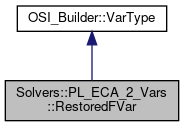
\includegraphics[width=210pt]{class_solvers_1_1_p_l___e_c_a__2___vars_1_1_restored_f_var__inherit__graph}
\end{center}
\end{figure}


Collaboration diagram for Solvers\+:\+:P\+L\+\_\+\+E\+C\+A\+\_\+2\+\_\+\+Vars\+:\+:Restored\+F\+Var\+:\nopagebreak
\begin{figure}[H]
\begin{center}
\leavevmode
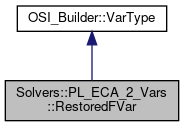
\includegraphics[width=210pt]{class_solvers_1_1_p_l___e_c_a__2___vars_1_1_restored_f_var__coll__graph}
\end{center}
\end{figure}
\subsection*{Public Member Functions}
\begin{DoxyCompactItemize}
\item 
\hyperlink{class_solvers_1_1_p_l___e_c_a__2___vars_1_1_restored_f_var_a1b2057a7d94477eb0f782cab5071de7c}{Restored\+F\+Var} (const \hyperlink{class_restoration_plan}{Restoration\+Plan} \&plan)
\item 
int \hyperlink{class_solvers_1_1_p_l___e_c_a__2___vars_1_1_restored_f_var_a90719c3bd2b7d3bdbafd8c3f01a4b598}{id} (Graph\+\_\+t\+::\+Node t, const \hyperlink{class_restoration_plan_1_1_option}{Restoration\+Plan\+::\+Option} $\ast$option)
\end{DoxyCompactItemize}
\subsection*{Additional Inherited Members}


\subsection{Constructor \& Destructor Documentation}
\mbox{\Hypertarget{class_solvers_1_1_p_l___e_c_a__2___vars_1_1_restored_f_var_a1b2057a7d94477eb0f782cab5071de7c}\label{class_solvers_1_1_p_l___e_c_a__2___vars_1_1_restored_f_var_a1b2057a7d94477eb0f782cab5071de7c}} 
\index{Solvers\+::\+P\+L\+\_\+\+E\+C\+A\+\_\+2\+\_\+\+Vars\+::\+Restored\+F\+Var@{Solvers\+::\+P\+L\+\_\+\+E\+C\+A\+\_\+2\+\_\+\+Vars\+::\+Restored\+F\+Var}!Restored\+F\+Var@{Restored\+F\+Var}}
\index{Restored\+F\+Var@{Restored\+F\+Var}!Solvers\+::\+P\+L\+\_\+\+E\+C\+A\+\_\+2\+\_\+\+Vars\+::\+Restored\+F\+Var@{Solvers\+::\+P\+L\+\_\+\+E\+C\+A\+\_\+2\+\_\+\+Vars\+::\+Restored\+F\+Var}}
\subsubsection{\texorpdfstring{Restored\+F\+Var()}{RestoredFVar()}}
{\footnotesize\ttfamily Solvers\+::\+P\+L\+\_\+\+E\+C\+A\+\_\+2\+\_\+\+Vars\+::\+Restored\+F\+Var\+::\+Restored\+F\+Var (\begin{DoxyParamCaption}\item[{const \hyperlink{class_restoration_plan}{Restoration\+Plan} \&}]{plan }\end{DoxyParamCaption})\hspace{0.3cm}{\ttfamily [inline]}}



\subsection{Member Function Documentation}
\mbox{\Hypertarget{class_solvers_1_1_p_l___e_c_a__2___vars_1_1_restored_f_var_a90719c3bd2b7d3bdbafd8c3f01a4b598}\label{class_solvers_1_1_p_l___e_c_a__2___vars_1_1_restored_f_var_a90719c3bd2b7d3bdbafd8c3f01a4b598}} 
\index{Solvers\+::\+P\+L\+\_\+\+E\+C\+A\+\_\+2\+\_\+\+Vars\+::\+Restored\+F\+Var@{Solvers\+::\+P\+L\+\_\+\+E\+C\+A\+\_\+2\+\_\+\+Vars\+::\+Restored\+F\+Var}!id@{id}}
\index{id@{id}!Solvers\+::\+P\+L\+\_\+\+E\+C\+A\+\_\+2\+\_\+\+Vars\+::\+Restored\+F\+Var@{Solvers\+::\+P\+L\+\_\+\+E\+C\+A\+\_\+2\+\_\+\+Vars\+::\+Restored\+F\+Var}}
\subsubsection{\texorpdfstring{id()}{id()}}
{\footnotesize\ttfamily int Solvers\+::\+P\+L\+\_\+\+E\+C\+A\+\_\+2\+\_\+\+Vars\+::\+Restored\+F\+Var\+::id (\begin{DoxyParamCaption}\item[{Graph\+\_\+t\+::\+Node}]{t,  }\item[{const \hyperlink{class_restoration_plan_1_1_option}{Restoration\+Plan\+::\+Option} $\ast$}]{option }\end{DoxyParamCaption})\hspace{0.3cm}{\ttfamily [inline]}}



The documentation for this class was generated from the following file\+:\begin{DoxyCompactItemize}
\item 
/home/plaiseek/\+Projects/landscape\+\_\+opt\+\_\+cpp/src/solvers/\hyperlink{pl__eca__2_8cpp}{pl\+\_\+eca\+\_\+2.\+cpp}\end{DoxyCompactItemize}

\hypertarget{class_solvers_1_1_p_l___e_c_a__3___vars_1_1_restored_f_var}{}\section{Solvers\+:\+:P\+L\+\_\+\+E\+C\+A\+\_\+3\+\_\+\+Vars\+:\+:Restored\+F\+Var Class Reference}
\label{class_solvers_1_1_p_l___e_c_a__3___vars_1_1_restored_f_var}\index{Solvers\+::\+P\+L\+\_\+\+E\+C\+A\+\_\+3\+\_\+\+Vars\+::\+Restored\+F\+Var@{Solvers\+::\+P\+L\+\_\+\+E\+C\+A\+\_\+3\+\_\+\+Vars\+::\+Restored\+F\+Var}}


Inheritance diagram for Solvers\+:\+:P\+L\+\_\+\+E\+C\+A\+\_\+3\+\_\+\+Vars\+:\+:Restored\+F\+Var\+:\nopagebreak
\begin{figure}[H]
\begin{center}
\leavevmode
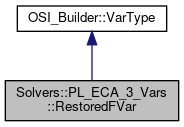
\includegraphics[width=210pt]{class_solvers_1_1_p_l___e_c_a__3___vars_1_1_restored_f_var__inherit__graph}
\end{center}
\end{figure}


Collaboration diagram for Solvers\+:\+:P\+L\+\_\+\+E\+C\+A\+\_\+3\+\_\+\+Vars\+:\+:Restored\+F\+Var\+:\nopagebreak
\begin{figure}[H]
\begin{center}
\leavevmode
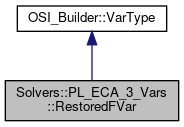
\includegraphics[width=210pt]{class_solvers_1_1_p_l___e_c_a__3___vars_1_1_restored_f_var__coll__graph}
\end{center}
\end{figure}
\subsection*{Public Member Functions}
\begin{DoxyCompactItemize}
\item 
\hyperlink{class_solvers_1_1_p_l___e_c_a__3___vars_1_1_restored_f_var_aaed3e70e43300c1278e832fa7c8fa4b3}{Restored\+F\+Var} (const \hyperlink{class_contraction_result}{Contraction\+Result} \&cr)
\item 
int \hyperlink{class_solvers_1_1_p_l___e_c_a__3___vars_1_1_restored_f_var_a6b81867338d51f2b392aad8b2e795efb}{id} (const \hyperlink{class_restoration_plan_1_1_option}{Restoration\+Plan\+::\+Option} $\ast$option) const
\end{DoxyCompactItemize}
\subsection*{Additional Inherited Members}


\subsection{Constructor \& Destructor Documentation}
\mbox{\Hypertarget{class_solvers_1_1_p_l___e_c_a__3___vars_1_1_restored_f_var_aaed3e70e43300c1278e832fa7c8fa4b3}\label{class_solvers_1_1_p_l___e_c_a__3___vars_1_1_restored_f_var_aaed3e70e43300c1278e832fa7c8fa4b3}} 
\index{Solvers\+::\+P\+L\+\_\+\+E\+C\+A\+\_\+3\+\_\+\+Vars\+::\+Restored\+F\+Var@{Solvers\+::\+P\+L\+\_\+\+E\+C\+A\+\_\+3\+\_\+\+Vars\+::\+Restored\+F\+Var}!Restored\+F\+Var@{Restored\+F\+Var}}
\index{Restored\+F\+Var@{Restored\+F\+Var}!Solvers\+::\+P\+L\+\_\+\+E\+C\+A\+\_\+3\+\_\+\+Vars\+::\+Restored\+F\+Var@{Solvers\+::\+P\+L\+\_\+\+E\+C\+A\+\_\+3\+\_\+\+Vars\+::\+Restored\+F\+Var}}
\subsubsection{\texorpdfstring{Restored\+F\+Var()}{RestoredFVar()}}
{\footnotesize\ttfamily Solvers\+::\+P\+L\+\_\+\+E\+C\+A\+\_\+3\+\_\+\+Vars\+::\+Restored\+F\+Var\+::\+Restored\+F\+Var (\begin{DoxyParamCaption}\item[{const \hyperlink{class_contraction_result}{Contraction\+Result} \&}]{cr }\end{DoxyParamCaption})\hspace{0.3cm}{\ttfamily [inline]}}



\subsection{Member Function Documentation}
\mbox{\Hypertarget{class_solvers_1_1_p_l___e_c_a__3___vars_1_1_restored_f_var_a6b81867338d51f2b392aad8b2e795efb}\label{class_solvers_1_1_p_l___e_c_a__3___vars_1_1_restored_f_var_a6b81867338d51f2b392aad8b2e795efb}} 
\index{Solvers\+::\+P\+L\+\_\+\+E\+C\+A\+\_\+3\+\_\+\+Vars\+::\+Restored\+F\+Var@{Solvers\+::\+P\+L\+\_\+\+E\+C\+A\+\_\+3\+\_\+\+Vars\+::\+Restored\+F\+Var}!id@{id}}
\index{id@{id}!Solvers\+::\+P\+L\+\_\+\+E\+C\+A\+\_\+3\+\_\+\+Vars\+::\+Restored\+F\+Var@{Solvers\+::\+P\+L\+\_\+\+E\+C\+A\+\_\+3\+\_\+\+Vars\+::\+Restored\+F\+Var}}
\subsubsection{\texorpdfstring{id()}{id()}}
{\footnotesize\ttfamily int Solvers\+::\+P\+L\+\_\+\+E\+C\+A\+\_\+3\+\_\+\+Vars\+::\+Restored\+F\+Var\+::id (\begin{DoxyParamCaption}\item[{const \hyperlink{class_restoration_plan_1_1_option}{Restoration\+Plan\+::\+Option} $\ast$}]{option }\end{DoxyParamCaption}) const\hspace{0.3cm}{\ttfamily [inline]}}



The documentation for this class was generated from the following file\+:\begin{DoxyCompactItemize}
\item 
/home/plaiseek/\+Projects/landscape\+\_\+opt\+\_\+cpp/src/solvers/\hyperlink{pl__eca__3_8cpp}{pl\+\_\+eca\+\_\+3.\+cpp}\end{DoxyCompactItemize}

\hypertarget{class_solvers_1_1_p_l___e_c_a__2___vars_1_1_restored_x_var}{}\section{Solvers\+:\+:P\+L\+\_\+\+E\+C\+A\+\_\+2\+\_\+\+Vars\+:\+:Restored\+X\+Var Class Reference}
\label{class_solvers_1_1_p_l___e_c_a__2___vars_1_1_restored_x_var}\index{Solvers\+::\+P\+L\+\_\+\+E\+C\+A\+\_\+2\+\_\+\+Vars\+::\+Restored\+X\+Var@{Solvers\+::\+P\+L\+\_\+\+E\+C\+A\+\_\+2\+\_\+\+Vars\+::\+Restored\+X\+Var}}


Inheritance diagram for Solvers\+:\+:P\+L\+\_\+\+E\+C\+A\+\_\+2\+\_\+\+Vars\+:\+:Restored\+X\+Var\+:\nopagebreak
\begin{figure}[H]
\begin{center}
\leavevmode
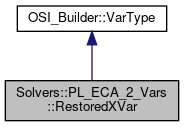
\includegraphics[width=210pt]{class_solvers_1_1_p_l___e_c_a__2___vars_1_1_restored_x_var__inherit__graph}
\end{center}
\end{figure}


Collaboration diagram for Solvers\+:\+:P\+L\+\_\+\+E\+C\+A\+\_\+2\+\_\+\+Vars\+:\+:Restored\+X\+Var\+:\nopagebreak
\begin{figure}[H]
\begin{center}
\leavevmode
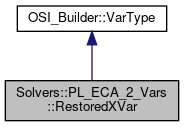
\includegraphics[width=210pt]{class_solvers_1_1_p_l___e_c_a__2___vars_1_1_restored_x_var__coll__graph}
\end{center}
\end{figure}
\subsection*{Public Member Functions}
\begin{DoxyCompactItemize}
\item 
\hyperlink{class_solvers_1_1_p_l___e_c_a__2___vars_1_1_restored_x_var_a682003d690eb9fc6ec1d6ac8056c696b}{Restored\+X\+Var} (const \hyperlink{class_restoration_plan}{Restoration\+Plan} \&plan, int n)
\item 
int \hyperlink{class_solvers_1_1_p_l___e_c_a__2___vars_1_1_restored_x_var_af3514307162d916aee89a45d294c7e3d}{id} (Graph\+\_\+t\+::\+Node t, Graph\+\_\+t\+::\+Arc a, \hyperlink{class_restoration_plan_1_1_option}{Restoration\+Plan\+::\+Option} $\ast$option)
\end{DoxyCompactItemize}
\subsection*{Additional Inherited Members}


\subsection{Constructor \& Destructor Documentation}
\mbox{\Hypertarget{class_solvers_1_1_p_l___e_c_a__2___vars_1_1_restored_x_var_a682003d690eb9fc6ec1d6ac8056c696b}\label{class_solvers_1_1_p_l___e_c_a__2___vars_1_1_restored_x_var_a682003d690eb9fc6ec1d6ac8056c696b}} 
\index{Solvers\+::\+P\+L\+\_\+\+E\+C\+A\+\_\+2\+\_\+\+Vars\+::\+Restored\+X\+Var@{Solvers\+::\+P\+L\+\_\+\+E\+C\+A\+\_\+2\+\_\+\+Vars\+::\+Restored\+X\+Var}!Restored\+X\+Var@{Restored\+X\+Var}}
\index{Restored\+X\+Var@{Restored\+X\+Var}!Solvers\+::\+P\+L\+\_\+\+E\+C\+A\+\_\+2\+\_\+\+Vars\+::\+Restored\+X\+Var@{Solvers\+::\+P\+L\+\_\+\+E\+C\+A\+\_\+2\+\_\+\+Vars\+::\+Restored\+X\+Var}}
\subsubsection{\texorpdfstring{Restored\+X\+Var()}{RestoredXVar()}}
{\footnotesize\ttfamily Solvers\+::\+P\+L\+\_\+\+E\+C\+A\+\_\+2\+\_\+\+Vars\+::\+Restored\+X\+Var\+::\+Restored\+X\+Var (\begin{DoxyParamCaption}\item[{const \hyperlink{class_restoration_plan}{Restoration\+Plan} \&}]{plan,  }\item[{int}]{n }\end{DoxyParamCaption})\hspace{0.3cm}{\ttfamily [inline]}}



\subsection{Member Function Documentation}
\mbox{\Hypertarget{class_solvers_1_1_p_l___e_c_a__2___vars_1_1_restored_x_var_af3514307162d916aee89a45d294c7e3d}\label{class_solvers_1_1_p_l___e_c_a__2___vars_1_1_restored_x_var_af3514307162d916aee89a45d294c7e3d}} 
\index{Solvers\+::\+P\+L\+\_\+\+E\+C\+A\+\_\+2\+\_\+\+Vars\+::\+Restored\+X\+Var@{Solvers\+::\+P\+L\+\_\+\+E\+C\+A\+\_\+2\+\_\+\+Vars\+::\+Restored\+X\+Var}!id@{id}}
\index{id@{id}!Solvers\+::\+P\+L\+\_\+\+E\+C\+A\+\_\+2\+\_\+\+Vars\+::\+Restored\+X\+Var@{Solvers\+::\+P\+L\+\_\+\+E\+C\+A\+\_\+2\+\_\+\+Vars\+::\+Restored\+X\+Var}}
\subsubsection{\texorpdfstring{id()}{id()}}
{\footnotesize\ttfamily int Solvers\+::\+P\+L\+\_\+\+E\+C\+A\+\_\+2\+\_\+\+Vars\+::\+Restored\+X\+Var\+::id (\begin{DoxyParamCaption}\item[{Graph\+\_\+t\+::\+Node}]{t,  }\item[{Graph\+\_\+t\+::\+Arc}]{a,  }\item[{\hyperlink{class_restoration_plan_1_1_option}{Restoration\+Plan\+::\+Option} $\ast$}]{option }\end{DoxyParamCaption})\hspace{0.3cm}{\ttfamily [inline]}}



The documentation for this class was generated from the following file\+:\begin{DoxyCompactItemize}
\item 
/home/plaiseek/\+Projects/landscape\+\_\+opt\+\_\+cpp/src/solvers/\hyperlink{pl__eca__2_8cpp}{pl\+\_\+eca\+\_\+2.\+cpp}\end{DoxyCompactItemize}

\hypertarget{class_solvers_1_1_p_l___e_c_a__3___vars_1_1_restored_x_var}{}\section{Solvers\+:\+:P\+L\+\_\+\+E\+C\+A\+\_\+3\+\_\+\+Vars\+:\+:Restored\+X\+Var Class Reference}
\label{class_solvers_1_1_p_l___e_c_a__3___vars_1_1_restored_x_var}\index{Solvers\+::\+P\+L\+\_\+\+E\+C\+A\+\_\+3\+\_\+\+Vars\+::\+Restored\+X\+Var@{Solvers\+::\+P\+L\+\_\+\+E\+C\+A\+\_\+3\+\_\+\+Vars\+::\+Restored\+X\+Var}}


Inheritance diagram for Solvers\+:\+:P\+L\+\_\+\+E\+C\+A\+\_\+3\+\_\+\+Vars\+:\+:Restored\+X\+Var\+:\nopagebreak
\begin{figure}[H]
\begin{center}
\leavevmode
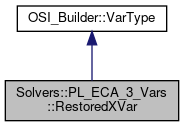
\includegraphics[width=210pt]{class_solvers_1_1_p_l___e_c_a__3___vars_1_1_restored_x_var__inherit__graph}
\end{center}
\end{figure}


Collaboration diagram for Solvers\+:\+:P\+L\+\_\+\+E\+C\+A\+\_\+3\+\_\+\+Vars\+:\+:Restored\+X\+Var\+:\nopagebreak
\begin{figure}[H]
\begin{center}
\leavevmode
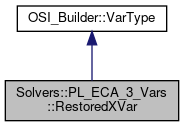
\includegraphics[width=210pt]{class_solvers_1_1_p_l___e_c_a__3___vars_1_1_restored_x_var__coll__graph}
\end{center}
\end{figure}
\subsection*{Public Member Functions}
\begin{DoxyCompactItemize}
\item 
\hyperlink{class_solvers_1_1_p_l___e_c_a__3___vars_1_1_restored_x_var_a3dc06edea3e4cccd9b2500c9135fe3ff}{Restored\+X\+Var} (const \hyperlink{class_contraction_result}{Contraction\+Result} \&cr)
\item 
int \hyperlink{class_solvers_1_1_p_l___e_c_a__3___vars_1_1_restored_x_var_a5359b529bcc8e68b13acedb66b04553b}{id} (Graph\+\_\+t\+::\+Arc a, \hyperlink{class_restoration_plan_1_1_option}{Restoration\+Plan\+::\+Option} $\ast$option) const
\end{DoxyCompactItemize}
\subsection*{Additional Inherited Members}


\subsection{Constructor \& Destructor Documentation}
\mbox{\Hypertarget{class_solvers_1_1_p_l___e_c_a__3___vars_1_1_restored_x_var_a3dc06edea3e4cccd9b2500c9135fe3ff}\label{class_solvers_1_1_p_l___e_c_a__3___vars_1_1_restored_x_var_a3dc06edea3e4cccd9b2500c9135fe3ff}} 
\index{Solvers\+::\+P\+L\+\_\+\+E\+C\+A\+\_\+3\+\_\+\+Vars\+::\+Restored\+X\+Var@{Solvers\+::\+P\+L\+\_\+\+E\+C\+A\+\_\+3\+\_\+\+Vars\+::\+Restored\+X\+Var}!Restored\+X\+Var@{Restored\+X\+Var}}
\index{Restored\+X\+Var@{Restored\+X\+Var}!Solvers\+::\+P\+L\+\_\+\+E\+C\+A\+\_\+3\+\_\+\+Vars\+::\+Restored\+X\+Var@{Solvers\+::\+P\+L\+\_\+\+E\+C\+A\+\_\+3\+\_\+\+Vars\+::\+Restored\+X\+Var}}
\subsubsection{\texorpdfstring{Restored\+X\+Var()}{RestoredXVar()}}
{\footnotesize\ttfamily Solvers\+::\+P\+L\+\_\+\+E\+C\+A\+\_\+3\+\_\+\+Vars\+::\+Restored\+X\+Var\+::\+Restored\+X\+Var (\begin{DoxyParamCaption}\item[{const \hyperlink{class_contraction_result}{Contraction\+Result} \&}]{cr }\end{DoxyParamCaption})\hspace{0.3cm}{\ttfamily [inline]}}



\subsection{Member Function Documentation}
\mbox{\Hypertarget{class_solvers_1_1_p_l___e_c_a__3___vars_1_1_restored_x_var_a5359b529bcc8e68b13acedb66b04553b}\label{class_solvers_1_1_p_l___e_c_a__3___vars_1_1_restored_x_var_a5359b529bcc8e68b13acedb66b04553b}} 
\index{Solvers\+::\+P\+L\+\_\+\+E\+C\+A\+\_\+3\+\_\+\+Vars\+::\+Restored\+X\+Var@{Solvers\+::\+P\+L\+\_\+\+E\+C\+A\+\_\+3\+\_\+\+Vars\+::\+Restored\+X\+Var}!id@{id}}
\index{id@{id}!Solvers\+::\+P\+L\+\_\+\+E\+C\+A\+\_\+3\+\_\+\+Vars\+::\+Restored\+X\+Var@{Solvers\+::\+P\+L\+\_\+\+E\+C\+A\+\_\+3\+\_\+\+Vars\+::\+Restored\+X\+Var}}
\subsubsection{\texorpdfstring{id()}{id()}}
{\footnotesize\ttfamily int Solvers\+::\+P\+L\+\_\+\+E\+C\+A\+\_\+3\+\_\+\+Vars\+::\+Restored\+X\+Var\+::id (\begin{DoxyParamCaption}\item[{Graph\+\_\+t\+::\+Arc}]{a,  }\item[{\hyperlink{class_restoration_plan_1_1_option}{Restoration\+Plan\+::\+Option} $\ast$}]{option }\end{DoxyParamCaption}) const\hspace{0.3cm}{\ttfamily [inline]}}



The documentation for this class was generated from the following file\+:\begin{DoxyCompactItemize}
\item 
/home/plaiseek/\+Projects/landscape\+\_\+opt\+\_\+cpp/src/solvers/\hyperlink{pl__eca__3_8cpp}{pl\+\_\+eca\+\_\+3.\+cpp}\end{DoxyCompactItemize}

\hypertarget{classlemon_1_1_simpler_dijkstra}{}\section{lemon\+:\+:Simpler\+Dijkstra$<$ GR, L\+EN, TR $>$ Class Template Reference}
\label{classlemon_1_1_simpler_dijkstra}\index{lemon\+::\+Simpler\+Dijkstra$<$ G\+R, L\+E\+N, T\+R $>$@{lemon\+::\+Simpler\+Dijkstra$<$ G\+R, L\+E\+N, T\+R $>$}}


A minimalist Dijkstra algorithm class based on Dijkstra.  




{\ttfamily \#include $<$multiplicative\+\_\+dijkstra.\+h$>$}

\subsection*{Public Types}
\begin{DoxyCompactItemize}
\item 
typedef T\+R\+::\+Digraph \hyperlink{classlemon_1_1_simpler_dijkstra_ac19103e2c76d2258f7507dd5921d814d}{Digraph}
\item 
typedef T\+R\+::\+Value \hyperlink{classlemon_1_1_simpler_dijkstra_adbbec2bbc5762ccc02fee8089e30836a}{Value}
\item 
typedef T\+R\+::\+Length\+Map \hyperlink{classlemon_1_1_simpler_dijkstra_adfe5498ef0a7699daf396dd6c4b7dfb6}{Length\+Map}
\item 
typedef T\+R\+::\+Heap\+Cross\+Ref \hyperlink{classlemon_1_1_simpler_dijkstra_ae4c36812930d6292b4154e26b76ea10f}{Heap\+Cross\+Ref}
\item 
typedef T\+R\+::\+Heap \hyperlink{classlemon_1_1_simpler_dijkstra_aafddddfbd1c0c9c054fffa959a2a1a3f}{Heap}
\item 
typedef T\+R\+::\+Operation\+Traits \hyperlink{classlemon_1_1_simpler_dijkstra_a324250f3aac580ddcc57cb2a84d5e9cd}{Operation\+Traits}
\item 
typedef TR \hyperlink{classlemon_1_1_simpler_dijkstra_aba2e25936434ef18b495a05a4b785220}{Traits}
\end{DoxyCompactItemize}
\subsection*{Public Member Functions}
\begin{DoxyCompactItemize}
\item 
\hyperlink{classlemon_1_1_simpler_dijkstra_aafa6d31f7d5de94342454613f321aff8}{Simpler\+Dijkstra} (const \hyperlink{classlemon_1_1_simpler_dijkstra_ac19103e2c76d2258f7507dd5921d814d}{Digraph} \&g, const \hyperlink{classlemon_1_1_simpler_dijkstra_adfe5498ef0a7699daf396dd6c4b7dfb6}{Length\+Map} \&length)
\item 
\hyperlink{classlemon_1_1_simpler_dijkstra_a4f5e5b5fdbdc7bcb61c41cbf6caf4c9f}{$\sim$\+Simpler\+Dijkstra} ()
\item 
void \hyperlink{classlemon_1_1_simpler_dijkstra_a714103f8b8c32f17211bdd0dae12fe4e}{init} (Node s)
\item 
bool \hyperlink{classlemon_1_1_simpler_dijkstra_a5f76dcaec68bd9b4e9df63a32565ebcc}{empty\+Queue} () const
\item 
std\+::pair$<$ typename G\+R\+::\+Node, double $>$ \hyperlink{classlemon_1_1_simpler_dijkstra_a84a7dcefca1d2a82a6af236dc082d77a}{process\+Next\+Node} ()
\end{DoxyCompactItemize}


\subsection{Detailed Description}
\subsubsection*{template$<$typename GR = List\+Digraph, typename L\+EN = typename G\+R\+::template Arc\+Map$<$int$>$, typename TR = Dijkstra\+Default\+Traits$<$\+G\+R,\+L\+E\+N$>$$>$\newline
class lemon\+::\+Simpler\+Dijkstra$<$ G\+R, L\+E\+N, T\+R $>$}

A minimalist Dijkstra algorithm class based on Dijkstra. 


\begin{DoxyTemplParams}{Template Parameters}
{\em GR} & The type of the digraph the algorithm runs on. \\
\hline
{\em L\+EN} & readable arc map that specifies the lengths of the arcs. \\
\hline
{\em TR} & The traits class that defines various types used by the algorithm. By default, it is Dijkstra\+Default\+Traits$<$GR, L\+EN$>$ \\
\hline
\end{DoxyTemplParams}


\subsection{Member Typedef Documentation}
\mbox{\Hypertarget{classlemon_1_1_simpler_dijkstra_ac19103e2c76d2258f7507dd5921d814d}\label{classlemon_1_1_simpler_dijkstra_ac19103e2c76d2258f7507dd5921d814d}} 
\index{lemon\+::\+Simpler\+Dijkstra@{lemon\+::\+Simpler\+Dijkstra}!Digraph@{Digraph}}
\index{Digraph@{Digraph}!lemon\+::\+Simpler\+Dijkstra@{lemon\+::\+Simpler\+Dijkstra}}
\subsubsection{\texorpdfstring{Digraph}{Digraph}}
{\footnotesize\ttfamily template$<$typename GR = List\+Digraph, typename L\+EN = typename G\+R\+::template Arc\+Map$<$int$>$, typename TR = Dijkstra\+Default\+Traits$<$\+G\+R,\+L\+E\+N$>$$>$ \\
typedef T\+R\+::\+Digraph \hyperlink{classlemon_1_1_simpler_dijkstra}{lemon\+::\+Simpler\+Dijkstra}$<$ GR, L\+EN, TR $>$\+::\hyperlink{classlemon_1_1_simpler_dijkstra_ac19103e2c76d2258f7507dd5921d814d}{Digraph}}

\mbox{\Hypertarget{classlemon_1_1_simpler_dijkstra_aafddddfbd1c0c9c054fffa959a2a1a3f}\label{classlemon_1_1_simpler_dijkstra_aafddddfbd1c0c9c054fffa959a2a1a3f}} 
\index{lemon\+::\+Simpler\+Dijkstra@{lemon\+::\+Simpler\+Dijkstra}!Heap@{Heap}}
\index{Heap@{Heap}!lemon\+::\+Simpler\+Dijkstra@{lemon\+::\+Simpler\+Dijkstra}}
\subsubsection{\texorpdfstring{Heap}{Heap}}
{\footnotesize\ttfamily template$<$typename GR = List\+Digraph, typename L\+EN = typename G\+R\+::template Arc\+Map$<$int$>$, typename TR = Dijkstra\+Default\+Traits$<$\+G\+R,\+L\+E\+N$>$$>$ \\
typedef T\+R\+::\+Heap \hyperlink{classlemon_1_1_simpler_dijkstra}{lemon\+::\+Simpler\+Dijkstra}$<$ GR, L\+EN, TR $>$\+::\hyperlink{classlemon_1_1_simpler_dijkstra_aafddddfbd1c0c9c054fffa959a2a1a3f}{Heap}}

\mbox{\Hypertarget{classlemon_1_1_simpler_dijkstra_ae4c36812930d6292b4154e26b76ea10f}\label{classlemon_1_1_simpler_dijkstra_ae4c36812930d6292b4154e26b76ea10f}} 
\index{lemon\+::\+Simpler\+Dijkstra@{lemon\+::\+Simpler\+Dijkstra}!Heap\+Cross\+Ref@{Heap\+Cross\+Ref}}
\index{Heap\+Cross\+Ref@{Heap\+Cross\+Ref}!lemon\+::\+Simpler\+Dijkstra@{lemon\+::\+Simpler\+Dijkstra}}
\subsubsection{\texorpdfstring{Heap\+Cross\+Ref}{HeapCrossRef}}
{\footnotesize\ttfamily template$<$typename GR = List\+Digraph, typename L\+EN = typename G\+R\+::template Arc\+Map$<$int$>$, typename TR = Dijkstra\+Default\+Traits$<$\+G\+R,\+L\+E\+N$>$$>$ \\
typedef T\+R\+::\+Heap\+Cross\+Ref \hyperlink{classlemon_1_1_simpler_dijkstra}{lemon\+::\+Simpler\+Dijkstra}$<$ GR, L\+EN, TR $>$\+::\hyperlink{classlemon_1_1_simpler_dijkstra_ae4c36812930d6292b4154e26b76ea10f}{Heap\+Cross\+Ref}}

\mbox{\Hypertarget{classlemon_1_1_simpler_dijkstra_adfe5498ef0a7699daf396dd6c4b7dfb6}\label{classlemon_1_1_simpler_dijkstra_adfe5498ef0a7699daf396dd6c4b7dfb6}} 
\index{lemon\+::\+Simpler\+Dijkstra@{lemon\+::\+Simpler\+Dijkstra}!Length\+Map@{Length\+Map}}
\index{Length\+Map@{Length\+Map}!lemon\+::\+Simpler\+Dijkstra@{lemon\+::\+Simpler\+Dijkstra}}
\subsubsection{\texorpdfstring{Length\+Map}{LengthMap}}
{\footnotesize\ttfamily template$<$typename GR = List\+Digraph, typename L\+EN = typename G\+R\+::template Arc\+Map$<$int$>$, typename TR = Dijkstra\+Default\+Traits$<$\+G\+R,\+L\+E\+N$>$$>$ \\
typedef T\+R\+::\+Length\+Map \hyperlink{classlemon_1_1_simpler_dijkstra}{lemon\+::\+Simpler\+Dijkstra}$<$ GR, L\+EN, TR $>$\+::\hyperlink{classlemon_1_1_simpler_dijkstra_adfe5498ef0a7699daf396dd6c4b7dfb6}{Length\+Map}}

\mbox{\Hypertarget{classlemon_1_1_simpler_dijkstra_a324250f3aac580ddcc57cb2a84d5e9cd}\label{classlemon_1_1_simpler_dijkstra_a324250f3aac580ddcc57cb2a84d5e9cd}} 
\index{lemon\+::\+Simpler\+Dijkstra@{lemon\+::\+Simpler\+Dijkstra}!Operation\+Traits@{Operation\+Traits}}
\index{Operation\+Traits@{Operation\+Traits}!lemon\+::\+Simpler\+Dijkstra@{lemon\+::\+Simpler\+Dijkstra}}
\subsubsection{\texorpdfstring{Operation\+Traits}{OperationTraits}}
{\footnotesize\ttfamily template$<$typename GR = List\+Digraph, typename L\+EN = typename G\+R\+::template Arc\+Map$<$int$>$, typename TR = Dijkstra\+Default\+Traits$<$\+G\+R,\+L\+E\+N$>$$>$ \\
typedef T\+R\+::\+Operation\+Traits \hyperlink{classlemon_1_1_simpler_dijkstra}{lemon\+::\+Simpler\+Dijkstra}$<$ GR, L\+EN, TR $>$\+::\hyperlink{classlemon_1_1_simpler_dijkstra_a324250f3aac580ddcc57cb2a84d5e9cd}{Operation\+Traits}}

\mbox{\Hypertarget{classlemon_1_1_simpler_dijkstra_aba2e25936434ef18b495a05a4b785220}\label{classlemon_1_1_simpler_dijkstra_aba2e25936434ef18b495a05a4b785220}} 
\index{lemon\+::\+Simpler\+Dijkstra@{lemon\+::\+Simpler\+Dijkstra}!Traits@{Traits}}
\index{Traits@{Traits}!lemon\+::\+Simpler\+Dijkstra@{lemon\+::\+Simpler\+Dijkstra}}
\subsubsection{\texorpdfstring{Traits}{Traits}}
{\footnotesize\ttfamily template$<$typename GR = List\+Digraph, typename L\+EN = typename G\+R\+::template Arc\+Map$<$int$>$, typename TR = Dijkstra\+Default\+Traits$<$\+G\+R,\+L\+E\+N$>$$>$ \\
typedef TR \hyperlink{classlemon_1_1_simpler_dijkstra}{lemon\+::\+Simpler\+Dijkstra}$<$ GR, L\+EN, TR $>$\+::\hyperlink{classlemon_1_1_simpler_dijkstra_aba2e25936434ef18b495a05a4b785220}{Traits}}

\mbox{\Hypertarget{classlemon_1_1_simpler_dijkstra_adbbec2bbc5762ccc02fee8089e30836a}\label{classlemon_1_1_simpler_dijkstra_adbbec2bbc5762ccc02fee8089e30836a}} 
\index{lemon\+::\+Simpler\+Dijkstra@{lemon\+::\+Simpler\+Dijkstra}!Value@{Value}}
\index{Value@{Value}!lemon\+::\+Simpler\+Dijkstra@{lemon\+::\+Simpler\+Dijkstra}}
\subsubsection{\texorpdfstring{Value}{Value}}
{\footnotesize\ttfamily template$<$typename GR = List\+Digraph, typename L\+EN = typename G\+R\+::template Arc\+Map$<$int$>$, typename TR = Dijkstra\+Default\+Traits$<$\+G\+R,\+L\+E\+N$>$$>$ \\
typedef T\+R\+::\+Value \hyperlink{classlemon_1_1_simpler_dijkstra}{lemon\+::\+Simpler\+Dijkstra}$<$ GR, L\+EN, TR $>$\+::\hyperlink{classlemon_1_1_simpler_dijkstra_adbbec2bbc5762ccc02fee8089e30836a}{Value}}



\subsection{Constructor \& Destructor Documentation}
\mbox{\Hypertarget{classlemon_1_1_simpler_dijkstra_aafa6d31f7d5de94342454613f321aff8}\label{classlemon_1_1_simpler_dijkstra_aafa6d31f7d5de94342454613f321aff8}} 
\index{lemon\+::\+Simpler\+Dijkstra@{lemon\+::\+Simpler\+Dijkstra}!Simpler\+Dijkstra@{Simpler\+Dijkstra}}
\index{Simpler\+Dijkstra@{Simpler\+Dijkstra}!lemon\+::\+Simpler\+Dijkstra@{lemon\+::\+Simpler\+Dijkstra}}
\subsubsection{\texorpdfstring{Simpler\+Dijkstra()}{SimplerDijkstra()}}
{\footnotesize\ttfamily template$<$typename GR = List\+Digraph, typename L\+EN = typename G\+R\+::template Arc\+Map$<$int$>$, typename TR = Dijkstra\+Default\+Traits$<$\+G\+R,\+L\+E\+N$>$$>$ \\
\hyperlink{classlemon_1_1_simpler_dijkstra}{lemon\+::\+Simpler\+Dijkstra}$<$ GR, L\+EN, TR $>$\+::\hyperlink{classlemon_1_1_simpler_dijkstra}{Simpler\+Dijkstra} (\begin{DoxyParamCaption}\item[{const \hyperlink{classlemon_1_1_simpler_dijkstra_ac19103e2c76d2258f7507dd5921d814d}{Digraph} \&}]{g,  }\item[{const \hyperlink{classlemon_1_1_simpler_dijkstra_adfe5498ef0a7699daf396dd6c4b7dfb6}{Length\+Map} \&}]{length }\end{DoxyParamCaption})\hspace{0.3cm}{\ttfamily [inline]}}

\mbox{\Hypertarget{classlemon_1_1_simpler_dijkstra_a4f5e5b5fdbdc7bcb61c41cbf6caf4c9f}\label{classlemon_1_1_simpler_dijkstra_a4f5e5b5fdbdc7bcb61c41cbf6caf4c9f}} 
\index{lemon\+::\+Simpler\+Dijkstra@{lemon\+::\+Simpler\+Dijkstra}!````~Simpler\+Dijkstra@{$\sim$\+Simpler\+Dijkstra}}
\index{````~Simpler\+Dijkstra@{$\sim$\+Simpler\+Dijkstra}!lemon\+::\+Simpler\+Dijkstra@{lemon\+::\+Simpler\+Dijkstra}}
\subsubsection{\texorpdfstring{$\sim$\+Simpler\+Dijkstra()}{~SimplerDijkstra()}}
{\footnotesize\ttfamily template$<$typename GR = List\+Digraph, typename L\+EN = typename G\+R\+::template Arc\+Map$<$int$>$, typename TR = Dijkstra\+Default\+Traits$<$\+G\+R,\+L\+E\+N$>$$>$ \\
\hyperlink{classlemon_1_1_simpler_dijkstra}{lemon\+::\+Simpler\+Dijkstra}$<$ GR, L\+EN, TR $>$\+::$\sim$\hyperlink{classlemon_1_1_simpler_dijkstra}{Simpler\+Dijkstra} (\begin{DoxyParamCaption}{ }\end{DoxyParamCaption})\hspace{0.3cm}{\ttfamily [inline]}}



\subsection{Member Function Documentation}
\mbox{\Hypertarget{classlemon_1_1_simpler_dijkstra_a5f76dcaec68bd9b4e9df63a32565ebcc}\label{classlemon_1_1_simpler_dijkstra_a5f76dcaec68bd9b4e9df63a32565ebcc}} 
\index{lemon\+::\+Simpler\+Dijkstra@{lemon\+::\+Simpler\+Dijkstra}!empty\+Queue@{empty\+Queue}}
\index{empty\+Queue@{empty\+Queue}!lemon\+::\+Simpler\+Dijkstra@{lemon\+::\+Simpler\+Dijkstra}}
\subsubsection{\texorpdfstring{empty\+Queue()}{emptyQueue()}}
{\footnotesize\ttfamily template$<$typename GR = List\+Digraph, typename L\+EN = typename G\+R\+::template Arc\+Map$<$int$>$, typename TR = Dijkstra\+Default\+Traits$<$\+G\+R,\+L\+E\+N$>$$>$ \\
bool \hyperlink{classlemon_1_1_simpler_dijkstra}{lemon\+::\+Simpler\+Dijkstra}$<$ GR, L\+EN, TR $>$\+::empty\+Queue (\begin{DoxyParamCaption}{ }\end{DoxyParamCaption}) const\hspace{0.3cm}{\ttfamily [inline]}}

\mbox{\Hypertarget{classlemon_1_1_simpler_dijkstra_a714103f8b8c32f17211bdd0dae12fe4e}\label{classlemon_1_1_simpler_dijkstra_a714103f8b8c32f17211bdd0dae12fe4e}} 
\index{lemon\+::\+Simpler\+Dijkstra@{lemon\+::\+Simpler\+Dijkstra}!init@{init}}
\index{init@{init}!lemon\+::\+Simpler\+Dijkstra@{lemon\+::\+Simpler\+Dijkstra}}
\subsubsection{\texorpdfstring{init()}{init()}}
{\footnotesize\ttfamily template$<$typename GR = List\+Digraph, typename L\+EN = typename G\+R\+::template Arc\+Map$<$int$>$, typename TR = Dijkstra\+Default\+Traits$<$\+G\+R,\+L\+E\+N$>$$>$ \\
void \hyperlink{classlemon_1_1_simpler_dijkstra}{lemon\+::\+Simpler\+Dijkstra}$<$ GR, L\+EN, TR $>$\+::init (\begin{DoxyParamCaption}\item[{Node}]{s }\end{DoxyParamCaption})\hspace{0.3cm}{\ttfamily [inline]}}

\mbox{\Hypertarget{classlemon_1_1_simpler_dijkstra_a84a7dcefca1d2a82a6af236dc082d77a}\label{classlemon_1_1_simpler_dijkstra_a84a7dcefca1d2a82a6af236dc082d77a}} 
\index{lemon\+::\+Simpler\+Dijkstra@{lemon\+::\+Simpler\+Dijkstra}!process\+Next\+Node@{process\+Next\+Node}}
\index{process\+Next\+Node@{process\+Next\+Node}!lemon\+::\+Simpler\+Dijkstra@{lemon\+::\+Simpler\+Dijkstra}}
\subsubsection{\texorpdfstring{process\+Next\+Node()}{processNextNode()}}
{\footnotesize\ttfamily template$<$typename GR = List\+Digraph, typename L\+EN = typename G\+R\+::template Arc\+Map$<$int$>$, typename TR = Dijkstra\+Default\+Traits$<$\+G\+R,\+L\+E\+N$>$$>$ \\
std\+::pair$<$typename G\+R\+::\+Node, double$>$ \hyperlink{classlemon_1_1_simpler_dijkstra}{lemon\+::\+Simpler\+Dijkstra}$<$ GR, L\+EN, TR $>$\+::process\+Next\+Node (\begin{DoxyParamCaption}{ }\end{DoxyParamCaption})\hspace{0.3cm}{\ttfamily [inline]}}



The documentation for this class was generated from the following file\+:\begin{DoxyCompactItemize}
\item 
/home/plaiseek/\+Projects/landscape\+\_\+opt\+\_\+cpp/include/algorithms/\hyperlink{multiplicative__dijkstra_8h}{multiplicative\+\_\+dijkstra.\+h}\end{DoxyCompactItemize}

\hypertarget{class_solution}{}\section{Solution Class Reference}
\label{class_solution}\index{Solution@{Solution}}


{\ttfamily \#include $<$solution.\+hpp$>$}

\subsection*{Public Member Functions}
\begin{DoxyCompactItemize}
\item 
\hyperlink{class_solution_ab52c6ac6bed551f63788a5da6af7becc}{Solution} (const \hyperlink{class_landscape}{Landscape} \&landscape, const \hyperlink{class_restoration_plan}{Restoration\+Plan} \&plan)
\item 
\hyperlink{class_solution_a5d245f7409aacf6ace5e965b7879a580}{$\sim$\+Solution} ()
\item 
const \hyperlink{class_restoration_plan}{Restoration\+Plan} \& \hyperlink{class_solution_a95446a3f6110054a0085a22bee9ce64e}{get\+Plan} () const
\item 
bool \hyperlink{class_solution_af4e5cc99508f729e1866e0c30c7472a0}{contains} (const \hyperlink{class_restoration_plan_1_1_option}{Restoration\+Plan\+::\+Option} $\ast$option) const
\item 
void \hyperlink{class_solution_ac29d6eca7b0755057b82c95610b763c8}{set} (const \hyperlink{class_restoration_plan_1_1_option}{Restoration\+Plan\+::\+Option} $\ast$option, double coef)
\item 
void \hyperlink{class_solution_ab9df5a4126b96e12dcb998cb0c5fc37a}{add} (const \hyperlink{class_restoration_plan_1_1_option}{Restoration\+Plan\+::\+Option} $\ast$option)
\item 
void \hyperlink{class_solution_a4388ef028db3bc8e6fd6a6be0478cedc}{remove} (const \hyperlink{class_restoration_plan_1_1_option}{Restoration\+Plan\+::\+Option} $\ast$option)
\item 
const std\+::map$<$ const \hyperlink{class_restoration_plan_1_1_option}{Restoration\+Plan\+::\+Option} $\ast$, double $>$ \& \hyperlink{class_solution_a4b97ae617451a4e255179ac1e80eb45e}{get\+Option\+Coefs} () const
\item 
void \hyperlink{class_solution_a24101fa88cf1e685abd9652148e4f1fb}{set\+Compute\+Time\+Ms} (int time\+\_\+ms)
\item 
int \hyperlink{class_solution_a7b42da29828c80b924884729cdcd9b43}{get\+Compute\+Time\+Ms} () const
\item 
double \hyperlink{class_solution_ad4f76bea091ec66302df270168e68feb}{get\+Cost} () const
\end{DoxyCompactItemize}
\subsection*{Public Attributes}
\begin{DoxyCompactItemize}
\item 
int \hyperlink{class_solution_ada3534c6614de6c21ed6406ead921ca2}{nb\+\_\+vars}
\item 
int \hyperlink{class_solution_a12d788f2b7fa64050d2e3c0e3f4464f3}{nb\+\_\+constraints}
\item 
double \hyperlink{class_solution_a261a9de1b33f8ec6219a88073aea29e9}{obj}
\end{DoxyCompactItemize}


\subsection{Constructor \& Destructor Documentation}
\mbox{\Hypertarget{class_solution_ab52c6ac6bed551f63788a5da6af7becc}\label{class_solution_ab52c6ac6bed551f63788a5da6af7becc}} 
\index{Solution@{Solution}!Solution@{Solution}}
\index{Solution@{Solution}!Solution@{Solution}}
\subsubsection{\texorpdfstring{Solution()}{Solution()}}
{\footnotesize\ttfamily Solution\+::\+Solution (\begin{DoxyParamCaption}\item[{const \hyperlink{class_landscape}{Landscape} \&}]{landscape,  }\item[{const \hyperlink{class_restoration_plan}{Restoration\+Plan} \&}]{plan }\end{DoxyParamCaption})\hspace{0.3cm}{\ttfamily [inline]}}

\mbox{\Hypertarget{class_solution_a5d245f7409aacf6ace5e965b7879a580}\label{class_solution_a5d245f7409aacf6ace5e965b7879a580}} 
\index{Solution@{Solution}!````~Solution@{$\sim$\+Solution}}
\index{````~Solution@{$\sim$\+Solution}!Solution@{Solution}}
\subsubsection{\texorpdfstring{$\sim$\+Solution()}{~Solution()}}
{\footnotesize\ttfamily Solution\+::$\sim$\+Solution (\begin{DoxyParamCaption}{ }\end{DoxyParamCaption})\hspace{0.3cm}{\ttfamily [inline]}}



\subsection{Member Function Documentation}
\mbox{\Hypertarget{class_solution_ab9df5a4126b96e12dcb998cb0c5fc37a}\label{class_solution_ab9df5a4126b96e12dcb998cb0c5fc37a}} 
\index{Solution@{Solution}!add@{add}}
\index{add@{add}!Solution@{Solution}}
\subsubsection{\texorpdfstring{add()}{add()}}
{\footnotesize\ttfamily void Solution\+::add (\begin{DoxyParamCaption}\item[{const \hyperlink{class_restoration_plan_1_1_option}{Restoration\+Plan\+::\+Option} $\ast$}]{option }\end{DoxyParamCaption})\hspace{0.3cm}{\ttfamily [inline]}}

\mbox{\Hypertarget{class_solution_af4e5cc99508f729e1866e0c30c7472a0}\label{class_solution_af4e5cc99508f729e1866e0c30c7472a0}} 
\index{Solution@{Solution}!contains@{contains}}
\index{contains@{contains}!Solution@{Solution}}
\subsubsection{\texorpdfstring{contains()}{contains()}}
{\footnotesize\ttfamily bool Solution\+::contains (\begin{DoxyParamCaption}\item[{const \hyperlink{class_restoration_plan_1_1_option}{Restoration\+Plan\+::\+Option} $\ast$}]{option }\end{DoxyParamCaption}) const\hspace{0.3cm}{\ttfamily [inline]}}

\mbox{\Hypertarget{class_solution_a7b42da29828c80b924884729cdcd9b43}\label{class_solution_a7b42da29828c80b924884729cdcd9b43}} 
\index{Solution@{Solution}!get\+Compute\+Time\+Ms@{get\+Compute\+Time\+Ms}}
\index{get\+Compute\+Time\+Ms@{get\+Compute\+Time\+Ms}!Solution@{Solution}}
\subsubsection{\texorpdfstring{get\+Compute\+Time\+Ms()}{getComputeTimeMs()}}
{\footnotesize\ttfamily int Solution\+::get\+Compute\+Time\+Ms (\begin{DoxyParamCaption}{ }\end{DoxyParamCaption}) const\hspace{0.3cm}{\ttfamily [inline]}}

\mbox{\Hypertarget{class_solution_ad4f76bea091ec66302df270168e68feb}\label{class_solution_ad4f76bea091ec66302df270168e68feb}} 
\index{Solution@{Solution}!get\+Cost@{get\+Cost}}
\index{get\+Cost@{get\+Cost}!Solution@{Solution}}
\subsubsection{\texorpdfstring{get\+Cost()}{getCost()}}
{\footnotesize\ttfamily double Solution\+::get\+Cost (\begin{DoxyParamCaption}{ }\end{DoxyParamCaption}) const\hspace{0.3cm}{\ttfamily [inline]}}

\mbox{\Hypertarget{class_solution_a4b97ae617451a4e255179ac1e80eb45e}\label{class_solution_a4b97ae617451a4e255179ac1e80eb45e}} 
\index{Solution@{Solution}!get\+Option\+Coefs@{get\+Option\+Coefs}}
\index{get\+Option\+Coefs@{get\+Option\+Coefs}!Solution@{Solution}}
\subsubsection{\texorpdfstring{get\+Option\+Coefs()}{getOptionCoefs()}}
{\footnotesize\ttfamily const std\+::map$<$const \hyperlink{class_restoration_plan_1_1_option}{Restoration\+Plan\+::\+Option}$\ast$, double$>$\& Solution\+::get\+Option\+Coefs (\begin{DoxyParamCaption}{ }\end{DoxyParamCaption}) const\hspace{0.3cm}{\ttfamily [inline]}}

\mbox{\Hypertarget{class_solution_a95446a3f6110054a0085a22bee9ce64e}\label{class_solution_a95446a3f6110054a0085a22bee9ce64e}} 
\index{Solution@{Solution}!get\+Plan@{get\+Plan}}
\index{get\+Plan@{get\+Plan}!Solution@{Solution}}
\subsubsection{\texorpdfstring{get\+Plan()}{getPlan()}}
{\footnotesize\ttfamily const \hyperlink{class_restoration_plan}{Restoration\+Plan}\& Solution\+::get\+Plan (\begin{DoxyParamCaption}{ }\end{DoxyParamCaption}) const\hspace{0.3cm}{\ttfamily [inline]}}

\mbox{\Hypertarget{class_solution_a4388ef028db3bc8e6fd6a6be0478cedc}\label{class_solution_a4388ef028db3bc8e6fd6a6be0478cedc}} 
\index{Solution@{Solution}!remove@{remove}}
\index{remove@{remove}!Solution@{Solution}}
\subsubsection{\texorpdfstring{remove()}{remove()}}
{\footnotesize\ttfamily void Solution\+::remove (\begin{DoxyParamCaption}\item[{const \hyperlink{class_restoration_plan_1_1_option}{Restoration\+Plan\+::\+Option} $\ast$}]{option }\end{DoxyParamCaption})\hspace{0.3cm}{\ttfamily [inline]}}

\mbox{\Hypertarget{class_solution_ac29d6eca7b0755057b82c95610b763c8}\label{class_solution_ac29d6eca7b0755057b82c95610b763c8}} 
\index{Solution@{Solution}!set@{set}}
\index{set@{set}!Solution@{Solution}}
\subsubsection{\texorpdfstring{set()}{set()}}
{\footnotesize\ttfamily void Solution\+::set (\begin{DoxyParamCaption}\item[{const \hyperlink{class_restoration_plan_1_1_option}{Restoration\+Plan\+::\+Option} $\ast$}]{option,  }\item[{double}]{coef }\end{DoxyParamCaption})\hspace{0.3cm}{\ttfamily [inline]}}

\mbox{\Hypertarget{class_solution_a24101fa88cf1e685abd9652148e4f1fb}\label{class_solution_a24101fa88cf1e685abd9652148e4f1fb}} 
\index{Solution@{Solution}!set\+Compute\+Time\+Ms@{set\+Compute\+Time\+Ms}}
\index{set\+Compute\+Time\+Ms@{set\+Compute\+Time\+Ms}!Solution@{Solution}}
\subsubsection{\texorpdfstring{set\+Compute\+Time\+Ms()}{setComputeTimeMs()}}
{\footnotesize\ttfamily void Solution\+::set\+Compute\+Time\+Ms (\begin{DoxyParamCaption}\item[{int}]{time\+\_\+ms }\end{DoxyParamCaption})\hspace{0.3cm}{\ttfamily [inline]}}



\subsection{Member Data Documentation}
\mbox{\Hypertarget{class_solution_a12d788f2b7fa64050d2e3c0e3f4464f3}\label{class_solution_a12d788f2b7fa64050d2e3c0e3f4464f3}} 
\index{Solution@{Solution}!nb\+\_\+constraints@{nb\+\_\+constraints}}
\index{nb\+\_\+constraints@{nb\+\_\+constraints}!Solution@{Solution}}
\subsubsection{\texorpdfstring{nb\+\_\+constraints}{nb\_constraints}}
{\footnotesize\ttfamily int Solution\+::nb\+\_\+constraints}

\mbox{\Hypertarget{class_solution_ada3534c6614de6c21ed6406ead921ca2}\label{class_solution_ada3534c6614de6c21ed6406ead921ca2}} 
\index{Solution@{Solution}!nb\+\_\+vars@{nb\+\_\+vars}}
\index{nb\+\_\+vars@{nb\+\_\+vars}!Solution@{Solution}}
\subsubsection{\texorpdfstring{nb\+\_\+vars}{nb\_vars}}
{\footnotesize\ttfamily int Solution\+::nb\+\_\+vars}

\mbox{\Hypertarget{class_solution_a261a9de1b33f8ec6219a88073aea29e9}\label{class_solution_a261a9de1b33f8ec6219a88073aea29e9}} 
\index{Solution@{Solution}!obj@{obj}}
\index{obj@{obj}!Solution@{Solution}}
\subsubsection{\texorpdfstring{obj}{obj}}
{\footnotesize\ttfamily double Solution\+::obj}



The documentation for this class was generated from the following file\+:\begin{DoxyCompactItemize}
\item 
/home/plaiseek/\+Projects/landscape\+\_\+opt\+\_\+cpp/include/solvers/concept/\hyperlink{solution_8hpp}{solution.\+hpp}\end{DoxyCompactItemize}

\hypertarget{classconcepts_1_1_solver}{}\section{concepts\+:\+:Solver Class Reference}
\label{classconcepts_1_1_solver}\index{concepts\+::\+Solver@{concepts\+::\+Solver}}


{\ttfamily \#include $<$solver.\+hpp$>$}



Inheritance diagram for concepts\+:\+:Solver\+:\nopagebreak
\begin{figure}[H]
\begin{center}
\leavevmode
\includegraphics[width=343pt]{classconcepts_1_1_solver__inherit__graph}
\end{center}
\end{figure}
\subsection*{Classes}
\begin{DoxyCompactItemize}
\item 
class \hyperlink{classconcepts_1_1_solver_1_1_double_param}{Double\+Param}
\item 
class \hyperlink{classconcepts_1_1_solver_1_1_int_param}{Int\+Param}
\item 
class \hyperlink{classconcepts_1_1_solver_1_1_param}{Param}
\end{DoxyCompactItemize}
\subsection*{Public Member Functions}
\begin{DoxyCompactItemize}
\item 
virtual \hyperlink{classconcepts_1_1_solver_a550134cf412d2c1c1b8c6eed1a477090}{$\sim$\+Solver} ()
\item 
bool \hyperlink{classconcepts_1_1_solver_a2158cd44bcaa736d828a1dcb49058db0}{set\+Param} (std\+::string \hyperlink{classconcepts_1_1_solver_ab995568318a506446228f45cab2fcce7}{name}, const char $\ast$arg)
\item 
std\+::list$<$ std\+::string $>$ $\ast$ \hyperlink{classconcepts_1_1_solver_a65cee6a06fd6c1439f3c17fb7e7fb42c}{get\+Param\+List} () const
\item 
virtual \hyperlink{class_solution}{Solution} $\ast$ \hyperlink{classconcepts_1_1_solver_af323ad29df1e7b87facd7dc007568c80}{solve} (const \hyperlink{class_landscape}{Landscape} \&landscape, const \hyperlink{class_restoration_plan}{Restoration\+Plan} \&plan, const double B) const =0
\item 
virtual const std\+::string \hyperlink{classconcepts_1_1_solver_ab995568318a506446228f45cab2fcce7}{name} () const =0
\item 
std\+::string \hyperlink{classconcepts_1_1_solver_a3f9ca298d2c2ccaa4e1c8337866b8021}{to\+String} () const
\end{DoxyCompactItemize}
\subsection*{Protected Attributes}
\begin{DoxyCompactItemize}
\item 
std\+::map$<$ std\+::string, \hyperlink{classconcepts_1_1_solver_1_1_param}{Param} $\ast$ $>$ \hyperlink{classconcepts_1_1_solver_a6b85828f79e693cba963f2fc98f7edd2}{params}
\end{DoxyCompactItemize}


\subsection{Constructor \& Destructor Documentation}
\mbox{\Hypertarget{classconcepts_1_1_solver_a550134cf412d2c1c1b8c6eed1a477090}\label{classconcepts_1_1_solver_a550134cf412d2c1c1b8c6eed1a477090}} 
\index{concepts\+::\+Solver@{concepts\+::\+Solver}!````~Solver@{$\sim$\+Solver}}
\index{````~Solver@{$\sim$\+Solver}!concepts\+::\+Solver@{concepts\+::\+Solver}}
\subsubsection{\texorpdfstring{$\sim$\+Solver()}{~Solver()}}
{\footnotesize\ttfamily virtual concepts\+::\+Solver\+::$\sim$\+Solver (\begin{DoxyParamCaption}{ }\end{DoxyParamCaption})\hspace{0.3cm}{\ttfamily [inline]}, {\ttfamily [virtual]}}



\subsection{Member Function Documentation}
\mbox{\Hypertarget{classconcepts_1_1_solver_a65cee6a06fd6c1439f3c17fb7e7fb42c}\label{classconcepts_1_1_solver_a65cee6a06fd6c1439f3c17fb7e7fb42c}} 
\index{concepts\+::\+Solver@{concepts\+::\+Solver}!get\+Param\+List@{get\+Param\+List}}
\index{get\+Param\+List@{get\+Param\+List}!concepts\+::\+Solver@{concepts\+::\+Solver}}
\subsubsection{\texorpdfstring{get\+Param\+List()}{getParamList()}}
{\footnotesize\ttfamily std\+::list$<$std\+::string$>$$\ast$ concepts\+::\+Solver\+::get\+Param\+List (\begin{DoxyParamCaption}{ }\end{DoxyParamCaption}) const\hspace{0.3cm}{\ttfamily [inline]}}

\mbox{\Hypertarget{classconcepts_1_1_solver_ab995568318a506446228f45cab2fcce7}\label{classconcepts_1_1_solver_ab995568318a506446228f45cab2fcce7}} 
\index{concepts\+::\+Solver@{concepts\+::\+Solver}!name@{name}}
\index{name@{name}!concepts\+::\+Solver@{concepts\+::\+Solver}}
\subsubsection{\texorpdfstring{name()}{name()}}
{\footnotesize\ttfamily virtual const std\+::string concepts\+::\+Solver\+::name (\begin{DoxyParamCaption}{ }\end{DoxyParamCaption}) const\hspace{0.3cm}{\ttfamily [pure virtual]}}



Implemented in \hyperlink{class_p_l___e_c_a___solver_a4cbbcbfd62d91dacb448470456ac57c7}{P\+L\+\_\+\+E\+C\+A\+\_\+\+Solver}, \hyperlink{class_solvers_1_1_p_l___e_c_a__3_ac265db86ca64eb34ba5370e905686a21}{Solvers\+::\+P\+L\+\_\+\+E\+C\+A\+\_\+3}, \hyperlink{class_solvers_1_1_p_l___e_c_a__2_ab9879a904a2545d929bd2956f23fa1aa}{Solvers\+::\+P\+L\+\_\+\+E\+C\+A\+\_\+2}, \hyperlink{class_solvers_1_1_randomized___rounding___e_c_a_aa9ae623007f23dbd73d367649021c8a9}{Solvers\+::\+Randomized\+\_\+\+Rounding\+\_\+\+E\+CA}, \hyperlink{class_solvers_1_1_naive___e_c_a___dec_a171d5188c9901c251c57efdc9c8b954b}{Solvers\+::\+Naive\+\_\+\+E\+C\+A\+\_\+\+Dec}, \hyperlink{class_solvers_1_1_naive___e_c_a___inc_ace6070af722e226fcd2f9b746cc12944}{Solvers\+::\+Naive\+\_\+\+E\+C\+A\+\_\+\+Inc}, \hyperlink{class_solvers_1_1_glutton___e_c_a___dec_a2990dbcfecba9673d4bbae331aee1a04}{Solvers\+::\+Glutton\+\_\+\+E\+C\+A\+\_\+\+Dec}, \hyperlink{class_solvers_1_1_glutton___e_c_a___inc_afda6b975b3a066aa76711730e5fa2f48}{Solvers\+::\+Glutton\+\_\+\+E\+C\+A\+\_\+\+Inc}, and \hyperlink{class_solvers_1_1_bogo_a496539bab5a74757fe6d50e78e0a641f}{Solvers\+::\+Bogo}.

\mbox{\Hypertarget{classconcepts_1_1_solver_a2158cd44bcaa736d828a1dcb49058db0}\label{classconcepts_1_1_solver_a2158cd44bcaa736d828a1dcb49058db0}} 
\index{concepts\+::\+Solver@{concepts\+::\+Solver}!set\+Param@{set\+Param}}
\index{set\+Param@{set\+Param}!concepts\+::\+Solver@{concepts\+::\+Solver}}
\subsubsection{\texorpdfstring{set\+Param()}{setParam()}}
{\footnotesize\ttfamily bool concepts\+::\+Solver\+::set\+Param (\begin{DoxyParamCaption}\item[{std\+::string}]{name,  }\item[{const char $\ast$}]{arg }\end{DoxyParamCaption})\hspace{0.3cm}{\ttfamily [inline]}}

\mbox{\Hypertarget{classconcepts_1_1_solver_af323ad29df1e7b87facd7dc007568c80}\label{classconcepts_1_1_solver_af323ad29df1e7b87facd7dc007568c80}} 
\index{concepts\+::\+Solver@{concepts\+::\+Solver}!solve@{solve}}
\index{solve@{solve}!concepts\+::\+Solver@{concepts\+::\+Solver}}
\subsubsection{\texorpdfstring{solve()}{solve()}}
{\footnotesize\ttfamily virtual \hyperlink{class_solution}{Solution}$\ast$ concepts\+::\+Solver\+::solve (\begin{DoxyParamCaption}\item[{const \hyperlink{class_landscape}{Landscape} \&}]{landscape,  }\item[{const \hyperlink{class_restoration_plan}{Restoration\+Plan} \&}]{plan,  }\item[{const double}]{B }\end{DoxyParamCaption}) const\hspace{0.3cm}{\ttfamily [pure virtual]}}



Implemented in \hyperlink{class_p_l___e_c_a___solver_a7fe728bb23be76b4aa51e669b73ee10d}{P\+L\+\_\+\+E\+C\+A\+\_\+\+Solver}, \hyperlink{class_solvers_1_1_p_l___e_c_a__3_ae296efd0061d2fbf478732bc9c280202}{Solvers\+::\+P\+L\+\_\+\+E\+C\+A\+\_\+3}, \hyperlink{class_solvers_1_1_p_l___e_c_a__2_a07601fa43e0c530e7a66b1532a9e96a6}{Solvers\+::\+P\+L\+\_\+\+E\+C\+A\+\_\+2}, \hyperlink{class_solvers_1_1_randomized___rounding___e_c_a_a2b2c1f0da1e047a5add3fd1bb5e6f0e8}{Solvers\+::\+Randomized\+\_\+\+Rounding\+\_\+\+E\+CA}, \hyperlink{class_solvers_1_1_naive___e_c_a___dec_a51e13c5f7dac3c937f1a006c8b651657}{Solvers\+::\+Naive\+\_\+\+E\+C\+A\+\_\+\+Dec}, \hyperlink{class_solvers_1_1_naive___e_c_a___inc_af0830eeb54be59ae2f363a32f38cee0c}{Solvers\+::\+Naive\+\_\+\+E\+C\+A\+\_\+\+Inc}, \hyperlink{class_solvers_1_1_glutton___e_c_a___dec_a6b7078518779722dfaed6b1b1a9ba502}{Solvers\+::\+Glutton\+\_\+\+E\+C\+A\+\_\+\+Dec}, \hyperlink{class_solvers_1_1_glutton___e_c_a___inc_a12c872bf34761d875649f3e029dbc952}{Solvers\+::\+Glutton\+\_\+\+E\+C\+A\+\_\+\+Inc}, and \hyperlink{class_solvers_1_1_bogo_a094c019a0efda929bd2369d2a47256f6}{Solvers\+::\+Bogo}.

\mbox{\Hypertarget{classconcepts_1_1_solver_a3f9ca298d2c2ccaa4e1c8337866b8021}\label{classconcepts_1_1_solver_a3f9ca298d2c2ccaa4e1c8337866b8021}} 
\index{concepts\+::\+Solver@{concepts\+::\+Solver}!to\+String@{to\+String}}
\index{to\+String@{to\+String}!concepts\+::\+Solver@{concepts\+::\+Solver}}
\subsubsection{\texorpdfstring{to\+String()}{toString()}}
{\footnotesize\ttfamily std\+::string concepts\+::\+Solver\+::to\+String (\begin{DoxyParamCaption}{ }\end{DoxyParamCaption}) const\hspace{0.3cm}{\ttfamily [inline]}}



\subsection{Member Data Documentation}
\mbox{\Hypertarget{classconcepts_1_1_solver_a6b85828f79e693cba963f2fc98f7edd2}\label{classconcepts_1_1_solver_a6b85828f79e693cba963f2fc98f7edd2}} 
\index{concepts\+::\+Solver@{concepts\+::\+Solver}!params@{params}}
\index{params@{params}!concepts\+::\+Solver@{concepts\+::\+Solver}}
\subsubsection{\texorpdfstring{params}{params}}
{\footnotesize\ttfamily std\+::map$<$std\+::string, \hyperlink{classconcepts_1_1_solver_1_1_param}{Param}$\ast$$>$ concepts\+::\+Solver\+::params\hspace{0.3cm}{\ttfamily [protected]}}



The documentation for this class was generated from the following file\+:\begin{DoxyCompactItemize}
\item 
/home/plaiseek/\+Projects/landscape\+\_\+opt\+\_\+cpp/include/solvers/concept/\hyperlink{solver_8hpp}{solver.\+hpp}\end{DoxyCompactItemize}

\hypertarget{class_std_landscape_parser}{}\section{Std\+Landscape\+Parser Class Reference}
\label{class_std_landscape_parser}\index{Std\+Landscape\+Parser@{Std\+Landscape\+Parser}}


{\ttfamily \#include $<$std\+\_\+landscape\+\_\+parser.\+hpp$>$}



Inheritance diagram for Std\+Landscape\+Parser\+:\nopagebreak
\begin{figure}[H]
\begin{center}
\leavevmode
\includegraphics[width=236pt]{class_std_landscape_parser__inherit__graph}
\end{center}
\end{figure}


Collaboration diagram for Std\+Landscape\+Parser\+:\nopagebreak
\begin{figure}[H]
\begin{center}
\leavevmode
\includegraphics[width=236pt]{class_std_landscape_parser__coll__graph}
\end{center}
\end{figure}
\subsection*{Public Member Functions}
\begin{DoxyCompactItemize}
\item 
\hyperlink{class_std_landscape_parser_a458a4a8dd2cacfe0e708f8632dbbf2ff}{$\sim$\+Std\+Landscape\+Parser} ()
\item 
\hyperlink{class_landscape}{Landscape} $\ast$ \hyperlink{class_std_landscape_parser_a73c807c756f6f6a90d23d95d91a4e700}{parse} (const std\+::filesystem\+::path file\+\_\+name)
\item 
void \hyperlink{class_std_landscape_parser_aa899b09850676bac3abdc04d25882e86}{write} (const \hyperlink{class_landscape}{Landscape} \&landscape, const std\+::filesystem\+::path output, const std\+::string name, bool use\+\_\+range\+\_\+ids=true)
\end{DoxyCompactItemize}
\subsection*{Static Public Member Functions}
\begin{DoxyCompactItemize}
\item 
static \hyperlink{class_std_landscape_parser}{Std\+Landscape\+Parser} \& \hyperlink{class_std_landscape_parser_a849d9a5edb03a7748e19dbcef83b9c1c}{get} () noexcept
\end{DoxyCompactItemize}
\subsection*{Additional Inherited Members}


\subsection{Constructor \& Destructor Documentation}
\mbox{\Hypertarget{class_std_landscape_parser_a458a4a8dd2cacfe0e708f8632dbbf2ff}\label{class_std_landscape_parser_a458a4a8dd2cacfe0e708f8632dbbf2ff}} 
\index{Std\+Landscape\+Parser@{Std\+Landscape\+Parser}!````~Std\+Landscape\+Parser@{$\sim$\+Std\+Landscape\+Parser}}
\index{````~Std\+Landscape\+Parser@{$\sim$\+Std\+Landscape\+Parser}!Std\+Landscape\+Parser@{Std\+Landscape\+Parser}}
\subsubsection{\texorpdfstring{$\sim$\+Std\+Landscape\+Parser()}{~StdLandscapeParser()}}
{\footnotesize\ttfamily Std\+Landscape\+Parser\+::$\sim$\+Std\+Landscape\+Parser (\begin{DoxyParamCaption}{ }\end{DoxyParamCaption})}



\subsection{Member Function Documentation}
\mbox{\Hypertarget{class_std_landscape_parser_a849d9a5edb03a7748e19dbcef83b9c1c}\label{class_std_landscape_parser_a849d9a5edb03a7748e19dbcef83b9c1c}} 
\index{Std\+Landscape\+Parser@{Std\+Landscape\+Parser}!get@{get}}
\index{get@{get}!Std\+Landscape\+Parser@{Std\+Landscape\+Parser}}
\subsubsection{\texorpdfstring{get()}{get()}}
{\footnotesize\ttfamily static \hyperlink{class_std_landscape_parser}{Std\+Landscape\+Parser}\& Std\+Landscape\+Parser\+::get (\begin{DoxyParamCaption}{ }\end{DoxyParamCaption})\hspace{0.3cm}{\ttfamily [inline]}, {\ttfamily [static]}, {\ttfamily [noexcept]}}

\mbox{\Hypertarget{class_std_landscape_parser_a73c807c756f6f6a90d23d95d91a4e700}\label{class_std_landscape_parser_a73c807c756f6f6a90d23d95d91a4e700}} 
\index{Std\+Landscape\+Parser@{Std\+Landscape\+Parser}!parse@{parse}}
\index{parse@{parse}!Std\+Landscape\+Parser@{Std\+Landscape\+Parser}}
\subsubsection{\texorpdfstring{parse()}{parse()}}
{\footnotesize\ttfamily \hyperlink{class_landscape}{Landscape} $\ast$ Std\+Landscape\+Parser\+::parse (\begin{DoxyParamCaption}\item[{const std\+::filesystem\+::path}]{file\+\_\+name }\end{DoxyParamCaption})\hspace{0.3cm}{\ttfamily [virtual]}}



Implements \hyperlink{classconcepts_1_1_parser_ac5e6fbf08f6d462695c946647aafb2ce}{concepts\+::\+Parser$<$ Landscape $>$}.

\mbox{\Hypertarget{class_std_landscape_parser_aa899b09850676bac3abdc04d25882e86}\label{class_std_landscape_parser_aa899b09850676bac3abdc04d25882e86}} 
\index{Std\+Landscape\+Parser@{Std\+Landscape\+Parser}!write@{write}}
\index{write@{write}!Std\+Landscape\+Parser@{Std\+Landscape\+Parser}}
\subsubsection{\texorpdfstring{write()}{write()}}
{\footnotesize\ttfamily void Std\+Landscape\+Parser\+::write (\begin{DoxyParamCaption}\item[{const \hyperlink{class_landscape}{Landscape} \&}]{landscape,  }\item[{const std\+::filesystem\+::path}]{output,  }\item[{const std\+::string}]{name,  }\item[{bool}]{use\+\_\+range\+\_\+ids = {\ttfamily true} }\end{DoxyParamCaption})}



The documentation for this class was generated from the following files\+:\begin{DoxyCompactItemize}
\item 
/home/plaiseek/\+Projects/landscape\+\_\+opt\+\_\+cpp/include/parsers/\hyperlink{std__landscape__parser_8hpp}{std\+\_\+landscape\+\_\+parser.\+hpp}\item 
/home/plaiseek/\+Projects/landscape\+\_\+opt\+\_\+cpp/src/parsers/\hyperlink{std__landscape__parser_8cpp}{std\+\_\+landscape\+\_\+parser.\+cpp}\end{DoxyCompactItemize}

\hypertarget{class_std_restoration_plan_parser}{}\section{Std\+Restoration\+Plan\+Parser Class Reference}
\label{class_std_restoration_plan_parser}\index{Std\+Restoration\+Plan\+Parser@{Std\+Restoration\+Plan\+Parser}}


{\ttfamily \#include $<$std\+\_\+restoration\+\_\+plan\+\_\+parser.\+hpp$>$}



Inheritance diagram for Std\+Restoration\+Plan\+Parser\+:\nopagebreak
\begin{figure}[H]
\begin{center}
\leavevmode
\includegraphics[width=230pt]{class_std_restoration_plan_parser__inherit__graph}
\end{center}
\end{figure}


Collaboration diagram for Std\+Restoration\+Plan\+Parser\+:\nopagebreak
\begin{figure}[H]
\begin{center}
\leavevmode
\includegraphics[width=230pt]{class_std_restoration_plan_parser__coll__graph}
\end{center}
\end{figure}
\subsection*{Public Member Functions}
\begin{DoxyCompactItemize}
\item 
\hyperlink{class_std_restoration_plan_parser_ab8af49e4d1b8fa2490b454e71b42ee10}{Std\+Restoration\+Plan\+Parser} (const \hyperlink{class_landscape}{Landscape} \&l)
\item 
\hyperlink{class_std_restoration_plan_parser_a489cfc5395301d3d32c00a3409ddd10d}{$\sim$\+Std\+Restoration\+Plan\+Parser} ()
\item 
\hyperlink{class_restoration_plan}{Restoration\+Plan} $\ast$ \hyperlink{class_std_restoration_plan_parser_aa9156823445695123f32e2eb232a3509}{parse} (std\+::filesystem\+::path file\+\_\+path)
\item 
bool \hyperlink{class_std_restoration_plan_parser_a988b830911043a737c889971a746f13d}{write} (const \hyperlink{class_restoration_plan}{Restoration\+Plan} \&plan, const std\+::filesystem\+::path output, const std\+::string name, bool use\+\_\+range\+\_\+ids=true)
\end{DoxyCompactItemize}
\subsection*{Additional Inherited Members}


\subsection{Constructor \& Destructor Documentation}
\mbox{\Hypertarget{class_std_restoration_plan_parser_ab8af49e4d1b8fa2490b454e71b42ee10}\label{class_std_restoration_plan_parser_ab8af49e4d1b8fa2490b454e71b42ee10}} 
\index{Std\+Restoration\+Plan\+Parser@{Std\+Restoration\+Plan\+Parser}!Std\+Restoration\+Plan\+Parser@{Std\+Restoration\+Plan\+Parser}}
\index{Std\+Restoration\+Plan\+Parser@{Std\+Restoration\+Plan\+Parser}!Std\+Restoration\+Plan\+Parser@{Std\+Restoration\+Plan\+Parser}}
\subsubsection{\texorpdfstring{Std\+Restoration\+Plan\+Parser()}{StdRestorationPlanParser()}}
{\footnotesize\ttfamily Std\+Restoration\+Plan\+Parser\+::\+Std\+Restoration\+Plan\+Parser (\begin{DoxyParamCaption}\item[{const \hyperlink{class_landscape}{Landscape} \&}]{l }\end{DoxyParamCaption})}

\mbox{\Hypertarget{class_std_restoration_plan_parser_a489cfc5395301d3d32c00a3409ddd10d}\label{class_std_restoration_plan_parser_a489cfc5395301d3d32c00a3409ddd10d}} 
\index{Std\+Restoration\+Plan\+Parser@{Std\+Restoration\+Plan\+Parser}!````~Std\+Restoration\+Plan\+Parser@{$\sim$\+Std\+Restoration\+Plan\+Parser}}
\index{````~Std\+Restoration\+Plan\+Parser@{$\sim$\+Std\+Restoration\+Plan\+Parser}!Std\+Restoration\+Plan\+Parser@{Std\+Restoration\+Plan\+Parser}}
\subsubsection{\texorpdfstring{$\sim$\+Std\+Restoration\+Plan\+Parser()}{~StdRestorationPlanParser()}}
{\footnotesize\ttfamily Std\+Restoration\+Plan\+Parser\+::$\sim$\+Std\+Restoration\+Plan\+Parser (\begin{DoxyParamCaption}{ }\end{DoxyParamCaption})}



\subsection{Member Function Documentation}
\mbox{\Hypertarget{class_std_restoration_plan_parser_aa9156823445695123f32e2eb232a3509}\label{class_std_restoration_plan_parser_aa9156823445695123f32e2eb232a3509}} 
\index{Std\+Restoration\+Plan\+Parser@{Std\+Restoration\+Plan\+Parser}!parse@{parse}}
\index{parse@{parse}!Std\+Restoration\+Plan\+Parser@{Std\+Restoration\+Plan\+Parser}}
\subsubsection{\texorpdfstring{parse()}{parse()}}
{\footnotesize\ttfamily \hyperlink{class_restoration_plan}{Restoration\+Plan} $\ast$ Std\+Restoration\+Plan\+Parser\+::parse (\begin{DoxyParamCaption}\item[{std\+::filesystem\+::path}]{file\+\_\+path }\end{DoxyParamCaption})\hspace{0.3cm}{\ttfamily [virtual]}}



Implements \hyperlink{classconcepts_1_1_parser_ac5e6fbf08f6d462695c946647aafb2ce}{concepts\+::\+Parser$<$ Restoration\+Plan $>$}.

\mbox{\Hypertarget{class_std_restoration_plan_parser_a988b830911043a737c889971a746f13d}\label{class_std_restoration_plan_parser_a988b830911043a737c889971a746f13d}} 
\index{Std\+Restoration\+Plan\+Parser@{Std\+Restoration\+Plan\+Parser}!write@{write}}
\index{write@{write}!Std\+Restoration\+Plan\+Parser@{Std\+Restoration\+Plan\+Parser}}
\subsubsection{\texorpdfstring{write()}{write()}}
{\footnotesize\ttfamily bool Std\+Restoration\+Plan\+Parser\+::write (\begin{DoxyParamCaption}\item[{const \hyperlink{class_restoration_plan}{Restoration\+Plan} \&}]{plan,  }\item[{const std\+::filesystem\+::path}]{output,  }\item[{const std\+::string}]{name,  }\item[{bool}]{use\+\_\+range\+\_\+ids = {\ttfamily true} }\end{DoxyParamCaption})}



The documentation for this class was generated from the following files\+:\begin{DoxyCompactItemize}
\item 
/home/plaiseek/\+Projects/landscape\+\_\+opt\+\_\+cpp/include/parsers/\hyperlink{std__restoration__plan__parser_8hpp}{std\+\_\+restoration\+\_\+plan\+\_\+parser.\+hpp}\item 
/home/plaiseek/\+Projects/landscape\+\_\+opt\+\_\+cpp/src/parsers/\hyperlink{std__restoration__plan__parser_8cpp}{std\+\_\+restoration\+\_\+plan\+\_\+parser.\+cpp}\end{DoxyCompactItemize}

\hypertarget{class_sum_tree}{}\section{Sum\+Tree$<$ T $>$ Class Template Reference}
\label{class_sum_tree}\index{Sum\+Tree$<$ T $>$@{Sum\+Tree$<$ T $>$}}


{\ttfamily \#include $<$random\+\_\+chooser\+\_\+2.\+hpp$>$}

\subsection*{Public Member Functions}
\begin{DoxyCompactItemize}
\item 
\hyperlink{class_sum_tree_a67f405b8c5b240375da744b9f095b992}{Sum\+Tree} ()
\item 
\hyperlink{class_sum_tree_ad2c193edab658df4c7c8ef84b66f34d1}{Sum\+Tree} (int seed)
\item 
\hyperlink{class_sum_tree_a2b86f01e3bc3a732204b29550c54ef32}{$\sim$\+Sum\+Tree} ()
\item 
int \hyperlink{class_sum_tree_abb0ec0746ac1e34080b52eea7858c723}{is\+Empty} ()
\item 
int \hyperlink{class_sum_tree_a910b8d54b67fb9003a2dbb55061e3180}{can\+Pick} ()
\item 
void \hyperlink{class_sum_tree_ab61ec3e23ac27f181e255648d820a40f}{add} (T val, double coef)
\item 
T \hyperlink{class_sum_tree_a038d15796c15a891f9886f0fdb4ea7b7}{pick\+\_\+and\+\_\+reset} ()
\item 
T \hyperlink{class_sum_tree_a464dc3f669bb2767932bb7bf6f487182}{pick} ()
\item 
void \hyperlink{class_sum_tree_a8dd0f460c03f8545beca35a370b405db}{reset} ()
\item 
void \hyperlink{class_sum_tree_aa25dae8e741a901135afcdc4ac296895}{print\+\_\+node} (Node $\ast$node, int depth)
\item 
void \hyperlink{class_sum_tree_a62581874cf74bce8b458428e28b89947}{print} ()
\end{DoxyCompactItemize}


\subsection{Constructor \& Destructor Documentation}
\mbox{\Hypertarget{class_sum_tree_a67f405b8c5b240375da744b9f095b992}\label{class_sum_tree_a67f405b8c5b240375da744b9f095b992}} 
\index{Sum\+Tree@{Sum\+Tree}!Sum\+Tree@{Sum\+Tree}}
\index{Sum\+Tree@{Sum\+Tree}!Sum\+Tree@{Sum\+Tree}}
\subsubsection{\texorpdfstring{Sum\+Tree()}{SumTree()}\hspace{0.1cm}{\footnotesize\ttfamily [1/2]}}
{\footnotesize\ttfamily template$<$typename T $>$ \\
\hyperlink{class_sum_tree}{Sum\+Tree}$<$ T $>$\+::\hyperlink{class_sum_tree}{Sum\+Tree} (\begin{DoxyParamCaption}{ }\end{DoxyParamCaption})\hspace{0.3cm}{\ttfamily [inline]}}

\mbox{\Hypertarget{class_sum_tree_ad2c193edab658df4c7c8ef84b66f34d1}\label{class_sum_tree_ad2c193edab658df4c7c8ef84b66f34d1}} 
\index{Sum\+Tree@{Sum\+Tree}!Sum\+Tree@{Sum\+Tree}}
\index{Sum\+Tree@{Sum\+Tree}!Sum\+Tree@{Sum\+Tree}}
\subsubsection{\texorpdfstring{Sum\+Tree()}{SumTree()}\hspace{0.1cm}{\footnotesize\ttfamily [2/2]}}
{\footnotesize\ttfamily template$<$typename T $>$ \\
\hyperlink{class_sum_tree}{Sum\+Tree}$<$ T $>$\+::\hyperlink{class_sum_tree}{Sum\+Tree} (\begin{DoxyParamCaption}\item[{int}]{seed }\end{DoxyParamCaption})\hspace{0.3cm}{\ttfamily [inline]}}

\mbox{\Hypertarget{class_sum_tree_a2b86f01e3bc3a732204b29550c54ef32}\label{class_sum_tree_a2b86f01e3bc3a732204b29550c54ef32}} 
\index{Sum\+Tree@{Sum\+Tree}!````~Sum\+Tree@{$\sim$\+Sum\+Tree}}
\index{````~Sum\+Tree@{$\sim$\+Sum\+Tree}!Sum\+Tree@{Sum\+Tree}}
\subsubsection{\texorpdfstring{$\sim$\+Sum\+Tree()}{~SumTree()}}
{\footnotesize\ttfamily template$<$typename T $>$ \\
\hyperlink{class_sum_tree}{Sum\+Tree}$<$ T $>$\+::$\sim$\hyperlink{class_sum_tree}{Sum\+Tree} (\begin{DoxyParamCaption}{ }\end{DoxyParamCaption})\hspace{0.3cm}{\ttfamily [inline]}}



\subsection{Member Function Documentation}
\mbox{\Hypertarget{class_sum_tree_ab61ec3e23ac27f181e255648d820a40f}\label{class_sum_tree_ab61ec3e23ac27f181e255648d820a40f}} 
\index{Sum\+Tree@{Sum\+Tree}!add@{add}}
\index{add@{add}!Sum\+Tree@{Sum\+Tree}}
\subsubsection{\texorpdfstring{add()}{add()}}
{\footnotesize\ttfamily template$<$typename T $>$ \\
void \hyperlink{class_sum_tree}{Sum\+Tree}$<$ T $>$\+::add (\begin{DoxyParamCaption}\item[{T}]{val,  }\item[{double}]{coef }\end{DoxyParamCaption})}

\mbox{\Hypertarget{class_sum_tree_a910b8d54b67fb9003a2dbb55061e3180}\label{class_sum_tree_a910b8d54b67fb9003a2dbb55061e3180}} 
\index{Sum\+Tree@{Sum\+Tree}!can\+Pick@{can\+Pick}}
\index{can\+Pick@{can\+Pick}!Sum\+Tree@{Sum\+Tree}}
\subsubsection{\texorpdfstring{can\+Pick()}{canPick()}}
{\footnotesize\ttfamily template$<$typename T $>$ \\
int \hyperlink{class_sum_tree}{Sum\+Tree}$<$ T $>$\+::can\+Pick (\begin{DoxyParamCaption}{ }\end{DoxyParamCaption})\hspace{0.3cm}{\ttfamily [inline]}}

\mbox{\Hypertarget{class_sum_tree_abb0ec0746ac1e34080b52eea7858c723}\label{class_sum_tree_abb0ec0746ac1e34080b52eea7858c723}} 
\index{Sum\+Tree@{Sum\+Tree}!is\+Empty@{is\+Empty}}
\index{is\+Empty@{is\+Empty}!Sum\+Tree@{Sum\+Tree}}
\subsubsection{\texorpdfstring{is\+Empty()}{isEmpty()}}
{\footnotesize\ttfamily template$<$typename T $>$ \\
int \hyperlink{class_sum_tree}{Sum\+Tree}$<$ T $>$\+::is\+Empty (\begin{DoxyParamCaption}{ }\end{DoxyParamCaption})\hspace{0.3cm}{\ttfamily [inline]}}

\mbox{\Hypertarget{class_sum_tree_a464dc3f669bb2767932bb7bf6f487182}\label{class_sum_tree_a464dc3f669bb2767932bb7bf6f487182}} 
\index{Sum\+Tree@{Sum\+Tree}!pick@{pick}}
\index{pick@{pick}!Sum\+Tree@{Sum\+Tree}}
\subsubsection{\texorpdfstring{pick()}{pick()}}
{\footnotesize\ttfamily template$<$typename T $>$ \\
T \hyperlink{class_sum_tree}{Sum\+Tree}$<$ T $>$\+::pick (\begin{DoxyParamCaption}{ }\end{DoxyParamCaption})}

\mbox{\Hypertarget{class_sum_tree_a038d15796c15a891f9886f0fdb4ea7b7}\label{class_sum_tree_a038d15796c15a891f9886f0fdb4ea7b7}} 
\index{Sum\+Tree@{Sum\+Tree}!pick\+\_\+and\+\_\+reset@{pick\+\_\+and\+\_\+reset}}
\index{pick\+\_\+and\+\_\+reset@{pick\+\_\+and\+\_\+reset}!Sum\+Tree@{Sum\+Tree}}
\subsubsection{\texorpdfstring{pick\+\_\+and\+\_\+reset()}{pick\_and\_reset()}}
{\footnotesize\ttfamily template$<$typename T $>$ \\
T \hyperlink{class_sum_tree}{Sum\+Tree}$<$ T $>$\+::pick\+\_\+and\+\_\+reset (\begin{DoxyParamCaption}{ }\end{DoxyParamCaption})}

\mbox{\Hypertarget{class_sum_tree_a62581874cf74bce8b458428e28b89947}\label{class_sum_tree_a62581874cf74bce8b458428e28b89947}} 
\index{Sum\+Tree@{Sum\+Tree}!print@{print}}
\index{print@{print}!Sum\+Tree@{Sum\+Tree}}
\subsubsection{\texorpdfstring{print()}{print()}}
{\footnotesize\ttfamily template$<$typename T $>$ \\
void \hyperlink{class_sum_tree}{Sum\+Tree}$<$ T $>$\+::print (\begin{DoxyParamCaption}{ }\end{DoxyParamCaption})}

\mbox{\Hypertarget{class_sum_tree_aa25dae8e741a901135afcdc4ac296895}\label{class_sum_tree_aa25dae8e741a901135afcdc4ac296895}} 
\index{Sum\+Tree@{Sum\+Tree}!print\+\_\+node@{print\+\_\+node}}
\index{print\+\_\+node@{print\+\_\+node}!Sum\+Tree@{Sum\+Tree}}
\subsubsection{\texorpdfstring{print\+\_\+node()}{print\_node()}}
{\footnotesize\ttfamily template$<$typename T $>$ \\
void \hyperlink{class_sum_tree}{Sum\+Tree}$<$ T $>$\+::print\+\_\+node (\begin{DoxyParamCaption}\item[{Node $\ast$}]{node,  }\item[{int}]{depth }\end{DoxyParamCaption})}

\mbox{\Hypertarget{class_sum_tree_a8dd0f460c03f8545beca35a370b405db}\label{class_sum_tree_a8dd0f460c03f8545beca35a370b405db}} 
\index{Sum\+Tree@{Sum\+Tree}!reset@{reset}}
\index{reset@{reset}!Sum\+Tree@{Sum\+Tree}}
\subsubsection{\texorpdfstring{reset()}{reset()}}
{\footnotesize\ttfamily template$<$typename T $>$ \\
void \hyperlink{class_sum_tree}{Sum\+Tree}$<$ T $>$\+::reset (\begin{DoxyParamCaption}{ }\end{DoxyParamCaption})}



The documentation for this class was generated from the following file\+:\begin{DoxyCompactItemize}
\item 
/home/plaiseek/\+Projects/landscape\+\_\+opt\+\_\+cpp/include/utils/\hyperlink{random__chooser__2_8hpp}{random\+\_\+chooser\+\_\+2.\+hpp}\end{DoxyCompactItemize}

\hypertarget{class_solvers_1_1_p_l___e_c_a__3___vars_1_1_variables}{}\section{Solvers\+:\+:P\+L\+\_\+\+E\+C\+A\+\_\+3\+\_\+\+Vars\+:\+:Variables Class Reference}
\label{class_solvers_1_1_p_l___e_c_a__3___vars_1_1_variables}\index{Solvers\+::\+P\+L\+\_\+\+E\+C\+A\+\_\+3\+\_\+\+Vars\+::\+Variables@{Solvers\+::\+P\+L\+\_\+\+E\+C\+A\+\_\+3\+\_\+\+Vars\+::\+Variables}}


Collaboration diagram for Solvers\+:\+:P\+L\+\_\+\+E\+C\+A\+\_\+3\+\_\+\+Vars\+:\+:Variables\+:\nopagebreak
\begin{figure}[H]
\begin{center}
\leavevmode
\includegraphics[width=210pt]{class_solvers_1_1_p_l___e_c_a__3___vars_1_1_variables__coll__graph}
\end{center}
\end{figure}
\subsection*{Public Member Functions}
\begin{DoxyCompactItemize}
\item 
\hyperlink{class_solvers_1_1_p_l___e_c_a__3___vars_1_1_variables_af5d2dda01613743db53373f7565cd301}{Variables} (const \hyperlink{class_landscape}{Landscape} \&landscape, const \hyperlink{class_restoration_plan}{Restoration\+Plan} \&plan, \hyperlink{class_preprocessed_datas}{Preprocessed\+Datas} \&pdatas)
\item 
\hyperlink{class_solvers_1_1_p_l___e_c_a__3___vars_1_1_contracted_vars}{Contracted\+Vars} \& \hyperlink{class_solvers_1_1_p_l___e_c_a__3___vars_1_1_variables_ab5cc49f0d58e28c8fa3bdbad8eb599d8}{operator\mbox{[}$\,$\mbox{]}} (Graph\+\_\+t\+::\+Node t) const
\end{DoxyCompactItemize}
\subsection*{Public Attributes}
\begin{DoxyCompactItemize}
\item 
Graph\+\_\+t\+::\+Node\+Map$<$ \hyperlink{class_solvers_1_1_p_l___e_c_a__3___vars_1_1_contracted_vars}{Contracted\+Vars} $\ast$ $>$ \hyperlink{class_solvers_1_1_p_l___e_c_a__3___vars_1_1_variables_a401005bfdd6e7ff2c72641e3961b6c4e}{contracted}
\item 
\hyperlink{class_solvers_1_1_p_l___e_c_a__3___vars_1_1_y_var}{Y\+Var} \hyperlink{class_solvers_1_1_p_l___e_c_a__3___vars_1_1_variables_ae6335ec508c6c2a9fa5d3cd0784ef697}{y}
\end{DoxyCompactItemize}


\subsection{Constructor \& Destructor Documentation}
\mbox{\Hypertarget{class_solvers_1_1_p_l___e_c_a__3___vars_1_1_variables_af5d2dda01613743db53373f7565cd301}\label{class_solvers_1_1_p_l___e_c_a__3___vars_1_1_variables_af5d2dda01613743db53373f7565cd301}} 
\index{Solvers\+::\+P\+L\+\_\+\+E\+C\+A\+\_\+3\+\_\+\+Vars\+::\+Variables@{Solvers\+::\+P\+L\+\_\+\+E\+C\+A\+\_\+3\+\_\+\+Vars\+::\+Variables}!Variables@{Variables}}
\index{Variables@{Variables}!Solvers\+::\+P\+L\+\_\+\+E\+C\+A\+\_\+3\+\_\+\+Vars\+::\+Variables@{Solvers\+::\+P\+L\+\_\+\+E\+C\+A\+\_\+3\+\_\+\+Vars\+::\+Variables}}
\subsubsection{\texorpdfstring{Variables()}{Variables()}}
{\footnotesize\ttfamily Solvers\+::\+P\+L\+\_\+\+E\+C\+A\+\_\+3\+\_\+\+Vars\+::\+Variables\+::\+Variables (\begin{DoxyParamCaption}\item[{const \hyperlink{class_landscape}{Landscape} \&}]{landscape,  }\item[{const \hyperlink{class_restoration_plan}{Restoration\+Plan} \&}]{plan,  }\item[{\hyperlink{class_preprocessed_datas}{Preprocessed\+Datas} \&}]{pdatas }\end{DoxyParamCaption})\hspace{0.3cm}{\ttfamily [inline]}}



\subsection{Member Function Documentation}
\mbox{\Hypertarget{class_solvers_1_1_p_l___e_c_a__3___vars_1_1_variables_ab5cc49f0d58e28c8fa3bdbad8eb599d8}\label{class_solvers_1_1_p_l___e_c_a__3___vars_1_1_variables_ab5cc49f0d58e28c8fa3bdbad8eb599d8}} 
\index{Solvers\+::\+P\+L\+\_\+\+E\+C\+A\+\_\+3\+\_\+\+Vars\+::\+Variables@{Solvers\+::\+P\+L\+\_\+\+E\+C\+A\+\_\+3\+\_\+\+Vars\+::\+Variables}!operator\mbox{[}\mbox{]}@{operator[]}}
\index{operator\mbox{[}\mbox{]}@{operator[]}!Solvers\+::\+P\+L\+\_\+\+E\+C\+A\+\_\+3\+\_\+\+Vars\+::\+Variables@{Solvers\+::\+P\+L\+\_\+\+E\+C\+A\+\_\+3\+\_\+\+Vars\+::\+Variables}}
\subsubsection{\texorpdfstring{operator[]()}{operator[]()}}
{\footnotesize\ttfamily \hyperlink{class_solvers_1_1_p_l___e_c_a__3___vars_1_1_contracted_vars}{Contracted\+Vars}\& Solvers\+::\+P\+L\+\_\+\+E\+C\+A\+\_\+3\+\_\+\+Vars\+::\+Variables\+::operator\mbox{[}$\,$\mbox{]} (\begin{DoxyParamCaption}\item[{Graph\+\_\+t\+::\+Node}]{t }\end{DoxyParamCaption}) const\hspace{0.3cm}{\ttfamily [inline]}}



\subsection{Member Data Documentation}
\mbox{\Hypertarget{class_solvers_1_1_p_l___e_c_a__3___vars_1_1_variables_a401005bfdd6e7ff2c72641e3961b6c4e}\label{class_solvers_1_1_p_l___e_c_a__3___vars_1_1_variables_a401005bfdd6e7ff2c72641e3961b6c4e}} 
\index{Solvers\+::\+P\+L\+\_\+\+E\+C\+A\+\_\+3\+\_\+\+Vars\+::\+Variables@{Solvers\+::\+P\+L\+\_\+\+E\+C\+A\+\_\+3\+\_\+\+Vars\+::\+Variables}!contracted@{contracted}}
\index{contracted@{contracted}!Solvers\+::\+P\+L\+\_\+\+E\+C\+A\+\_\+3\+\_\+\+Vars\+::\+Variables@{Solvers\+::\+P\+L\+\_\+\+E\+C\+A\+\_\+3\+\_\+\+Vars\+::\+Variables}}
\subsubsection{\texorpdfstring{contracted}{contracted}}
{\footnotesize\ttfamily Graph\+\_\+t\+::\+Node\+Map$<$\hyperlink{class_solvers_1_1_p_l___e_c_a__3___vars_1_1_contracted_vars}{Contracted\+Vars}$\ast$$>$ Solvers\+::\+P\+L\+\_\+\+E\+C\+A\+\_\+3\+\_\+\+Vars\+::\+Variables\+::contracted}

\mbox{\Hypertarget{class_solvers_1_1_p_l___e_c_a__3___vars_1_1_variables_ae6335ec508c6c2a9fa5d3cd0784ef697}\label{class_solvers_1_1_p_l___e_c_a__3___vars_1_1_variables_ae6335ec508c6c2a9fa5d3cd0784ef697}} 
\index{Solvers\+::\+P\+L\+\_\+\+E\+C\+A\+\_\+3\+\_\+\+Vars\+::\+Variables@{Solvers\+::\+P\+L\+\_\+\+E\+C\+A\+\_\+3\+\_\+\+Vars\+::\+Variables}!y@{y}}
\index{y@{y}!Solvers\+::\+P\+L\+\_\+\+E\+C\+A\+\_\+3\+\_\+\+Vars\+::\+Variables@{Solvers\+::\+P\+L\+\_\+\+E\+C\+A\+\_\+3\+\_\+\+Vars\+::\+Variables}}
\subsubsection{\texorpdfstring{y}{y}}
{\footnotesize\ttfamily \hyperlink{class_solvers_1_1_p_l___e_c_a__3___vars_1_1_y_var}{Y\+Var} Solvers\+::\+P\+L\+\_\+\+E\+C\+A\+\_\+3\+\_\+\+Vars\+::\+Variables\+::y}



The documentation for this class was generated from the following file\+:\begin{DoxyCompactItemize}
\item 
/home/plaiseek/\+Projects/landscape\+\_\+opt\+\_\+cpp/src/solvers/\hyperlink{pl__eca__3_8cpp}{pl\+\_\+eca\+\_\+3.\+cpp}\end{DoxyCompactItemize}

\hypertarget{class_solvers_1_1_p_l___e_c_a__2___vars_1_1_variables}{}\section{Solvers\+:\+:P\+L\+\_\+\+E\+C\+A\+\_\+2\+\_\+\+Vars\+:\+:Variables Class Reference}
\label{class_solvers_1_1_p_l___e_c_a__2___vars_1_1_variables}\index{Solvers\+::\+P\+L\+\_\+\+E\+C\+A\+\_\+2\+\_\+\+Vars\+::\+Variables@{Solvers\+::\+P\+L\+\_\+\+E\+C\+A\+\_\+2\+\_\+\+Vars\+::\+Variables}}


Collaboration diagram for Solvers\+:\+:P\+L\+\_\+\+E\+C\+A\+\_\+2\+\_\+\+Vars\+:\+:Variables\+:\nopagebreak
\begin{figure}[H]
\begin{center}
\leavevmode
\includegraphics[width=350pt]{class_solvers_1_1_p_l___e_c_a__2___vars_1_1_variables__coll__graph}
\end{center}
\end{figure}
\subsection*{Public Member Functions}
\begin{DoxyCompactItemize}
\item 
\hyperlink{class_solvers_1_1_p_l___e_c_a__2___vars_1_1_variables_a6fcd6a21fdc8beaaaefbf8be71dd75d4}{Variables} (const \hyperlink{class_landscape}{Landscape} \&landscape, const \hyperlink{class_restoration_plan}{Restoration\+Plan} \&plan)
\end{DoxyCompactItemize}
\subsection*{Public Attributes}
\begin{DoxyCompactItemize}
\item 
\hyperlink{class_solvers_1_1_p_l___e_c_a__2___vars_1_1_x_var}{X\+Var} \hyperlink{class_solvers_1_1_p_l___e_c_a__2___vars_1_1_variables_af0800b7de549be7b4193c1b0212a25f0}{x}
\item 
\hyperlink{class_solvers_1_1_p_l___e_c_a__2___vars_1_1_restored_x_var}{Restored\+X\+Var} \hyperlink{class_solvers_1_1_p_l___e_c_a__2___vars_1_1_variables_aafc9c2e8e70dd0348e912f32531071a9}{restored\+\_\+x}
\item 
\hyperlink{class_solvers_1_1_p_l___e_c_a__2___vars_1_1_f_var}{F\+Var} \hyperlink{class_solvers_1_1_p_l___e_c_a__2___vars_1_1_variables_a94540f3c449080f32121c6bc4c78892e}{f}
\item 
\hyperlink{class_solvers_1_1_p_l___e_c_a__2___vars_1_1_restored_f_var}{Restored\+F\+Var} \hyperlink{class_solvers_1_1_p_l___e_c_a__2___vars_1_1_variables_aa1cd0e61a21a6b1aacf3c69384b360ed}{restored\+\_\+f}
\item 
\hyperlink{class_solvers_1_1_p_l___e_c_a__2___vars_1_1_y_var}{Y\+Var} \hyperlink{class_solvers_1_1_p_l___e_c_a__2___vars_1_1_variables_ad91fe57de19d83708726d75373edc22a}{y}
\end{DoxyCompactItemize}


\subsection{Constructor \& Destructor Documentation}
\mbox{\Hypertarget{class_solvers_1_1_p_l___e_c_a__2___vars_1_1_variables_a6fcd6a21fdc8beaaaefbf8be71dd75d4}\label{class_solvers_1_1_p_l___e_c_a__2___vars_1_1_variables_a6fcd6a21fdc8beaaaefbf8be71dd75d4}} 
\index{Solvers\+::\+P\+L\+\_\+\+E\+C\+A\+\_\+2\+\_\+\+Vars\+::\+Variables@{Solvers\+::\+P\+L\+\_\+\+E\+C\+A\+\_\+2\+\_\+\+Vars\+::\+Variables}!Variables@{Variables}}
\index{Variables@{Variables}!Solvers\+::\+P\+L\+\_\+\+E\+C\+A\+\_\+2\+\_\+\+Vars\+::\+Variables@{Solvers\+::\+P\+L\+\_\+\+E\+C\+A\+\_\+2\+\_\+\+Vars\+::\+Variables}}
\subsubsection{\texorpdfstring{Variables()}{Variables()}}
{\footnotesize\ttfamily Solvers\+::\+P\+L\+\_\+\+E\+C\+A\+\_\+2\+\_\+\+Vars\+::\+Variables\+::\+Variables (\begin{DoxyParamCaption}\item[{const \hyperlink{class_landscape}{Landscape} \&}]{landscape,  }\item[{const \hyperlink{class_restoration_plan}{Restoration\+Plan} \&}]{plan }\end{DoxyParamCaption})\hspace{0.3cm}{\ttfamily [inline]}}



\subsection{Member Data Documentation}
\mbox{\Hypertarget{class_solvers_1_1_p_l___e_c_a__2___vars_1_1_variables_a94540f3c449080f32121c6bc4c78892e}\label{class_solvers_1_1_p_l___e_c_a__2___vars_1_1_variables_a94540f3c449080f32121c6bc4c78892e}} 
\index{Solvers\+::\+P\+L\+\_\+\+E\+C\+A\+\_\+2\+\_\+\+Vars\+::\+Variables@{Solvers\+::\+P\+L\+\_\+\+E\+C\+A\+\_\+2\+\_\+\+Vars\+::\+Variables}!f@{f}}
\index{f@{f}!Solvers\+::\+P\+L\+\_\+\+E\+C\+A\+\_\+2\+\_\+\+Vars\+::\+Variables@{Solvers\+::\+P\+L\+\_\+\+E\+C\+A\+\_\+2\+\_\+\+Vars\+::\+Variables}}
\subsubsection{\texorpdfstring{f}{f}}
{\footnotesize\ttfamily \hyperlink{class_solvers_1_1_p_l___e_c_a__2___vars_1_1_f_var}{F\+Var} Solvers\+::\+P\+L\+\_\+\+E\+C\+A\+\_\+2\+\_\+\+Vars\+::\+Variables\+::f}

\mbox{\Hypertarget{class_solvers_1_1_p_l___e_c_a__2___vars_1_1_variables_aa1cd0e61a21a6b1aacf3c69384b360ed}\label{class_solvers_1_1_p_l___e_c_a__2___vars_1_1_variables_aa1cd0e61a21a6b1aacf3c69384b360ed}} 
\index{Solvers\+::\+P\+L\+\_\+\+E\+C\+A\+\_\+2\+\_\+\+Vars\+::\+Variables@{Solvers\+::\+P\+L\+\_\+\+E\+C\+A\+\_\+2\+\_\+\+Vars\+::\+Variables}!restored\+\_\+f@{restored\+\_\+f}}
\index{restored\+\_\+f@{restored\+\_\+f}!Solvers\+::\+P\+L\+\_\+\+E\+C\+A\+\_\+2\+\_\+\+Vars\+::\+Variables@{Solvers\+::\+P\+L\+\_\+\+E\+C\+A\+\_\+2\+\_\+\+Vars\+::\+Variables}}
\subsubsection{\texorpdfstring{restored\+\_\+f}{restored\_f}}
{\footnotesize\ttfamily \hyperlink{class_solvers_1_1_p_l___e_c_a__2___vars_1_1_restored_f_var}{Restored\+F\+Var} Solvers\+::\+P\+L\+\_\+\+E\+C\+A\+\_\+2\+\_\+\+Vars\+::\+Variables\+::restored\+\_\+f}

\mbox{\Hypertarget{class_solvers_1_1_p_l___e_c_a__2___vars_1_1_variables_aafc9c2e8e70dd0348e912f32531071a9}\label{class_solvers_1_1_p_l___e_c_a__2___vars_1_1_variables_aafc9c2e8e70dd0348e912f32531071a9}} 
\index{Solvers\+::\+P\+L\+\_\+\+E\+C\+A\+\_\+2\+\_\+\+Vars\+::\+Variables@{Solvers\+::\+P\+L\+\_\+\+E\+C\+A\+\_\+2\+\_\+\+Vars\+::\+Variables}!restored\+\_\+x@{restored\+\_\+x}}
\index{restored\+\_\+x@{restored\+\_\+x}!Solvers\+::\+P\+L\+\_\+\+E\+C\+A\+\_\+2\+\_\+\+Vars\+::\+Variables@{Solvers\+::\+P\+L\+\_\+\+E\+C\+A\+\_\+2\+\_\+\+Vars\+::\+Variables}}
\subsubsection{\texorpdfstring{restored\+\_\+x}{restored\_x}}
{\footnotesize\ttfamily \hyperlink{class_solvers_1_1_p_l___e_c_a__2___vars_1_1_restored_x_var}{Restored\+X\+Var} Solvers\+::\+P\+L\+\_\+\+E\+C\+A\+\_\+2\+\_\+\+Vars\+::\+Variables\+::restored\+\_\+x}

\mbox{\Hypertarget{class_solvers_1_1_p_l___e_c_a__2___vars_1_1_variables_af0800b7de549be7b4193c1b0212a25f0}\label{class_solvers_1_1_p_l___e_c_a__2___vars_1_1_variables_af0800b7de549be7b4193c1b0212a25f0}} 
\index{Solvers\+::\+P\+L\+\_\+\+E\+C\+A\+\_\+2\+\_\+\+Vars\+::\+Variables@{Solvers\+::\+P\+L\+\_\+\+E\+C\+A\+\_\+2\+\_\+\+Vars\+::\+Variables}!x@{x}}
\index{x@{x}!Solvers\+::\+P\+L\+\_\+\+E\+C\+A\+\_\+2\+\_\+\+Vars\+::\+Variables@{Solvers\+::\+P\+L\+\_\+\+E\+C\+A\+\_\+2\+\_\+\+Vars\+::\+Variables}}
\subsubsection{\texorpdfstring{x}{x}}
{\footnotesize\ttfamily \hyperlink{class_solvers_1_1_p_l___e_c_a__2___vars_1_1_x_var}{X\+Var} Solvers\+::\+P\+L\+\_\+\+E\+C\+A\+\_\+2\+\_\+\+Vars\+::\+Variables\+::x}

\mbox{\Hypertarget{class_solvers_1_1_p_l___e_c_a__2___vars_1_1_variables_ad91fe57de19d83708726d75373edc22a}\label{class_solvers_1_1_p_l___e_c_a__2___vars_1_1_variables_ad91fe57de19d83708726d75373edc22a}} 
\index{Solvers\+::\+P\+L\+\_\+\+E\+C\+A\+\_\+2\+\_\+\+Vars\+::\+Variables@{Solvers\+::\+P\+L\+\_\+\+E\+C\+A\+\_\+2\+\_\+\+Vars\+::\+Variables}!y@{y}}
\index{y@{y}!Solvers\+::\+P\+L\+\_\+\+E\+C\+A\+\_\+2\+\_\+\+Vars\+::\+Variables@{Solvers\+::\+P\+L\+\_\+\+E\+C\+A\+\_\+2\+\_\+\+Vars\+::\+Variables}}
\subsubsection{\texorpdfstring{y}{y}}
{\footnotesize\ttfamily \hyperlink{class_solvers_1_1_p_l___e_c_a__2___vars_1_1_y_var}{Y\+Var} Solvers\+::\+P\+L\+\_\+\+E\+C\+A\+\_\+2\+\_\+\+Vars\+::\+Variables\+::y}



The documentation for this class was generated from the following file\+:\begin{DoxyCompactItemize}
\item 
/home/plaiseek/\+Projects/landscape\+\_\+opt\+\_\+cpp/src/solvers/\hyperlink{pl__eca__2_8cpp}{pl\+\_\+eca\+\_\+2.\+cpp}\end{DoxyCompactItemize}

\hypertarget{class_o_s_i___builder_1_1_var_type}{}\section{O\+S\+I\+\_\+\+Builder\+:\+:Var\+Type Class Reference}
\label{class_o_s_i___builder_1_1_var_type}\index{O\+S\+I\+\_\+\+Builder\+::\+Var\+Type@{O\+S\+I\+\_\+\+Builder\+::\+Var\+Type}}


{\ttfamily \#include $<$osi\+\_\+builder.\+hpp$>$}



Inheritance diagram for O\+S\+I\+\_\+\+Builder\+:\+:Var\+Type\+:\nopagebreak
\begin{figure}[H]
\begin{center}
\leavevmode
\includegraphics[height=550pt]{class_o_s_i___builder_1_1_var_type__inherit__graph}
\end{center}
\end{figure}
\subsection*{Public Member Functions}
\begin{DoxyCompactItemize}
\item 
void \hyperlink{class_o_s_i___builder_1_1_var_type_af8ebaca2c9f8dc69a2bb7a502936b736}{set\+Offset} (int offset)
\item 
int \hyperlink{class_o_s_i___builder_1_1_var_type_af75a570aaa8a3046b26fbcec7f65687a}{get\+Offset} ()
\item 
int \hyperlink{class_o_s_i___builder_1_1_var_type_a1b3da4b040c35dd72d8421a08b8238eb}{get\+Number} () const
\item 
double \hyperlink{class_o_s_i___builder_1_1_var_type_a722485160679619c34f4a2863ebbb906}{get\+Default\+LB} ()
\item 
double \hyperlink{class_o_s_i___builder_1_1_var_type_a9ef842f06c1f20479151f00409a8af6b}{get\+Default\+UB} ()
\item 
bool \hyperlink{class_o_s_i___builder_1_1_var_type_a0cb70fae9927c51699bc46ba93ca9304}{is\+Integer} ()
\end{DoxyCompactItemize}
\subsection*{Protected Member Functions}
\begin{DoxyCompactItemize}
\item 
\hyperlink{class_o_s_i___builder_1_1_var_type_ab1bac3305f1a1f4353b6e4cf382c2077}{Var\+Type} (int number, double lb=0, double ub=\hyperlink{class_o_s_i___builder_ada1254828d2dd95d33cc28418270f88d}{I\+N\+F\+TY}, bool integer=false)
\item 
\hyperlink{class_o_s_i___builder_1_1_var_type_a12f128c4f4af42fb8e1bd3925d5fbc37}{Var\+Type} ()
\end{DoxyCompactItemize}
\subsection*{Protected Attributes}
\begin{DoxyCompactItemize}
\item 
int \hyperlink{class_o_s_i___builder_1_1_var_type_a98f94cb876918c0b57553b6b9dea2a3f}{\+\_\+number}
\item 
int \hyperlink{class_o_s_i___builder_1_1_var_type_a2c51ba12e6b72c3d526aaf315185ad64}{\+\_\+offset}
\item 
double \hyperlink{class_o_s_i___builder_1_1_var_type_ad534d73e98f4ebab5700acf754776cea}{\+\_\+default\+\_\+lb}
\item 
double \hyperlink{class_o_s_i___builder_1_1_var_type_a3c6415eec7842a6dee942b53bd931618}{\+\_\+default\+\_\+ub}
\item 
bool \hyperlink{class_o_s_i___builder_1_1_var_type_abd1bed5e49fa1845f2e5e7e3fed6c8f7}{\+\_\+integer}
\end{DoxyCompactItemize}


\subsection{Constructor \& Destructor Documentation}
\mbox{\Hypertarget{class_o_s_i___builder_1_1_var_type_ab1bac3305f1a1f4353b6e4cf382c2077}\label{class_o_s_i___builder_1_1_var_type_ab1bac3305f1a1f4353b6e4cf382c2077}} 
\index{O\+S\+I\+\_\+\+Builder\+::\+Var\+Type@{O\+S\+I\+\_\+\+Builder\+::\+Var\+Type}!Var\+Type@{Var\+Type}}
\index{Var\+Type@{Var\+Type}!O\+S\+I\+\_\+\+Builder\+::\+Var\+Type@{O\+S\+I\+\_\+\+Builder\+::\+Var\+Type}}
\subsubsection{\texorpdfstring{Var\+Type()}{VarType()}\hspace{0.1cm}{\footnotesize\ttfamily [1/2]}}
{\footnotesize\ttfamily O\+S\+I\+\_\+\+Builder\+::\+Var\+Type\+::\+Var\+Type (\begin{DoxyParamCaption}\item[{int}]{number,  }\item[{double}]{lb = {\ttfamily 0},  }\item[{double}]{ub = {\ttfamily \hyperlink{class_o_s_i___builder_ada1254828d2dd95d33cc28418270f88d}{I\+N\+F\+TY}},  }\item[{bool}]{integer = {\ttfamily false} }\end{DoxyParamCaption})\hspace{0.3cm}{\ttfamily [inline]}, {\ttfamily [protected]}}

\mbox{\Hypertarget{class_o_s_i___builder_1_1_var_type_a12f128c4f4af42fb8e1bd3925d5fbc37}\label{class_o_s_i___builder_1_1_var_type_a12f128c4f4af42fb8e1bd3925d5fbc37}} 
\index{O\+S\+I\+\_\+\+Builder\+::\+Var\+Type@{O\+S\+I\+\_\+\+Builder\+::\+Var\+Type}!Var\+Type@{Var\+Type}}
\index{Var\+Type@{Var\+Type}!O\+S\+I\+\_\+\+Builder\+::\+Var\+Type@{O\+S\+I\+\_\+\+Builder\+::\+Var\+Type}}
\subsubsection{\texorpdfstring{Var\+Type()}{VarType()}\hspace{0.1cm}{\footnotesize\ttfamily [2/2]}}
{\footnotesize\ttfamily O\+S\+I\+\_\+\+Builder\+::\+Var\+Type\+::\+Var\+Type (\begin{DoxyParamCaption}{ }\end{DoxyParamCaption})\hspace{0.3cm}{\ttfamily [inline]}, {\ttfamily [protected]}}



\subsection{Member Function Documentation}
\mbox{\Hypertarget{class_o_s_i___builder_1_1_var_type_a722485160679619c34f4a2863ebbb906}\label{class_o_s_i___builder_1_1_var_type_a722485160679619c34f4a2863ebbb906}} 
\index{O\+S\+I\+\_\+\+Builder\+::\+Var\+Type@{O\+S\+I\+\_\+\+Builder\+::\+Var\+Type}!get\+Default\+LB@{get\+Default\+LB}}
\index{get\+Default\+LB@{get\+Default\+LB}!O\+S\+I\+\_\+\+Builder\+::\+Var\+Type@{O\+S\+I\+\_\+\+Builder\+::\+Var\+Type}}
\subsubsection{\texorpdfstring{get\+Default\+L\+B()}{getDefaultLB()}}
{\footnotesize\ttfamily double O\+S\+I\+\_\+\+Builder\+::\+Var\+Type\+::get\+Default\+LB (\begin{DoxyParamCaption}{ }\end{DoxyParamCaption})\hspace{0.3cm}{\ttfamily [inline]}}

\mbox{\Hypertarget{class_o_s_i___builder_1_1_var_type_a9ef842f06c1f20479151f00409a8af6b}\label{class_o_s_i___builder_1_1_var_type_a9ef842f06c1f20479151f00409a8af6b}} 
\index{O\+S\+I\+\_\+\+Builder\+::\+Var\+Type@{O\+S\+I\+\_\+\+Builder\+::\+Var\+Type}!get\+Default\+UB@{get\+Default\+UB}}
\index{get\+Default\+UB@{get\+Default\+UB}!O\+S\+I\+\_\+\+Builder\+::\+Var\+Type@{O\+S\+I\+\_\+\+Builder\+::\+Var\+Type}}
\subsubsection{\texorpdfstring{get\+Default\+U\+B()}{getDefaultUB()}}
{\footnotesize\ttfamily double O\+S\+I\+\_\+\+Builder\+::\+Var\+Type\+::get\+Default\+UB (\begin{DoxyParamCaption}{ }\end{DoxyParamCaption})\hspace{0.3cm}{\ttfamily [inline]}}

\mbox{\Hypertarget{class_o_s_i___builder_1_1_var_type_a1b3da4b040c35dd72d8421a08b8238eb}\label{class_o_s_i___builder_1_1_var_type_a1b3da4b040c35dd72d8421a08b8238eb}} 
\index{O\+S\+I\+\_\+\+Builder\+::\+Var\+Type@{O\+S\+I\+\_\+\+Builder\+::\+Var\+Type}!get\+Number@{get\+Number}}
\index{get\+Number@{get\+Number}!O\+S\+I\+\_\+\+Builder\+::\+Var\+Type@{O\+S\+I\+\_\+\+Builder\+::\+Var\+Type}}
\subsubsection{\texorpdfstring{get\+Number()}{getNumber()}}
{\footnotesize\ttfamily int O\+S\+I\+\_\+\+Builder\+::\+Var\+Type\+::get\+Number (\begin{DoxyParamCaption}{ }\end{DoxyParamCaption}) const\hspace{0.3cm}{\ttfamily [inline]}}

\mbox{\Hypertarget{class_o_s_i___builder_1_1_var_type_af75a570aaa8a3046b26fbcec7f65687a}\label{class_o_s_i___builder_1_1_var_type_af75a570aaa8a3046b26fbcec7f65687a}} 
\index{O\+S\+I\+\_\+\+Builder\+::\+Var\+Type@{O\+S\+I\+\_\+\+Builder\+::\+Var\+Type}!get\+Offset@{get\+Offset}}
\index{get\+Offset@{get\+Offset}!O\+S\+I\+\_\+\+Builder\+::\+Var\+Type@{O\+S\+I\+\_\+\+Builder\+::\+Var\+Type}}
\subsubsection{\texorpdfstring{get\+Offset()}{getOffset()}}
{\footnotesize\ttfamily int O\+S\+I\+\_\+\+Builder\+::\+Var\+Type\+::get\+Offset (\begin{DoxyParamCaption}{ }\end{DoxyParamCaption})\hspace{0.3cm}{\ttfamily [inline]}}

\mbox{\Hypertarget{class_o_s_i___builder_1_1_var_type_a0cb70fae9927c51699bc46ba93ca9304}\label{class_o_s_i___builder_1_1_var_type_a0cb70fae9927c51699bc46ba93ca9304}} 
\index{O\+S\+I\+\_\+\+Builder\+::\+Var\+Type@{O\+S\+I\+\_\+\+Builder\+::\+Var\+Type}!is\+Integer@{is\+Integer}}
\index{is\+Integer@{is\+Integer}!O\+S\+I\+\_\+\+Builder\+::\+Var\+Type@{O\+S\+I\+\_\+\+Builder\+::\+Var\+Type}}
\subsubsection{\texorpdfstring{is\+Integer()}{isInteger()}}
{\footnotesize\ttfamily bool O\+S\+I\+\_\+\+Builder\+::\+Var\+Type\+::is\+Integer (\begin{DoxyParamCaption}{ }\end{DoxyParamCaption})\hspace{0.3cm}{\ttfamily [inline]}}

\mbox{\Hypertarget{class_o_s_i___builder_1_1_var_type_af8ebaca2c9f8dc69a2bb7a502936b736}\label{class_o_s_i___builder_1_1_var_type_af8ebaca2c9f8dc69a2bb7a502936b736}} 
\index{O\+S\+I\+\_\+\+Builder\+::\+Var\+Type@{O\+S\+I\+\_\+\+Builder\+::\+Var\+Type}!set\+Offset@{set\+Offset}}
\index{set\+Offset@{set\+Offset}!O\+S\+I\+\_\+\+Builder\+::\+Var\+Type@{O\+S\+I\+\_\+\+Builder\+::\+Var\+Type}}
\subsubsection{\texorpdfstring{set\+Offset()}{setOffset()}}
{\footnotesize\ttfamily void O\+S\+I\+\_\+\+Builder\+::\+Var\+Type\+::set\+Offset (\begin{DoxyParamCaption}\item[{int}]{offset }\end{DoxyParamCaption})\hspace{0.3cm}{\ttfamily [inline]}}



\subsection{Member Data Documentation}
\mbox{\Hypertarget{class_o_s_i___builder_1_1_var_type_ad534d73e98f4ebab5700acf754776cea}\label{class_o_s_i___builder_1_1_var_type_ad534d73e98f4ebab5700acf754776cea}} 
\index{O\+S\+I\+\_\+\+Builder\+::\+Var\+Type@{O\+S\+I\+\_\+\+Builder\+::\+Var\+Type}!\+\_\+default\+\_\+lb@{\+\_\+default\+\_\+lb}}
\index{\+\_\+default\+\_\+lb@{\+\_\+default\+\_\+lb}!O\+S\+I\+\_\+\+Builder\+::\+Var\+Type@{O\+S\+I\+\_\+\+Builder\+::\+Var\+Type}}
\subsubsection{\texorpdfstring{\+\_\+default\+\_\+lb}{\_default\_lb}}
{\footnotesize\ttfamily double O\+S\+I\+\_\+\+Builder\+::\+Var\+Type\+::\+\_\+default\+\_\+lb\hspace{0.3cm}{\ttfamily [protected]}}

\mbox{\Hypertarget{class_o_s_i___builder_1_1_var_type_a3c6415eec7842a6dee942b53bd931618}\label{class_o_s_i___builder_1_1_var_type_a3c6415eec7842a6dee942b53bd931618}} 
\index{O\+S\+I\+\_\+\+Builder\+::\+Var\+Type@{O\+S\+I\+\_\+\+Builder\+::\+Var\+Type}!\+\_\+default\+\_\+ub@{\+\_\+default\+\_\+ub}}
\index{\+\_\+default\+\_\+ub@{\+\_\+default\+\_\+ub}!O\+S\+I\+\_\+\+Builder\+::\+Var\+Type@{O\+S\+I\+\_\+\+Builder\+::\+Var\+Type}}
\subsubsection{\texorpdfstring{\+\_\+default\+\_\+ub}{\_default\_ub}}
{\footnotesize\ttfamily double O\+S\+I\+\_\+\+Builder\+::\+Var\+Type\+::\+\_\+default\+\_\+ub\hspace{0.3cm}{\ttfamily [protected]}}

\mbox{\Hypertarget{class_o_s_i___builder_1_1_var_type_abd1bed5e49fa1845f2e5e7e3fed6c8f7}\label{class_o_s_i___builder_1_1_var_type_abd1bed5e49fa1845f2e5e7e3fed6c8f7}} 
\index{O\+S\+I\+\_\+\+Builder\+::\+Var\+Type@{O\+S\+I\+\_\+\+Builder\+::\+Var\+Type}!\+\_\+integer@{\+\_\+integer}}
\index{\+\_\+integer@{\+\_\+integer}!O\+S\+I\+\_\+\+Builder\+::\+Var\+Type@{O\+S\+I\+\_\+\+Builder\+::\+Var\+Type}}
\subsubsection{\texorpdfstring{\+\_\+integer}{\_integer}}
{\footnotesize\ttfamily bool O\+S\+I\+\_\+\+Builder\+::\+Var\+Type\+::\+\_\+integer\hspace{0.3cm}{\ttfamily [protected]}}

\mbox{\Hypertarget{class_o_s_i___builder_1_1_var_type_a98f94cb876918c0b57553b6b9dea2a3f}\label{class_o_s_i___builder_1_1_var_type_a98f94cb876918c0b57553b6b9dea2a3f}} 
\index{O\+S\+I\+\_\+\+Builder\+::\+Var\+Type@{O\+S\+I\+\_\+\+Builder\+::\+Var\+Type}!\+\_\+number@{\+\_\+number}}
\index{\+\_\+number@{\+\_\+number}!O\+S\+I\+\_\+\+Builder\+::\+Var\+Type@{O\+S\+I\+\_\+\+Builder\+::\+Var\+Type}}
\subsubsection{\texorpdfstring{\+\_\+number}{\_number}}
{\footnotesize\ttfamily int O\+S\+I\+\_\+\+Builder\+::\+Var\+Type\+::\+\_\+number\hspace{0.3cm}{\ttfamily [protected]}}

\mbox{\Hypertarget{class_o_s_i___builder_1_1_var_type_a2c51ba12e6b72c3d526aaf315185ad64}\label{class_o_s_i___builder_1_1_var_type_a2c51ba12e6b72c3d526aaf315185ad64}} 
\index{O\+S\+I\+\_\+\+Builder\+::\+Var\+Type@{O\+S\+I\+\_\+\+Builder\+::\+Var\+Type}!\+\_\+offset@{\+\_\+offset}}
\index{\+\_\+offset@{\+\_\+offset}!O\+S\+I\+\_\+\+Builder\+::\+Var\+Type@{O\+S\+I\+\_\+\+Builder\+::\+Var\+Type}}
\subsubsection{\texorpdfstring{\+\_\+offset}{\_offset}}
{\footnotesize\ttfamily int O\+S\+I\+\_\+\+Builder\+::\+Var\+Type\+::\+\_\+offset\hspace{0.3cm}{\ttfamily [protected]}}



The documentation for this class was generated from the following file\+:\begin{DoxyCompactItemize}
\item 
/home/plaiseek/\+Projects/landscape\+\_\+opt\+\_\+cpp/include/utils/\hyperlink{osi__builder_8hpp}{osi\+\_\+builder.\+hpp}\end{DoxyCompactItemize}

\hypertarget{class_solvers_1_1_p_l___e_c_a__2___vars_1_1_x_var}{}\section{Solvers\+:\+:P\+L\+\_\+\+E\+C\+A\+\_\+2\+\_\+\+Vars\+:\+:X\+Var Class Reference}
\label{class_solvers_1_1_p_l___e_c_a__2___vars_1_1_x_var}\index{Solvers\+::\+P\+L\+\_\+\+E\+C\+A\+\_\+2\+\_\+\+Vars\+::\+X\+Var@{Solvers\+::\+P\+L\+\_\+\+E\+C\+A\+\_\+2\+\_\+\+Vars\+::\+X\+Var}}


Inheritance diagram for Solvers\+:\+:P\+L\+\_\+\+E\+C\+A\+\_\+2\+\_\+\+Vars\+:\+:X\+Var\+:\nopagebreak
\begin{figure}[H]
\begin{center}
\leavevmode
\includegraphics[width=210pt]{class_solvers_1_1_p_l___e_c_a__2___vars_1_1_x_var__inherit__graph}
\end{center}
\end{figure}


Collaboration diagram for Solvers\+:\+:P\+L\+\_\+\+E\+C\+A\+\_\+2\+\_\+\+Vars\+:\+:X\+Var\+:\nopagebreak
\begin{figure}[H]
\begin{center}
\leavevmode
\includegraphics[width=210pt]{class_solvers_1_1_p_l___e_c_a__2___vars_1_1_x_var__coll__graph}
\end{center}
\end{figure}
\subsection*{Public Member Functions}
\begin{DoxyCompactItemize}
\item 
\hyperlink{class_solvers_1_1_p_l___e_c_a__2___vars_1_1_x_var_ae5ad29caddc832834f540a4ff24680fd}{X\+Var} (const \hyperlink{pl__reff_8cpp_a65aea14f39d53b24df9910d54216d620}{Graph\+\_\+t} \&graph, int n, int m)
\item 
int \hyperlink{class_solvers_1_1_p_l___e_c_a__2___vars_1_1_x_var_a8fd7e459e708180210c32e3e53f8f190}{id} (Graph\+\_\+t\+::\+Node t, Graph\+\_\+t\+::\+Arc a)
\end{DoxyCompactItemize}
\subsection*{Additional Inherited Members}


\subsection{Constructor \& Destructor Documentation}
\mbox{\Hypertarget{class_solvers_1_1_p_l___e_c_a__2___vars_1_1_x_var_ae5ad29caddc832834f540a4ff24680fd}\label{class_solvers_1_1_p_l___e_c_a__2___vars_1_1_x_var_ae5ad29caddc832834f540a4ff24680fd}} 
\index{Solvers\+::\+P\+L\+\_\+\+E\+C\+A\+\_\+2\+\_\+\+Vars\+::\+X\+Var@{Solvers\+::\+P\+L\+\_\+\+E\+C\+A\+\_\+2\+\_\+\+Vars\+::\+X\+Var}!X\+Var@{X\+Var}}
\index{X\+Var@{X\+Var}!Solvers\+::\+P\+L\+\_\+\+E\+C\+A\+\_\+2\+\_\+\+Vars\+::\+X\+Var@{Solvers\+::\+P\+L\+\_\+\+E\+C\+A\+\_\+2\+\_\+\+Vars\+::\+X\+Var}}
\subsubsection{\texorpdfstring{X\+Var()}{XVar()}}
{\footnotesize\ttfamily Solvers\+::\+P\+L\+\_\+\+E\+C\+A\+\_\+2\+\_\+\+Vars\+::\+X\+Var\+::\+X\+Var (\begin{DoxyParamCaption}\item[{const \hyperlink{pl__reff_8cpp_a65aea14f39d53b24df9910d54216d620}{Graph\+\_\+t} \&}]{graph,  }\item[{int}]{n,  }\item[{int}]{m }\end{DoxyParamCaption})\hspace{0.3cm}{\ttfamily [inline]}}



\subsection{Member Function Documentation}
\mbox{\Hypertarget{class_solvers_1_1_p_l___e_c_a__2___vars_1_1_x_var_a8fd7e459e708180210c32e3e53f8f190}\label{class_solvers_1_1_p_l___e_c_a__2___vars_1_1_x_var_a8fd7e459e708180210c32e3e53f8f190}} 
\index{Solvers\+::\+P\+L\+\_\+\+E\+C\+A\+\_\+2\+\_\+\+Vars\+::\+X\+Var@{Solvers\+::\+P\+L\+\_\+\+E\+C\+A\+\_\+2\+\_\+\+Vars\+::\+X\+Var}!id@{id}}
\index{id@{id}!Solvers\+::\+P\+L\+\_\+\+E\+C\+A\+\_\+2\+\_\+\+Vars\+::\+X\+Var@{Solvers\+::\+P\+L\+\_\+\+E\+C\+A\+\_\+2\+\_\+\+Vars\+::\+X\+Var}}
\subsubsection{\texorpdfstring{id()}{id()}}
{\footnotesize\ttfamily int Solvers\+::\+P\+L\+\_\+\+E\+C\+A\+\_\+2\+\_\+\+Vars\+::\+X\+Var\+::id (\begin{DoxyParamCaption}\item[{Graph\+\_\+t\+::\+Node}]{t,  }\item[{Graph\+\_\+t\+::\+Arc}]{a }\end{DoxyParamCaption})\hspace{0.3cm}{\ttfamily [inline]}}



The documentation for this class was generated from the following file\+:\begin{DoxyCompactItemize}
\item 
/home/plaiseek/\+Projects/landscape\+\_\+opt\+\_\+cpp/src/solvers/\hyperlink{pl__eca__2_8cpp}{pl\+\_\+eca\+\_\+2.\+cpp}\end{DoxyCompactItemize}

\hypertarget{class_solvers_1_1_p_l___reff_1_1_x_var}{}\section{Solvers\+:\+:P\+L\+\_\+\+Reff\+:\+:X\+Var Class Reference}
\label{class_solvers_1_1_p_l___reff_1_1_x_var}\index{Solvers\+::\+P\+L\+\_\+\+Reff\+::\+X\+Var@{Solvers\+::\+P\+L\+\_\+\+Reff\+::\+X\+Var}}


Inheritance diagram for Solvers\+:\+:P\+L\+\_\+\+Reff\+:\+:X\+Var\+:\nopagebreak
\begin{figure}[H]
\begin{center}
\leavevmode
\includegraphics[width=199pt]{class_solvers_1_1_p_l___reff_1_1_x_var__inherit__graph}
\end{center}
\end{figure}


Collaboration diagram for Solvers\+:\+:P\+L\+\_\+\+Reff\+:\+:X\+Var\+:\nopagebreak
\begin{figure}[H]
\begin{center}
\leavevmode
\includegraphics[width=199pt]{class_solvers_1_1_p_l___reff_1_1_x_var__coll__graph}
\end{center}
\end{figure}
\subsection*{Public Member Functions}
\begin{DoxyCompactItemize}
\item 
\hyperlink{class_solvers_1_1_p_l___reff_1_1_x_var_a69af818653ea6637c332862665450663}{X\+Var} (const \hyperlink{pl__reff_8cpp_a65aea14f39d53b24df9910d54216d620}{Graph\+\_\+t} \&graph)
\item 
int \hyperlink{class_solvers_1_1_p_l___reff_1_1_x_var_a28ce9ea0dfd74c1f04feaa90809bcd66}{id} (Graph\+\_\+t\+::\+Arc a)
\end{DoxyCompactItemize}
\subsection*{Additional Inherited Members}


\subsection{Constructor \& Destructor Documentation}
\mbox{\Hypertarget{class_solvers_1_1_p_l___reff_1_1_x_var_a69af818653ea6637c332862665450663}\label{class_solvers_1_1_p_l___reff_1_1_x_var_a69af818653ea6637c332862665450663}} 
\index{Solvers\+::\+P\+L\+\_\+\+Reff\+::\+X\+Var@{Solvers\+::\+P\+L\+\_\+\+Reff\+::\+X\+Var}!X\+Var@{X\+Var}}
\index{X\+Var@{X\+Var}!Solvers\+::\+P\+L\+\_\+\+Reff\+::\+X\+Var@{Solvers\+::\+P\+L\+\_\+\+Reff\+::\+X\+Var}}
\subsubsection{\texorpdfstring{X\+Var()}{XVar()}}
{\footnotesize\ttfamily Solvers\+::\+P\+L\+\_\+\+Reff\+::\+X\+Var\+::\+X\+Var (\begin{DoxyParamCaption}\item[{const \hyperlink{pl__reff_8cpp_a65aea14f39d53b24df9910d54216d620}{Graph\+\_\+t} \&}]{graph }\end{DoxyParamCaption})\hspace{0.3cm}{\ttfamily [inline]}}



\subsection{Member Function Documentation}
\mbox{\Hypertarget{class_solvers_1_1_p_l___reff_1_1_x_var_a28ce9ea0dfd74c1f04feaa90809bcd66}\label{class_solvers_1_1_p_l___reff_1_1_x_var_a28ce9ea0dfd74c1f04feaa90809bcd66}} 
\index{Solvers\+::\+P\+L\+\_\+\+Reff\+::\+X\+Var@{Solvers\+::\+P\+L\+\_\+\+Reff\+::\+X\+Var}!id@{id}}
\index{id@{id}!Solvers\+::\+P\+L\+\_\+\+Reff\+::\+X\+Var@{Solvers\+::\+P\+L\+\_\+\+Reff\+::\+X\+Var}}
\subsubsection{\texorpdfstring{id()}{id()}}
{\footnotesize\ttfamily int Solvers\+::\+P\+L\+\_\+\+Reff\+::\+X\+Var\+::id (\begin{DoxyParamCaption}\item[{Graph\+\_\+t\+::\+Arc}]{a }\end{DoxyParamCaption})\hspace{0.3cm}{\ttfamily [inline]}}



The documentation for this class was generated from the following file\+:\begin{DoxyCompactItemize}
\item 
/home/plaiseek/\+Projects/landscape\+\_\+opt\+\_\+cpp/src/\hyperlink{pl__reff_8cpp}{pl\+\_\+reff.\+cpp}\end{DoxyCompactItemize}

\hypertarget{class_solvers_1_1_p_l___e_c_a__3___vars_1_1_x_var}{}\section{Solvers\+:\+:P\+L\+\_\+\+E\+C\+A\+\_\+3\+\_\+\+Vars\+:\+:X\+Var Class Reference}
\label{class_solvers_1_1_p_l___e_c_a__3___vars_1_1_x_var}\index{Solvers\+::\+P\+L\+\_\+\+E\+C\+A\+\_\+3\+\_\+\+Vars\+::\+X\+Var@{Solvers\+::\+P\+L\+\_\+\+E\+C\+A\+\_\+3\+\_\+\+Vars\+::\+X\+Var}}


Inheritance diagram for Solvers\+:\+:P\+L\+\_\+\+E\+C\+A\+\_\+3\+\_\+\+Vars\+:\+:X\+Var\+:\nopagebreak
\begin{figure}[H]
\begin{center}
\leavevmode
\includegraphics[width=210pt]{class_solvers_1_1_p_l___e_c_a__3___vars_1_1_x_var__inherit__graph}
\end{center}
\end{figure}


Collaboration diagram for Solvers\+:\+:P\+L\+\_\+\+E\+C\+A\+\_\+3\+\_\+\+Vars\+:\+:X\+Var\+:\nopagebreak
\begin{figure}[H]
\begin{center}
\leavevmode
\includegraphics[width=210pt]{class_solvers_1_1_p_l___e_c_a__3___vars_1_1_x_var__coll__graph}
\end{center}
\end{figure}
\subsection*{Public Member Functions}
\begin{DoxyCompactItemize}
\item 
\hyperlink{class_solvers_1_1_p_l___e_c_a__3___vars_1_1_x_var_ac0c0fea297210b645898c2833f5b09bf}{X\+Var} (const \hyperlink{class_contraction_result}{Contraction\+Result} \&cr)
\item 
int \hyperlink{class_solvers_1_1_p_l___e_c_a__3___vars_1_1_x_var_afc73a3fef1f414fbc4e10aaaf3d512d2}{id} (Graph\+\_\+t\+::\+Arc a) const
\end{DoxyCompactItemize}
\subsection*{Additional Inherited Members}


\subsection{Constructor \& Destructor Documentation}
\mbox{\Hypertarget{class_solvers_1_1_p_l___e_c_a__3___vars_1_1_x_var_ac0c0fea297210b645898c2833f5b09bf}\label{class_solvers_1_1_p_l___e_c_a__3___vars_1_1_x_var_ac0c0fea297210b645898c2833f5b09bf}} 
\index{Solvers\+::\+P\+L\+\_\+\+E\+C\+A\+\_\+3\+\_\+\+Vars\+::\+X\+Var@{Solvers\+::\+P\+L\+\_\+\+E\+C\+A\+\_\+3\+\_\+\+Vars\+::\+X\+Var}!X\+Var@{X\+Var}}
\index{X\+Var@{X\+Var}!Solvers\+::\+P\+L\+\_\+\+E\+C\+A\+\_\+3\+\_\+\+Vars\+::\+X\+Var@{Solvers\+::\+P\+L\+\_\+\+E\+C\+A\+\_\+3\+\_\+\+Vars\+::\+X\+Var}}
\subsubsection{\texorpdfstring{X\+Var()}{XVar()}}
{\footnotesize\ttfamily Solvers\+::\+P\+L\+\_\+\+E\+C\+A\+\_\+3\+\_\+\+Vars\+::\+X\+Var\+::\+X\+Var (\begin{DoxyParamCaption}\item[{const \hyperlink{class_contraction_result}{Contraction\+Result} \&}]{cr }\end{DoxyParamCaption})\hspace{0.3cm}{\ttfamily [inline]}}



\subsection{Member Function Documentation}
\mbox{\Hypertarget{class_solvers_1_1_p_l___e_c_a__3___vars_1_1_x_var_afc73a3fef1f414fbc4e10aaaf3d512d2}\label{class_solvers_1_1_p_l___e_c_a__3___vars_1_1_x_var_afc73a3fef1f414fbc4e10aaaf3d512d2}} 
\index{Solvers\+::\+P\+L\+\_\+\+E\+C\+A\+\_\+3\+\_\+\+Vars\+::\+X\+Var@{Solvers\+::\+P\+L\+\_\+\+E\+C\+A\+\_\+3\+\_\+\+Vars\+::\+X\+Var}!id@{id}}
\index{id@{id}!Solvers\+::\+P\+L\+\_\+\+E\+C\+A\+\_\+3\+\_\+\+Vars\+::\+X\+Var@{Solvers\+::\+P\+L\+\_\+\+E\+C\+A\+\_\+3\+\_\+\+Vars\+::\+X\+Var}}
\subsubsection{\texorpdfstring{id()}{id()}}
{\footnotesize\ttfamily int Solvers\+::\+P\+L\+\_\+\+E\+C\+A\+\_\+3\+\_\+\+Vars\+::\+X\+Var\+::id (\begin{DoxyParamCaption}\item[{Graph\+\_\+t\+::\+Arc}]{a }\end{DoxyParamCaption}) const\hspace{0.3cm}{\ttfamily [inline]}}



The documentation for this class was generated from the following file\+:\begin{DoxyCompactItemize}
\item 
/home/plaiseek/\+Projects/landscape\+\_\+opt\+\_\+cpp/src/solvers/\hyperlink{pl__eca__3_8cpp}{pl\+\_\+eca\+\_\+3.\+cpp}\end{DoxyCompactItemize}

\hypertarget{class_solvers_1_1_p_l___e_c_a__3___vars_1_1_y_var}{}\section{Solvers\+:\+:P\+L\+\_\+\+E\+C\+A\+\_\+3\+\_\+\+Vars\+:\+:Y\+Var Class Reference}
\label{class_solvers_1_1_p_l___e_c_a__3___vars_1_1_y_var}\index{Solvers\+::\+P\+L\+\_\+\+E\+C\+A\+\_\+3\+\_\+\+Vars\+::\+Y\+Var@{Solvers\+::\+P\+L\+\_\+\+E\+C\+A\+\_\+3\+\_\+\+Vars\+::\+Y\+Var}}


Inheritance diagram for Solvers\+:\+:P\+L\+\_\+\+E\+C\+A\+\_\+3\+\_\+\+Vars\+:\+:Y\+Var\+:\nopagebreak
\begin{figure}[H]
\begin{center}
\leavevmode
\includegraphics[width=210pt]{class_solvers_1_1_p_l___e_c_a__3___vars_1_1_y_var__inherit__graph}
\end{center}
\end{figure}


Collaboration diagram for Solvers\+:\+:P\+L\+\_\+\+E\+C\+A\+\_\+3\+\_\+\+Vars\+:\+:Y\+Var\+:\nopagebreak
\begin{figure}[H]
\begin{center}
\leavevmode
\includegraphics[width=210pt]{class_solvers_1_1_p_l___e_c_a__3___vars_1_1_y_var__coll__graph}
\end{center}
\end{figure}
\subsection*{Public Member Functions}
\begin{DoxyCompactItemize}
\item 
\hyperlink{class_solvers_1_1_p_l___e_c_a__3___vars_1_1_y_var_ab8aac441ec1a1d2a4ab727c5b0e14978}{Y\+Var} (const \hyperlink{class_restoration_plan}{Restoration\+Plan} \&plan)
\item 
int \hyperlink{class_solvers_1_1_p_l___e_c_a__3___vars_1_1_y_var_a6a16fe1b85ab58f65f957daf5dd22788}{id} (const \hyperlink{class_restoration_plan_1_1_option}{Restoration\+Plan\+::\+Option} $\ast$option) const
\end{DoxyCompactItemize}
\subsection*{Additional Inherited Members}


\subsection{Constructor \& Destructor Documentation}
\mbox{\Hypertarget{class_solvers_1_1_p_l___e_c_a__3___vars_1_1_y_var_ab8aac441ec1a1d2a4ab727c5b0e14978}\label{class_solvers_1_1_p_l___e_c_a__3___vars_1_1_y_var_ab8aac441ec1a1d2a4ab727c5b0e14978}} 
\index{Solvers\+::\+P\+L\+\_\+\+E\+C\+A\+\_\+3\+\_\+\+Vars\+::\+Y\+Var@{Solvers\+::\+P\+L\+\_\+\+E\+C\+A\+\_\+3\+\_\+\+Vars\+::\+Y\+Var}!Y\+Var@{Y\+Var}}
\index{Y\+Var@{Y\+Var}!Solvers\+::\+P\+L\+\_\+\+E\+C\+A\+\_\+3\+\_\+\+Vars\+::\+Y\+Var@{Solvers\+::\+P\+L\+\_\+\+E\+C\+A\+\_\+3\+\_\+\+Vars\+::\+Y\+Var}}
\subsubsection{\texorpdfstring{Y\+Var()}{YVar()}}
{\footnotesize\ttfamily Solvers\+::\+P\+L\+\_\+\+E\+C\+A\+\_\+3\+\_\+\+Vars\+::\+Y\+Var\+::\+Y\+Var (\begin{DoxyParamCaption}\item[{const \hyperlink{class_restoration_plan}{Restoration\+Plan} \&}]{plan }\end{DoxyParamCaption})\hspace{0.3cm}{\ttfamily [inline]}}



\subsection{Member Function Documentation}
\mbox{\Hypertarget{class_solvers_1_1_p_l___e_c_a__3___vars_1_1_y_var_a6a16fe1b85ab58f65f957daf5dd22788}\label{class_solvers_1_1_p_l___e_c_a__3___vars_1_1_y_var_a6a16fe1b85ab58f65f957daf5dd22788}} 
\index{Solvers\+::\+P\+L\+\_\+\+E\+C\+A\+\_\+3\+\_\+\+Vars\+::\+Y\+Var@{Solvers\+::\+P\+L\+\_\+\+E\+C\+A\+\_\+3\+\_\+\+Vars\+::\+Y\+Var}!id@{id}}
\index{id@{id}!Solvers\+::\+P\+L\+\_\+\+E\+C\+A\+\_\+3\+\_\+\+Vars\+::\+Y\+Var@{Solvers\+::\+P\+L\+\_\+\+E\+C\+A\+\_\+3\+\_\+\+Vars\+::\+Y\+Var}}
\subsubsection{\texorpdfstring{id()}{id()}}
{\footnotesize\ttfamily int Solvers\+::\+P\+L\+\_\+\+E\+C\+A\+\_\+3\+\_\+\+Vars\+::\+Y\+Var\+::id (\begin{DoxyParamCaption}\item[{const \hyperlink{class_restoration_plan_1_1_option}{Restoration\+Plan\+::\+Option} $\ast$}]{option }\end{DoxyParamCaption}) const\hspace{0.3cm}{\ttfamily [inline]}}



The documentation for this class was generated from the following file\+:\begin{DoxyCompactItemize}
\item 
/home/plaiseek/\+Projects/landscape\+\_\+opt\+\_\+cpp/src/solvers/\hyperlink{pl__eca__3_8cpp}{pl\+\_\+eca\+\_\+3.\+cpp}\end{DoxyCompactItemize}

\hypertarget{class_solvers_1_1_p_l___e_c_a__2___vars_1_1_y_var}{}\section{Solvers\+:\+:P\+L\+\_\+\+E\+C\+A\+\_\+2\+\_\+\+Vars\+:\+:Y\+Var Class Reference}
\label{class_solvers_1_1_p_l___e_c_a__2___vars_1_1_y_var}\index{Solvers\+::\+P\+L\+\_\+\+E\+C\+A\+\_\+2\+\_\+\+Vars\+::\+Y\+Var@{Solvers\+::\+P\+L\+\_\+\+E\+C\+A\+\_\+2\+\_\+\+Vars\+::\+Y\+Var}}


Inheritance diagram for Solvers\+:\+:P\+L\+\_\+\+E\+C\+A\+\_\+2\+\_\+\+Vars\+:\+:Y\+Var\+:\nopagebreak
\begin{figure}[H]
\begin{center}
\leavevmode
\includegraphics[width=210pt]{class_solvers_1_1_p_l___e_c_a__2___vars_1_1_y_var__inherit__graph}
\end{center}
\end{figure}


Collaboration diagram for Solvers\+:\+:P\+L\+\_\+\+E\+C\+A\+\_\+2\+\_\+\+Vars\+:\+:Y\+Var\+:\nopagebreak
\begin{figure}[H]
\begin{center}
\leavevmode
\includegraphics[width=210pt]{class_solvers_1_1_p_l___e_c_a__2___vars_1_1_y_var__coll__graph}
\end{center}
\end{figure}
\subsection*{Public Member Functions}
\begin{DoxyCompactItemize}
\item 
\hyperlink{class_solvers_1_1_p_l___e_c_a__2___vars_1_1_y_var_a09273e2dc833466d8780aa1438c4e6ae}{Y\+Var} (const \hyperlink{class_restoration_plan}{Restoration\+Plan} \&plan)
\item 
int \hyperlink{class_solvers_1_1_p_l___e_c_a__2___vars_1_1_y_var_aa36d75e4a0ce6e89744070a658d0d2e0}{id} (const \hyperlink{class_restoration_plan_1_1_option}{Restoration\+Plan\+::\+Option} $\ast$option)
\end{DoxyCompactItemize}
\subsection*{Additional Inherited Members}


\subsection{Constructor \& Destructor Documentation}
\mbox{\Hypertarget{class_solvers_1_1_p_l___e_c_a__2___vars_1_1_y_var_a09273e2dc833466d8780aa1438c4e6ae}\label{class_solvers_1_1_p_l___e_c_a__2___vars_1_1_y_var_a09273e2dc833466d8780aa1438c4e6ae}} 
\index{Solvers\+::\+P\+L\+\_\+\+E\+C\+A\+\_\+2\+\_\+\+Vars\+::\+Y\+Var@{Solvers\+::\+P\+L\+\_\+\+E\+C\+A\+\_\+2\+\_\+\+Vars\+::\+Y\+Var}!Y\+Var@{Y\+Var}}
\index{Y\+Var@{Y\+Var}!Solvers\+::\+P\+L\+\_\+\+E\+C\+A\+\_\+2\+\_\+\+Vars\+::\+Y\+Var@{Solvers\+::\+P\+L\+\_\+\+E\+C\+A\+\_\+2\+\_\+\+Vars\+::\+Y\+Var}}
\subsubsection{\texorpdfstring{Y\+Var()}{YVar()}}
{\footnotesize\ttfamily Solvers\+::\+P\+L\+\_\+\+E\+C\+A\+\_\+2\+\_\+\+Vars\+::\+Y\+Var\+::\+Y\+Var (\begin{DoxyParamCaption}\item[{const \hyperlink{class_restoration_plan}{Restoration\+Plan} \&}]{plan }\end{DoxyParamCaption})\hspace{0.3cm}{\ttfamily [inline]}}



\subsection{Member Function Documentation}
\mbox{\Hypertarget{class_solvers_1_1_p_l___e_c_a__2___vars_1_1_y_var_aa36d75e4a0ce6e89744070a658d0d2e0}\label{class_solvers_1_1_p_l___e_c_a__2___vars_1_1_y_var_aa36d75e4a0ce6e89744070a658d0d2e0}} 
\index{Solvers\+::\+P\+L\+\_\+\+E\+C\+A\+\_\+2\+\_\+\+Vars\+::\+Y\+Var@{Solvers\+::\+P\+L\+\_\+\+E\+C\+A\+\_\+2\+\_\+\+Vars\+::\+Y\+Var}!id@{id}}
\index{id@{id}!Solvers\+::\+P\+L\+\_\+\+E\+C\+A\+\_\+2\+\_\+\+Vars\+::\+Y\+Var@{Solvers\+::\+P\+L\+\_\+\+E\+C\+A\+\_\+2\+\_\+\+Vars\+::\+Y\+Var}}
\subsubsection{\texorpdfstring{id()}{id()}}
{\footnotesize\ttfamily int Solvers\+::\+P\+L\+\_\+\+E\+C\+A\+\_\+2\+\_\+\+Vars\+::\+Y\+Var\+::id (\begin{DoxyParamCaption}\item[{const \hyperlink{class_restoration_plan_1_1_option}{Restoration\+Plan\+::\+Option} $\ast$}]{option }\end{DoxyParamCaption})\hspace{0.3cm}{\ttfamily [inline]}}



The documentation for this class was generated from the following file\+:\begin{DoxyCompactItemize}
\item 
/home/plaiseek/\+Projects/landscape\+\_\+opt\+\_\+cpp/src/solvers/\hyperlink{pl__eca__2_8cpp}{pl\+\_\+eca\+\_\+2.\+cpp}\end{DoxyCompactItemize}

\hypertarget{class_solvers_1_1_p_l___reff_1_1_y_var}{}\section{Solvers\+:\+:P\+L\+\_\+\+Reff\+:\+:Y\+Var Class Reference}
\label{class_solvers_1_1_p_l___reff_1_1_y_var}\index{Solvers\+::\+P\+L\+\_\+\+Reff\+::\+Y\+Var@{Solvers\+::\+P\+L\+\_\+\+Reff\+::\+Y\+Var}}


Inheritance diagram for Solvers\+:\+:P\+L\+\_\+\+Reff\+:\+:Y\+Var\+:\nopagebreak
\begin{figure}[H]
\begin{center}
\leavevmode
\includegraphics[width=199pt]{class_solvers_1_1_p_l___reff_1_1_y_var__inherit__graph}
\end{center}
\end{figure}


Collaboration diagram for Solvers\+:\+:P\+L\+\_\+\+Reff\+:\+:Y\+Var\+:\nopagebreak
\begin{figure}[H]
\begin{center}
\leavevmode
\includegraphics[width=199pt]{class_solvers_1_1_p_l___reff_1_1_y_var__coll__graph}
\end{center}
\end{figure}
\subsection*{Public Member Functions}
\begin{DoxyCompactItemize}
\item 
\hyperlink{class_solvers_1_1_p_l___reff_1_1_y_var_a62c7b77c738d72957f3770b1f30ba0bf}{Y\+Var} (const \hyperlink{pl__reff_8cpp_a65aea14f39d53b24df9910d54216d620}{Graph\+\_\+t} \&graph)
\item 
int \hyperlink{class_solvers_1_1_p_l___reff_1_1_y_var_a96b14b9e99eb3440f2a754449154e37c}{id} (Graph\+\_\+t\+::\+Node u)
\end{DoxyCompactItemize}
\subsection*{Additional Inherited Members}


\subsection{Constructor \& Destructor Documentation}
\mbox{\Hypertarget{class_solvers_1_1_p_l___reff_1_1_y_var_a62c7b77c738d72957f3770b1f30ba0bf}\label{class_solvers_1_1_p_l___reff_1_1_y_var_a62c7b77c738d72957f3770b1f30ba0bf}} 
\index{Solvers\+::\+P\+L\+\_\+\+Reff\+::\+Y\+Var@{Solvers\+::\+P\+L\+\_\+\+Reff\+::\+Y\+Var}!Y\+Var@{Y\+Var}}
\index{Y\+Var@{Y\+Var}!Solvers\+::\+P\+L\+\_\+\+Reff\+::\+Y\+Var@{Solvers\+::\+P\+L\+\_\+\+Reff\+::\+Y\+Var}}
\subsubsection{\texorpdfstring{Y\+Var()}{YVar()}}
{\footnotesize\ttfamily Solvers\+::\+P\+L\+\_\+\+Reff\+::\+Y\+Var\+::\+Y\+Var (\begin{DoxyParamCaption}\item[{const \hyperlink{pl__reff_8cpp_a65aea14f39d53b24df9910d54216d620}{Graph\+\_\+t} \&}]{graph }\end{DoxyParamCaption})\hspace{0.3cm}{\ttfamily [inline]}}



\subsection{Member Function Documentation}
\mbox{\Hypertarget{class_solvers_1_1_p_l___reff_1_1_y_var_a96b14b9e99eb3440f2a754449154e37c}\label{class_solvers_1_1_p_l___reff_1_1_y_var_a96b14b9e99eb3440f2a754449154e37c}} 
\index{Solvers\+::\+P\+L\+\_\+\+Reff\+::\+Y\+Var@{Solvers\+::\+P\+L\+\_\+\+Reff\+::\+Y\+Var}!id@{id}}
\index{id@{id}!Solvers\+::\+P\+L\+\_\+\+Reff\+::\+Y\+Var@{Solvers\+::\+P\+L\+\_\+\+Reff\+::\+Y\+Var}}
\subsubsection{\texorpdfstring{id()}{id()}}
{\footnotesize\ttfamily int Solvers\+::\+P\+L\+\_\+\+Reff\+::\+Y\+Var\+::id (\begin{DoxyParamCaption}\item[{Graph\+\_\+t\+::\+Node}]{u }\end{DoxyParamCaption})\hspace{0.3cm}{\ttfamily [inline]}}



The documentation for this class was generated from the following file\+:\begin{DoxyCompactItemize}
\item 
/home/plaiseek/\+Projects/landscape\+\_\+opt\+\_\+cpp/src/\hyperlink{pl__reff_8cpp}{pl\+\_\+reff.\+cpp}\end{DoxyCompactItemize}

\chapter{File Documentation}
\hypertarget{identify__strong__arcs_8h}{}\section{/home/plaiseek/\+Projects/landscape\+\_\+opt\+\_\+cpp/include/algorithms/identify\+\_\+strong\+\_\+arcs.h File Reference}
\label{identify__strong__arcs_8h}\index{/home/plaiseek/\+Projects/landscape\+\_\+opt\+\_\+cpp/include/algorithms/identify\+\_\+strong\+\_\+arcs.\+h@{/home/plaiseek/\+Projects/landscape\+\_\+opt\+\_\+cpp/include/algorithms/identify\+\_\+strong\+\_\+arcs.\+h}}


Dijkstra algorithm.  


{\ttfamily \#include \char`\"{}algorithms/multiplicative\+\_\+dijkstra.\+h\char`\"{}}\newline
Include dependency graph for identify\+\_\+strong\+\_\+arcs.\+h\+:\nopagebreak
\begin{figure}[H]
\begin{center}
\leavevmode
\includegraphics[width=244pt]{identify__strong__arcs_8h__incl}
\end{center}
\end{figure}
This graph shows which files directly or indirectly include this file\+:\nopagebreak
\begin{figure}[H]
\begin{center}
\leavevmode
\includegraphics[width=244pt]{identify__strong__arcs_8h__dep__incl}
\end{center}
\end{figure}
\subsection*{Classes}
\begin{DoxyCompactItemize}
\item 
class \hyperlink{classlemon_1_1_labeled_value}{lemon\+::\+Labeled\+Value$<$ V $>$}
\item 
struct \hyperlink{structlemon_1_1_identify_default_traits}{lemon\+::\+Identify\+Default\+Traits$<$ G\+R, L\+E\+N $>$}
\item 
struct \hyperlink{structlemon_1_1_identify_multiplicative_traits}{lemon\+::\+Identify\+Multiplicative\+Traits$<$ G\+R, L\+E\+N $>$}
\item 
class \hyperlink{classlemon_1_1_identify_strong}{lemon\+::\+Identify\+Strong$<$ G\+R, L\+E\+N, T\+R $>$}
\item 
class \hyperlink{classlemon_1_1_identify_useless}{lemon\+::\+Identify\+Useless$<$ G\+R, L\+E\+N, T\+R $>$}
\end{DoxyCompactItemize}
\subsection*{Namespaces}
\begin{DoxyCompactItemize}
\item 
 \hyperlink{namespacelemon}{lemon}
\end{DoxyCompactItemize}
\subsection*{Typedefs}
\begin{DoxyCompactItemize}
\item 
{\footnotesize template$<$typename GR  = List\+Digraph, typename L\+EN  = typename G\+R\+::template Arc\+Map$<$double$>$$>$ }\\using \hyperlink{namespacelemon_ad1a4144cc98e6319e6e0c6144223631e}{lemon\+::\+Multiplicative\+Identify\+Strong} = Identify\+Strong$<$ GR, L\+EN, Identify\+Multiplicative\+Traits$<$ GR, L\+EN $>$ $>$
\item 
{\footnotesize template$<$typename GR  = List\+Digraph, typename L\+EN  = typename G\+R\+::template Arc\+Map$<$double$>$$>$ }\\using \hyperlink{namespacelemon_a228c186b3cf4726455a5f4930d89b9cd}{lemon\+::\+Multiplicative\+Identify\+Useless} = Identify\+Useless$<$ GR, L\+EN, Identify\+Multiplicative\+Traits$<$ GR, L\+EN $>$ $>$
\end{DoxyCompactItemize}


\subsection{Detailed Description}
Dijkstra algorithm. 


\hypertarget{multiplicative__dijkstra_8h}{}\section{/home/plaiseek/\+Projects/landscape\+\_\+opt\+\_\+cpp/include/algorithms/multiplicative\+\_\+dijkstra.h File Reference}
\label{multiplicative__dijkstra_8h}\index{/home/plaiseek/\+Projects/landscape\+\_\+opt\+\_\+cpp/include/algorithms/multiplicative\+\_\+dijkstra.\+h@{/home/plaiseek/\+Projects/landscape\+\_\+opt\+\_\+cpp/include/algorithms/multiplicative\+\_\+dijkstra.\+h}}
{\ttfamily \#include $<$lemon/dijkstra.\+h$>$}\newline
Include dependency graph for multiplicative\+\_\+dijkstra.\+h\+:\nopagebreak
\begin{figure}[H]
\begin{center}
\leavevmode
\includegraphics[width=217pt]{multiplicative__dijkstra_8h__incl}
\end{center}
\end{figure}
This graph shows which files directly or indirectly include this file\+:\nopagebreak
\begin{figure}[H]
\begin{center}
\leavevmode
\includegraphics[width=350pt]{multiplicative__dijkstra_8h__dep__incl}
\end{center}
\end{figure}
\subsection*{Classes}
\begin{DoxyCompactItemize}
\item 
struct \hyperlink{structlemon_1_1_dijkstra_multiplicative_operation_traits}{lemon\+::\+Dijkstra\+Multiplicative\+Operation\+Traits$<$ V $>$}
\begin{DoxyCompactList}\small\item\em Multiplicative operation traits for the Dijkstra algorithm class. \end{DoxyCompactList}\item 
struct \hyperlink{structlemon_1_1_dijkstra_multiplicative_traits}{lemon\+::\+Dijkstra\+Multiplicative\+Traits$<$ G\+R, L\+E\+N $>$}
\begin{DoxyCompactList}\small\item\em Multiplicative traits class of Dijkstra class. \end{DoxyCompactList}\item 
class \hyperlink{classlemon_1_1_simpler_dijkstra}{lemon\+::\+Simpler\+Dijkstra$<$ G\+R, L\+E\+N, T\+R $>$}
\begin{DoxyCompactList}\small\item\em A minimalist Dijkstra algorithm class based on Dijkstra. \end{DoxyCompactList}\end{DoxyCompactItemize}
\subsection*{Namespaces}
\begin{DoxyCompactItemize}
\item 
 \hyperlink{namespacelemon}{lemon}
\end{DoxyCompactItemize}
\subsection*{Typedefs}
\begin{DoxyCompactItemize}
\item 
{\footnotesize template$<$typename GR  = List\+Digraph, typename L\+EN  = typename G\+R\+::template Arc\+Map$<$double$>$$>$ }\\using \hyperlink{namespacelemon_a08ac5476d368240ee966058c30364c62}{lemon\+::\+Multiplicative\+Dijkstra} = Dijkstra$<$ GR, L\+EN, Dijkstra\+Multiplicative\+Traits$<$ GR, L\+EN $>$ $>$
\begin{DoxyCompactList}\small\item\em Template alias for \char`\"{}\+Dijkstra$<$\+G\+R,\+L\+E\+N,\+Dijkstra\+Multiplicative\+Traits$<$\+G\+R,\+L\+E\+N$>$$>$\char`\"{}. \end{DoxyCompactList}\item 
{\footnotesize template$<$typename GR  = List\+Digraph, typename L\+EN  = typename G\+R\+::template Arc\+Map$<$double$>$$>$ }\\using \hyperlink{namespacelemon_af6f169c21619a4d51dcf5f33c3d5b1cb}{lemon\+::\+Multiplicative\+Simpler\+Dijkstra} = Simpler\+Dijkstra$<$ GR, L\+EN, Dijkstra\+Multiplicative\+Traits$<$ GR, L\+EN $>$ $>$
\begin{DoxyCompactList}\small\item\em Template alias for \char`\"{}\+Simpler\+Dijkstra$<$\+G\+R,\+L\+E\+N,\+Dijkstra\+Multiplicative\+Traits$<$\+G\+R,\+L\+E\+N$>$$>$\char`\"{}. \end{DoxyCompactList}\end{DoxyCompactItemize}

\hypertarget{helper_8hpp}{}\section{/home/plaiseek/\+Projects/landscape\+\_\+opt\+\_\+cpp/include/helper.hpp File Reference}
\label{helper_8hpp}\index{/home/plaiseek/\+Projects/landscape\+\_\+opt\+\_\+cpp/include/helper.\+hpp@{/home/plaiseek/\+Projects/landscape\+\_\+opt\+\_\+cpp/include/helper.\+hpp}}
{\ttfamily \#include $<$math.\+h$>$}\newline
{\ttfamily \#include \char`\"{}landscape/landscape.\+hpp\char`\"{}}\newline
{\ttfamily \#include \char`\"{}landscape/decored\+\_\+landscape.\+hpp\char`\"{}}\newline
{\ttfamily \#include \char`\"{}Eigen/\+Dense\char`\"{}}\newline
{\ttfamily \#include \char`\"{}lemon/dijkstra.\+h\char`\"{}}\newline
{\ttfamily \#include \char`\"{}solvers/concept/solver.\+hpp\char`\"{}}\newline
{\ttfamily \#include \char`\"{}csv.\+hpp\char`\"{}}\newline
{\ttfamily \#include \char`\"{}lemon/graph\+\_\+to\+\_\+eps.\+h\char`\"{}}\newline
{\ttfamily \#include \char`\"{}lemon/dim2.\+h\char`\"{}}\newline
{\ttfamily \#include \char`\"{}indices/eca.\+hpp\char`\"{}}\newline
Include dependency graph for helper.\+hpp\+:\nopagebreak
\begin{figure}[H]
\begin{center}
\leavevmode
\includegraphics[width=350pt]{helper_8hpp__incl}
\end{center}
\end{figure}
This graph shows which files directly or indirectly include this file\+:\nopagebreak
\begin{figure}[H]
\begin{center}
\leavevmode
\includegraphics[width=350pt]{helper_8hpp__dep__incl}
\end{center}
\end{figure}
\subsection*{Namespaces}
\begin{DoxyCompactItemize}
\item 
 \hyperlink{namespace_helper}{Helper}
\end{DoxyCompactItemize}
\subsection*{Functions}
\begin{DoxyCompactItemize}
\item 
{\footnotesize template$<$typename GR , typename QM , typename DM , typename CM $>$ }\\double \hyperlink{namespace_helper_ac8afc6aaaf4247e34fdc83469b06af6e}{Helper\+::find\+Node\+Scale} (const \hyperlink{classconcepts_1_1_abstract_landscape}{concepts\+::\+Abstract\+Landscape}$<$ GR, QM, DM, CM $>$ \&landscape)
\begin{DoxyCompactList}\small\item\em Finds the maximum node scaling for which no nodes overlaps. \end{DoxyCompactList}\item 
{\footnotesize template$<$typename GR , typename LM $>$ }\\Graph\+\_\+t\+::\+Arc\+Map$<$ int $>$ $\ast$ \hyperlink{namespace_helper_a41dff70c57f7082754959faf43d693a4}{Helper\+::arc\+Centrality\+Map} (const GR \&graph, const LM \&length\+Map)
\begin{DoxyCompactList}\small\item\em Compute the centrality of each arc, i.\+e the number of shortest paths that contain it. \end{DoxyCompactList}\item 
void \hyperlink{namespace_helper_a3cc49f3178d4ab02f9253076fe399df7}{Helper\+::print\+Solution} (const \hyperlink{class_landscape}{Landscape} \&landscape, std\+::string name, \hyperlink{classconcepts_1_1_solver}{concepts\+::\+Solver} \&solver, double B, \hyperlink{class_solution}{Solution} $\ast$solution)
\item 
void \hyperlink{namespace_helper_a2e40eca9f4613caf5319d76356fc6b44}{Helper\+::copy\+Plan} (\hyperlink{class_restoration_plan}{Restoration\+Plan} \&contracted\+\_\+plan, const \hyperlink{class_restoration_plan}{Restoration\+Plan} \&plan, const Graph\+\_\+t\+::\+Node\+Map$<$ Graph\+\_\+t\+::\+Node $>$ \&nodes\+Ref, const Graph\+\_\+t\+::\+Arc\+Map$<$ Graph\+\_\+t\+::\+Arc $>$ \&arcs\+Ref)
\item 
std\+::pair$<$ Graph\+\_\+t\+::\+Node, Graph\+\_\+t\+::\+Node $>$ \hyperlink{namespace_helper_ad2822186832ad10787811db7d44d60cd}{Helper\+::neerest\+Nodes} (const \hyperlink{class_landscape}{Landscape} \&landscape)
\item 
void \hyperlink{namespace_helper_a96cce3e519db1c92a36ccb954ebfb855}{Helper\+::assert\+\_\+well\+\_\+formed} (const \hyperlink{class_landscape}{Landscape} \&landscape, const \hyperlink{class_restoration_plan}{Restoration\+Plan} \&plan)
\end{DoxyCompactItemize}


\subsection{Detailed Description}
\begin{DoxyAuthor}{Author}
\href{mailto:francois.hamonic@gmail.com}{\tt francois.\+hamonic@gmail.\+com} 
\end{DoxyAuthor}
\begin{DoxyVersion}{Version}
0.\+1 
\end{DoxyVersion}
\begin{DoxyDate}{Date}
2020-\/05-\/08 
\end{DoxyDate}

\hypertarget{connectivity__index_8hpp}{}\section{/home/plaiseek/\+Projects/landscape\+\_\+opt\+\_\+cpp/include/indices/concept/connectivity\+\_\+index.hpp File Reference}
\label{connectivity__index_8hpp}\index{/home/plaiseek/\+Projects/landscape\+\_\+opt\+\_\+cpp/include/indices/concept/connectivity\+\_\+index.\+hpp@{/home/plaiseek/\+Projects/landscape\+\_\+opt\+\_\+cpp/include/indices/concept/connectivity\+\_\+index.\+hpp}}
{\ttfamily \#include \char`\"{}landscape/landscape.\+hpp\char`\"{}}\newline
Include dependency graph for connectivity\+\_\+index.\+hpp\+:\nopagebreak
\begin{figure}[H]
\begin{center}
\leavevmode
\includegraphics[width=350pt]{connectivity__index_8hpp__incl}
\end{center}
\end{figure}
This graph shows which files directly or indirectly include this file\+:\nopagebreak
\begin{figure}[H]
\begin{center}
\leavevmode
\includegraphics[width=350pt]{connectivity__index_8hpp__dep__incl}
\end{center}
\end{figure}
\subsection*{Classes}
\begin{DoxyCompactItemize}
\item 
class \hyperlink{classconcepts_1_1_connectivity_index}{concepts\+::\+Connectivity\+Index}
\end{DoxyCompactItemize}
\subsection*{Namespaces}
\begin{DoxyCompactItemize}
\item 
 \hyperlink{namespaceconcepts}{concepts}
\end{DoxyCompactItemize}

\hypertarget{eca_8hpp}{}\section{/home/plaiseek/\+Projects/landscape\+\_\+opt\+\_\+cpp/include/indices/eca.hpp File Reference}
\label{eca_8hpp}\index{/home/plaiseek/\+Projects/landscape\+\_\+opt\+\_\+cpp/include/indices/eca.\+hpp@{/home/plaiseek/\+Projects/landscape\+\_\+opt\+\_\+cpp/include/indices/eca.\+hpp}}
{\ttfamily \#include \char`\"{}indices/concept/connectivity\+\_\+index.\+hpp\char`\"{}}\newline
{\ttfamily \#include \char`\"{}algorithms/multiplicative\+\_\+dijkstra.\+h\char`\"{}}\newline
{\ttfamily \#include \char`\"{}lemon/bits/map\+\_\+extender.\+h\char`\"{}}\newline
{\ttfamily \#include \char`\"{}solvers/concept/solution.\+hpp\char`\"{}}\newline
{\ttfamily \#include \char`\"{}landscape/decored\+\_\+landscape.\+hpp\char`\"{}}\newline
Include dependency graph for eca.\+hpp\+:\nopagebreak
\begin{figure}[H]
\begin{center}
\leavevmode
\includegraphics[width=350pt]{eca_8hpp__incl}
\end{center}
\end{figure}
This graph shows which files directly or indirectly include this file\+:\nopagebreak
\begin{figure}[H]
\begin{center}
\leavevmode
\includegraphics[width=350pt]{eca_8hpp__dep__incl}
\end{center}
\end{figure}
\subsection*{Classes}
\begin{DoxyCompactItemize}
\item 
class \hyperlink{class_e_c_a}{E\+CA}
\end{DoxyCompactItemize}

\hypertarget{ecareff_8hpp}{}\section{/home/plaiseek/\+Projects/landscape\+\_\+opt\+\_\+cpp/include/indices/ecareff.hpp File Reference}
\label{ecareff_8hpp}\index{/home/plaiseek/\+Projects/landscape\+\_\+opt\+\_\+cpp/include/indices/ecareff.\+hpp@{/home/plaiseek/\+Projects/landscape\+\_\+opt\+\_\+cpp/include/indices/ecareff.\+hpp}}
{\ttfamily \#include \char`\"{}indices/concept/connectivity\+\_\+index.\+hpp\char`\"{}}\newline
{\ttfamily \#include \char`\"{}indices/eca.\+hpp\char`\"{}}\newline
{\ttfamily \#include \char`\"{}lemon/dijkstra.\+h\char`\"{}}\newline
{\ttfamily \#include \char`\"{}lemon/connectivity.\+h\char`\"{}}\newline
Include dependency graph for ecareff.\+hpp\+:\nopagebreak
\begin{figure}[H]
\begin{center}
\leavevmode
\includegraphics[width=350pt]{ecareff_8hpp__incl}
\end{center}
\end{figure}
This graph shows which files directly or indirectly include this file\+:\nopagebreak
\begin{figure}[H]
\begin{center}
\leavevmode
\includegraphics[width=217pt]{ecareff_8hpp__dep__incl}
\end{center}
\end{figure}
\subsection*{Classes}
\begin{DoxyCompactItemize}
\item 
class \hyperlink{class_e_c_a_reff}{E\+C\+A\+Reff}
\end{DoxyCompactItemize}

\hypertarget{instances__helper_8hpp}{}\section{/home/plaiseek/\+Projects/landscape\+\_\+opt\+\_\+cpp/include/instances\+\_\+helper.hpp File Reference}
\label{instances__helper_8hpp}\index{/home/plaiseek/\+Projects/landscape\+\_\+opt\+\_\+cpp/include/instances\+\_\+helper.\+hpp@{/home/plaiseek/\+Projects/landscape\+\_\+opt\+\_\+cpp/include/instances\+\_\+helper.\+hpp}}


parse specific instances datas  


{\ttfamily \#include $<$math.\+h$>$}\newline
{\ttfamily \#include \char`\"{}landscape/landscape.\+hpp\char`\"{}}\newline
{\ttfamily \#include \char`\"{}solvers/concept/restoration\+\_\+plan.\+hpp\char`\"{}}\newline
{\ttfamily \#include \char`\"{}csv.\+hpp\char`\"{}}\newline
{\ttfamily \#include \char`\"{}utils/random\+\_\+chooser.\+hpp\char`\"{}}\newline
Include dependency graph for instances\+\_\+helper.\+hpp\+:\nopagebreak
\begin{figure}[H]
\begin{center}
\leavevmode
\includegraphics[width=350pt]{instances__helper_8hpp__incl}
\end{center}
\end{figure}
This graph shows which files directly or indirectly include this file\+:\nopagebreak
\begin{figure}[H]
\begin{center}
\leavevmode
\includegraphics[width=342pt]{instances__helper_8hpp__dep__incl}
\end{center}
\end{figure}
\subsection*{Classes}
\begin{DoxyCompactItemize}
\item 
class \hyperlink{class_instance}{Instance}
\end{DoxyCompactItemize}
\subsection*{Functions}
\begin{DoxyCompactItemize}
\item 
\hyperlink{class_instance}{Instance} $\ast$ \hyperlink{instances__helper_8hpp_ae99a2845090efe6adcdc0835d93ff4ba}{make\+\_\+instance\+\_\+marseille} (double pow, double thresold, double median, bool length\+\_\+gain, bool quality\+\_\+gain)
\item 
\hyperlink{class_instance}{Instance} $\ast$ \hyperlink{instances__helper_8hpp_a0b0c2ef9f69d42c5b353f0bd4cdc4ece}{make\+\_\+instance\+\_\+quebec} (double pow, double thresold, double median, bool length\+\_\+gain, bool quality\+\_\+gain)
\end{DoxyCompactItemize}


\subsection{Detailed Description}
parse specific instances datas 

\begin{DoxyAuthor}{Author}
\href{mailto:francois.hamonic@gmail.com}{\tt francois.\+hamonic@gmail.\+com} 
\end{DoxyAuthor}
\begin{DoxyVersion}{Version}
0.\+1 
\end{DoxyVersion}
\begin{DoxyDate}{Date}
2020-\/05-\/08 
\end{DoxyDate}


\subsection{Function Documentation}
\mbox{\Hypertarget{instances__helper_8hpp_ae99a2845090efe6adcdc0835d93ff4ba}\label{instances__helper_8hpp_ae99a2845090efe6adcdc0835d93ff4ba}} 
\index{instances\+\_\+helper.\+hpp@{instances\+\_\+helper.\+hpp}!make\+\_\+instance\+\_\+marseille@{make\+\_\+instance\+\_\+marseille}}
\index{make\+\_\+instance\+\_\+marseille@{make\+\_\+instance\+\_\+marseille}!instances\+\_\+helper.\+hpp@{instances\+\_\+helper.\+hpp}}
\subsubsection{\texorpdfstring{make\+\_\+instance\+\_\+marseille()}{make\_instance\_marseille()}}
{\footnotesize\ttfamily \hyperlink{class_instance}{Instance}$\ast$ make\+\_\+instance\+\_\+marseille (\begin{DoxyParamCaption}\item[{double}]{pow,  }\item[{double}]{thresold,  }\item[{double}]{median,  }\item[{bool}]{length\+\_\+gain,  }\item[{bool}]{quality\+\_\+gain }\end{DoxyParamCaption})}

\mbox{\Hypertarget{instances__helper_8hpp_a0b0c2ef9f69d42c5b353f0bd4cdc4ece}\label{instances__helper_8hpp_a0b0c2ef9f69d42c5b353f0bd4cdc4ece}} 
\index{instances\+\_\+helper.\+hpp@{instances\+\_\+helper.\+hpp}!make\+\_\+instance\+\_\+quebec@{make\+\_\+instance\+\_\+quebec}}
\index{make\+\_\+instance\+\_\+quebec@{make\+\_\+instance\+\_\+quebec}!instances\+\_\+helper.\+hpp@{instances\+\_\+helper.\+hpp}}
\subsubsection{\texorpdfstring{make\+\_\+instance\+\_\+quebec()}{make\_instance\_quebec()}}
{\footnotesize\ttfamily \hyperlink{class_instance}{Instance}$\ast$ make\+\_\+instance\+\_\+quebec (\begin{DoxyParamCaption}\item[{double}]{pow,  }\item[{double}]{thresold,  }\item[{double}]{median,  }\item[{bool}]{length\+\_\+gain,  }\item[{bool}]{quality\+\_\+gain }\end{DoxyParamCaption})}


\hypertarget{abstract__landscape_8hpp}{}\section{/home/plaiseek/\+Projects/landscape\+\_\+opt\+\_\+cpp/include/landscape/concept/abstract\+\_\+landscape.hpp File Reference}
\label{abstract__landscape_8hpp}\index{/home/plaiseek/\+Projects/landscape\+\_\+opt\+\_\+cpp/include/landscape/concept/abstract\+\_\+landscape.\+hpp@{/home/plaiseek/\+Projects/landscape\+\_\+opt\+\_\+cpp/include/landscape/concept/abstract\+\_\+landscape.\+hpp}}
{\ttfamily \#include \char`\"{}lemon/adaptors.\+h\char`\"{}}\newline
{\ttfamily \#include \char`\"{}lemon/maps.\+h\char`\"{}}\newline
{\ttfamily \#include \char`\"{}lemon/bfs.\+h\char`\"{}}\newline
{\ttfamily \#include \char`\"{}lemon/list\+\_\+graph.\+h\char`\"{}}\newline
{\ttfamily \#include \char`\"{}lemon/dim2.\+h\char`\"{}}\newline
Include dependency graph for abstract\+\_\+landscape.\+hpp\+:\nopagebreak
\begin{figure}[H]
\begin{center}
\leavevmode
\includegraphics[width=350pt]{abstract__landscape_8hpp__incl}
\end{center}
\end{figure}
This graph shows which files directly or indirectly include this file\+:\nopagebreak
\begin{figure}[H]
\begin{center}
\leavevmode
\includegraphics[width=350pt]{abstract__landscape_8hpp__dep__incl}
\end{center}
\end{figure}
\subsection*{Classes}
\begin{DoxyCompactItemize}
\item 
class \hyperlink{classconcepts_1_1_abstract_landscape}{concepts\+::\+Abstract\+Landscape$<$ G\+R, Q\+M, P\+M, C\+M $>$}
\end{DoxyCompactItemize}
\subsection*{Namespaces}
\begin{DoxyCompactItemize}
\item 
 \hyperlink{namespaceconcepts}{concepts}
\end{DoxyCompactItemize}
\subsection*{Typedefs}
\begin{DoxyCompactItemize}
\item 
typedef lemon\+::\+List\+Digraph \hyperlink{abstract__landscape_8hpp_a65aea14f39d53b24df9910d54216d620}{Graph\+\_\+t}
\item 
typedef lemon\+::dim2\+::\+Point$<$ double $>$ \hyperlink{abstract__landscape_8hpp_a9c14bcba65b035519a9c98f1eb1babbe}{Point}
\end{DoxyCompactItemize}
\subsection*{Functions}
\begin{DoxyCompactItemize}
\item 
{\footnotesize template$<$class Graph $>$ }\\std\+::ostream \& \hyperlink{abstract__landscape_8hpp_acdc752bec955f799a7104fbd91f00e4d}{operator$<$$<$} (std\+::ostream \&in, const \hyperlink{classconcepts_1_1_abstract_landscape}{concepts\+::\+Abstract\+Landscape}$<$ Graph $>$ \&output)
\end{DoxyCompactItemize}


\subsection{Detailed Description}
\begin{DoxyAuthor}{Author}
François Hamonic (\href{mailto:francois.hamonic@gmail.com}{\tt francois.\+hamonic@gmail.\+com}) 
\end{DoxyAuthor}
\begin{DoxyVersion}{Version}
0.\+1 
\end{DoxyVersion}
\begin{DoxyDate}{Date}
2020-\/05-\/08 
\end{DoxyDate}


\subsection{Typedef Documentation}
\mbox{\Hypertarget{abstract__landscape_8hpp_a65aea14f39d53b24df9910d54216d620}\label{abstract__landscape_8hpp_a65aea14f39d53b24df9910d54216d620}} 
\index{abstract\+\_\+landscape.\+hpp@{abstract\+\_\+landscape.\+hpp}!Graph\+\_\+t@{Graph\+\_\+t}}
\index{Graph\+\_\+t@{Graph\+\_\+t}!abstract\+\_\+landscape.\+hpp@{abstract\+\_\+landscape.\+hpp}}
\subsubsection{\texorpdfstring{Graph\+\_\+t}{Graph\_t}}
{\footnotesize\ttfamily typedef lemon\+::\+List\+Digraph \hyperlink{pl__reff_8cpp_a65aea14f39d53b24df9910d54216d620}{Graph\+\_\+t}}

\mbox{\Hypertarget{abstract__landscape_8hpp_a9c14bcba65b035519a9c98f1eb1babbe}\label{abstract__landscape_8hpp_a9c14bcba65b035519a9c98f1eb1babbe}} 
\index{abstract\+\_\+landscape.\+hpp@{abstract\+\_\+landscape.\+hpp}!Point@{Point}}
\index{Point@{Point}!abstract\+\_\+landscape.\+hpp@{abstract\+\_\+landscape.\+hpp}}
\subsubsection{\texorpdfstring{Point}{Point}}
{\footnotesize\ttfamily typedef lemon\+::dim2\+::\+Point$<$double$>$ \hyperlink{abstract__landscape_8hpp_a9c14bcba65b035519a9c98f1eb1babbe}{Point}}



\subsection{Function Documentation}
\mbox{\Hypertarget{abstract__landscape_8hpp_acdc752bec955f799a7104fbd91f00e4d}\label{abstract__landscape_8hpp_acdc752bec955f799a7104fbd91f00e4d}} 
\index{abstract\+\_\+landscape.\+hpp@{abstract\+\_\+landscape.\+hpp}!operator$<$$<$@{operator$<$$<$}}
\index{operator$<$$<$@{operator$<$$<$}!abstract\+\_\+landscape.\+hpp@{abstract\+\_\+landscape.\+hpp}}
\subsubsection{\texorpdfstring{operator$<$$<$()}{operator<<()}}
{\footnotesize\ttfamily template$<$class Graph $>$ \\
std\+::ostream\& operator$<$$<$ (\begin{DoxyParamCaption}\item[{std\+::ostream \&}]{in,  }\item[{const \hyperlink{classconcepts_1_1_abstract_landscape}{concepts\+::\+Abstract\+Landscape}$<$ Graph $>$ \&}]{output }\end{DoxyParamCaption})}


\hypertarget{decored__landscape_8hpp}{}\section{/home/plaiseek/\+Projects/landscape\+\_\+opt\+\_\+cpp/include/landscape/decored\+\_\+landscape.hpp File Reference}
\label{decored__landscape_8hpp}\index{/home/plaiseek/\+Projects/landscape\+\_\+opt\+\_\+cpp/include/landscape/decored\+\_\+landscape.\+hpp@{/home/plaiseek/\+Projects/landscape\+\_\+opt\+\_\+cpp/include/landscape/decored\+\_\+landscape.\+hpp}}


\hyperlink{class_decored_landscape}{Decored\+Landscape} class declaration.  


{\ttfamily \#include \char`\"{}lemon/list\+\_\+graph.\+h\char`\"{}}\newline
{\ttfamily \#include \char`\"{}lemon/adaptors.\+h\char`\"{}}\newline
{\ttfamily \#include \char`\"{}lemon/maps.\+h\char`\"{}}\newline
{\ttfamily \#include \char`\"{}Eigen/\+Dense\char`\"{}}\newline
{\ttfamily \#include \char`\"{}landscape/concept/abstract\+\_\+landscape.\+hpp\char`\"{}}\newline
{\ttfamily \#include \char`\"{}landscape/landscape.\+hpp\char`\"{}}\newline
{\ttfamily \#include \char`\"{}solvers/concept/restoration\+\_\+plan.\+hpp\char`\"{}}\newline
Include dependency graph for decored\+\_\+landscape.\+hpp\+:\nopagebreak
\begin{figure}[H]
\begin{center}
\leavevmode
\includegraphics[width=350pt]{decored__landscape_8hpp__incl}
\end{center}
\end{figure}
This graph shows which files directly or indirectly include this file\+:\nopagebreak
\begin{figure}[H]
\begin{center}
\leavevmode
\includegraphics[width=350pt]{decored__landscape_8hpp__dep__incl}
\end{center}
\end{figure}
\subsection*{Classes}
\begin{DoxyCompactItemize}
\item 
class \hyperlink{class_decored_landscape}{Decored\+Landscape}
\begin{DoxyCompactList}\small\item\em Class that represent an decored landscape. \end{DoxyCompactList}\end{DoxyCompactItemize}


\subsection{Detailed Description}
\hyperlink{class_decored_landscape}{Decored\+Landscape} class declaration. 

\begin{DoxyAuthor}{Author}
François Hamonic (\href{mailto:francois.hamonic@gmail.com}{\tt francois.\+hamonic@gmail.\+com}) 
\end{DoxyAuthor}
\begin{DoxyVersion}{Version}
0.\+1 
\end{DoxyVersion}
\begin{DoxyDate}{Date}
2020-\/05-\/08 
\end{DoxyDate}

\hypertarget{landscape_8hpp}{}\section{/home/plaiseek/\+Projects/landscape\+\_\+opt\+\_\+cpp/include/landscape/landscape.hpp File Reference}
\label{landscape_8hpp}\index{/home/plaiseek/\+Projects/landscape\+\_\+opt\+\_\+cpp/include/landscape/landscape.\+hpp@{/home/plaiseek/\+Projects/landscape\+\_\+opt\+\_\+cpp/include/landscape/landscape.\+hpp}}


\hyperlink{class_landscape}{Landscape} class declaration.  


{\ttfamily \#include \char`\"{}lemon/list\+\_\+graph.\+h\char`\"{}}\newline
{\ttfamily \#include \char`\"{}lemon/adaptors.\+h\char`\"{}}\newline
{\ttfamily \#include \char`\"{}lemon/maps.\+h\char`\"{}}\newline
{\ttfamily \#include \char`\"{}Eigen/\+Dense\char`\"{}}\newline
{\ttfamily \#include \char`\"{}landscape/concept/abstract\+\_\+landscape.\+hpp\char`\"{}}\newline
Include dependency graph for landscape.\+hpp\+:\nopagebreak
\begin{figure}[H]
\begin{center}
\leavevmode
\includegraphics[width=350pt]{landscape_8hpp__incl}
\end{center}
\end{figure}
This graph shows which files directly or indirectly include this file\+:\nopagebreak
\begin{figure}[H]
\begin{center}
\leavevmode
\includegraphics[width=350pt]{landscape_8hpp__dep__incl}
\end{center}
\end{figure}
\subsection*{Classes}
\begin{DoxyCompactItemize}
\item 
class \hyperlink{class_landscape}{Landscape}
\begin{DoxyCompactList}\small\item\em Class that represent an editable landscape. \end{DoxyCompactList}\end{DoxyCompactItemize}


\subsection{Detailed Description}
\hyperlink{class_landscape}{Landscape} class declaration. 

\begin{DoxyAuthor}{Author}
François Hamonic (\href{mailto:francois.hamonic@gmail.com}{\tt francois.\+hamonic@gmail.\+com}) 
\end{DoxyAuthor}
\begin{DoxyVersion}{Version}
0.\+1 
\end{DoxyVersion}
\begin{DoxyDate}{Date}
2020-\/05-\/08 
\end{DoxyDate}

\hypertarget{parser_8hpp}{}\section{/home/plaiseek/\+Projects/landscape\+\_\+opt\+\_\+cpp/include/parsers/concept/parser.hpp File Reference}
\label{parser_8hpp}\index{/home/plaiseek/\+Projects/landscape\+\_\+opt\+\_\+cpp/include/parsers/concept/parser.\+hpp@{/home/plaiseek/\+Projects/landscape\+\_\+opt\+\_\+cpp/include/parsers/concept/parser.\+hpp}}
{\ttfamily \#include $<$iostream$>$}\newline
{\ttfamily \#include $<$filesystem$>$}\newline
Include dependency graph for parser.\+hpp\+:\nopagebreak
\begin{figure}[H]
\begin{center}
\leavevmode
\includegraphics[width=218pt]{parser_8hpp__incl}
\end{center}
\end{figure}
This graph shows which files directly or indirectly include this file\+:\nopagebreak
\begin{figure}[H]
\begin{center}
\leavevmode
\includegraphics[width=350pt]{parser_8hpp__dep__incl}
\end{center}
\end{figure}
\subsection*{Classes}
\begin{DoxyCompactItemize}
\item 
class \hyperlink{classconcepts_1_1_parser}{concepts\+::\+Parser$<$ T $>$}
\end{DoxyCompactItemize}
\subsection*{Namespaces}
\begin{DoxyCompactItemize}
\item 
 \hyperlink{namespaceconcepts}{concepts}
\end{DoxyCompactItemize}

\hypertarget{std__landscape__parser_8hpp}{}\section{/home/plaiseek/\+Projects/landscape\+\_\+opt\+\_\+cpp/include/parsers/std\+\_\+landscape\+\_\+parser.hpp File Reference}
\label{std__landscape__parser_8hpp}\index{/home/plaiseek/\+Projects/landscape\+\_\+opt\+\_\+cpp/include/parsers/std\+\_\+landscape\+\_\+parser.\+hpp@{/home/plaiseek/\+Projects/landscape\+\_\+opt\+\_\+cpp/include/parsers/std\+\_\+landscape\+\_\+parser.\+hpp}}
{\ttfamily \#include $<$iostream$>$}\newline
{\ttfamily \#include $<$fstream$>$}\newline
{\ttfamily \#include \char`\"{}parsers/concept/parser.\+hpp\char`\"{}}\newline
{\ttfamily \#include \char`\"{}landscape/landscape.\+hpp\char`\"{}}\newline
{\ttfamily \#include \char`\"{}csv.\+hpp\char`\"{}}\newline
Include dependency graph for std\+\_\+landscape\+\_\+parser.\+hpp\+:\nopagebreak
\begin{figure}[H]
\begin{center}
\leavevmode
\includegraphics[width=350pt]{std__landscape__parser_8hpp__incl}
\end{center}
\end{figure}
This graph shows which files directly or indirectly include this file\+:\nopagebreak
\begin{figure}[H]
\begin{center}
\leavevmode
\includegraphics[width=350pt]{std__landscape__parser_8hpp__dep__incl}
\end{center}
\end{figure}
\subsection*{Classes}
\begin{DoxyCompactItemize}
\item 
class \hyperlink{class_std_landscape_parser}{Std\+Landscape\+Parser}
\end{DoxyCompactItemize}

\hypertarget{std__restoration__plan__parser_8hpp}{}\section{/home/plaiseek/\+Projects/landscape\+\_\+opt\+\_\+cpp/include/parsers/std\+\_\+restoration\+\_\+plan\+\_\+parser.hpp File Reference}
\label{std__restoration__plan__parser_8hpp}\index{/home/plaiseek/\+Projects/landscape\+\_\+opt\+\_\+cpp/include/parsers/std\+\_\+restoration\+\_\+plan\+\_\+parser.\+hpp@{/home/plaiseek/\+Projects/landscape\+\_\+opt\+\_\+cpp/include/parsers/std\+\_\+restoration\+\_\+plan\+\_\+parser.\+hpp}}
{\ttfamily \#include $<$iostream$>$}\newline
{\ttfamily \#include $<$fstream$>$}\newline
{\ttfamily \#include \char`\"{}parsers/concept/parser.\+hpp\char`\"{}}\newline
{\ttfamily \#include \char`\"{}solvers/concept/restoration\+\_\+plan.\+hpp\char`\"{}}\newline
Include dependency graph for std\+\_\+restoration\+\_\+plan\+\_\+parser.\+hpp\+:\nopagebreak
\begin{figure}[H]
\begin{center}
\leavevmode
\includegraphics[width=350pt]{std__restoration__plan__parser_8hpp__incl}
\end{center}
\end{figure}
This graph shows which files directly or indirectly include this file\+:\nopagebreak
\begin{figure}[H]
\begin{center}
\leavevmode
\includegraphics[width=350pt]{std__restoration__plan__parser_8hpp__dep__incl}
\end{center}
\end{figure}
\subsection*{Classes}
\begin{DoxyCompactItemize}
\item 
class \hyperlink{class_std_restoration_plan_parser}{Std\+Restoration\+Plan\+Parser}
\end{DoxyCompactItemize}

\hypertarget{contraction__precomputation_8hpp}{}\section{/home/plaiseek/\+Projects/landscape\+\_\+opt\+\_\+cpp/include/precomputation/concept/contraction\+\_\+precomputation.hpp File Reference}
\label{contraction__precomputation_8hpp}\index{/home/plaiseek/\+Projects/landscape\+\_\+opt\+\_\+cpp/include/precomputation/concept/contraction\+\_\+precomputation.\+hpp@{/home/plaiseek/\+Projects/landscape\+\_\+opt\+\_\+cpp/include/precomputation/concept/contraction\+\_\+precomputation.\+hpp}}
{\ttfamily \#include $<$memory$>$}\newline
{\ttfamily \#include \char`\"{}landscape/landscape.\+hpp\char`\"{}}\newline
{\ttfamily \#include \char`\"{}solvers/concept/restoration\+\_\+plan.\+hpp\char`\"{}}\newline
{\ttfamily \#include \char`\"{}indices/eca.\+hpp\char`\"{}}\newline
{\ttfamily \#include \char`\"{}helper.\+hpp\char`\"{}}\newline
Include dependency graph for contraction\+\_\+precomputation.\+hpp\+:\nopagebreak
\begin{figure}[H]
\begin{center}
\leavevmode
\includegraphics[width=350pt]{contraction__precomputation_8hpp__incl}
\end{center}
\end{figure}
This graph shows which files directly or indirectly include this file\+:\nopagebreak
\begin{figure}[H]
\begin{center}
\leavevmode
\includegraphics[width=350pt]{contraction__precomputation_8hpp__dep__incl}
\end{center}
\end{figure}
\subsection*{Classes}
\begin{DoxyCompactItemize}
\item 
class \hyperlink{class_contraction_result}{Contraction\+Result}
\item 
class \hyperlink{class_contraction_precomputation}{Contraction\+Precomputation}
\end{DoxyCompactItemize}

\hypertarget{my__contraction__algorithm_8hpp}{}\section{/home/plaiseek/\+Projects/landscape\+\_\+opt\+\_\+cpp/include/precomputation/my\+\_\+contraction\+\_\+algorithm.hpp File Reference}
\label{my__contraction__algorithm_8hpp}\index{/home/plaiseek/\+Projects/landscape\+\_\+opt\+\_\+cpp/include/precomputation/my\+\_\+contraction\+\_\+algorithm.\+hpp@{/home/plaiseek/\+Projects/landscape\+\_\+opt\+\_\+cpp/include/precomputation/my\+\_\+contraction\+\_\+algorithm.\+hpp}}
{\ttfamily \#include \char`\"{}precomputation/concept/contraction\+\_\+precomputation.\+hpp\char`\"{}}\newline
{\ttfamily \#include \char`\"{}lemon/dijkstra.\+h\char`\"{}}\newline
{\ttfamily \#include \char`\"{}helper.\+hpp\char`\"{}}\newline
Include dependency graph for my\+\_\+contraction\+\_\+algorithm.\+hpp\+:\nopagebreak
\begin{figure}[H]
\begin{center}
\leavevmode
\includegraphics[width=350pt]{my__contraction__algorithm_8hpp__incl}
\end{center}
\end{figure}
This graph shows which files directly or indirectly include this file\+:\nopagebreak
\begin{figure}[H]
\begin{center}
\leavevmode
\includegraphics[width=350pt]{my__contraction__algorithm_8hpp__dep__incl}
\end{center}
\end{figure}
\subsection*{Classes}
\begin{DoxyCompactItemize}
\item 
class \hyperlink{class_my_contraction_algorithm}{My\+Contraction\+Algorithm}
\end{DoxyCompactItemize}

\hypertarget{bogo_8hpp}{}\section{/home/plaiseek/\+Projects/landscape\+\_\+opt\+\_\+cpp/include/solvers/bogo.hpp File Reference}
\label{bogo_8hpp}\index{/home/plaiseek/\+Projects/landscape\+\_\+opt\+\_\+cpp/include/solvers/bogo.\+hpp@{/home/plaiseek/\+Projects/landscape\+\_\+opt\+\_\+cpp/include/solvers/bogo.\+hpp}}
{\ttfamily \#include \char`\"{}solvers/concept/solver.\+hpp\char`\"{}}\newline
Include dependency graph for bogo.\+hpp\+:\nopagebreak
\begin{figure}[H]
\begin{center}
\leavevmode
\includegraphics[width=350pt]{bogo_8hpp__incl}
\end{center}
\end{figure}
This graph shows which files directly or indirectly include this file\+:\nopagebreak
\begin{figure}[H]
\begin{center}
\leavevmode
\includegraphics[width=350pt]{bogo_8hpp__dep__incl}
\end{center}
\end{figure}
\subsection*{Classes}
\begin{DoxyCompactItemize}
\item 
class \hyperlink{class_solvers_1_1_bogo}{Solvers\+::\+Bogo}
\end{DoxyCompactItemize}
\subsection*{Namespaces}
\begin{DoxyCompactItemize}
\item 
 \hyperlink{namespace_solvers}{Solvers}
\end{DoxyCompactItemize}

\hypertarget{restoration__plan_8hpp}{}\section{/home/plaiseek/\+Projects/landscape\+\_\+opt\+\_\+cpp/include/solvers/concept/restoration\+\_\+plan.hpp File Reference}
\label{restoration__plan_8hpp}\index{/home/plaiseek/\+Projects/landscape\+\_\+opt\+\_\+cpp/include/solvers/concept/restoration\+\_\+plan.\+hpp@{/home/plaiseek/\+Projects/landscape\+\_\+opt\+\_\+cpp/include/solvers/concept/restoration\+\_\+plan.\+hpp}}
{\ttfamily \#include $<$map$>$}\newline
{\ttfamily \#include $<$list$>$}\newline
{\ttfamily \#include $<$memory$>$}\newline
{\ttfamily \#include \char`\"{}landscape/landscape.\+hpp\char`\"{}}\newline
Include dependency graph for restoration\+\_\+plan.\+hpp\+:\nopagebreak
\begin{figure}[H]
\begin{center}
\leavevmode
\includegraphics[width=350pt]{restoration__plan_8hpp__incl}
\end{center}
\end{figure}
This graph shows which files directly or indirectly include this file\+:\nopagebreak
\begin{figure}[H]
\begin{center}
\leavevmode
\includegraphics[width=350pt]{restoration__plan_8hpp__dep__incl}
\end{center}
\end{figure}
\subsection*{Classes}
\begin{DoxyCompactItemize}
\item 
class \hyperlink{class_restoration_plan}{Restoration\+Plan}
\item 
class \hyperlink{class_restoration_plan_1_1_option}{Restoration\+Plan\+::\+Option}
\end{DoxyCompactItemize}
\subsection*{Functions}
\begin{DoxyCompactItemize}
\item 
std\+::ostream \& \hyperlink{restoration__plan_8hpp_aad16c5c41af379c2d1190661273735a6}{operator$<$$<$} (std\+::ostream \&in, const \hyperlink{class_restoration_plan}{Restoration\+Plan} \&plan)
\end{DoxyCompactItemize}


\subsection{Function Documentation}
\mbox{\Hypertarget{restoration__plan_8hpp_aad16c5c41af379c2d1190661273735a6}\label{restoration__plan_8hpp_aad16c5c41af379c2d1190661273735a6}} 
\index{restoration\+\_\+plan.\+hpp@{restoration\+\_\+plan.\+hpp}!operator$<$$<$@{operator$<$$<$}}
\index{operator$<$$<$@{operator$<$$<$}!restoration\+\_\+plan.\+hpp@{restoration\+\_\+plan.\+hpp}}
\subsubsection{\texorpdfstring{operator$<$$<$()}{operator<<()}}
{\footnotesize\ttfamily std\+::ostream\& operator$<$$<$ (\begin{DoxyParamCaption}\item[{std\+::ostream \&}]{in,  }\item[{const \hyperlink{class_restoration_plan}{Restoration\+Plan} \&}]{plan }\end{DoxyParamCaption})}


\hypertarget{restoration__plan__2_8hpp}{}\section{/home/plaiseek/\+Projects/landscape\+\_\+opt\+\_\+cpp/include/solvers/concept/restoration\+\_\+plan\+\_\+2.hpp File Reference}
\label{restoration__plan__2_8hpp}\index{/home/plaiseek/\+Projects/landscape\+\_\+opt\+\_\+cpp/include/solvers/concept/restoration\+\_\+plan\+\_\+2.\+hpp@{/home/plaiseek/\+Projects/landscape\+\_\+opt\+\_\+cpp/include/solvers/concept/restoration\+\_\+plan\+\_\+2.\+hpp}}


Restorationplan2 class declaration.  


{\ttfamily \#include $<$map$>$}\newline
{\ttfamily \#include $<$list$>$}\newline
{\ttfamily \#include $<$memory$>$}\newline
{\ttfamily \#include \char`\"{}landscape/landscape.\+hpp\char`\"{}}\newline
Include dependency graph for restoration\+\_\+plan\+\_\+2.\+hpp\+:\nopagebreak
\begin{figure}[H]
\begin{center}
\leavevmode
\includegraphics[width=350pt]{restoration__plan__2_8hpp__incl}
\end{center}
\end{figure}
This graph shows which files directly or indirectly include this file\+:\nopagebreak
\begin{figure}[H]
\begin{center}
\leavevmode
\includegraphics[width=217pt]{restoration__plan__2_8hpp__dep__incl}
\end{center}
\end{figure}
\subsection*{Classes}
\begin{DoxyCompactItemize}
\item 
class \hyperlink{class_restoration_plan2}{Restoration\+Plan2}
\begin{DoxyCompactList}\small\item\em A class for respresenting a restoration plan. \end{DoxyCompactList}\end{DoxyCompactItemize}
\subsection*{Functions}
\begin{DoxyCompactItemize}
\item 
std\+::ostream \& \hyperlink{restoration__plan__2_8hpp_a8c0e703a0804ecb15e2811cf83dcde59}{operator$<$$<$} (std\+::ostream \&in, const \hyperlink{class_restoration_plan2}{Restoration\+Plan2} \&plan)
\end{DoxyCompactItemize}


\subsection{Detailed Description}
Restorationplan2 class declaration. 

\begin{DoxyAuthor}{Author}
François Hamonic (\href{mailto:francois.hamonic@gmail.com}{\tt francois.\+hamonic@gmail.\+com}) 
\end{DoxyAuthor}
\begin{DoxyVersion}{Version}
0.\+1 
\end{DoxyVersion}
\begin{DoxyDate}{Date}
2020-\/10-\/26
\end{DoxyDate}
\begin{DoxyCopyright}{Copyright}
Copyright (c) 2020 
\end{DoxyCopyright}


\subsection{Function Documentation}
\mbox{\Hypertarget{restoration__plan__2_8hpp_a8c0e703a0804ecb15e2811cf83dcde59}\label{restoration__plan__2_8hpp_a8c0e703a0804ecb15e2811cf83dcde59}} 
\index{restoration\+\_\+plan\+\_\+2.\+hpp@{restoration\+\_\+plan\+\_\+2.\+hpp}!operator$<$$<$@{operator$<$$<$}}
\index{operator$<$$<$@{operator$<$$<$}!restoration\+\_\+plan\+\_\+2.\+hpp@{restoration\+\_\+plan\+\_\+2.\+hpp}}
\subsubsection{\texorpdfstring{operator$<$$<$()}{operator<<()}}
{\footnotesize\ttfamily std\+::ostream\& operator$<$$<$ (\begin{DoxyParamCaption}\item[{std\+::ostream \&}]{in,  }\item[{const \hyperlink{class_restoration_plan2}{Restoration\+Plan2} \&}]{plan }\end{DoxyParamCaption})}


\hypertarget{solution_8hpp}{}\section{/home/plaiseek/\+Projects/landscape\+\_\+opt\+\_\+cpp/include/solvers/concept/solution.hpp File Reference}
\label{solution_8hpp}\index{/home/plaiseek/\+Projects/landscape\+\_\+opt\+\_\+cpp/include/solvers/concept/solution.\+hpp@{/home/plaiseek/\+Projects/landscape\+\_\+opt\+\_\+cpp/include/solvers/concept/solution.\+hpp}}
{\ttfamily \#include $<$cassert$>$}\newline
{\ttfamily \#include \char`\"{}landscape/landscape.\+hpp\char`\"{}}\newline
{\ttfamily \#include \char`\"{}solvers/concept/restoration\+\_\+plan.\+hpp\char`\"{}}\newline
Include dependency graph for solution.\+hpp\+:\nopagebreak
\begin{figure}[H]
\begin{center}
\leavevmode
\includegraphics[width=350pt]{solution_8hpp__incl}
\end{center}
\end{figure}
This graph shows which files directly or indirectly include this file\+:\nopagebreak
\begin{figure}[H]
\begin{center}
\leavevmode
\includegraphics[width=350pt]{solution_8hpp__dep__incl}
\end{center}
\end{figure}
\subsection*{Classes}
\begin{DoxyCompactItemize}
\item 
class \hyperlink{class_solution}{Solution}
\end{DoxyCompactItemize}

\hypertarget{solver_8hpp}{}\section{/home/plaiseek/\+Projects/landscape\+\_\+opt\+\_\+cpp/include/solvers/concept/solver.hpp File Reference}
\label{solver_8hpp}\index{/home/plaiseek/\+Projects/landscape\+\_\+opt\+\_\+cpp/include/solvers/concept/solver.\+hpp@{/home/plaiseek/\+Projects/landscape\+\_\+opt\+\_\+cpp/include/solvers/concept/solver.\+hpp}}
{\ttfamily \#include $<$string$>$}\newline
{\ttfamily \#include $<$list$>$}\newline
{\ttfamily \#include $<$map$>$}\newline
{\ttfamily \#include \char`\"{}landscape/landscape.\+hpp\char`\"{}}\newline
{\ttfamily \#include \char`\"{}solvers/concept/solution.\+hpp\char`\"{}}\newline
{\ttfamily \#include \char`\"{}solvers/concept/restoration\+\_\+plan.\+hpp\char`\"{}}\newline
{\ttfamily \#include \char`\"{}utils/chrono.\+hpp\char`\"{}}\newline
Include dependency graph for solver.\+hpp\+:\nopagebreak
\begin{figure}[H]
\begin{center}
\leavevmode
\includegraphics[width=350pt]{solver_8hpp__incl}
\end{center}
\end{figure}
This graph shows which files directly or indirectly include this file\+:\nopagebreak
\begin{figure}[H]
\begin{center}
\leavevmode
\includegraphics[width=350pt]{solver_8hpp__dep__incl}
\end{center}
\end{figure}
\subsection*{Classes}
\begin{DoxyCompactItemize}
\item 
class \hyperlink{classconcepts_1_1_solver}{concepts\+::\+Solver}
\item 
class \hyperlink{classconcepts_1_1_solver_1_1_param}{concepts\+::\+Solver\+::\+Param}
\item 
class \hyperlink{classconcepts_1_1_solver_1_1_int_param}{concepts\+::\+Solver\+::\+Int\+Param}
\item 
class \hyperlink{classconcepts_1_1_solver_1_1_double_param}{concepts\+::\+Solver\+::\+Double\+Param}
\end{DoxyCompactItemize}
\subsection*{Namespaces}
\begin{DoxyCompactItemize}
\item 
 \hyperlink{namespaceconcepts}{concepts}
\end{DoxyCompactItemize}

\hypertarget{glutton__eca__dec_8hpp}{}\section{/home/plaiseek/\+Projects/landscape\+\_\+opt\+\_\+cpp/include/solvers/glutton\+\_\+eca\+\_\+dec.hpp File Reference}
\label{glutton__eca__dec_8hpp}\index{/home/plaiseek/\+Projects/landscape\+\_\+opt\+\_\+cpp/include/solvers/glutton\+\_\+eca\+\_\+dec.\+hpp@{/home/plaiseek/\+Projects/landscape\+\_\+opt\+\_\+cpp/include/solvers/glutton\+\_\+eca\+\_\+dec.\+hpp}}
{\ttfamily \#include \char`\"{}solvers/concept/solver.\+hpp\char`\"{}}\newline
{\ttfamily \#include \char`\"{}indices/eca.\+hpp\char`\"{}}\newline
{\ttfamily \#include $<$execution$>$}\newline
Include dependency graph for glutton\+\_\+eca\+\_\+dec.\+hpp\+:\nopagebreak
\begin{figure}[H]
\begin{center}
\leavevmode
\includegraphics[width=350pt]{glutton__eca__dec_8hpp__incl}
\end{center}
\end{figure}
This graph shows which files directly or indirectly include this file\+:\nopagebreak
\begin{figure}[H]
\begin{center}
\leavevmode
\includegraphics[width=350pt]{glutton__eca__dec_8hpp__dep__incl}
\end{center}
\end{figure}
\subsection*{Classes}
\begin{DoxyCompactItemize}
\item 
class \hyperlink{class_solvers_1_1_glutton___e_c_a___dec}{Solvers\+::\+Glutton\+\_\+\+E\+C\+A\+\_\+\+Dec}
\end{DoxyCompactItemize}
\subsection*{Namespaces}
\begin{DoxyCompactItemize}
\item 
 \hyperlink{namespace_solvers}{Solvers}
\end{DoxyCompactItemize}

\hypertarget{glutton__eca__inc_8hpp}{}\section{/home/plaiseek/\+Projects/landscape\+\_\+opt\+\_\+cpp/include/solvers/glutton\+\_\+eca\+\_\+inc.hpp File Reference}
\label{glutton__eca__inc_8hpp}\index{/home/plaiseek/\+Projects/landscape\+\_\+opt\+\_\+cpp/include/solvers/glutton\+\_\+eca\+\_\+inc.\+hpp@{/home/plaiseek/\+Projects/landscape\+\_\+opt\+\_\+cpp/include/solvers/glutton\+\_\+eca\+\_\+inc.\+hpp}}
{\ttfamily \#include \char`\"{}solvers/concept/solver.\+hpp\char`\"{}}\newline
{\ttfamily \#include \char`\"{}indices/eca.\+hpp\char`\"{}}\newline
{\ttfamily \#include $<$execution$>$}\newline
Include dependency graph for glutton\+\_\+eca\+\_\+inc.\+hpp\+:\nopagebreak
\begin{figure}[H]
\begin{center}
\leavevmode
\includegraphics[width=350pt]{glutton__eca__inc_8hpp__incl}
\end{center}
\end{figure}
This graph shows which files directly or indirectly include this file\+:\nopagebreak
\begin{figure}[H]
\begin{center}
\leavevmode
\includegraphics[width=350pt]{glutton__eca__inc_8hpp__dep__incl}
\end{center}
\end{figure}
\subsection*{Classes}
\begin{DoxyCompactItemize}
\item 
class \hyperlink{class_solvers_1_1_glutton___e_c_a___inc}{Solvers\+::\+Glutton\+\_\+\+E\+C\+A\+\_\+\+Inc}
\end{DoxyCompactItemize}
\subsection*{Namespaces}
\begin{DoxyCompactItemize}
\item 
 \hyperlink{namespace_solvers}{Solvers}
\end{DoxyCompactItemize}

\hypertarget{naive__eca__dec_8hpp}{}\section{/home/plaiseek/\+Projects/landscape\+\_\+opt\+\_\+cpp/include/solvers/naive\+\_\+eca\+\_\+dec.hpp File Reference}
\label{naive__eca__dec_8hpp}\index{/home/plaiseek/\+Projects/landscape\+\_\+opt\+\_\+cpp/include/solvers/naive\+\_\+eca\+\_\+dec.\+hpp@{/home/plaiseek/\+Projects/landscape\+\_\+opt\+\_\+cpp/include/solvers/naive\+\_\+eca\+\_\+dec.\+hpp}}
{\ttfamily \#include $<$execution$>$}\newline
{\ttfamily \#include $<$vector$>$}\newline
{\ttfamily \#include $<$utility$>$}\newline
{\ttfamily \#include \char`\"{}solvers/concept/solver.\+hpp\char`\"{}}\newline
{\ttfamily \#include \char`\"{}indices/eca.\+hpp\char`\"{}}\newline
Include dependency graph for naive\+\_\+eca\+\_\+dec.\+hpp\+:\nopagebreak
\begin{figure}[H]
\begin{center}
\leavevmode
\includegraphics[width=350pt]{naive__eca__dec_8hpp__incl}
\end{center}
\end{figure}
This graph shows which files directly or indirectly include this file\+:\nopagebreak
\begin{figure}[H]
\begin{center}
\leavevmode
\includegraphics[width=350pt]{naive__eca__dec_8hpp__dep__incl}
\end{center}
\end{figure}
\subsection*{Classes}
\begin{DoxyCompactItemize}
\item 
class \hyperlink{class_solvers_1_1_naive___e_c_a___dec}{Solvers\+::\+Naive\+\_\+\+E\+C\+A\+\_\+\+Dec}
\end{DoxyCompactItemize}
\subsection*{Namespaces}
\begin{DoxyCompactItemize}
\item 
 \hyperlink{namespace_solvers}{Solvers}
\end{DoxyCompactItemize}

\hypertarget{naive__eca__inc_8hpp}{}\section{/home/plaiseek/\+Projects/landscape\+\_\+opt\+\_\+cpp/include/solvers/naive\+\_\+eca\+\_\+inc.hpp File Reference}
\label{naive__eca__inc_8hpp}\index{/home/plaiseek/\+Projects/landscape\+\_\+opt\+\_\+cpp/include/solvers/naive\+\_\+eca\+\_\+inc.\+hpp@{/home/plaiseek/\+Projects/landscape\+\_\+opt\+\_\+cpp/include/solvers/naive\+\_\+eca\+\_\+inc.\+hpp}}
{\ttfamily \#include $<$vector$>$}\newline
{\ttfamily \#include $<$utility$>$}\newline
{\ttfamily \#include $<$execution$>$}\newline
{\ttfamily \#include \char`\"{}solvers/concept/solver.\+hpp\char`\"{}}\newline
{\ttfamily \#include \char`\"{}indices/eca.\+hpp\char`\"{}}\newline
Include dependency graph for naive\+\_\+eca\+\_\+inc.\+hpp\+:\nopagebreak
\begin{figure}[H]
\begin{center}
\leavevmode
\includegraphics[width=350pt]{naive__eca__inc_8hpp__incl}
\end{center}
\end{figure}
This graph shows which files directly or indirectly include this file\+:\nopagebreak
\begin{figure}[H]
\begin{center}
\leavevmode
\includegraphics[width=350pt]{naive__eca__inc_8hpp__dep__incl}
\end{center}
\end{figure}
\subsection*{Classes}
\begin{DoxyCompactItemize}
\item 
class \hyperlink{class_solvers_1_1_naive___e_c_a___inc}{Solvers\+::\+Naive\+\_\+\+E\+C\+A\+\_\+\+Inc}
\end{DoxyCompactItemize}
\subsection*{Namespaces}
\begin{DoxyCompactItemize}
\item 
 \hyperlink{namespace_solvers}{Solvers}
\end{DoxyCompactItemize}

\hypertarget{pl__eca_8hpp}{}\section{/home/plaiseek/\+Projects/landscape\+\_\+opt\+\_\+cpp/include/solvers/pl\+\_\+eca.hpp File Reference}
\label{pl__eca_8hpp}\index{/home/plaiseek/\+Projects/landscape\+\_\+opt\+\_\+cpp/include/solvers/pl\+\_\+eca.\+hpp@{/home/plaiseek/\+Projects/landscape\+\_\+opt\+\_\+cpp/include/solvers/pl\+\_\+eca.\+hpp}}
{\ttfamily \#include \char`\"{}solvers/concept/solver.\+hpp\char`\"{}}\newline
{\ttfamily \#include \char`\"{}indices/eca.\+hpp\char`\"{}}\newline
{\ttfamily \#include \char`\"{}helper.\+hpp\char`\"{}}\newline
{\ttfamily \#include \char`\"{}osi\+\_\+builder.\+hpp\char`\"{}}\newline
{\ttfamily \#include \char`\"{}coin/\+Cbc\+Model.\+hpp\char`\"{}}\newline
Include dependency graph for pl\+\_\+eca.\+hpp\+:\nopagebreak
\begin{figure}[H]
\begin{center}
\leavevmode
\includegraphics[width=350pt]{pl__eca_8hpp__incl}
\end{center}
\end{figure}
This graph shows which files directly or indirectly include this file\+:\nopagebreak
\begin{figure}[H]
\begin{center}
\leavevmode
\includegraphics[width=217pt]{pl__eca_8hpp__dep__incl}
\end{center}
\end{figure}
\subsection*{Classes}
\begin{DoxyCompactItemize}
\item 
class \hyperlink{class_p_l___e_c_a___solver}{P\+L\+\_\+\+E\+C\+A\+\_\+\+Solver}
\end{DoxyCompactItemize}
\subsection*{Macros}
\begin{DoxyCompactItemize}
\item 
\#define \hyperlink{pl__eca_8hpp_a208810193d1d71a099be10ce16c7e19e}{R\+E\+S\+T\+O\+R\+ED}~0
\item 
\#define \hyperlink{pl__eca_8hpp_a3da44afeba217135a680a7477b5e3ce3}{D\+E\+F\+A\+U\+LT}~1
\item 
\#define \hyperlink{pl__eca_8hpp_a492c6ccf2bde2bebcd32e73e0933ee92}{F\+I\+R\+ST}~0
\item 
\#define \hyperlink{pl__eca_8hpp_a94212be2394d2d37d9dfd33d07d82dba}{S\+E\+C\+O\+ND}~1
\item 
\#define \hyperlink{pl__eca_8hpp_a85ddca800985505ab1036cf0d1be748b}{B\+O\+TH}~2
\end{DoxyCompactItemize}


\subsection{Macro Definition Documentation}
\mbox{\Hypertarget{pl__eca_8hpp_a85ddca800985505ab1036cf0d1be748b}\label{pl__eca_8hpp_a85ddca800985505ab1036cf0d1be748b}} 
\index{pl\+\_\+eca.\+hpp@{pl\+\_\+eca.\+hpp}!B\+O\+TH@{B\+O\+TH}}
\index{B\+O\+TH@{B\+O\+TH}!pl\+\_\+eca.\+hpp@{pl\+\_\+eca.\+hpp}}
\subsubsection{\texorpdfstring{B\+O\+TH}{BOTH}}
{\footnotesize\ttfamily \#define B\+O\+TH~2}

\mbox{\Hypertarget{pl__eca_8hpp_a3da44afeba217135a680a7477b5e3ce3}\label{pl__eca_8hpp_a3da44afeba217135a680a7477b5e3ce3}} 
\index{pl\+\_\+eca.\+hpp@{pl\+\_\+eca.\+hpp}!D\+E\+F\+A\+U\+LT@{D\+E\+F\+A\+U\+LT}}
\index{D\+E\+F\+A\+U\+LT@{D\+E\+F\+A\+U\+LT}!pl\+\_\+eca.\+hpp@{pl\+\_\+eca.\+hpp}}
\subsubsection{\texorpdfstring{D\+E\+F\+A\+U\+LT}{DEFAULT}}
{\footnotesize\ttfamily \#define D\+E\+F\+A\+U\+LT~1}

\mbox{\Hypertarget{pl__eca_8hpp_a492c6ccf2bde2bebcd32e73e0933ee92}\label{pl__eca_8hpp_a492c6ccf2bde2bebcd32e73e0933ee92}} 
\index{pl\+\_\+eca.\+hpp@{pl\+\_\+eca.\+hpp}!F\+I\+R\+ST@{F\+I\+R\+ST}}
\index{F\+I\+R\+ST@{F\+I\+R\+ST}!pl\+\_\+eca.\+hpp@{pl\+\_\+eca.\+hpp}}
\subsubsection{\texorpdfstring{F\+I\+R\+ST}{FIRST}}
{\footnotesize\ttfamily \#define F\+I\+R\+ST~0}

\mbox{\Hypertarget{pl__eca_8hpp_a208810193d1d71a099be10ce16c7e19e}\label{pl__eca_8hpp_a208810193d1d71a099be10ce16c7e19e}} 
\index{pl\+\_\+eca.\+hpp@{pl\+\_\+eca.\+hpp}!R\+E\+S\+T\+O\+R\+ED@{R\+E\+S\+T\+O\+R\+ED}}
\index{R\+E\+S\+T\+O\+R\+ED@{R\+E\+S\+T\+O\+R\+ED}!pl\+\_\+eca.\+hpp@{pl\+\_\+eca.\+hpp}}
\subsubsection{\texorpdfstring{R\+E\+S\+T\+O\+R\+ED}{RESTORED}}
{\footnotesize\ttfamily \#define R\+E\+S\+T\+O\+R\+ED~0}

\mbox{\Hypertarget{pl__eca_8hpp_a94212be2394d2d37d9dfd33d07d82dba}\label{pl__eca_8hpp_a94212be2394d2d37d9dfd33d07d82dba}} 
\index{pl\+\_\+eca.\+hpp@{pl\+\_\+eca.\+hpp}!S\+E\+C\+O\+ND@{S\+E\+C\+O\+ND}}
\index{S\+E\+C\+O\+ND@{S\+E\+C\+O\+ND}!pl\+\_\+eca.\+hpp@{pl\+\_\+eca.\+hpp}}
\subsubsection{\texorpdfstring{S\+E\+C\+O\+ND}{SECOND}}
{\footnotesize\ttfamily \#define S\+E\+C\+O\+ND~1}


\hypertarget{pl__eca__2_8hpp}{}\section{/home/plaiseek/\+Projects/landscape\+\_\+opt\+\_\+cpp/include/solvers/pl\+\_\+eca\+\_\+2.hpp File Reference}
\label{pl__eca__2_8hpp}\index{/home/plaiseek/\+Projects/landscape\+\_\+opt\+\_\+cpp/include/solvers/pl\+\_\+eca\+\_\+2.\+hpp@{/home/plaiseek/\+Projects/landscape\+\_\+opt\+\_\+cpp/include/solvers/pl\+\_\+eca\+\_\+2.\+hpp}}
{\ttfamily \#include \char`\"{}solvers/concept/solver.\+hpp\char`\"{}}\newline
{\ttfamily \#include \char`\"{}indices/eca.\+hpp\char`\"{}}\newline
{\ttfamily \#include \char`\"{}utils/osi\+\_\+builder.\+hpp\char`\"{}}\newline
Include dependency graph for pl\+\_\+eca\+\_\+2.\+hpp\+:\nopagebreak
\begin{figure}[H]
\begin{center}
\leavevmode
\includegraphics[width=350pt]{pl__eca__2_8hpp__incl}
\end{center}
\end{figure}
This graph shows which files directly or indirectly include this file\+:\nopagebreak
\begin{figure}[H]
\begin{center}
\leavevmode
\includegraphics[width=350pt]{pl__eca__2_8hpp__dep__incl}
\end{center}
\end{figure}
\subsection*{Classes}
\begin{DoxyCompactItemize}
\item 
class \hyperlink{class_solvers_1_1_p_l___e_c_a__2}{Solvers\+::\+P\+L\+\_\+\+E\+C\+A\+\_\+2}
\end{DoxyCompactItemize}
\subsection*{Namespaces}
\begin{DoxyCompactItemize}
\item 
 \hyperlink{namespace_solvers}{Solvers}
\end{DoxyCompactItemize}

\hypertarget{pl__eca__3_8hpp}{}\section{/home/plaiseek/\+Projects/landscape\+\_\+opt\+\_\+cpp/include/solvers/pl\+\_\+eca\+\_\+3.hpp File Reference}
\label{pl__eca__3_8hpp}\index{/home/plaiseek/\+Projects/landscape\+\_\+opt\+\_\+cpp/include/solvers/pl\+\_\+eca\+\_\+3.\+hpp@{/home/plaiseek/\+Projects/landscape\+\_\+opt\+\_\+cpp/include/solvers/pl\+\_\+eca\+\_\+3.\+hpp}}
{\ttfamily \#include $<$algorithm$>$}\newline
{\ttfamily \#include $<$execution$>$}\newline
{\ttfamily \#include \char`\"{}solvers/concept/solver.\+hpp\char`\"{}}\newline
{\ttfamily \#include \char`\"{}indices/eca.\+hpp\char`\"{}}\newline
{\ttfamily \#include \char`\"{}utils/osi\+\_\+builder.\+hpp\char`\"{}}\newline
Include dependency graph for pl\+\_\+eca\+\_\+3.\+hpp\+:\nopagebreak
\begin{figure}[H]
\begin{center}
\leavevmode
\includegraphics[width=350pt]{pl__eca__3_8hpp__incl}
\end{center}
\end{figure}
This graph shows which files directly or indirectly include this file\+:\nopagebreak
\begin{figure}[H]
\begin{center}
\leavevmode
\includegraphics[width=350pt]{pl__eca__3_8hpp__dep__incl}
\end{center}
\end{figure}
\subsection*{Classes}
\begin{DoxyCompactItemize}
\item 
class \hyperlink{class_solvers_1_1_p_l___e_c_a__3}{Solvers\+::\+P\+L\+\_\+\+E\+C\+A\+\_\+3}
\end{DoxyCompactItemize}
\subsection*{Namespaces}
\begin{DoxyCompactItemize}
\item 
 \hyperlink{namespace_solvers}{Solvers}
\end{DoxyCompactItemize}

\hypertarget{randomized__rounding_8hpp}{}\section{/home/plaiseek/\+Projects/landscape\+\_\+opt\+\_\+cpp/include/solvers/randomized\+\_\+rounding.hpp File Reference}
\label{randomized__rounding_8hpp}\index{/home/plaiseek/\+Projects/landscape\+\_\+opt\+\_\+cpp/include/solvers/randomized\+\_\+rounding.\+hpp@{/home/plaiseek/\+Projects/landscape\+\_\+opt\+\_\+cpp/include/solvers/randomized\+\_\+rounding.\+hpp}}
{\ttfamily \#include \char`\"{}solvers/concept/solver.\+hpp\char`\"{}}\newline
{\ttfamily \#include $<$execution$>$}\newline
{\ttfamily \#include $<$thread$>$}\newline
{\ttfamily \#include \char`\"{}solvers/pl\+\_\+eca\+\_\+3.\+hpp\char`\"{}}\newline
{\ttfamily \#include \char`\"{}utils/random\+\_\+chooser.\+hpp\char`\"{}}\newline
Include dependency graph for randomized\+\_\+rounding.\+hpp\+:\nopagebreak
\begin{figure}[H]
\begin{center}
\leavevmode
\includegraphics[width=350pt]{randomized__rounding_8hpp__incl}
\end{center}
\end{figure}
This graph shows which files directly or indirectly include this file\+:\nopagebreak
\begin{figure}[H]
\begin{center}
\leavevmode
\includegraphics[width=350pt]{randomized__rounding_8hpp__dep__incl}
\end{center}
\end{figure}
\subsection*{Classes}
\begin{DoxyCompactItemize}
\item 
class \hyperlink{class_solvers_1_1_randomized___rounding___e_c_a}{Solvers\+::\+Randomized\+\_\+\+Rounding\+\_\+\+E\+CA}
\end{DoxyCompactItemize}
\subsection*{Namespaces}
\begin{DoxyCompactItemize}
\item 
 \hyperlink{namespace_solvers}{Solvers}
\end{DoxyCompactItemize}

\hypertarget{chrono_8hpp}{}\section{/home/plaiseek/\+Projects/landscape\+\_\+opt\+\_\+cpp/include/utils/chrono.hpp File Reference}
\label{chrono_8hpp}\index{/home/plaiseek/\+Projects/landscape\+\_\+opt\+\_\+cpp/include/utils/chrono.\+hpp@{/home/plaiseek/\+Projects/landscape\+\_\+opt\+\_\+cpp/include/utils/chrono.\+hpp}}


\hyperlink{class_chrono}{Chrono} class declaration.  


{\ttfamily \#include $<$chrono$>$}\newline
Include dependency graph for chrono.\+hpp\+:\nopagebreak
\begin{figure}[H]
\begin{center}
\leavevmode
\includegraphics[width=217pt]{chrono_8hpp__incl}
\end{center}
\end{figure}
This graph shows which files directly or indirectly include this file\+:\nopagebreak
\begin{figure}[H]
\begin{center}
\leavevmode
\includegraphics[width=350pt]{chrono_8hpp__dep__incl}
\end{center}
\end{figure}
\subsection*{Classes}
\begin{DoxyCompactItemize}
\item 
class \hyperlink{class_chrono}{Chrono}
\begin{DoxyCompactList}\small\item\em A simple chronometer class. \end{DoxyCompactList}\end{DoxyCompactItemize}


\subsection{Detailed Description}
\hyperlink{class_chrono}{Chrono} class declaration. 

\begin{DoxyAuthor}{Author}
François Hamonic (\href{mailto:francois.hamonic@gmail.com}{\tt francois.\+hamonic@gmail.\+com}) 
\end{DoxyAuthor}
\begin{DoxyVersion}{Version}
0.\+1 
\end{DoxyVersion}
\begin{DoxyDate}{Date}
2020-\/10-\/27
\end{DoxyDate}
\begin{DoxyCopyright}{Copyright}
Copyright (c) 2020 
\end{DoxyCopyright}

\hypertarget{osi__builder_8hpp}{}\section{/home/plaiseek/\+Projects/landscape\+\_\+opt\+\_\+cpp/include/utils/osi\+\_\+builder.hpp File Reference}
\label{osi__builder_8hpp}\index{/home/plaiseek/\+Projects/landscape\+\_\+opt\+\_\+cpp/include/utils/osi\+\_\+builder.\+hpp@{/home/plaiseek/\+Projects/landscape\+\_\+opt\+\_\+cpp/include/utils/osi\+\_\+builder.\+hpp}}


\hyperlink{class_o_s_i___builder}{O\+S\+I\+\_\+\+Builder} class declaration.  


{\ttfamily \#include $<$functional$>$}\newline
{\ttfamily \#include $<$vector$>$}\newline
{\ttfamily \#include \char`\"{}coin/\+Osi\+Clp\+Solver\+Interface.\+hpp\char`\"{}}\newline
{\ttfamily \#include \char`\"{}coin/\+Osi\+Cbc\+Solver\+Interface.\+hpp\char`\"{}}\newline
{\ttfamily \#include \char`\"{}coin/\+Osi\+Grb\+Solver\+Interface.\+hpp\char`\"{}}\newline
{\ttfamily \#include \char`\"{}coin/\+Cbc\+Model.\+hpp\char`\"{}}\newline
{\ttfamily \#include \char`\"{}coin/\+Cbc\+Solver.\+hpp\char`\"{}}\newline
{\ttfamily \#include \char`\"{}coin/\+Coin\+Packed\+Matrix.\+hpp\char`\"{}}\newline
Include dependency graph for osi\+\_\+builder.\+hpp\+:\nopagebreak
\begin{figure}[H]
\begin{center}
\leavevmode
\includegraphics[width=350pt]{osi__builder_8hpp__incl}
\end{center}
\end{figure}
This graph shows which files directly or indirectly include this file\+:\nopagebreak
\begin{figure}[H]
\begin{center}
\leavevmode
\includegraphics[width=350pt]{osi__builder_8hpp__dep__incl}
\end{center}
\end{figure}
\subsection*{Classes}
\begin{DoxyCompactItemize}
\item 
class \hyperlink{class_o_s_i___builder}{O\+S\+I\+\_\+\+Builder}
\begin{DoxyCompactList}\small\item\em A practical class for building Osi\+Solver instances. \end{DoxyCompactList}\item 
class \hyperlink{class_o_s_i___builder_1_1_var_type}{O\+S\+I\+\_\+\+Builder\+::\+Var\+Type}
\end{DoxyCompactItemize}
\subsection*{Macros}
\begin{DoxyCompactItemize}
\item 
\#define \hyperlink{osi__builder_8hpp_aa3e822ef51a0c2f779a1fb4abe745c30}{O\+S\+I\+\_\+\+B\+U\+I\+L\+D\+E\+R\+\_\+\+H\+PP}
\end{DoxyCompactItemize}


\subsection{Detailed Description}
\hyperlink{class_o_s_i___builder}{O\+S\+I\+\_\+\+Builder} class declaration. 

\begin{DoxyAuthor}{Author}
François Hamonic (\href{mailto:francois.hamonic@gmail.com}{\tt francois.\+hamonic@gmail.\+com}) 
\end{DoxyAuthor}
\begin{DoxyVersion}{Version}
0.\+1 
\end{DoxyVersion}
\begin{DoxyDate}{Date}
2020-\/10-\/27
\end{DoxyDate}
\begin{DoxyCopyright}{Copyright}
Copyright (c) 2020 
\end{DoxyCopyright}


\subsection{Macro Definition Documentation}
\mbox{\Hypertarget{osi__builder_8hpp_aa3e822ef51a0c2f779a1fb4abe745c30}\label{osi__builder_8hpp_aa3e822ef51a0c2f779a1fb4abe745c30}} 
\index{osi\+\_\+builder.\+hpp@{osi\+\_\+builder.\+hpp}!O\+S\+I\+\_\+\+B\+U\+I\+L\+D\+E\+R\+\_\+\+H\+PP@{O\+S\+I\+\_\+\+B\+U\+I\+L\+D\+E\+R\+\_\+\+H\+PP}}
\index{O\+S\+I\+\_\+\+B\+U\+I\+L\+D\+E\+R\+\_\+\+H\+PP@{O\+S\+I\+\_\+\+B\+U\+I\+L\+D\+E\+R\+\_\+\+H\+PP}!osi\+\_\+builder.\+hpp@{osi\+\_\+builder.\+hpp}}
\subsubsection{\texorpdfstring{O\+S\+I\+\_\+\+B\+U\+I\+L\+D\+E\+R\+\_\+\+H\+PP}{OSI\_BUILDER\_HPP}}
{\footnotesize\ttfamily \#define O\+S\+I\+\_\+\+B\+U\+I\+L\+D\+E\+R\+\_\+\+H\+PP}


\hypertarget{random__chooser_8hpp}{}\section{/home/plaiseek/\+Projects/landscape\+\_\+opt\+\_\+cpp/include/utils/random\+\_\+chooser.hpp File Reference}
\label{random__chooser_8hpp}\index{/home/plaiseek/\+Projects/landscape\+\_\+opt\+\_\+cpp/include/utils/random\+\_\+chooser.\+hpp@{/home/plaiseek/\+Projects/landscape\+\_\+opt\+\_\+cpp/include/utils/random\+\_\+chooser.\+hpp}}
{\ttfamily \#include $<$random$>$}\newline
{\ttfamily \#include $<$vector$>$}\newline
{\ttfamily \#include $<$cassert$>$}\newline
Include dependency graph for random\+\_\+chooser.\+hpp\+:\nopagebreak
\begin{figure}[H]
\begin{center}
\leavevmode
\includegraphics[width=259pt]{random__chooser_8hpp__incl}
\end{center}
\end{figure}
This graph shows which files directly or indirectly include this file\+:\nopagebreak
\begin{figure}[H]
\begin{center}
\leavevmode
\includegraphics[width=350pt]{random__chooser_8hpp__dep__incl}
\end{center}
\end{figure}
\subsection*{Classes}
\begin{DoxyCompactItemize}
\item 
class \hyperlink{class_random_chooser}{Random\+Chooser$<$ T $>$}
\end{DoxyCompactItemize}

\hypertarget{random__chooser__2_8hpp}{}\section{/home/plaiseek/\+Projects/landscape\+\_\+opt\+\_\+cpp/include/utils/random\+\_\+chooser\+\_\+2.hpp File Reference}
\label{random__chooser__2_8hpp}\index{/home/plaiseek/\+Projects/landscape\+\_\+opt\+\_\+cpp/include/utils/random\+\_\+chooser\+\_\+2.\+hpp@{/home/plaiseek/\+Projects/landscape\+\_\+opt\+\_\+cpp/include/utils/random\+\_\+chooser\+\_\+2.\+hpp}}
{\ttfamily \#include $<$cassert$>$}\newline
{\ttfamily \#include $<$random$>$}\newline
{\ttfamily \#include $<$vector$>$}\newline
Include dependency graph for random\+\_\+chooser\+\_\+2.\+hpp\+:\nopagebreak
\begin{figure}[H]
\begin{center}
\leavevmode
\includegraphics[width=259pt]{random__chooser__2_8hpp__incl}
\end{center}
\end{figure}
This graph shows which files directly or indirectly include this file\+:\nopagebreak
\begin{figure}[H]
\begin{center}
\leavevmode
\includegraphics[width=222pt]{random__chooser__2_8hpp__dep__incl}
\end{center}
\end{figure}
\subsection*{Classes}
\begin{DoxyCompactItemize}
\item 
class \hyperlink{class_sum_tree}{Sum\+Tree$<$ T $>$}
\end{DoxyCompactItemize}
\subsection*{Macros}
\begin{DoxyCompactItemize}
\item 
\#define \hyperlink{random__chooser__2_8hpp_a31a3ba7a44cbcc2d0a4707b9b7f7b721}{I\+N\+N\+ER}~0
\item 
\#define \hyperlink{random__chooser__2_8hpp_a62e90d5c1b5aad7ab60823163cc2f2d7}{L\+E\+AF}~1
\end{DoxyCompactItemize}


\subsection{Macro Definition Documentation}
\mbox{\Hypertarget{random__chooser__2_8hpp_a31a3ba7a44cbcc2d0a4707b9b7f7b721}\label{random__chooser__2_8hpp_a31a3ba7a44cbcc2d0a4707b9b7f7b721}} 
\index{random\+\_\+chooser\+\_\+2.\+hpp@{random\+\_\+chooser\+\_\+2.\+hpp}!I\+N\+N\+ER@{I\+N\+N\+ER}}
\index{I\+N\+N\+ER@{I\+N\+N\+ER}!random\+\_\+chooser\+\_\+2.\+hpp@{random\+\_\+chooser\+\_\+2.\+hpp}}
\subsubsection{\texorpdfstring{I\+N\+N\+ER}{INNER}}
{\footnotesize\ttfamily \#define I\+N\+N\+ER~0}

\mbox{\Hypertarget{random__chooser__2_8hpp_a62e90d5c1b5aad7ab60823163cc2f2d7}\label{random__chooser__2_8hpp_a62e90d5c1b5aad7ab60823163cc2f2d7}} 
\index{random\+\_\+chooser\+\_\+2.\+hpp@{random\+\_\+chooser\+\_\+2.\+hpp}!L\+E\+AF@{L\+E\+AF}}
\index{L\+E\+AF@{L\+E\+AF}!random\+\_\+chooser\+\_\+2.\+hpp@{random\+\_\+chooser\+\_\+2.\+hpp}}
\subsubsection{\texorpdfstring{L\+E\+AF}{LEAF}}
{\footnotesize\ttfamily \#define L\+E\+AF~1}


\hypertarget{random__instance__generator_8hpp}{}\section{/home/plaiseek/\+Projects/landscape\+\_\+opt\+\_\+cpp/include/utils/random\+\_\+instance\+\_\+generator.hpp File Reference}
\label{random__instance__generator_8hpp}\index{/home/plaiseek/\+Projects/landscape\+\_\+opt\+\_\+cpp/include/utils/random\+\_\+instance\+\_\+generator.\+hpp@{/home/plaiseek/\+Projects/landscape\+\_\+opt\+\_\+cpp/include/utils/random\+\_\+instance\+\_\+generator.\+hpp}}
{\ttfamily \#include \char`\"{}landscape/landscape.\+hpp\char`\"{}}\newline
{\ttfamily \#include \char`\"{}solvers/concept/restoration\+\_\+plan.\+hpp\char`\"{}}\newline
{\ttfamily \#include \char`\"{}utils/random\+\_\+chooser.\+hpp\char`\"{}}\newline
{\ttfamily \#include $<$math.\+h$>$}\newline
{\ttfamily \#include $<$random$>$}\newline
{\ttfamily \#include $<$vector$>$}\newline
{\ttfamily \#include $<$cassert$>$}\newline
Include dependency graph for random\+\_\+instance\+\_\+generator.\+hpp\+:\nopagebreak
\begin{figure}[H]
\begin{center}
\leavevmode
\includegraphics[width=350pt]{random__instance__generator_8hpp__incl}
\end{center}
\end{figure}
This graph shows which files directly or indirectly include this file\+:\nopagebreak
\begin{figure}[H]
\begin{center}
\leavevmode
\includegraphics[width=342pt]{random__instance__generator_8hpp__dep__incl}
\end{center}
\end{figure}
\subsection*{Classes}
\begin{DoxyCompactItemize}
\item 
class \hyperlink{class_random_instance_generator}{Random\+Instance\+Generator}
\end{DoxyCompactItemize}

\hypertarget{contracted__benefits_8cpp}{}\section{/home/plaiseek/\+Projects/landscape\+\_\+opt\+\_\+cpp/src/contracted\+\_\+benefits.cpp File Reference}
\label{contracted__benefits_8cpp}\index{/home/plaiseek/\+Projects/landscape\+\_\+opt\+\_\+cpp/src/contracted\+\_\+benefits.\+cpp@{/home/plaiseek/\+Projects/landscape\+\_\+opt\+\_\+cpp/src/contracted\+\_\+benefits.\+cpp}}
{\ttfamily \#include $<$iostream$>$}\newline
{\ttfamily \#include $<$filesystem$>$}\newline
{\ttfamily \#include $<$fstream$>$}\newline
{\ttfamily \#include \char`\"{}lemon/dijkstra.\+h\char`\"{}}\newline
{\ttfamily \#include \char`\"{}lemon/connectivity.\+h\char`\"{}}\newline
{\ttfamily \#include \char`\"{}lemon/graph\+\_\+to\+\_\+eps.\+h\char`\"{}}\newline
{\ttfamily \#include \char`\"{}parsers/std\+\_\+restoration\+\_\+plan\+\_\+parser.\+hpp\char`\"{}}\newline
{\ttfamily \#include \char`\"{}parsers/std\+\_\+landscape\+\_\+parser.\+hpp\char`\"{}}\newline
{\ttfamily \#include \char`\"{}utils/random\+\_\+chooser.\+hpp\char`\"{}}\newline
{\ttfamily \#include \char`\"{}helper.\+hpp\char`\"{}}\newline
{\ttfamily \#include \char`\"{}precomputation/my\+\_\+contraction\+\_\+algorithm.\+hpp\char`\"{}}\newline
Include dependency graph for contracted\+\_\+benefits.\+cpp\+:\nopagebreak
\begin{figure}[H]
\begin{center}
\leavevmode
\includegraphics[width=350pt]{contracted__benefits_8cpp__incl}
\end{center}
\end{figure}
\subsection*{Functions}
\begin{DoxyCompactItemize}
\item 
\hyperlink{class_landscape}{Landscape} $\ast$ \hyperlink{contracted__benefits_8cpp_a5f9be6326a48ffdb6d29493affd9a58f}{make\+\_\+landscape} (const \hyperlink{class_landscape}{Landscape} \&landscape, Graph\+\_\+t\+::\+Node center, int nb\+\_\+nodes)
\item 
int \hyperlink{contracted__benefits_8cpp_a1cbdd8b16c36cdd72479b9eb62ec005b}{count\+Variables} (const \hyperlink{class_restoration_plan}{Restoration\+Plan} \&plan)
\item 
int \hyperlink{contracted__benefits_8cpp_a221b270a9820ffd9334e330d219f8d48}{count\+Constraints} (const \hyperlink{class_restoration_plan}{Restoration\+Plan} \&plan)
\item 
int \hyperlink{contracted__benefits_8cpp_ac0f2228420376f4db7e1274f2b41667c}{main} (int argc, const char $\ast$argv\mbox{[}$\,$\mbox{]})
\end{DoxyCompactItemize}


\subsection{Function Documentation}
\mbox{\Hypertarget{contracted__benefits_8cpp_a221b270a9820ffd9334e330d219f8d48}\label{contracted__benefits_8cpp_a221b270a9820ffd9334e330d219f8d48}} 
\index{contracted\+\_\+benefits.\+cpp@{contracted\+\_\+benefits.\+cpp}!count\+Constraints@{count\+Constraints}}
\index{count\+Constraints@{count\+Constraints}!contracted\+\_\+benefits.\+cpp@{contracted\+\_\+benefits.\+cpp}}
\subsubsection{\texorpdfstring{count\+Constraints()}{countConstraints()}}
{\footnotesize\ttfamily int count\+Constraints (\begin{DoxyParamCaption}\item[{const \hyperlink{class_restoration_plan}{Restoration\+Plan} \&}]{plan }\end{DoxyParamCaption})}

\mbox{\Hypertarget{contracted__benefits_8cpp_a1cbdd8b16c36cdd72479b9eb62ec005b}\label{contracted__benefits_8cpp_a1cbdd8b16c36cdd72479b9eb62ec005b}} 
\index{contracted\+\_\+benefits.\+cpp@{contracted\+\_\+benefits.\+cpp}!count\+Variables@{count\+Variables}}
\index{count\+Variables@{count\+Variables}!contracted\+\_\+benefits.\+cpp@{contracted\+\_\+benefits.\+cpp}}
\subsubsection{\texorpdfstring{count\+Variables()}{countVariables()}}
{\footnotesize\ttfamily int count\+Variables (\begin{DoxyParamCaption}\item[{const \hyperlink{class_restoration_plan}{Restoration\+Plan} \&}]{plan }\end{DoxyParamCaption})}

\mbox{\Hypertarget{contracted__benefits_8cpp_ac0f2228420376f4db7e1274f2b41667c}\label{contracted__benefits_8cpp_ac0f2228420376f4db7e1274f2b41667c}} 
\index{contracted\+\_\+benefits.\+cpp@{contracted\+\_\+benefits.\+cpp}!main@{main}}
\index{main@{main}!contracted\+\_\+benefits.\+cpp@{contracted\+\_\+benefits.\+cpp}}
\subsubsection{\texorpdfstring{main()}{main()}}
{\footnotesize\ttfamily int main (\begin{DoxyParamCaption}\item[{int}]{argc,  }\item[{const char $\ast$}]{argv\mbox{[}$\,$\mbox{]} }\end{DoxyParamCaption})}

\mbox{\Hypertarget{contracted__benefits_8cpp_a5f9be6326a48ffdb6d29493affd9a58f}\label{contracted__benefits_8cpp_a5f9be6326a48ffdb6d29493affd9a58f}} 
\index{contracted\+\_\+benefits.\+cpp@{contracted\+\_\+benefits.\+cpp}!make\+\_\+landscape@{make\+\_\+landscape}}
\index{make\+\_\+landscape@{make\+\_\+landscape}!contracted\+\_\+benefits.\+cpp@{contracted\+\_\+benefits.\+cpp}}
\subsubsection{\texorpdfstring{make\+\_\+landscape()}{make\_landscape()}}
{\footnotesize\ttfamily \hyperlink{class_landscape}{Landscape}$\ast$ make\+\_\+landscape (\begin{DoxyParamCaption}\item[{const \hyperlink{class_landscape}{Landscape} \&}]{landscape,  }\item[{Graph\+\_\+t\+::\+Node}]{center,  }\item[{int}]{nb\+\_\+nodes }\end{DoxyParamCaption})}


\hypertarget{contraction__test_8cpp}{}\section{/home/plaiseek/\+Projects/landscape\+\_\+opt\+\_\+cpp/src/contraction\+\_\+test.cpp File Reference}
\label{contraction__test_8cpp}\index{/home/plaiseek/\+Projects/landscape\+\_\+opt\+\_\+cpp/src/contraction\+\_\+test.\+cpp@{/home/plaiseek/\+Projects/landscape\+\_\+opt\+\_\+cpp/src/contraction\+\_\+test.\+cpp}}
{\ttfamily \#include $<$iostream$>$}\newline
{\ttfamily \#include $<$filesystem$>$}\newline
{\ttfamily \#include $<$fstream$>$}\newline
{\ttfamily \#include \char`\"{}lemon/dijkstra.\+h\char`\"{}}\newline
{\ttfamily \#include \char`\"{}lemon/connectivity.\+h\char`\"{}}\newline
{\ttfamily \#include \char`\"{}lemon/graph\+\_\+to\+\_\+eps.\+h\char`\"{}}\newline
{\ttfamily \#include \char`\"{}parsers/std\+\_\+restoration\+\_\+plan\+\_\+parser.\+hpp\char`\"{}}\newline
{\ttfamily \#include \char`\"{}parsers/std\+\_\+landscape\+\_\+parser.\+hpp\char`\"{}}\newline
{\ttfamily \#include \char`\"{}utils/random\+\_\+chooser.\+hpp\char`\"{}}\newline
{\ttfamily \#include \char`\"{}helper.\+hpp\char`\"{}}\newline
{\ttfamily \#include \char`\"{}precomputation/my\+\_\+contraction\+\_\+algorithm.\+hpp\char`\"{}}\newline
{\ttfamily \#include \char`\"{}catch.\+hpp\char`\"{}}\newline
{\ttfamily \#include \char`\"{}utils/random\+\_\+instance\+\_\+generator.\+hpp\char`\"{}}\newline
{\ttfamily \#include \char`\"{}instances\+\_\+helper.\+hpp\char`\"{}}\newline
Include dependency graph for contraction\+\_\+test.\+cpp\+:\nopagebreak
\begin{figure}[H]
\begin{center}
\leavevmode
\includegraphics[width=350pt]{contraction__test_8cpp__incl}
\end{center}
\end{figure}
\subsection*{Functions}
\begin{DoxyCompactItemize}
\item 
{\footnotesize template$<$typename GR , typename QM , typename PM , typename CM $>$ }\\double \hyperlink{contraction__test_8cpp_a08bc02eccadaa6eeb7ccfa8125c8d933}{compute\+\_\+value\+\_\+reversed} (const \hyperlink{classconcepts_1_1_abstract_landscape}{concepts\+::\+Abstract\+Landscape}$<$ GR, QM, PM, CM $>$ \&landscape, Graph\+\_\+t\+::\+Node t)
\item 
\hyperlink{class_restoration_plan_1_1_option}{Restoration\+Plan\+::\+Option} $\ast$ \hyperlink{contraction__test_8cpp_a2db03fd5678a06f1065cc7f7764d36e1}{find\+\_\+option} (const \hyperlink{class_restoration_plan}{Restoration\+Plan} \&plan, const int id)
\item 
void \hyperlink{contraction__test_8cpp_a9312d12d4a7224555205776e265d3b1c}{do\+\_\+test} (const \hyperlink{class_landscape}{Landscape} \&landscape, const \hyperlink{class_restoration_plan}{Restoration\+Plan} \&plan, int seed)
\item 
int \hyperlink{contraction__test_8cpp_ae66f6b31b5ad750f1fe042a706a4e3d4}{main} ()
\end{DoxyCompactItemize}


\subsection{Function Documentation}
\mbox{\Hypertarget{contraction__test_8cpp_a08bc02eccadaa6eeb7ccfa8125c8d933}\label{contraction__test_8cpp_a08bc02eccadaa6eeb7ccfa8125c8d933}} 
\index{contraction\+\_\+test.\+cpp@{contraction\+\_\+test.\+cpp}!compute\+\_\+value\+\_\+reversed@{compute\+\_\+value\+\_\+reversed}}
\index{compute\+\_\+value\+\_\+reversed@{compute\+\_\+value\+\_\+reversed}!contraction\+\_\+test.\+cpp@{contraction\+\_\+test.\+cpp}}
\subsubsection{\texorpdfstring{compute\+\_\+value\+\_\+reversed()}{compute\_value\_reversed()}}
{\footnotesize\ttfamily template$<$typename GR , typename QM , typename PM , typename CM $>$ \\
double compute\+\_\+value\+\_\+reversed (\begin{DoxyParamCaption}\item[{const \hyperlink{classconcepts_1_1_abstract_landscape}{concepts\+::\+Abstract\+Landscape}$<$ GR, QM, PM, CM $>$ \&}]{landscape,  }\item[{Graph\+\_\+t\+::\+Node}]{t }\end{DoxyParamCaption})}

\mbox{\Hypertarget{contraction__test_8cpp_a9312d12d4a7224555205776e265d3b1c}\label{contraction__test_8cpp_a9312d12d4a7224555205776e265d3b1c}} 
\index{contraction\+\_\+test.\+cpp@{contraction\+\_\+test.\+cpp}!do\+\_\+test@{do\+\_\+test}}
\index{do\+\_\+test@{do\+\_\+test}!contraction\+\_\+test.\+cpp@{contraction\+\_\+test.\+cpp}}
\subsubsection{\texorpdfstring{do\+\_\+test()}{do\_test()}}
{\footnotesize\ttfamily void do\+\_\+test (\begin{DoxyParamCaption}\item[{const \hyperlink{class_landscape}{Landscape} \&}]{landscape,  }\item[{const \hyperlink{class_restoration_plan}{Restoration\+Plan} \&}]{plan,  }\item[{int}]{seed }\end{DoxyParamCaption})}

\mbox{\Hypertarget{contraction__test_8cpp_a2db03fd5678a06f1065cc7f7764d36e1}\label{contraction__test_8cpp_a2db03fd5678a06f1065cc7f7764d36e1}} 
\index{contraction\+\_\+test.\+cpp@{contraction\+\_\+test.\+cpp}!find\+\_\+option@{find\+\_\+option}}
\index{find\+\_\+option@{find\+\_\+option}!contraction\+\_\+test.\+cpp@{contraction\+\_\+test.\+cpp}}
\subsubsection{\texorpdfstring{find\+\_\+option()}{find\_option()}}
{\footnotesize\ttfamily \hyperlink{class_restoration_plan_1_1_option}{Restoration\+Plan\+::\+Option}$\ast$ find\+\_\+option (\begin{DoxyParamCaption}\item[{const \hyperlink{class_restoration_plan}{Restoration\+Plan} \&}]{plan,  }\item[{const int}]{id }\end{DoxyParamCaption})}

\mbox{\Hypertarget{contraction__test_8cpp_ae66f6b31b5ad750f1fe042a706a4e3d4}\label{contraction__test_8cpp_ae66f6b31b5ad750f1fe042a706a4e3d4}} 
\index{contraction\+\_\+test.\+cpp@{contraction\+\_\+test.\+cpp}!main@{main}}
\index{main@{main}!contraction\+\_\+test.\+cpp@{contraction\+\_\+test.\+cpp}}
\subsubsection{\texorpdfstring{main()}{main()}}
{\footnotesize\ttfamily int main (\begin{DoxyParamCaption}{ }\end{DoxyParamCaption})}


\hypertarget{eca__analysis_8cpp}{}\section{/home/plaiseek/\+Projects/landscape\+\_\+opt\+\_\+cpp/src/eca\+\_\+analysis.cpp File Reference}
\label{eca__analysis_8cpp}\index{/home/plaiseek/\+Projects/landscape\+\_\+opt\+\_\+cpp/src/eca\+\_\+analysis.\+cpp@{/home/plaiseek/\+Projects/landscape\+\_\+opt\+\_\+cpp/src/eca\+\_\+analysis.\+cpp}}
{\ttfamily \#include $<$iostream$>$}\newline
{\ttfamily \#include $<$filesystem$>$}\newline
{\ttfamily \#include $<$fstream$>$}\newline
{\ttfamily \#include \char`\"{}lemon/dijkstra.\+h\char`\"{}}\newline
{\ttfamily \#include \char`\"{}indices/eca.\+hpp\char`\"{}}\newline
{\ttfamily \#include \char`\"{}parsers/std\+\_\+restoration\+\_\+plan\+\_\+parser.\+hpp\char`\"{}}\newline
{\ttfamily \#include \char`\"{}parsers/std\+\_\+landscape\+\_\+parser.\+hpp\char`\"{}}\newline
Include dependency graph for eca\+\_\+analysis.\+cpp\+:\nopagebreak
\begin{figure}[H]
\begin{center}
\leavevmode
\includegraphics[width=350pt]{eca__analysis_8cpp__incl}
\end{center}
\end{figure}
\subsection*{Functions}
\begin{DoxyCompactItemize}
\item 
\hyperlink{class_restoration_plan}{Restoration\+Plan} $\ast$ \hyperlink{eca__analysis_8cpp_aa8bbdad440d6febf000f340a10b80836}{get\+Plan} (const \hyperlink{class_landscape}{Landscape} \&landscape, double length\+\_\+gain, double quality\+\_\+gain)
\item 
void \hyperlink{eca__analysis_8cpp_aaaebd34694d3cee1d299d73f86f98901}{seuiller} (\hyperlink{class_landscape}{Landscape} \&landscape, const double thresold)
\item 
int \hyperlink{eca__analysis_8cpp_ac0f2228420376f4db7e1274f2b41667c}{main} (int argc, const char $\ast$argv\mbox{[}$\,$\mbox{]})
\end{DoxyCompactItemize}


\subsection{Function Documentation}
\mbox{\Hypertarget{eca__analysis_8cpp_aa8bbdad440d6febf000f340a10b80836}\label{eca__analysis_8cpp_aa8bbdad440d6febf000f340a10b80836}} 
\index{eca\+\_\+analysis.\+cpp@{eca\+\_\+analysis.\+cpp}!get\+Plan@{get\+Plan}}
\index{get\+Plan@{get\+Plan}!eca\+\_\+analysis.\+cpp@{eca\+\_\+analysis.\+cpp}}
\subsubsection{\texorpdfstring{get\+Plan()}{getPlan()}}
{\footnotesize\ttfamily \hyperlink{class_restoration_plan}{Restoration\+Plan}$\ast$ get\+Plan (\begin{DoxyParamCaption}\item[{const \hyperlink{class_landscape}{Landscape} \&}]{landscape,  }\item[{double}]{length\+\_\+gain,  }\item[{double}]{quality\+\_\+gain }\end{DoxyParamCaption})}

\mbox{\Hypertarget{eca__analysis_8cpp_ac0f2228420376f4db7e1274f2b41667c}\label{eca__analysis_8cpp_ac0f2228420376f4db7e1274f2b41667c}} 
\index{eca\+\_\+analysis.\+cpp@{eca\+\_\+analysis.\+cpp}!main@{main}}
\index{main@{main}!eca\+\_\+analysis.\+cpp@{eca\+\_\+analysis.\+cpp}}
\subsubsection{\texorpdfstring{main()}{main()}}
{\footnotesize\ttfamily int main (\begin{DoxyParamCaption}\item[{int}]{argc,  }\item[{const char $\ast$}]{argv\mbox{[}$\,$\mbox{]} }\end{DoxyParamCaption})}

\mbox{\Hypertarget{eca__analysis_8cpp_aaaebd34694d3cee1d299d73f86f98901}\label{eca__analysis_8cpp_aaaebd34694d3cee1d299d73f86f98901}} 
\index{eca\+\_\+analysis.\+cpp@{eca\+\_\+analysis.\+cpp}!seuiller@{seuiller}}
\index{seuiller@{seuiller}!eca\+\_\+analysis.\+cpp@{eca\+\_\+analysis.\+cpp}}
\subsubsection{\texorpdfstring{seuiller()}{seuiller()}}
{\footnotesize\ttfamily void seuiller (\begin{DoxyParamCaption}\item[{\hyperlink{class_landscape}{Landscape} \&}]{landscape,  }\item[{const double}]{thresold }\end{DoxyParamCaption})}


\hypertarget{helper_8cpp}{}\section{/home/plaiseek/\+Projects/landscape\+\_\+opt\+\_\+cpp/src/helper.cpp File Reference}
\label{helper_8cpp}\index{/home/plaiseek/\+Projects/landscape\+\_\+opt\+\_\+cpp/src/helper.\+cpp@{/home/plaiseek/\+Projects/landscape\+\_\+opt\+\_\+cpp/src/helper.\+cpp}}
{\ttfamily \#include \char`\"{}helper.\+hpp\char`\"{}}\newline
Include dependency graph for helper.\+cpp\+:\nopagebreak
\begin{figure}[H]
\begin{center}
\leavevmode
\includegraphics[width=350pt]{helper_8cpp__incl}
\end{center}
\end{figure}
\subsection*{Functions}
\begin{DoxyCompactItemize}
\item 
bool \hyperlink{helper_8cpp_a67966d787587fadac6b51981216443a5}{is\+\_\+probability} (const double p)
\end{DoxyCompactItemize}


\subsection{Function Documentation}
\mbox{\Hypertarget{helper_8cpp_a67966d787587fadac6b51981216443a5}\label{helper_8cpp_a67966d787587fadac6b51981216443a5}} 
\index{helper.\+cpp@{helper.\+cpp}!is\+\_\+probability@{is\+\_\+probability}}
\index{is\+\_\+probability@{is\+\_\+probability}!helper.\+cpp@{helper.\+cpp}}
\subsubsection{\texorpdfstring{is\+\_\+probability()}{is\_probability()}}
{\footnotesize\ttfamily bool is\+\_\+probability (\begin{DoxyParamCaption}\item[{const double}]{p }\end{DoxyParamCaption})}


\hypertarget{eca_8cpp}{}\section{/home/plaiseek/\+Projects/landscape\+\_\+opt\+\_\+cpp/src/indices/eca.cpp File Reference}
\label{eca_8cpp}\index{/home/plaiseek/\+Projects/landscape\+\_\+opt\+\_\+cpp/src/indices/eca.\+cpp@{/home/plaiseek/\+Projects/landscape\+\_\+opt\+\_\+cpp/src/indices/eca.\+cpp}}
{\ttfamily \#include \char`\"{}indices/eca.\+hpp\char`\"{}}\newline
Include dependency graph for eca.\+cpp\+:\nopagebreak
\begin{figure}[H]
\begin{center}
\leavevmode
\includegraphics[width=350pt]{eca_8cpp__incl}
\end{center}
\end{figure}

\hypertarget{ecareff_8cpp}{}\section{/home/plaiseek/\+Projects/landscape\+\_\+opt\+\_\+cpp/src/indices/ecareff.cpp File Reference}
\label{ecareff_8cpp}\index{/home/plaiseek/\+Projects/landscape\+\_\+opt\+\_\+cpp/src/indices/ecareff.\+cpp@{/home/plaiseek/\+Projects/landscape\+\_\+opt\+\_\+cpp/src/indices/ecareff.\+cpp}}
{\ttfamily \#include \char`\"{}indices/ecareff.\+hpp\char`\"{}}\newline
Include dependency graph for ecareff.\+cpp\+:\nopagebreak
\begin{figure}[H]
\begin{center}
\leavevmode
\includegraphics[width=350pt]{ecareff_8cpp__incl}
\end{center}
\end{figure}

\hypertarget{decored__landscape_8cpp}{}\section{/home/plaiseek/\+Projects/landscape\+\_\+opt\+\_\+cpp/src/landscape/decored\+\_\+landscape.cpp File Reference}
\label{decored__landscape_8cpp}\index{/home/plaiseek/\+Projects/landscape\+\_\+opt\+\_\+cpp/src/landscape/decored\+\_\+landscape.\+cpp@{/home/plaiseek/\+Projects/landscape\+\_\+opt\+\_\+cpp/src/landscape/decored\+\_\+landscape.\+cpp}}
{\ttfamily \#include \char`\"{}landscape/decored\+\_\+landscape.\+hpp\char`\"{}}\newline
Include dependency graph for decored\+\_\+landscape.\+cpp\+:\nopagebreak
\begin{figure}[H]
\begin{center}
\leavevmode
\includegraphics[width=350pt]{decored__landscape_8cpp__incl}
\end{center}
\end{figure}

\hypertarget{landscape_8cpp}{}\section{/home/plaiseek/\+Projects/landscape\+\_\+opt\+\_\+cpp/src/landscape/landscape.cpp File Reference}
\label{landscape_8cpp}\index{/home/plaiseek/\+Projects/landscape\+\_\+opt\+\_\+cpp/src/landscape/landscape.\+cpp@{/home/plaiseek/\+Projects/landscape\+\_\+opt\+\_\+cpp/src/landscape/landscape.\+cpp}}
{\ttfamily \#include \char`\"{}landscape/landscape.\+hpp\char`\"{}}\newline
Include dependency graph for landscape.\+cpp\+:\nopagebreak
\begin{figure}[H]
\begin{center}
\leavevmode
\includegraphics[width=350pt]{landscape_8cpp__incl}
\end{center}
\end{figure}

\hypertarget{std__landscape__parser_8cpp}{}\section{/home/plaiseek/\+Projects/landscape\+\_\+opt\+\_\+cpp/src/parsers/std\+\_\+landscape\+\_\+parser.cpp File Reference}
\label{std__landscape__parser_8cpp}\index{/home/plaiseek/\+Projects/landscape\+\_\+opt\+\_\+cpp/src/parsers/std\+\_\+landscape\+\_\+parser.\+cpp@{/home/plaiseek/\+Projects/landscape\+\_\+opt\+\_\+cpp/src/parsers/std\+\_\+landscape\+\_\+parser.\+cpp}}
{\ttfamily \#include \char`\"{}parsers/std\+\_\+landscape\+\_\+parser.\+hpp\char`\"{}}\newline
Include dependency graph for std\+\_\+landscape\+\_\+parser.\+cpp\+:\nopagebreak
\begin{figure}[H]
\begin{center}
\leavevmode
\includegraphics[width=350pt]{std__landscape__parser_8cpp__incl}
\end{center}
\end{figure}

\hypertarget{std__restoration__plan__parser_8cpp}{}\section{/home/plaiseek/\+Projects/landscape\+\_\+opt\+\_\+cpp/src/parsers/std\+\_\+restoration\+\_\+plan\+\_\+parser.cpp File Reference}
\label{std__restoration__plan__parser_8cpp}\index{/home/plaiseek/\+Projects/landscape\+\_\+opt\+\_\+cpp/src/parsers/std\+\_\+restoration\+\_\+plan\+\_\+parser.\+cpp@{/home/plaiseek/\+Projects/landscape\+\_\+opt\+\_\+cpp/src/parsers/std\+\_\+restoration\+\_\+plan\+\_\+parser.\+cpp}}
{\ttfamily \#include \char`\"{}parsers/std\+\_\+restoration\+\_\+plan\+\_\+parser.\+hpp\char`\"{}}\newline
Include dependency graph for std\+\_\+restoration\+\_\+plan\+\_\+parser.\+cpp\+:\nopagebreak
\begin{figure}[H]
\begin{center}
\leavevmode
\includegraphics[width=350pt]{std__restoration__plan__parser_8cpp__incl}
\end{center}
\end{figure}

\hypertarget{pl__reff_8cpp}{}\section{/home/plaiseek/\+Projects/landscape\+\_\+opt\+\_\+cpp/src/pl\+\_\+reff.cpp File Reference}
\label{pl__reff_8cpp}\index{/home/plaiseek/\+Projects/landscape\+\_\+opt\+\_\+cpp/src/pl\+\_\+reff.\+cpp@{/home/plaiseek/\+Projects/landscape\+\_\+opt\+\_\+cpp/src/pl\+\_\+reff.\+cpp}}
{\ttfamily \#include $<$iostream$>$}\newline
{\ttfamily \#include $<$chrono$>$}\newline
{\ttfamily \#include \char`\"{}lemon/list\+\_\+graph.\+h\char`\"{}}\newline
{\ttfamily \#include \char`\"{}osi\+\_\+builder.\+hpp\char`\"{}}\newline
{\ttfamily \#include \char`\"{}coin/\+Cbc\+Model.\+hpp\char`\"{}}\newline
{\ttfamily \#include \char`\"{}Eigen/\+Dense\char`\"{}}\newline
Include dependency graph for pl\+\_\+reff.\+cpp\+:\nopagebreak
\begin{figure}[H]
\begin{center}
\leavevmode
\includegraphics[width=350pt]{pl__reff_8cpp__incl}
\end{center}
\end{figure}
\subsection*{Classes}
\begin{DoxyCompactItemize}
\item 
class \hyperlink{class_solvers_1_1_p_l___reff_1_1_x_var}{Solvers\+::\+P\+L\+\_\+\+Reff\+::\+X\+Var}
\item 
class \hyperlink{class_solvers_1_1_p_l___reff_1_1_y_var}{Solvers\+::\+P\+L\+\_\+\+Reff\+::\+Y\+Var}
\end{DoxyCompactItemize}
\subsection*{Namespaces}
\begin{DoxyCompactItemize}
\item 
 \hyperlink{namespace_solvers_1_1_p_l___reff}{Solvers\+::\+P\+L\+\_\+\+Reff}
\end{DoxyCompactItemize}
\subsection*{Typedefs}
\begin{DoxyCompactItemize}
\item 
typedef lemon\+::\+List\+Digraph \hyperlink{pl__reff_8cpp_a65aea14f39d53b24df9910d54216d620}{Graph\+\_\+t}
\end{DoxyCompactItemize}
\subsection*{Functions}
\begin{DoxyCompactItemize}
\item 
{\footnotesize template$<$typename GR , typename DM $>$ }\\void \hyperlink{pl__reff_8cpp_a8bfb2120d44c5950314407fdc2db7f62}{get\+Reff} (const GR \&graph, const DM \&resistance, typename G\+R\+::\+Node s)
\item 
void \hyperlink{namespace_solvers_1_1_p_l___reff_a5ba7b3bc35f6d6647c056e1c1d9ecf2b}{Solvers\+::\+P\+L\+\_\+\+Reff\+::name\+\_\+variables} (Osi\+Clp\+Solver\+Interface $\ast$solver, const \hyperlink{pl__reff_8cpp_a65aea14f39d53b24df9910d54216d620}{Graph\+\_\+t} \&graph, \hyperlink{class_solvers_1_1_p_l___reff_1_1_x_var}{X\+Var} \&x\+\_\+var, \hyperlink{class_solvers_1_1_p_l___reff_1_1_y_var}{Y\+Var} \&y\+\_\+var)
\item 
int \hyperlink{pl__reff_8cpp_ae66f6b31b5ad750f1fe042a706a4e3d4}{main} ()
\end{DoxyCompactItemize}


\subsection{Typedef Documentation}
\mbox{\Hypertarget{pl__reff_8cpp_a65aea14f39d53b24df9910d54216d620}\label{pl__reff_8cpp_a65aea14f39d53b24df9910d54216d620}} 
\index{pl\+\_\+reff.\+cpp@{pl\+\_\+reff.\+cpp}!Graph\+\_\+t@{Graph\+\_\+t}}
\index{Graph\+\_\+t@{Graph\+\_\+t}!pl\+\_\+reff.\+cpp@{pl\+\_\+reff.\+cpp}}
\subsubsection{\texorpdfstring{Graph\+\_\+t}{Graph\_t}}
{\footnotesize\ttfamily typedef lemon\+::\+List\+Digraph \hyperlink{pl__reff_8cpp_a65aea14f39d53b24df9910d54216d620}{Graph\+\_\+t}}



\subsection{Function Documentation}
\mbox{\Hypertarget{pl__reff_8cpp_a8bfb2120d44c5950314407fdc2db7f62}\label{pl__reff_8cpp_a8bfb2120d44c5950314407fdc2db7f62}} 
\index{pl\+\_\+reff.\+cpp@{pl\+\_\+reff.\+cpp}!get\+Reff@{get\+Reff}}
\index{get\+Reff@{get\+Reff}!pl\+\_\+reff.\+cpp@{pl\+\_\+reff.\+cpp}}
\subsubsection{\texorpdfstring{get\+Reff()}{getReff()}}
{\footnotesize\ttfamily template$<$typename GR , typename DM $>$ \\
void get\+Reff (\begin{DoxyParamCaption}\item[{const GR \&}]{graph,  }\item[{const DM \&}]{resistance,  }\item[{typename G\+R\+::\+Node}]{s }\end{DoxyParamCaption})}

\mbox{\Hypertarget{pl__reff_8cpp_ae66f6b31b5ad750f1fe042a706a4e3d4}\label{pl__reff_8cpp_ae66f6b31b5ad750f1fe042a706a4e3d4}} 
\index{pl\+\_\+reff.\+cpp@{pl\+\_\+reff.\+cpp}!main@{main}}
\index{main@{main}!pl\+\_\+reff.\+cpp@{pl\+\_\+reff.\+cpp}}
\subsubsection{\texorpdfstring{main()}{main()}}
{\footnotesize\ttfamily int main (\begin{DoxyParamCaption}{ }\end{DoxyParamCaption})}


\hypertarget{pl__test_8cpp}{}\section{/home/plaiseek/\+Projects/landscape\+\_\+opt\+\_\+cpp/src/pl\+\_\+test.cpp File Reference}
\label{pl__test_8cpp}\index{/home/plaiseek/\+Projects/landscape\+\_\+opt\+\_\+cpp/src/pl\+\_\+test.\+cpp@{/home/plaiseek/\+Projects/landscape\+\_\+opt\+\_\+cpp/src/pl\+\_\+test.\+cpp}}
{\ttfamily \#include $<$iostream$>$}\newline
{\ttfamily \#include $<$filesystem$>$}\newline
{\ttfamily \#include $<$fstream$>$}\newline
{\ttfamily \#include \char`\"{}lemon/dijkstra.\+h\char`\"{}}\newline
{\ttfamily \#include \char`\"{}lemon/connectivity.\+h\char`\"{}}\newline
{\ttfamily \#include \char`\"{}lemon/graph\+\_\+to\+\_\+eps.\+h\char`\"{}}\newline
{\ttfamily \#include \char`\"{}parsers/std\+\_\+restoration\+\_\+plan\+\_\+parser.\+hpp\char`\"{}}\newline
{\ttfamily \#include \char`\"{}parsers/std\+\_\+landscape\+\_\+parser.\+hpp\char`\"{}}\newline
{\ttfamily \#include \char`\"{}utils/random\+\_\+chooser.\+hpp\char`\"{}}\newline
{\ttfamily \#include \char`\"{}utils/random\+\_\+instance\+\_\+generator.\+hpp\char`\"{}}\newline
{\ttfamily \#include \char`\"{}helper.\+hpp\char`\"{}}\newline
{\ttfamily \#include \char`\"{}precomputation/my\+\_\+contraction\+\_\+algorithm.\+hpp\char`\"{}}\newline
{\ttfamily \#include \char`\"{}catch.\+hpp\char`\"{}}\newline
{\ttfamily \#include \char`\"{}solvers/glutton\+\_\+eca\+\_\+inc.\+hpp\char`\"{}}\newline
{\ttfamily \#include \char`\"{}solvers/glutton\+\_\+eca\+\_\+dec.\+hpp\char`\"{}}\newline
{\ttfamily \#include \char`\"{}solvers/pl\+\_\+eca\+\_\+3.\+hpp\char`\"{}}\newline
Include dependency graph for pl\+\_\+test.\+cpp\+:\nopagebreak
\begin{figure}[H]
\begin{center}
\leavevmode
\includegraphics[width=350pt]{pl__test_8cpp__incl}
\end{center}
\end{figure}
\subsection*{Functions}
\begin{DoxyCompactItemize}
\item 
{\footnotesize template$<$typename GR , typename QM , typename PM , typename CM $>$ }\\double \hyperlink{pl__test_8cpp_a08bc02eccadaa6eeb7ccfa8125c8d933}{compute\+\_\+value\+\_\+reversed} (const \hyperlink{classconcepts_1_1_abstract_landscape}{concepts\+::\+Abstract\+Landscape}$<$ GR, QM, PM, CM $>$ \&landscape, Graph\+\_\+t\+::\+Node t)
\item 
bool \hyperlink{pl__test_8cpp_a9e46a69e10a03b71813e72a06975cbe2}{do\+\_\+test} (const \hyperlink{class_landscape}{Landscape} \&landscape, const \hyperlink{class_restoration_plan}{Restoration\+Plan} \&plan, int seed)
\item 
int \hyperlink{pl__test_8cpp_ae66f6b31b5ad750f1fe042a706a4e3d4}{main} ()
\end{DoxyCompactItemize}


\subsection{Function Documentation}
\mbox{\Hypertarget{pl__test_8cpp_a08bc02eccadaa6eeb7ccfa8125c8d933}\label{pl__test_8cpp_a08bc02eccadaa6eeb7ccfa8125c8d933}} 
\index{pl\+\_\+test.\+cpp@{pl\+\_\+test.\+cpp}!compute\+\_\+value\+\_\+reversed@{compute\+\_\+value\+\_\+reversed}}
\index{compute\+\_\+value\+\_\+reversed@{compute\+\_\+value\+\_\+reversed}!pl\+\_\+test.\+cpp@{pl\+\_\+test.\+cpp}}
\subsubsection{\texorpdfstring{compute\+\_\+value\+\_\+reversed()}{compute\_value\_reversed()}}
{\footnotesize\ttfamily template$<$typename GR , typename QM , typename PM , typename CM $>$ \\
double compute\+\_\+value\+\_\+reversed (\begin{DoxyParamCaption}\item[{const \hyperlink{classconcepts_1_1_abstract_landscape}{concepts\+::\+Abstract\+Landscape}$<$ GR, QM, PM, CM $>$ \&}]{landscape,  }\item[{Graph\+\_\+t\+::\+Node}]{t }\end{DoxyParamCaption})}

\mbox{\Hypertarget{pl__test_8cpp_a9e46a69e10a03b71813e72a06975cbe2}\label{pl__test_8cpp_a9e46a69e10a03b71813e72a06975cbe2}} 
\index{pl\+\_\+test.\+cpp@{pl\+\_\+test.\+cpp}!do\+\_\+test@{do\+\_\+test}}
\index{do\+\_\+test@{do\+\_\+test}!pl\+\_\+test.\+cpp@{pl\+\_\+test.\+cpp}}
\subsubsection{\texorpdfstring{do\+\_\+test()}{do\_test()}}
{\footnotesize\ttfamily bool do\+\_\+test (\begin{DoxyParamCaption}\item[{const \hyperlink{class_landscape}{Landscape} \&}]{landscape,  }\item[{const \hyperlink{class_restoration_plan}{Restoration\+Plan} \&}]{plan,  }\item[{int}]{seed }\end{DoxyParamCaption})}

\mbox{\Hypertarget{pl__test_8cpp_ae66f6b31b5ad750f1fe042a706a4e3d4}\label{pl__test_8cpp_ae66f6b31b5ad750f1fe042a706a4e3d4}} 
\index{pl\+\_\+test.\+cpp@{pl\+\_\+test.\+cpp}!main@{main}}
\index{main@{main}!pl\+\_\+test.\+cpp@{pl\+\_\+test.\+cpp}}
\subsubsection{\texorpdfstring{main()}{main()}}
{\footnotesize\ttfamily int main (\begin{DoxyParamCaption}{ }\end{DoxyParamCaption})}


\hypertarget{contraction__precomputation_8cpp}{}\section{/home/plaiseek/\+Projects/landscape\+\_\+opt\+\_\+cpp/src/precomputation/concept/contraction\+\_\+precomputation.cpp File Reference}
\label{contraction__precomputation_8cpp}\index{/home/plaiseek/\+Projects/landscape\+\_\+opt\+\_\+cpp/src/precomputation/concept/contraction\+\_\+precomputation.\+cpp@{/home/plaiseek/\+Projects/landscape\+\_\+opt\+\_\+cpp/src/precomputation/concept/contraction\+\_\+precomputation.\+cpp}}
{\ttfamily \#include \char`\"{}precomputation/concept/contraction\+\_\+precomputation.\+hpp\char`\"{}}\newline
{\ttfamily \#include $<$lemon/bfs.\+h$>$}\newline
Include dependency graph for contraction\+\_\+precomputation.\+cpp\+:\nopagebreak
\begin{figure}[H]
\begin{center}
\leavevmode
\includegraphics[width=350pt]{contraction__precomputation_8cpp__incl}
\end{center}
\end{figure}

\hypertarget{my__contraction__algorithm_8cpp}{}\section{/home/plaiseek/\+Projects/landscape\+\_\+opt\+\_\+cpp/src/precomputation/my\+\_\+contraction\+\_\+algorithm.cpp File Reference}
\label{my__contraction__algorithm_8cpp}\index{/home/plaiseek/\+Projects/landscape\+\_\+opt\+\_\+cpp/src/precomputation/my\+\_\+contraction\+\_\+algorithm.\+cpp@{/home/plaiseek/\+Projects/landscape\+\_\+opt\+\_\+cpp/src/precomputation/my\+\_\+contraction\+\_\+algorithm.\+cpp}}
{\ttfamily \#include \char`\"{}precomputation/my\+\_\+contraction\+\_\+algorithm.\+hpp\char`\"{}}\newline
{\ttfamily \#include $<$algorithm$>$}\newline
{\ttfamily \#include $<$execution$>$}\newline
{\ttfamily \#include \char`\"{}algorithms/identify\+\_\+strong\+\_\+arcs.\+h\char`\"{}}\newline
Include dependency graph for my\+\_\+contraction\+\_\+algorithm.\+cpp\+:\nopagebreak
\begin{figure}[H]
\begin{center}
\leavevmode
\includegraphics[width=350pt]{my__contraction__algorithm_8cpp__incl}
\end{center}
\end{figure}
\subsection*{Classes}
\begin{DoxyCompactItemize}
\item 
class \hyperlink{class_node_dist}{Node\+Dist}
\end{DoxyCompactItemize}

\hypertarget{random__chooser__test_8cpp}{}\section{/home/plaiseek/\+Projects/landscape\+\_\+opt\+\_\+cpp/src/random\+\_\+chooser\+\_\+test.cpp File Reference}
\label{random__chooser__test_8cpp}\index{/home/plaiseek/\+Projects/landscape\+\_\+opt\+\_\+cpp/src/random\+\_\+chooser\+\_\+test.\+cpp@{/home/plaiseek/\+Projects/landscape\+\_\+opt\+\_\+cpp/src/random\+\_\+chooser\+\_\+test.\+cpp}}
{\ttfamily \#include $<$iostream$>$}\newline
{\ttfamily \#include $<$chrono$>$}\newline
{\ttfamily \#include \char`\"{}utils/random\+\_\+chooser\+\_\+2.\+hpp\char`\"{}}\newline
{\ttfamily \#include \char`\"{}utils/random\+\_\+chooser.\+hpp\char`\"{}}\newline
Include dependency graph for random\+\_\+chooser\+\_\+test.\+cpp\+:\nopagebreak
\begin{figure}[H]
\begin{center}
\leavevmode
\includegraphics[width=350pt]{random__chooser__test_8cpp__incl}
\end{center}
\end{figure}
\subsection*{Functions}
\begin{DoxyCompactItemize}
\item 
int \hyperlink{random__chooser__test_8cpp_ae66f6b31b5ad750f1fe042a706a4e3d4}{main} ()
\end{DoxyCompactItemize}


\subsection{Function Documentation}
\mbox{\Hypertarget{random__chooser__test_8cpp_ae66f6b31b5ad750f1fe042a706a4e3d4}\label{random__chooser__test_8cpp_ae66f6b31b5ad750f1fe042a706a4e3d4}} 
\index{random\+\_\+chooser\+\_\+test.\+cpp@{random\+\_\+chooser\+\_\+test.\+cpp}!main@{main}}
\index{main@{main}!random\+\_\+chooser\+\_\+test.\+cpp@{random\+\_\+chooser\+\_\+test.\+cpp}}
\subsubsection{\texorpdfstring{main()}{main()}}
{\footnotesize\ttfamily int main (\begin{DoxyParamCaption}{ }\end{DoxyParamCaption})}


\hypertarget{solve_8cpp}{}\section{/home/plaiseek/\+Projects/landscape\+\_\+opt\+\_\+cpp/src/solve.cpp File Reference}
\label{solve_8cpp}\index{/home/plaiseek/\+Projects/landscape\+\_\+opt\+\_\+cpp/src/solve.\+cpp@{/home/plaiseek/\+Projects/landscape\+\_\+opt\+\_\+cpp/src/solve.\+cpp}}


Entry program.  


{\ttfamily \#include $<$iostream$>$}\newline
{\ttfamily \#include $<$filesystem$>$}\newline
{\ttfamily \#include \char`\"{}parsers/std\+\_\+restoration\+\_\+plan\+\_\+parser.\+hpp\char`\"{}}\newline
{\ttfamily \#include \char`\"{}parsers/std\+\_\+landscape\+\_\+parser.\+hpp\char`\"{}}\newline
{\ttfamily \#include \char`\"{}solvers/bogo.\+hpp\char`\"{}}\newline
{\ttfamily \#include \char`\"{}solvers/naive\+\_\+eca\+\_\+inc.\+hpp\char`\"{}}\newline
{\ttfamily \#include \char`\"{}solvers/naive\+\_\+eca\+\_\+dec.\+hpp\char`\"{}}\newline
{\ttfamily \#include \char`\"{}solvers/glutton\+\_\+eca\+\_\+inc.\+hpp\char`\"{}}\newline
{\ttfamily \#include \char`\"{}solvers/glutton\+\_\+eca\+\_\+dec.\+hpp\char`\"{}}\newline
{\ttfamily \#include \char`\"{}solvers/pl\+\_\+eca\+\_\+2.\+hpp\char`\"{}}\newline
{\ttfamily \#include \char`\"{}solvers/pl\+\_\+eca\+\_\+3.\+hpp\char`\"{}}\newline
{\ttfamily \#include \char`\"{}solvers/randomized\+\_\+rounding.\+hpp\char`\"{}}\newline
{\ttfamily \#include \char`\"{}helper.\+hpp\char`\"{}}\newline
Include dependency graph for solve.\+cpp\+:\nopagebreak
\begin{figure}[H]
\begin{center}
\leavevmode
\includegraphics[width=350pt]{solve_8cpp__incl}
\end{center}
\end{figure}
\subsection*{Functions}
\begin{DoxyCompactItemize}
\item 
int \hyperlink{solve_8cpp_ac0f2228420376f4db7e1274f2b41667c}{main} (int argc, const char $\ast$argv\mbox{[}$\,$\mbox{]})
\end{DoxyCompactItemize}


\subsection{Detailed Description}
Entry program. 

\begin{DoxyAuthor}{Author}
François Hamonic (\href{mailto:francois.hamonic@gmail.com}{\tt francois.\+hamonic@gmail.\+com}) 
\end{DoxyAuthor}
\begin{DoxyVersion}{Version}
0.\+1 
\end{DoxyVersion}
\begin{DoxyDate}{Date}
2020-\/05-\/07
\end{DoxyDate}
Entry programm that takes inputs and calls solvers. 

\subsection{Function Documentation}
\mbox{\Hypertarget{solve_8cpp_ac0f2228420376f4db7e1274f2b41667c}\label{solve_8cpp_ac0f2228420376f4db7e1274f2b41667c}} 
\index{solve.\+cpp@{solve.\+cpp}!main@{main}}
\index{main@{main}!solve.\+cpp@{solve.\+cpp}}
\subsubsection{\texorpdfstring{main()}{main()}}
{\footnotesize\ttfamily int main (\begin{DoxyParamCaption}\item[{int}]{argc,  }\item[{const char $\ast$}]{argv\mbox{[}$\,$\mbox{]} }\end{DoxyParamCaption})}


\hypertarget{solver__analysis_8cpp}{}\section{/home/plaiseek/\+Projects/landscape\+\_\+opt\+\_\+cpp/src/solver\+\_\+analysis.cpp File Reference}
\label{solver__analysis_8cpp}\index{/home/plaiseek/\+Projects/landscape\+\_\+opt\+\_\+cpp/src/solver\+\_\+analysis.\+cpp@{/home/plaiseek/\+Projects/landscape\+\_\+opt\+\_\+cpp/src/solver\+\_\+analysis.\+cpp}}
{\ttfamily \#include $<$iostream$>$}\newline
{\ttfamily \#include $<$filesystem$>$}\newline
{\ttfamily \#include $<$fstream$>$}\newline
{\ttfamily \#include \char`\"{}lemon/dijkstra.\+h\char`\"{}}\newline
{\ttfamily \#include \char`\"{}lemon/connectivity.\+h\char`\"{}}\newline
{\ttfamily \#include \char`\"{}lemon/graph\+\_\+to\+\_\+eps.\+h\char`\"{}}\newline
{\ttfamily \#include \char`\"{}parsers/std\+\_\+restoration\+\_\+plan\+\_\+parser.\+hpp\char`\"{}}\newline
{\ttfamily \#include \char`\"{}parsers/std\+\_\+landscape\+\_\+parser.\+hpp\char`\"{}}\newline
{\ttfamily \#include \char`\"{}indices/eca.\+hpp\char`\"{}}\newline
{\ttfamily \#include \char`\"{}landscape/decored\+\_\+landscape.\+hpp\char`\"{}}\newline
{\ttfamily \#include \char`\"{}utils/random\+\_\+chooser.\+hpp\char`\"{}}\newline
{\ttfamily \#include \char`\"{}precomputation/my\+\_\+contraction\+\_\+algorithm.\+hpp\char`\"{}}\newline
{\ttfamily \#include \char`\"{}solvers/bogo.\+hpp\char`\"{}}\newline
{\ttfamily \#include \char`\"{}solvers/naive\+\_\+eca\+\_\+inc.\+hpp\char`\"{}}\newline
{\ttfamily \#include \char`\"{}solvers/naive\+\_\+eca\+\_\+dec.\+hpp\char`\"{}}\newline
{\ttfamily \#include \char`\"{}solvers/glutton\+\_\+eca\+\_\+inc.\+hpp\char`\"{}}\newline
{\ttfamily \#include \char`\"{}solvers/glutton\+\_\+eca\+\_\+dec.\+hpp\char`\"{}}\newline
{\ttfamily \#include \char`\"{}solvers/pl\+\_\+eca\+\_\+2.\+hpp\char`\"{}}\newline
{\ttfamily \#include \char`\"{}solvers/pl\+\_\+eca\+\_\+3.\+hpp\char`\"{}}\newline
{\ttfamily \#include \char`\"{}solvers/randomized\+\_\+rounding.\+hpp\char`\"{}}\newline
{\ttfamily \#include \char`\"{}helper.\+hpp\char`\"{}}\newline
{\ttfamily \#include \char`\"{}instances\+\_\+helper.\+hpp\char`\"{}}\newline
Include dependency graph for solver\+\_\+analysis.\+cpp\+:\nopagebreak
\begin{figure}[H]
\begin{center}
\leavevmode
\includegraphics[width=350pt]{solver__analysis_8cpp__incl}
\end{center}
\end{figure}
\subsection*{Functions}
\begin{DoxyCompactItemize}
\item 
int \hyperlink{solver__analysis_8cpp_ae66f6b31b5ad750f1fe042a706a4e3d4}{main} ()
\end{DoxyCompactItemize}


\subsection{Function Documentation}
\mbox{\Hypertarget{solver__analysis_8cpp_ae66f6b31b5ad750f1fe042a706a4e3d4}\label{solver__analysis_8cpp_ae66f6b31b5ad750f1fe042a706a4e3d4}} 
\index{solver\+\_\+analysis.\+cpp@{solver\+\_\+analysis.\+cpp}!main@{main}}
\index{main@{main}!solver\+\_\+analysis.\+cpp@{solver\+\_\+analysis.\+cpp}}
\subsubsection{\texorpdfstring{main()}{main()}}
{\footnotesize\ttfamily int main (\begin{DoxyParamCaption}{ }\end{DoxyParamCaption})}


\hypertarget{bogo_8cpp}{}\section{/home/plaiseek/\+Projects/landscape\+\_\+opt\+\_\+cpp/src/solvers/bogo.cpp File Reference}
\label{bogo_8cpp}\index{/home/plaiseek/\+Projects/landscape\+\_\+opt\+\_\+cpp/src/solvers/bogo.\+cpp@{/home/plaiseek/\+Projects/landscape\+\_\+opt\+\_\+cpp/src/solvers/bogo.\+cpp}}
{\ttfamily \#include \char`\"{}solvers/bogo.\+hpp\char`\"{}}\newline
{\ttfamily \#include \char`\"{}utils/random\+\_\+chooser.\+hpp\char`\"{}}\newline
Include dependency graph for bogo.\+cpp\+:\nopagebreak
\begin{figure}[H]
\begin{center}
\leavevmode
\includegraphics[width=350pt]{bogo_8cpp__incl}
\end{center}
\end{figure}

\hypertarget{restoration__option_8cpp}{}\section{/home/plaiseek/\+Projects/landscape\+\_\+opt\+\_\+cpp/src/solvers/concept/restoration\+\_\+option.cpp File Reference}
\label{restoration__option_8cpp}\index{/home/plaiseek/\+Projects/landscape\+\_\+opt\+\_\+cpp/src/solvers/concept/restoration\+\_\+option.\+cpp@{/home/plaiseek/\+Projects/landscape\+\_\+opt\+\_\+cpp/src/solvers/concept/restoration\+\_\+option.\+cpp}}
{\ttfamily \#include \char`\"{}solvers/concept/restoration\+\_\+plan.\+hpp\char`\"{}}\newline
Include dependency graph for restoration\+\_\+option.\+cpp\+:\nopagebreak
\begin{figure}[H]
\begin{center}
\leavevmode
\includegraphics[width=350pt]{restoration__option_8cpp__incl}
\end{center}
\end{figure}

\hypertarget{restoration__plan_012_8cpp}{}\section{/home/plaiseek/\+Projects/landscape\+\_\+opt\+\_\+cpp/src/solvers/concept/restoration\+\_\+plan 2.cpp File Reference}
\label{restoration__plan_012_8cpp}\index{/home/plaiseek/\+Projects/landscape\+\_\+opt\+\_\+cpp/src/solvers/concept/restoration\+\_\+plan 2.\+cpp@{/home/plaiseek/\+Projects/landscape\+\_\+opt\+\_\+cpp/src/solvers/concept/restoration\+\_\+plan 2.\+cpp}}
{\ttfamily \#include \char`\"{}solvers/concept/restoration\+\_\+plan\+\_\+2.\+hpp\char`\"{}}\newline
Include dependency graph for restoration\+\_\+plan 2.cpp\+:\nopagebreak
\begin{figure}[H]
\begin{center}
\leavevmode
\includegraphics[width=350pt]{restoration__plan_012_8cpp__incl}
\end{center}
\end{figure}

\hypertarget{restoration__plan_8cpp}{}\section{/home/plaiseek/\+Projects/landscape\+\_\+opt\+\_\+cpp/src/solvers/concept/restoration\+\_\+plan.cpp File Reference}
\label{restoration__plan_8cpp}\index{/home/plaiseek/\+Projects/landscape\+\_\+opt\+\_\+cpp/src/solvers/concept/restoration\+\_\+plan.\+cpp@{/home/plaiseek/\+Projects/landscape\+\_\+opt\+\_\+cpp/src/solvers/concept/restoration\+\_\+plan.\+cpp}}
{\ttfamily \#include \char`\"{}solvers/concept/restoration\+\_\+plan.\+hpp\char`\"{}}\newline
Include dependency graph for restoration\+\_\+plan.\+cpp\+:\nopagebreak
\begin{figure}[H]
\begin{center}
\leavevmode
\includegraphics[width=350pt]{restoration__plan_8cpp__incl}
\end{center}
\end{figure}
\subsection*{Functions}
\begin{DoxyCompactItemize}
\item 
std\+::ostream \& \hyperlink{restoration__plan_8cpp_aad16c5c41af379c2d1190661273735a6}{operator$<$$<$} (std\+::ostream \&in, const \hyperlink{class_restoration_plan}{Restoration\+Plan} \&plan)
\end{DoxyCompactItemize}


\subsection{Function Documentation}
\mbox{\Hypertarget{restoration__plan_8cpp_aad16c5c41af379c2d1190661273735a6}\label{restoration__plan_8cpp_aad16c5c41af379c2d1190661273735a6}} 
\index{restoration\+\_\+plan.\+cpp@{restoration\+\_\+plan.\+cpp}!operator$<$$<$@{operator$<$$<$}}
\index{operator$<$$<$@{operator$<$$<$}!restoration\+\_\+plan.\+cpp@{restoration\+\_\+plan.\+cpp}}
\subsubsection{\texorpdfstring{operator$<$$<$()}{operator<<()}}
{\footnotesize\ttfamily std\+::ostream\& operator$<$$<$ (\begin{DoxyParamCaption}\item[{std\+::ostream \&}]{in,  }\item[{const \hyperlink{class_restoration_plan}{Restoration\+Plan} \&}]{plan }\end{DoxyParamCaption})}


\hypertarget{glutton__eca__dec_8cpp}{}\section{/home/plaiseek/\+Projects/landscape\+\_\+opt\+\_\+cpp/src/solvers/glutton\+\_\+eca\+\_\+dec.cpp File Reference}
\label{glutton__eca__dec_8cpp}\index{/home/plaiseek/\+Projects/landscape\+\_\+opt\+\_\+cpp/src/solvers/glutton\+\_\+eca\+\_\+dec.\+cpp@{/home/plaiseek/\+Projects/landscape\+\_\+opt\+\_\+cpp/src/solvers/glutton\+\_\+eca\+\_\+dec.\+cpp}}
{\ttfamily \#include \char`\"{}solvers/glutton\+\_\+eca\+\_\+dec.\+hpp\char`\"{}}\newline
Include dependency graph for glutton\+\_\+eca\+\_\+dec.\+cpp\+:\nopagebreak
\begin{figure}[H]
\begin{center}
\leavevmode
\includegraphics[width=350pt]{glutton__eca__dec_8cpp__incl}
\end{center}
\end{figure}

\hypertarget{glutton__eca__inc_8cpp}{}\section{/home/plaiseek/\+Projects/landscape\+\_\+opt\+\_\+cpp/src/solvers/glutton\+\_\+eca\+\_\+inc.cpp File Reference}
\label{glutton__eca__inc_8cpp}\index{/home/plaiseek/\+Projects/landscape\+\_\+opt\+\_\+cpp/src/solvers/glutton\+\_\+eca\+\_\+inc.\+cpp@{/home/plaiseek/\+Projects/landscape\+\_\+opt\+\_\+cpp/src/solvers/glutton\+\_\+eca\+\_\+inc.\+cpp}}
{\ttfamily \#include \char`\"{}solvers/glutton\+\_\+eca\+\_\+inc.\+hpp\char`\"{}}\newline
Include dependency graph for glutton\+\_\+eca\+\_\+inc.\+cpp\+:\nopagebreak
\begin{figure}[H]
\begin{center}
\leavevmode
\includegraphics[width=350pt]{glutton__eca__inc_8cpp__incl}
\end{center}
\end{figure}

\hypertarget{naive__eca__dec_8cpp}{}\section{/home/plaiseek/\+Projects/landscape\+\_\+opt\+\_\+cpp/src/solvers/naive\+\_\+eca\+\_\+dec.cpp File Reference}
\label{naive__eca__dec_8cpp}\index{/home/plaiseek/\+Projects/landscape\+\_\+opt\+\_\+cpp/src/solvers/naive\+\_\+eca\+\_\+dec.\+cpp@{/home/plaiseek/\+Projects/landscape\+\_\+opt\+\_\+cpp/src/solvers/naive\+\_\+eca\+\_\+dec.\+cpp}}
{\ttfamily \#include \char`\"{}solvers/naive\+\_\+eca\+\_\+dec.\+hpp\char`\"{}}\newline
Include dependency graph for naive\+\_\+eca\+\_\+dec.\+cpp\+:\nopagebreak
\begin{figure}[H]
\begin{center}
\leavevmode
\includegraphics[width=350pt]{naive__eca__dec_8cpp__incl}
\end{center}
\end{figure}

\hypertarget{naive__eca__inc_8cpp}{}\section{/home/plaiseek/\+Projects/landscape\+\_\+opt\+\_\+cpp/src/solvers/naive\+\_\+eca\+\_\+inc.cpp File Reference}
\label{naive__eca__inc_8cpp}\index{/home/plaiseek/\+Projects/landscape\+\_\+opt\+\_\+cpp/src/solvers/naive\+\_\+eca\+\_\+inc.\+cpp@{/home/plaiseek/\+Projects/landscape\+\_\+opt\+\_\+cpp/src/solvers/naive\+\_\+eca\+\_\+inc.\+cpp}}
{\ttfamily \#include \char`\"{}solvers/naive\+\_\+eca\+\_\+inc.\+hpp\char`\"{}}\newline
Include dependency graph for naive\+\_\+eca\+\_\+inc.\+cpp\+:\nopagebreak
\begin{figure}[H]
\begin{center}
\leavevmode
\includegraphics[width=350pt]{naive__eca__inc_8cpp__incl}
\end{center}
\end{figure}

\hypertarget{pl__eca_8cpp}{}\section{/home/plaiseek/\+Projects/landscape\+\_\+opt\+\_\+cpp/src/solvers/pl\+\_\+eca.cpp File Reference}
\label{pl__eca_8cpp}\index{/home/plaiseek/\+Projects/landscape\+\_\+opt\+\_\+cpp/src/solvers/pl\+\_\+eca.\+cpp@{/home/plaiseek/\+Projects/landscape\+\_\+opt\+\_\+cpp/src/solvers/pl\+\_\+eca.\+cpp}}
{\ttfamily \#include \char`\"{}solvers/pl\+\_\+eca.\+hpp\char`\"{}}\newline
Include dependency graph for pl\+\_\+eca.\+cpp\+:\nopagebreak
\begin{figure}[H]
\begin{center}
\leavevmode
\includegraphics[width=350pt]{pl__eca_8cpp__incl}
\end{center}
\end{figure}

\hypertarget{pl__eca__2_8cpp}{}\section{/home/plaiseek/\+Projects/landscape\+\_\+opt\+\_\+cpp/src/solvers/pl\+\_\+eca\+\_\+2.cpp File Reference}
\label{pl__eca__2_8cpp}\index{/home/plaiseek/\+Projects/landscape\+\_\+opt\+\_\+cpp/src/solvers/pl\+\_\+eca\+\_\+2.\+cpp@{/home/plaiseek/\+Projects/landscape\+\_\+opt\+\_\+cpp/src/solvers/pl\+\_\+eca\+\_\+2.\+cpp}}
{\ttfamily \#include \char`\"{}solvers/pl\+\_\+eca\+\_\+2.\+hpp\char`\"{}}\newline
{\ttfamily \#include \char`\"{}coin/\+Cgl\+Flow\+Cover.\+hpp\char`\"{}}\newline
Include dependency graph for pl\+\_\+eca\+\_\+2.\+cpp\+:\nopagebreak
\begin{figure}[H]
\begin{center}
\leavevmode
\includegraphics[width=350pt]{pl__eca__2_8cpp__incl}
\end{center}
\end{figure}
\subsection*{Classes}
\begin{DoxyCompactItemize}
\item 
class \hyperlink{class_solvers_1_1_p_l___e_c_a__2___vars_1_1_x_var}{Solvers\+::\+P\+L\+\_\+\+E\+C\+A\+\_\+2\+\_\+\+Vars\+::\+X\+Var}
\item 
class \hyperlink{class_solvers_1_1_p_l___e_c_a__2___vars_1_1_restored_x_var}{Solvers\+::\+P\+L\+\_\+\+E\+C\+A\+\_\+2\+\_\+\+Vars\+::\+Restored\+X\+Var}
\item 
class \hyperlink{class_solvers_1_1_p_l___e_c_a__2___vars_1_1_f_var}{Solvers\+::\+P\+L\+\_\+\+E\+C\+A\+\_\+2\+\_\+\+Vars\+::\+F\+Var}
\item 
class \hyperlink{class_solvers_1_1_p_l___e_c_a__2___vars_1_1_restored_f_var}{Solvers\+::\+P\+L\+\_\+\+E\+C\+A\+\_\+2\+\_\+\+Vars\+::\+Restored\+F\+Var}
\item 
class \hyperlink{class_solvers_1_1_p_l___e_c_a__2___vars_1_1_y_var}{Solvers\+::\+P\+L\+\_\+\+E\+C\+A\+\_\+2\+\_\+\+Vars\+::\+Y\+Var}
\item 
class \hyperlink{class_solvers_1_1_p_l___e_c_a__2___vars_1_1_variables}{Solvers\+::\+P\+L\+\_\+\+E\+C\+A\+\_\+2\+\_\+\+Vars\+::\+Variables}
\end{DoxyCompactItemize}
\subsection*{Namespaces}
\begin{DoxyCompactItemize}
\item 
 \hyperlink{namespace_solvers_1_1_p_l___e_c_a__2___vars}{Solvers\+::\+P\+L\+\_\+\+E\+C\+A\+\_\+2\+\_\+\+Vars}
\end{DoxyCompactItemize}
\subsection*{Functions}
\begin{DoxyCompactItemize}
\item 
void \hyperlink{namespace_solvers_1_1_p_l___e_c_a__2___vars_abff464b2e6b972cc535acc5883b9aef1}{Solvers\+::\+P\+L\+\_\+\+E\+C\+A\+\_\+2\+\_\+\+Vars\+::name\+\_\+variables} (\hyperlink{class_o_s_i___builder}{O\+S\+I\+\_\+\+Builder} \&solver, const \hyperlink{class_landscape}{Landscape} \&landscape, const \hyperlink{class_restoration_plan}{Restoration\+Plan} \&plan, \hyperlink{class_solvers_1_1_p_l___e_c_a__2___vars_1_1_variables}{Variables} \&vars)
\item 
void \hyperlink{pl__eca__2_8cpp_a3031f4d85033288f0b9bf20fc08fee67}{insert\+\_\+variables} (\hyperlink{class_o_s_i___builder}{O\+S\+I\+\_\+\+Builder} \&solver\+\_\+builder, \hyperlink{class_solvers_1_1_p_l___e_c_a__2___vars_1_1_variables}{Variables} \&vars)
\item 
void \hyperlink{pl__eca__2_8cpp_a049812ea88bf2fdc43cf8b0beeecefb6}{fill\+\_\+solver} (\hyperlink{class_o_s_i___builder}{O\+S\+I\+\_\+\+Builder} \&solver\+\_\+builder, const \hyperlink{class_landscape}{Landscape} \&landscape, const \hyperlink{class_restoration_plan}{Restoration\+Plan} \&plan, const double B, \hyperlink{class_solvers_1_1_p_l___e_c_a__2___vars_1_1_variables}{Variables} \&vars, bool relaxed)
\end{DoxyCompactItemize}


\subsection{Function Documentation}
\mbox{\Hypertarget{pl__eca__2_8cpp_a049812ea88bf2fdc43cf8b0beeecefb6}\label{pl__eca__2_8cpp_a049812ea88bf2fdc43cf8b0beeecefb6}} 
\index{pl\+\_\+eca\+\_\+2.\+cpp@{pl\+\_\+eca\+\_\+2.\+cpp}!fill\+\_\+solver@{fill\+\_\+solver}}
\index{fill\+\_\+solver@{fill\+\_\+solver}!pl\+\_\+eca\+\_\+2.\+cpp@{pl\+\_\+eca\+\_\+2.\+cpp}}
\subsubsection{\texorpdfstring{fill\+\_\+solver()}{fill\_solver()}}
{\footnotesize\ttfamily void fill\+\_\+solver (\begin{DoxyParamCaption}\item[{\hyperlink{class_o_s_i___builder}{O\+S\+I\+\_\+\+Builder} \&}]{solver\+\_\+builder,  }\item[{const \hyperlink{class_landscape}{Landscape} \&}]{landscape,  }\item[{const \hyperlink{class_restoration_plan}{Restoration\+Plan} \&}]{plan,  }\item[{const double}]{B,  }\item[{\hyperlink{class_solvers_1_1_p_l___e_c_a__2___vars_1_1_variables}{Variables} \&}]{vars,  }\item[{bool}]{relaxed }\end{DoxyParamCaption})}

\mbox{\Hypertarget{pl__eca__2_8cpp_a3031f4d85033288f0b9bf20fc08fee67}\label{pl__eca__2_8cpp_a3031f4d85033288f0b9bf20fc08fee67}} 
\index{pl\+\_\+eca\+\_\+2.\+cpp@{pl\+\_\+eca\+\_\+2.\+cpp}!insert\+\_\+variables@{insert\+\_\+variables}}
\index{insert\+\_\+variables@{insert\+\_\+variables}!pl\+\_\+eca\+\_\+2.\+cpp@{pl\+\_\+eca\+\_\+2.\+cpp}}
\subsubsection{\texorpdfstring{insert\+\_\+variables()}{insert\_variables()}}
{\footnotesize\ttfamily void insert\+\_\+variables (\begin{DoxyParamCaption}\item[{\hyperlink{class_o_s_i___builder}{O\+S\+I\+\_\+\+Builder} \&}]{solver\+\_\+builder,  }\item[{\hyperlink{class_solvers_1_1_p_l___e_c_a__2___vars_1_1_variables}{Variables} \&}]{vars }\end{DoxyParamCaption})}


\hypertarget{pl__eca__3_8cpp}{}\section{/home/plaiseek/\+Projects/landscape\+\_\+opt\+\_\+cpp/src/solvers/pl\+\_\+eca\+\_\+3.cpp File Reference}
\label{pl__eca__3_8cpp}\index{/home/plaiseek/\+Projects/landscape\+\_\+opt\+\_\+cpp/src/solvers/pl\+\_\+eca\+\_\+3.\+cpp@{/home/plaiseek/\+Projects/landscape\+\_\+opt\+\_\+cpp/src/solvers/pl\+\_\+eca\+\_\+3.\+cpp}}
{\ttfamily \#include \char`\"{}solvers/pl\+\_\+eca\+\_\+3.\+hpp\char`\"{}}\newline
{\ttfamily \#include \char`\"{}precomputation/my\+\_\+contraction\+\_\+algorithm.\+hpp\char`\"{}}\newline
Include dependency graph for pl\+\_\+eca\+\_\+3.\+cpp\+:\nopagebreak
\begin{figure}[H]
\begin{center}
\leavevmode
\includegraphics[width=350pt]{pl__eca__3_8cpp__incl}
\end{center}
\end{figure}
\subsection*{Classes}
\begin{DoxyCompactItemize}
\item 
class \hyperlink{class_preprocessed_datas}{Preprocessed\+Datas}
\item 
class \hyperlink{class_solvers_1_1_p_l___e_c_a__3___vars_1_1_x_var}{Solvers\+::\+P\+L\+\_\+\+E\+C\+A\+\_\+3\+\_\+\+Vars\+::\+X\+Var}
\item 
class \hyperlink{class_solvers_1_1_p_l___e_c_a__3___vars_1_1_restored_x_var}{Solvers\+::\+P\+L\+\_\+\+E\+C\+A\+\_\+3\+\_\+\+Vars\+::\+Restored\+X\+Var}
\item 
class \hyperlink{class_solvers_1_1_p_l___e_c_a__3___vars_1_1_f_var}{Solvers\+::\+P\+L\+\_\+\+E\+C\+A\+\_\+3\+\_\+\+Vars\+::\+F\+Var}
\item 
class \hyperlink{class_solvers_1_1_p_l___e_c_a__3___vars_1_1_restored_f_var}{Solvers\+::\+P\+L\+\_\+\+E\+C\+A\+\_\+3\+\_\+\+Vars\+::\+Restored\+F\+Var}
\item 
class \hyperlink{class_solvers_1_1_p_l___e_c_a__3___vars_1_1_y_var}{Solvers\+::\+P\+L\+\_\+\+E\+C\+A\+\_\+3\+\_\+\+Vars\+::\+Y\+Var}
\item 
class \hyperlink{class_solvers_1_1_p_l___e_c_a__3___vars_1_1_contracted_vars}{Solvers\+::\+P\+L\+\_\+\+E\+C\+A\+\_\+3\+\_\+\+Vars\+::\+Contracted\+Vars}
\item 
class \hyperlink{class_solvers_1_1_p_l___e_c_a__3___vars_1_1_variables}{Solvers\+::\+P\+L\+\_\+\+E\+C\+A\+\_\+3\+\_\+\+Vars\+::\+Variables}
\end{DoxyCompactItemize}
\subsection*{Namespaces}
\begin{DoxyCompactItemize}
\item 
 \hyperlink{namespace_solvers_1_1_p_l___e_c_a__3___vars}{Solvers\+::\+P\+L\+\_\+\+E\+C\+A\+\_\+3\+\_\+\+Vars}
\end{DoxyCompactItemize}
\subsection*{Functions}
\begin{DoxyCompactItemize}
\item 
double \hyperlink{pl__eca__3_8cpp_a443ae672c8ebe3e2300b38f0c2344a8f}{max\+\_\+flow\+\_\+in} (const \hyperlink{class_landscape}{Landscape} \&landscape, const \hyperlink{class_restoration_plan}{Restoration\+Plan} \&plan, Graph\+\_\+t\+::\+Node t)
\item 
void \hyperlink{namespace_solvers_1_1_p_l___e_c_a__3___vars_a0cb20b2049c8ec16fdc6180a8875d64f}{Solvers\+::\+P\+L\+\_\+\+E\+C\+A\+\_\+3\+\_\+\+Vars\+::name\+\_\+variables} (\hyperlink{class_o_s_i___builder}{O\+S\+I\+\_\+\+Builder} \&solver, const \hyperlink{class_landscape}{Landscape} \&landscape, const \hyperlink{class_restoration_plan}{Restoration\+Plan} \&plan, \hyperlink{class_preprocessed_datas}{Preprocessed\+Datas} \&pdatas, const \hyperlink{class_solvers_1_1_p_l___e_c_a__3___vars_1_1_variables}{Variables} \&vars)
\item 
void \hyperlink{pl__eca__3_8cpp_a5179194a30f86cec86e339f78e157016}{insert\+\_\+variables} (\hyperlink{class_o_s_i___builder}{O\+S\+I\+\_\+\+Builder} \&solver\+\_\+builder, \hyperlink{class_solvers_1_1_p_l___e_c_a__3___vars_1_1_variables}{Variables} \&vars, \hyperlink{class_preprocessed_datas}{Preprocessed\+Datas} \&pdatas)
\item 
void \hyperlink{pl__eca__3_8cpp_a7f42dee6dd17232cfc229849942c9106}{fill\+\_\+solver} (\hyperlink{class_o_s_i___builder}{O\+S\+I\+\_\+\+Builder} \&solver\+\_\+builder, const \hyperlink{class_landscape}{Landscape} \&landscape, const \hyperlink{class_restoration_plan}{Restoration\+Plan} \&plan, const double B, \hyperlink{class_solvers_1_1_p_l___e_c_a__3___vars_1_1_variables}{Variables} \&vars, bool relaxed, \hyperlink{class_preprocessed_datas}{Preprocessed\+Datas} \&pdatas)
\end{DoxyCompactItemize}


\subsection{Function Documentation}
\mbox{\Hypertarget{pl__eca__3_8cpp_a7f42dee6dd17232cfc229849942c9106}\label{pl__eca__3_8cpp_a7f42dee6dd17232cfc229849942c9106}} 
\index{pl\+\_\+eca\+\_\+3.\+cpp@{pl\+\_\+eca\+\_\+3.\+cpp}!fill\+\_\+solver@{fill\+\_\+solver}}
\index{fill\+\_\+solver@{fill\+\_\+solver}!pl\+\_\+eca\+\_\+3.\+cpp@{pl\+\_\+eca\+\_\+3.\+cpp}}
\subsubsection{\texorpdfstring{fill\+\_\+solver()}{fill\_solver()}}
{\footnotesize\ttfamily void fill\+\_\+solver (\begin{DoxyParamCaption}\item[{\hyperlink{class_o_s_i___builder}{O\+S\+I\+\_\+\+Builder} \&}]{solver\+\_\+builder,  }\item[{const \hyperlink{class_landscape}{Landscape} \&}]{landscape,  }\item[{const \hyperlink{class_restoration_plan}{Restoration\+Plan} \&}]{plan,  }\item[{const double}]{B,  }\item[{\hyperlink{class_solvers_1_1_p_l___e_c_a__3___vars_1_1_variables}{Variables} \&}]{vars,  }\item[{bool}]{relaxed,  }\item[{\hyperlink{class_preprocessed_datas}{Preprocessed\+Datas} \&}]{pdatas }\end{DoxyParamCaption})}

\mbox{\Hypertarget{pl__eca__3_8cpp_a5179194a30f86cec86e339f78e157016}\label{pl__eca__3_8cpp_a5179194a30f86cec86e339f78e157016}} 
\index{pl\+\_\+eca\+\_\+3.\+cpp@{pl\+\_\+eca\+\_\+3.\+cpp}!insert\+\_\+variables@{insert\+\_\+variables}}
\index{insert\+\_\+variables@{insert\+\_\+variables}!pl\+\_\+eca\+\_\+3.\+cpp@{pl\+\_\+eca\+\_\+3.\+cpp}}
\subsubsection{\texorpdfstring{insert\+\_\+variables()}{insert\_variables()}}
{\footnotesize\ttfamily void insert\+\_\+variables (\begin{DoxyParamCaption}\item[{\hyperlink{class_o_s_i___builder}{O\+S\+I\+\_\+\+Builder} \&}]{solver\+\_\+builder,  }\item[{\hyperlink{class_solvers_1_1_p_l___e_c_a__3___vars_1_1_variables}{Variables} \&}]{vars,  }\item[{\hyperlink{class_preprocessed_datas}{Preprocessed\+Datas} \&}]{pdatas }\end{DoxyParamCaption})}

\mbox{\Hypertarget{pl__eca__3_8cpp_a443ae672c8ebe3e2300b38f0c2344a8f}\label{pl__eca__3_8cpp_a443ae672c8ebe3e2300b38f0c2344a8f}} 
\index{pl\+\_\+eca\+\_\+3.\+cpp@{pl\+\_\+eca\+\_\+3.\+cpp}!max\+\_\+flow\+\_\+in@{max\+\_\+flow\+\_\+in}}
\index{max\+\_\+flow\+\_\+in@{max\+\_\+flow\+\_\+in}!pl\+\_\+eca\+\_\+3.\+cpp@{pl\+\_\+eca\+\_\+3.\+cpp}}
\subsubsection{\texorpdfstring{max\+\_\+flow\+\_\+in()}{max\_flow\_in()}}
{\footnotesize\ttfamily double max\+\_\+flow\+\_\+in (\begin{DoxyParamCaption}\item[{const \hyperlink{class_landscape}{Landscape} \&}]{landscape,  }\item[{const \hyperlink{class_restoration_plan}{Restoration\+Plan} \&}]{plan,  }\item[{Graph\+\_\+t\+::\+Node}]{t }\end{DoxyParamCaption})}


\hypertarget{randomized__rounding_8cpp}{}\section{/home/plaiseek/\+Projects/landscape\+\_\+opt\+\_\+cpp/src/solvers/randomized\+\_\+rounding.cpp File Reference}
\label{randomized__rounding_8cpp}\index{/home/plaiseek/\+Projects/landscape\+\_\+opt\+\_\+cpp/src/solvers/randomized\+\_\+rounding.\+cpp@{/home/plaiseek/\+Projects/landscape\+\_\+opt\+\_\+cpp/src/solvers/randomized\+\_\+rounding.\+cpp}}
{\ttfamily \#include \char`\"{}solvers/randomized\+\_\+rounding.\+hpp\char`\"{}}\newline
Include dependency graph for randomized\+\_\+rounding.\+cpp\+:\nopagebreak
\begin{figure}[H]
\begin{center}
\leavevmode
\includegraphics[width=350pt]{randomized__rounding_8cpp__incl}
\end{center}
\end{figure}

\hypertarget{test_8cpp}{}\section{/home/plaiseek/\+Projects/landscape\+\_\+opt\+\_\+cpp/src/test.cpp File Reference}
\label{test_8cpp}\index{/home/plaiseek/\+Projects/landscape\+\_\+opt\+\_\+cpp/src/test.\+cpp@{/home/plaiseek/\+Projects/landscape\+\_\+opt\+\_\+cpp/src/test.\+cpp}}
{\ttfamily \#include $<$iostream$>$}\newline
{\ttfamily \#include $<$filesystem$>$}\newline
{\ttfamily \#include $<$fstream$>$}\newline
{\ttfamily \#include \char`\"{}utils/random\+\_\+chooser.\+hpp\char`\"{}}\newline
{\ttfamily \#include \char`\"{}indices/eca.\+hpp\char`\"{}}\newline
{\ttfamily \#include \char`\"{}helper.\+hpp\char`\"{}}\newline
{\ttfamily \#include \char`\"{}parsers/std\+\_\+restoration\+\_\+plan\+\_\+parser.\+hpp\char`\"{}}\newline
{\ttfamily \#include \char`\"{}parsers/std\+\_\+landscape\+\_\+parser.\+hpp\char`\"{}}\newline
Include dependency graph for test.\+cpp\+:\nopagebreak
\begin{figure}[H]
\begin{center}
\leavevmode
\includegraphics[width=350pt]{test_8cpp__incl}
\end{center}
\end{figure}
\subsection*{Functions}
\begin{DoxyCompactItemize}
\item 
int \hyperlink{test_8cpp_ac0f2228420376f4db7e1274f2b41667c}{main} (int argc, const char $\ast$argv\mbox{[}$\,$\mbox{]})
\end{DoxyCompactItemize}


\subsection{Function Documentation}
\mbox{\Hypertarget{test_8cpp_ac0f2228420376f4db7e1274f2b41667c}\label{test_8cpp_ac0f2228420376f4db7e1274f2b41667c}} 
\index{test.\+cpp@{test.\+cpp}!main@{main}}
\index{main@{main}!test.\+cpp@{test.\+cpp}}
\subsubsection{\texorpdfstring{main()}{main()}}
{\footnotesize\ttfamily int main (\begin{DoxyParamCaption}\item[{int}]{argc,  }\item[{const char $\ast$}]{argv\mbox{[}$\,$\mbox{]} }\end{DoxyParamCaption})}


\hypertarget{osi__builder_8cpp}{}\section{/home/plaiseek/\+Projects/landscape\+\_\+opt\+\_\+cpp/src/utils/osi\+\_\+builder.cpp File Reference}
\label{osi__builder_8cpp}\index{/home/plaiseek/\+Projects/landscape\+\_\+opt\+\_\+cpp/src/utils/osi\+\_\+builder.\+cpp@{/home/plaiseek/\+Projects/landscape\+\_\+opt\+\_\+cpp/src/utils/osi\+\_\+builder.\+cpp}}
{\ttfamily \#include \char`\"{}utils/osi\+\_\+builder.\+hpp\char`\"{}}\newline
Include dependency graph for osi\+\_\+builder.\+cpp\+:\nopagebreak
\begin{figure}[H]
\begin{center}
\leavevmode
\includegraphics[width=350pt]{osi__builder_8cpp__incl}
\end{center}
\end{figure}

%--- End generated contents ---

% Index
\backmatter
\newpage
\phantomsection
\clearemptydoublepage
\addcontentsline{toc}{chapter}{Index}
\printindex

\end{document}
